%---------------Single Spaced--------------------------
\documentclass[8pt,a4paper]{report}
\usepackage[a4paper, margin=1in]{geometry}
\usepackage[utf8]{inputenc}
\usepackage{amsmath, mathtools}
\usepackage{amsfonts}
\usepackage{amssymb}
\usepackage{nicefrac}
\usepackage{graphicx}
\usepackage{float}
\usepackage{pdfpages}
\usepackage{leftindex}
%\usepackage{showlabels} % show the reference labels
%\usepackage{hyperref} % show reference links
\usepackage[hidelinks]{hyperref} % hide reference links
\usepackage[makeroom]{cancel}


%---------------From TAMU template, Double Spaced---------------
%\documentclass[12pt]{report}
%\usepackage{tamuconfig}
%\usepackage{times}
%%\usepackage{cmbright}
%\usepackage[T1]{fontenc}
%%-----Mine-----
%%\usepackage[utf8]{inputenc}
%\usepackage{amsmath, mathtools}
%%\usepackage{amsfonts}
%\usepackage{amssymb}
%\usepackage{nicefrac}
%\usepackage{graphicx}
%\usepackage{float}
%\usepackage{pdfpages}
%\usepackage{leftindex}
%%\usepackage[nohyperlinks]{acronym}
%\usepackage[]{acronym}
%%\usepackage{showlabels} % show the reference labels
%\usepackage[hidelinks]{hyperref} % show reference links
%\usepackage[makeroom]{cancel}

%---------Common Packages to both----------
\usepackage{enumerate}
\usepackage{soul} % Highlighting
\usepackage{listings}

% table stuff
\usepackage[table]{xcolor}  % Table row colors
\usepackage{nicematrix} % better table color printing
\usepackage{multirow} % span multiple rows in tables


\def\Evec{\vec{\mathbf{E}}}
\def\rvec{\vec{\mathbf{r}}}
\def\kvec{\vec{\mathbf{k}}}
\def\Avec{\vec{\mathbf{A}}}

\begin{document}
	%--------------Simple Formatting---------------------
	\title{Toward a Compact Optical Breath Diagnostic Platform: Wavelength and Concentration Retrieval in Cavity-Enhanced Spectrometers with Reduced Calibration Dependence}
	\author{James Bounds}
	\maketitle
	
	

	%-------------TAMU Formatting------------------
	
%	\renewcommand{\tamumanuscripttitle}{ Toward a Compact Optical Breath Diagnostic Platform: Wavelength and Concentration Retrieval in Cavity-Enhanced Spectrometers with Reduced Calibration Dependence}
%	
%	\renewcommand{\tamupapertype}{Dissertation}
%	
%	\renewcommand{\tamufullname}{James Robert Bounds}
%	
%	\renewcommand{\tamudegree}{DOCTOR OF PHILOSOPHY}
%	\renewcommand{\tamuchairone}{Alexei V. Sokolov}
%	\renewcommand{\tamumemberone}{Albert L. Ford Jr.}
%	\renewcommand{\tamumembertwo}{Siu A. Chin}
%	\renewcommand{\tamumemberthree}{Janet F. Bluemel}
%	\renewcommand{\tamudepthead}{Grigory V. Rogachev}
%	
%	
%	%Type only May, August, or December.
%	\renewcommand{\tamugradmonth}{August}
%	\renewcommand{\tamugradyear}{2026}
%	%Your department name goes here.
%	\renewcommand{\tamudepartment}{Physics}
%	
%	\pagenumbering{roman} % Arabic numerals
	
	% Boilerplate
	%%%%%%%%%%%%%%%%%%%%%%%%%%%%%%%%%%%%%%%%%%%%%%%%%%%%%%%%%%%%%%%%%%%%%%%%%%%%%%%%%
% TITLE PAGE
%%%%%%%%%%%%%%%%%%%%%%%%%%%%%%%%%%%%%%%%%%%%%%%%%%%%%%%%%%%%%%%%%%%%%%%%%%%%%%%%

\providecommand{\tabularnewline}{\\}

\begin{titlepage}
    \begin{center}
    	\begin{singlespace}
        	\MakeUppercase{\tamumanuscripttitle}
        \end{singlespace}
        \vspace{4em}

        A \tamupapertype

        by

        \MakeUppercase{\tamufullname}

        \vspace{4em}

        \begin{singlespace}
            Submitted to the Graduate and Professional School \\

            Texas A\&M University \\

            in partial fulfillment of the requirements for the degree of \\
        \end{singlespace}

        \MakeUppercase{\tamudegree}
        \par\end{center}
    \vspace{2em}

    \begin{singlespace}
        \begin{tabular}{ll}
            Chair of Committee & \tamuchairone\tabularnewline
            Committee Members  & \tamumemberone\tabularnewline
                               & \tamumembertwo\tabularnewline
                               & \tamumemberthree\tabularnewline
            Department Head    & \tamudepthead\tabularnewline
        \end{tabular}
    \end{singlespace}

    \vspace{3em}

    \begin{center}

        \tamugradmonth \hspace{2pt} \tamugradyear

        \vspace{3em}

        Major Subject: \tamudepartment \par

        \vspace{3em}

        Copyright \tamugradyear \hspace{.5em} \tamufullname

        \par\end{center}

\end{titlepage}
\pagebreak{}

	
	%%%%%%%%%%%%%%%%%%%%%%%%%%%%%%%%%%%%%%%%%%%%%%%%%%%
%
%  New template code for TAMU Theses and Dissertations starting Spring 2021.
%
%
%  Author: Thesis Office
%
%  Last Updated: 1/13/2021
%
%%%%%%%%%%%%%%%%%%%%%%%%%%%%%%%%%%%%%%%%%%%%%%%%%%%
%%%%%%%%%%%%%%%%%%%%%%%%%%%%%%%%%%%%%%%%%%%%%%%%%%%%%%%%%%%%%%%%%%%%%
%%                           ABSTRACT
%%%%%%%%%%%%%%%%%%%%%%%%%%%%%%%%%%%%%%%%%%%%%%%%%%%%%%%%%%%%%%%%%%%%%

\chapter*{ABSTRACT}
\addcontentsline{toc}{chapter}{ABSTRACT} % Needs to be set to part, so the TOC doesn't add 'CHAPTER ' prefix in the TOC.

\pagestyle{plain} % No headers, just page numbers
\pagenumbering{roman} % Roman numerals
\setcounter{page}{2}

\indent
%This dissertation develops precision inference methods and optical instrumentation that reduce hardware complexity in spectroscopic systems while maintaining accuracy and sensitivity. Interferometric techniques are first introduced to characterize laser wavelength and detuning with high precision and are validated through atomic hyperfine spectroscopy of rubidium and xenon. These methods are then used to validate calibration-free spectroscopic approaches in which wavelength information is inferred directly from spectral structure, enabling the elimination of dedicated wavelength measurement hardware. Cavity-enhanced spectroscopic systems are developed to achieve high sensitivity in compact geometries, with deterministic spectral fitting and uncertainty estimation. Applications include trace-gas detection and the empirical determination of molecular absorption cross sections, along with the identification of systematic effects arising from surface–molecule interactions. Finally, novel instrumentation enabling fast, broadband spectroscopy is presented, further demonstrating how precision inference can enable simple, robust, and compact optical spectrometers.
Optical spectroscopy offers highly selective and sensitive molecular detection, yet its use in compact and practical sensing platforms is often limited by the complexity and calibration requirements associated with wavelength control and measurement. These challenges are especially pronounced in breath analysis, where weak absorption features, spectral congestion, and the need for rapid, quantitative measurements place stringent demands on both sensitivity and wavelength stability. This dissertation develops and validates complementary spectroscopic techniques that reduce hardware complexity while preserving quantitative accuracy through inference-based and interferometric approaches.

Precision methods for laser wavelength and optical detuning measurement are first established using a Michelson interferometer and validated through atomic hyperfine spectroscopy. Building on this foundation, calibration-free spectroscopic inference techniques are developed that simultaneously recover wavelength detuning and molecular species concentrations directly from measured spectral structure, eliminating the need for independent wavelength measurement instrumentation in compatible systems. These approaches are implemented within cavity-enhanced spectroscopic platforms and applied to measurements of human breath samples. The work is further extended to broadband cavity-enhanced spectroscopy using optical frequency combs and Vernier coupling, enabling rapid spectral acquisition with relaxed detector resolution requirements. For this platform, a novel spatially resolved spectrometer detector employing a single photodiode is developed. Together, these contributions demonstrate a unified strategy for realizing compact, flexible, and high-throughput spectroscopic systems suitable for quantitative chemical sensing and breath analysis.



\pagebreak{}

	%%%%%%%%%%%%%%%%%%%%%%%%%%%%%%%%%%%%%%%%%%%%%%%%%%%
%
%  New template code for TAMU Theses and Dissertations starting Spring 2021.
%
%
%  Author: Thesis Office
%
%  Last Updated: 1/13/2021
%
%%%%%%%%%%%%%%%%%%%%%%%%%%%%%%%%%%%%%%%%%%%%%%%%%%%

%%%%%%%%%%%%%%%%%%%%%%%%%%%%%%%%%%%%%%%%%%%%%%%%%%%%%%%%%%%%%%%%%%%%%%
%%                           DEDICATION
%%%%%%%%%%%%%%%%%%%%%%%%%%%%%%%%%%%%%%%%%%%%%%%%%%%%%%%%%%%%%%%%%%%%%
\chapter*{DEDICATION}
\addcontentsline{toc}{chapter}{DEDICATION}  % Needs to be set to part, so the TOC doesnt add 'CHAPTER ' prefix in the TOC.



\begin{center}
    \vspace*{\fill}
    I dedicate this work to my mother, who has always been supportive of my interests, my father, who taught me that anything is fixable, and Prof. Hans Schuessler, whose passion for science and understanding the world laid the foundation for much of this work.
    \vspace*{\fill}
\end{center}

\pagebreak{}

	%%%%%%%%%%%%%%%%%%%%%%%%%%%%%%%%%%%%%%%%%%%%%%%%%%%%
%
%  New template code for TAMU Theses and Dissertations starting Fall 2016.
%
%
%  Author: Thesis Office
%
%  Last Updated: 1/13/2021
%
%%%%%%%%%%%%%%%%%%%%%%%%%%%%%%%%%%%%%%%%%%%%%%%%%%%


%%%%%%%%%%%%%%%%%%%%%%%%%%%%%%%%%%%%%%%%%%%%%%%%%%%%%%%%%%%%%%%%%%%%%%
%%                           ACKNOWLEDGMENTS
%%%%%%%%%%%%%%%%%%%%%%%%%%%%%%%%%%%%%%%%%%%%%%%%%%%%%%%%%%%%%%%%%%%%%
\chapter*{ACKNOWLEDGMENTS}
\addcontentsline{toc}{chapter}{ACKNOWLEDGMENTS}  % Needs to be set to part, so the TOC doesnt add 'CHAPTER ' prefix in the TOC.


\indent I would like to express my deepest gratitude to my former advisor, Dr. Hans Schuessler, whose guidance, mentorship, and unwavering enthusiasm for scientific discovery profoundly shaped my development as a researcher. Although he was not able to see the completion of this work, his influence is reflected throughout this dissertation. I am sincerely grateful for the opportunity to have learned from him, and I dedicate this accomplishment in part to their memory.

\pagebreak{}
	%%%%%%%%%%%%%%%%%%%%%%%%%%%%%%%%%%%%%%%%%%%%%%%%%%%%
%
%  New template code for TAMU Theses and Dissertations starting Spring 2021.
%
%
%  Author: Thesis Office
%
%  Last Updated: 1/13/2021
%
%%%%%%%%%%%%%%%%%%%%%%%%%%%%%%%%%%%%%%%%%%%%%%%%%%%


%%%%%%%%%%%%%%%%%%%%%%%%%%%%%%%%%%%%%%%%%%%%%%%%%%%%%%%%%%%%%%%%%%%%%%
%%             CONTRIBUTORS AND FUNDING SOURCES
%%%%%%%%%%%%%%%%%%%%%%%%%%%%%%%%%%%%%%%%%%%%%%%%%%%%%%%%%%%%%%%%%%%%%
\chapter*{CONTRIBUTORS AND FUNDING SOURCES}
\addcontentsline{toc}{chapter}{CONTRIBUTORS AND FUNDING SOURCES}  % Needs to be set to part, so the TOC doesn't add 'CHAPTER ' prefix in the TOC.


%This section is taken directly from the MS Word templates.

%Old version below.

%All theses and dissertations must include a contributors and funding sources section. In this section, name all members of the dissertation committee, and any collaboration with others in carrying out your thesis or dissertation research. Your independent contributions must be made clear.
%
%If financial support from the university or any other source was gained to conduct your thesis or dissertation research and compilation, it must be listed in this section. If you completed all work independently without outside financial support, indicate this here.
%\textit{(Sample Wording)}
%
%This work was supported by a dissertation committee consisting of Professor XXX [advisor – also note if co-advisor] and XXXX of the Department of [Home Department] and Professor(s) XXXX of the Department of [Outside Department].
%
%The data analyzed for Chapter III was provided by Professor XXXX. The analyses depicted in Chapter IV were conducted in part by Rebekah Jones of the Department of Bio-statistics and were published in (year) in an article listed in the Biographical Sketch.
%
%All other work conducted for the dissertation was completed by the student independently.
%
%\noindent \textit{(or)}
%
%This work was supervised by a dissertation committee consisting of Professor XXXX [advisor – also note if co-advisor] and Professor(s) XXXX of the Department of [Home Department] and Professor(s) XXXX of [Outside Department]. All work for the dissertation was completed independently by the student.
%
%\noindent \textit{(or)}
%
%Graduate study was supported by a fellowship from Texas A\&M University and a dissertation research fellowship from XXX Foundation.

\subsection*{Contributors}
This work was supported by a dissertation committee consisting of Professors Alexei V. Sokolov, Albert L. Ford Jr., and Siu A. Chin of the Department of Physics and Astronomy, as well as Professor Janet F. Bluemel of the Department of Chemistry.

%Access to the broadband acetone absorption data from the Pacific Northwest National Laboratory was kindly facilitated by Timothy Johnson.

All work conducted for the dissertation was completed by the student independently.
\subsection*{Funding Sources}
Graduate study was supported in part by Robert Welch Foundation, grant A1546.
\pagebreak{}
	
	%%%%%%%%%%%%%%%%%%%%%%%%%%%%%%%%%%%%%%%%%%%%%%%%%%%%%%%%%%%%%%%%%%%%%%%%%%%%%%%%%
% NOMENCLATURE
%%%%%%%%%%%%%%%%%%%%%%%%%%%%%%%%%%%%%%%%%%%%%%%%%%%%%%%%%%%%%%%%%%%%%%%%%%%%%%%%

\chapter*{NOMENCLATURE}
\addcontentsline{toc}{chapter}{NOMENCLATURE}  % Needs to be set to part, so the TOC doesn't add 'CHAPTER ' prefix in the TOC.

%A note about aligning: These entries will align
%themselves according to the ampersand (&).
%No extra spaces are needed, as seen in some of
%the entries below.

\begin{acronym}
	%\acro{ppbV}{parts per billion by volume}
	%\acro{pptB}{parts per trillion by volume}
    \acro{CRDS}{cavity ring-down spectroscopy}
    \acro{VOCs}{volatile organic compounds}
    \acro{GC-MS}{gas chromatograph coupled with mass spectrometer}
    \acro{CW}{continuous wave}
\end{acronym}


\pagebreak{} !!!!!!!!!!!!!!
	%%%%%%%%%%%%%%%%%%%%%%%%%%%%%%%%%%%%%%%%%%%%%%%%%%%%%%%%%%%%%%%%%%%%%%%%%%%%%%%%%
% TABLE OF CONTENTS
%%%%%%%%%%%%%%%%%%%%%%%%%%%%%%%%%%%%%%%%%%%%%%%%%%%%%%%%%%%%%%%%%%%%%%%%%%%%%%%%

\phantomsection
\addcontentsline{toc}{chapter}{TABLE OF CONTENTS}

\begin{singlespace}
    \renewcommand\contentsname{\normalfont} {\centerline{TABLE OF CONTENTS}}

    \setcounter{tocdepth}{4} % This puts \subsubsection[]{×} in your List of Tables.  The default is 3.


    %%%%%%%%%%%%%  Adds Page above the page number in TOC
    \setlength{\cftaftertoctitleskip}{1em}
    \renewcommand{\cftaftertoctitle}{%
        \hfill{\normalfont {Page}\par}}

    % TODO: Automatically capitalize the chapter headers
    \tableofcontents

    %\addtocontents{toc}{\protect\afterpage{~\hfill\normalfont{Page}\par\medskip}}
\end{singlespace}

\pagebreak{}

%%%%%%%%%%%%%%%%%%%%%%%%%%%%%%%%%%%%%%%%%%%%%%%%%%%%%%%%%%%%%%%%%%%%%%%%%%%%%%%%
% LIST OF FIGURES
%%%%%%%%%%%%%%%%%%%%%%%%%%%%%%%%%%%%%%%%%%%%%%%%%%%%%%%%%%%%%%%%%%%%%%%%%%%%%%%%

\phantomsection
\addcontentsline{toc}{chapter}{LIST OF FIGURES}

\renewcommand{\cftloftitlefont}{\center\normalfont\MakeUppercase}

\setlength{\cftbeforeloftitleskip}{-12pt} %% Positions the LOF title vertically to match the chapter titles
\renewcommand{\cftafterloftitleskip}{12pt}


\renewcommand{\cftafterloftitle}{%
    \\[4em]\mbox{}\hspace{2pt}FIGURE\hfill{\normalfont Page}\vskip\baselineskip}

\begingroup


\begin{center}
    \begin{singlespace}
        %% These values make the lof table entries appear double spaced between.
        \setlength{\cftbeforechapskip}{0.4cm}
        \setlength{\cftbeforesecskip}{0.30cm}
        \setlength{\cftbeforesubsecskip}{0.30cm}
        \setlength{\cftbeforefigskip}{0.4cm}
        \setlength{\cftbeforetabskip}{0.4cm}

        % Provided by Andy Philips.
        % needed to make chapter gaps look no different than sections:
        % \addtocontents{lof}{\protect\renewcommand*\protect\addvspace[1]{}}

        % Philips' document had 30 figures. Is there a maximum number of figures
        % that changes the spacing to non-uniform, i.e., not double-spaced
        % between all entries?

        \listoffigures

    \end{singlespace}
\end{center}

\pagebreak{}

%%%%%%%%%%%%%%%%%%%%%%%%%%%%%%%%%%%%%%%%%%%%%%%%%%%%%%%%%%%%%%%%%%%%%%%%%%%%%%%%
% LIST OF TABLES
%%%%%%%%%%%%%%%%%%%%%%%%%%%%%%%%%%%%%%%%%%%%%%%%%%%%%%%%%%%%%%%%%%%%%%%%%%%%%%%%

\phantomsection
\addcontentsline{toc}{chapter}{LIST OF TABLES}

\renewcommand{\cftlottitlefont}{\center\normalfont\MakeUppercase}

\setlength{\cftbeforelottitleskip}{-12pt} %% Positions the LOT title vertically to match the chapter titles

%Note that the similar parameter in the LOF is 12pt; this
%is intentional to make the spacing between the headers
%and the first entry look consistent.
\renewcommand{\cftafterlottitleskip}{1pt}


\renewcommand{\cftafterlottitle}{%
    \\[4em]\mbox{}\hspace{2pt}TABLE\hfill{\normalfont Page}\vskip\baselineskip}

\begin{center}
    \begin{singlespace}

        %% These values make the lot table entries appear double spaced between.
        % TODO: Fix LOT spacing
        \setlength{\cftbeforechapskip}{0.4cm}
        \setlength{\cftbeforesecskip}{0.30cm}
        \setlength{\cftbeforesubsecskip}{0.30cm}
        \setlength{\cftbeforefigskip}{0.4cm}
        \setlength{\cftbeforetabskip}{0.4cm}

        \listoftables

    \end{singlespace}
\end{center}
\endgroup
\pagebreak{}  % Need this for the page numbering to be correct.
	
	\pagenumbering{arabic} % Arabic numerals
	\setcounter{page}{1}
	
	
	\chapter{SPECTROSCOPY AS A PATH FOR DEPLOYABLE BREATH DIAGNOSTICS}
	
	Human breath contains a complex mixture of volatile organic compounds (VOCs) that serve as indicators of underlying metabolic and physiological processes. The ability to measure these trace constituents noninvasively presents a compelling opportunity for continuous, point-of-care diagnostics. However, realizing this potential requires the quantitative detection of species with concentrations spanning several orders of magnitude, from parts per million to parts per trillion, which imposes stringent demands on measurement sensitivity and selectivity.
	
	The current gold standard for breath analysis is gas chromatography-mass spectrometry (GC-MS). While providing high sensitivity and chemical specificity, GC-MS is inherently limited by its large physical footprint, high operational cost, and reliance on offline sample processing, all of which preclude its use in real-time or decentralized applications.
	
	Optical absorption spectroscopy offers a promising alternative by enabling the direct, real-time measurement of gas-phase concentrations. This selectivity arises from the unique rotational and vibrational transitions of each molecular species, which create distinct spectral fingerprints across the electromagnetic spectrum. Because these energy transitions occur at specific frequencies, individual molecules can be identified by measuring their absorption profiles within a given spectral range. By targeting these characteristic absorption lines, optical techniques can differentiate between various chemical constituents even when they coexist in high-density mixtures.
	
	Despite this inherent selectivity, detecting trace concentrations is a challenge for traditional absorption spectroscopy. Because the signal attenuation from minute quantities of analytes is often extremely low, researchers must implement strategies to either enhance the effective light-matter interaction length or by utilizing wavelengths where target molecules have large absorption cross-sections.
	
	The selection of an operational wavelength is fundamentally constrained by available laser technology, which often limits the accessible spectral range. While targeting wavelengths with larger absorption cross-sections can improve sensitivity, this approach necessitates robust shielding to prevent atmospheric contamination from interfering with measurements. Alternatively, increasing the optical interaction length through amplification techniques allows for enhanced detection, as the path length can be amplified specifically within the controlled sample environment.
	
	While techniques such as cavity enhanced absorption spectroscopy (CEAS) and Cavity Ring-Down Spectroscopy (CRDS) have largely addressed the challenge of trace sensitivity, the calibration of scanning laser wavelengths remains significantly less explored. Precise wavelength calibration is essential for the accurate determination of VOC concentrations within complex breath mixtures, yet achieving this precision typically necessitates auxiliary metrological tools like wavemeters, optical frequency combs, or stabilized reference cells. Although these methods are effective, the integration of additional hardware increases system footprint, cost, and operational complexity, which ultimately limits the practicality of such systems for portable or field-deployable applications.
	
	While many molecules of interest exhibit strong fundamental absorption features in the mid-infrared (MIR) region, sources and components in this spectral range are often less compact and more difficult to deploy. In contrast, the near-infrared (NIR) offers access to mature, robust, and cost-effective laser technologies, although these operate with weaker molecular absorption cross-sections. This disadvantage can be mitigated through cavity-enhanced techniques, such as Cavity Ring-Down Spectroscopy (CRDS), which increase the effective optical path length to enable sensitive detection even in weakly absorbing regimes. Importantly, because these techniques confine the measurement interaction to a well-defined sample volume, they reduce sensitivity to ambient optical path variations and facilitate operation without the need for extensive environmental isolation.
	
	\section{Accomplishments of This Dissertation}
	
	This improves the deployability of NIR absorption spectroscopy as a practical platform for breath analysis through four complementary efforts:
	\begin{enumerate}[(i)]
		\item \textbf{Characterization of NIR absorption cross sections for breath biomarkers:} The NIR absorption cross sections for many critical breath biomarkers are less extensively documented than those in the MIR wavelength regions. In Ch. \ref{chap:acetone}, the NIR absorption cross section of acetone, which is one of the most abundant breath VOCs, is characterized using an empirical model that is readily deployable in fitting codes.
		\item \textbf{Advancements in online wavelength calibration:} By enabling the absolute and continuous calibration of a scanning laser through an improved analysis of traditional wavelength measurements, we eliminate the need for the additional hardware typically required for such processes. In Ch. \ref{chap:wl}, this is achieved by demonstrating that a standard wavemeter, which is commonly present in such systems, can be utilized for this purpose. Additionally, we demonstrate that a frequency comb can be employed even when not fully stabilized, providing a relaxation of requirements that enables significant hardware simplification.
		\item \textbf{Implementation of inference-based methods:} We demonstrate that wavelength and concentration information can be inferred directly from the measured spectral structure, which eliminates the need for wavelength calibration hardware altogether. This technique, which achieves the elimination of calibration hardware through data post-processing, is presented in Ch. \ref{chap:det}.
		\item \textbf{Demonstration of novel detection schemes:} In Ch. \ref{chap:comb_ceas}, techniques for conducting cavity-enhanced direct absorption spectroscopy with a frequency comb are presented. Within this framework, we introduce two novel detection schemes, which enable the replacement of costly, large-footprint sensors with a single photodiode. In Ch. \ref{chap:mock}, one such scheme is presented as being sufficiently versatile to serve as a general replacement for position-sensitive detectors.
	\end{enumerate}
	Collectively, these approaches provide a pathway toward compact, robust, and quantitatively reliable spectroscopic systems for breath analysis and related sensing applications.
	
	\section{Structure of This Dissertation}
	The following section outlines the organization of this dissertation. It should be noted that certain foundational breakthroughs are introduced early within the technical discussions of the subsequent chapters, and as such, these sections are not intended to serve solely as tutorials.% Chapters 5 and 6 contain detailed mathematical derivations and calculations, yet they are presented as supporting components of the primary research rather than standalone instructional modules.
	
	Chapter \ref{chap:fitting_spectra} discusses the extraction of gas concentrations from measurements of an absorption spectrum. In this chapter, a procedure for the non-iterative fitting of such spectra is presented, which is utilized throughout this work. We present a general weight function that corrects for nonlinear transformations of the error space, which enables the transformation of ordinate values into a space of equal variance.
	
	Chapter \ref{chap:wl} presents three methods for the characterization of laser wavelength and optical frequency, which are specifically tailored for scanning lasers and hardware simplicity. The first method improves upon interferogram fringe-counting techniques, enabling significant simplification of the acquisition hardware as well as nearly real-time signal processing. The second method allows the existing hardware to measure non-stationary wavelengths without requiring additional instrumentation on the optical table. The third method is introduced as a validation technique for the proposed non-stationary wavelength measurement approach, which employs a frequency comb to compare the results against measurements of the laser's optical frequency detuning.
	
	Chapter \ref{chap:lineshapes} provides fundamental descriptions of absorption lineshapes and broadening mechanisms, with particular emphasis placed on modern spectroscopic databases that are critical for the accurate extraction of concentration values from measured spectra. We present the limitations inherent in the models used within these databases, which demonstrates the expanded applicability of the non-interacting gas approximation introduced in Chapter \ref{chap:fitting_spectra}. Furthermore, we present results that reveal unquantified interactions between significant breath biomarkers, suggesting future research directions regarding the characterization of absorption cross sections in gas mixtures.
	
	Chapter \ref{chap:CRDS} explores the use of an optical cavity for conducting path-length-amplified absorption measurements within the framework of cavity ring-down spectroscopy. A theoretical analysis of measurement statistics and spectrum fitting is presented, along with experimental considerations for the calibration-free measurement of absorption spectra. This platform serves as the foundation for the experiments described in the subsequent two chapters.
	
	Chapter \ref{chap:acetone} applies CRDS and simple absorption spectroscopy to generate a precise model of the NIR acetone absorption cross section, which is a critical breath biomarker. This model is well-suited for spectrum-fitting codes, and as such, it will be utilized in the subsequent chapter.
	
	In Chapter \ref{chap:det}, a novel method for further reducing reliance on calibration hardware is presented and demonstrated through cavity-enhanced measurements of human breath samples. This method utilizes the measured absorption profile to infer the wavelength tuning of the laser, which eliminates the requirement for direct wavelength measurement entirely.
	
	Chapter \ref{chap:comb_ceas} presents techniques for utilizing broadband frequency combs to conduct cavity-enhanced direct absorption measurements. Although these techniques require more costly and fragile laser systems, they offer clear advantages in terms of both self-calibration and throughput. Within such measurement platforms, we present two detection schemes: a position-sensitive detector formed from a single photodiode and a mechanical encoder (presented in Ch. \ref{chap:mock}), and a method that further extends the utility of interferometric wavelength measurement devices as spectroscopic detectors.
	
	
	%\part{Wavelength and Optical Frequency Calibration}
		
	\chapter{MEASUREMENT OF WAVELENGTH AND OPTICAL FREQUENCY} \label{chap:wl}
	While continuous-wave (CW) laser spectroscopy offers a path toward compact and real-time breath analysis, its practical implementation is fundamentally limited by the requirement for precise wavelength calibration. Traditional calibration methods often rely on auxiliary hardware that increases system complexity, footprint, and acquisition time. This chapter presents three complementary methods designed to alleviate this bottleneck by reducing the reliance on external wavelength references.
	
	In Section \ref{sec:wl_wavelength}, we introduce a high-precision numerical method for extracting wavelength ratios directly from digitally sampled Michelson interferograms. By utilizing interpolated phase tracking and hardware-accelerated regression, this approach enables real-time wavelength determination without the need for large waveform buffers. This capability is particularly critical for high-throughput systems, such as the architecture described in Section \ref{sec:crds_ringdown_meas}, where minimizing data bottlenecks is essential for rapid sampling.
	
	In Section \ref{sec:wl_tracking}, we develop a Dynamic Wavelength Reconstruction (DWR) algorithm that enables the recovery of time-resolved wavelength information during continuous scans. Unlike traditional methods that assume a stationary wavelength during the calibration interval, the DWR framework treats the wavelength as a time-dependent variable, $\lambda(t)$. By formulating the reconstruction as a differential tracking problem, we demonstrate how the evolution of the optical path delay can be used to decouple mechanical motion from laser detuning.
	
	In Section \ref{sec:wl_optical_detuning}, we present a simplified approach for direct optical frequency measurement using an optical frequency comb. By utilizing the periodic structure of the comb as an electronic frequency ruler, we demonstrate a method that generates precise frequency markers during a continuous laser scan. This technique provides a robust framework for rapid, frequency-calibrated spectroscopy while significantly relaxing the requirements for carrier-envelope offset stabilization and detector bandwidth.
	
	To validate these methodologies, we employ in Sec. \ref{sec:wl_results_HFS} the measurement of atomic hyperfine structure (HFS) as a rigorous testing ground for precision wavelength metrology. Because the hyperfine constants and isotope shifts of species such as Xenon and Rubidium are known with extreme accuracy, they provide an unambiguous benchmark for assessing systematic uncertainties in our calibration techniques. 
	
	In Section \ref{sec:wl_results_Xe}, we demonstrate that the frequency comb-based detuning method can recover these HFS parameters with high fidelity. Furthermore, we use these well-characterized atomic transitions to experimentally verify the performance of the Dynamic Wavelength Reconstruction (DWR) algorithm in Sec. \ref{sec:wl_results_HFS_DWRcomb}. By showing that our tracking framework can accurately resolve sharp spectral features during continuous scans, we establish a level of precision that far exceeds the requirements for breath analysis, thereby demonstrating the robustness of these techniques for practical, high-throughput chemical sensing.
	
	Finally, we conclude this chapter with an experimental demonstration of rapid breath spectrum acquisition enabled by the DWR method. We show that it is possible to perform quantitative trace gas analysis using a standard, inexpensive distributed feedback (DFB) diode laser without any external wavelength stabilization or auxiliary hardware. While such lasers are prone to significant-frequency drifts during a scan, our reconstruction framework maintains the necessary spectral integrity for accurate identification and quantification of molecular species. By comparing the acquisition speed and accuracy of this unstabilized approach against traditional stationary-wavelength calibration protocols, we demonstrate that the DWR method provides a pathway toward truly portable, low-cost, and high-throughput spectroscopic platforms suitable for point-of-care breath diagnostics.
	
	\section{Wavelength Measurement With a Michelson Interferomter}
	
	If the distance $d$ is scanned using a motorized translation stage at a constant velocity $v$, then a plot of the photodetector signal over time is a sinusoid with frequency $\frac{2v}{\lambda}$. With perfect knowledge of the translation stage velocity the frequency of this interferogram can be converted to wavelength, however the precision with which $v$ can be determined is usually limited. Additionally, variations in $v$ will spoil the determination the interferogram frequency. This can be overcome by using an additional laser of known wavelength, which we refer to as the reference laser, to track the movement of the translation stage. A simplified configuration for measuring the two interferograms simultaneously interferograms is shown in Fig. \ref{fig:wlwavemeter}.
	
	\begin{figure}[H]
		\centering
		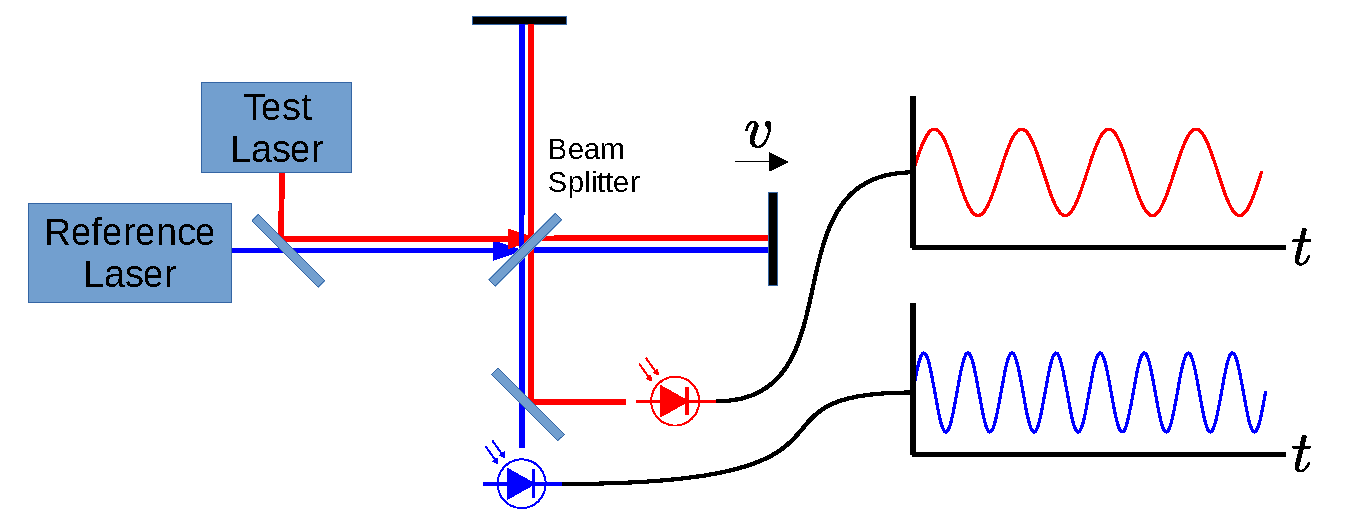
\includegraphics[width=0.9\linewidth]{diagrams/wl_wavemeter}
		\caption{Setup for the simultaneous capture of two interferograms using a Michelson interferometer. The reference laser allows for precise tracking of the translational stage, which can in general have a non-uniform velocity $v(t)$. The recording of these two signals allows for the high-precision measurement of wavelength ratios.}
		\label{fig:wlwavemeter}
	\end{figure}
	
	A simple method to determine the wavelength of the test laser is to count the total number of fringes in each interferogram. This can be accomplished by first shifting the photodetector signal such that the signal no longer has a DC offset and counting the zero crossings. This shifting can be achieved using an analog high-pass filter \cite{Su_analogFilters} immediately after the photodetector. For digitally recorded data, the mean of the data can be subtracted, but improved immunity to laser intensity fluctuations would be given by a digital high pass filter \cite{digital_filter_handbook}, as intensity fluctuations shift the DC offset of the signal in tandem with the amplitude, seen from equation (\ref{wl_sig_monochromatic}). The total number of zero crossings of the two interferograms, $N_\mathrm{Ref}$ and $N_\mathrm{Test}$, give the wavelength of the test laser as
	\begin{equation} \label{wl_wavelength_simple}
		\lambda = \lambda_\mathrm{Ref} \frac{N_\mathrm{Ref}}{N_\mathrm{Test}}
	\end{equation}
	
	Wavelength determination in this manner suffers from counting error \cite{Demtroder2008}. In \ref{sec:wl_wavelength}, we propose a fringe counting method which almost entirely eliminates counting error. While such methods are not new, a fringe counting method tailored for digitally sampled signals and hardware-accelerated computation has not yet been proposed. The method presented in \ref{sec:wl_wavelength} gives both advantages while imposing minimal memory requirements on the acquisition system.
	
	\section{Dynamic Wavelength Reconstruction (DWR)} \label{sec:wl_tracking}
	
	In this section, we introduce a method for Dynamic Wavelength Reconstruction (DWR), which enables the recovery of a time-resolved wavelength $\lambda(t)$ during continuous scans. High-resolution spectroscopic breath characterization requires the acquisition of absorption spectra with high temporal resolution, a requirement that often necessitates the use of rapidly scanning CW lasers. However, the rapid tuning of these lasers introduces a time-dependency in the wavelength $\lambda(t)$, which can complicate the interpretation of the interferogram phase. To address this, we propose the DWR method to extract time-resolved wavelength information from the interferogram signals of a traveling Michelson interferometer. This approach utilizes the phase evolution of a reference interferogram to decouple the effects of optical path delay from wavelength shifts. The following derivation establishes the mathematical framework for this tracking algorithm and demonstrates its asymptotic stability during continuous scans.
	
	The interferogram phase is fundamentally defined by the relationship between the instantaneous wavelength $\lambda(t)$ and the optical path delay $\delta(t)$:
	\begin{equation}
		\phi(t) = \frac{2\pi}{\lambda (t)} \delta(t)
	\end{equation}
	In practice, we observe this phase through the intensity of the bandpass filtered interferogram signal, which can be approximated by a functional form of the type $I(t) \approx A(t) \cos(\phi(t)) $, where $A(t)$ represents a time-dependent amplitude. While $A(t)$ may fluctuate due to experimental instabilities or laser power drift, the zero-crossings of the signal remain robust indicators of the underlying phase evolution, provided that the variations in $A(t)$ are sufficiently slow relative to the oscillation frequency.
	
	The extraction of the instantaneous phase $\phi(t)$ and its derivative $d\phi/dt$ is a well-studied problem in signal processing. While methods such as the Hilbert transform provide a mathematically ideal approach to constructing an analytic signal for frequency estimation, they can be numerically sensitive to sampling jitter and edge effects in high-throughput acquisition, in addition to requiring large computations. Assuming a method of estimating the phase derivative from the sampled signal is available, the time evolution of the phase follows:
	\begin{equation}
		\frac{d\phi}{dt} = \frac{2\pi}{\lambda(t)}\frac{d\delta}{dt} - \frac{2\pi \delta(t)}{\lambda^2(t)}\frac{d\lambda}{dt}
	\end{equation}
	The phase of the reference interferogram is
	\begin{equation}
		\phi_\mathrm{ref}(t) = \frac{2\pi}{\lambda_\mathrm{ref}} \delta(t) + \phi_0
	\end{equation}
	We can solve for the position and velocity from the reference interferogram phase
	\begin{align}
		\delta(t) = \frac{\left(\phi_\mathrm{ref}- \phi_0\right) \lambda_\mathrm{ref}}{2\pi} &&
		\frac{d\delta}{dt} = \frac{\lambda_\mathrm{ref}}{2\pi}\frac{d\phi_\mathrm{ref}}{dt}
	\end{align}
	This gives the derivative of the interferogram phase as
	\begin{equation}
		\frac{d\phi}{dt} = \frac{\lambda_\mathrm{ref}}{\lambda(t)}
		\left[
		\frac{d\phi_\mathrm{ref}}{dt} - \left(\phi_\mathrm{ref} - \phi_0\right) \frac{1}{\lambda(t)}\frac{d\lambda}{dt} 
		\right]
	\end{equation}
	We re-arrange this equation to solve for the derivative of the wavelength
	\begin{equation} \label{wl_tracking_equation}
		\frac{d\lambda}{dt} = \frac{\lambda(t)}{\phi_\mathrm{ref} - \phi_0} \left[
		\frac{d\phi_\mathrm{ref}}{dt} - \frac{\lambda(t)}{\lambda_\mathrm{ref}}\frac{d\phi}{dt}
		\right]
	\end{equation}
	It should be pointed out that the condition for $d\lambda / dt = 0$ is the same as the time derivative of equation (\ref{wl_phase_slope}) for the relation between the phase of the reference and test interferograms of a monochromatic input. However, evaluation of such relations in practice requires a robust method for extracting phase rates from the raw interferometric signal.
	
	\subsection{Phase Extraction From Interferometric Signals}
	The utility of the DWR method relies entirely on the ability to extract the instantaneous phase $\phi(t)$ and its time derivative $d\phi/dt$ from the sampled interferogram. Because the right-hand side of Equation (\ref{wl_tracking_equation}) is driven by the instantaneous rates of change of the reference and test phases, the accuracy of the wavelength reconstruction is fundamentally limited by the precision of these phase estimates.
	
	In our implementation, we treat the zero-crossings of the bandpass-filtered interferogram as noisy, discrete samples of the underlying phase evolution. To transform these stochastic observations into a continuous-time signal suitable for numerical integration, we apply a Savitzky–Golay filter \cite{savitzky_golay_paper} to the sequence of interpolated zero-crossing timestamps. We employ a symmetric polynomial regression approach, performing a smoothing pass on the phase trajectory followed by a differentiation step. This ensures that the estimated $\frac{d\phi}{dt}$ and $\frac{d\phi_\mathrm{ref}}{dt}$ are temporally centered on the true zero-crossing events, providing a sufficiently differentiable signal to satisfy the requirements of the numerical integration used in Equation (\ref{wl_tracking_equation}).
	
	While the process of numerical differentiation typically amplifies high-frequency timing noise, the structure of Equation (\ref{wl_tracking_equation}) provides a natural suppression of these errors through the integration process. This suppression is evident in the error dynamics, where the evolution of the wavelength error $\tilde{\lambda}(t)$ is governed by an exponential decay term: $\tilde{\lambda}(t) = \tilde{\lambda}(0) \exp\left( -\int_{0}^{t} P(t') dt' \right)$. Because the components of $P(t)$ are dominated by the relatively slow-varying phase rates, the integration effectively averages out the stochastic fluctuations in the derivative estimate, preventing them from propagating into the reconstructed wavelength. Consequently, the DWR method produces wavelength tuning curves that remain remarkably smooth despite the underlying stochasticity of the phase derivative estimates.
	
	There remains, however, a fundamental trade-off between the smoothness of the detuning curve and the response time of the recovered wavelength $\lambda(t)$ to fast perturbations. In our implementation, the window size selected for the Savitzky–Golay filtering stage gives an adjustable parameter which can be tuned for different types measurements. For instance; a quick response time might be useful for laser source characterization, and a smooth response is beneficial to serve as a low-noise wavelength axis in spectral measurements. 
	
	\subsection{DWR -- Numerical Solution to the Wavelength Tracking Equation}
	The DWR method is implemented by treating Equation (\ref{wl_tracking_equation}) as a differential equation to be solved numerically. Because the derivative of the wavelength is explicitly defined by the instantaneous phase rates and the current path delay, the reconstruction can be formulated as an initial value problem (IVP). By providing an initial estimate for $\lambda(0)$, the algorithm propagates the wavelength solution forward in time alongside the acquisition of the interferogram.
		
	In practice, this initial wavelength is obtained by pausing the laser scan before tracking begins. Under these conditions, the stationary initial wavelength can be measured using the optimized procedure described in Sec. \ref{sec:wl_ratios}.
	
	Although the initial wavelength is easily determined, the location of the zero delay, expressed as $\phi_0$, remains uncertain. If the laser scan can be halted at the end of the desired spectral region, the final stationary wavelength may also be measured. By treating the unknown $\phi_0$ as a parameter to be determined in a boundary value problem (BVP), we can select the value of $\phi_0$ such that the integrated solution satisfies the terminal boundary condition defined by this measured final wavelength.
	
	We validate the DWR method in Sec. \ref{sec:wl_results_HFS_DWRcomb} by performing a simultaneous three-way comparison within a single experimental scan. During this sweep, we concurrently record the DWR reconstruction, the frequency comb detuning, and the hyperfine spectra. This approach allows for an unambiguous comparison of the reconstructed wavelength against both the established comb-based method (verified in Sec. \ref{sec:wl_results_HFS}) and the physical atomic transitions, all while ensuring that any transient experimental instabilities affect all three measurements identically.
	
%	\subsubsection{Approximate Solution}
%	\begin{align}
%		\frac{d\lambda}{dt} &\approxeq
%		\frac{\tilde{\lambda}}{\phi_\mathrm{ref} - \phi_0}\frac{d\phi_\mathrm{ref}}{dt} - \frac{\tilde{\lambda}}{\phi_\mathrm{ref} - \phi_0}\frac{\lambda(t)}{\lambda_\mathrm{ref}}\frac{d\phi}{dt} \\
%		\frac{d\lambda}{dt} + \lambda(t) g(t) &\approxeq f(t)
%	\end{align}
%	Above we have defined
%	\begin{align}
%		f(t) = \frac{\tilde{\lambda}}{\phi_\mathrm{ref}(t) - \phi_0}\frac{d\phi_\mathrm{ref}}{dt} &&
%		g(t) = \frac{\tilde{\lambda}}{\lambda_\mathrm{ref}\left(\phi_\mathrm{ref}(t) - \phi_0\right)}\frac{d\phi}{dt}
%	\end{align}
%	This can be solved using an integrating factor
%	\begin{equation}
%		\frac{d}{dt}\left[e^{\int g(t') dt'} \lambda(t)\right] = e^{\int g(t') dt'} f(t)
%	\end{equation}
%	This gives the solution
%	\begin{equation}
%		\lambda(t) = e^{-\int_{0}^{t} g(t') dt'} \left[\int_{0}^{t}e^{\int_{0}^{t'} g(t'') dt''} f(t') dt' + \lambda_0\right]
%	\end{equation}
%	The integral in the exponent can be written in the form
%	\begin{align}
%		\int_{0}^{t} g(t') dt' &= \int_{0}^{t} \frac{\tilde{\lambda}/\lambda_\mathrm{ref}}{\phi_\mathrm{ref}(t') - \phi_0} \frac{d\phi}{dt'}dt' \\
%		&= \frac{\bar{\lambda}\phi(t')}{\phi_\mathrm{ref}(t') - \phi_0} \Bigg|_0^t + \int_{0}^{t}\frac{\bar{\lambda}\phi(t')}{\left(\phi_\mathrm{ref}(t') - \phi_0\right)^2}\frac{d\phi_\mathrm{ref}}{dt'}dt' \\
%		\int_{0}^{t} g(t') dt' &= \frac{\bar{\lambda}\phi(t')}{\phi_\mathrm{ref}(t') - \phi_0} \Bigg|_0^t + \frac{1}{\lambda_\mathrm{ref}}\int_{0}^{t}\frac{f(t')\phi(t')}{\phi_\mathrm{ref}(t') - \phi_0}dt'
%	\end{align}
	
	\subsection{Stability Analysis of the Wavelength Tracking Equation}
	To ensure the robustness of the DWR algorithm, we perform a stability analysis on the evolution of (\ref{wl_tracking_equation}) for an imperfect estimate of the initial wavelength. We consider the case where the estimate of the wavelength $\lambda(t)$ deviates the true value $\lambda_0$ by an error term $\tilde{\lambda}(t)$. The evolution of the error term $\tilde{\lambda}(t)$ under the equation (\ref{wl_tracking_equation}) is derived. By showing the conditions under which this error term asymptotically decreases, we find the conditions under which the wavelength tracking method is stable.
	
	Let the instantaneous estimate of wavelength be expressed as
	\begin{equation}
		\lambda(t) = \lambda_0 + \tilde{\lambda}(t)
	\end{equation}
	The true wavelength $\lambda_0$ is the equilibrium solution such that the RHS of \ref{wl_tracking_equation} vanishes, and is the value that gives phase rates which are perfectly matched by the wavelength ratio
	\begin{equation} \label{wl_equilibrium_condition}
		\frac{d\phi_\mathrm{ref}}{dt} = \frac{\lambda_0}{\lambda_\mathrm{ref}}\frac{d\phi}{dt}
	\end{equation}
	Substituting $\lambda(t) = \lambda_0 +  \tilde{\lambda}(t)$ into the governing equation (\ref{wl_tracking_equation}), we obtain:
	\begin{equation}
		\frac{d(\lambda_0 + \tilde{\lambda})}{dt} = \frac{\lambda_0 + \tilde{\lambda}}{\phi_\mathrm{ref} - \phi_0} \left[ \frac{d\phi_\mathrm{ref}}{dt} - \frac{\lambda_0 + \tilde{\lambda}}{\lambda_\mathrm{ref}}\frac{d\phi}{dt} \right]
	\end{equation}
	Since $\lambda_0$ is constant, $\frac{d(\lambda_0 + \tilde{\lambda})}{dt} = \frac{d\tilde{\lambda}}{dt}$. Expanding the terms and applying the equilibrium condition from Eq. (\ref{wl_equilibrium_condition}), we can neglect higher-order terms of $\delta$ (i.e., $\delta^2 \approx 0$) to linearize the dynamics.
%	The equation simplifies to
%	\begin{equation}
%		\frac{d\delta}{dt} \approx \frac{\lambda_0}{\phi_\mathrm{ref} - \phi_0} \left[ \underbrace{\frac{d\phi_\text{ref}}{dt} - \frac{\lambda_0}{\lambda_\text{ref}}\frac{d\phi}{dt}}_{= 0} - \frac{\delta}{\lambda_\text{ref}}\frac{d\phi}{dt} \right]
%	\end{equation}
	Using (\ref{wl_equilibrium_condition}) yields a linear homogeneous differential equation for the time-dependent error $ \tilde{\lambda}(t)$
	\begin{equation}
		\frac{d\tilde{\lambda}}{dt} + \underbrace{\left[ \frac{\lambda_0}{\lambda_\mathrm{ref}(\phi_\mathrm{ref} - \phi_0)} \frac{d\phi}{dt} \right]}_{\begin{matrix}P(t)\end{matrix}} \tilde{\lambda} = 0
	\end{equation}
	This is in the form of a first-order decay equation $\frac{d\tilde{\lambda}}{dt} + P(t)\tilde{\lambda} = 0$. The stability of the system depends on the sign of the coefficient $P(t)$. A stable evolution then requires that $\frac{d\phi}{dt}$ has the same sign as $(\phi_\mathrm{ref} - \phi_0)$, indicating that we must always scan away from the point of zero optical phase delay. Under this assumption, it follows that $P(t) > 0$ for all $t > 0$. Consequently, the solution for the error is
	\begin{equation}
		\tilde{\lambda}(t) = \tilde{\lambda}(0) \exp\left( -\int_{0}^{t} P(t') dt' \right)
	\end{equation}
	As $t$ increases, $ \tilde{\lambda}(t) \to 0$, implying that the tracking algorithm is \textit{asymptotically stable} for scans of increasing optical path delay magnitude. Any perturbation in the wavelength estimate, due to electronic noise or mechanical jitter, will exponentially decay, allowing the system to converge back to the true wavelength.
	
	The stability analysis assumes a well-defined coefficient $P(t)$. However, the term $(\phi_\mathrm{ref}(t) - \phi_0)$ appears in the denominator of the error dynamics. The singularity $\phi_\mathrm{ref} = \phi_0$ occurs for zero optical path delay $\delta =0$. In practice, this simply means that scans across the point where the lengths of the two interferometer arms are equal should be avoided.
	
	\subsubsection{Sensitivity to the Zero-Delay Offset $\phi_0$}
	While the algorithm is robust against errors in the initial wavelength estimate $\lambda(0)$ when scanning away from the zero delay point $\delta = 0$, the accuracy of the reconstruction is highly sensitive to the location of this point through the reference phase offset, $\phi_0$. In our BVP approach, we treat $\phi_0$ as a parameter to be determined such that the integrated solution satisfies a known terminal boundary condition. 
	
	%To quantify the sensitivity, consider a case where the wavelength varies linearly, $\lambda(t) = \beta t + \lambda_i$, and the true zero-delay phase is $\phi_0$. If we introduce an error $\phi_e$ into our estimate of the offset, such that $\hat{\phi}_0 = \phi_0 + \phi_e$, this error propagates through the integration of Equation (\ref{wl_tracking_equation}). Because $\phi_0$ appears in the denominator of the $P(t)$ term within the error dynamics, a mismatch in $\phi_0$ prevents the true equilibrium condition from being met. This results in a systematic divergence between the reconstructed $\hat{\lambda}(t)$ and the true $\lambda(t)$ as the optical path delay increases. 
	
	%While the sensitivity of the reconstruction to $\phi_e$ necessitates a robust estimation strategy, it is important to note that $\phi_0$ can, in principle, be determined via independent physical references, such as an absolute position encoder or a frequency comb input. Such external measurements provide a direct way to anchor the phase evolution to a known coordinate. However, for extended scans, the reliance on these external sensors introduces secondary error sources, such as encoder resolution limits or cumulative mechanical drift. 
	
	%Crucially, the BVP approach remains highly effective even in the presence of such external references because the impact of an initial $\phi_0$ mismatch diminishes as the scan progresses. As the optical path delay $\delta(t)$ increases, the relative influence of the offset error on the instantaneous phase rate $\frac{d\phi}{dt}$ decreases, causing the discrepancy in the reconstructed $\frac{d\lambda}{dt}$ to asymptotically vanish. Thus, the BVP method provides a self-consistent way to utilize terminal wavelength measurements to correct for any residual uncertainty in the zero-delay point, ensuring high-fidelity reconstruction across the entire scanned range.
	
	\section{Fourier Transform Spectroscopy (FTS)} \label{sec:wl_FTIR}

	We discuss how the Michelson interferometer can be interchangeably used as a broadband spectrum analyzer, or wavemeter. This type of interferogram analysis will be used for two purposes: calibration of reference laser wavelength, and motivating another analysis technique that will be later presented in Ch. \ref{chap:comb_ceas}.
	
	The interferogram recorded by the photodetector for a monochromatic source was described in Eq. (\ref{wl_sig_monochromatic}). This result can be generalized to a broadband light source by treating the input field as a continuous superposition of monochromatic components. Neglecting phase-coherent beating between these components (see Sec. \ref{sec:beat_notes}), the total interferogram intensity $I(t)$ is obtained by integrating the individual spectral contributions over the frequency spectrum:
	\begin{align} \label{wl_interferogram_incoherent}
		I(t) &= \int_{0}^{\infty} |\mathcal{A}(\omega)|^2 \left[ 1 + \cos\big(k(\omega)\delta(t) + \phi_0(\omega)\big) \right] d\omega \nonumber \\
		&= I_0 + \int_{0}^{\infty} |\mathcal{A}(\omega)|^2 \cos\left(\frac{2\omega vt}{c} + \phi_0(\omega)\right) d\omega
	\end{align}
	where we have assumed the dispersionless relation $k = \omega/c$ and a constant scanning velocity $v$. Here, $I_0$ represents the time-averaged power of the input light, while $\mathcal{A}(\omega)$ denotes the complex spectral amplitude of the input field $E_\mathrm{in}(t) = \mathcal{A}(\omega) e^{-i\omega t}$.
	
	The phase function $\phi_0(\omega)$ accounts for frequency-dependent phase delays introduced by optical elements, such as the beam splitter and mirrors. In FTS, the Michelson interferometer should be configured symmetrically to ensure that both arms impart identical phase delays, thereby minimizing any non-linear frequency dependence in $\phi_0(\omega)$. It is important to note that a linear term in $\phi_0(\omega)$ is physically equivalent to an additional optical path delay. Consequently, we proceed under the assumption that the interferometer is designed such that $\phi_0(\omega)$ is effectively constant, denoted as $\phi_0$.
	
	The quantity $|\mathcal{A}(\omega)|^2$ represents the optical power spectrum. If this spectrum can be resolved, the interferometer functions as a traditional spectrometer by decomposing the input light into its constituent frequency (or wavelength) components. Assuming the interferometer arm scans at a constant velocity $x(t) = vt$, each spectral component $\omega$ is mapped onto an interferogram oscillation with a frequency $\omega_\mathrm{int} = 2\omega v/c$. This frequency arises from the interference between the stationary component of the light and the Doppler-shifted component reflected from the moving mirror. Consequently, the optical power spectrum $|\mathcal{A}(\omega)|^2$ can be recovered by performing a Fourier transform on the modulated part of the interferogram
	\begin{equation}
		\left|\mathcal{A}(\omega)\right|^2 = \mathcal{F}_t\left[I(t) - I_0\right](\omega)
	\end{equation}
	
	\subsection{Processing of Interferograms Into Optical Spectra}
	
	In practice, the translation stage does not maintain a perfectly constant velocity, leading to a time-dependent scanning rate $v(t)$. Such fluctuations introduce non-linear phase modulation in the interferogram, which manifests as spectral broadening and artifacts in the recovered power spectrum if a standard Fourier transform is applied. To address this, we decouple the measurement of the stage position from the signal processing of the intensity. We utilize the high-resolution interferogram of the reference laser to track the instantaneous optical path delay $\delta(t)$ with high precision. This provides a continuous, non-uniform temporal map of the physical displacement.
	
	The recovery of the power spectrum can be approached through two distinct numerical strategies, each offering different advantages. One may employ a Type-1 Non-Uniform Fourier Transform (NUFFT) to directly extract spectral content from the irregularly sampled time-series. Alternatively, one can perform a numerical re-sampling step to linearize the signal sampling. By using cubic spline interpolation to map the intensity onto a strictly uniform grid in the optical path delay domain, $\delta$, the signal becomes compatible with standard Fast Fourier Transform (FFT) algorithms. In this work, we utilize the latter approach. By leveraging the high-resolution position information provided by the reference laser interferogram, we interpolate the test-laser signal onto a uniform $\delta$-grid, thereby ensuring spectral integrity despite any mechanical non-uniformities in the translation stage velocity. This method is computationally efficient, and gives results which are mostly indistinguishable from those obtained by the NUFFT when the signal is sampled in a manner that allows for effective interpolation.
	
	\subsection{Assumption of Incoherence and Frequency Comb Inputs}
	
	For general input sources that exhibit coherence between different spectral components—such as a frequency comb—the detected intensity can be expressed as a time-averaged autocorrelation. Let $T = \delta/c$ represent the additional time delay introduced by the scanning interferometer arm. The detector intensity is then given by:
	\begin{equation}
		I(t, T) = \underbrace{2\Bigl<  \left|E(t)\right|^2 \Bigr>}_{I_0} + \underbrace{2 \mathrm{Re}\,\Bigl< E(t) E^*(t-T) \Bigr>}_{\Gamma(T)}
	\end{equation}
	where $I_0$ is the time-averaged power and $\Gamma(T)$ is the complex field autocorrelation function. The derivation of Eq. (\ref{wl_interferogram_incoherent}) assumes that the measurement window is sufficiently long to treat the field as wide-sense stationary (WSS); this ensures that the statistical properties of the source are invariant over the scan, such that the autocorrelation $\Gamma$ depends only on the relative delay $T$. Under this assumption, the interferogram output corresponds to the real part of the field autocorrelation function. Consequently, the optical power spectrum can be recovered from the Fourier transform of the mean-subtracted signal via the Wiener–Khinchin theorem \cite{book_born_and_wolf_princpOptics}.
	
	In practical applications involving frequency combs, the requirement for wide-sense stationarity is satisfied when the measurement duration significantly exceeds both the period of the comb's repetition rate ($1/f_{\text{rep}}$) and the characteristic timescale of any source instabilities. While a frequency comb consists of discrete, phase-coherent modes, the detector's finite bandwidth $B$ typically acts as a low-pass filter such that $B \ll f_{\text{rep}}$. This prevents the photodetector from resolving the rapid intensity fluctuations (the "beats") occurring at the repetition frequency \cite{dual_comb_review}, effectively performing an integration over the individual comb lines. Consequently, the detector perceives a continuous spectral envelope rather than a series of discrete pulses. As long as the mechanical scan is sufficiently slow to average over these high-frequency components, the detected signal remains a stable representation of the time-averaged autocorrelation, allowing for the robust extraction of broadband absorption features through the Fourier transform of the interferogram.
	
	\begin{figure}[H]
		\centering
		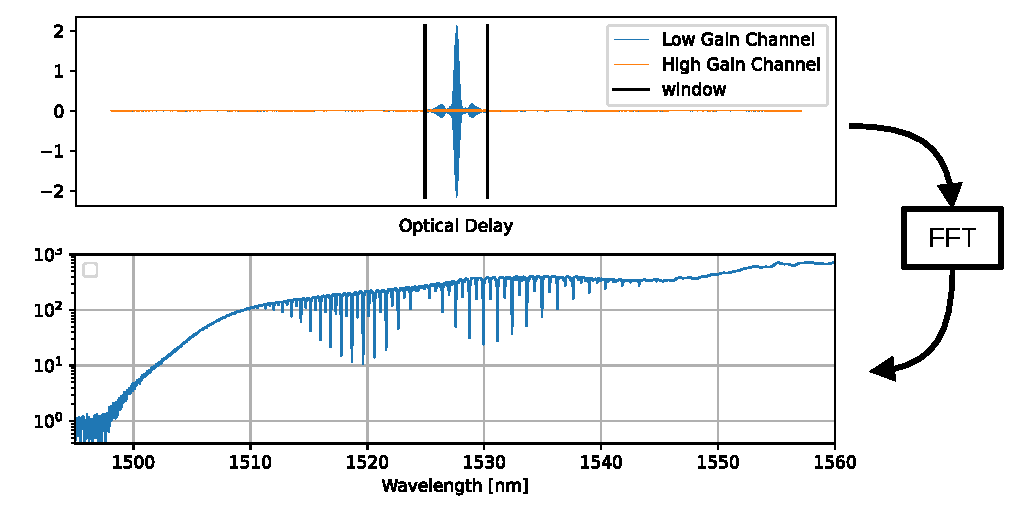
\includegraphics[width=1.0\linewidth]{diagrams/wl_FTIR_acetylene}
		\caption{The transformation of an interferogram into an optical spectrum. Shown is a measurement of the absorption spectrum of acetylene using the interferometer shown in Fig. \ref{fig:wlwavemetersetup} with an absorption cell in the path of the input laser. The upper plot shows a zoomed region of the time-domain interferograms captured by the Michelson interferometer, and the lower pane is the resulting spectrum showing the clear absorption features of acetylene. The Fourier transform relates the interferogram to the optical spectrum. Not shown is the process of converting the reference laser interferogram into the optical delay, a prerequisite for using the FFT algorithm shown here. The absorption lines can clearly be resolved as the sharp dips in the optical intensity. For a species having well-cataloged absorptions, the locations of these absorption lines serve as well-defined wavelength markers.}
		\label{fig:wl_ftir_acetylene}
	\end{figure}
	
	
%	\subsection{Summary of Measurement Regimes}
%	The distinction between the two measurement modes is summarized in Table \ref{tab:measurement_modes}. While the hardware configuration remains identical, the analytical objective shifts from a scalar estimation of a ratio (Wavemeter) to a functional reconstruction of a distribution (FTIR).
%	
%	\begin{table}[H]
%		\centering
%		\caption{Comparison of Wavemeter and FTIR measurement regimes.}
%		\label{tab:measurement_modes}
%		\begin{tabular}{lll}
%			\hline
%			\textbf{Feature} & \textbf{Wavemeter} & \textbf{FTIR Spectrometer} \\ \hline
%			Input Spectrum & Monochromatic ($\delta$-function) & Broadband (Continuous) \\
%			Signal Type & Sinusoid & Complex Interferogram \\
%			Analytical Goal & Ratio estimation ($\lambda/\lambda_{\text{ref}}$) & Spectral reconstruction $\mathcal{A}^2(\omega)$ \\
%			Mathematical Tool & Slope determination/Zero-crossing & Fourier Transform \\
%			Primary Constraint & Phase stability and $v$ precision & Total scan range (OPD) \\ \hline
%		\end{tabular}
%	\end{table}
	
	\section{Experimental Apparatus for Interferometric Wavelength Measurement}
	Most of the wavelength measurements conducted in this work were performed using a Michelson interferometer. The basic configuration was described in Sec. \ref{sec:wl_wavelength}, and here we elaborate on the specific optical layout.
	
	\begin{figure}[H]
		\centering
		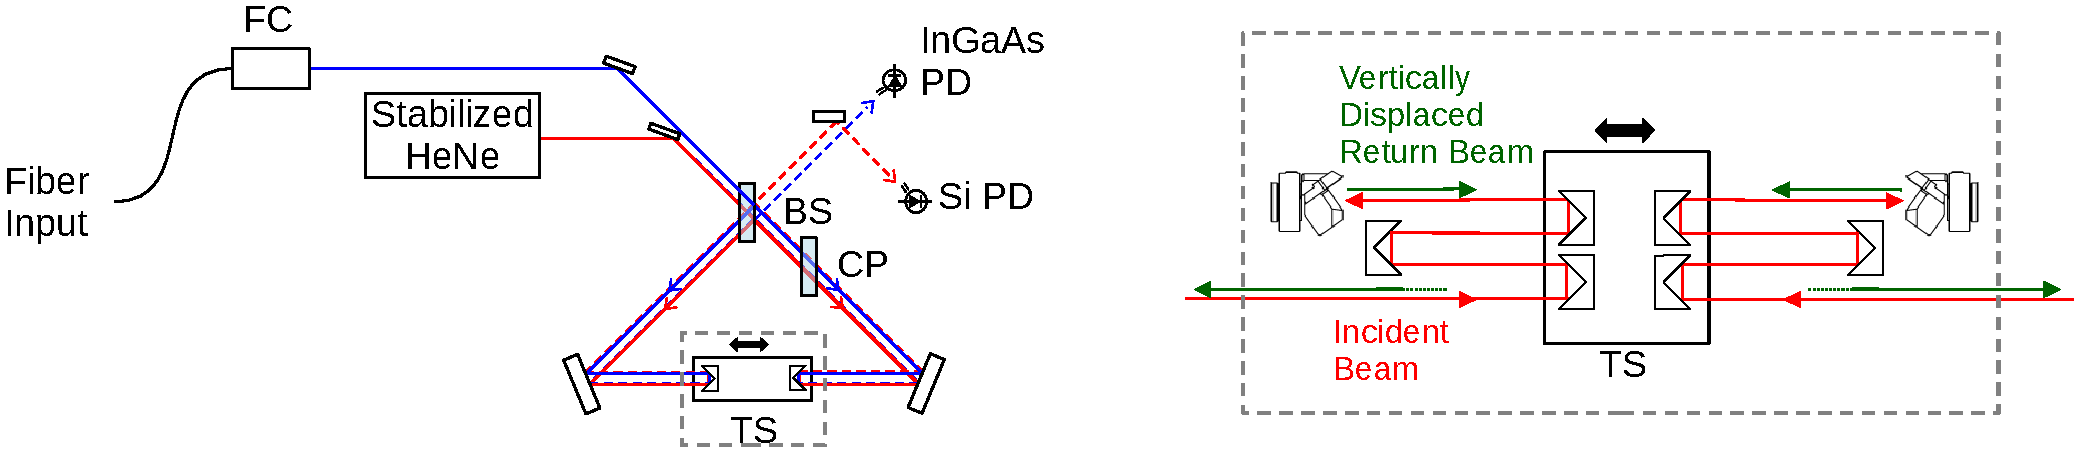
\includegraphics[width=1.0\linewidth]{diagrams/wl_wavemeter_setup}
		\caption{Layout of a symmetrical Michelson interferometer optimized to for the minimization of the relative phase shift between the two arms. The folding geometry enables long delay scans to be captured, enabling high resolution measurements within a compact apparatus. Another configuration used in this work is shown in Fig. \ref{fig:hfs_setup}, where an asymmetrical configuration is used. The central beam-splitter (BS) and compensation plate (CP) form two arms of variable distance which is scanned by a translation stage (TS). The retro-reflector configuration is such that the return beam from each arm is anti-parallel and displaced. Two spatially separated reference beams are obtained at BS; one is directed to a Si photodiode (PD), the other is counter-propagating to the IR beam (shown in blue) input. The two-fold IR output of BS are directed to an InGaAs balance detector (BD) with the assistance of a dichroic mirror (DM).}
		\label{fig:wlwavemetersetup}
	\end{figure}
	
	\subsection{Calibration of Reference Laser Wavelength} \label{sec:wl_ref_calibration}
	This section describes two procedures for calibrating the reference laser wavelength within the apparatus shown in Fig. \ref{fig:wlwavemetersetup}. Both methods involve measuring a known absorption peak simultaneously with the wavelength and applying a correction factor to ensure that the observed peak position aligns precisely with the recorded wavelength.
	
	Wavelength determination via Eq. (\ref{wl_wavelength_slope}) provides an estimate of the CW wavelength as
	\begin{equation}
		\lambda = \lambda_\mathrm{ref} \frac{d\phi_\mathrm{ref} / dt}{d\phi / dt}
	\end{equation}
	We define a multiplicative wavelength correction factor such that
	\begin{equation} \label{wl_correction_factor}
		\lambda_\mathrm{actual} = \beta \lambda_\mathrm{meas}
	\end{equation}
	The factor $\beta$ can then absorb uncertainty in the reference laser wavelength, refractive index mismatches between the sampling region and wavelength measurement region, as well as dispersion in the air between the reference and infrared laser wavelengths.
	
	Using a CW laser capable of wavelength scanning, this calibration can be performed by conducting a scan across a well-documented molecular absorption line. Provided the laser maintains sufficient interaction length with the sample, the procedure involves recording the transmitted light intensity as a function of the apparatus's measured wavelength. Since the objective is solely to identify the center of the absorption feature, it is not necessary to calibrate the absorption magnitude derived from Eq. (\ref{beer_absorp}).
	
	Wavelength calibration can also be achieved using a broadband source, provided that molecular absorption features are imprinted onto the spectrometer's input light, similar to the measurement shown in Fig. \ref{fig:wl_ftir_acetylene}. Performing a Fourier transform spectroscopy (FTS) analysis on the resulting interferograms (Sec. \ref{sec:wl_FTIR}) of both the reference laser and the input light yields a spectrum with a wavelength scale dependent on $\lambda_\mathrm{ref}$. Correction of the retrieved wavelength scale to match known absorption features then yields a value of the correction factor $\beta$.
	
	Shown in Fig. \ref{fig:wl_referencelaser_calib} is a configuration to allow calibration of a wavemeter which is capable of performing FTIR scans. This is done by using a single mode fiber to ensure that the input light does not suffer from pointing error between input source changes. By performing the FTS measurement of a known spectrum, we yield a correction factor $\beta$ of the reference laser wavelength which can then be used to measure the CW laser wavelength.
	
	\begin{figure}[H]
		\centering
		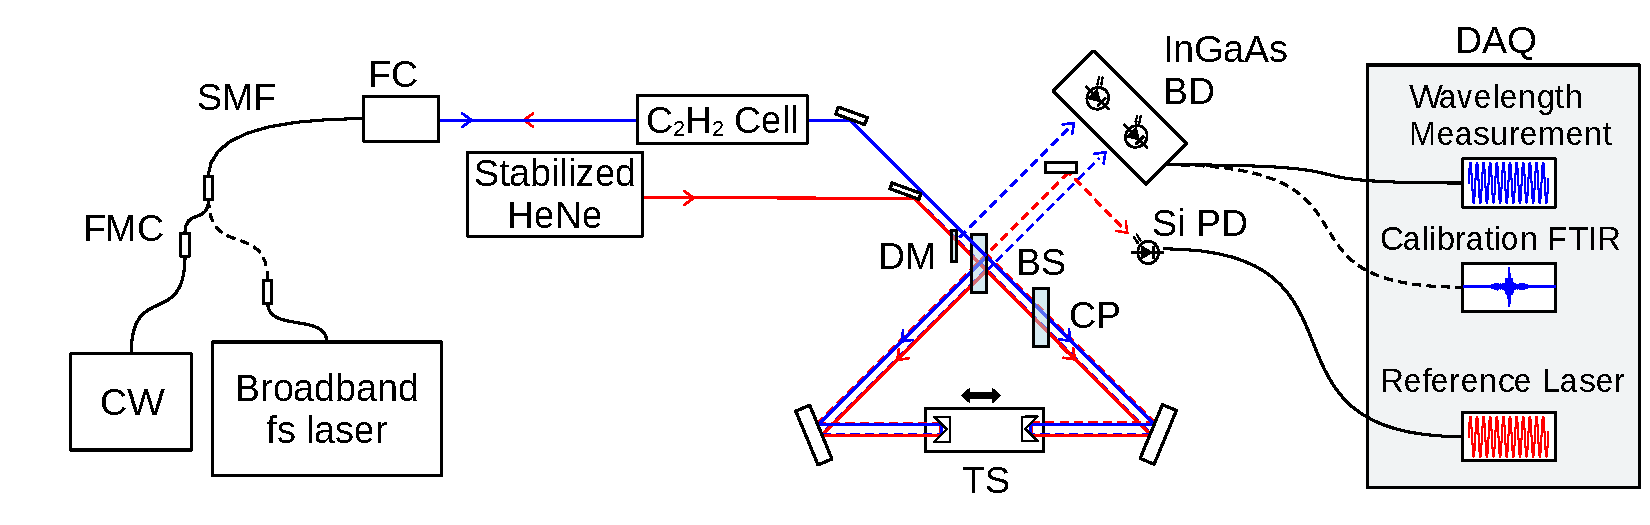
\includegraphics[width=1.0\linewidth]{diagrams/wl_referenceLaser_calib}
		\caption{Calibration of the reference laser wavelength by performing FTS on the broadband input light provided by a fs laser. The IR input of the instrument is connected via a single mode fiber (SMF) to ensure consistent beam profile and pointing direction between laser source changes, which are accomplished by mannually changing a fiber mating connector (FMC). The IR beam is propagated through an acetylene filled cell in a manner anti-parallel to the visible reference laser.}
		\label{fig:wl_referencelaser_calib}
	\end{figure}
	
	\section{Direct Optical Frequency Measurement}
	In this section, the frequency comb is described as a tool for the direct measurement of optical frequencies, as opposed to the measurement of wavelength. This is achieved by forming a beat-note (see \ref{sec:beat_notes}) between a target CW laser and a stabilized frequency comb.
	
	\subsection{The Frequency Comb as a Metrological Benchmark} \label{sec:wl_combs}
	In this chapter, the frequency comb is utilized as a high-precision metrological reference to validate the accuracy of the numerical calibration methods presented in the preceding sections. While the generation of the comb itself is not the focus of this research, its role as an electronic frequency ruler allows for the rigorous assessment of systematic uncertainties in our wavelength reconstruction algorithms.
	
	A frequency comb provides a coherent bridge between the optical and radio-frequency (RF) domains through a series of precisely spaced spectral lines defined by
	\begin{equation} \label{wl_comb_modes}
		f_m = f_\mathrm{ceo} + m f_\mathrm{rep},
	\end{equation}
	where $m$ is an integer. In our experimental configuration, the repetition rate $f_\mathrm{rep}$ is stabilized to a commercial Rubidium (Rb) frequency standard via a feedback loop to a piezoelectric actuator on the laser cavity. This stabilization ensures that the mode spacing remains fixed relative to a highly stable RF reference, providing a stationary spectral grid against which the accuracy of our tracking algorithms can be tested.
	
	The relationship between the time-domain pulse train and its frequency-domain representation is illustrated in Figure \ref{fig:wl_combdiagram}. In the upper pane, the rapid electric field oscillations are shown underneath a black envelope, where the time between pulses $T$ and the phase slippage $\Delta \phi$ between the carrier and the envelope directly dictate the structure of the comb. As shown in the bottom pane, these temporal parameters define the spacing and offset of the spectral lines.
	
	It should be noted that because the carrier-envelope offset frequency, $f_\mathrm{ceo}$, is not actively stabilized, we do not perform absolute optical frequency measurements. Instead, we utilize the comb to measure the relative detuning of the laser frequency from the comb modes. To ensure the integrity of these measurements, an $f\text{-}2f$ interferometer is employed to monitor the $f_\mathrm{ceo}$ drift. By doubling the frequency of a low-frequency comb mode and beating it against a higher-frequency mode, the $f_\mathrm{ceo}$ can be extracted and bounded, allowing any residual offset shifts to be accounted for during post-processing.
	
	The utility of the comb in this chapter relies on its ability to generate precise frequency markers during a continuous laser scan. When the comb beam is overlapped with a CW laser beam, the resulting beat note contains multiple RF peaks corresponding to the differences between the CW laser frequency and adjacent comb modes. To determine the frequency of the laser relative to the nearest comb mode, it is necessary to identify the mode number $\mathrm{int}(m)$. If $f_\mathrm{rep}$ is stabilized sufficiently well, a small intentional scan of the repetition rate, $\Delta f_\mathrm{rep}$, will produce a measurable frequency shift of $m\Delta f_\mathrm{rep}$. This frequency multiplication allows for the unambiguous determination of $m$, and consequently, the frequency detuning relative to the comb structure. A similar approach was demonstrated in \cite{ours_single_mg_comb_line}, where the absolute frequency of a single $^{25}\mathrm{Mg}^+$ ion transition was measured with record precision using a single comb line.
	
	However, this determination is limited by the stability of the carrier-envelope offset; if $f_\mathrm{ceo}$ is not stabilized to single-Hz levels, the repetition rate change $\Delta f_\mathrm{rep}$ must be kept on that same order to avoid ambiguity from the repeating modes. To avoid the additional complexity introduced by $f_\mathrm{ceo}$ stabilization, we present the method in Section \ref{sec:wl_optical_detuning}, which allows for the determination of relative optical detuning without the requirement for tight stabilization of the offset frequency.
	
	\begin{figure}[H]
		\centering
		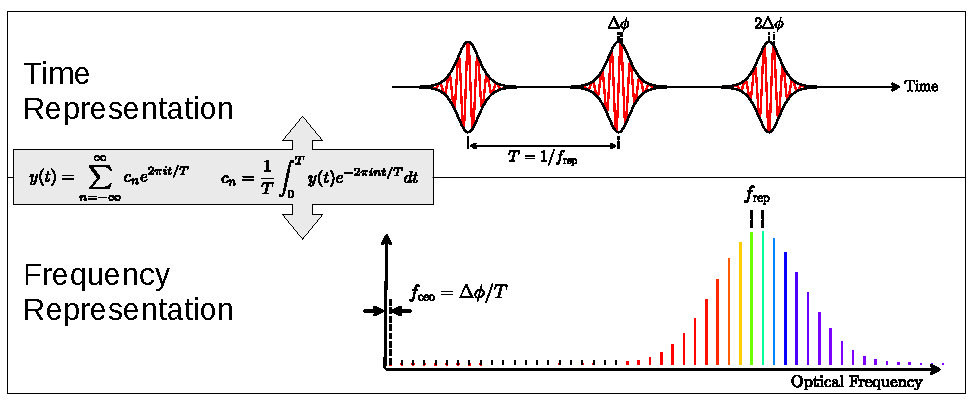
\includegraphics[width=0.9\linewidth]{diagrams/wl_comb_diagram}
		\caption{The complementary time-domain (upper) and frequency-domain (lower) representations of a stabilized laser pulse train are shown connected by the Fourier series. In the upper pane, the rapid electric field oscillations are shown in red underneath a black envelope. The time between these pulses $T$ and the phase slippage $\Delta \phi$ between the red carrier and the black envelope are directly related to the comb structure shown in the bottom pane. By stabilizing the frequency-domain comb parameters $f_\mathrm{CEO}$ and $f_\mathrm{rep}$, easily measured and counted by standard laboratory equipment, the rapid electric field oscillations in the time domain are also stabilized and become countable.}
		\label{fig:wl_combdiagram}
	\end{figure}
	
	\section{Relative Optical Detuning for a Scanning Laser} \label{sec:wl_optical_detuning}	
	We propose a method that can directly recover the relative detuning of a laser in units of optical frequency while imposing only relaxed requirements on the carrier-envelope offset of the comb. We assume that the comb is repetition-rate stabilized, such that all comb modes drift in unison with the carrier-envelope offset frequency. If a CW laser is scanned across these comb modes, the interference between the two beams would produce a repeating pattern of bursts on a low-bandwidth detector; each burst would indicate when the CW laser frequency crosses a comb mode, effectively creating a frequency ruler with spacing $f_\mathrm{rep}$. However, this direct detection scheme suffers from the inherent difficulties of near-DC measurements. In this regime, electronic noise is at its peak, and the signal integrity is highly susceptible to laser intensity fluctuations.
	
	We improve upon this by shifting the detection into a narrow band centered around $f_\mathrm{rep}/4$. As illustrated in the upper portion of Figure \ref{fig:wl_comb_detuning}, this is achieved using a combination of a mixer, a frequency generator, and a low-pass filter (LPF) to form a narrow band-pass filter. This circuit acts on the output of a photodetector, which must possess sufficient bandwidth to capture the interference between the CW and comb beams. The resulting output provides markers in the form of a chirp signal with a sharply peaked envelope that occurs every time the CW laser frequency is at a distance of $f_\mathrm{rep}/4$ from the nearest comb line. 
	
	The marker locations in the optical frequency domain are illustrated in the lower portion of Figure \ref{fig:wl_comb_detuning} by the blue marker lines. In this scheme, the scanning laser produces markers that appear with an even spacing of $f_\mathrm{rep}/2$. This approach provides higher resolution than DC detection and offers the significant advantage of being essentially immune to low-frequency laser intensity fluctuations. The red trace in the top-right inset of Figure \ref{fig:wl_comb_detuning} shows a recorded oscilloscope trace from our experimental setup, demonstrating a clean and well-resolved ruler signal.
	
	The efficacy of this method was demonstrated through measurements of atomic hyperfine structure (HFS), where it provided reliable estimates of optical detuning even while the carrier-envelope offset of the comb remained free-running. Using an $f\text{-}2f$ interferometer, we determined that during our scans, the carrier-envelope offset changed by an amount less than $f_\mathrm{rep}/8$. This drift caused only minor disruptions to the even spacing of the frequency ruler and was found to average out effectively across multiple scans. The following sections provide an extensive validation of this measurement technique through the characterization of xenon and rubidium spectra.
	
	\begin{figure}[H]
		\centering
		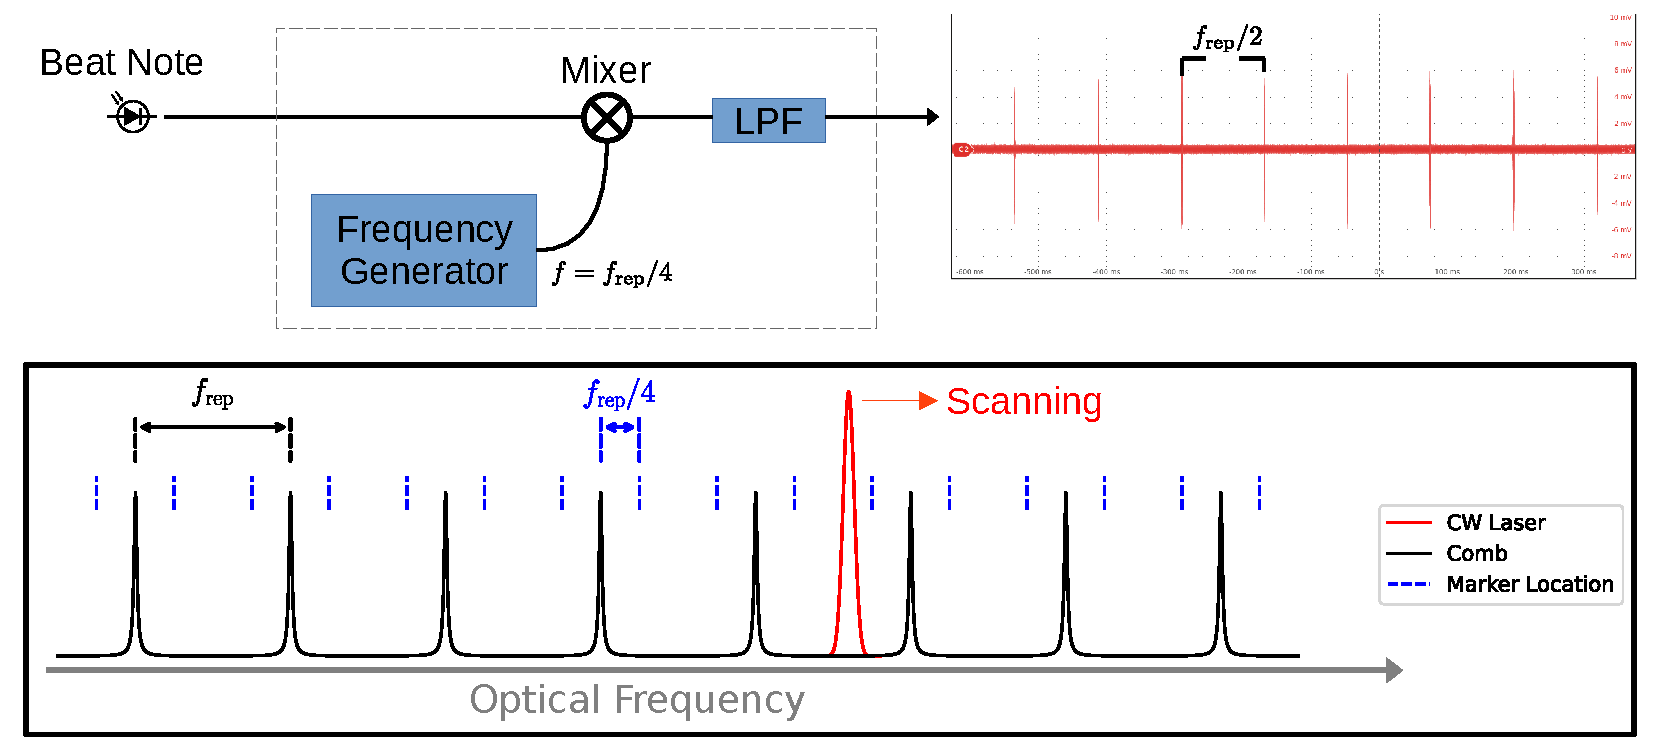
\includegraphics[width=1.0\linewidth]{diagrams/wl_comb_detuning}
		\caption{Shown is a scheme for generating electronic markers which indicate the relative detuning of a scanning CW laser in increments of one-half the repetition rate of a frequency comb. The upper right inset features an experimentally recorded electronic marker signal, showing clearly resolved marker locations and small noise.}
		\label{fig:wl_comb_detuning}
	\end{figure}
	
	\section{Validation of Novel Methods With Hyperfine Structure Measurements}\label{sec:wl_results_HFS}
	While the primary objective of this work is to develop technologies for breath analysis, the precision requirements of molecular spectroscopy are often much lower than those of atomic physics; therefore, we utilize the Doppler-free hyperfine structure (HFS) measurements presented in this section as a far more rigorous testing ground for our wavelength and optical frequency calibration.
	
	The experimental procedure for obtaining Doppler-free HFS using saturated absorption spectroscopy follows the methodology established in \cite{ours_xe_paper}; consequently, the specific details regarding laser preparation and saturated absorption spectroscopy are omitted here to focus on the calibration-specific results. The primary distinction between the measurements presented of Xenon presented in this chapter and those reported in \cite{ours_xe_paper} lies in the calibration of the wavelength (or frequency) axis. While the previous work relied on an etalon with a known free spectral range (FSR) for wavelength referencing, the current approach utilizes the heterodyne marker generation technique described in Section \ref{sec:wl_optical_detuning} and the DWR procedure presented in Sec. \ref{sec:wl_tracking}. Both the comb-based method and DWR provide a more direct and streamlined calibration process, reducing the systematic uncertainties associated with the mechanical stability and interpolation of etalon-based references.
	
	\subsection{Experimental Setup}
	
	The CW laser used in this experiment is the same used in \cite{ours_xe_paper}, and is a Coherent CR899 configured as a Ti:Sapphire solid state CW laser. This laser is capable of mode-hop free tuning over a range of 20GHz. The output beam of this laser is sent to two calibration sources: a Michelson interferometer which performs dynamic wavelength reconstruction of the scanning laser wavelength, and a beat-note with a frequency comb which enables direct optical detuning measurements. The remaining beam is sent to a saturated absorption spectroscopy experiment in which the hyperfine structure of Rb is measured.
	
	The frequency comb consists of an 80 MHz Ti:Sapphire oscillator with built-in f-2f interferometer. This oscillator was modified to enable repetition rate stabilization by cavity length control using a piezoelectric actuator. The repetition rate was locked to Rb-stabilized oscillator, and the carrier envelope offset was left free-running.
	
	%In order to accurately measure the hyperfine structure of Xe, thermal motions of Xe atoms in the measurement cell must be overcome, as this Doppler broadening obscures closely spaced transition frequencies under normal conditions. This goal was accomplished via the method of Lamb-dip saturation spectroscopy \cite{saturated_absorption_spec_Hansch}. The experiment is carried out in the configuration with counter-propagating pump and probe beams (Fig.2), where atoms having velocity vectors perpendicular to both beams preferentially contribute to the signal, thus cancelling out first-order Doppler shifts of transition frequencies.
	
	\begin{figure}[H]
		\centering
		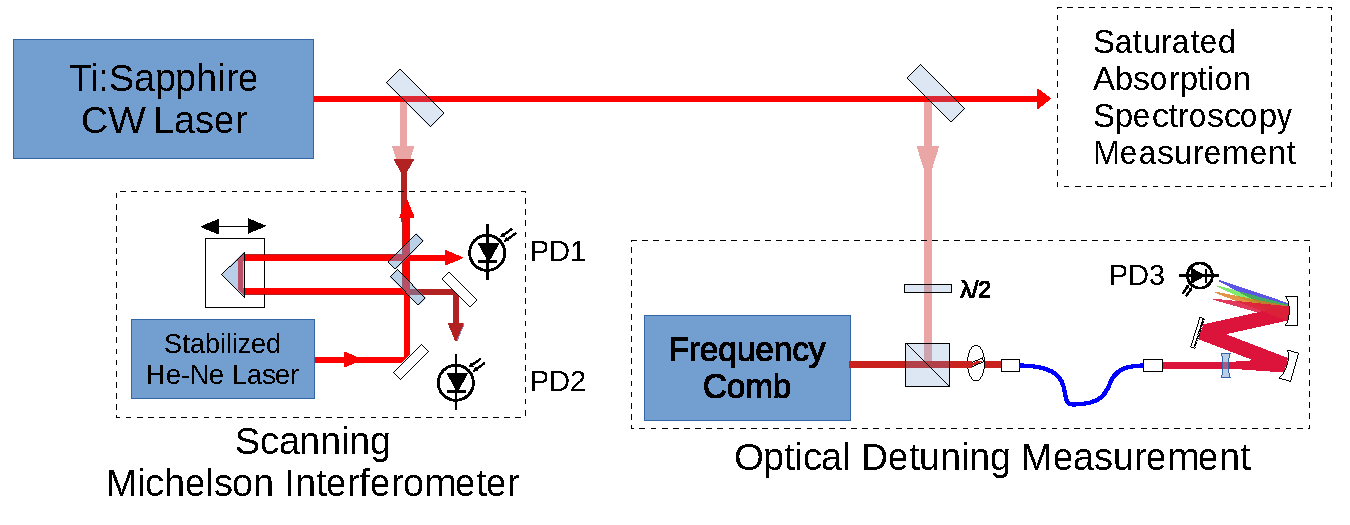
\includegraphics[width=0.9\linewidth]{diagrams/hfs_setup_simp}
		\caption{Experimental apparatus for the simultaneous calibration of a scanning CW laser using the two proposed methods. By calibrating the scans of xenon and rubidium hyperfine spectra, the two methods are validated. The CW laser source is a Coherent CR-899 configured to operate with a solid state gain medium. In the left block a Michelson interferometer configuration, typically used for wavelength measurement, is shown measuring a sampled portion of the same laser light used to perform the comb calibration and saturated absorption spectroscopy. In the right block, the optical beat note between the laser and a repetition-rate stabilized frequency comb is detected, allowing for the direct measurement of the optical detuning.}
		\label{fig:hfs_setup}
	\end{figure}
	
	\subsection{Validation of Comb Detuning Method}
	
	The accuracy of the frequency-comb-based detuning method was validated through the extraction of hyperfine constants ($A$ and $B$) and isotope shifts for several transitions in rubidium and xenon. The experimental procedure follows the methodology established in \cite{ours_xe_paper}; therefore, the specific details regarding laser preparation and saturated absorption spectroscopy are omitted here to focus on the calibration-specific results. 
	
	The primary distinction between the measurements presented in this chapter and those reported in \cite{ours_xe_paper} lies in the calibration of the frequency axis. While the previous work relied on an etalon with a known free spectral range (FSR) for wavelength referencing, the current approach utilizes the heterodyne marker generation technique described in Section \ref{sec:wl_optical_detuning}. This comb-based method provides a more direct and streamlined calibration process, reducing the systematic uncertainties associated with the mechanical stability and interpolation of etalon-based references.
	
	The experimental workflow involved fitting the measured saturated absorption profiles to extract peak positions, which were then compared to the theoretical model used in \cite{ours_xe_paper}. The results for the isotope shifts of six xenon isotopes, along with two independent measurements of the lower-state hyperfine constants, are presented in Figure \ref{fig:hfs_xelitmargs}. These results demonstrate excellent agreement with previously published literature. 
	
	Notably, the values obtained here are consistent with those reported in \cite{ours_xe_paper}. Results for the isotope shift of six xenon isotopes, as well as two independent measurements of the lower state hyperfine constants, are shown in Fig. \ref{fig:hfs_xelitmargs}, where we see good agreement with other published values. These values are reflective of those published in \cite{ours_xe_paper}, with the exception of the isotope shift values for the 823nm transition. This transition was only later measured using the comb calibration technique described in Sec. \ref{sec:wl_optical_detuning}. The results for this transition, alongside the measurements of the lower-state hyperfine constants, show strong self-consistency across different transitions, further confirming the reliability of the frequency-comb-based detuning method.
	
	\begin{figure}[H]
		\centering
		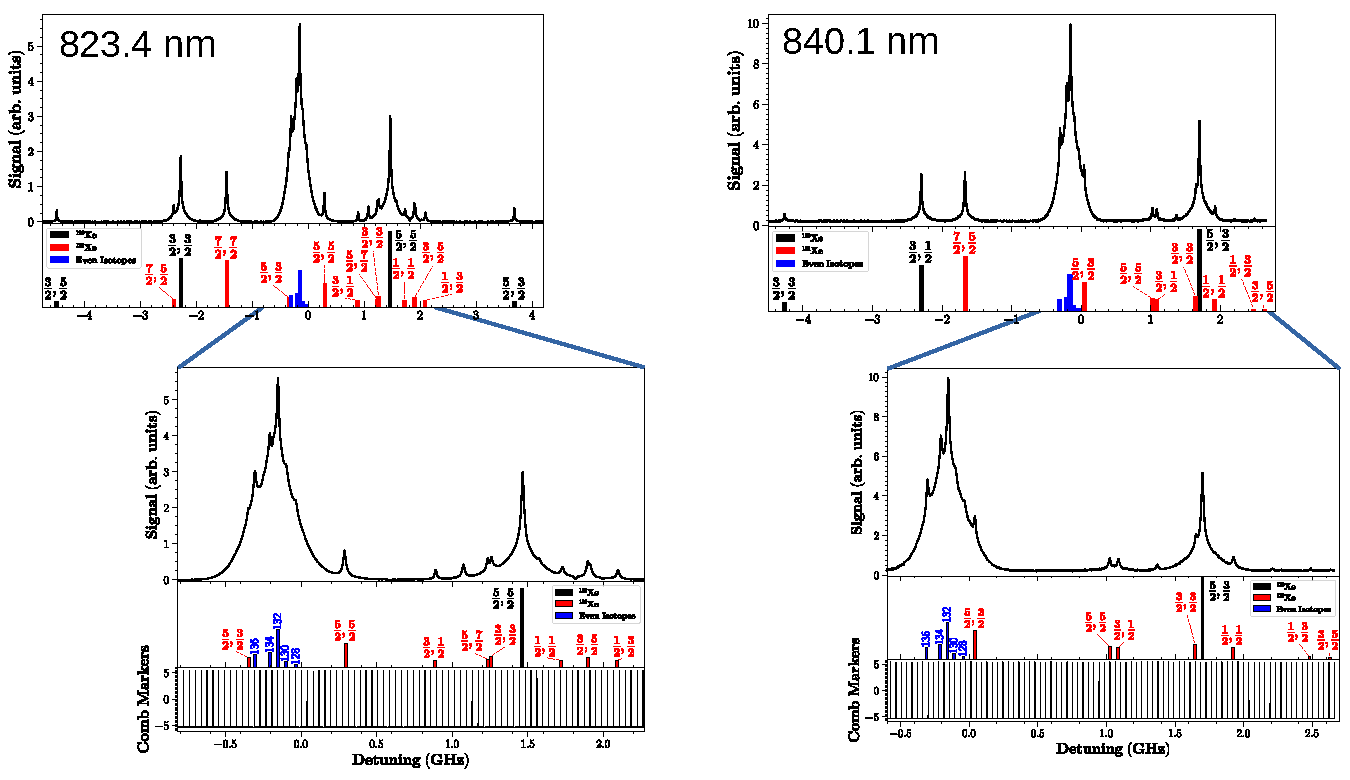
\includegraphics[width=1.0\linewidth]{diagrams/hfs_results_xeZoom}
		\caption{Experimental traces of the saturated absorption signal from the 823.1nm and 840.1nm transitions of excited xenon showing clearly resolved hyperfine peaks. The bars depict the theoretical locations of these peaks which are taken from the literature values of the hyperfine constants and isotope shifts.}
		\label{fig:hfs_resultsxezoom}
	\end{figure}
	
	\subsubsection{Isotope Shift and Hyperfine Constants -- Comparison to Literature Values} \label{sec:wl_results_Xe}
	
	The measurements presented in this section serve to provide an independent validation of the comb detuning method. It is seen from the results of Fig. \ref{fig:hfs_xelitmargs} that the comb detuning method gives hyperfine parameters with similar precision to the values published in \cite{ours_xe_paper}.
	
	We successfully extracted the hyperfine constants $A$ and $B$, as well is the isotope shift value for many transitions of xenon. This was done by fitting the experimentally measured saturated absorption curves, extracting the peak locations. Results for the isotope shift of six xenon isotopes, as well as two independent measurements of the lower state hyperfine constants, are shown in Fig. \ref{fig:hfs_xelitmargs}, where we see good agreement with other published values. These values are reflective of those published in \cite{ours_xe_paper}, with the exception of the isotope shift values for the 823nm transition. This transition was later measured using the comb calibration technique described in Sec. \ref{sec:wl_optical_detuning}. We also see the results of this measurement technique on the lower state hyperfine constants, were good self-agreement between two different transitions is seen.
	
	%The procedure which is used to extract the hyperfine constants and isotope shifts from the recorded signal will be described in detail in this dissertation.
	
	\begin{figure}[H]
		\centering
		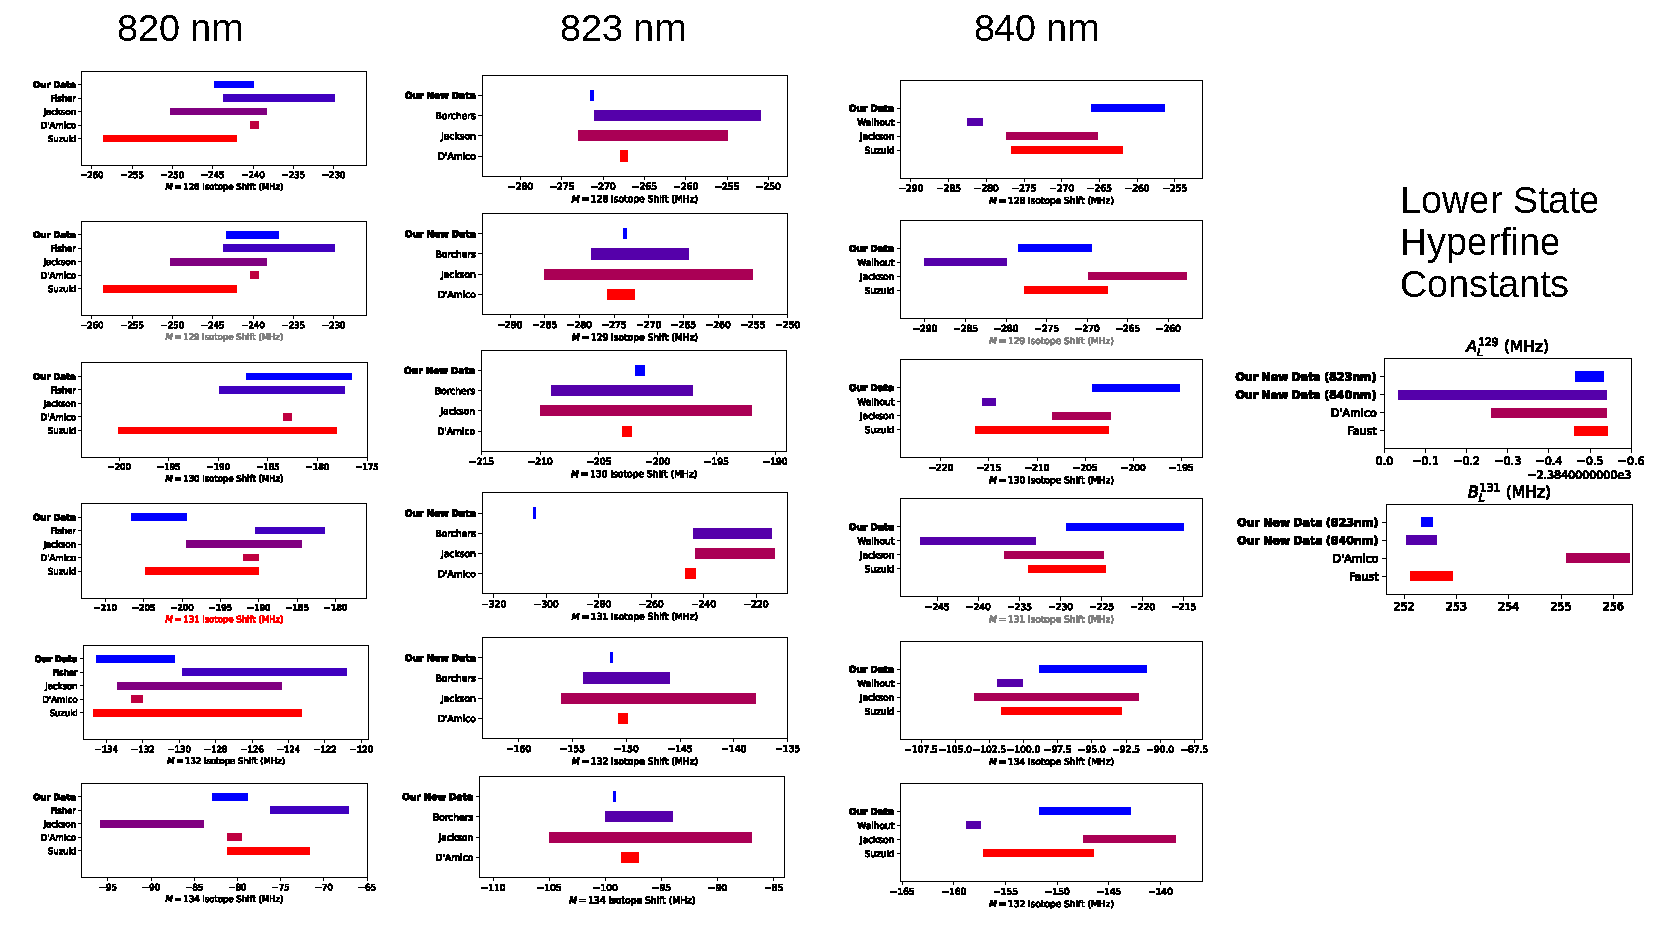
\includegraphics[width=1.0\linewidth]{diagrams/hfs_xe_litMargs}
		\caption{Isotope shift values of xenon obtained by our experiment compared to values which were obtained in the literature. The labels referring to "Our Data" refers to the data published in \cite{ours_xe_paper}, while the labels reading "Our New Data" correspond to comb calibrated measurements presented in this work.}
		\label{fig:hfs_xelitmargs}
	\end{figure}
	
	\subsection{Validation of Dynamic Wavelength Retrieval Method} \label{sec:wl_results_HFS_DWRcomb}
	In this section, we experimentally validate the DWR method by measuring the Doppler-free hyperfine spectrum of Rubidium, which provides a sharp spectral feature of known extent. This validation is performed through a simultaneous three-way measurement within a single continuous laser scan, during which we concurrently acquire the DWR reconstruction, the direct optical detuning data, and the atomic hyperfine signal. We demonstrate that the DWR method provides an accurate and independent measurement of the laser tuning, as the results show excellent agreement with the relative optical detuning method presented in Sec. \ref{sec:wl_optical_detuning}. Because the precision required for Rubidium spectroscopy is significantly more stringent than that required for breath characterization, this successful reconstruction serves as a rigorous proof-of-concept for the DWR algorithm.
	
	\begin{figure}[H]
		\centering
		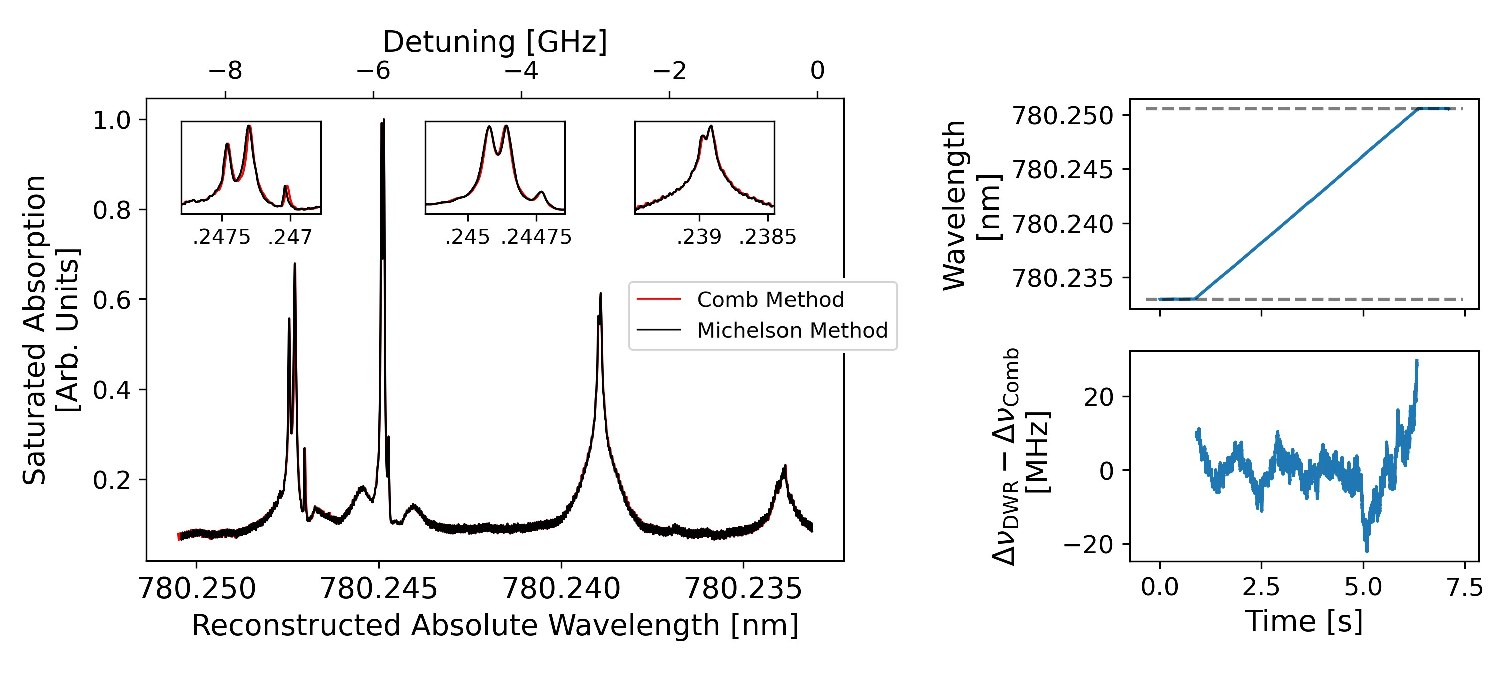
\includegraphics[width=1.0\linewidth]{diagrams/wl_comparison_combDWR}
		\caption{Measurements of the HFS of the 780.24nm (vacuum wavelength) transition in atomic Rubidium vapor. The main result is shown on the left where the saturated absorption spectrum is shown with sub-Doppler resolution. The bottom x-axis displays the absolute wavelength values recovered by the DWR method presented in Sec. \ref{sec:wl_tracking}. The top axis is the optical detuning information recovered from the comb method presented in Sec. \ref{sec:wl_optical_detuning}. Two calibrated scans are overlayed. The tight tracking is displayed by the lack of distortion of the sharp spectral features. The inset figures on the left display that absolute wavelength values for the hyperfine peaks can be obtained, which is unique for these types of measurements. The right graphs show the wavelength scan in time, and the real-time difference between the two methods, when the $\lambda(t)$ is converted into a detuning value. Throughout the scan, the tracking is within $f_\mathrm{rep}/2$, the expected precision of the comb method. The horizontal dashed lines in the upper-right wavelength plot represent the measured wavelength values used for the evaluation of the BVP.}
		\label{fig:wlcomparisoncombdwr}
	\end{figure}
	
	
%	\section{Enabling Rapid Human Breath Characterization with CW Lasers}
%	\textbf{[ \textit{We experimentally demonstrate some results here showing that the methods given in this chapter enable a class of rapid scanning CW laser-based spectrometers suitable for rapid characterization of breath samples.} ]}
%	
%	\begin{figure}[H]
%		\centering
%		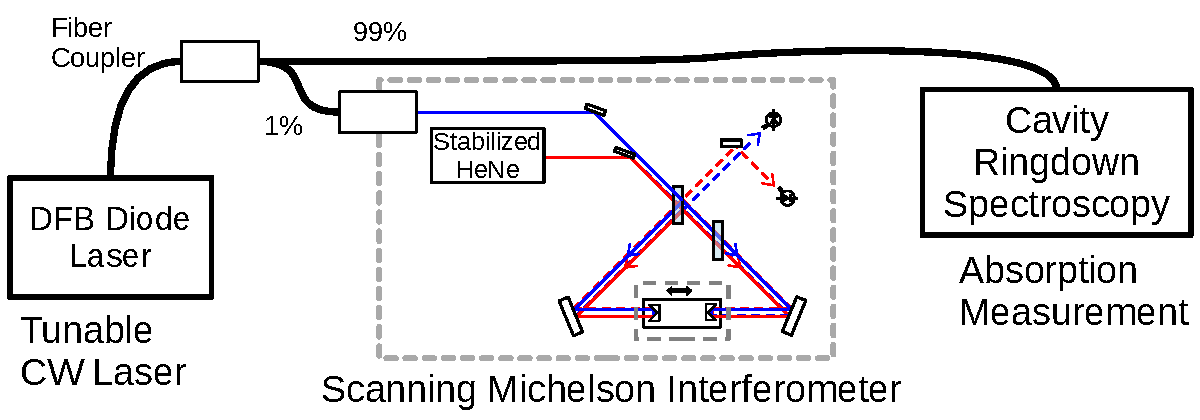
\includegraphics[width=0.8\linewidth]{diagrams/wl_crdsDemo_setup}
%		\caption{\hl{Caption Me}}
%		\label{fig:wlcrdsdemosetup}
%	\end{figure}
	
	
	\section{Summary and Conclusions}
	
	In this chapter, we have presented three complementary methods for achieving high-precision wavelength calibration in rapidly scanning continuous-wave (CW) spectroscopic systems. The central challenge addressed was the inherent trade-off between measurement speed and wavelength stability, a bottleneck that traditionally necessitates complex, hardware-intensive stabilization protocols. 
	
	We first established a foundation for precision metrology through the development of an interferometric method for extracting wavelength ratios from digital signals. By implementing interpolated phase tracking and hardware-accelerated regression on an FPGA-based platform, we demonstrated that high-resolution interferograms can be processed in real-time, effectively eliminating the data-handling bottlenecks associated with large waveform buffers.
	
	The interferometer-based Dynamic Wavelength Reconstruction (DWR) algorithm and the comb-based direct optical detuning measurements were introduced as solutions to the problem of non-stationary laser tuning. In the DWR approach, we treat the wavelength as a time-dependent variable and formulate the reconstruction as a differential tracking problem; through this method, we demonstrated that accurate spectral information can be recovered even when the laser frequency drifts significantly during a scan. Complementing this, the direct optical detuning method utilizes the dynamically changing beat note between the comb and the laser, which is converted into precise electronic markers using a filter phase-locked to the repetition rate of the comb. The robustness of these approaches was validated through rigorous testing against the hyperfine structures of Xenon and Rubidium, both of which require far greater precision than those required for breath analysis.
	
	%Finally, we demonstrated the practical utility of this method by performing rapid breath-sample measurements using an inexpensive, unstabilized DFB diode laser. This proved that high-throughput, quantitative sensing can be achieved without the need for time-consuming calibration of each scan point.
	
	While the results presented here demonstrate a significant advancement in spectroscopic capability, there remains scope for further investigation into optimizing the DWR protocol for different experimental configurations. Specifically, the performance of the algorithm could be enhanced by investigating the optimal approach to handling the initial condition of the phase evolution. In scenarios where the zero-delay point ($\delta = 0$) of the interferometer can be measured or referenced externally, the reconstruction problem could be reframed from an initial value problem into a boundary value problem. Such a transition would potentially allow for even greater suppression of systematic errors and further improve the stability of the wavelength reconstruction during long-duration scans.
	
	%\part{Fitting of Spectra}
	
	\chapter{ANALYTIC FITTING OF SPECTRA} \label{chap:fitting_spectra}
	Much of this work is concerned with quantifying the properties of gaseous substances through precise measurements of their interaction with electromagnetic radiation. In this chapter, we define the principles of absorption spectroscopy and demonstrate how these measurements relate to the intrinsic physical properties of a substance. A significant portion of this chapter is devoted to the methodology for extracting the absolute abundances of individual constituents within a gas mixture from its measured optical absorption spectrum. The ability to perform this retrieval with high accuracy is central to the development of an optical breath diagnostic platform.
	
	We present two key ideas in this chapter: the non-interacting gas approximation and the weighted linear decomposition of spectra. This leads to an approach that differs fundamentally from standard nonlinear least-squares methods, such as the Levenberg–Marquardt algorithm. Rather than iteratively linearizing the forward model about a current estimate of the parameters, we find the optimum parameters non-iteratively in a single step.
	
	The power of this explicit fitting approach is that the errors of the retrieved concentration estimates can be analyzed much more rigorously, starting from considerations of the spectral structure. Through this discussion, we give a set of formulas which directly map spectral structure, overlap, and measurement uncertainty to the fundamental precision of concentrations obtained by the fit.
	
	We conclude the discussion by presenting the self-broadening iteration, which allows the fitting procedure presented to be used in regimes where the non-interacting gas approximation fails.
	
	%It is a common task in spectroscopy to recover the concentrations of gases in a mixture from the optical absorption spectrum of the mixture.
	
	\section{The Non-Interacting Gas Approximation} \label{sec:non_interacting_gas}
	In this work, the focus is primarily on the NIR absorption spectra of gas mixtures where the primary contribution to the total pressure $P$ is from atmospheric nitrogen and oxygen. This is the regime of breath analysis, where the species of interest are present in small concentrations in a gas sample that is mostly resembling ambient air. Oxygen and nitrogen have negligible absorption contributions in the NIR range and can be essentially neglected, but the absorptions of other gas species are indirectly affected by effects such as pressure broadening.
	
	If we make the assumption that the gas samples we will be measuring will always have approximately the same content of oxygen and nitrogen, then the cross section should only depend on the total pressure $P$ and temperature $T$ of the sample. In principle the cross sections of each species can depend on the presence of other species. For instance this can occur through collision induced absorption \cite{hitran_cia_2019}. This would give rise to cross sections for each species which depend not only on the total pressure $P$ and temperature $T$, but the concentration of itself and of the other species $c_i$
	\begin{equation*}
		\sigma_i(\lambda) = \sigma_i(\lambda ;\,T, P,c_1, \ldots, c_m)
	\end{equation*}
	
	We define the non-interacting gas approximation to say that the cross-sections of the individual species are only dependent on the total temperature and pressure, assuming a gas mixture which contains mostly atmospheric nitrogen and oxygen
	\begin{equation}
		\sigma_i(\lambda ;\,T, P,c_1, \ldots, c_m) = \sigma_i(\lambda ;\,T, P)
	\end{equation}
	The cross section $\sigma_i(\lambda; T, P)$ can be thought of as the "air broadened" cross section for a dilute gas placed in an atmospheric environment.
	
	Under this assumption, the absorption coefficient of a gas mixture (\ref{alpha_mixture}) is written as a linear combination of the air broadened cross sections
	\begin{equation} \label{alpha_dilute}
		\alpha(\lambda) = \frac{P}{k_b T} \left[c_1\sigma_1(\lambda; T, P) + c_2 \sigma_2(\lambda; T, P) + \ldots \right]
	\end{equation}
	For the problem of finding a set of unknown concentrations $c_i$ by fitting an experimentally recorded spectrum, this is a great simplification. The unknown coefficients $c_i$ appear linearly in the model function, which permits least squares fitting to data using an analytic expression. This is advantageous both because there is reduced computational complexity in recovering concentrations from an absorption spectrum, but the errors of the estimates can be easily estimated. Without this simplification, iterative approaches such as the Levenberg-Marquardt algorithm must be used and require an initial guess, greatly complicating the task of a general error estimation.
	
	\section{Linear Decomposition of Spectra}
	In this section we show that the concentrations of the species in a gas mixture can be recovered from a measurement of the absorption spectrum of the mixture. 
	
	If the optical cross sections of the molecules $\sigma_j(\lambda)$ are well-tabulated for the measurement range, then we can recover the concentration values for the absorbing components in the mixture by choosing a set of $c_j$ in equation (\ref{alpha_mixture}) which reproduce the experimentally measured spectrum.
	
	Suppose we have $N$ measurements at different wavelengths $\lambda_j$ of the absorption coefficient $\alpha_j$ of a gas mixture containing a known number $m$ of gas species. From the non-interacting gas approximation (\ref{alpha_dilute}) we can write a set of $N$ equations for the absorption coefficient as the matrix multiplication
	\begin{equation} \label{fit_spectrum}
		\begin{pmatrix}
			\alpha_1 \\
			\alpha_2 \\
			\alpha_3 \\
			\vdots \\
			\alpha_N
		\end{pmatrix} =
		\frac{P}{k_B T}
		\begin{pmatrix}
			\sigma_1(\lambda_1) &  \sigma_2(\lambda_1) & \cdots & \sigma_m(\lambda_1) \\
			\sigma_1(\lambda_2) &  \sigma_2(\lambda_2) & \cdots & \sigma_m(\lambda_2) \\
			\sigma_1(\lambda_3) &  \sigma_2(\lambda_3) & \cdots & \sigma_m(\lambda_3) \\
			\vdots & \vdots& \vdots & \vdots \\
			\sigma_1(\lambda_N) & \sigma_2(\lambda_N) & \cdots &  \sigma_m(\lambda_N)
		\end{pmatrix}
		\begin{pmatrix}
			c_1 \\
			c_2 \\
			\vdots \\
			c_m
		\end{pmatrix}
	\end{equation}
	We suppose that the number of measurements is greater than the number of species present in the mixture $N > m$ which means that the system of equations above is over-determined. It is standard to use the least squares solution to such systems. We can write the above system as
	\begin{equation}
		\vec{\alpha} = A \vec{c}
	\end{equation}
	Since the set of equations is over-determined, the matrix $A$ in the above relation is not square and hence cannot be inverted. We can think of multiplying the equation above by $A^T$, which gives a new system and the solution to which is the least squares. The least squares solution to the over-determined system (\ref{fit_spectrum}) is obtained by
	\begin{equation}\label{leastSquares}
		\vec{c} = (A^T A)^{-1} A^T \vec{\alpha}
	\end{equation}
	The above solution is the choice of $c_j$ which minimizes the squared difference between the left hand side and right hand side of (\ref{alpha_mixture}) when summed over all measurements. That is the error
	\begin{align} \label{error_alpha}
		\mathrm{E}_\alpha &= \sum_{i=1}^{N} \left[\alpha_\mathrm{i} - \alpha_\mathrm{m}\left(\lambda_i\right) \right]^2 \nonumber \\ 
		&= \sum_{i=1}^{N} \left[\alpha_\mathrm{i} - \Big(n_1 \sigma_1(\lambda_i) + n_2 \sigma_2(\lambda_i) \cdots + n_m \sigma_m(\lambda_i) \Big) \right]^2
	\end{align}
	between the measured absorption values and the model predictions $\alpha_\mathrm{m}\left(\lambda_i\right)$ of (\ref{alpha_mixture}) are minimized at the measured wavelengths $\lambda_i$.
	
	In \cite{mine_acetone}, we showed that real-world concentration estimates can be improved by the use of a weighting function which minimizes bias due to the instrument response and measurement statistics. A general form for this weight function is given later in Sec. \ref{sec:weighted_fit}.
	
	\subsection{Uncertainty in the Concentration Measurement}
	From a set of absorption coefficient measurements of a gas sample having known optical cross sections of the component species, we have the explicit expression (\ref{leastSquares}) for the unknown concentrations of the species under the non-interacting gas approximation. We can use the law of propagation of errors [stats book] to obtain the uncertainty in the retrieved concentrations.
	
	From (\ref{append_leastSq_error}) and the definition $M = (A^T A)^{-1} A^T$  the deviation of the concentration of the $i^\mathrm{th}$ species is
	\begin{equation} \label{error_conc_alpha}
		\Delta {c_i} = \sqrt{\sum_j \left(M_{ij} \, \Delta {\alpha_j}\right)^2} \quad \Rightarrow \quad \Delta \alpha \sqrt{\sum_j \left(M_{ij} \right)^2}
	\end{equation}
	
	That is, the fluctuation in the concentration is calculated in terms of the fluctuation in the measured absorption. It is now clear that measurements of the absorption coefficient which are homoscedastic, where the uncertainties of all measurements is a constant $\Delta \alpha_i \Rightarrow \Delta \alpha$, then the precision of the concentration determination scales linearly with the precision of absorption coefficient determination $\Delta c_i \propto \Delta \alpha$.
	
	\subsubsection{Single Species Concentration Uncertainty}
	If we consider the specialized case of just a single species having cross section $\sigma(\lambda)$, then the matrix $A$ becomes that of a single column vector $\vec{A} = \frac{P}{k_\mathrm{B} T} \vec{\sigma}$, where $\vec{\sigma}$ is the vector having $i^\mathrm{th}$ component $\sigma(\lambda_i)$
	\begin{equation}
		\left(\vec{\sigma}\right)_i \equiv \sigma(\lambda_i)
	\end{equation}
	
	Using that $M=M_{0j}$, we have from (\ref{error_conc_alpha}) and (\ref{append_error_one_general}) the single species concentration uncertainty
	\begin{equation}\label{error_one_general}
		\Delta c = \frac{k_\mathrm{B}T}{P}\frac{1}{\vec{\sigma}\cdot\vec{\sigma}} \sqrt{\sum_j \Big(\sigma(\lambda_j) \, \Delta\alpha_j\Big)^2}
		\quad\Rightarrow\quad
		\frac{k_\mathrm{B}T}{P}\frac{\Delta \alpha}{\left|\vec{\sigma}\right|}
	\end{equation}
	
	For measurements of the absorption coefficient that have constant uncertainty $\Delta \alpha_i = \Delta \alpha$, this relation simplifies to the above right expression. If all of the $N$ measurements are conducted at a single wavelength $\lambda_i = \lambda$ where the species has cross section $\sigma = \sigma(\lambda)$, then this becomes
	\begin{equation}
		\Delta c = \frac{k_\mathrm{B} T}{P} \frac{\Delta \alpha}{\sqrt{N} \sigma}
	\end{equation}
	This gives the expected result that our uncertainty in the concentration goes as $\sim 1/\sqrt{N}$ for the measurement of a single species at a single wavelength. We see that \textit{there is no difference between averaging the absorption values at a wavelength or entering them each as separate measurements into (\ref{fit_spectrum})}.
	
	The above result is also valid for an even sampling interval of the measurement wavelengths, but we instead must make the replacement $\left|\vec{\sigma}\right| = \sqrt{\sum_i \sigma_i^2} \rightarrow \sqrt{C N}$, where the constant $C$ is related to the integral of the cross section function $\sigma(\lambda)$ over the wavelength sampling interval. Again we see the improvement in the concentration estimate going as the reciprocal square root of the number of sampled wavelengths.
	
	For an unstable laser which is used to conduct a series of measurements of absorption, it is then worthwhile to measure wavelength as often as possible during the acquisition. The efficient fringe counting procedure presented in \ref{sec:wl_wavelength} and the dynamic wavelength reconstruction method presented in \ref{sec:wl_tracking} can enable such rapid measurements with a Michelson interferometer. This allows the wavelength fluctuation of the unstable laser to be accounted for in the computation of the average absorption by entering the different wavelength-absorption measurement pairs as separate entries into (\ref{fit_spectrum}).
	
	\subsubsection{Two Species Concentration Uncertainty}
	If we have a gas mixture containing two species of interest having cross sections $\sigma_1(\lambda)$ and $\sigma_2(\lambda)$, then we have the system
	\begin{equation*}
		\vec{\alpha} =
		\underbrace{
			\frac{P}{k_B T}
			\begin{pmatrix}
				\vec{\sigma}_1 \quad \vec{\sigma}_2
			\end{pmatrix}
		}_{\begin{matrix}A\end{matrix}}
		\begin{pmatrix}
			c_1 \\
			c_2
		\end{pmatrix}
	\end{equation*}
	We define the overlap parameter $\gamma$ which measures the relative overlap of the cross sections $\sigma_1$ and $\sigma_2$
	\begin{equation}
		\gamma \equiv \frac{\vec\sigma_1\cdot\vec\sigma_2}{\sigma_1\sigma_2}
	\end{equation}
	This parameter ranges from zero to one, where a value of one means that $\sigma_1$ and $\sigma_2$ are identical up to a scale factor. In terms of the overlap parameter, the $M$ matrix is
	\begin{equation}
		M = \frac{k_\mathrm{B} T}{P} \frac{1}{1 - \gamma^2}
		\left[
		\begin{pmatrix} 1/\sigma_1^2 \\ -\gamma/\sigma_1\sigma_2 \end{pmatrix} \sigma_1^T +
		\begin{pmatrix} -\gamma/\sigma_1\sigma_2 \\ 1/\sigma_2^2 \end{pmatrix} \sigma_2^T
		\right]
	\end{equation}
	For spectra which are non-overlapping, we have orthogonality of the cross section vectors $\vec{\sigma}_1 \cdot \vec{\sigma}_2 = 0$ and the overlap parameter is zero $\gamma=0$. For many simple molecular species, the NIR cross section occurs as narrow peaks, and when these peaks are centered at different locations for the two species, the zero overlap condition is a good approximation. This gives the equivalent of (\ref{error_one_general}) for two independent single species detections when there is zero overlap between the optical cross sections in the measurement range
	\begin{equation}
		\Delta c_{i} \approxeq \frac{k_\mathrm{B} T}{P} \frac{1}{\sigma_{i}^2} \sqrt{\sum_j \left(\sigma_{i,j}\, \Delta \alpha_j\right)}
	\end{equation}
	
	For the case of constant measurement uncertainty and two species detection ($i=1,2$), equation (\ref{error_conc_alpha}) simplifies to a form given by (\ref{append_error_two_constUnc})
	\begin{equation}\label{error_two_constUnc}
		\Delta c_i = 
		\frac{k_\mathrm{B} T}{P}
		\frac{\Delta \alpha}{\left|\vec\sigma_i\right| }
		\frac{1}{\sqrt{1 - \gamma^2}}
	\end{equation}
	It is now manifest that for simultaneous measurement of two species, the \textit{minimum uncertainty in the concentrations is obtained when we have minimal overlap of the spectra}.
	
	\begin{figure}[H]
		\centering
		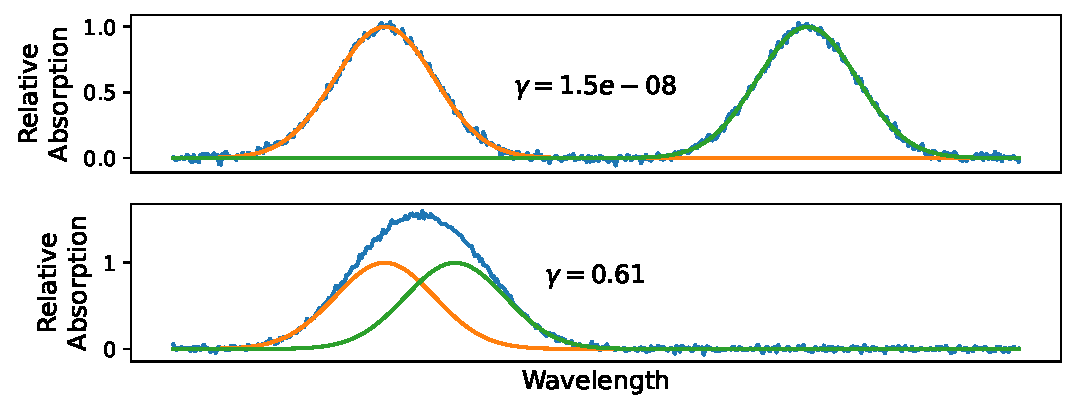
\includegraphics[width=1.0\linewidth]{diagrams/fit_overlap_twoSpec}
		\caption{Two species spectrum fitting problem shown for two extreme cases: zero spectrum overlap $\gamma \sim 0$ shown above, and large overlap $\gamma\sim 0.6$ shown below. The vertical units are proportional to the absorption coefficient $\alpha$, where the measured spectrum (shown in blue) is a linear combination of the individual absorption profiles (green and orange) for the individual species. Since the structure of the individual peaks is not resolved in the lower graph, it is then somewhat surprising that this overlap only gives a $1/\sqrt{1-\gamma^2}\sim 1.26$-fold degradation in the concentration uncertainty from the spectrum fit of the same peaks if they were isolated, given measurement noise is the same. Note that this result is independent of the relative amplitudes of the absorption features, even though they have been shown here with equal amplitudes.}
		\label{fig:fit_overlap_twospec}
	\end{figure}
	
	It can be seen in Fig. \ref{fig:fit_overlap_twospec} that even in the case of two highly overlapped spectra, concentrations can still be simultaneously determined with nearly the same precision as if the two spectral features had no overlap at all. The explicit mapping of the structure of two spectral features to a fundamental concentration uncertainty through (\ref{error_conc_alpha}), (\ref{error_one_general}), and (\ref{error_two_constUnc}) are only possible using the non-interacting gas approximation and the linear decomposition formula (\ref{leastSquares}).
	
	\subsubsection{Unresolved Baseline}
	Using as $\sigma_2(\lambda) = 1$, the corresponding vector, magnitude and overlap parameter are
	\begin{eqnarray}
		\vec{\sigma}_2 = \vec{1} &\qquad
		\sigma_2 ^2 = N &\qquad
		\gamma = \frac{\vec{\sigma}_1 \cdot \vec{\sigma}_2}{\left|\vec\sigma_1\right|\sqrt{N}} = \frac{1}{\sqrt{N}\left|\vec\sigma_1\right|}\sum_i \sigma_{1,i} \equiv \frac{\sigma_\mathrm{Avg}}{\sigma_\mathrm{RMS}}
	\end{eqnarray}
	Above we have defined the average cross section value $\sigma_\mathrm{Avg} \equiv \frac{1}{N}\sum_i \sigma_{1,i}$ and the root-mean-square cross section value $\sigma_\mathrm{RMS} \equiv \sqrt{\frac{1}{N}\sum_i \sigma_{1,i}^2} = \left|\vec\sigma_1\right|/\sqrt{N}$.
	The concentration uncertainty of the species uncertainty in baseline absorption are
	\begin{align}
		\Delta c &= \frac{k_\mathrm{B} T}{P}\frac{\Delta\alpha}{\sqrt{N}}\frac{1}{\sqrt{\sigma_\mathrm{RMS}^2 - \sigma_\mathrm{Avg}^2}} \\\nonumber\\
		\Delta B &= \frac{k_\mathrm{B} T}{P}\frac{\Delta\alpha}{\sqrt{N}}\frac{1}{\sqrt{1 - \sigma_\mathrm{Avg}^2/\sigma_\mathrm{RMS}^2}}
	\end{align}
	
	Later in Ch. \ref{chap:acetone}, we discuss fitting a near infrared spectral peak of acetone which appears to sit on top of a large broadband baseline. The above equations relate the fundamental structure of the absorption feature to the precision with which we can determine the amplitude and offset of this peak independently.
	
	\begin{figure}[H]
		\centering
		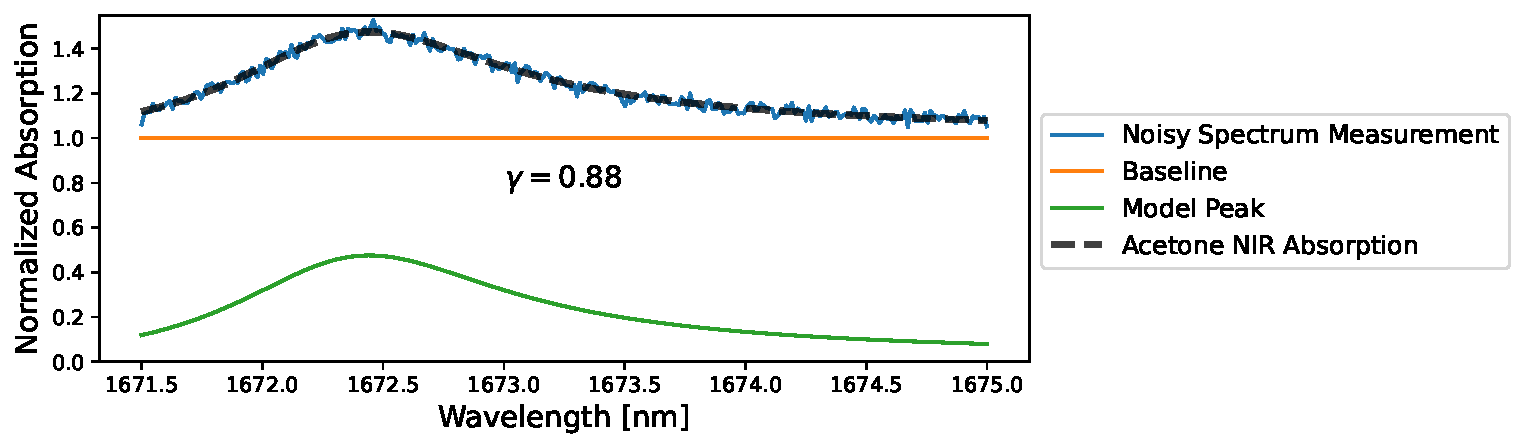
\includegraphics[width=1.0\linewidth]{diagrams/fit_overlap_acetoneBaseline}
		\caption{Determination of acetone concentration from a narrowband NIR spectrum. The overlap factor $\gamma\sim 0.88$, along with the ratio $\left|\vec{\sigma}_\mathrm{ace} + \vec{\sigma}_\mathrm{baseline}\right| / \left|\vec{\sigma}_\mathrm{ace}\right| $, gives the concentration degradation when the baseline is determined independently from the model peak amplitude. The shape of the NIR acetone absorption is determined in detail in Ch. \ref{chap:acetone}.}
		\label{fig:fitoverlapacetonebaseline}
	\end{figure}
	
	For the case of the empirically modeled acetone NIR peak given in Sec. \ref{sec:acetone_peak}, we can estimate the factor by which the precision of acetone concentration can be determined is degraded when we rely only on the peak amplitude and not the baseline information. This factor is given approximately as
	\begin{equation}
		\frac{1}{\sqrt{1-\gamma^2}} \frac{\left|\vec{\sigma}_\mathrm{acetone} + \vec{\sigma}_\mathrm{baseline}\right|}{\left|\vec{\sigma}_\mathrm{acetone}\right|} \sim 9.7
	\end{equation}
	This is computed numerically assuming an evenly spaced spectrum having a large number of points. This ratio takes into account the spectral overlap of the peak shape with the baseline, as well as the diminished effective cross section when using only the peak shape. This degradation ratio is roughly confirmed by the simulations in Sec. \ref{sec:simulation}, where a ratio of $\sim7.3$ is observed when using the weighted fit procedure.
	
	\section{Weigted Linear Decomposition} \label{sec:weighted_fit}
	
	In the previous section we showed that working in absorption units provided a particularly efficient method of fitting absorption spectra having non-interacting cross-sections. This method has the advantage that it can be performed in a single explicit step. When this is performed, the quantity in (\ref{error_alpha}) is minimized.
	
	It may be desirable to work in units other than the absorption coefficient. For instance, we may consider working in units which are the same as the measuring instrument. Suppose we have an instrument which measures a quantity $q$ which is related to the absorption coefficient through the forward model function $F(q) = \alpha(q)$. A simple example of such a function is that of (\ref{beer_absorp}) for an instrument measuring light intensities. In such a case, we can convert our theoretical absorption into a reverse model of the instrument response using the inverse function $F^{-1}(\alpha_\mathrm{m}(\lambda))$. We could then attempt to minimize the error
	\begin{align}\label{error_q}
		E_q = \sum_i \left[ q_i - F^{-1}\big(\alpha_\mathrm{m}(\lambda_i)\big) \right]^2
	\end{align}
	which would give direct agreement with the instrument measurements $q_i$ and the simulated instrument response given by $R(\alpha_\mathrm{m}\left(\lambda_i\right))$ at the wavelengths $\lambda_i$. In general the function $R(\alpha)$ is non-linear, and therefore the minimization of (\ref{error_q}) requires iterative computation.
	
	The situation may be improved by the use of a weight function. We can consider each of the terms of the sum in (\ref{error_alpha}) as representing the "closeness" of each model prediction to the measured absorption. We can multiply each equation by a constant without affecting each equality, but we may choose the constant differently for the many equations. 
	
	We denote the weight function $w(q_i)$ of the measured instrument response $q_i$ that determines the relative contribution of the terms in the sum (\ref{error_alpha}). This leads us to the weighted absorption error
	\begin{align} \label{error_weighted}
		\mathrm{E}_{\alpha,\mathrm{w}} &= \sum_{i=1}^{N} \Big[w(q_i)\alpha_\mathrm{i} - w(q_i)\alpha_\mathrm{m}\left(\lambda_i\right) \Big]^2 \nonumber \\
		&= \sum_{i=1}^{N} \Big[w(q_i)F(q_i) - w(q_i)\alpha_\mathrm{m}\left(\lambda_i\right) \Big]^2
	\end{align}
	Above we have written the measured absorption coefficient $\alpha_i$ as a function of the instrument response $\alpha_i = F(q_i)$.
	
	The sum (\ref{error_weighted}) can be minimized in a similar manner as before, but simply forming the modified $\vec{\alpha}'$ vector and $A'$ matrix
	\begin{equation} \label{fit_spectrum_weighted}
		\underbrace{\begin{pmatrix}
				F(q_1) w(q_1) \\
				F(q_2) w(q_2) \\
				F(q_3) w(q_3) \\
				\vdots \\
				F(q_N) w(q_N)
		\end{pmatrix}}_{\begin{matrix}\vec{\alpha}' \end{matrix}} % matrix for bigger underbrace text
		=
		\underbrace{\frac{P}{k_B T}
			\begin{pmatrix}
				F(q_1)\sigma_1(\lambda_1) &  F(q_1)\sigma_2(\lambda_1) & \cdots & F(q_1)\sigma_m(\lambda_1) \\
				F(q_2)\sigma_1(\lambda_2) &  F(q_2)\sigma_2(\lambda_2) & \cdots & F(q_2)\sigma_m(\lambda_2) \\
				F(q_3)\sigma_1(\lambda_3) &  F(q_3)\sigma_2(\lambda_3) & \cdots & F(q_3)\sigma_m(\lambda_3) \\
				\vdots & \vdots& \vdots & \vdots \\
				F(q_N)(\lambda_N) & F(q_N)\sigma_2(\lambda_N) & \cdots &  F(q_N)\sigma_m(\lambda_N)
		\end{pmatrix}}_{\begin{matrix} A' \end{matrix}}
		\begin{pmatrix}
			c_1 \\
			c_2 \\
			\vdots \\
			c_m
		\end{pmatrix}
	\end{equation}
	We can then find the minimum of (\ref{error_weighted}) by solving the normal equation
	\begin{equation} \label{leastSquares_weighted}
		\vec{c} = (A'^T A')^{-1}A'^T \vec{\alpha}'
	\end{equation}
	Note that the ($c_1, c_2, \ldots, c_m$) which minimize $E_{\alpha,w}$ are still found non-iteratively and analytically. This is not the case for finding the minimum of $E_q$ in (\ref{error_q}).
	
	The choice of the weight function should take into consideration the statistics of the absorption measurement uncertainty. In the next section, we propose a general method for constructing such a weight function by considering a transformation of coordinates.
	
	\subsection{A Weight Function for Linear Least-Squares Approximation of Nonlinear Models}
	
	In performing the linear decomposition of spectra (\ref{leastSquares}), we are minimizing the sum of the squared differences between the measured absorption and the model absorption given by the non-interacting gas approximation (\ref{alpha_dilute}), as shown in \ref{sec:append_linear_lsq}. It may be desirable, due to measurement statistics, to fit in the transformed space of some quantity $q$ related to absorption by a general nonlinear function. Minimizing the summed-squared error in this space usually requires a nonlinear, iterative fitting procedure. We show that the nonlinear fit in this space can be approximated by an appropriate choice of weighting function.
	
	In the following discussion, we provide a simplistic picture of the quantity $q$ as a quantity which is measured by some instrument. This quantity is related to absorption through the forward conversion $\alpha = F(q)$. This hypothetical instrument produces a measurement value of $q_0$ which corresponds to zero absorption. Although we use the language of measurement conversion for convenience, we can also think that this is some general transformation to some other coordinate, independent of whether a physical instrument is capable of directly producing such a quantity.
	
	It is possible to construct a weight function such that the coefficients $\{c_j\}$ which minimize a weighted least-squares error in weighted absorption space, $E_{\alpha,w}$, also approximately minimize the nonlinear error in the instrument response, $E_q$. This provides a means of avoiding iterative nonlinear optimization by solving a single linear least-squares problem whose objective function is constructed to mimic that of the nonlinear system.
	
	We consider a general forward model relating the instrument response $q$ to the absorption coefficient $\alpha$ through a nonlinear transformation $\alpha = F(q)$, with inverse $q = R(\alpha) = F^{-1}(\alpha)$. Let $q_0$ denote the instrument response corresponding to zero absorption, such that $F(q_0)=0$.
	
	\subsubsection{Matching Orders}
	
	The goal is to determine a weight function $w(q)$ such that the expansion of the weighted residual in absorption space,
	\begin{equation}
		E_{\alpha,w} = \sum_i \left[w(q_i)\big(\alpha_i - \alpha_{m,i}\big)\right]^2
	\end{equation}
	matches, to the highest possible order, the expansion of the residual in instrument space
	\begin{equation}
		E_q = \sum_i \left(q_i - q_{m,i}\right)^2
	\end{equation}
	Since the above expressions involve different variables, we perform the expansion about corresponding points of absorption. For the following expansions, they are performed about the points of zero absorption in their respective coordinates.
	
	Expanding the weighted residual $E_{\alpha,w}$ in absorption space about the baseline quantity $q_0$ using the forward model function $\alpha = F(q)$, we have
	\begin{align}
		E_{\alpha, \omega} &= \sum_i \Bigg\{
		-\alpha_\mathrm{m} + F'(q_0) (q_i-q_0) + \alpha_\mathrm{m}\left[1 - w(q_i)\right] \nonumber\\
		&\qquad\qquad + \frac{1}{2} \underbrace{\Big[F''(q_0) + 2 F'(q_0) w'(q_0)\Big]}_{\begin{matrix}=0\end{matrix}} (q_i-q_0)^2 \nonumber \\
		&\qquad\qquad + \frac{1}{3!}\underbrace{\Big[F'''(q_0) + 3 F'(q_0) w'(q_0) + 3F'(q_0)w''(q_0)\Big]}_{\begin{matrix}=0\end{matrix}} (q_i-q_0)^3 + \ldots
		\Bigg\}^2
	\end{align}
	This baseline measurement $q_0$ corresponds to zero absorption $\alpha_m \approx 0$. As such we perform the expansion in small model absorption $\alpha_m$. Here we make use of the reverse $R(\alpha) = F^{-1}(\alpha) = q $ mapping
	\begin{align}
		E_q &= \frac{1}{\left(F'(q_0)\right)^2} \sum_i \Bigg\{
		-\alpha_\mathrm{m} + F'(q_0)(q_i-q_0) \nonumber \\
		&\qquad\qquad\qquad + \alpha_\mathrm{m} \underbrace{\left(\frac{1}{2}\frac{F''(q_0)}{\left(F'(q_0)\right)^2}\alpha_\mathrm{m} - \frac{\frac{1}{2}\left(F''(q_0)\right)^2 - \frac{1}{6}F'(q_0) F'''(q_0)}{\left(F'(q_0)\right)^4}\alpha_\mathrm{m}^2 + \cdots\right)}_{\begin{matrix}=\left[1-w(q_i)\right]\end{matrix}}
		\Bigg\}^2
	\end{align}
	Requiring agreement order-by-order in $(q_i - q_0)$, leads to the condition that higher-order derivatives of the product $F(q)w(q)$ vanish (see Appendix B of \cite{mine_acetone}):
	\begin{equation}
		\frac{d^n}{dq^n}\big[F(q)w(q)\big] = 0, \quad n \geq 2.
	\end{equation}
	This implies that the product $F(q)w(q)$ must be linear in $q$, i.e.
	\begin{equation}
		F(q)w(q) = F'(q_0)(q - q_0)
	\end{equation}
	where the normalization $w(q_0)=1$ has been imposed. This choice of weight function is unique under the requirement that the transformed residual $F(q)w(q)$ be linear in $q$. The resulting weight function is therefore
	\begin{equation} \label{weight_function}
		w(q) = F'(q_0)\frac{q - q_0}{F(q)}
	\end{equation}
	
	This function has the useful property that the final condition of expansion order matching is approximately satisfied
	\begin{equation}
		1 - w(q_i) \approxeq \frac{1}{2}\frac{F''(q_0)}{\left(F'(q_0)\right)^2}\alpha_\mathrm{m} - \frac{\frac{1}{2}\left(F''(q_0)\right)^2 - \frac{1}{6}F'(q_0) F'''(q_0)}{\left(F'(q_0)\right)^4}\alpha_\mathrm{m}^2 + \cdots
	\end{equation}
	when we make the replacement $\alpha_m \rightarrow \alpha_\mathrm{m}(q_i)$. This replacement effectively linearizes the $E_q$ expression in the model absorption $\alpha_\mathrm{m}$, which contains the unknown scaling coefficients. This is the property that allows us to implement the linear decomposition procedure in the space of the inverse nonlinear transformation.
	
	%linearize the $E_q$ expression in $\alpha_\mathrm{m}$, and allow the linear decomposition method to work in a single step. We expect this replacement to be accurate, because if $\alpha_m$ is converging to the data up to the noise figure, then $F(q_i)$ should return a value which is close. Similarly if we operate under the assumption that this absorption value is small then its higher order discrepancies of of vanishing importance.
	
	\subsubsection{Interpretation of the Weight Function}
	This expression admits a useful interpretation in terms of the inverse function $R(\alpha)$. Using $q = R(\alpha)$, the weight may be written as
	\begin{equation}
		w(q) = F'(q_0)\frac{R(\alpha) - q_0}{\alpha}
	\end{equation}
	which corresponds to a finite-difference approximation of the inverse-function slope, normalized by the local derivative at $\alpha = 0$. In this sense, the weighting replaces the nonlinear dependence of the q-space error $E_q$ given by (\ref{error_q}) on $\alpha_m$ with a data-evaluated secant approximation, effectively linearizing the inverse mapping.
	
	
	This approach differs fundamentally from standard nonlinear least-squares methods, such as the Levenberg--Marquardt algorithm. Rather than iteratively linearizing the forward model about a current estimate of the parameters, the present method constructs a modified quadratic objective function whose residuals approximate those of the nonlinear problem. The result is a single-step linear regression that captures higher-order structure of the transformation between $q$ and $\alpha$ without requiring iteration.
	
	It is important to note that this procedure does not produce an exact equivalence to the nonlinear objective $E_q$, but rather a controlled approximation obtained by matching the expansion of the residuals about $q_0$. In practice, this reduces bias arising from the nonlinearity of $F(q)$ while retaining the computational simplicity of linear least squares.
	
	A specific instance of this general weight function was demonstrated in \cite{mine_acetone} for cavity ring-down spectroscopy (CRDS), where the transformation between a homoscedastic measurement variable (the logarithmic ring-down time) and absorption resulted in the weight function in Eq. \ref{weight_function}. The effect of this weight function on simulated spectra can be seen in Sec. \ref{sec:simulation}, where spectrum fits obtained from CRDS were seen to benefit from reduced bias in the concentration estimates.
	
	\section{Self-Broadening Iteration} \label{sec:self_broading_iteration}
	In the non-interacting gas approximation, it is assumed that there is no dependence of the cross section functions on the concentrations of the species, $\sigma_i(\lambda ;\,T, P, c_1, \ldots, c_m) \rightarrow \sigma_i(\lambda ;\,T, P)$. In the next chapter, line broadening mechanisms will be discussed. Among the most important broadening mechanisms for modeling gases near ambient pressure is collisional broadening. Such a broadening mechanism gives such a dependence of the cross section functions on the concentrations $c_1 \ldots c_m$ of all species.
	
	To handle such cases, we may first assume that the main contribution to the total gas pressure $P$ is from atmospheric nitrogen and oxygen. Even in a breath sample rich with water vapor and carbon dioxide, O$_2$ and N$_2$ still form the bulk of the gas particles. It is therefore reasonable to assume that the dependence of the cross section functions on the concentrations is weak enough that the assumption of a "dry air mixture" is sufficient to give a good approximation for the effects of collisional broadening.
	
	This observation allows us to motivate the self-broadening iteration. First, the cross section functions are calculated under the assumption of a dry air mixture and the non-interacting gas approximation. This already gives a reasonable approximation to the concentrations of the gas species using the linear decomposition formula (\ref{leastSquares}). From these concentration values, we can then update the cross section functions $\sigma_i(\lambda ;\,T, P, c_1, \ldots, c_m)$ using their known dependence on $c_1 \ldots c_m$.
	
	Some details of the calculation of cross section functions will be discussed in Ch. \ref{chap:lineshapes}. The primary effect causing a difference between the cross sections appearing in a dry air mixture and those of a gas mixture containing other species is self-broadening. This effect is most prominent for water and carbon dioxide, since their concentrations in breath samples can reach several percent. This level of change in the composition of the broadening environment becomes perceptible in the spectroscopic lineshape. While there are cross-collisional effects \cite{hitran_cia_2019}, they tend to be weaker and not as well documented as self-broadening effects.
	
	\begin{figure}[H]
		\centering
		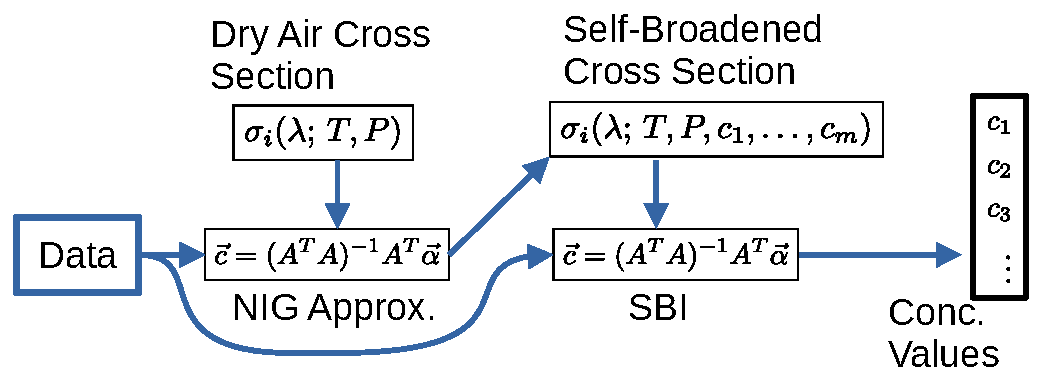
\includegraphics[width=0.85\linewidth]{diagrams/fit_SBI_flow}
		\caption{Flowchart of the self-broadening iteration. The data is first fit using (\ref{leastSquares}) under the non-interacting gas approximation (NIG). The cross sections used for the computation are assumed to be those of a dilute dry air mixture. The resulting concentration values are then used to update the cross section models, including self-broadening effects, and these are used to obtain a final set of concentration values through a second application of (\ref{leastSquares})}
		\label{fig:fit_sbi_flow}
	\end{figure}
	
	\begin{figure}[H]
		\centering
		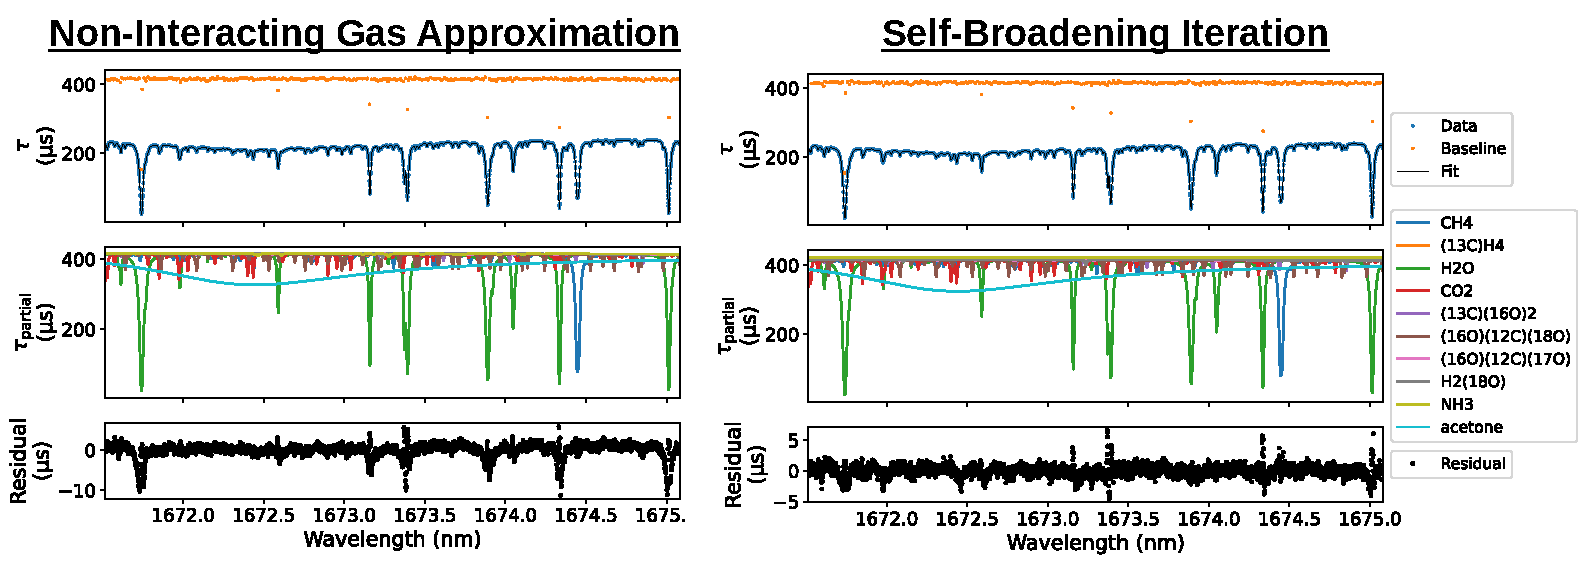
\includegraphics[width=1.0\linewidth]{diagrams/fit_SBI_results}
		\caption{The effect of the self-broadening iteration is shown for fitting cavity ringdown spectroscopy (CRDS) data. The vertical axis on the top and middle plots is the ringdown time, which is reciprocally related to absorption (see Ch. \ref{chap:CRDS}). It can be seen from the residual plots in the lower panes (constructed by subtracting the data from the fit curve) that the self-broadening iteration noticeably improves the fit residuals.}
		\label{fig:fit_sbi_results}
	\end{figure}	
	
	\chapter{DESCRIPTION OF ABSORPTION LINESHAPES}\label{chap:lineshapes}

	\section{Quantum Mechanical Description of Light Interaction}
	In the presence of an electromagnetic field, the Hamiltonian for a particle of charge $q$ under the influence of the scalar potential $\phi$ and vector potential $\Avec$ is given by:
	$$H = \frac{1}{2m}(\vec{\mathbf{p}} - q\Avec)^2 + q \phi$$
	By applying a gauge transformation of the wavefunction phase $\psi'(\rvec,t) = \psi(\rvec,t)\exp[i\chi(\rvec,t)/\hbar]$, where the gauge function is defined as $\chi(\rvec,t) = \frac{q}{e}\Avec \cdot \rvec$, we can transition from the velocity gauge to the length gauge ($\Avec'=0$). In this gauge, the interaction Hamiltonian $H_\mathrm{int}$ is expressed via the coupling of the electric dipole operator $\vec{\mathbf{D}} = - e\rvec$ to the electric field $\vec{\mathbf{E}}(t) = \mathcal{E}(t)\hat{\epsilon}$, giving the transition strength as the projection of the transition dipole operator $\vec{\mathbf{D}}$ onto the polarization direction $\mathbf{\hat{\epsilon}}$
	\begin{equation} \label{interaction_hamiltonian}
		H_\mathrm{int} = -\mathbf{\hat{\epsilon}} \cdot \vec{\mathbf{D}} \mathcal{E}(t)
	\end{equation}
	The strength of a transition from an initial state $|a\rangle$ to a final state $|b\rangle$ is governed by the vector-valued matrix element
	\begin{align}\label{dipoleElement}
		\vec{\mathbf{D}}_{ba} = \langle b|\vec{\mathbf{D}}|a\rangle
		&= -e\int\psi_b^*(\rvec)\rvec\psi_a(\rvec)d\rvec \nonumber\\
		&= -e \left[ \left( \int \psi_b^* x \psi_a \, d^3\mathbf{r} \right) \mathbf{\hat{i}} + \left( \int \psi_b^* y \psi_a \, d^3\mathbf{r} \right) \mathbf{\hat{j}} + \left( \int \psi_b^* z \psi_a \, d^3\mathbf{r} \right) \mathbf{\hat{k}} \right]
	\end{align}
	
	The physical consequence of this matrix element on observable properties of transitions is manifest through the Einstein $A$ and $B$ coefficients, which are linked to the dipole matrix element via	
	\begin{equation} \label{einstein_link}
		B_{ba} = \frac{\pi}{3\hbar^2 \epsilon_0} \left| \vec{\mathbf{D}}_{ba} \right|^2,
		\qquad\qquad
		A_{ba} = \frac{\omega_{ba}^3}{3\pi c^3 \hbar \epsilon_0} \left| \vec{\mathbf{D}}_{ba} \right|^2,
	\end{equation}
	together with the thermodynamic detailed balance relation
	\begin{equation} \label{einstein_balance}
		A_{ba} = \frac{8\pi h \nu^3}{c^3} B_{ba}.
	\end{equation}
	These relations ensure that, in thermal equilibrium, the net population flow between the two states vanishes when radiative processes are balanced against the spectral energy density of the radiation field.
	
	The practical utility of these coefficients is realized through the Füchtbauer–Ladenburg relation, which connects the spontaneous emission rate to measurable spectroscopic quantities. Consider a beam of radiation with spectral intensity $I_\nu$ propagating through a thin layer of atoms (see discussion surrounding Fig. \ref{fig:absorption_prop}), where the rate of change in intensity $d\left[I_{\nu}d\nu\right] / dx$ over a narrow spectral range of extent $d\nu$ is proportional to the difference between absorption and stimulated emission processes. Since the Einstein coefficients are defined in terms of the spectral energy density $\rho(\nu)$, related to intensity by $\rho(\nu) = I_\nu / c$, the microscopic gain/loss form of the radiative transfer equation is
	\begin{equation}
		-\frac{d I_\nu}{dx} = \frac{h\nu}{c} \left( B_{ab} N_a - B_{ba} N_b \right) \ell(\nu)
	\end{equation}	
	where $N_a$ and $N_b$ are the populations of the upper and lower states, and $\ell(\nu)$ is the normalized lineshape function satisfying $\int \ell(\nu) \, d\nu = 1$, which distributes the transition probability over frequency. Upon integration, we may assume the lineshape $\ell(\nu)$ is sufficiently narrow such that the frequency dependence of the pre-factors can be approximated by the line center frequency, $\int \nu \ell(\mathbf{\nu}) \, d\nu \approx \nu_0$.
	
	Identifying the absorption coefficient via $\alpha(\nu) = -\frac{1}{I_\nu}\frac{dI_\nu}{dx}$, and integrating over the spectral line (asuuming a narrow linewidth so that $\nu \approx \nu_0$ within the integral), we obtain the radiative transfer equation
	\begin{equation}
		\int \alpha(\nu)\,d\nu
		= \frac{h}{c} \left( B_{ab} N_a - B_{ba} N_b \right) \int \ell(\nu) \nu \, d\nu
		= \frac{c^2}{8\pi \nu_0^2} A_{ba} \left( N_a - \frac{g_a}{g_b} N_b \right)
	\end{equation}
	Above we have used the degeneracy relation $g_a B_{ab} = g_b B_{ba}$ and the detailed balance relation (\ref{einstein_balance}).
	
	A particularly important limiting case arises when the upper-state population is negligible $(N_b \ll N_a)$, for which the absorption coefficient is directly proportional to the absorption cross section $\sigma_a(\nu)$ via $\alpha(\nu) = N_a \sigma_a(\nu)$. In contrast, the Füchtbauer–Ladenburg relation is most naturally expressed in terms of the emission cross section $\sigma_e(\nu)$, for which the dependence on population cancels. In this case, one obtains
	\begin{equation}
		\int \nu^2 \sigma_e(\nu)\, d\nu = \frac{A_{ba} c^2}{8\pi}
	\end{equation}
	which provides a direct connection between the spontaneous emission rate and the integrated emission cross section. This relation forms the basis for reconstructing emission cross sections from spectroscopic data and underlies the structure of some tabulated transition probabilities \cite{lineshapes_fuchtbauer_laden}.
	
	\section{Models of Absorption Lineshapes}
	Spectroscopy is an indispensable tool for probing fundamental physical phenomena, as atomic and molecular spectra provide a direct measure of energy differences between quantum mechanical states. However, experimental observations rarely involve single, isolated atoms. Although transition frequencies of individual atoms have been measured under highly controlled trapping conditions (see \cite{ours_single_mg_comb_line}), the present work focuses on spectra observed under standard laboratory conditions. To achieve an accurate description of realistic absorption lineshapes, it is necessary to account for three primary broadening mechanisms: Doppler broadening due to the thermal motion of the absorbing species, natural broadening arising from the finite lifetime of the excited state, and pressure broadening resulting from collisions between gas particles.
	
	The fundamental description of light absorption in atoms and molecules is intrinsically linked to their emission-related processes, a consequence of thermodynamic consistency and the principle of detailed balance as expressed via the Einstein $A$ and $B$ coefficients in (\ref{einstein_balance}). Consequently, for the purposes of this discussion, we treat absorption and emission as a unified phenomenon.
	
	According to the Wiener-Khinchin theorem, the time-averaged radiated power spectrum $P_{\text{av}}(\omega)$ is proportional to the Fourier transform of this correlation function \cite{book_born_and_wolf_princpOptics}
	\begin{equation}
		I(\omega) \propto \left| \int_{0}^{\infty} \langle \hat{d}^\dagger(t)\hat{d}(0) \rangle e^{i\omega t} dt \right|^2
	\end{equation}
	
	%Consider a beam of radiation with intensity $I_\nu$ propagating through a thin layer of atoms, where the rate of change in intensity $I(\nu)$ is proportional (see discussion surrounding Fig. \ref{fig:absorption_prop}) to the difference between absorption and stimulated emission rates. These atoms are described by a density $N_a$ in the lower state and $N_b$ in the upper state. The rate of energy attenuation through an infinitesimal slab of thickness $dx$ is determined by the difference between the rates of absorption and stimulated emission
%	\begin{equation}
	%		-\frac{d(I_\nu d\nu)}{dx} = \frac{h\nu}{c} \left( B_{ab} \,dN_{a,\nu} - B_{ba} \,dN_{b,\nu} \right)
	%	\end{equation}
	%where $n$ is the refractive index of the medium.
	
	%By relating this attenuation to the absorption coefficient obtained in Eq. (\ref{beer_absorp}) for $\alpha(\nu)$, where $\alpha(\nu)d\nu = -\frac{1}{I_\nu}\frac{dI}{dx}d\nu$, and integrating over the full spectral line, we arrive at the relation
%	\begin{equation}
%		\int \alpha(\nu)\,d\nu = \frac{h\nu_0}{c} \left( B_{ab}N_a - B_{ba}N_b \right) = \frac{c^2 A_{ba}}{8\pi \nu_0^2}\left( N_1 - \frac{g_1}{g_2}N_2 \right)
%	\end{equation}
%	This relation provides the direct link between the spontaneous emission rate $A_{ba}$ and the integrated absorption cross-section used to reconstruct the spectra from the HITRAN database. Putting in terms of the optical frequency and optical cross section $\sigma(\nu)$, we have
%	\begin{equation}
%		\int \nu^2 \sigma (\nu) d\nu = \frac{A_{ba} c^2}{8\pi n^2}
%	\end{equation}
	
	\subsection{Natural Lineshape}
	In the absence of vacuum fluctuations and coupling to a thermal reservoir, standard quantum mechanics predicts that excited states are stationary and persist indefinitely without decay. While a complete description of spontaneous emission requires the framework of Quantum Electrodynamics (QED) to account for the interaction between the atom and the electromagnetic vacuum, a phenomenological approach is sufficient to model the absorption lineshape produced by such an excited state transition.
	
	By treating the excited state as having a finite lifetime $T$, the dipole correlation function can be modeled as a decaying exponential. This approximation is mathematically sufficient for describing the resulting Lorentzian lineshape, and it establishes the necessary link between fundamental quantum transitions and the empirical line strengths ($S_{ij}$) utilized in the computational models for spectroscopic databases.
	
	The lifetime $T$ of the excited state is fundamentally linked to the spontaneous emission coefficient $A_{ba}$ via the relation $\gamma = 1/T \propto A_{ba}$, resulting in a spectral linewidth $\Delta \nu$ dictated by the energy-time uncertainty principle $\Delta E \Delta t = (h\Delta \nu) T = \hbar /2$. By modeling the decay of the dipole correlation function as an exponential process, we arrive at the characteristic Lorentzian lineshape after performing the Fourier transform
	\begin{align}
		I(\omega) \propto& \int_{0}^{\infty} e^{i (\omega - \omega_0)t} e^{-\gamma t / 2} dt \nonumber\\
		&= \frac{1}{\gamma /2 - i(\omega - \omega_0)} = \frac{\gamma /2 - i(\omega - \omega_0)}{(\omega - \omega_0)^2 + \gamma^2 /4}
	\end{align}
	The absorption coefficient is determined by the real part of this expression \cite{book_molecules_and_radiation}, which results in a Lorentzian lineshape:
	\begin{equation} \label{ls_lorentzian}
		l_\gamma(\omega) = l_0 \frac{\gamma}{(\omega - \omega_0)^2 + \gamma^2/4}
	\end{equation}
	where $\gamma$ represents the decay rate.
	
	Even in the absence of thermal motion or Doppler broadening, this intrinsic natural lineshape persists. This result represents the fundamental limit of homogeneous broadening, which is a regime where every constituent atom or molecule in the ensemble shares the same transition frequency and linewidth. Because this lineshape arises solely from the intrinsic lifetime of the excited state rather than external environmental fluctuations, it is referred to as the natural lineshape. This functional form is characteristic of any system governed by an exponentially decaying dipole correlation function, and it appears frequently across various physical contexts \cite{book_foot2005atomic, book_fourier}.
	
	\subsection{Doppler Broadening}
	The most prominent source of inhomogeneous broadening in gas-phase spectroscopy is the thermal motion of the absorbing species. According to the Doppler effect, an atom moving with a velocity component $v_z$ along the line of $\text{sight}$ of the radiation beam will perceive the frequency of the incident light as being shifted by $\Delta \omega = \omega_0 (v_z/c)$. 
	
	In a system in thermal equilibrium at temperature $T$, the velocities of the particles follow a Maxwell-Boltzmann distribution, and the probability density for a velocity component $v_z$ is given by:
	\begin{equation}
		P(v_z) = \sqrt{\frac{M}{2\pi k_B T}} \exp\left( -\frac{M v_z^2}{2 k_B T} \right)
	\end{equation}
	where $M$ is the mass of the particle and $k_B$ is the Boltzmann constant. By mapping this velocity distribution onto the frequency domain via the Doppler shift relation, we obtain a Gaussian lineshape:
	\begin{equation} \label{ls_doppler}
		g(\omega) = \frac{1}{\sigma \sqrt{2\pi}} \exp\left( -\frac{(\omega - \omega_0)^2}{2\sigma^2} \right)
	\end{equation}
	where the standard deviation $\sigma$ is proportional to $\sqrt{T/M}$. Unlike the natural lineshape, which is a homogeneous broadening mechanism, Doppler broadening is fundamentally inhomogeneous, as each molecule in the ensemble possesses a different central frequency determined by its individual velocity vector. Consequently, as temperature increases or molecular mass decreases, the spectral line undergoes significant broadening, and the wings of the profile decay much more rapidly than those of a Lorentzian profile.
	
	\subsection{Pressure (Collisional) Broadening}
	While Doppler broadening arises from the motion of the particles, collisional broadening arises from the interaction between them. In a high-pressure environment, the time between successive collisions, $\tau_c$, becomes significantly shorter than the natural lifetime $T$. Each collision event can be viewed as a stochastic interruption of the phase coherence of the radiating dipole, which effectively resets the decay process.
	
	Mathematically, this is equivalent to adding an additional exponential decay term to the dipole correlation function. If we denote the collision rate as $\gamma_{\text{coll}} = 1/\tau_c$, the total decay rate becomes $\Gamma = \gamma_{\text{nat}} + \gamma_{\text{coll}}$. As demonstrated in the derivation of the natural lineshape, any process that introduces an exponential decay into the correlation function results in a Lorentzian profile. Thus, pressure broadening retains the functional form of a Lorentzian but with an increased Full Width at Half Maximum (FWHM) \cite{book_lasers_siegman}. This effect is particularly dominant in high-density gases where the collision frequency $\gamma_{\text{coll}}$ exceeds the natural decay rate $\gamma$.
	
	\subsection{The Voigt Profile}
	In practical laboratory spectroscopy, particularly when analyzing gas-phase molecules at room temperature and moderate pressures, the observed spectral profile is shaped by both Doppler broadening and collisional or natural broadening. Because these two broadening processes are statistically independent, the resulting lineshape is mathematically described by the convolution of a Gaussian profile and a Lorentzian profile. This convolution, known as the Voigt profile, $V(\omega)$, is defined as:
	\begin{equation}
		V(\omega; \sigma, \gamma) = (g * l)(\omega) = \int_{-\infty}^{\infty} g_\sigma(\omega') l_\gamma(\omega - \omega') d\omega'
	\end{equation}
	The Voigt profile effectively captures the physics of both broadening regimes, as it retains a Gaussian core dominated by thermal motion while exhibiting the characteristic power-law Lorentzian wings resulting from pressure and lifetime broadening. In the cases where $\sigma=0$ or $\gamma=0$, the Voigt profile reduces to a Lorentzian and a Gaussian, respectively, and in effect, it interpolates between the two profiles. Although the Voigt profile lacks a closed-form analytical solution in terms of elementary functions, it can be computed efficiently via the Faddeeva function, which is essential for implementing scalable nonlinear least-squares fitting routines.
	
	Accurately modeling the transition between the Doppler-limited and pressure-broadened regimes is essential for the precise extraction of molecular parameters from experimental spectra. Under many common experimental conditions, the Voigt profile provides a sufficient description of the observed line shapes for isolated transitions where spectral congestion is minimal.
	
	\subsection{Modern Descriptions of Lineshapes and Spectroscopic Databases}
	While the Voigt profile serves as a robust approximation for many spectroscopic applications, it fails to capture subtle physical phenomena that become critical during high-precision measurements. In the context of trace gas sensing or atmospheric remote sensing, even minute deviations from the convolution of Gaussian and Lorentzian profiles can introduce significant systematic errors in the retrieval of molecular concentrations or temperatures.
	
	As spectroscopic precision has advanced toward the sub-Doppler limit, more sophisticated models have been developed to account for the complex dynamics of molecular interactions \cite{book_collisionalEffects_hartmann}. For instance, at high pressures or in the presence of strong external fields, the assumption of a simple additive decay rate breaks down. Advanced models must account for speed-dependent effects, where the impact of collisions depends on the velocity of the absorbing species; this effectively couples the Doppler and pressure broadening mechanisms in a way that the standard Voigt profile cannot. This necessitates more rigorous profiles, such as the Speed-Dependent Voigt (SDV) or the Hartmann-Tran profile \cite{hartmann_tran_IUPAC}, which explicitly account for the correlation between velocity and collision frequency.
	
	These advanced, physically motivated lineshapes form the backbone of modern spectroscopic databases, such as HITRAN (High-resolution Transmission molecular absorption database) and GEISA (Gestion Électronique des Spectres d'Absorption). Rather than storing raw experimental spectra, these databases provide a structured collection of fundamental molecular parameters, including line centers, intensities, and broadening coefficients. These parameters can subsequently be used to reconstruct the absorption spectrum under arbitrary temperature and pressure conditions using the aforementioned models. The construction of such databases relies on the systematic extraction of these parameters from high-resolution experimental or theoretical datasets.
	
	By utilizing advanced lineshape models, these databases enable the "forward modeling" of synthetic spectra by coupling fundamental molecular parameters with physically appropriate profiles (e.g., SDV) tailored to specific experimental conditions. This capability is essential for the high-accuracy retrieval of atmospheric constituents from satellite-based infrared spectrometers; in such applications, accounting for subtle deviations from a standard Voigt profile often represents the difference between a successful detection and an uninterpretable signal \cite{hitran_cia_2019}.
	
	\subsection{The HITRAN Database}
	
	Throughout this work, we will make frequent comparisons between measured spectra and simulated absorptions using parameters from the HITRAN database. Although software packages exist to readily compute absorption curves using these parameters, such as the HAPI interface \cite{HAPI_2016}, we discuss some of the details of the database and how absorption curves are derived from it.
	
	Historically, the HITRAN database began as a minimal, deliberately compact, and machine-parsable repository containing only the essential parameters required to compute Voigt profiles for transitions relevant to atmospheric transmission \cite{hitran_original_1973}. For every transition recorded in HITRAN, a set of empirically determined spectroscopic constants is provided, accompanied by literature references from which they were derived. By utilizing these constants within appropriate lineshape models, the absorption coefficient as a function of wavelength can be reconstructed.
	
	Over time, the database structure has evolved to include parameters describing more advanced lineshape behaviors \cite{hitran_1986}, eventually transitioning to the Hartmann-Tran (HT) profile, which became the recommended profile with the release of HITRAN 2016 \cite{hitran_2016}, remaining with the most recent release \cite{hitran_2024}. In a manner analogous to how the Voigt profile can be reduced to either a Lorentzian or a Gaussian, the parameters provided in the HITRAN database for HT profile modeling are sufficiently comprehensive to allow for the computation of simpler models, such as the Voigt profile. Specifically, by setting higher-order coefficients to zero, such as those representing speed-dependence and collision-induced frequency shifts, the model simplifies back to the standard Voigt regime. This hierarchical structure allows researchers to scale the computational complexity of the lineshape model according to the specific precision requirements of their application.
	
	Despite the availability of an extended parameter set within HITRAN, the spectroscopic data for the 1.6–1.7 {\textmu}m region, a relevant window for breath analysis, remains incomplete. For key species such as methane ($\text{CH}_4$), water vapor ($\text{H}_2\text{O}$), and carbon dioxide ($\text{CO}_2$), modern experimental techniques, including dual-comb and cavity ring-down spectroscopy, have clearly demonstrated the necessity of modeling effects beyond the Voigt approximation, such as speed-dependence and Dicke narrowing. However, these advanced parameters are currently available for only a limited subset of transitions and are typically derived under simplified conditions, such as pure-gas or air-broadening regimes. In realistic breath mixtures, where $\text{CH}_4$ interacts with significant concentrations of $\text{CO}_2$ and $\text{H}_2\text{O}$, the collisional environment is both compositionally complex and strongly perturber-dependent, necessitating distinct parameter sets for each absorber–perturber pair. At present, beyond-Voigt parameterizations for cross-species interactions are sparse, non-systematic, and frequently absent. Consequently, high-precision modeling in this region often relies on Voigt or partially corrected profiles, where effective parameters must absorb unresolved physics, thereby limiting both the accuracy and the transferability of spectroscopic retrievals in breath analysis applications.
	
	Resolving these deficiencies requires a systematic expansion of spectroscopic databases through targeted experimental campaigns. Future work on this front must focus on high-resolution, pressure-dependent spectroscopic sweeps conducted under controlled temperature ranges to isolate the specific contributions of cross-species collisions. Such studies are necessary to characterize the individual collision-induced frequency shifts and speed-dependence coefficients for each absorber–perturber pair, which will facilitate a transition from empirical, effective parameters toward a fundamentally accurate description of the collisional environment in complex mixtures.
	
	Not all transitions, especially the broad absorption bands created by complex molecules, can be effectively modeled using line-by-line parameters. This work helps to address the deficiency of NIR spectroscopic references for gaseous acetone, one of the most important breath biomarkers. In Sec. \ref{sec:acetone_broadband}, we present an empirical model of the acetone NIR absorption cross section, constituting the highest resolution model of this absorption published to date.
	
	\subsubsection{HITRAN Voigt Profile Parameters}
	Although it is possible to compute the full Hartmann-Tran profile for many species relevant to breath analysis using the parameters in the HITRAN database, many of the empirical higher order terms necessary to fully describe the interactions between species have not been resolved to enable this level of accuracy. As such, we must revert back to the Voigt profile computation for many species. We give here a description of the minimum parameters necessary to compute an accurate Voigt profile from the HITRAN database, along with the notation used in the official documentation
	
	\begin{itemize}
		\item \textbf{Line Center ($\nu_{ij}$):} [$\text{cm}^{-1}$] The frequency of the center of the molecular transition, provided in wavenumbers.
		\item \textbf{Line Intensity at Reference Conditions ($S_{ij}$):} [$\text{cm}^{-1}$] The integrated absorption cross-section of the transition at a reference temperature of $T_\mathrm{ref} = 296$ K and a reference pressure of $P=1$ atm. This quantity is weighted by terrestrial isotopic abundances, and this scaling must be undone for isotopic analysis. For other temperatures, the line intensity must be computed. For a transition between two rovibronic states, the spectral line intensity is given as
		\begin{equation}\label{hitran_S}
			S_{ij} = I_a \frac{A_{ji}}{8\pi c \nu_{ij}^2}\frac{g' e^{-c_2E''/T} \left(1-e^{-c_2\nu_{ij} /T}\right)}{Q(T)}
		\end{equation}
		where $A_{ji}$ [s$^{-1}$] is the Einstein coefficient of spontaneous emission, $g'$ is the upper statistical weight, and $E'' = E_i$ is the lower state energy [cm$^{-1}$]. The term $Q(T)$ is the total internal partition sum
		\begin{equation}
			Q(T) = \sum_k g_k \exp\left(-\frac{c_2 E_k}{T}\right)
		\end{equation}
		%\item \textbf{Einstein-A Coefficient ($A_{ji}$):} [s$^{-1}$] The Einstein-A coefficient of spontaneous emission. This parameter was chosen as a line descriptor after the introduction of the 160-character ".par" format used for the HITRAN 2004 database \cite{hitran_2004}, since it is independent of the type of transition (electric dipole, electric quadrupole, magnetic dipole, etc.)
		\item \textbf{Air-Broadening Coefficient ($\gamma_{\mathrm{air}}$):} [cm$^{-1}$/atm] The air-broadened HWHM at $T_\mathrm{ref} = 296$ K and reference pressure $P_\mathrm{ref} = 1$ atm
		\item \textbf{Self-Broadening Coefficient ($\gamma_\mathrm{self}$):} [cm$^{-1}$/atm] The self-broadened HWHM at $T_\mathrm{ref} = 296$ K and reference pressure $P_\mathrm{ref} = 1$ atm
		\item \textbf{Temperature-Scaling Exponent ($n_\mathrm{air}$):} The exponent used to quantify the temperature dependence of the pressure-broadening coefficients $\gamma_\mathrm{air}$ and $\gamma_\mathrm{self}$.
		\item \textbf{Pressure-Shift Coefficient ($\delta_{\text{air}}$):} [cm$^{-1}$/atm] The coefficient describing the frequency displacement (shift) of the line center as a function of the partial pressure of air. Can be positive or negative.
		\item \textbf{Lower-State Energy of the Transition ($E''$):} [cm$^{-1}$] Defined with a zero point corresponding to the lowest energy state of the particular isotopologue
		\item \textbf{Doppler Width Parameter ($\gamma_D$):} The Gaussian component of the profile, which is determined by the molecular mass and the kinetic temperature of the gas species (see Eq. (\ref{ls_doppler})).
		\item \textbf{Lower and Upper Statistical Weights ($g''$ and $g'$):} Includes electronic, vibrational, rotational, and nuclear statistics. Their computation is explained in \cite{hitran_statistical_weights}
	\end{itemize}
	
	The HWHM of the pressure-broadened Lorentzian component at total pressure $P$ [atm], temperature $T$ [K] and partial pressure $p_\mathrm{self}$ [atm] is modeled by
	\begin{equation}
		\gamma(P, T) = \left(\frac{T_\mathrm{ref}}{T}\right)^{n_\mathrm{air}} \Big[
		\gamma_\mathrm{air}(P_\mathrm{ref}, T_\mathrm{ref}) \left(P - p_\mathrm{self}\right) +
		\gamma_\mathrm{self}(P_\mathrm{ref}, T_\mathrm{ref}) p_\mathrm{self}
		\Big]
	\end{equation}
	The pressures shift of the line position gives the new line position
	\begin{equation}
		\nu^*_{ij} = \nu_{ij} + \delta(P_\mathrm{ref}) P
	\end{equation}
	The temperature dependence of the line intensity is derived from (\ref{hitran_S}) as
	\begin{equation}
		S_{ij}(T) = S_{ij}(T_\mathrm{ref}) \frac{Q(T_\mathrm{ref})}{Q(T)}
		\frac{\exp\left(-c_2 E''/T\right)}{\exp\left(-c_2 E''/T_\mathrm{ref}\right)}
		\frac{\left(1 - \exp\left(-c_2 \nu_{ij}/T\right)\right)}{\left(1 - \exp\left(-c_2 \nu_{ij}/T_\mathrm{ref}\right)\right)}
	\end{equation}
	
	By utilizing data from the Total Internal Partition Function of Species (TIPS) \cite{TIPS_2021}, one can accurately account for the redistribution of molecular populations across various quantum states as a function of temperature. For standard room-temperature applications, pre-calculated values derived from \cite{TIPS_2021} are sufficient.
	
	In this work we will rely on the HITRAN Application Programming Interface (HAPI) \cite{HAPI_2016} for retrieval of the line parameters and for the numerical computation of the Voigt and Hartmann-Tran profiles.
	
	\chapter{CAVITY RINGDOWN SPECTROSCOPY} \label{chap:CRDS}
	
	This chapter establishes the methodology of Cavity Ringdown Spectroscopy (CRDS) as employed in this work. We first derive the fundamental relationship between cavity decay constants and absorption coefficients, establishing the "calibration-free" nature of the technique. We also quantify the detection limit of our apparatus by the transition from Gaussian white noise to non-stationary drift, as quantified by the modified Allan variance. These detection limits are then experimentally verified in realistic test cases of human breath characterization.
		
	Cavity ring-down spectroscopy (CRDS) is an ultra-sensitive technique for measuring losses within an optical cavity. Originally developed in the 1980s, it was initially employed to accurately characterize the reflectivity of high-performance dielectric mirrors \cite{book_crds}. Measuring the single-pass reflectivity of such mirrors is challenging because the fractional change in light intensity becomes negligible as reflectivity approaches unity. Early studies \cite{crds_mirror_R_Herbelin, crds_mirror_R_Anderson} demonstrated that mirror reflectivities could be determined with precision better than 1 ppm by measuring the ring-down time constant $\tau$, here written from Eq. (\ref{tau_vac}) as
	\begin{equation} \label{crds_tau_vac}
		\tau_0 = \frac{L/c}{1-R}
	\end{equation}
	In these early experimental configurations, the cavity was excited by a pulsed laser input laser, which was then immediately extinguished by a fast optical modulator. Following the cessation of the input signal, the intra-cavity light does not vanish instantaneously but leaks through the mirrors following an exponential decay. By digitizing and fitting this exponential decay in transmitted intensity, the $1/e$ time constant, the ringdown time, can be precisely retrieved.
	
	The cavity ring-down technique was first applied to intra-cavity gas-phase absorption measurements by O'Keefe and Deacon \cite{book_crds, crds_first_okeefe}. When the cavity is filled with a gas characterized by an absorption coefficient $\alpha$, the ring-down time is described by
	\begin{equation} \label{crds_tau}
		\tau = \frac{L/c}{1-R + \alpha L}
	\end{equation}
	By combining equation (\ref{crds_tau_vac}) with the expression above, the absorption coefficient can be derived as
	\begin{equation} \label{crds_alpha}
		\alpha = \frac{1}{c}\left(\frac{1}{\tau} - \frac{1}{\tau_0}\right)
	\end{equation}
	Aside from a fundamental constant, the determination of $\alpha$ depends solely on the difference between the reciprocal ring-down times, rather than explicitly on cavity parameters such as mirror reflectivity $R$ or cavity length $L$. Consequently, the measurement of absorption using expression (\ref{crds_alpha}) is characterized as \textit{calibration-free} \cite{crds_quantitative}.
	
	In this work, we employ continuous-wave (CW) laser excitation of the cavity via length modulation—consistent with the scheme described in Sec. \ref{sec:cav_laser_sweep}—and utilize an external modulator to achieve rapid truncation of the input laser light. The dynamics of laser light coupled into a cavity with a time-varying length were investigated in Sec. \ref{sec:cav_laser_sweep}; it was demonstrated that when the input signal is truncated near the peak of excitation, an exponential decay is observed, provided the incident light possesses a spatial profile that is properly mode-matched to the cavity. This exponential decay may be superimposed with beat notes at frequencies that are multiples of the cavity FSR. Such oscillations can be effectively suppressed through electronic low-pass filtering or by leveraging the detector's intrinsic bandwidth, provided this bandwidth significantly exceeds $1/\tau$, where $\tau$ is the ringdown time (see Sec. \ref{sec:crds_detBandwidth}). Under these conditions, the observed detector signal following the truncation of incident light by the AOM is modeled as
	\begin{equation} \label{crds_model_exponential}
		y(t) = Ae^{-t/\tau} + B
	\end{equation}
	The ringdown time $\tau$ is extracted by fitting this function to the recorded cavity transmission, specifically within the temporal window following the laser shut-off. The coefficient $A$ represents the signal amplitude, which is a product of several factors including detector gain and laser-cavity coupling efficiency, while $B$ represents a signal offset arising from amplifier non-idealities and stray light. The precision with which $\tau$ can be extracted is primarily determined by the deviation of the decay from a pure exponential; the specific conditions required to achieve a purely exponential decay were investigated in Sec. \ref{sec:cav_td_response}.
	
	\section{Experimental Apparatus} \label{sec:crds_ringdown_meas}
	The utility of an optical cavity as a CRDS instrument depends fundamentally on the ability to accurately determine the cavity ringdown time. This section describes a typical experimental configuration employed to measure the ringdown time using a commercial CW diode laser. The optical setup is designed to ensure that the transmitted cavity light exhibits a clean exponential decay, which can then be recorded and fitted to extract the ringdown time constant.
	
	As established in Sec. \ref{sec:cav_td_response}, a nearly pure exponential decay can be achieved provided that the cavity excitation is truncated on a timescale comparable to the cavity round-trip time, $t_r$. This condition is independent of the specific method used to achieve resonance. Consequently, the use of an external modulator for rapid laser light truncation is central to the instrument's operation. While techniques such as gating the injection current of a diode laser have demonstrated sufficiently fast shut-off times \cite{wang_multispecies}, the resulting rapid fluctuations in the laser operating point impose constraints on the scanning procedure, as the wavelength must be allowed to stabilize between ringdown events in order to conduct averaging.
	
	The basic setup for measurement of ringdown time is illustrated in Fig. \ref{fig:crds_experimentalsetup_nopc}. The CW laser source is a distributed feedback (DFB) diode laser employing a fiber Bragg-grating for stabilization of the laser wavelength. The beam passes through an optical isolator, shown as a fiber-based element, to prevent feedback to the laser from the cavity (see the discussion at the end of Sec. \ref{sec:mode-matching}). The output of the fiber-based isolator is collimated into a free-space beam using a fiber collimator package. This beam is transmitted through an acousto-optic modulator (AOM), which produces a zero-order undeflected beam in addition to a first-order diffracted beam when driven by a properly impedance-matched RF source and correctly aligned. This first order beam is then mode-matched to the cavity using a two-lens arrangement similar to a Keplerian beam expander. The light transmitted by the cavity is focused onto a photodiode using an off-axis parabolic mirror.  Although not explicitly depicted in Fig. \ref{fig:crds_experimentalsetup_nopc}, additional focusing elements are typically required at the cavity output, as photodiodes with sufficient bandwidth to resolve the ringdown transient often possess small active areas \cite{Horowitz_ArtOfElectronics}.
	
	\begin{figure}[H]
		\centering
		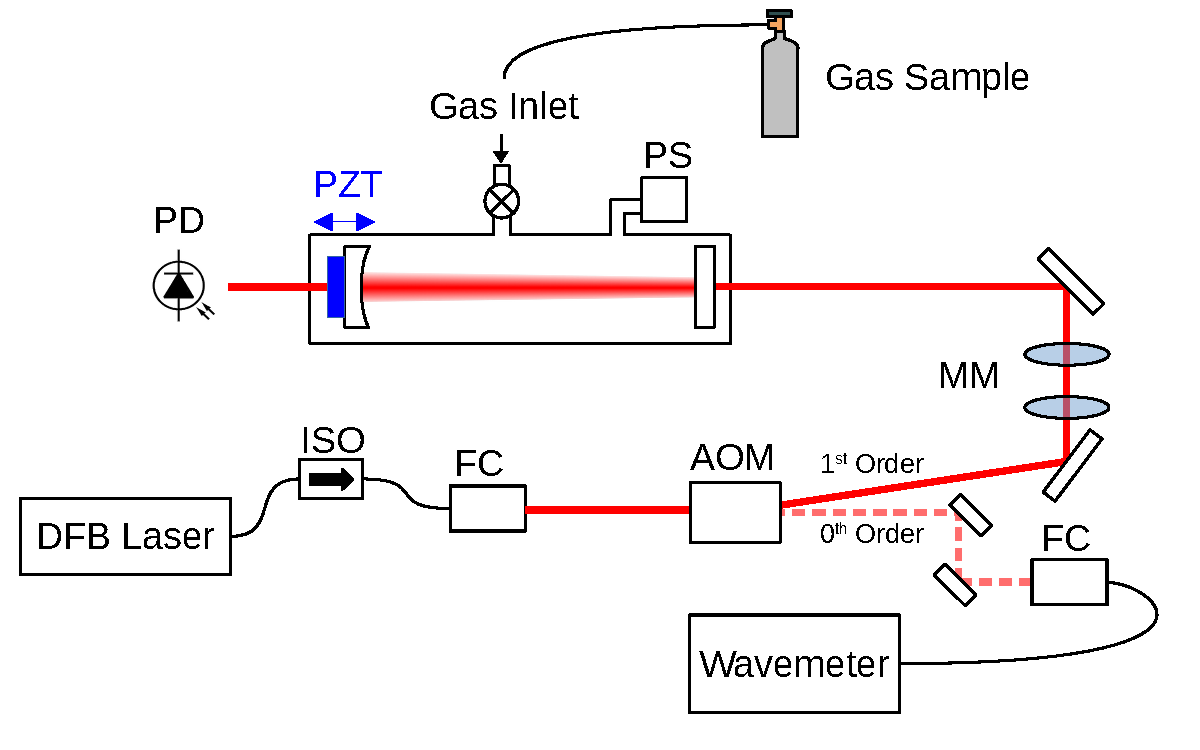
\includegraphics[width=0.85\linewidth]{diagrams/crds_experimentalSetup_noPC}
		\caption{Basic optical configuration for ringdown measurement. The setup includes: distributed feedback (DFB) laser diode, an isolator (ISO), a fiber collimator (FC), an acousto-optic modulator (AOM), switching-off the 1st order deflected beam, a high finesse optical cavity with planar and concave high reflectivity mirrors, a pressure sensor (PS), and a piezoelectric actuator (PZT). The zero order beam emerging from the AOM is coupled with a fiber coupler (FC) into a single mode fiber and sent to the wavemeter.}
		\label{fig:crds_experimentalsetup_nopc}
	\end{figure}
	
	The first-order beam emerging from the AOM is utilized to excite the cavity resonance, as it can be extinguished rapidly by deactivating the RF source. Commercial RF switches are readily available and capable of achieving sub-10ns shut-off times for high-power RF sources. In our setup, we used an RF driver which directly incorporated in the unit a high-speed TTL shutoff signal input. The shutoff time of the first-order beam was measured to be $<$100ns. While this duration could be further reduced by minimizing the beam diameter within the AOM interaction region, the observed value was sufficient to ensure the observation of clean exponential decays.
	
	The challenges associated with maintaining wavelength overlap with a cavity resonance were discussed in Sec. \ref{sec:cav_laser_sweep}, where it was proposed that periodic sweeps of sufficient amplitude could be implemented by exploiting the periodic nature of cavity transmission. To this end, we employ a piezoelectric actuator (PZT), shown in Fig. \ref{fig:crds_experimentalsetup_nopc}, to modulate the cavity length. The PZT is integrated between the cavity mirror and its mechanical mount, providing minute longitudinal displacements under the application of high electric potentials \cite{book_piezoelectric}. Such actuators are ideal for this application as they introduce minimal disruption to the rigid mechanical mounting of the mirrors, owing to their construction from stiff ceramic materials without internal moving parts. Although the displacement range of these devices is limited, an excursion of only $\sim \lambda / 2$ is sufficient to sweep a cavity resonance across a fixed wavelength (see Eq. \ref{cav_resonance_length}). Furthermore, the actuation response of PZT-based systems is remarkably fast--primarily limited by the mass of the attached mirror \cite{book_piezoelectric}--and these devices can also be utilized for active cavity length stabilization to maintain resonance with the laser.
	
	For precise control of the gas mixture measured by the cavity ring-down technique, the optical cavity is constructed inside of a vacuum chamber. The pressure of the chamber is monitored by a pressure sensor (PS). Two separate pressure transducers are used; one is a diaphragm-type pressure gauge (Vacuum Research 902321), providing a measure of the total pressure inside the chamber which is independent of gas composition. The other is a thermocouple gauge (Varian 531) used to verify that a pressure of $<10^{-3}$ Torr is obtained when evacuating the chamber using a fore-pump (Leybold, Scrollvac SC15D).
	
	In order to trigger the AOM shutoff at near the peak of the cavity transmission near a resonance event, a high-speed FPGA-based trigger system is implemented. This system monitors the pre-amplified photodiode signal and gives a low-latency trigger signal to the AOM drive electronics as soon as a rise of sufficient amplitude is detected, allowing for the immediate shutoff of the laser light exciting the cavity. After generating the trigger signal, the FPGA also records the subsequent photodiode signal to a low-latency buffer that is read by the operating system of the host single board computer.
	
	The single board computer which performs this signal acqusition also performs a least squares fit using a model exponential function of the form (\ref{crds_model_exponential}) to the ringdown transient data using a highly optimized routine implementing the Levenberg-Marquandt algorithm. Some of these optimizations of the fitting routine are described in Sec. \ref{sec:subsys_rapidLMfit}, and allow the system to finish the fitting procedure in less time than it takes to acquire the next trace. This is an important benchmark, as acquiring ringdown events at even 100\% duty cycle does not require us to store more than two raw recordings of the transient response at a time for simultaneous fitting and acquisition. An example of such a high-throughput system was shown in Figs. \ref{fig:cavpdhlock} and \ref{fig:cavpdhlockoutput}, where a laser is locked to a cavity resonance and intensity modulated. The resulting filtered cavity output gives the most rapid possible measure of the ringdown time.
	
	Shown in the diagram is a wavemeter which has as its input the fiber-coupled light from the 0th order output of the AOM. This configuration is used to prevent siphoning off any of the laser power using beam splitters or fiber couplers, avoiding any loss of signal to noise ratio. The wavemeter is Michelson interferometer based, and is shown in detail in Fig. \ref{fig:wlwavemetersetup}.
	
	\section{Measurement of the Ringdown Time}
	Discussed in this section are practical considerations for the measurement of cavity ringdown time from the type of shut-off transient discussed in \ref{sec:cav_crds}.
	
	\subsection{Effect of Detector Bandwidth} \label{sec:crds_detBandwidth}
	Detection of the transient decay event requires a photodetector with sufficient bandwidth to provide an undistorted recording of the signal. Further increasing the bandwidth tends to increase noise especially with amplified detectors having gain in the region of high frequency dark noise. There is also diminishing return in increasing the bandwidth much beyond the cavity FSR, as non-exponential transient effects of the cavity output begin to be resolved (see Sec. \ref{sec:cav_crds}). In this section we will establish the lower limit of the detector bandwidth as approximately $1/\tau$.
	
	Here we consider a photodetector which has a high frequency cutoff which behaves as a single-pole low-pass filter \cite{Su_analogFilters}. For photodetectors which incorporate a photodiode with some transimpedance amplifier having some gain $R$, the first order cutoff is generally given by $\omega_d = 1/RC \equiv 1/\tau_d$, where $C$ is the internal capacitance of the photodiode \cite{Horowitz_ArtOfElectronics}. We model this detector by the normalized impulse response
	\begin{equation}
		h(t) = \frac{\theta(t)}{\tau_d}e^{-t/\tau_d}
	\end{equation}
	The step function $\theta(t)$ enforces a causal filter which can only depend on past values of the input. The true decay signal we model by step function build-up with an exponential decay having true ringdown time $\tau$
	\begin{equation}
		s(t) = \theta(t) e^{-t/\tau}
	\end{equation}
	The response of the photodetector is given by the convolution integral
	\begin{align}
		y(t) = (s*h)(t) &= \int_{-\infty}^{\infty}s(t-t')h(t')dt' \\
		&= \frac{1}{\tau_d}\int_{0}^{t}e^{-(t-t')/\tau}e^{-t'/\tau_d}dt' \\
		%&= e^{-t/\tau}\frac{\tau}{\tau_d - \tau}\left[e^{t/\tau}e^{-t/\tau_d} - 1\right] \\
		y(t) &= \frac{\tau}{\tau - \tau_d}\left[e^{-t/\tau} - e^{-t/\tau_d}\right]
	\end{align}
	The observed signal contains a difference of two exponentials with different time constants. If the detector response time $\tau_d$ is much smaller than the true ringdown time, then we have the approximation of the photodetector response holding for $t>\tau_d$
	\begin{equation}
		y(t) \approxeq e^{-t/\tau}
	\end{equation}
	
	When fitting the decay curve, the initial buildup event should be trimmed so that we only fit in the region of the exponential decay. We see from the above single-pole filter example that the data should additionally be trimmed of the transient response of this filter \cite{frontiers_mol_spec}. During the time $t<\tau_d$, we see the buildup is dominated by the detector response time
	\begin{equation}
		y(t) \approxeq 1- e^{-t/\tau_d}
	\end{equation}
	
	Although we only modeled the photodetector bandwidth limitation as a single-pole filter, the result holds in general that the photodetector bandwidth $\Delta f_\mathrm{PD}$ should at least exceed $1/\tau$. We should also expect to trim the recorded decay trace by an amount of time $\sim 1/\Delta f_\mathrm{PD}$ corresponding to the transient response of the detector to prevent the introduction of systematic effects into the measurement of the ringdown time.
	
	\subsection{Statistics of the Ringdown Fits}
	In the experimental determination of the cavity ring-down time, several factors can cause the observed decay rate to deviate from the theoretical value given by Eq. (\ref{crds_tau}) which arises purely from losses due to intra-cavity absorption and the finite mirror reflectivities. Potential sources of such deviations include coupling to higher-order transverse cavity modes \cite{crds_noise_higherOrderModes}, scattering, and mechanical vibrations. Certain error sources introduce non-exponential components into the decay signal, which induce systematic errors if a purely exponential model is employed for the fit. Such features in the cavity output were analyzed numerically and analytically in Sec. \ref{sec:cav_td_response}.
	
	In this analysis, we assume that all sources of non-exponential decay have been minimized and investigate the error arising from fitting a simulated decay curve consisting solely of the signal superimposed with random noise. For the detector employed in this experiment (Thorlabs PDA10CS), the primary noise sources were electronic noise introduced by the preamplifier circuitry and noise induced by electromagnetic interference.
	
	\subsubsection{Simulated Ringdown Data}	
	We simulate the effect of detector technical noise by taking a pure exponential decay signal of unit magnitude and add to it random noise from a normal distribution and a uniform distribution. A fit of the model equation $y(t) = Ae^{-t/\tau} + B$ is made to this simulated detector signal, from which a measure of the ringdown time $\tau$ is extracted.
	
	\begin{figure}[H]
		\centering
		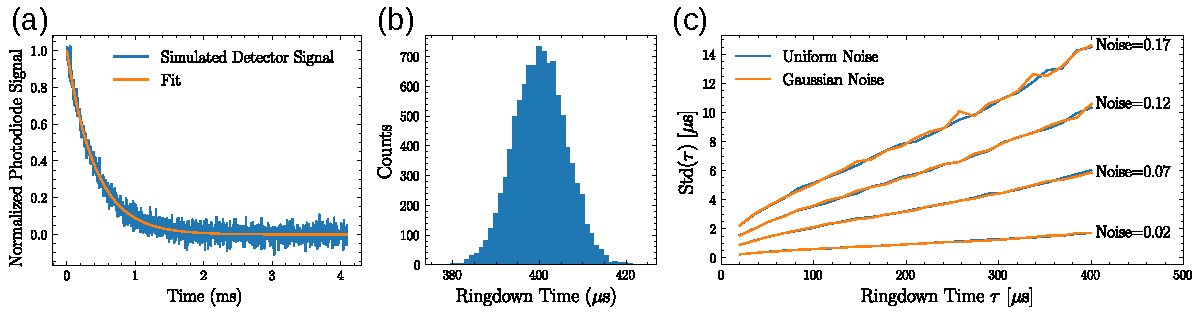
\includegraphics[width=1.0\linewidth]{diagrams/crds_fitNoise}
		\caption{Statistics of fitting ring-down curves with simulated noise. Shown in a) is a ringdown trace with added artificial noise. In b), the histogram of ring-down times obtained from many such fits. The dependence this histogram width (calculated by the standard deviation) is plotted in c) against the true ring-down time, showing a slope dependent on the level of noise.}
		\label{fig:crds_fitNoise}
	\end{figure}
	
	In Fig. \ref{fig:crds_fitNoise}(a), such a simulated signal is displayed alongside a corresponding fit.
	To evaluate the statistical uncertainty, numerous simulated signals are generated for each ring-down time (with $A=1$), varying only the stochastic component of the noise. The histogram in Fig. \ref{fig:crds_fitNoise}(b) represents the distribution of simulated ring-down measurements for a true value of $\tau = 400\,\mu\text{s}$, subject to normally distributed noise with a standard deviation of $0.07$ relative to the unit signal (A=1). By varying the true ring-down time and calculating the resulting deviation of these measurements, we obtain the plots shown in Fig. \ref{fig:crds_fitNoise}(c). It is observed that the standard deviations of the measurements, defined as $\Delta \tau$, are proportional to the true ring-down time $\tau$. Given that the mean of the measurements $\bar{\tau}$ converges to this true value, we observe that for a sufficiently large sample, the ratio of the standard deviation to the mean remains a constant characteristic of the system's technical noise
	\begin{equation} \label{crds_tau_std}
		\frac{\Delta \tau}{\bar{\tau}} = \text{const}
	\end{equation}
	The invariance of this ratio -- the relative uncertainty -- indicates that ring-down time measurements limited by technical noise follow a log-normal distribution.
	
	The precision of the absorption coefficient determination via equation (\ref{crds_alpha}) is fundamentally limited by the precision of the ring-down time measurement. If the ring-down time is known with an uncertainty $\Delta \tau$, the resulting uncertainty in the absorption coefficient (assuming a perfectly known $\tau_0$) is given by
	\begin{equation} \label{crds_alpha_err}
		\Delta \alpha = \frac{\Delta \tau}{\bar{\tau}} \frac{1}{c\bar{\tau}} 
	\end{equation}
	Since the ratio $\Delta \tau / \bar{\tau}$ is a constant characteristic of the system's technical noise, the absorption sensitivity improves as the baseline ring-down time increases. This suggests that a longer cavity should yield improved sensitivity for a given set of mirrors; however, it must be noted that the ratio $\Delta \tau / \bar{\tau}$ is also expected to increase in longer cavities due to the increased susceptibility to mechanical jitter.
	
	\subsection{Experimental Data and the Precision of the Ringdown Time}
	The precision with which absorption at a single wavelength can be measured using CRDS is fundamentally limited by the uncertainty in the ringdown time quantification, as established by equation (\ref{crds_alpha_err}). The precision of the ring-down time estimate can be improved through temporal averaging. Specifically averaging $N$ independent measurements yields a standard deviation that scales as $\propto \Delta \tau / \sqrt{N}$, where $\Delta \tau$ represents the standard deviation of individual measurements. While this scaling holds for measurements following a perfect log-normal distribution, real-world experimental conditions impose a limit on the reduction of variance via averaging. This limitation is primarily attributed to drifts in the true ringdown time over longer integration periods.
	
	The Allan variance and the modified Allan variance \cite{allan_variance_mod} are computational procedures used to determine, from a sequence of ringdown measurements, both the optimal averaging time and the minimum achievable uncertainty $\Delta \tau$ through integration. This analysis enables the determination of the minimum detectable absorption. Equivalently, the Allan variance can be calculated directly from measurements of the absorption coefficient to yield the fundamental limit on the variance of $\alpha$.
	
	Both procedures process a sequence of measurements $\tau_{1\ldots N}$ by partitioning them into $m$ groups of size $p$, constructing an averaged measurement $A_n(p)$, where $n$ denotes the $n^\mathrm{th}$ average in the sequence. Fig. \ref{fig:crds_allan_diagram} illustrates the construction of these averaged sequences for both methods. Denoting $A'_n(p)$ as the sequence generated by the modified algorithm, the averages are defined as
	\begin{align}
		A_n(p) &= \frac{1}{p} \sum_{i=1 + p(n-1)}^{np}\tau_i& n=1\ldots m && m = \mathrm{floor}(N/p)  \\
		A'_n(p) &= \frac{1}{p} \sum_{i=n}^{p+n-1}\tau_i& n=1\ldots m && m = N - p + 1
	\end{align}
%	\begin{align}
%		A_n(p) &= \frac{1}{p} \sum_{i=1 + p(n-1)}^{np}\tau_i, & n=1\ldots m, && m = \lfloor N/p \rfloor \\
%		A'_n(p) &= \frac{1}{p} \sum_{i=n}^{p+n-1}\tau_i, & n=1\ldots m, && m = N - p + 1
%	\end{align}
	While the modified algorithm generates a significantly larger number of averages, these values are highly correlated, as demonstrated in Fig. \ref{fig:crds_allan_diagram}. Additionally, the modified algorithm utilizes all of the data, which is in contrast to the standard algorithm where the last $N - mp$ samples are discarded, a value that fluctuates as the value of $p$ is changed.
	
	\begin{figure}[H]
		\centering
		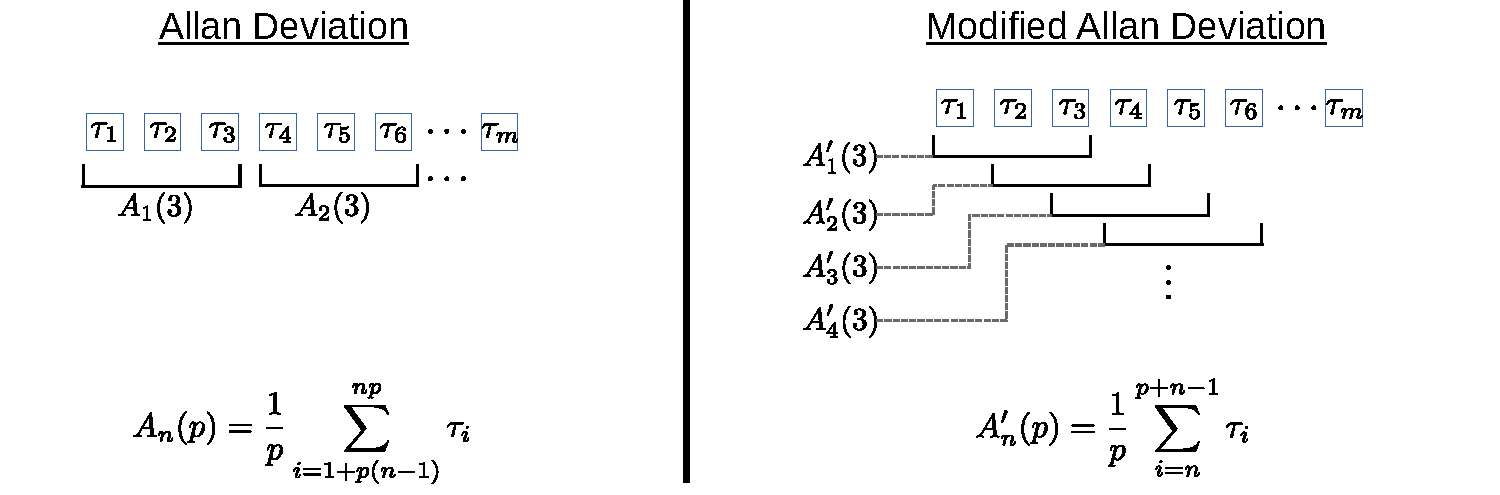
\includegraphics[width=0.9\linewidth]{diagrams/crds_allanDiagram}
		\caption{Construction of the sequence of averages used for the computation of the standard Allan deviation and the modified Allan deviation for an averaging length of $p=3$. In both cases, a sequence of measurements is taken as input to compute sequence of averaged measurements ($A_n(p)$ and $A'_n(p)$).}
		\label{fig:crds_allan_diagram}
	\end{figure}
	
	For a given averaging size $p$, a single sample of the Allan variance is constructed from successive pairs of $A_n(p)$ for the standard algorithm, while the modified Allan variance is constructed from successive pairs of $A'_n(p)$. The $n^\mathrm{th}$ samples of the standard Allan variance $\sigma^2_{A,n}(p)$ and the modified Allan variance $\sigma^2_{A',n}(p)$, both corresponding to an averaging size $p$, are defined as
	\begin{align}
		\sigma^2_{A,n}(p) &= \frac{1}{2}\Big[A_n(p) - A_{n+1}(p)\Big]^2 \\
		\sigma^2_{A',n}(p) &= \frac{1}{2}\Big[A'_n(p) - A'_{n+p}(p)\Big]^2
	\end{align}
	In the standard algorithm, successive pairs of averages are uncorrelated; however, in the modified algorithm, there is a strong correlation between successive samples of the variance, $\sigma^2_{A', n}$ and $\sigma^2_{A', n+1}$.
	
	The time-averaged Allan variance, computed over the $m$ constructed averages for a chosen value of $p$, is given by
	\begin{equation}.
		\Bigl \langle \sigma_A^2(p) \Bigr \rangle_t = \frac{1}{2(m-1)}\sum_{n=1}^{m-1}\Big[A_i(p) - A_{i+1}(p)\Big]^2
	\end{equation}
	Similarly, the time-averaged modified Allan variance is expressed as
	\begin{equation}
		\Bigl \langle \sigma_{A'}^2(p) \Bigr \rangle_t = \frac{1}{2(N+1-2p)}\sum_{n=1}^{N-2p}\Big[A'_n(p) - A'_{n+p}(p)\Big]^2
	\end{equation}
	
	Fig. \ref{fig:crds_detectionlimit} presents a histogram of many consecutive ringdown time measurements. Under the assumption of a normal distribution, increasing the number of averaged measurements $p$ should theoretically allow the precision of the mean estimate to improve monotonically as $1/\sqrt{p}$. The Allan deviation plot in Fig. \ref{fig:crds_detectionlimit} identifies the integration time at which this improvement begins to degrade. In the initial portion of the plot, the traces exhibit a downward trend; on these log-log axes, this appears as a straight line with a slope of $-1/2$, confirming that the ringdown time estimate improves as $1/\sqrt{p}$ during the early stages of averaging. However, this trend does not continue indefinitely, as the Allan plot eventually reaches a minimum, marking the onset of non-stationary noise or drift.
	
	The minimum of the Allan plot represents the minimum achievable variance for the ringdown time measurement, and therefore defines the fundamental detection limit of the system. The position of this minimum identifies $p_\mathrm{opt}$, the optimal number of averages. In practice, Allan plots are frequently presented as a function of integration time rather than the number of averages; this is physically motivated, as drift-induced errors typically manifest over specific timescales. In regimes where such drift errors dominate, increasing the sampling rate of the ringdown measurements $\tau_i$ will generally result in an increased $p_\mathrm{opt}$ and a lower detection limit. Consequently, when comparing different experimental setups with disparate acquisition rates, the intrinsic stability of a system is most effectively characterized by its optimum integration time.
	
	\begin{figure}[H]
		\centering
		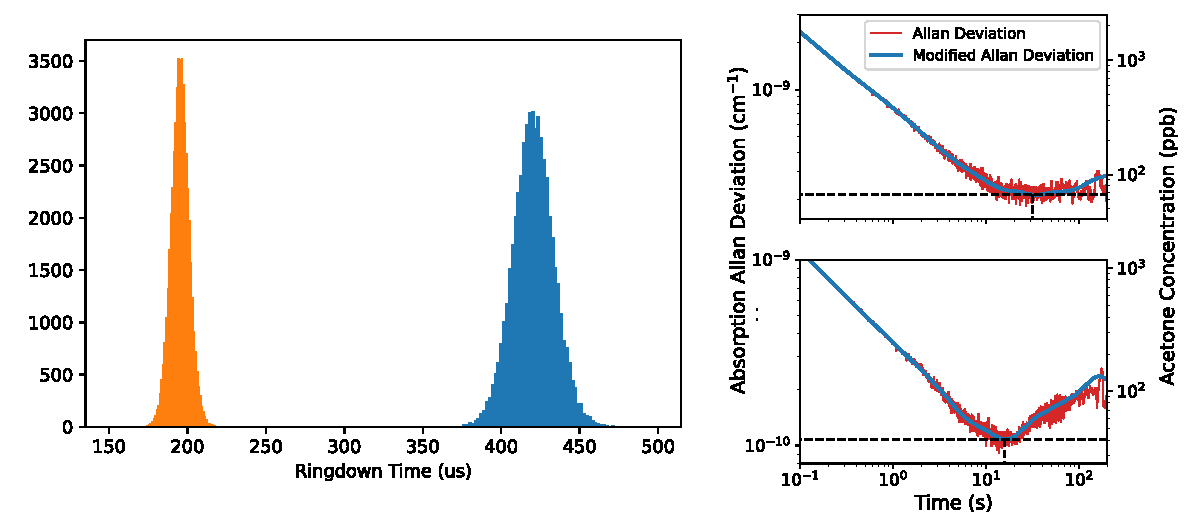
\includegraphics[width=0.85\linewidth]{diagrams/crds_detection_limit}
		\caption{Histograms showing two different measurements of ringdown time at two different wavelengths. The dependence of the variance on the mean ringdown time value is clear in the histogram. On the right, Allan deviations are computed which give measurements of the detection limit. The upper allan plot corresponds to the lower ringdown time measurement and the lower plot corresponds to the greater ringdown time measurement.}
		\label{fig:crds_detectionlimit}
	\end{figure}
	
	\subsection{Multi-Wavelength Detection Limit}
	For a single ring-down measurement, the detection limit is defined as the absorption which produces a change in ring-down time equal to the standard deviation of the baseline ring-down time $\Delta \tau$. The ultimate obtainable value for $\Delta \tau$ after averaging is assessed through the Allan deviation.  This gives the detection limit of a single ring-down measurement as (\ref{crds_alpha_err}), which can be converted to a number density uncertainty
	\begin{equation}
		\Delta n = \frac{1}{\sigma(\lambda)}\frac{\Delta \tau}{\bar{\tau}} \frac{1}{c\bar{\tau}}
	\end{equation}
	It is clear that the uncertainty in the actual concentration of a particular gas species depends on the magnitude of $\sigma(\lambda)$. For a strongly absorbing species, we can report a lower detection limit than for a weakly absorbing species.
	
	For a laser which scans across many wavelengths, a different approach must be taken to account for the spectral structure and the variation of $\Delta \tau$ over this range. If we use the fact that the ratio $\Delta \tau / \bar{\tau}$ is constant for CRDS systems limited by technical noise, then we may make use of (\ref{error_conc_alpha}) to evaluate the detection limit for several species measured simultaneously with a spectral scan. This gives for the detection limit of the $i^\mathrm{th}$ species 
	\begin{equation}
		\Delta c_i = \sqrt{\sum_j M_{ij} \Delta \alpha_j} = \frac{\epsilon}{c} \sqrt{\sum_j M_{ij} / \bar{\tau}_j}
	\end{equation}
	In the above relation, $M = (A^TA)^{-1} A^T$, where $A$ is the non-square matrix constructed from the over determined system (\ref{fit_spectrum}), and $\epsilon = \Delta \tau / \bar{\tau}$ is the constant ratio describing the performance of the CRDS system. For each $j^\mathrm{th}$ spectrum point, the mean ringdown time $\bar{\tau}_j$ is used in the evaluation of the above detection limits.
	
	\section{Acquisition System}
	The acquisition system consists of a single
	board computer (Red Pitaya STEMlab 125-14, Solkan, Slovenia) which has onboard 14-bit
	analog-to-digital converter (ADC) and a field-programmable gate array (FPGA), which
	is used to provide a low-latency switching signal to the AOM driver, allowing the laser
	to shutoff when resonant excitation of the cavity is detected on the photodiode (PD) by a
	rapid signal rise to a pre-defined threshold. This single board computer also performs the
	fitting of the exponentially decaying signal of the transmitted through the cavity light with
	the model Equation (\ref{crds_model_exponential}). The amplitude term A captures variations in the coupling between the laser and cavity.
	
	The analog ring-down signal is processed using a low-noise pre-amplifier (Stanford
	Research Systems SR560, Sunnyvale, CA , USA) which features a 1 MHz single-pole low-pass filter. This signal is acquired at 125 MHz sampling rate by the acquisition system, which
	is down-sampled to 125/64 MHz. Additional digital filtering is performed by the FPGA
	prior to down-sampling in order to reduce noise aliased to low frequency \cite{frontiers_mol_spec}. The down-sampled signal is stored in the RAM of the single-board computer and passed to the
	operating system, which is then fit using an optimized fitting routine written in C. The initial
	portion of the recording is trimmed to remove the cavity buildup and corresponding
	transients \cite{frontiers_mol_spec}.
	
	The signal is recorded using 4000 data points and the fit is conducted with 20 iterations
	of the Levenberg–Marquardt algorithm. This fitting is performed on the same single board
	computer which performs the measurement to avoid additional latency from transferring
	the analog trace. An initial guess of the parameters is calculated using the Fourier transform
	method of \cite{fourier_transform_exponentialDecay} using the FPGA of the acquisition system to perform the Fourier integrals
	in real time.
	
	\section{Laser Source and Tuning}
	For CRDS, we a commercially available distributed feedback diode laser (DFB) available as a 14-pin butterfly package. These packages typically contain onboard thermoelectric coolers and a temperature sensor usually in the form of a standard 10k$\mathrm{\Omega}$ thermistor. The package is attached to a commercially available heatsink which features convenient D-SUB connectors for connection to a laser diode controller.
	
	\begin{table}[H]
		\begin{center}
			\caption{DFB laser diodes used for NIR measurements of cavity ring-down time. Details of the tuning profile measurements are discussed in Ch. \ref{chap:det}. The model numbers for the lasers are additionally given in Table. \ref{table:diodes}.} \label{table:crds_diodes}
			\begin{tabular}{|c|c|c|c|c|c|c|c|}
				\hline
				No. & Manufacturer & Lower & Upper  & Meas. Tuning & Meas. Tuning \\
				& & Range & Range & (nm/mA) & (nm/$^\circ$C) \\
				\hline
				1 & Eblana & 1651.4 nm & 1655.2 nm & 2.04$\times10^{-2}$ & 9.95$\times10^{-2}$ \\
				\hline
				2 & Eblana & 1657.7 nm & 1662.0 nm & 2.57$\times10^{-2}$ & 1.12$\times10^{-1}$ \\
				\hline
				3 & Eblana & 1671.6 nm & 1675.6 nm & 2.03$\times10^{-2}$ & 1.05$\times10^{-1}$ \\
				%\hline
				%4 & NEL & - & - & - & - & -\\
				\hline
			\end{tabular}
		\end{center}
	\end{table}
	
	The laser wavelength is tuned by changing the temperature and injection current of the
	laser diode, both of which are controlled by GPIB communication between the computer
	and the laser diode controller. Fine control of the laser wavelength is
	established by adjusting the laser diode injection current. The laser current is stabilized
	within 25 ppm with a resolution of 0.01 mA using a Newport LCM-39420 module in an
	LDC-3900 laser diode controller. For course wavelength adjustment, the temperature of the
	diode is actively stabilized by the LCM-39420 module. The set point of this stabilization can be adjusted to a precision of 0.1$^\circ$C.
	
%	\begin{figure}[H]
%		\centering
%		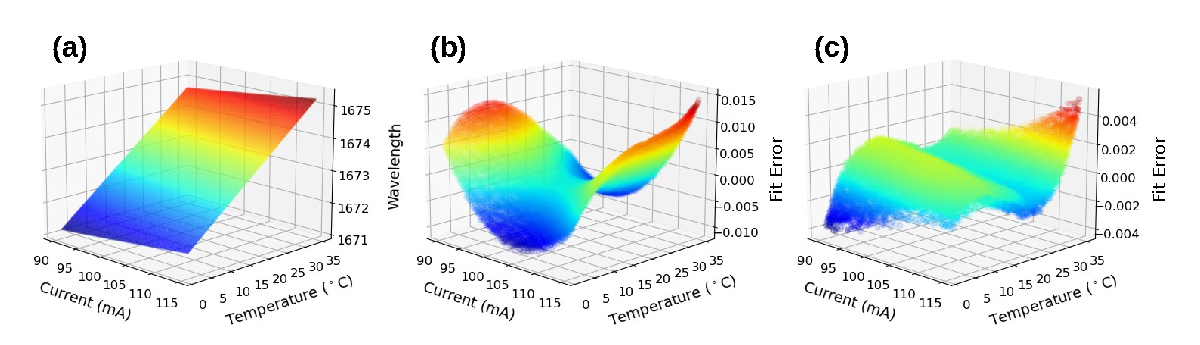
\includegraphics[width=1.0\linewidth]{diagrams/crds_detuningSurface}
%		\caption{Plot of wavelength against the temperature and injection current of a DFB laser diode (number 3 in Table \ref{table:crds_diodes}). Shown in (a) are $\sim$34,000 measured wavelength values as the temperature and current are scanned. In (b) a plane fit is subtracted from the data showing systematic deviation from this planar behavior. A paraboloid fit is subtracted from the data in (c) in which we see only small deviations from this fit. \textbf{ALL Z-AXES NEED [nm] UNITS!}}
%		\label{fig:crds_detuningsurface}
%	\end{figure}
	
	
	The scan of the laser wavelength is conducted by first scanning the laser current from 110.00 to 109.00 mA. After finishing the scan of laser current, the temperature is changed by 0.2$^\circ$C and the current scan is reset. This scan order is preferred to minimize the frequency of temperature changes of the laser diode since there is a longer time required for the laser to settle into a stable wavelength with temperature variations compared to changes in the current. The tuning behavior of the laser diodes used in this work are explored in detail in Ch. \ref{chap:det}, and plotted in Fig. \ref{fig:det_detuningsurface}.
	
	\subsection{Characterizing the Speed of Laser Temperature Tuning} \label{sec:crds_tuning_speed}
	As discussed in the preceding section, the temperature of the laser diode can serve as a coarse tuning mechanism for the wavelength by adjusting the set-point of the temperature controller's stabilization loop. In this section, we characterize the temporal dynamics and the rate at which such tuning can be performed.
	
	We use the dynamic wavelength retrieval (DWR) method presented in Sec. \ref{sec:wl_tracking} to characterize the temporal dependence of the laser wavelength following discrete step changes in the temperature controller set-point. This approach also serves to verify the mode-hop-free tuning range of the laser.
	
	\begin{figure}[H]
		\centering
		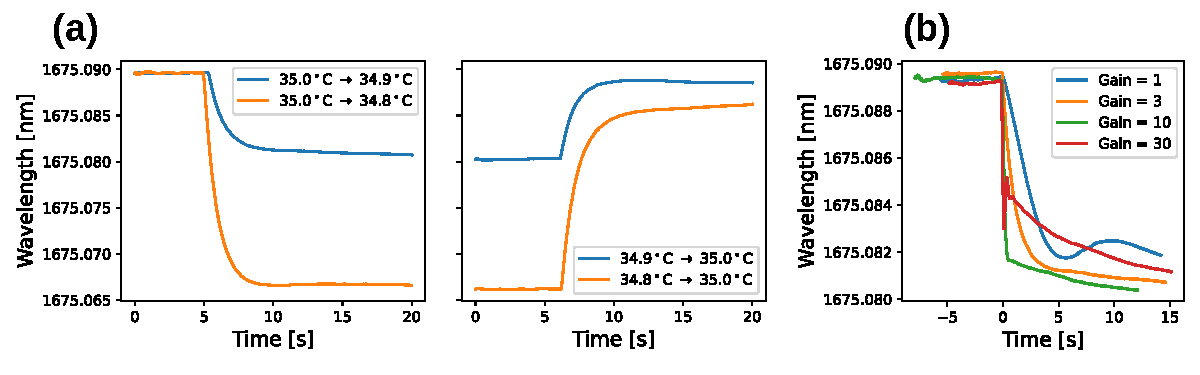
\includegraphics[width=1.0\linewidth]{diagrams/crds_diode_temperatureTuning}
		\caption{Temporal dependence of the DFB laser diode tuning, measured using the Dynamic Wavelength Retrieval (DWR) method described in Sec. \ref{sec:wl_tracking}. In (a), the laser wavelength is tracked following temperature step functions directed both toward and away from a common target value, illustrating the presence of thermal hysteresis. In (b), we investigate the impact of varying loop gains within the temperature control feedback loop. A gain of 3 was selected as an optimal compromise between tuning speed, overshoot, and residual drift.}
		\label{fig:crds_diodeTuningSpeed}
	\end{figure}
	
	Based on these observations, a waiting time of approximately 10 seconds was determined to be necessary for sufficient laser equilibration. However, as illustrated in Fig. \ref{fig:crds_diodeTuningSpeed}, the wavelength may still exhibit slow drift even after this period has elapsed. If the CRDS system acquisition rate is sufficiently high, this drift will have a minimal effect on the averaged measurements.
	
	\section{Fitting the Ringdown Spectrum}
	In this section, we motivate the use of (\ref{leastSquares}) to find the concentration of gas species from a spectrum measured using CRDS through the non-interacting gas approximation. We arrive at a weight function which accounts for the statistics of ringdown time measurements conducted under conditions of technical noise limitations.
	
	The measured spectrum consists of the averaged ringdown times recorded as a function of the laser wavelength driving the cavity resonance. To determine the absorption coefficient, equation (\ref{crds_alpha}) is used to convert these measured ring-down times into absorption values. This calculation requires the baseline ringdown time, $\tau_0$, which is measured by evacuating the chamber to eliminate all absorbing species. As expressed in equation (\ref{crds_tau_vac}), $\tau_0(\lambda)$ depends on the mirror reflectivity $R(\lambda)$, which may exhibit wavelength dependence. To account for this, we measure the baseline ringdown time across the entire tuning range. Under optimized cavity alignment, the baseline was found to be well-described by a linear relationship. A linear fit was therefore used to interpolate the wavelength-dependent $\tau_0(\lambda)$ required for equation (\ref{crds_alpha}).
	
	Cavity ringdown spectroscopy is particularly well-suited for measuring trace concentrations of gaseous species. Consequently, it is appropriate to operate within the non-interacting gas approximation discussed in Sec. \ref{sec:non_interacting_gas}. In this regime, equation (\ref{leastSquares}) can be used to retrieve individual species concentrations, provided their absorption cross-sections are well-characterized across the scanned wavelength range. However, as previously demonstrated in \cite{mine_acetone}, the accuracy of this retrieval can be enhanced by implementing a weighting function that accounts for the ordinate dependent uncertainty in the measured ringdown times, as characterized by equation (\ref{crds_tau_std}).
	
	%Cavity ringdown spectroscopy is particularly suited for the measurement of small concentration gas species. For this reason, it is reasonable to operate in the non-interacting gas approximation discussed in Sec. \ref{sec:non_interacting_gas}. In this regime, we may use equation (\ref{leastSquares}) to retrieve the concentrations of the individual species given that their cross sections are well-known in the wavelength range of the scan. However, it was pointed out in our paper \cite{mine_acetone} that this can be improved using a weight function which accounts for the changing deviation of the measured ringdown times characterized by (\ref{crds_tau_std}). 
	
	For ringdown time measurements dominated by technical noise rather than systematic effects, the relative uncertainty $\Delta\tau/\bar{\tau}$ remains approximately constant \cite{vanZee_1999}, where $\bar{\tau}$ denotes the mean of the measurements. This behavior is confirmed in our experimental results, as illustrated by the histograms in Fig. \ref{fig:crds_detectionlimit}.
	
	When transforming measurements via a function $f(\tau)$, the uncertainty in the resulting values is given by $\Delta f \approx |f'(\bar{\tau})| \Delta \tau$. By choosing $f(\tau) = \ln(\tau/\tau_0)$, the uncertainty becomes $\Delta f = \Delta \tau/\bar{\tau}$, which is approximately constant. This implies that error minimization should be performed in the space of \textit{logarithmic} ring-down times. The model absorption from the non-interacting gas approximation (\ref{alpha_dilute}), denoted as $\alpha_\mathrm{m}(\lambda)$, can be converted into a model instrument response using the inverse of equation (\ref{crds_alpha})
	\begin{equation}
		\tau_\mathrm{m}(\lambda) = \frac{1}{c\alpha_\mathrm{m}(\lambda) + 1/\tau_0}
	\end{equation}
	Defining $\tau_i$ as the $i$-th measured ringdown time, the error in the logarithmic ringdown time is expressed as
	\begin{align} %\label{error_log}
		\mathrm{E}_\mathrm{L} &= \sum_i \Big[\ln \frac{\tau_i}{\tau_0} - \ln\frac{\tau_\mathrm{m}(\lambda_i)}{\tau_0}\Big]^2 \nonumber \\
		&= \sum_i \Big[\ln \frac{\tau_i}{\tau_0} + \ln\big(1+c\tau_0\alpha_\mathrm{m}(\lambda_i)\big)\Big]^2
	\end{align}
		
	The weighted fit procedure discussed in Sec. \ref{sec:weighted_fit} can be used to correct for a transformation of the ordinate values. There we give the general formula (\ref{weight_function}) for a weight function which corrects the linear least squares formula for minimizing the error in the space of the instrument response. The linear least squares procedure is most effective when the ordinate values have similar variance. We define the homoscedastic quantity
	\begin{equation}
		q \equiv \ln \left(\frac{\tau}{\tau_0}\right)
	\end{equation}
	The inverse of this expression $\tau = \tau_0 e^q$ which is inserted into formula (\ref{crds_alpha}) for the absorption coefficient in terms of the $q$ quantity
	\begin{equation}
		F(q) \equiv \alpha(\tau(q)) = \frac{1}{c\tau_0}\left(e^{-q} - 1\right)
	\end{equation}
	We also require the derivative of this function evaluated at $q = q_0 = 0$
	\begin{equation}
		F'(q_0) = \frac{-1}{c\tau_0}e^{-q_0} = \frac{-1}{c\tau_0}
	\end{equation}
	From formula (\ref{weight_function}), the weight function corresponding to the minimization of error in logarithmic ringdown times is
	\begin{equation}
		w(q) = F'(q_0)\frac{q - q_0}{F(q)} = -\frac{q}{e^{-q} - 1}
	\end{equation}
	We write this now in terms of just the ringdown time $\tau$ and the baseline ringdown time $\tau_0$
	\begin{equation}
		w(\tau) = \tau \frac{\ln\left(\tau/\tau_0\right)}{\tau - \tau_0}
	\end{equation}
	This is precisely the weight function that was derived in \cite{mine_acetone} by comparing terms of the series expansions for the different error measures. This derivation is summarized in \ref{sec:append_weight_series_crds}. This weight function allows us to approximate the solution to the nonlinear fitting problem of minimizing $\mathrm{E}_\mathrm{L}$ by using the weighted linear least squares formula in equation (\ref{fit_spectrum_weighted}).
	
	\subsection{Simulation of Weighted Fitting Procedure for CRDS Spectra} \label{sec:simulation}
	We perform Monte-Carlo simulation of the effect of ring-down time measurement noise on the fitting process and compare the effect of using different weighting functions on simulated breath samples. From the simulations, we are able to estimate uncertainty in the concentrations of all gas species measured in this investigation as well as quantify the effect of using different weighting functions and artificial baselines.
	
	We simulated a breath spectrum similar to Fig. \ref{fig:acetone_crds_breathplusacetone} containing 1ppm acetone at 70 Torr. Using parameters in the HITRAN database \cite{hitran_2020} and the concentrations $y_i$ shown in the right-most column of Table \ref{tbl:simulation_errs}, we simulated the absorption cross section of all components reported in Fig. \ref{fig:acetone_crds_breathplusacetone} and summed them to give a simulated breath spectrum $\alpha(\lambda) = \frac{P}{k_B T}\sum_{i}y_i\sigma_i(\lambda)$. We added to this spectrum the expected absorption of 1 ppm acetone using the model reported in this paper.
	
	We converted the simulated breath spectrum into a curve of $\tau(\lambda)$ using a typical fit of the baseline ring-down time $\tau_0(\lambda)$ and added Gaussian noise. At each simulated wavelength $\lambda_i$ the deviation $\Delta \tau$ of this Gaussian noise was chosen to be proportional to $\tau(\lambda_i)$, which is typical of ring-down measurements limited by statistical noise \cite{vanZee_1999}. To model the performance of our spectrometer, the value of $\Delta \tau / \tau$ was chosen to be 0.003, which is typical of a measurement of our setup having 100 averages. This number of averages is well within the linear portion of the dependence shown in the right of Fig. \ref{fig:crds_detectionlimit} and corresponds to a $\Delta \tau$ which is decreasing as the square root of the number of averages.
	
	To each of these simulated noisy ring-down measurements $\tau_i$ we converted them to absorption using $\alpha_i = (\tau_i^{-1}-\tau_0^{-1}(\lambda_i))/c$ and with Eqn. \ref{leastSquares_weighted} found the set of concentrations $y_i$ which give the weighted least squares fit of the simulated breath spectrum. We evaluated the four weighting functions
	\begin{equation*}
		w_\mathrm{u}(\tau) = 1 \qquad
		w_\tau(\tau) = \frac{\tau}{\tau_0} \qquad
		w_\mathrm{L}(\tau) = \frac{\tau\ln\frac{\tau}{\tau_0}}{\tau-\tau_0} \qquad
		w_\mathrm{2L}(\tau) = \frac{w_\mathrm{L}(2\tau)}{w_\mathrm{L}(2\tau_0)}
	\end{equation*}
	on the performance of the recovered concentrations as well as monitored the root-mean-square deviations $\sqrt{\mathrm{E}_{\alpha}}$, $\sqrt{\mathrm{E}_{\tau}}$, $\sqrt{\mathrm{E}_{\mathrm{L}}}$, and $\sqrt{\mathrm{E}_{\mathrm{2L}}}$.
	
	We additionally tested the performance of different models of the absorption baseline. For the fitting model we used the model absorption directly with the offset term
	\begin{equation}\label{alpha_D}
		\alpha_\mathrm{D}(\lambda) = a_0 \sigma_\mathrm{ac}(\lambda) + \sum_{i} a_i \sigma_i (\lambda ;\, T, P)
	\end{equation}
	and compared this to the modified absorption model
	\begin{equation}\label{alpha_B}
		\alpha_B(\lambda) = a_0 \tilde{\sigma}_\mathrm{ac}(\lambda) + \sum_{n=0}^B b_n (\lambda-\lambda_0)^n + \sum_{i} a_i \sigma_i (\lambda;\, T, P)
	\end{equation}
	where $\tilde{\sigma}_\mathrm{ac}$ is normalized peak function from equation (\ref{sigma_tilde}). This modification allows us to determine the acetone cross section independently of baseline errors, essentially only using the shape of the broadband peak for concentration determination. The sum over $n$ is a function used to model the baseline and is a polynomial of order $B$. The term $\lambda_0$ is a term used to center the terms in the range of the scan and we used a value of $\lambda_0=1673.5$ nm for both simulation and data analysis in this work. The sum over $i$ is over the different molecular cross-sections modeled using the HITRAN database at a temperature of $T=296$ K and $P=70$ Torr.
	
	The coefficients $a_{0,i}$ give the gas component concentrations from (\ref{ai}) and the $b_n$ coefficients define the polynomial baseline. Both sets of coefficients are determined using (\ref{leastSquares_weighted}) and we compare the different weighting functions $w_u(\tau)$, $w_\tau(\tau)$, and $w_\mathrm{L}(\tau)$. The choice of $\lambda_0$ affects the $b_i$ coefficients, but gives the same resulting polynomial when expanded for a particular simulated spectrum. However, the numerical stability of the routine used to evaluate (\ref{leastSquares_weighted}) can be improved by choosing $\lambda_0$ in the center of the scan and normalizing the small cross section values for each species.
	
	The results are shown in Fig. \ref{fig:simulationresults} and Tables \ref{tbl:simulation_errs} and \ref{tbl:simulation_errs_acetone}. The use of different baseline polynomial orders $B$ did not significantly affect the determination of the concentrations of the different gas species calculated from the HITRAN database since these correspond to narrow spectrum features. However, since acetone concentration is determined from a broadband feature, the accuracy of concentration determination was generally degraded with increasing $B$.
	
	The model $\alpha_D(\lambda)$ gave the best results when the offset of the absorption feature can be definitively determined as seen in Figure \ref{fig:simulationresults}a. The results of adding a constant offset of $2\times 10^{-9}$ cm$^{-1}$ to the simulated absorption spectra can be seen in Figure \ref{fig:simulationresults}b, where the $\alpha_\mathrm{D}(\lambda)$ model is severely displaced from the expected mean of 1 ppm acetone concentration. The $\alpha_B(\lambda)$ models showed complete immunity to this shift at the expense of higher deviations in the concentration estimate. Although the increased deviations of the $\alpha_B(\lambda)$ models became worse as the baseline polynomial order $B$ is increased, they are increasingly immune to distortions of the baseline.
	
	Shown in Tables \ref{tbl:simulation_errs} and \ref{tbl:simulation_errs_acetone} are the relative errors in the concentrations of various gas species resulting from the fitting process for simulated experimental conditions. The values shown in the table are in agreement with the experimental data repeatability. The choice of weighting function used to fit the simulated spectra did not significantly affect the results for simulated experimental conditions, except for the most common isotopologue of water (see Fig. \ref{fig:simulationresults}c) and acetone (see Fig. \ref{fig:simulationresults}d). Since the absorption peaks of water encompass the largest dynamic range of the measurement, the effect of the weighting function is largest on this species.
	
	To further investigate the effect of the weighting functions on the recovered concentrations, we additionally simulated 100,000 spectra which had a much larger relative noise of $\Delta \tau /\tau = 5\%$. Under the condition of increased noise, the choice of weighting function had a larger effect which can be seen in the results of Table \ref{tbl:simulation_weight_results}. The unweighted fitting procedure tended to slightly overestimate the gas concentrations, while the weighting function $w_\tau$ tended to slightly underestimate concentrations. The weighting functions $w_\mathrm{L}$ and $w_\mathrm{L2}$ gave the best agreement to the exact values and produced the only results which agreed to the exact values one standard error. 
	
	We conclude from these simulations that the best performance is offered by the weighting functions $w_\mathrm{L}$ and $w_\mathrm{L2}$ given by Eq. (\ref{weight_log}) and (\ref{weight_L2}). The direct fitting model $\alpha_\mathrm{D}$ given by Eq. (\ref{alpha_D}) gave the best performance in terms of acetone concentration estimation. However, in the case where the absorption baseline cannot be determined or has some distortion, the best results are then offered by the $\alpha_B(\lambda)$ model given by Eq. (\ref{alpha_B}) with $B$ chosen to capture the effect of the distortion.
	
	\begin{figure}[H]
		\centering
		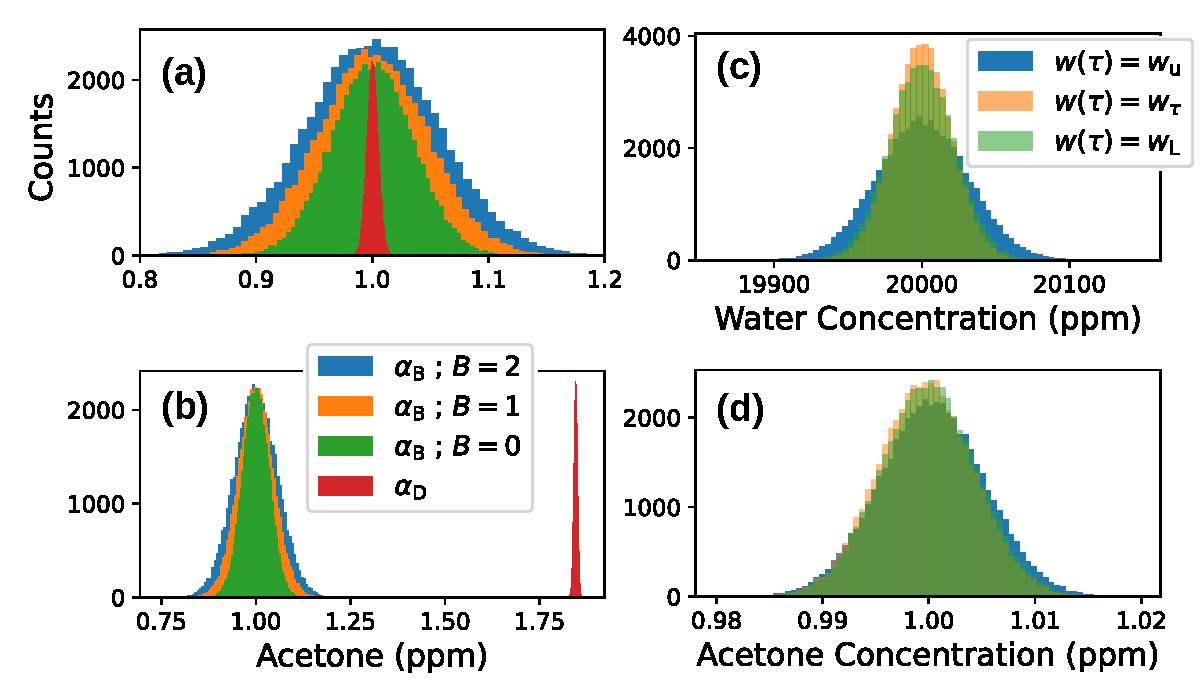
\includegraphics[width=1.0\linewidth]{diagrams/simulationResults}
		\caption{Simulation results showing histograms of recovered concentrations from a simulated breath spectrum spectrum having 1,000 points evenly spaced in the range 1671.5-1675 nm superimposed with Gaussian noise characterized by $\Delta \tau/\tau=0.3\%$. Shown in (a) and (b) is the effect of changing the absorption model. It can be seen in (a) that the best acetone concentration estimate is obtained using the direct model $\alpha_D(\lambda)$, but suffers from sensitivity to baseline offset. Seen in (b) are the results where a constant $2\times10^{-9}$ cm$^{-1}$ absorption was added to the simulated spectra, causing a severe shift of the mean acetone concentration recovered by the $\alpha_\mathrm{D}$ model. Shown in (c) and (d) is the effect of the weighting function $w(\tau)$. The improvement to the water concentration estimate when using the weighting function is shown in (c). A slightly improved acetone concentration estimate is also obtained when using the weight function, as seen in (d).}
		\label{fig:simulationresults}
	\end{figure}
	
	\begin{table}[H]
		\caption{Relative error calculated for each gas concentration $y_i$ as the ratio of the standard deviation to the mean for a set of simulated breath sample measurements having noise characterized by $\Delta \tau/\tau = 0.3\%$. These results are the essentially the same for the different weighting functions with the exception of H$_2$O and acetone, which are shown with $w(\tau)=\tau/\tau_0$. The results are also nearly identical for the different models with the exception of acetone, which is shown with the results from the direct fitting model $\alpha_\mathrm{D}$.}
		\begin{center}
			\begin{tabular}{|c|c|c|}
				\hline
				\textbf{Species} & \textbf{Relative Error} & \textbf{Concentration} \\
				& & \textbf{(ppm)} \\
				\hline
				CH$_4$ & 0.26\% & 2 \\
				\hline
				$^{13}$CH$_4$ & 21\% & 0.02246 \\
				\hline
				H$_2$O* & 0.10\% &  23000\\
				\hline
				CO$_2$ & 0.33\% &  32000\\
				\hline
				$^{13}$CO$_2$ & 1.2\% & 359.36\\
				\hline
				CO($^{18}$O) & 0.32\% & 128.32\\
				\hline
				CO($^{17}$O) & 7.9\% & 24.0\\
				\hline
				H$_2$($^{18}$O) & 9.6\% & 46.0\\
				\hline
				Acetone* & 0.45\% & 1.0\\
				\hline
			\end{tabular}
		\end{center}
		\label{tbl:simulation_errs}
	\end{table}
	
	\begin{table}[H]
		\caption{The effect of the diffent models $\alpha_\mathrm{D}$ and $\alpha_B$ for different values of $B$ on the concentration of acetone extracted from the fits of a set of 50,000 simulated breath sample measurements having noise characterized by $\Delta \tau/\tau = 0.3\%$. The relative error is calculated as the standard deviation divided by the mean, and can be seen graphically in Fig. \ref{fig:simulationresults}a. These simulations reflect the situation where there is no unknown offset or distortion in the absorption baseline.}
		\begin{center}
			\begin{tabular}{|c|c|}
				\hline
				\textbf{Model} & \textbf{Acetone Relative Error} \\
				\hline
				$\alpha_\mathrm{D}$ & 0.45\% \\
				\hline
				$\alpha_{B=0}$ & 3.3\% \\
				\hline
				$\alpha_{B=1}$ & 4.6\% \\
				\hline
				$\alpha_{B=2}$ & 5.5\% \\
				\hline
			\end{tabular}
		\end{center}
		\label{tbl:simulation_errs_acetone}
	\end{table}
	
	\begin{table}[H]
		\caption{Results of using the different weight functions discussed in this work to fit 100,000 simulated measurements of a breath sample having a particularly large relative noise of $\Delta \tau/ \tau = 5\%$. Shown is the average of the concentration estimates in parts-per-million for some select gas species. The percentage shown is the relative error, computed as the ratio of the standard deviation of these estimates to their mean. The weight functions $w_\mathrm{L}$ and $w_\mathrm{L2}$ are seen to give the most accurate estimate of the gas concentrations. On average, the unweighted estimates are seen to slightly overestimate the concentrations, and the weight function $w_\tau$ is seen to slightly underestimate concentrations.}
		\begin{center}
			\begin{tabular}{|c|c|c|c|c|c|}
				\hline
				\textbf{Weight Function}    & \textbf{CH$_4$}      & \textbf{H$_2$O }     & \textbf{CO$_2$ } & \textbf{CO($^{18}$O) } & \textbf{Acetone} \\ \hline
				\hline
				$w(\tau) = 1$ &  2.006& 20051.7& 32080.3&  128.7 & 1.0860 \\
				(Unweighted)&    4.5\%&    2.6\%&    5.5\%&    5.4\%&    7.6\% \\ \hline
				$w(\tau) = w_\tau$ &  1.999& 19953.1& 31955.6&  128.0& 0.9125 \\
				&    4.4\%&    1.7\%&    5.4\%&    5.3\%&    8.3\% \\ \hline
				$w(\tau) = w_\mathrm{L}$ &  2.002& 19991.2& 32005.1&  128.3& 0.9987 \\
				&    4.4\%&    1.8\%&    5.4\%&    5.3\% &    7.6\%\\ \hline
				$w(\tau) = w_\mathrm{L2}$ &  2.002& 19996.5& 32012.5&  128.4& 1.0087 \\
				&    4.5\%&    1.9\%&    5.4\%&    5.3\% &    7.5\%\\ \hline \hline
				\textbf{Exact} &          2.0 &      20000.0 &      32000.0 &       128.32 & 1.0  \\ \hline
			\end{tabular}
		\end{center}
		\label{tbl:simulation_weight_results}
	\end{table}
	
	\subsection{Demonstration of Breath and Ambient Air Characterization}
	
	Displayed in Fig. \ref{fig:crdslaserresults} are spectra taken with each of the three lasers from Table \ref{table:crds_diodes}. All three diodes gave a tuning range which covered absorptions of methane, carbon dioxide, and water. This allowed simultaneous characterizations of all three concentrations. Additionally, all three lasers displayed an ability to quantify methane in ambient air. This is an important benchmark, as healthy individuals who do not produce excess methane in the breath give samples which have methane concentration nearly identical to ambient air \cite{breath_book_ch4_IR}. 
	
	\begin{figure}
		\centering
		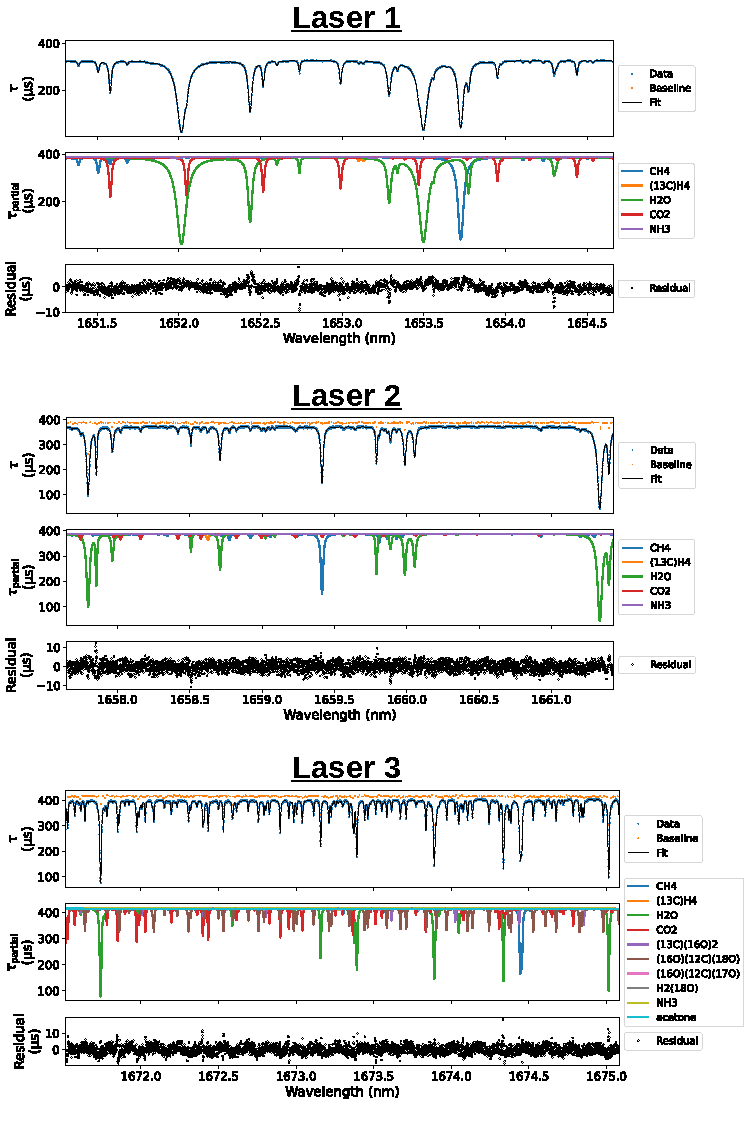
\includegraphics[width=.9\linewidth]{diagrams/crds_laser_results}
		\caption{Typical spectra obtained with the three diode lasers listed in Table \ref{table:crds_diodes}. The spectra measured with laser 1 and laser 3 are of a breath sample. In these measurements, it can be seen that the large concentration of water vapor and carbon dioxide is detected along side the trace gas methane, showcasing the dynamic range of such measurements. The spectrum measured by laser 2 is that of ambient air, where it can be seen that methane is easily detected.}
		\label{fig:crdslaserresults}
	\end{figure}
	
	
	\chapter{CHARACTERIZATION OF THE NIR ACETONE ABSORPTION} \label{chap:acetone}
	Data regarding acetone absorption cross-sections in the NIR region remain scarce, particularly for measurements performed within gas mixtures. This chapter addresses this lack of spectroscopic references by presenting acetone cross-section measurements that exhibit a higher signal-to-noise ratio than those previously reported in the literature. Furthermore, we propose an empirical model for the acetone cross-section that remains valid across a wavelength range suitable for breath characterization via NIR spectroscopy. Collectively, these results significantly advance the capability of acetone concentration characterization using NIR absorption spectroscopy.
	
	The spectroscopic detection of acetone is critical across several scientific disciplines. In the medical domain, it has attracted significant interest due to acetone's potential as a biomarker for conditions such as type-1 diabetes (T1D), type-2 diabetes (T2D) \cite{Wang_2013}, and heart failure \cite{Marcondes_Braga_2020, Marcondes_Braga_2012}. It is also utilized to monitor patients with ketoacidosis \cite{Wang_2013, Owen_1982} or those adhering to high-fat ketogenic diets \cite{Stafstrom_2004}. In healthy individuals, typical concentrations of acetone in exhaled breath range from 0.2 ppm to 1.03 ppm, whereas levels in T1D patients can elevate to 1.7–3.8 ppm or higher \cite{Wang_2013}. Conversely, atmospheric acetone concentrations are typically much lower, ranging from 1–10 ppb \cite{Singh_1994, Schade_2006}, necessitating even more sensitive techniques for environmental monitoring. Beyond medical applications, the spectroscopic analysis of acetone is also essential in astronomical observations \cite{Snyder_2002, Lykke_2016}.
	
	In the NIR, acetone exhibits a relatively broad absorption band peaking at 1672.44 nm \cite{pnnl_database_gas_phase}. This broadband absorption is illustrated in Fig. \ref{fig:acetone_PNNL_data}a), while Fig. \ref{fig:acetone_PNNL_data}b) provides a magnified view of the NIR absorption cross-section, including an inset that highlights the peak of this absorption feature. The structure shown in the inset is of particular interest because it can be resolved using the tuning range of a typical distributed feedback (DFB) diode laser. It is this feature that we will first characterize.
	
	\begin{figure}[H]
		\centering
		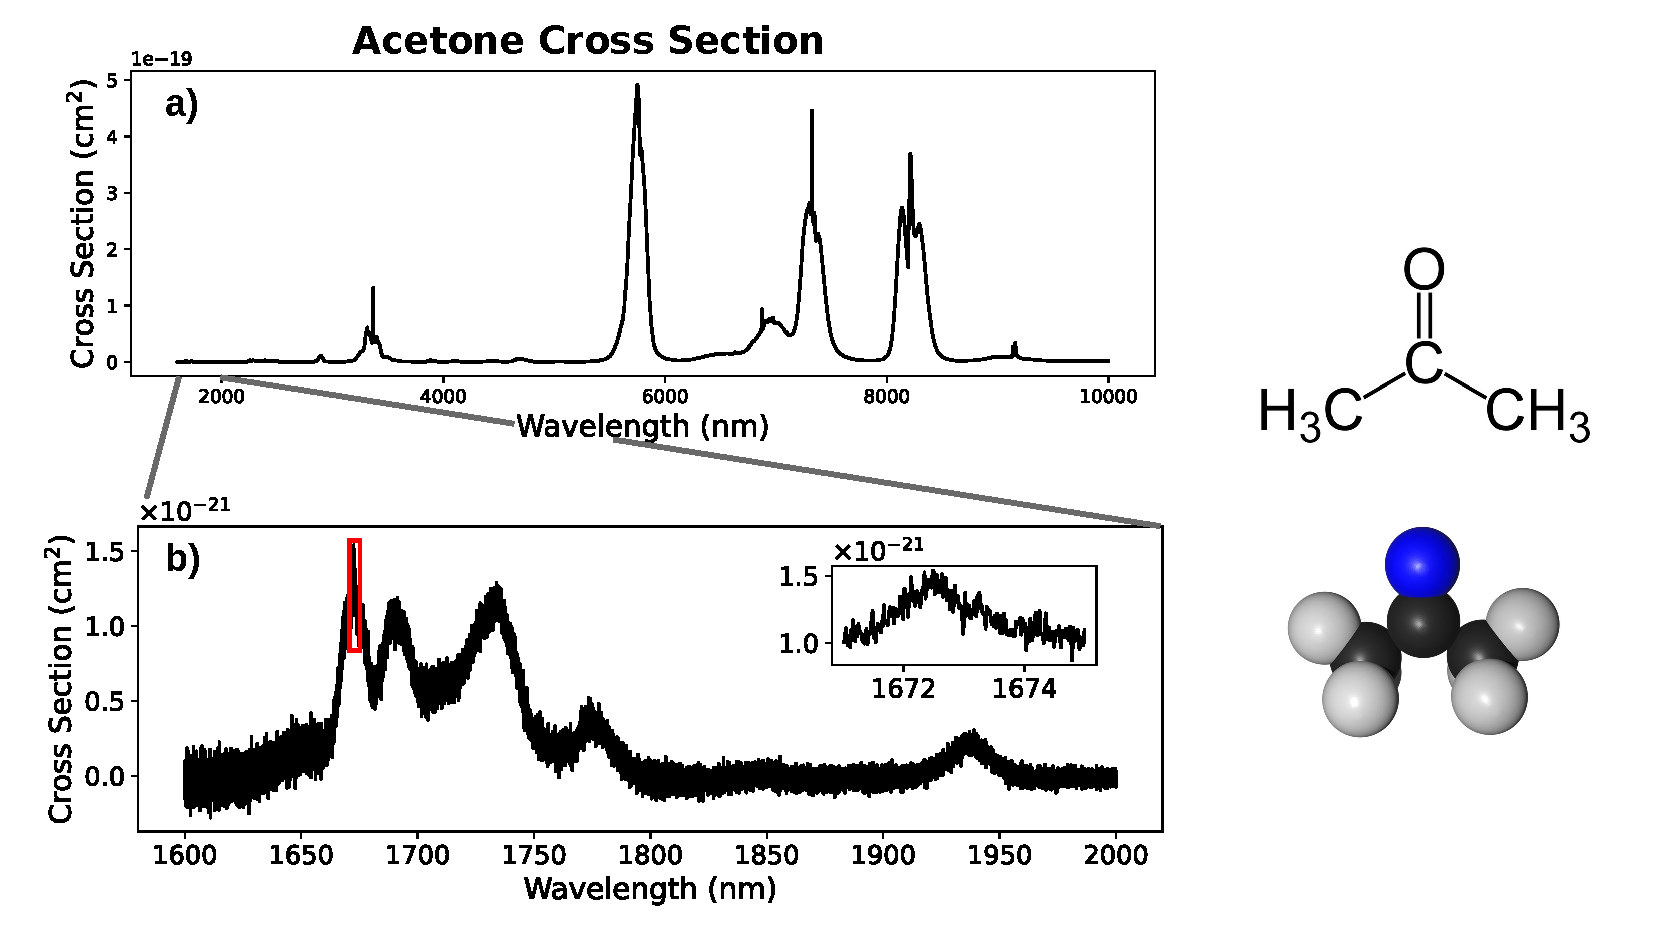
\includegraphics[width=1.0\linewidth]{diagrams/acetone_PNNL_plots}
		\caption{Absorption spectrum of acetone in the NIR plotting the data from the Pacific Northwest National Lab (PNNL) Gas-Phase Databases for Quantitative Infrared Spectroscopy \cite{pnnl_database_gas_phase, pnnl_isobutane}. The shown spectrum is a composite of 10 different measurements of different concentrations of acetone vapor back filled with nitrogen to $760\pm5$ Torr taken with a Bruker-66V FTIR spectrometer.}
		\label{fig:acetone_PNNL_data}
	\end{figure}
	
	As discussed in Ch. \ref{chap:fitting_spectra}, the absorption value $\alpha(\lambda)$ for a particular wavelength $\lambda$ is given in terms of the optical cross section value $\sigma(\lambda)$ at that wavelength value and $n$, the number of molecular absorbers per unit volume. This was given as equation (\ref{alpha_n_sigma}) which is repeated here
	\begin{equation} \label{acetone_n_sigma}
		\alpha(\lambda) = n \sigma(\lambda)
	\end{equation}
	
	Determination of the optical cross section magnitude is usually performed by measuring absorption and dividing by the number density, which is determined externally. For the determination of number density, we rely on calibrated mixtures of acetone vapor (supplied by GasCo) which have their concentrations measured in a manner which is NIST-traceable. By knowing the pressure of this gas mixture inside of our measurement chamber, we can determine the number density $n$ of acetone molecules inside the chamber. To minimize error introduced by the determination of the absorption, we employ cavity ringdown spectroscopy (CRDS) to provide a calibration-free measurement of the absorption coefficient $\alpha(\lambda)$. This allows us to avoid errors introduced by the drift of the illumination spectrum between measurement of the baseline intensity $I_0(\lambda)$ and the absorbed intensity $I(\lambda)$. Such errors tend to plague measurements using broadband illumination sources.
	
	Determination of the spectral shape of the absorption cross section $\sigma(\lambda)$ will be done in two phases. The first phase will measure a relatively narrow region of 1671.5-1675nm which encompasses the peak shown in the inset of Fig. \ref{fig:acetone_PNNL_data}b). This narrow region falls within the tuning range of a single DFB diode laser, and we can therefore employ CW-CRDS with this laser on this peak. This has the advantage of allowing a calibration-free measurement of the absorption and therefore an accurate measurement of the magnitude of $\sigma(\lambda)$ in this region. The second phase of measurement will use a broadband frequency comb to determine the broadband shape of the acetone absorption cross section across a greater span of wavelengths. The absorption obtained by these measurement can be scaled to the cross section value using the known cross section values near the peak of 1671.5-1675nm obtained using CW-CRDS.
	
	\section{CW-CRDS in the Region 1671.5-1675nm} \label{sec:acetone_peak}
	This investigation of the acetone absorption peak in the 1671.5–1675 nm NIR region is published in \cite{mine_acetone}; it currently represents the highest-resolution and lowest-noise measurement of the acetone cross-section reported to date for this spectral range.
	
	The shape and magnitude of this absorption peak of acetone have been measured for pure gas samples and those diluted with laboratory air at low pressure (see references in Table \ref{tbl:compare_lit}). However, it has yet to be verified if there are distortions in the spectrum shape occurring at higher pressures, or in the presence of other gas species in cocentrations typical of a breath sample.
	
	The schematic of the experimental setup is shown in Fig. \ref{fig:acetone_crdsexperimentalsetup}, and closely follows the optical layout presented in Fig. \ref{fig:crds_experimentalsetup_nopc} but now includes the laser diode controller (LDC), the acquisition system which consists of a single board computer with onboard analog to digital converter (ADC) and field programmable gate array (FPGA). This acquisition system is shown connected to the AOM driver so that the light incident on the cavity may be rapidly extinguished when the buildup of the cavity output is detected. Additionally we include the high voltage ramp which controls the motion of the piezoelectric transducer (PZT), and the acetone calibration gas as a bottled compressed gas mixture. Directing the operation of the apparatus and recording the data, the computer allows the whole apparatus to be controlled remotely.
	
	\begin{figure}[H]
		\centering
		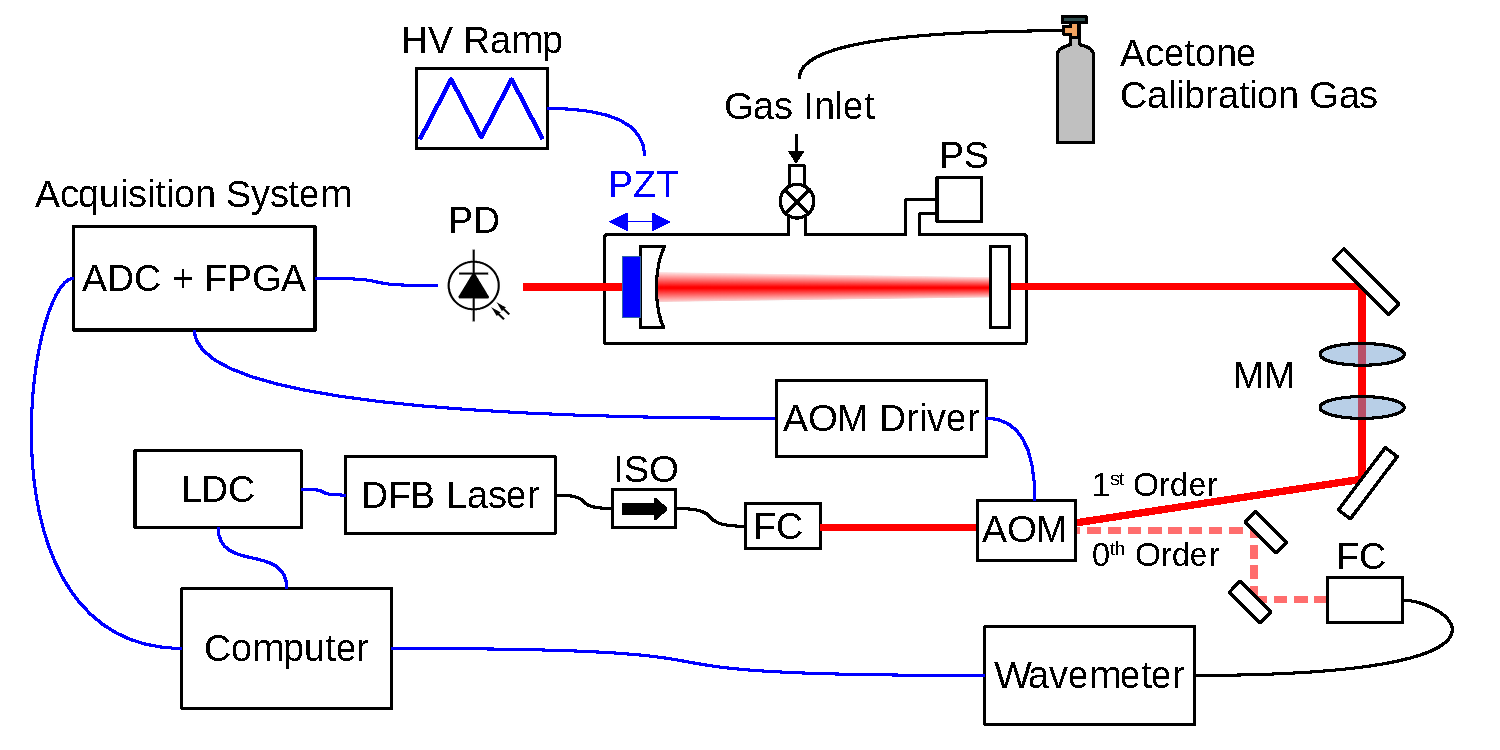
\includegraphics[width=1.0\linewidth]{diagrams/acetone_CRDS_experimentalSetup}
		\caption{Setup of Cavity Ring-down Spectroscopy (CRDS) using a continuous wave laser. The setup includes: distributed feedback (DFB) laser diode, an isolator (ISO), a fiber collimator (FC), an acousto-optic modulator (AOM), switching-off the 1st order deflected beam, a high finesse optical cavity with planar and concave high reflectivity mirrors, a pressure sensor (PS), a piezoelectric actuator (PZT), a laser diode controller (LDC), the acquisition system (ADC + FPGA), and the AOM driver. The zero order beam emerging from the AOM is coupled with a fiber coupler (FC) into a single mode fiber and sent to the wavemeter.}
		\label{fig:acetone_crdsexperimentalsetup}
	\end{figure}
	
	%The 1st order deflected beam is mode-matched to the optical cavity with a mode matching telescope consisting of two planoconvex lenses. The alignment and mode-matching of the cavity were verified by eliminating the presence of higher-order transverse modes. These could be seen by sweeping the length of the cavity using the PZT and monitoring the cavity transmission using the photodiode.
	
	The measurement of the ringdown time is conducted in the manner described in Sec. \ref{sec:crds_ringdown_meas}. Described briefly, the cavity is always scanning in length which allows the laser to periodically resonate with the cavity. During such an event, a buildup in the cavity output light is detected which triggers the shutoff of the incident light. After the shutoff, the acquisition system records the exponentially decaying light, fits the model function \ref{crds_model_exponential} to the recorded curve, and gives a value for the ringdown time $\tau$.
	
	The scan of the spectrum is accomplished by first setting the temperature and current of the laser diode, which in turn sets the operating wavelength of the laser. The tuning profile for the laser used in this work is plotted in Fig. \ref{fig:det_detuningsurface}. After setting the laser parameters, the system is set to wait a set amount of time which was $\sim$1 sec for current changes and $\sim$10 sec for temperature changes. This wait time is to allow the laser to settle into the new operating point, the time scale for these changes were measured in Sec. \ref{sec:crds_tuning_speed}.
	
	After the laser is allowed to settle into its new operating point, the system begins recording ringdown times. A set number of ringdown events is captured at the wavelength, allowing for averaging of the ringdown time values. At the end of the ringdown time acquisitions, the wavelength of the laser is measured by triggering the delay scan of a Michelson interferometer (shown in Fig. \ref{fig:acetone_crdsexperimentalsetup} as Wavemeter). The wavelength is measured using the method of Sec. \ref{sec:wl_wavelength}, where the scan data is split up into 5 separate measurements which yield 5 measurements of wavelength. The median value of these numbers is used to report the final wavelength of the scan point. By conducting the wavelength measurement at the end of the ringdown acquisition, the laser will have additional time to settle into its final operating wavelength.
	
	For precise control of the gas mixture measured by the cavity ring-down technique, the optical cavity is constructed inside of a vacuum chamber. The pressure of the chamber is monitored by a pressure sensor (PS). Two separate pressure transducers are used; one is a diaphragm-type pressure gauge (Vacuum Research 902321), providing a measure of the total pressure inside the chamber which is independent of gas composition. The other is a thermocouple gauge (Varian 531) used to verify that a pressure of $<10^{-3}$ Torr is obtained when evacuating the chamber using a fore-pump (Leybold, Scrollvac SC15D).
	
	\subsection{Acetone Absorption Measurement Procedure}
	Calibrated gas mixtures of acetone were obtained from GasCo at 5 ppm and 30 ppm. The calibration of the mixtures are NIST-traceable, and the calibration certificates of the mixtures claim 10.02 ppm $\pm$ 2\% and 27.33 ppm $\pm$ 5\%, respectively. We investigate the shape of the NIR absorption spectrum of acetone by measuring the sample of 27.33 ppm calibration gas under various pressures and conditions of dilution, including conditions of human breath samples. 
	
	The chamber was first evacuated and the baseline ring-down time measured. A linear fit of the baseline ring-down time against wavelength is later used to evaluate $\tau_0 (\lambda)$ when the absorption is calculated from (\ref{crds_alpha}). The evacuated chamber was filled with an initial pressure measured on the diaphragm gauge, and the wavelength dependent ring-down time of the cavity was determined by taking the average of 100 separate ring-down measurements conducted at 1000 different wavelengths. The duration of the scans were in the range of 1-2 hours, with spectra containing larger absorptions taking longer due to the decreased light being transmitted from the cavity.
	
	The calibration gas was first measured with minimal dilution to establish that the acetone absorption cross section does not show any detectable pressure dependence in the range 30-141 Torr. Using the same sample of calibration gas, we also investigated the acetone absorption in the range 141-500 Torr by diluting with ambient air. No distortions of the acetone cross section were detectable at these increased pressures.
	
	During this investigation, it was found that the amount of time spent vacuuming the chamber had an effect on the long-term stability of the acetone absorption measurement. This effect is investigated in more detail in Sec. \ref{sec:acetone_drift}. In light of this drift, an optimized procedure was used to minimize the effect and to report the parameters for the acetone cross section in Sec. \ref{sec:coeffs_acetone}.
	
	In Sec. \ref{sec:breath_dilution}, we demonstrate the utility of the acetone cross section model by measuring the acetone concentration in samples of human breath. We further demonstrate the accuracy of this process by diluting these samples with a known amount of calibration gas and showing that the subsequently measured spectrum is consistent with the amount of acetone gas added and the initial measurement.
	
	The ring-down time measurement noise is characterized in Sec. \ref{sec:acetone_det_limit}, and this information is used in \ref{sec:simulation} to simulate the effect of this noise on the spectrum fitting process and quantify the error which is propagated to the final gas concentration determination.
	
	\subsection{Empirical Model of the Absorption Peak}
	We monitored the broadband shape of the NIR acetone absorption feature in the range 1671.5-1675 nm by constructing an empirical model of the peak shape. We give a normalized peak shape $\tilde{\sigma}_{\mathrm{ac}}$ in the form
	\begin{equation} \label{sigma_tilde}
		%\tilde{\sigma}_{\mathrm{ac}}(\lambda) = \Gamma^2(\lambda-p_2)\Big/\left[(\lambda-p_2)^2 + \Gamma^2(\lambda-p_2)\right]
		\tilde{\sigma}_{\mathrm{ac}}(\lambda) = \frac{\Gamma^2(\lambda-p_2)}{(\lambda-p_2)^2 + \Gamma^2(\lambda-p_2)}
	\end{equation}
	where the width parameter $\Gamma(\lambda)$ is given by a linear dependence on wavelength
	\begin{equation}\label{Lambda}
		\Gamma(\lambda) = p_0 + p_1 \lambda
	\end{equation}
	The $p_1$ term characterizes the asymmetry of the peak, and for $p_1=0$ the above function reduces to a symmetric Lorentzian peak. We scale $\tilde{\sigma}_{\mathrm{ac}}(\lambda)$ to an amplitude $c_0$ and offset by a constant $c_1$ to give the model acetone cross section
	\begin{equation} \label{acetone_model}
		\sigma_\mathrm{ac}(\lambda) = c_0\tilde{\sigma}_{\mathrm{ac}}(\lambda) + c_1
	\end{equation}
	The peak of this model cross section occurs at $\lambda=p_2$ with a magnitude $c_0 + c_1$.
	
	The proposed shape of the NIR acetone absorption cross section (\ref{acetone_model}) fits well to experimental data in the wavelength range of this investigation, but gives difficulties when this function must be extrapolated to fit extended wavelength ranges in future investigations. The peak shape function $\tilde{\sigma}_{\mathrm{ac}}(\lambda)$ approaches a constant at large values of $\left|\lambda-p_2\right|$ and has a zero at $\Gamma(\lambda-p_2)=0$. To ammend this, the function $\Gamma(\lambda)$ can be clamped such that a linear behavior is displayed in this wavelength range but then rolls off to a constant value outside of it before encountering the zero of $\Gamma$. These considerations could be used to construct a modified model which extrapolates well, such as the model presented in Sec. \ref{sec:acetone_broadband}.
	
	To model the experimentally observed spectra, we include the effect of water vapor contamination and an imperfect absorption baseline. The calibration gas mixtures used for this measurement were not perfectly pure and contained some additional absorption primarily due to water vapor. This contamination was small in comparison to the desorption of water from the aluminum chamber walls. Due to limitations of the chamber construction, the setup could not be heated to remove this outgassing. It was therefore necessary to separate the contributions from acetone and water vapor absorptions. The need for baseline corrections results from the drift which is discussed in Sec. \ref{sec:acetone_drift}.
	
	In order to fit the experimentally measured spectra of the calibration gas at different pressure values, the following model is used
	\begin{equation} \label{fit_model}
		\alpha(\lambda) = a_0\tilde{\sigma}_{\mathrm{ac}}(\lambda) + a_1 + a_2(\lambda - \lambda_0) + a_3\,\sigma_\mathrm{H_2O}(\lambda)
	\end{equation}
	The $a_{0,1}$ are related to the $c_{0,1}$ cross section parameters by the ideal gas number density $P/k_B T$ and the concentration of acetone $y_\mathrm{ace}$, and similarly, the $a_3$ is related to the concentration of water vapor $y_3$ by
	\begin{equation} \label{ai}
		a_{0,1} = \left(y_\mathrm{ace}\frac{P}{k_B T}\right)\,c_{0,1} \qquad\qquad
		a_{3} = \frac{P}{k_B T} y_{3}
	\end{equation}
	
	The $a_2$ term is included to reduce the effect of drift which tends to tilt the observed spectra when the acetone absorption is slightly drifting. This was necessary for some of the calibration gas measurements since a long-term drift in the acetone absorption was observed (see Sec. \ref{sec:acetone_drift}). The use of this term corresponds to the $B=1$ fitting model discussed in \ref{sec:simulation}, and offers improved immunity to spectrum tilt at the expense of degraded $a_{0,1}$ determination. It was also found that the use of the $a_2$ baseline slope parameter introduced a slight amount of crosstalk with the $p_1$ parameter and hence was not used in the final determination of the cross section parameters. The $\lambda_0$ parameter does not affect the final expanded form of the baseline polynomial $a_1 + a_2(\lambda-\lambda_0)$, but choosing $\lambda_0 =1673.5$ nm in the center of the scan reduced correlation between $a_{1}$ and $a_2$.
	
	The absorption cross section of water $\sigma_\mathrm{H_2O}(\lambda)$ was calculated using the HAPI Python module \cite{HAPI_2016}, which can simulate the absorption cross sections of many atmospheric molecules using parameters in the HITRAN database \cite{hitran_2020}. For these calculations, measurements of the total chamber pressure and temperature are needed. The broadening parameters were initially calculated under the assumption of a dry air mixture, with this assumption iteratively relaxed (Section \ref{sec:self_broading_iteration}).
	
	The fit of the model was performed using Levenberg-Marquardt algorithm to vary the nonlinear model parameters $p_0$, $p_1$, $p_2$, and the wavelength correction factor $\beta = p_\lambda$ from equation (\ref{wl_correction_factor}). For each trial value of these parameters the linear coefficients $a_{0-3}$ of the model absorption were determined using the unweighted linear decomposition procedure (\ref{leastSquares}) .
	
	The fit of equation (\ref{fit_model}) to the observed absorption spectrum yields the concentration of water vapor from the values of $a_{3}$ using the relation of Eq. (\ref{ai}) and the relative contributions of the offset term $a_1$ and the peak amplitude $a_0$. The baseline slope term $a_2$ includes the contribution from a tilt of the spectrum which was attributed to the long-term drift (see section \ref{sec:acetone_drift}) occurring during the course of the acquisition.
	
	The $p_{0-2}$ define the shape of the acetone absorption, and changes in these values are indicative of a changing cross section. In this investigation, we confirmed that the values of $p_{0-2}$ stayed relatively constant and the values of $a_0$ and $a_1$ were linear with acetone number density over a range from 30-500 Torr, indicating that the cross section showed no dependence on pressure. Additionally, we confirmed this behavior in the presence of laboratory air in the range 141-500 Torr.
	
	\subsection{Absorption Linearity in the Range of 30-500 Torr}
	The optical absorption cross section $\sigma(\lambda)$ can in general be dependent on the pressure, temperature, and presence of other gas species. The linearity of the acetone NIR absorption with number density has been established for pure acetone samples in \cite{Wang_2004} in the range $2\times10^{-3}$ to $9\times10^{-2}$ Torr, indicating that the NIR cross section for acetone must, to some degree, be independent of pressure. In this work we extend the range of conditions under which the NIR absorption of acetone is known to be linear.
	
	For pressures in the range 30-141 Torr we investigated the absorption pressure dependence of a sample of dry air mixture 27.33ppm calibration gas. The sample was used as provided from the supplier, preventing dilution by flushing the gas lines several times and evacuating the measurement chamber before filling. The linear behavior of the absorption magnitude is seen from $a_{0,1}$ when plotted against pressure, indicating that there is very little effect of pressure and self-broadening on the absorption cross section.
	
	Shown in Fig. \ref{fig:acetone_crdsfits} are two sequences of acetone calibration gas measurements along with their fits to the model absorption of Eq. (\ref{fit_model}). The pressure was changed by partially evacuating the chamber using the scroll pump. For the measurements shown, the chamber was filled at 120 Torr and 50 Torr. A slight upward tilt of the measured absorption spectrum can be seen on the larger wavelength side of these two measurements, which was later attributed to a long-term drift of the acetone absorption (Sec. \ref{sec:acetone_drift}). The narrow absorptions of water can be seen superposed on the acetone absorption. The values of the coefficients obtained from the fit to the absorption curve are shown as by the points of Fig. \ref{fig:acetone_crdsfits} plotted against pressure.
	
	\begin{figure}[H]
		\centering
		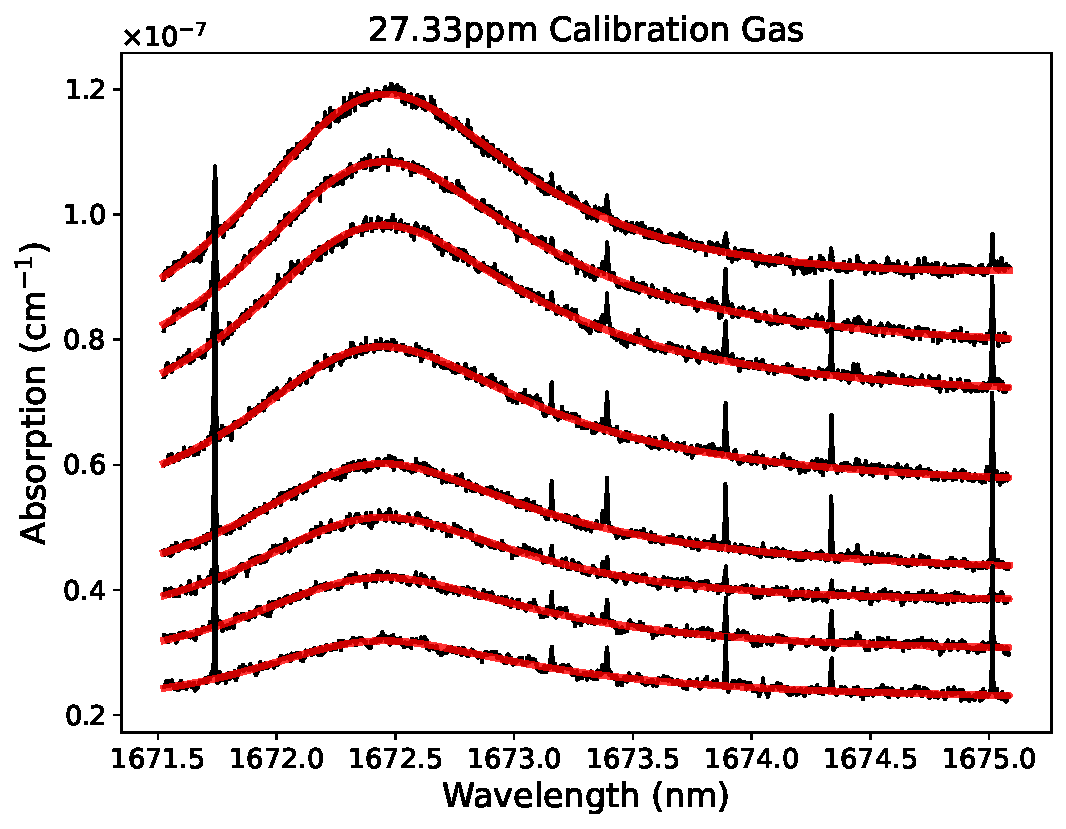
\includegraphics[width=0.8\linewidth]{diagrams/acetone_CRDS_fits}
		\caption{Absorption measurements for 27.33 ppm acetone calibration gas at different pressures. The measured absorption is shown in black the fit to this data is shown in red using the acetone cross section model given by (\ref{fit_model}) with the water vapor contributions (seen as the sharp peaks in the data) subtracted out by setting $a_3$ to zero after the fitting process. The model fits well to the data and shows no direct dependence on pressure. A slight upward tilt of these plots can be seen on the right (where the wavelength scan started) for the 120 and 50 Torr measurements. This was attributed to the drift discussed in Sec. \ref{sec:acetone_drift}. It can be seen that the $a_2$ slope term of the fitting model effectively accounts for these distortions allowing for analysis of the peak shape.}
		\label{fig:acetone_crdsfits}
	\end{figure}
	
	Very little distortion of the peak shape was revealed by the near constant values of $p_0$ and $p_2$ resulting from the fitting, as seen in Fig. \ref{fig:acetone_crdsresults30ppm}. The relatively large variance of $p_1$ is attributed to a coupling with the $a_2$ baseline slope term. Due to the presence of drift, we could not remove the interfering term without detrimentally affecting the fit. Because of this, we did not use the data presented in Fig \ref{fig:acetone_crdsresults30ppm} for the final resolution of the coefficients $p_{0-2}$. This is discussed further in Sec. \ref{sec:coeffs_acetone}. Additionally, this drift resulted in poor control of the calibrated mixture, so we did not use the slope of the fit line (as was done in \cite{Wang_2004}) to resolve the final value for the cross section magnitude.
	
	\begin{figure}[H]
		\centering
		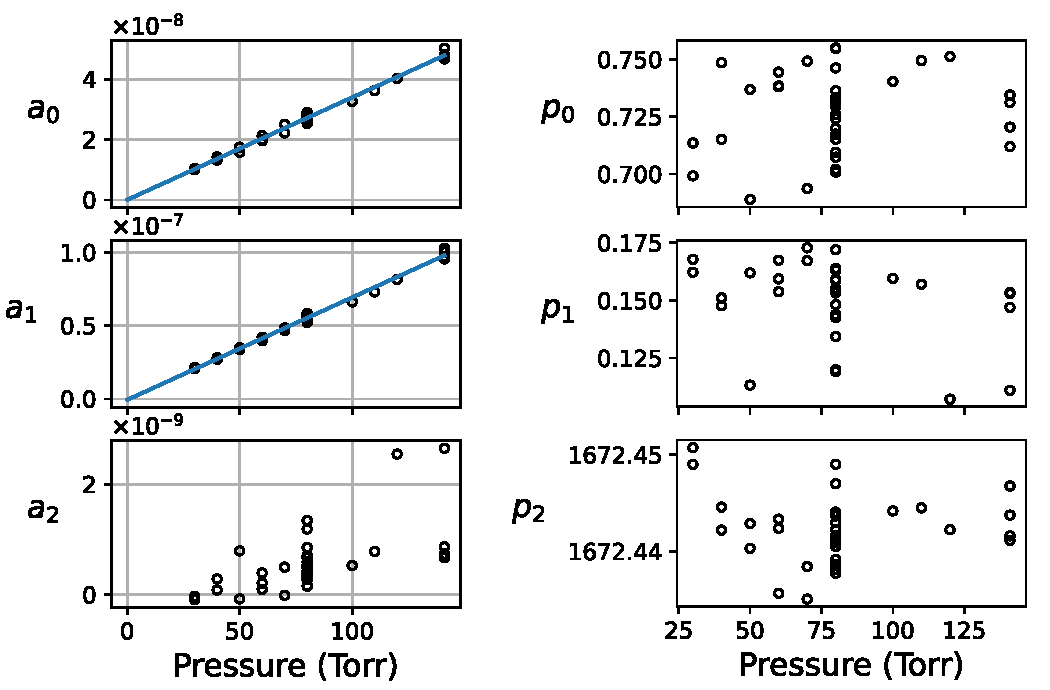
\includegraphics[width=0.85\linewidth]{diagrams/acetone_CRDS_results_30ppm}
		\caption{Coefficients resulting from the fit of Eq. (\ref{fit_model}) to the spectrum measurements of 27.33 ppm calibration gas at pressures 30-141 Torr. The linear behavior of $a_{0,1}$ indicates the non-changing behavior of the acetone cross section with pressure, which is additionally verified by the consistent values of the $p_{0-2}$ coefficients.}
		\label{fig:acetone_crdsresults30ppm}
	\end{figure}

	
	In the range of pressures 141-500 Torr, we further investigated the linearity of the absorption by diluting the same sample of acetone calibration gas using ambient laboratory air in several increments. In this case, diluting the sample does not appreciably change the number density $n$, but only changes the pressure of the measurement environment and introduces contaminants. We therefore expect the absorption magnitudes $a_0$ and $a_1$ of the resulting fit to remain approximately constant as the dilution is performed for a linear absorption.
	
	Indeed $a_0$ and $a_1$ did not show any effect of the dilution and only showed a long-term dependence which is shown in the left panel of Fig. \ref{fig:acetone_crds_resultsairdilution} and resembles the long-term drift behavior further investigated in Section \ref{sec:acetone_drift}. A similar drift behavior can be seen in Fig. \ref{fig:actetone_crds_drifts}a. With the exception of few outliers, the values for $p_{0-2}$ shown in the right panel of Fig. \ref{fig:acetone_crds_resultsairdilution} showed stable behavior indicating that the shape of the acetone peak was unchanging.
	
	\begin{figure}[H]
		\centering
		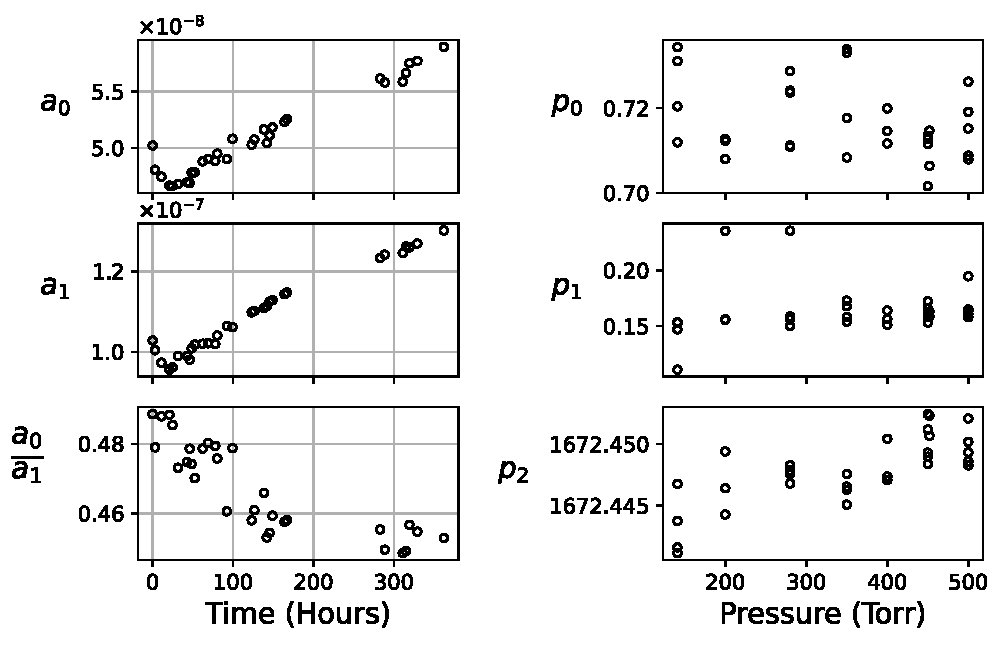
\includegraphics[width=0.9\linewidth]{diagrams/acetone_CRDS_results_airDilution}
		\caption{Air dilution results. 141 Torr of 27.33 ppm calibration gas was diluted with laboratory air over an extended period of time. Due to the linearity of the acetone absorption, no direct correlation with the parameters was observed when pressure was increased. Instead, the main pattern that was observed was the same long term drift that was reported in Sec. \ref{sec:acetone_drift} and Fig. \ref{fig:actetone_crds_drifts}.}
		\label{fig:acetone_crds_resultsairdilution}
	\end{figure}
	
	The only indication that there is some distortion of the peak shape can be seen in the bottom left of Fig. \ref{fig:acetone_crds_resultsairdilution}, where there is a slight fluctuation of $a_0/a_1$. This ratio characterizes the height of the acetone absorption peak to the local offset and is independent of acetone concentration in our model. We attribute this small variation over time to contaminants which result in an apparent broadband and featureless absorption that increases the value of $a_0$ in the fit. This could result from increased scattering as an increasing amount of atmospheric gas is let into the chamber.
	
	\subsection{Drift of the Acetone Absorption} \label{sec:acetone_drift}
	It was determined that the main limiting factor in our spectrum measurements was the apparent drift of the acetone absorption over a span of many hours. Since scans of the spectrum took a period of 1-2 hours this drift was acounted for by using the $a_2$ slope term in the fit equation (\ref{fit_model}). Coupling of this term with the $p_1$ resulted in a degraded ability to resolve the value of this coefficient.
	
	To quantify the nature of the spectrum drift, we choose 5 wavelengths which reside on the acetone feature in between the sharp water features, and a sixth wavelength was chosen to monitor an isolated water peak. The results of two different long-term drift measurements is shown in Fig. \ref{fig:actetone_crds_drifts}. It was found that the time dependence of these absorption values was well modeled by a double exponential function plus a linear term
	\begin{equation} \label{drift_fit}
		\alpha(t) = mt + b + A_1 e^{-t/T_1} + A_2 e^{-t/T_2}
	\end{equation}
	
	In Fig. \ref{fig:actetone_crds_drifts}, two different drift measurements are shown in panes (a) and (b) and compared in pane (c). The preparation of the sample was nearly identical in both cases except for the amount of time spent by the chamber under low vacuum prior to acetone calibration gas introduction. In (a), the chamber had been continuously pumped for six hours after the thermocouple gauge had reached its minimum reading of 0.001 Torr, and in (b) the chamber was only pumped down to 0.1 Torr. A much greater defect between the initial absorption value and that obtained roughly 20 hours later is observed in the conditions of (a). It should be noted that the value of peak acetone absorption predicted by other measurements listed in Table \ref{tbl:compare_lit} agree most closely with this initial absorption value. In light of this finding we decided to conduct the measurements for the coefficients in Table \ref{table:acetone_coeffs} under the conditions of (b), where the defect is smallest.
	
	\begin{figure}[H]
		\centering
		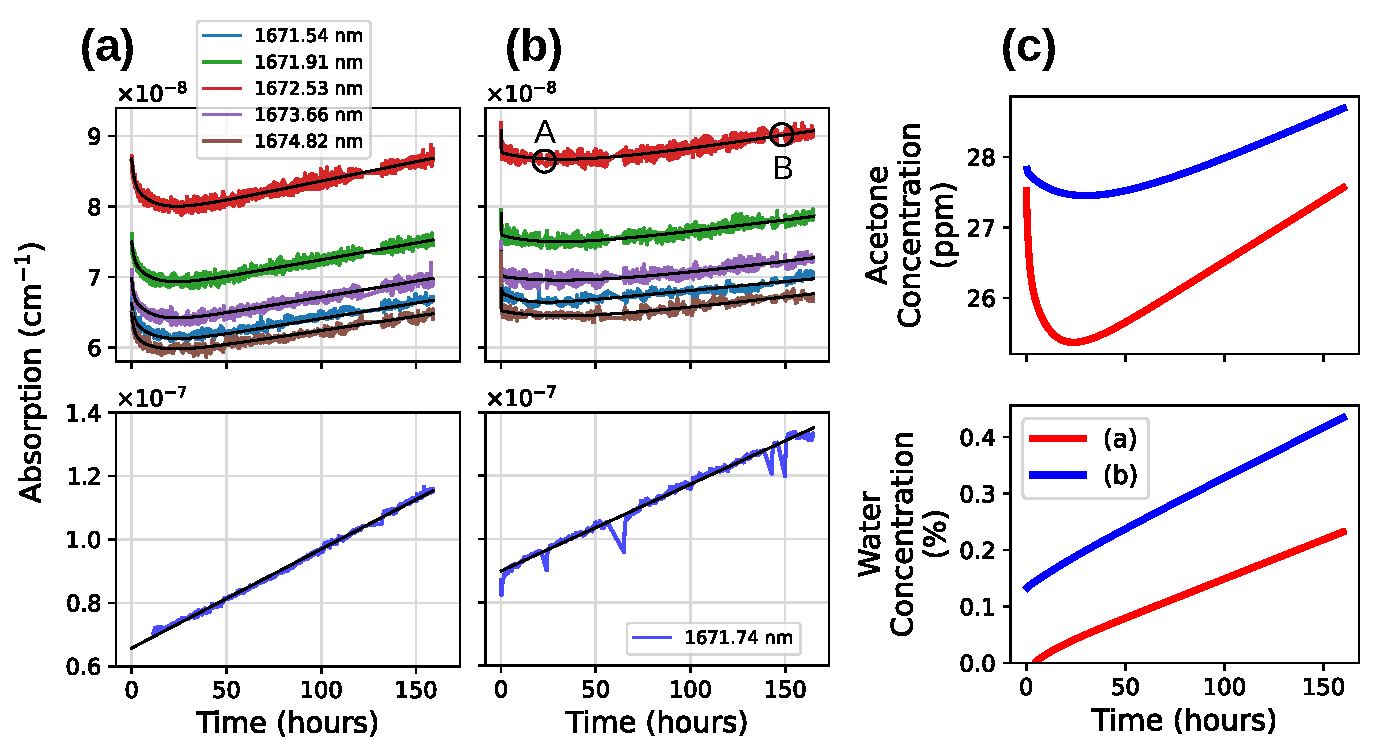
\includegraphics[width=1.0\linewidth]{diagrams/actetone_crds_drifts}
		\caption{Shown in (a) and (b) are long-term measurements of similar samples of calibration gas which had been loaded into the chamber with differing amounts of prior vacuum desiccation of the chamber walls. In (a) the chamber was actively vacuumed for over six hours prior to loading the sample, and in (b) the chamber was only vacuumed long enough to reach 0.1 Torr. In the tops of (a) and (b) are absorption measurements at five different wavelengths corresponding to points on the acetone absorption profile intentionally chosen to avoid water contributions. The red trace at 1672.53 nm is near the peak acetone absorption. In the lower plots of (a) and (b), absorption measurements of the water peak near 1671.74 nm are shown during the same time. Shown with the black circles in (b) are two spectrum measurement points where the drift is minimized and nearly linear. The black curves are fits to the absorption measurements, and these six curves are evaluated at selected times to give absorption measurements at the six measurement wavelengths. Using Eq. \ref{leastSquares}, these absorptions are converted to concentrations of water and acetone and the results are shown in pane (c), where the two different measurement conditions are compared.}
		\label{fig:actetone_crds_drifts}
	\end{figure}
	
	For each wavelength in the drift measurement, we fit a curve to the absorption coefficient over time using equation (\ref{drift_fit}). The water absorption was fit using a simple linear equation. The fit equations are shown as black curves in panes (a) and (b) of Fig. \ref{fig:actetone_crds_drifts}. The evaluation of these curves was used to check for distortions of the acetone absorption profile.
	
	We additionally used the model drift equation (\ref{drift_fit}) to evaluate 5 different absorption values from which a fit of $p_1$, $a_0$ and $a_1$ was obtained. This was done to eliminate the considerable time required for the laser to fully stabilize to a new wavelength, as evaluating the temporal fit equation allows us to know the absorption at several wavelengths simultaneously. To recover the shape of the acetone absorption, $p_0$ and $p_2$ were held fixed and $a_2$ was held at zero. This 3-parameter model was used to fit to the five different acetone probe points to monitor for changes of the peak shape during the time evolution of the spectrum. It was found that the value of $p_1$ extracted from these fits then became stable and all of the spectrum evolution was contained in $a_0$ and $a_1$, which seemed to vary together keeping the ratio $a_0/a_1$ nearly constant. This indicates that the acetone absorption evolved as a scale factor, and the drift is most likely due to a changing number density of acetone, and not a distortion of the NIR peak.
	
	Under the assumption that the change of the acetone absorption profile is due to a changing acetone concentration, Fig. \ref{fig:actetone_crds_drifts}(c) was constructed from the measurements shown in panes (a) and (b). For a set of chosen times in the measurement interval, the fit equations to the changing absorption were evaluated to yield six absorption measurements at six known wavelengths. These were used to set up the sytem of equations (\ref{fit_spectrum}) to be established from which the concentrations of acetone and water vapor could be solved using (\ref{leastSquares}). By repeating this procedure for many selected times in the measurement interval, we construct the curves shown in Fig. \ref{fig:actetone_crds_drifts}(c).
	
	From Fig. \ref{fig:actetone_crds_drifts}(c) we see that in the first 20 hours, the drift is much more severe for the case where the chamber walls were dried with vacuum desiccation prior to sample introduction. Due to the long time scale, we attribute the drift to an interaction of acetone with the aluminum walls of the chamber, but this requires further investigation. The chamber in our case was rather large, having the shape of a rectangular prism of approximate internal dimensions 9 $\times$ 13 $\times$ 176 cm.
	
	
	\subsection{Determination of Model Coefficients} \label{sec:coeffs_acetone}
	
	Determination of the cross section coefficients was performed by fitting the model
	\begin{equation} \label{fit_model_coeff}
		\alpha(\lambda) = a_0\tilde{\sigma}_{\mathrm{ac}}(\lambda) + a_1 + a_2\,\sigma_\mathrm{H_2O}(\lambda)
	\end{equation}
	to the absorption measurments conducted at the relatively stable laboratory temperature of 21.8 $^\circ$C, as measured by an AccuRite Iris weather station located in the lab. It was found that the slope term contained in (\ref{fit_model}) was not necessary for achieving a good fit to the data when the drift was minimized. The above model gave improved stability of the $p_1$ coefficient contained in the $\tilde{\sigma}_{\mathrm{ac}}$ term and is equivalent to the $B=0$ model simulated in \ref{sec:simulation}. The resulting fit parameters allow the offset $a_1$ and peak amplitude $a_0$ to be determined independently which correspond to $c_{0,1}$ through (\ref{ai}).
	
	In determining the values in Table \ref{table:acetone_coeffs}, care was taken to evaluate only spectra which had been taken in the minimum of the temporal variation observed in Fig. \ref{fig:actetone_crds_drifts}. This point is marked by the black circle marked A in pane (b). At this point the tilt of the spectrum induced by the drift of the acetone absorption is minimized and we can uniquely determine the spectrum shape. Additionally, we analyzed data collected in the linear portions of the drift with the wavelength scan conducted in a back-and-fourth motion, allowing the relatively slow drift to make roughly equal and opposite contributions across the scan. Such a point is marked B in Fig \ref{fig:actetone_crds_drifts}(b).
	
	The shape of the spectrum was not found to show any dependence on pressure or the presence of other species under the conditions that were investigated. Since the coefficients of this model resulting from the fitting procedure gave stable values, we simply took an average of the results to report the numbers in Table \ref{table:acetone_coeffs}.
	
	\begin{table}[H]
		\begin{center}
			\caption{ Values of the coefficients resulting from the fit of the acetone cross section at $T=21.8$ $^\circ$C. The peak of the model acetone cross section is given by $a_0 + a_1 \sim 1.22 \pm 0.01\;\mathrm{cm}^2$}\label{table:acetone_coeffs}
			\begin{tabular}{|c|c|c|c|}
				\hline
				\textbf{Coefficient} & \textbf{Value} & \textbf{Uncertainty} & \textbf{Unit} \\
				\hline
				$c_0$ & $3.92\times10^{-22}$ & $0.05\times10^{-22}$ & $\mathrm{cm}^2$ \\
				\hline
				$c_1$ & $8.3\times10^{-22}$ & $0.1\times10^{-22}$ & $\mathrm{cm^2}$ \\
				%\hline
				%$c_2$ & $2.990\times10^{-5}$ & & cm$^2$ \\
				\hline
				$p_0$ & $0.704$ & 0.002 & nm \\
				\hline
				$p_1$ & $0.174$ & 0.002 & unitless \\
				\hline
				$p_2$ & $1672.442$ & $0.001$ & nm \\
				\hline
			\end{tabular}
		\end{center}
	\end{table}
	
	\subsection{Measurements With Diluted Breath Samples and Breath Dilution Procedure} \label{sec:breath_dilution}
	
	We demonstrate that the concentration of acetone can be recovered from the NIR spectrum of a breath sample using the acetone model cross section (\ref{acetone_model}) with coefficient values from Table \ref{table:acetone_coeffs}. We first measure the absorption spectrum of a breath sample, dilute this sample with a known amount of acetone calibration gas, and then measure the absorption spectrum again. If the concentration of acetone is accurately recovered from the two breath samples, then the concentrations obtained from the two spectra should be consistent with the known dilution.
	
	A pressure around 70 Torr was found to be the optimum to measure breath samples in our apparatus in this wavelength range. A higher sample pressure would cause the water peaks to saturate the measurement such that $\tau \rightarrow 0$, resulting in the cavity producing nearly zero transmission signal. Operating just before this point allows for the highest signal to noise ratio of the observed signal while still fully capturing the large water absorptions.
	
	We first filled the chamber (after the baseline $\tau_0(\lambda)$ is characterized) with a breath sample to 70 Torr and measured the spectrum. The cavity was then partially evacuated to 65 Torr and then diluted with calibration gas to the original pressure of 70 Tor. To transfer the breath sample to the measurement chamber, the volunteer is asked to fill a latex balloon, which is then temporarily sealed with a binder clip. This balloon is placed in a refrigerator for approximately 15 minutes to quickly reduce the temperature of the sample. This is done to prevent condensation on the inside of the chamber and gas lines, since fresh breath gas is warmer than the 21.8 $^\circ$C laboratory environment. The final transfer to the evacuated measurement chamber was performed by attaching the baloon to a 1" KF connector and opening a needle valve in a controlled manner to avoid disturbing the optics. The chamber filling rate can be monitored with high sensitivity by monitoring the positions of the cavity resonances in the scan of the PZT (shown in Fig. \ref{fig:acetone_crdsexperimentalsetup}), since the refractive index of the gas changes monotonically with pressure. The final filling pressure is determined using the diaphragm gauge.
	
	The measurements of both the diluted and un-diluted spectra were conducted at 1,000 different wavelengths with 100 averages each. This number of averages is smaller than the optimum (see Sec. \ref{sec:acetone_det_limit}) but this smaller number of averages enabled a faster scan, limiting the effect of the drift mentioned in Sec. \ref{sec:acetone_drift}. This smaller number of averages also places our measurement in the regime of Gaussian white noise (the linear portion of Fig. \ref{fig:acetone_crds_detectionlimit}b), which enables a more direct comparison with the simulation results shown in the Appendix Sec. \ref{sec:simulation}.
	
	The concentrations of the various gas species recovered from the fitting procedure are shown in Table \ref{table:acetone_CRDS_concentrations} for the sample shown in Fig. \ref{fig:acetone_crds_breathplusacetone} before and after the dilution. The calibration gas used for the dilution was measured to contain only a trace amount $<$0.01 ppm of methane and $<$100ppm water. The pre-dilution concentrations recovered from the fit are used to compute the expected concentrations resulting from a dilution with pure acetone calibration gas and these are shown in the fourth column of Table \ref{table:acetone_CRDS_concentrations} and compared to the values resulting from the spectrum fit of the diluted gas.
	
	
	\begin{figure}[H]
		\centering
		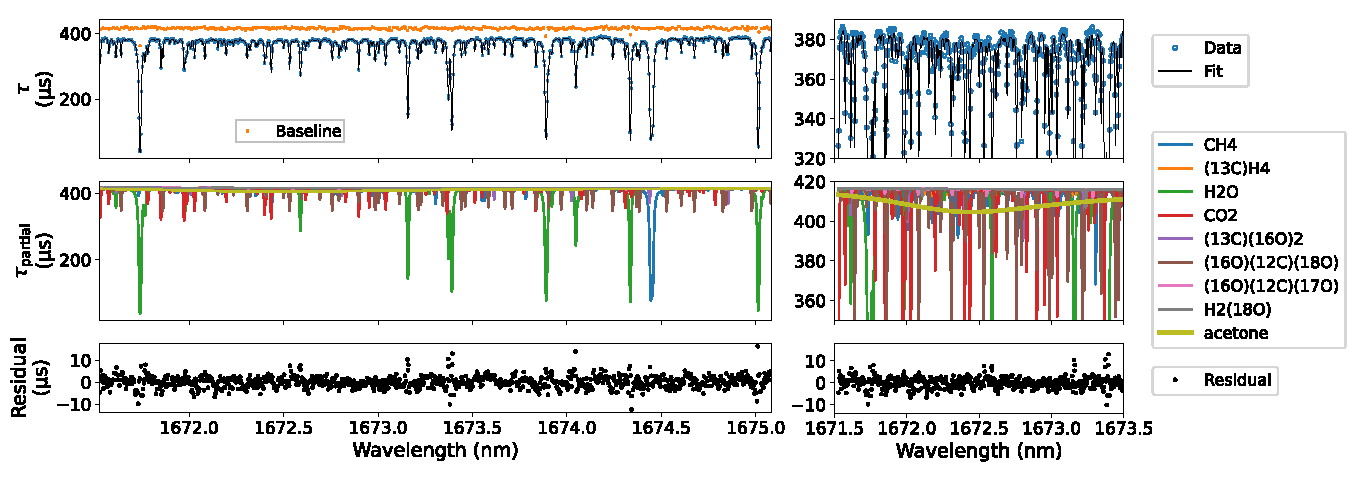
\includegraphics[width=1.0\linewidth]{diagrams/acetone_CRDS_breathPlusAcetone}
		\caption{Shown is a breath sample which has been diluted from 65 Torr to a total of 70 Torr using 27.33 ppm acetone calibration gas. On the left the entire measured breath spectrum is shown alongside the baseline measurement and fit. The species included in the fit are shown graphically in the middle graphs and are plotted by showing the theoretical ring-down response for each species in isolation. The concentrations recovered from the fit of this spectrum are tabulated in the third column of Table \ref{table:acetone_CRDS_concentrations} and show good agreement with the values expected from the dilution. On the bottom the residual is calculated as the difference in the measured ring-down time from the fit equation showing good agreement. The plots on the right are enlarged to show the small contribution from the acetone absorption.}
		\label{fig:acetone_crds_breathplusacetone}
	\end{figure}
	
	\begin{table}[H]
		\caption{Results for breath samples diluted by calibration gas. The breath was intially measured at 70 Torr resulting in the pre-dilution concentrations shown in the second column. The breath sample was then reduced in pressure to 65 Torr using a vacuum pump, and then diluted with 27.33 ppm calibration gas until the total pressure again reached 70 Torr. After this final dilution the spectrum was measured again resulting in the post-dilution concentrations in the third column. The fourth column shows the concentrations which are expected of the post-dilution if the initial concentrations are accurate. The percent fractional change from these expected numbers are shown in the last column. The final diluted breath spectrum is shown in Fig. \ref{fig:acetone_crds_breathplusacetone}.}
		\begin{center}
			\begin{tabular}{|c|c|c|c|c|}
				\hline
				\textbf{Gas} & \textbf{Pre-Dil.} & \textbf{Post-Dil.} & \textbf{Expected} & \textbf{Deviation} \\
				%& \textbf{concentration} & \textbf{concentration} \\
				\textbf{Species} & \textbf{(ppm)} & \textbf{(ppm)} &  & \textbf{(\%)} \\
				\hline
				CH$_4$ 			       & 7.34 & 6.74 & 6.32 & 6.57\%\\ 
				\hline
				$\mathrm{(^{13}C)H_4}$ & 0.092 & 0.088 & 0.080 & 11.6\% \\ 
				\hline
				H$_2$O &                 21730 & 20940 & 18740 & 11.7\%\\
				\hline
				CO$_2$                 & 31400 & 28600 & 27000 & 5.8\%\\ 
				\hline
				$\mathrm{(^{13}C)O_2}$ & 344   & 300 & 296 & 2.7\%\\ 
				\hline
				$\mathrm{CO(^{18}O)}$  & 128.0 & 119.5 & 110.3 & 8.27\%\\ 
				\hline
				$\mathrm{CO(^{17}O)}$  & 24 & 24 & 21 & 17\%\\
				\hline
				$\mathrm{H_2(^{18}O)}$  & 32 & 36 & 28 & 29\%\\
				\hline
				\textbf{Acetone}       & 0.34 & 2.31 & 2.29 & \textbf{0.74}\%\\ 
				\hline
			\end{tabular}
		\end{center}
		\label{table:acetone_CRDS_concentrations}
	\end{table}
	
	\subsection{Single-Wavelength Detection Limit} \label{sec:acetone_det_limit}
	We can evaluate the detection limit of our system by the fluctuations in the measured ring-down time \cite{allan_variance_mod} near the baseline. For a weak absorption, the measured ring-down time $\tau$ is nearly that of the empty cavity baseline $\tau_0$, and must be distinguished from the intrinsic fluctuations of the measurements.
	
	When the measurement is conducted, many averages of the ring-down time are taken at each wavelength to effectively reduce the deviation $\Delta \tau$ of the measurements. However, this cannot be continued indefinitely due to drift. The modified Allan variance \cite{allan_variance_mod} can be used to determine the optimum averaging time and the minimum possible value of $\Delta \tau$ that can be obtained through averaging. This allows the minimum detectable absorption to be determined. Equivalently, we can calculate the Allan variance directly from measurements of the absorption coefficient to give directly the minimum variance of absorption coefficient $\Delta \alpha$. This is shown in Fig. \ref{fig:acetone_crds_detectionlimit}, where the minimum of the modified Allan deviation of the absorption coefficient gives the (1$\sigma$) minimum detectable absorption. For 15.8 seconds of averaging time, we obtained a detection limit of $1.1\times 10^{-10}$ cm$^{-1}$. This corresponds to an acetone concentration of 44 ppb at 70 Torr when the absolute value of the peak absorption cross section is considered, and 134 ppb when just the height of the characteristic peak is considered.
	
	\begin{figure}[H]
		\centering
		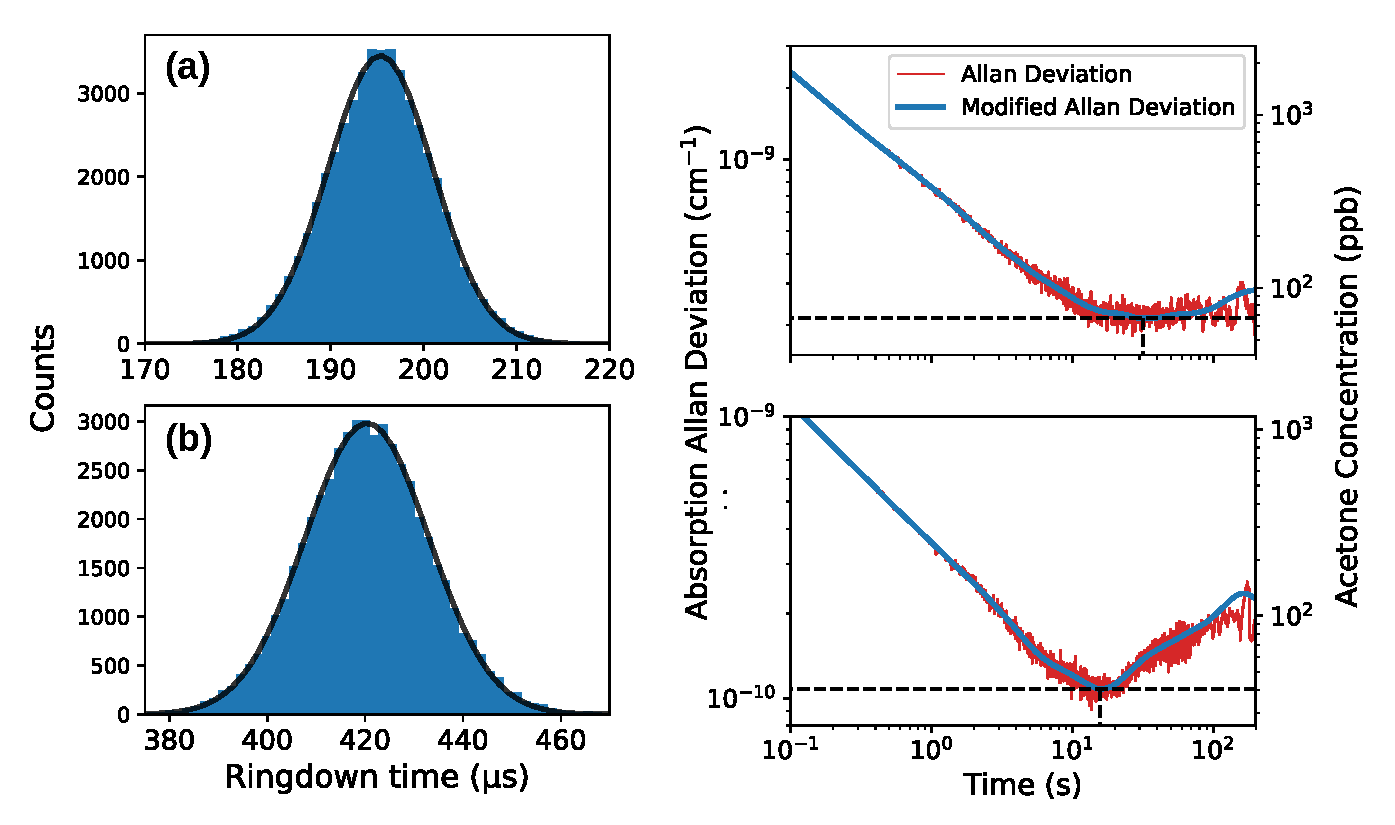
\includegraphics[width=1.0\linewidth]{diagrams/acetone_CRDS_detection_limit}
		\caption{Statistics of ring-down measurements. Here we show two continuous measurements at two concentrations of acetone calibration gas, (a) and (b). The histograms of these measurements are shown in the left pane, along with a Gaussian fit to the bin centers. The wavelength is near the peak acetone absorbance and the measurement shown in (a) is of 27.33 ppm calibration gas at 80 Torr. The measurement shown in (b) is of the empty chamber. The mean ring-down time in (a) is 195 \textmu{}s with standard deviation 5.9\textmu{}s, and for (b) the mean ring-down time is 421\textmu{}s and the standard deviation is 13.1\textmu{}s. The relative deviation $\Delta\tau/\tau$ is approximately 3\% in both cases. On the right the Allan deviation plots is shown alongside the results of the modified algorithm \cite{allan_variance_mod}. The minimum of the modified Allan plot using the data from (b) is used to determine a minimum detectable absorption of $1.1\times 10^{-10}$ cm$^{-1}$ at an averaging time of 16 seconds. The minimum is greater in (a) because this minimum detectable absorption change sits on top of an already relatively large absorption. The right vertical axis shows the equivalent acetone absorption at 70 Torr calculated using the maximum value of the cross section. The linear region on the left of the Allan plots has slope very near $-1/2$ in both cases, which is indicative of Gaussian noise.}
		\label{fig:acetone_crds_detectionlimit}
	\end{figure}
	
	\subsection{Multi-Wavelength Detection Limit}
	It was seen in the previous section that the Allan deviation allows the determination of the smallest possible deviation of the ringdown time measurement $\Delta \tau$, which gives the single wavelength detection limit. We now extend the discussion from a single wavelength concentration uncertainty to the concentration uncertainty of several species concentrations determined simultaneously from a multi-wavelength spectrum scan.
	
	For gas samples which have species which obey the non-interacting gas approximation from Sec. \ref{sec:non_interacting_gas}, the concentrations of these species are determined from a set of measurements of the absorption coefficient and wavelength through the use of (\ref{leastSquares})
	
	\subsection{Discussion}
	The overtone absorption bands, as the C-H stretch band that we investigate in this paper, appear due to anharmonicity \cite{Sandorfy_1978}. The overtones with relatively high transition frequencies, observed in the NIR region involve primarily small mass hydrogen atoms coupled with larger atoms \cite{Weyer_2006}.
	
	The profiles of the overtone absorption bands often show similarity with the profiles of the corresponding bands of fundamental wavelength. Indeed, the fundamental band \cite{Harrison_2011_3um} around $\nu_f$=3320 cm$^{-1}$ and the overtone absorption band that we are investigating around $\nu_0=5979$ cm$^{-1}$ both show a central peak on an elevated base. The fact that $\nu_0 < 2\nu_f$ is reflecting the  anharmonicity, which leads to the frequency of the overtone being smaller that the corresponding multiple of the fundamental frequency. This was used for the determination of the molecular structure from spectroscopy of overtones \cite{Henry_1987}. The assignment of the observed band to the first overtone 2$\nu_a$ of the asymmetric stretching vibration of the methyl group CH$_3$ of acetone with certainty follows from previous research \cite{Pearle_2008, Wang_2004, Hanazaki_1985}.
	
	Our determination of the absorption cross section is based on formula of Eq. (\ref{leastSquares}) and is not relying on the known cross section of acetone for a different absorption band (in UV) as in Ref. \cite{Pawel_2007}. Strictly speaking, Eq. (\ref{fit_model}) determines the total attenuation cross section which includes also losses due to scattering. To the scattering losses contribute all gas components that are present in the optical cavity. However. the scattering cross section at the used wavelengths is many orders of magnitude smaller than the absorption cross section \cite{Penndorf_1957} and can be neglected. We note that the absorption from hot band transitions \cite{Levine_2014_quantum_chem} at our temperature is also negligible.
	
	We performed measurements with a mixture of gases and used the well known absorption cross sections of methane, water and carbon dioxide in the NIR region. The relatively high concentration of acetone and methane compared to other VOCs and high spectral resolution allowed to accurately determine their concentrations in gas mixtures of exhaled breath. The peak value of the acetone NIR cross section and position of the peak absorption for the investigated absorption band are shown in Table \ref{tbl:compare_lit} in comparison to the values obtained in previous research.
	The obtained value of the peak absorption of $1.22\times10^{-21}\text{ cm}^2$ is in good agreement with Refs \cite{Pearle_2008, Wang_2004, Denzer_2010}, and the position of the peak of 1672.4 nm is also in good agreement with Refs \cite{pnnl_database_gas_phase,Pearle_2008}.
	
	\begin{table}[H]
		\caption{ Cross sections and positions of the peak absorption for the stretching 2$\nu_a$ overtone of CH3 group in acetone.}
		\begin{center}
			\begin{tabular}{|c|c|c|}
				\hline
				\textbf{Source} & \textbf{Cross section} & \textbf{Peak Absorption} \\
				& $\sigma$ (cm$^2$) &\textbf{Wavelength} $\lambda$ (nm) \\
				\hline
				This Work \cite{mine_acetone} & $1.22\times10^{-21}$ & 1672.442 \\
				\hline
				\cite{Pearle_2008} & $1.2\times 10^{-21}$ & 1672.15 \\
				\hline
				\cite{Wang_2004} & $1.2\times 10^{-21}$ & 1677.8 \\
				\hline
				\cite{pnnl_database_gas_phase} & $1.4\times 10^{-21}$ & 1672.44 \\
				\hline
				\cite{Denzer_2010} & $1.3\times 10^{-21}$ & 1672.48 \\
				\hline
			\end{tabular}
		\end{center}
		\label{tbl:compare_lit}
	\end{table}
	
	Some variations in the observed absorption and consequently in the retrieved acetone concentration as determined from spectroscopic measurements can be related to equilibration process after the admission of the gaseous sample into the chamber, partial condensation and interactions in the mixture of acetone and water molecules. Such mixtures can show azeotropic behavior \cite{Mahdi_azeotrope}, adsorption effects on condensed fraction and on the walls of the chamber \cite{Duan_1993, CHEN_2001}, and interactions due to hydrogen bonds \cite{COUTINHO_1999, Jean-Joseph_2003, Jean-Joseph_2003_molModels}. These effects can be especially important before the equilibrium is achieved. Indeed, in our measurements the initially observed absorption gradually reduced by about 10\% on a time scale of hours, as seen in Fig. \ref{fig:actetone_crds_drifts}.
	
	Our measurements with diluted samples of the calibration gas show that the achieved detection limit for acetone of 44ppb at 70 Torr total pressure and 15.8 sec integration time is low enough for the analysis of human breath samples, since the typical range of concentrations even for healthy individuals is within 0.2 ppm to 1.03 ppm \cite{Wang_2013}. This is comparable in sensitivity with the MIR sensor employing a 7.32 {\textmu}m quantum cascade laser and a multi pass cell \cite{Li_2023} which demonstrated the detection limit of 21.4 ppb with a 78 s integration time. Note that our sensor does not require any preliminary acetone enrichment or separation as is done for acetone detection with a chemoresistive sensor combined with a catalytic filter and separation column \cite{Bastide_2023}. Despite a relatively narrow measured spectral interval (as compared, for instance, to the frequency comb spectroscopy \cite{ours_review_2022}) it also enables the detection of methane as is shown in Fig. \ref{fig:acetone_crds_breathplusacetone} and Table \ref{table:acetone_CRDS_concentrations}, which often requires a specialized sensor \cite{Kwasny_2023}. The high spectral resolution allowed for the identification of spectral lines contributed by different isotopes, as presented in Table \ref{table:acetone_CRDS_concentrations}. Of particular interest are carbon isotopes for breath analysis \cite{Shao_2022} and for monitoring atmospheric environment \cite{Bakkaloglu_2022}.
	
	\subsubsection{Conclusions}
	We performed cavity ring down spectroscopy of the C-H stretch overtone absorption band in the NIR spectral range of $1671.5-1675.0$ nm. The absorption cross section was determined from the measurements with calibration gas and its mixtures with breath samples. We have shown that a simple empirical model gives good agreement with the absorption cross section of dilute acetone gas in the measured wavelength range. The peak absorption value of $1.22 \times 10^{-21}\text{ cm}^2$ positioned at 1672.442 nm in the investigated spectral range is in agreement with some of the previous measurements. The absorption peak of acetone is distinct enough from those of other molecules present in human breath to allow for quantitative analysis of acetone in human breath samples. These measurements required multispecies analysis of gas mixtures that was developed and demonstrated on human breath samples. Some variations of the observed absorption of acetone due to interactions with water and the walls of the measuring chamber were observed and discussed. The detection limit down to 44 ppb at 70 Torr total pressure in the chamber with 15.8 sec integration time was demonstrated that is sufficient for sensitive analysis of exhaled breath. Thus, the measurements of the C-H stretch overtone absorption band within the tuning range of a diode laser present a viable and inexpensive approach to measure acetone content in exhaled breath.
	
	\section{Broadband Acetone Cross Section Measurement With a Frequency Comb} \label{sec:acetone_broadband}
	The acetone absorption cross section model $\sigma_\mathrm{ac}(\lambda)$ presented in the previous section and given by (\ref{acetone_model}) does not extrapolate well outside of the given usable range, as easily seen by the fact that the model does not tend toward zero cross section in the limits of large and small wavelengths.
	\begin{align*}
		\lim\limits_{\lambda \rightarrow \pm \infty} \sigma_\mathrm{ac}(\lambda) &= \frac{c_0 p_1^2}{1 + p_1}
	\end{align*}
	This somewhat limits the applicability of (\ref{acetone_model}) in describing broadband data, as this asymptotic behavior of the model prevents it from being included into a sum of additional contributions. In this section, we will present an improved model which fixes this asymptotic behavior and greatly expands the bandwidth over which the acetone NIR absorption cross section can be described.
	
	Within the usable range of (\ref{acetone_model}), it was seen in the previous section that fitting the small feature in the range 1671.5-1675 nm allowed us to determine acetone concentration very accurately. We will use this as a tool to allow the calibration of our own gas mixtures which will be measured using direct absorption spectroscopy. By measuring the broadband NIR absorbance of acetone which encompasses this range, we can automatically calibrate the amplitude of the broadband acetone cross section. In essence, we are bootstrapping our previous model to obtain a more broadband model.
	
	We perform a measurement of the acetone absorption using a single pass direct absorption of frequency comb light from the gaseous sample. The frequency comb light source was described in more detail in Sec. \ref{sec:wl_combs}, and for the purposes of this measurement can be simply thought of as a broadband light source with spatial coherence approaching that of a CW laser.
	
	Unlike the previous section where we performed a calibration-free CRDS absorption measurement on samples of known concentration and pressure, here we will attempt the measurement of samples having imprecise concentrations and pressures. In order to determine the optical cross section, we will simply scale the absorption curve to match our cross section model in the wavelength region 1671.5-1675 nm. We have previously established that the acetone absorption cross section appears to be independent of pressure, up to one atmosphere, therefore the simple scaling of the absorption curve gives the broadband optical cross section.
	
	\subsection{Apparatus and Experimental Procedure}
	
	For this measurement, we constructed a sample vessel (depicted in Fig. \ref{fig:acetone_broadband_setup}) consisting of a section of vacuum tubing having conflat flange (CF) connectors on both ends. This was joined to a vacuum pump using a CF tee connector, and the pump was connected through an adapter to a KF quick connector. This quick connector can be removed and a cap placed over it. This measurement vessel has transparent windows on the ends such that a laser beam may be propagated through the gas contents and emerge on the other side, where it is received by a fiber collimator. This collimator focuses the light transmitted through the sample into a single mode fiber, the other end of which is connected to a Yokogawa optical spectrum analyzer.
	
	The sample vessel was initially filled with atmospheric gas at ambient pressure with the vacuum pump disconnected. The sample of acetone was introduced into the measurement vessel by a dropper and allowed to evaporate with the KF cap closed. Periodically, the cap was briefly removed to equilibrate the additional gas pressure created by the evaporation. After equilibration, the optical spectrum was measured using a Yokowaga optical spectrum analyzer (AQ6375E 1200-2400nm).
	
	It should be noted that during this time of equilibration, there was a large broadband attenuation of the laser light transmitted through the measurement vessel. Initially it would seem that this is caused by large scattering due to droplets.
	
	The acetone vapor was allowed to settle for several hours inside the measurement vessel, after which much of the broadband attenuation caused by droplet scattering has disappeared. We measured 10 traces using the optical spectrum analyzer of the transmitted light in the presence of the acetone vapor. After these are recorded, the vacuum pump is connected, and the measurement is vessel evacuated. After evacuation, the measurement vessel is allowed to return to atmospheric pressure by the reintroduction of ambient air. This is done to minimize any misalignment caused by the pressure change. The transmitted light should now be void of most of the acetone absorption, and the baseline spectrum can be recorded. The baseline spectrum is also recorded using 10 separate traces.
	
	
	
	\begin{figure}[H]
		\centering
		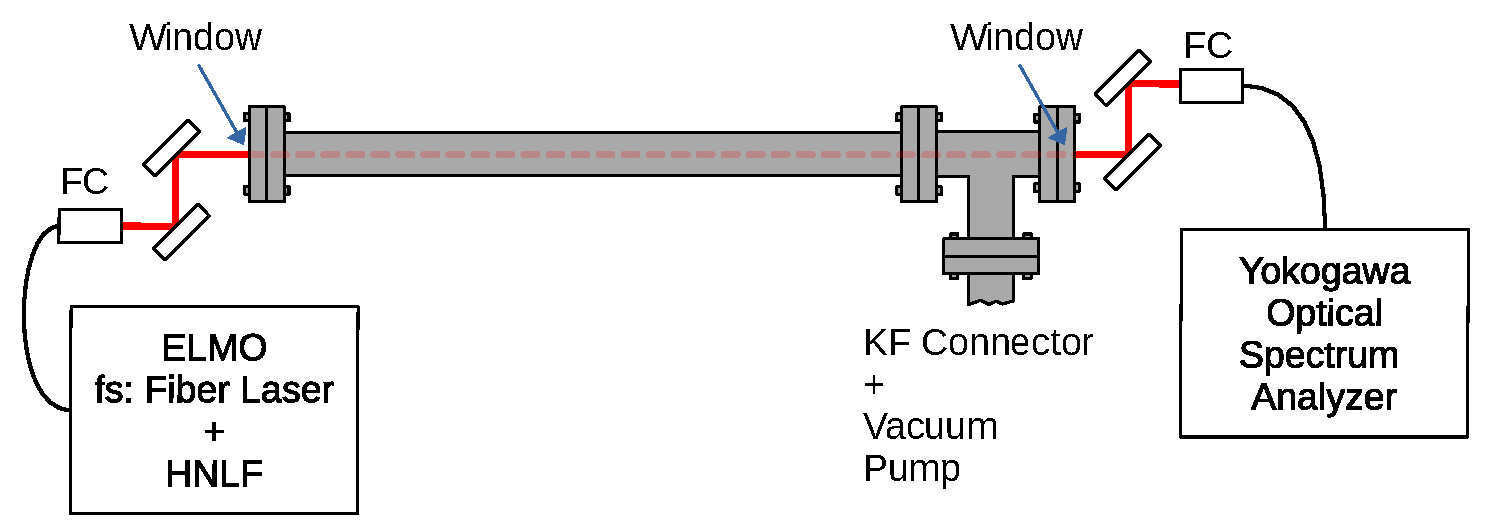
\includegraphics[width=0.95\linewidth]{diagrams/acetone_broadband_setup}
		\caption{Setup for single-pass direct absorption measurements of acetone vapor using a broadband fs-laser source. The measurement cell is able to be completely evacuated by the vacuum system so that a baseline can be measured using the same optical path. The spectrum of the fs-laser light is measured using a Yokogawa (AQ6375E) optical spectrum analyzer.}
		\label{fig:acetone_broadband_setup}
	\end{figure}
	
	
	\subsection{Results and Analysis}
	Overlayed in Fig. \ref{fig:acetone_broadband_rawdata} are each of the 10 measurements of the baseline and of the acetone absorption. These are plotted in logarithmic units (decibels), so absorption could be computed as the difference of the curves in this case.
	
	\begin{figure}[H]
		\centering
		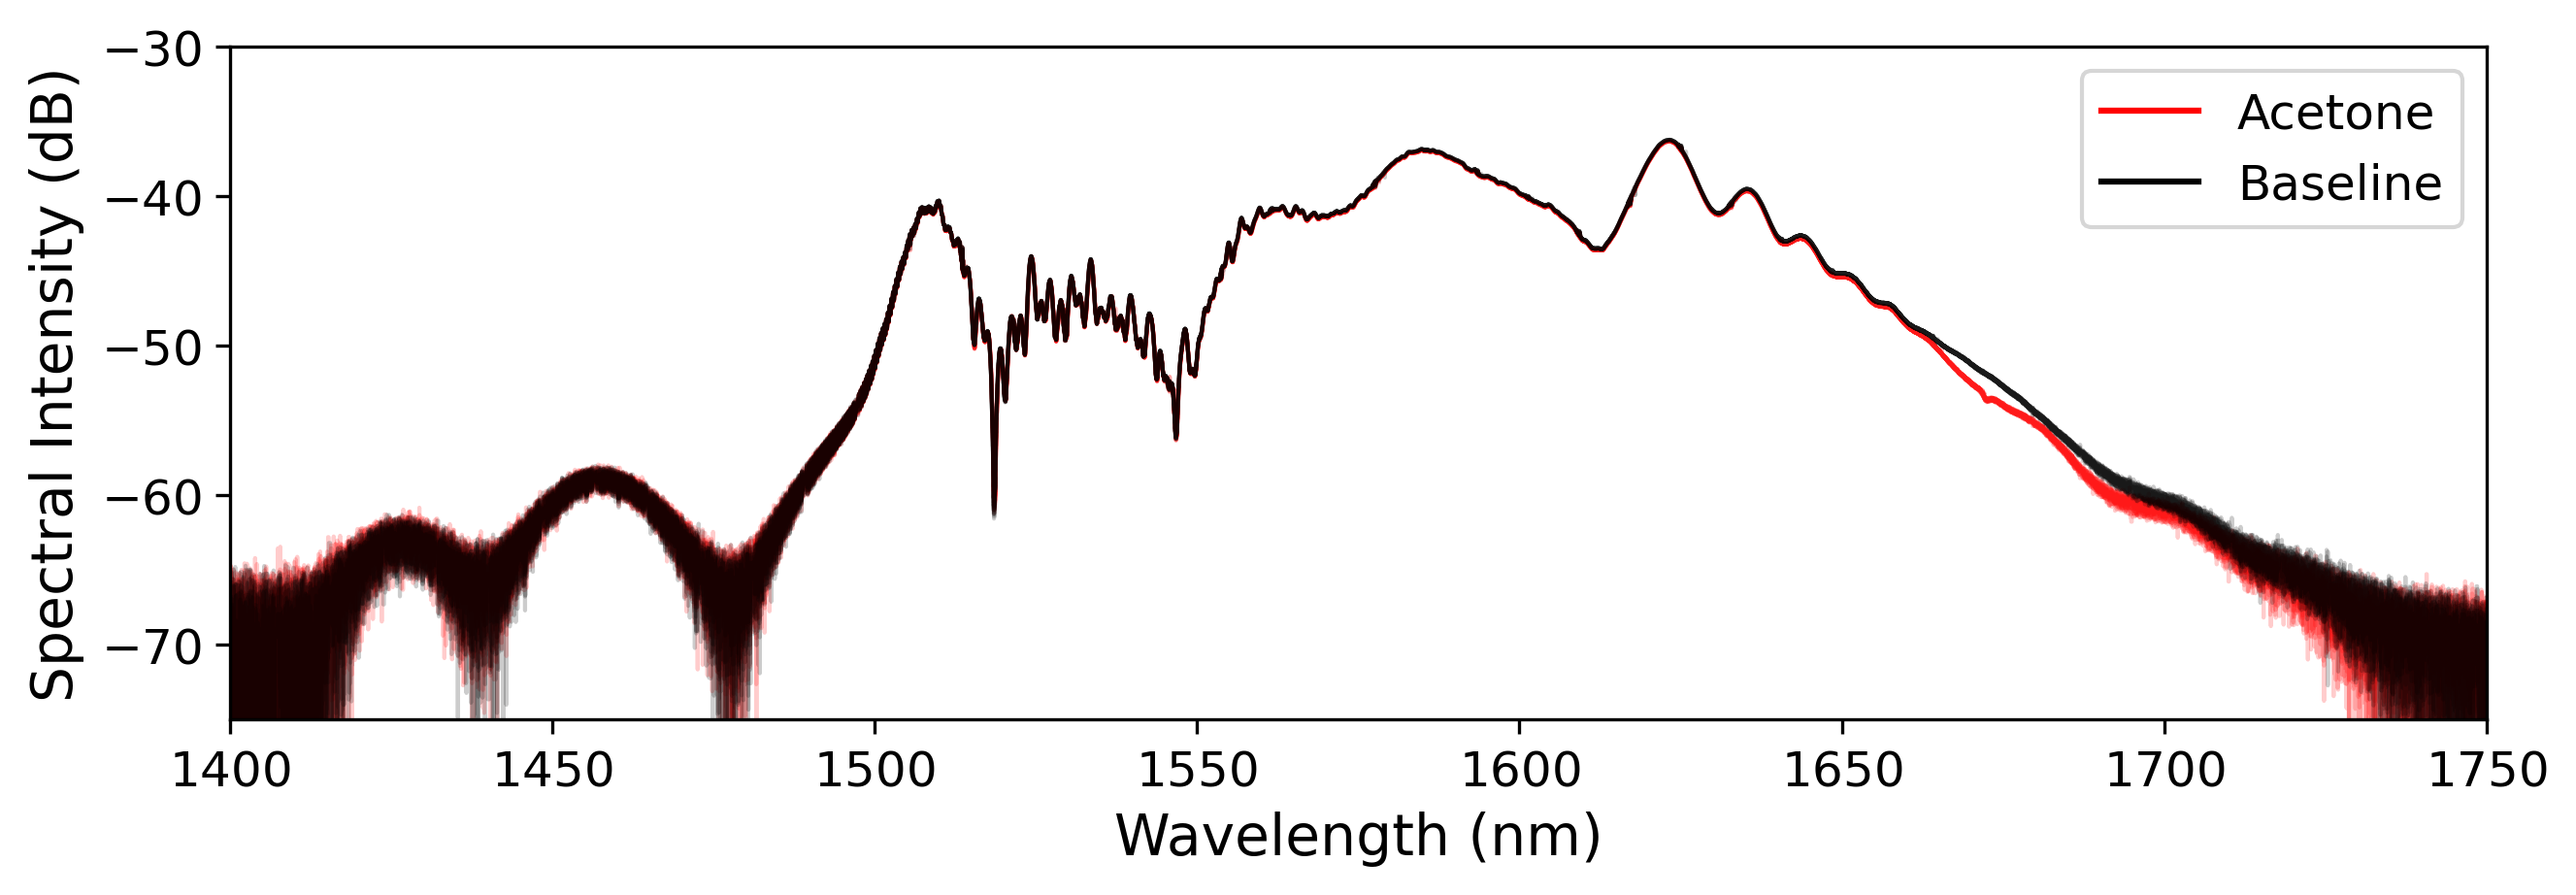
\includegraphics[width=1.0\linewidth]{diagrams/acetone_broadband_raw_data}
		\caption{Measurement of the NIR absorption coefficient of acetone. Two spectra are taken; one is taken with the measurement cell only filled with ambient air (the black baseline curve), and the other is taken with the cell filled with acetone (the red spectrum). An absorption coefficient is computed using \ref{beer-lambert-law}.}
		\label{fig:acetone_broadband_rawdata}
	\end{figure}
	
	Recalling from Ch. \ref{chap:fitting_spectra}, equation \ref{beer_absorp}, the absorption coefficient $\alpha(\lambda)$ for the wavelength $\lambda$ is given in terms of the baseline intensity $I_0(\lambda)$ and the absorbed intensity $I(\lambda)$ as
	\begin{equation}
		\alpha(\lambda) = \ln \left[I_0 / I\right]/L
	\end{equation}
	For each of the 10 baseline measurements an average was made, and the same was done for the acetone absorption measurements. The conversion to the absorption coefficient was performed on the averaged traces using the above relation. Shown in Fig. \ref{fig:acetone_broadband_results} is the absorption result after it has been converted into an optical cross section value.
	
	The conversion to the cross section value is performed by scaling the measured absorption by a constant value and applying a constant shift so that a least squares fit is performed to the model given by \ref{acetone_model}. This is easily done by the Appendix formulae (\ref{append_lsq_two_comp}) using the acetone model cross section $\sigma_\mathrm{ac}(\lambda)$ as a basis function to describe the measured absorption $\alpha(\lambda) = n \sigma_\mathrm{ac}(\lambda) + \alpha_0$. For each of the $i=1\ldots N$ wavelengths $\lambda_i$ falling within the range 1671.5-1675nm and the corresponding measured absorption value $\alpha_i$, we can evaluate the model acetone cross section $\sigma_i = \sigma_\mathrm{ac}(\lambda_i)$. This allows us to find the number density $n$ and the baseline correction $\alpha_0$ as
	\begin{align} \label{acetone_broadband_scaleFit}
		n = \frac{N \sum_i \alpha_i \sigma_i - \left(\sum_i \sigma_i\right)\left(\sum_i \alpha_i\right)}{N\sum_i\sigma_i^2 - \left(\sum_i\sigma_i\right)^2}  &&
		\alpha_0 = \frac{\left(\sum_i\sigma_i^2\right)\left(\sum_i\alpha_i\right) - \left(\sum_i\sigma_i\right)\left(\sum_i\alpha_i\sigma_i\right)}{N\sum_i\sigma_i^2 - \left(\sum_i\sigma_i\right)^2}
	\end{align}
	Once the number density and baseline correction are found from this range, the cross section is given over the whole measurement range by $\sigma(\lambda) = \left(\alpha(\lambda) - \alpha_0\right)/n$. The vertical scale of the data shown in Fig. \ref{fig:acetone_broadband_results} is the result of this process. The correctness of the baseline offset $\alpha_0$ obtained by the above relation can be seen by the fact that the cross section tends to zero in the region near 1600nm, indicating the successful extrapolation of our calibration.

	\begin{figure}[H]
		\centering
		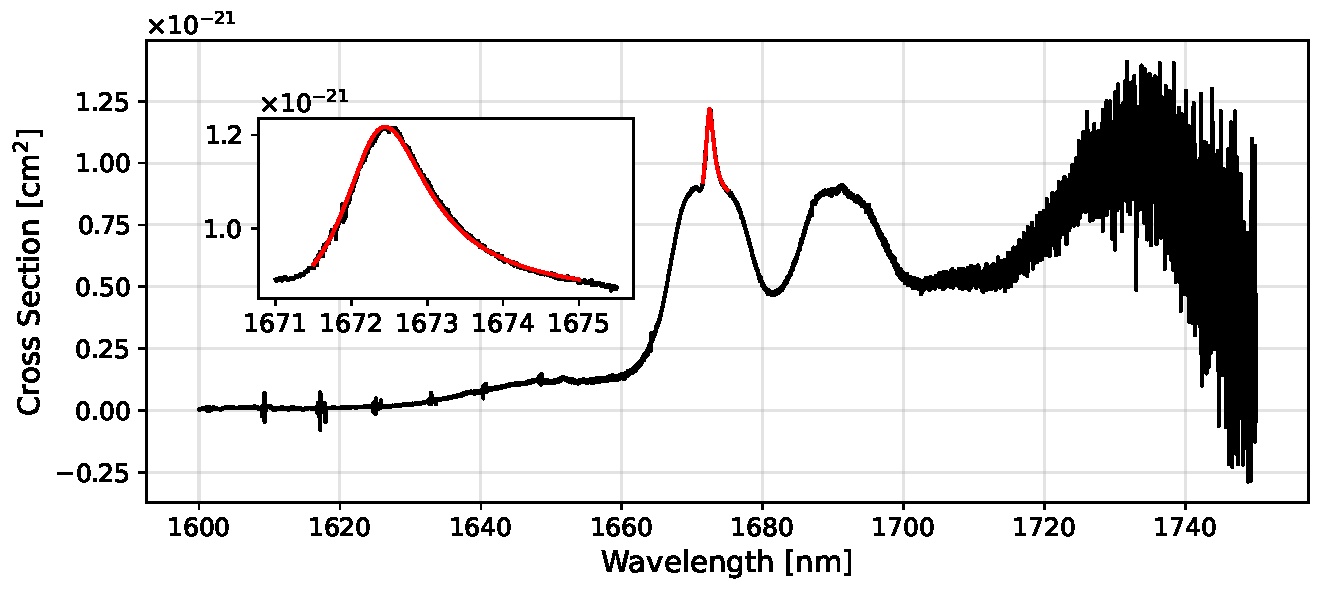
\includegraphics[width=1.0\linewidth]{diagrams/acetone_broadband_results}
		\caption{Shown in black is the measured NIR optical cross section for acetone, obtained from scaled absorption measurements. The scale was obtained by ensuring that the broadband measurement agrees with the model cross section (\ref{acetone_model}) presented in the previous section. This model cross section is shown with the red trace, where good agreement with the spectral shape of the broadband measurement can be seen. }
		\label{fig:acetone_broadband_results}
	\end{figure}
	
	\section{Expanded Cross Section Model}
	In this section, we construct a model of the NIR absorption cross section for acetone which is valid over a much larger range than the previous model given by \ref{acetone_model}. As before, this will be constructed from a fit to the absorption cross section data.
	
	In order to construct the most accurate model possible, we combine the cross section data obtained in Sec. \ref{sec:acetone_broadband} with the PNNL data presented in Fig. \ref{fig:acetone_PNNL_data}. Depicted in Fig. \ref{fig:acetone_broadband_stitch} is the construction of a dataset stitched together from our measurements and the PNNL data. The PNNL data was first scaled and offset to match our measurements using the same procedure as equation (\ref{acetone_broadband_scaleFit}). These measurements were themselves scaled and offset to match the narrowband acetone model of equation (\ref{acetone_model}). In effect, we are matching everything to the values given in Table \ref{table:acetone_coeffs}.
	
	Noting that the signal to noise ratio for our cross section data is better than the PNNL data for wavelengths shorter than 1685 nm (as can be seen in Fig. \ref{fig:acetone_broadband_stitch}a), we create a function to create a smooth transition between the two datasets. For this we define the crossover function of width $w_0$ and transition point $\lambda_0$ as
	\begin{equation}\label{acetone_crossover_func}
		c(\lambda) = \frac{1}{2} + \frac{1}{\pi}\tan^{-1}\left(\frac{\lambda - \lambda_0}{w_0}\right)
	\end{equation}
	The important feature of this function is that it monotonically transitions from 0 to 1 at the crossover point with a width controlled by $w_0$. Using this function, we create a new dataset $\sigma'_i$ from the PNNL data $\sigma^\mathrm{PNNL}_i$ and the measured data $\sigma^\mathrm{Meas}_i$ by the weighted sum
	\begin{equation}
		\sigma'_i =
		c(\lambda_i) \sigma^\mathrm{PNNL}_i + \Big(1-c(\lambda_i)\Big)\sigma^\mathrm{Meas}_i
	\end{equation}
	The stitched dataset, constructed using the above weighed sum, is shown in blue in Fig. \ref{fig:acetone_broadband_stitch}c).
	
	\begin{figure}[H]
		\centering
		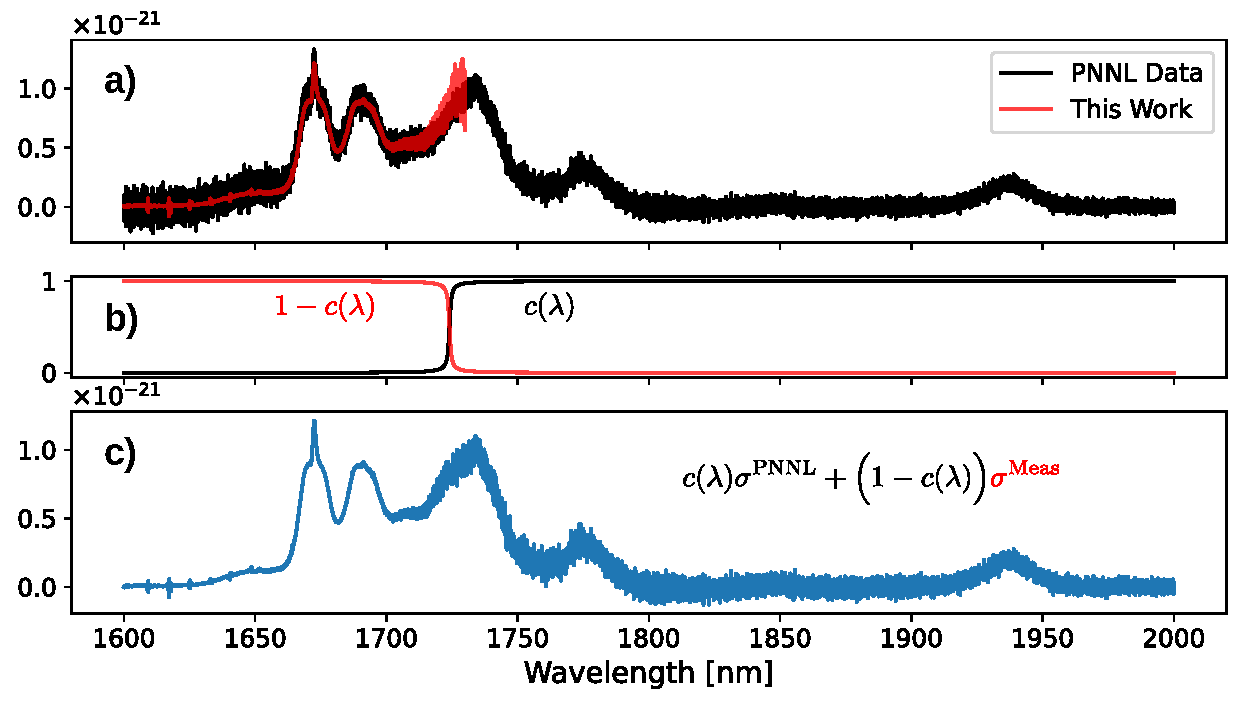
\includegraphics[width=1.0\linewidth]{diagrams/acetone_broadband_stitch}
		\caption{Process of stitching together our cross section measurements with those from the PNNL database \cite{pnnl_database_gas_phase, pnnl_isobutane}. The crossover function $c(\lambda)$ is given by Eq. (\ref{acetone_crossover_func}). The crossover point is chosen where the two datasets showed similar amounts of noise.}
		\label{fig:acetone_broadband_stitch}
	\end{figure}
	
	In order to provide an accessible empirical description of the acetone NIR absorption cross section, we construct the following fitting model consisting of a sum of Gaussian peaks and a modified version of the acetone peak from equation (\ref{sigma_tilde}). This model is given as
	\begin{equation} \label{acetone_super_model}
		\sigma_\mathrm{Acetone}(\lambda) = d_0 + d_1\frac{\Gamma_\mathrm{m}^2(\lambda-p_2)}{(\lambda-p_2)^2 + \Gamma_\mathrm{m}^2(\lambda-p_2)} + \sum_{i=0}^{11} c_{i0} \exp \left[-(x-c_{i1})^2/c_{i2}^2\right]
	\end{equation}
	The function $\Gamma_\mathrm{m}(\lambda)$ is modified from the earlier definition (\ref{Lambda}) to allow the model of the peak to tend to zero for wavelengths far away from the peak. That is, we now satisfy $\lim\limits_{\lambda\rightarrow\pm\infty}\sigma_\mathrm{Acetone}(\lambda) = 0$.  We arbitrarily chose the arctangent function to clamp the $\Gamma(\lambda)$ function away from the peak leading to the modified function
	\begin{equation}
		\Gamma_\mathrm{m}(\lambda) = p_0 + p_1 p_3 \tan^{-1}\left(\frac{\lambda}{p_3}\right)
	\end{equation}
	The important feature of this function is that it behaves linearly around $\lambda \sim 0$, but far away from this center, the function approaches a constant value (it is clamped). The width of the transition is controlled by $p_3$, a new fitting parameter.
	
	The values of $p_{0,2}$ are taken from Table \ref{table:acetone_coeffs}, enabling the use of high-resolution peak shape information from the CRDS data presented in Sec. \ref{sec:acetone_peak}. The value of $p_1$ is treated as a free fit parameter to account for the modified the baseline on which the acetone peak function, $\tilde{\sigma}_{\mathrm{ac}}(\lambda)$ given by (\ref{sigma_tilde}), is situated.
	
	A nonlinear least-squares routine was employed to fit the coefficients $c_{i,j}$, $d_{0,1}$, and $p_{1,3}$ to the stitched dataset by minimizing the sum of squared residuals. Initial parameters for the acetone peak were derived from our previous work, while the coefficients corresponding to the twelve Gaussian peaks for the baseline were initialized through visual inspection of the data. These values were then iteratively optimized until an optimal fit was converged upon. The result of this fit is plotted in Fig. \ref{fig:acetone_broadband_superfit}.
	
	In the inset of Fig. \ref{fig:acetone_broadband_superfit}, we can see in detail the peak which was earlier investigated. The blue trace is the result of plotting the fit curve with $d_1=0$, where we can see the Gaussian baseline, on top of which the peak sits. The nonlinearity of this feature necessitates the modification of the $p_1$ coefficient.
	
	\begin{figure}[H]
		\centering
		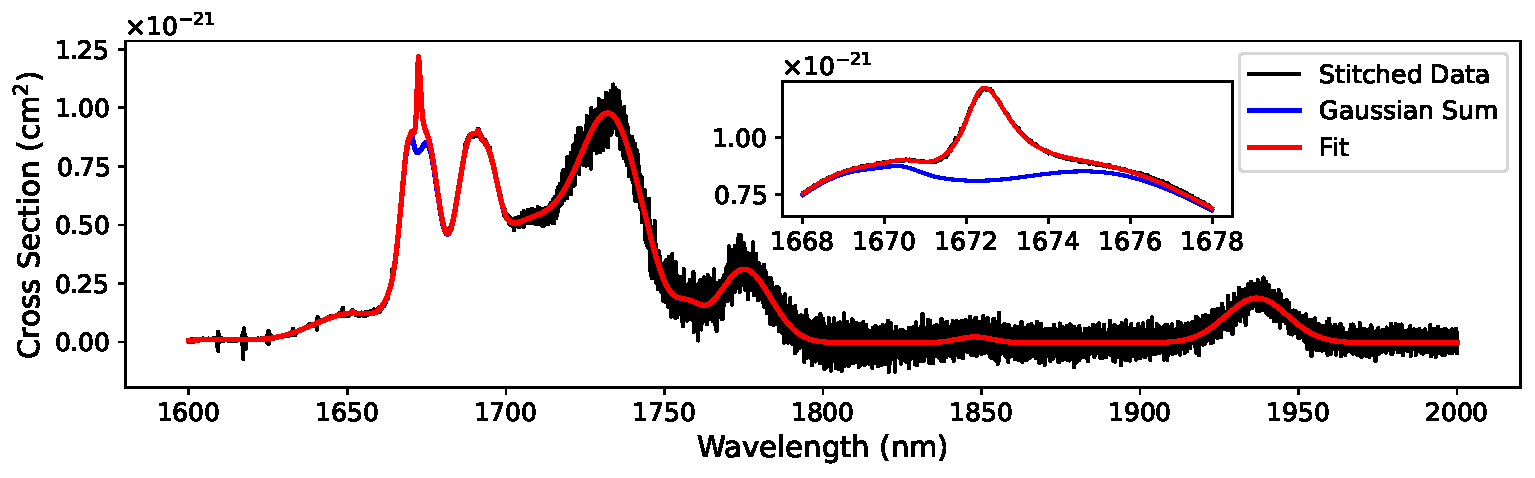
\includegraphics[width=1.0\linewidth]{diagrams/acetone_broadband_superfit}
		\caption{Fit of the extended range acetone absorption cross section model (\ref{acetone_super_model}) to the stitched together data which was constructed from our measurements and PNNL data \cite{pnnl_database_gas_phase, pnnl_isobutane}. The inset shows the fit near the peak feature which was investigated in Sec. \ref{sec:acetone_peak}. The values for the fit are shown in Table \ref{tbl:acetone_broadband_coeffs}. The values for $p_{0}$ and $p_2$ were taken from Table \ref{table:acetone_coeffs}, preserving the precise wavelength value of the peak, as well as some of the high-resolution shape information obtained in Sec. \ref{sec:acetone_peak}. The computer code for plotting the fitted function shown in red is given in \ref{sec:subsys_acetone_function}.}
		\label{fig:acetone_broadband_superfit}
	\end{figure}
	
	\begin{table}[H]
		\caption{Coefficients which allow the re-construction of the acetone cross section fit curve shown in Fig. \ref{fig:acetone_broadband_superfit} using equation (\ref{acetone_super_model}). These are found from a nonlinear fit to the data which is stitched together from both our measurements and those in the PNNL database. The left table corresponds by column to the amplitudes, centers, and widths of the Gaussian functions used to fit the acetone cross section. The right table gives the coefficients for the  Note that the values of $p_0$ and $p_2$ are taken from Table \ref{table:acetone_coeffs}.}
		\begin{center}
			\begin{tabular}{|c|c|c|}
				\hline
				$c_{i0}$ [cm$^2$] & $c_{i1}$ [nm] & $c_{i2}$ [nm] \\
				\hline
				$1.36 \times 10^{-23}$ & $1608.26$ & $17.04$ \\
				\hline
				$1.2 \times 10^{-22}$ & $1650.89$ & $17.33$ \\
				\hline
				$7.75 \times 10^{-24}$ & $1651.73$ & $0.42$ \\
				\hline
				$3.84 \times 10^{-22}$ & $1668.98$ & $2.89$ \\
				\hline
				$2.18 \times 10^{-22}$ & $1667.76$ & $5.42$ \\
				\hline
				$2.32 \times 10^{-23}$ & $1670.45$ & $0.52$ \\
				\hline
				$6.77 \times 10^{-22}$ & $1675.20$ & $5.02$ \\
				\hline
				$5.41 \times 10^{-22}$ & $1688.29$ & $5.47$ \\
				\hline
				$2.39 \times 10^{-23}$ & $1691.33$ & $0.54$ \\
				\hline
				$2.72 \times 10^{-22}$ & $1694.94$ & $4.10$ \\
				\hline
				$5.1 \times 10^{-22}$ & $1706.87$ & $26.33$ \\
				\hline
				$7.92 \times 10^{-22}$ & $1733.92$ & $13.99$ \\
				\hline
				$9.21 \times 10^{-23}$ & $1757.64$ & $5.58$ \\
				\hline
				$3.13 \times 10^{-22}$ & $1775.23$ & $11.86$ \\
				\hline
				$2.53 \times 10^{-23}$ & $1847.86$ & $7.63$ \\
				\hline
				$1.91 \times 10^{-22}$ & $1936.87$ & $13.74$ \\
				\hline
			\end{tabular}
			\begin{tabular}{|c|c|c|c|}
				\hline
				$d_{1}$ [cm$^2$] & $d_{0}$ [cm$^2$] & $p_1$ & $p_3$ [nm] \\
				\hline
				$4.08 \times 10^{-22}$ & $-3.62 \times 10^{-24}$ & $0.330$ & $0.340$ \\
				\hline
			\end{tabular}
		\end{center}
		\label{tbl:acetone_broadband_coeffs}
	\end{table}
	
	To the best of our knowledge, model (\ref{acetone_super_model}) and the values presented in the above table represent the most accurate spectroscopic reference for the acetone absorption cross-section within the 1600–1685 nm range currently available in the literature. Concise computer code for the evaluation the acetone NIR cross section described by function (\ref{acetone_super_model}) is given in \ref{sec:subsys_acetone_function}.
	
	\section{Followup Investigation of Acetone Concentration Drift} \label{sec:acetone_broadband_drift}
	The observation of a slow temporal drift of the observed spectrum of gaseous acetone stored in a sealed metal vessel was reported in our previous work \cite{mine_acetone}, which is also described in Sec. \ref{sec:acetone_drift}. In this section we report additional observations of this effect.
	
	In Fig. \ref{fig:acetone_drift_longtermheating}, the rise of the acetone number density is seen clearly over the span of many days. Halfway through the data collection, a heater was applied to the aluminum chamber walls. The temperature was only changed slightly, by approximately 10-15$^\circ$C in regions where the heat was applied, and this was not consistent over the whole chamber. The rise in the production of acetone vapor is evidence that there is a kind of transport limited reservoir of acetone stuck in the measurement chamber. This could be attributed to the porous metal surface trapping hidden reservoirs of acetone. The observation of the temperature dependence of this evolution gives evidence in favor of a diffusion-limited transport.
	
	\begin{figure}[H]
		\centering
		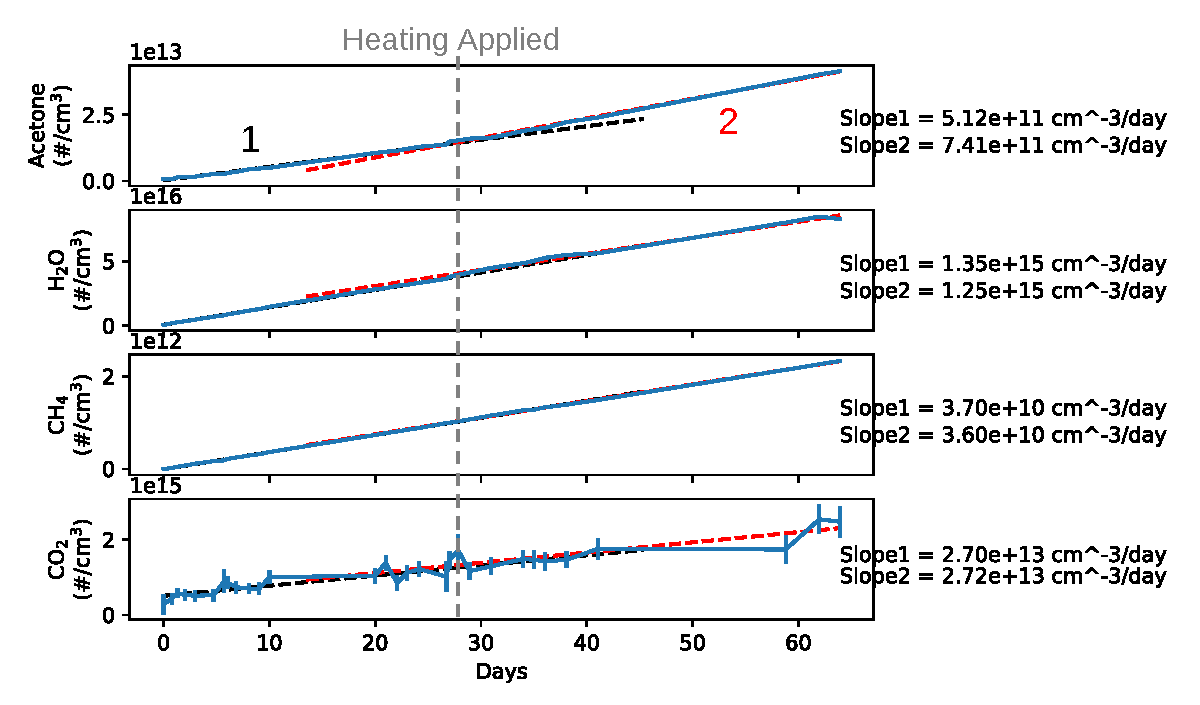
\includegraphics[width=1.0\linewidth]{diagrams/acetone_drift_longterm_heating}
		\caption{Number density of acetone, water, methane, and carbon dioxide obtained from CRDS spectrum fits of a sample contained in a closed aluminum chamber with a very slow leak. The appearance of acetone vapor in concentrations much greater than ambient air hints at long-term contamination of the metal chamber walls with residual acetone. The vertical line which appears approximately half-way through the measurement marks the beginning of external heating of the chamber walls. It is clear that the rate of acetone appearance increases with the supplied heating, indicating a diffusion limited surface effect.}
		\label{fig:acetone_drift_longtermheating}
	\end{figure}
	
	Another transient dependence of the acetone spectrum was observed during the measurement of the broadband absorption spectrum. When the measurement cell was first filled, a large broadband absorption was observed. Over several minutes this large absorption settled down into the shape reported in Fig. \ref{fig:acetone_broadband_results}. This transient behavior is shown in Fig. \ref{fig:acetone_broadband_drift}, where the absorption is plotted every 28 seconds. The filling procedure of the cell may be partially responsible for this behavior. In this case, the acetone was introduced into the measurement cell by liquid drops which were then allowed to evaporate. Some of the behavior displayed in Fig. \ref{fig:acetone_broadband_drift} may be partially due to the formation of droplets which can scatter the laser light, producing a loss indistinguishable from absorption. It should be noticed that the time scale of these variations is consistent with the fast settling behavior observed with calibration gas samples in Fig. \ref{fig:actetone_crds_drifts}.
	
	\begin{figure}[H]
		\centering
		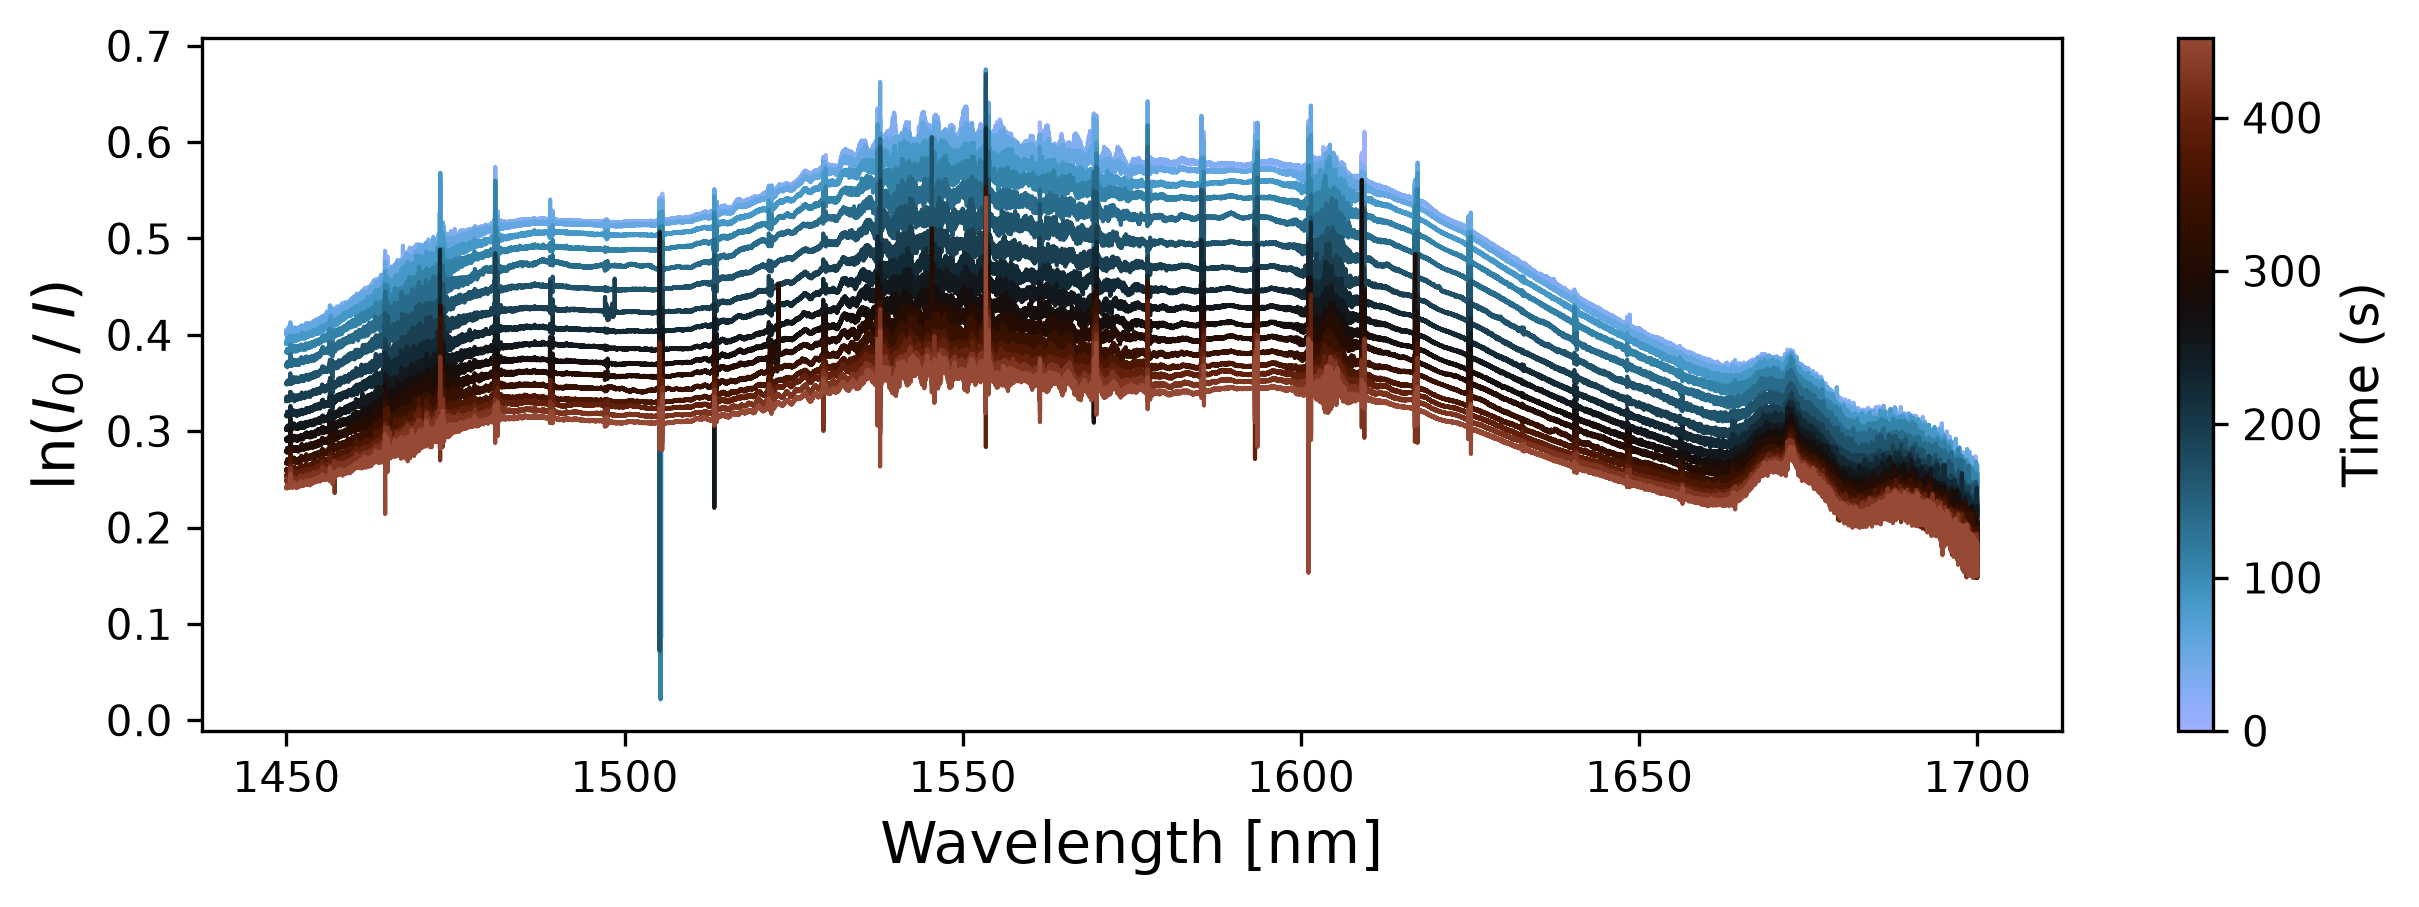
\includegraphics[width=1.0\linewidth]{diagrams/acetone_broadband_drift}
		\caption{Time sequence of optical depth $\alpha L$ measurements, taken every 28 seconds, of a closed metal vessel containing evaporating acetone liquid. It can be seen that a much more broadband transient absorption is observed when the acetone is initially placed in the vessel. After a long period of time, the spectrum settles into the shape shown in previous measurements. On the long-wavelength side of the plot, the appearance of the equilibrium absorption shape can be seen.}
		\label{fig:acetone_broadband_drift}
	\end{figure}
	
	\section{Summary and Conclusions}
	At the onset of this work, few spectroscopic references were available for the NIR absorption cross-section of acetone, a critical analyte for breath diagnostics. The development of an optical breath diagnostic platform based on NIR absorption depends heavily on the availability of accurate spectroscopic references; without them, it is impossible to derive precise gas concentration information from an optical absorption spectrum.
	
	In the beginning of this chapter we showed some plots of the current "state of the art" spectroscopic references for acetone (see Fig. \ref{fig:acetone_PNNL_data}). Without additional processing, the excess noise in the NIR portion of these measurements limits much of their utility when performing fits to spectroscopic absorption data. To address this deficiency, we present empirical models which can be evaluated as smooth curves without the introduction of this measurement noise.
	
	In great detail we examined the distinctive peak centered near a wavelength of 1672.4 nm, resulting in the narrowband empirical model (\ref{acetone_model}) for the acetone cross section along with the coefficients given in Table \ref{table:acetone_coeffs}. Even in this small wavelength range, we demonstrated that this spectral region was already useful for multi-species breath characterization.
	
	The absorption cross-section magnitude was determined using the narrowband empirical model as a calibration standard for the broadband acetone measurements. Within a specific region of the NIR spectrum, encompassing the 1672.4 nm peak, our measurements exhibited lower noise levels than those found in the PNNL database. By combining our high-precision data with the broadband PNNL dataset, we achieved a global fit that constitutes an improved model for the broadband acetone absorption cross-section. The high-resolution shape information of the previously identified peak was preserved through the strategic selection of free fitting parameters.
	
	
	\chapter{A PROCEDURE FOR SIMULTANEOUS EVALUATION OF GAS CONCENTRATIONS AND LASER TUNING BEHAVIOR} \label{chap:det}
	The extraction of precise gas concentrations from absorption spectra is fundamentally constrained by the accuracy of the wavelength axis. In traditional spectroscopic analysis, the wavelength of each data point is assumed to be known via external calibration, such as a continuous wavemeter measurement. However, the utility of this approach is limited by the precision and stability of the calibration hardware; any uncertainty in $\lambda$ propagates through the spectral model, introducing systematic errors into the concentration estimates. This effect is most pronounced near regions of high absorption gradients ($\partial\alpha/\partial\lambda$), where even minute wavelength offsets can manifest as significant distortions in the reconstructed absorption profiles. Achieving the precision required for complex, overlapping spectral features often necessitates calibration instrumentation with a footprint and complexity that rival the primary CRDS instrument itself.
	
	In this chapter, we propose an alternative approach: rather than treating wavelength as an externally measured independent variable, we treat it as a set of coupled parameters within a global optimization problem. We demonstrate that if the laser wavelength can be modeled as a deterministic function of controllable experimental parameters--specifically the injection current ($I$) and the temperature ($T$) of the DFB diode laser--then the wavelength axis can be reconstructed from the history of these control signals.
	
	\section{Extraction of Laser Detuning as an Optimization Problem}
	If the experimental scanning conditions are sufficiently controlled such that the laser wavelength can be described by a deterministic detuning function, $\lambda(I, T)$, then the reconstruction of this function during post-processing effectively recovers the wavelength for every data point in the spectrum. Provided that these reconstructed values coincide with high precision with the true laser wavelengths, the gas concentrations can be extracted with a level of sensitivity and precision competitive with traditional, externally calibrated methods.
	
	We can motivate such a procedure by first envisioning that we already know the set of coefficients $\mathbf{a}$ which define the detuning function $\lambda(I, T;\;\mathbf{a})$. When we conduct the scan of the laser wavelength, we record the temperatures $T_i$ and currents $I_i$ of each scan point. Knowledge of the detuning coefficients allows us to compute the wavelength $\lambda_i = \lambda(T, I;\; \mathbf{a})$ of each scan point, and we can therefore evaluate the optical cross section $\sigma_j(\lambda_i)$ of the $j^\mathrm{th}$ species we intend to characterize. With this knowledge we can compute the concentrations of the relevant species using (\ref{leastSquares}). These obtained concentrations could then be used to compute a curve of best fit. By computing the error between this curve of best fit and the measured absorption values, we can obtain a single scalar value which is minimized when the detuning coefficients $\mathbf{a}$ are chosen accurately. The procedure of finding these detuning coefficients is performed by minimizing this scalar error value through a nonlinear optimization procedure.
	
	By minimizing a joint error function that accounts for both the species concentrations and the tuning coefficients, we drive the system toward a state where the predicted absorption profiles (derived from established databases such as HITRAN) are in optimal alignment with the observed spectral features. This approach effectively transforms wavelength uncertainty from an uncorrected source of systematic spectral distortion into a solvable parameter estimation problem, provided the laser tuning behavior remains reproducible within a single scanning direction.
	
	The primary obstacle to this approach is the inherent presence of hysteresis in continuous-wave (CW) laser tuning. Variations in environmental conditions or the historical state of the laser parameters can result in the same set of injection currents ($I$) and temperatures ($T$) yielding disparate emission wavelengths. To ensure the validity of a single-valued model, experimental protocols must be implemented to minimize these hysteretic effects. In this work, we achieved this by maintaining a stable thermal environment for the laser source and ensuring that the tuning procedure was performed with strict adherence to a consistent scanning protocol.
	
	Specifically, hysteresis in the DFB lasers utilized in this study was minimized by maintaining a unidirectional scanning trajectory. By adopting a protocol of decreasing temperature and decreasing current, we ensured that for any given set of $(I, T)$ parameters, the wavelength $\lambda$ is described by a single-valued function, provided the parameters are approached from a consistent direction in the parameter space. This reduction of the tuning behavior to a deterministic mapping allows the optimization algorithm to converge on a stable solution for the detuning coefficients.
	
	\section{Optimization Parameter Definition}
	The optimization problem presented here can be formulated by defining an objective function, $F$, which represents the weighted residual between the experimental absorption and the theoretical model. Let the set of $m$ coefficients $\mathbf{a} = \{a_0, a_1, \dots, a_{m-1}\}$ define the detuning function $\lambda(I, T; \mathbf{a})$. The error function is then defined as:
	
	\begin{equation}
		F(\mathbf{a}) = \sum_{i=1}^{N} \Big[ \alpha_\mathrm{model}(\lambda_i) - \alpha(\tau_i, \tau_0(\lambda_i)) \Big]^2 w^2(\tau_i)
	\end{equation}
	
	where $\lambda_i = \lambda(I_i, T_i;\,\mathbf{a})$ is the wavelength reconstructed from the measured control parameters at each data point. 
	
	A significant computational challenge in such a multi-parameter estimation problem is the high dimensionality of the search space, particularly when considering both the tuning coefficients $\mathbf{a}$ and the concentrations of multiple gas species, $\{c_j\}$. To mitigate this, we implement a nested optimization strategy that significantly reduces the complexity of the parameter space. 
	
	At each iteration of the nonlinear optimizer (e.g., the Nelder-Mead algorithm), the current estimate of the coefficients $\mathbf{a}$ is used to reconstruct the wavelength axis $\lambda_i$. Once this axis is established, the concentrations $c_j$ are not treated as independent nonlinear variables; rather, they are determined analytically via the linear least-squares decomposition described in Equation (\ref{leastSquares}). Because the concentration retrieval is non-iterative and depends only on the current reconstructed wavelength, the optimization manifold is reduced strictly to the $m$ dimensions of the tuning coefficients. This decoupling ensures that the optimizer does not need to navigate the high-dimensional concentration space, allowing for rapid convergence while simultaneously optimizing the spectral alignment and the concentration estimates.
	
	\subsection{Choice of the Nonlinear Optimizer}
	The choice of optimization algorithm is constrained by the topology of the error surface $F(\mathbf{a})$. Because many of the identifying absorption features in our spectra are highly localized in wavelength space, the objective function is characterized by a "needle-in-a-haystack" landscape: the error remains relatively constant and featureless across large regions of the parameter space, only exhibiting significant changes when the reconstructed wavelengths $\lambda_i$ bring the predicted cross-sections into alignment with the observed absorption peaks. For gradient-based optimizers, such as Levenberg-Marquardt or steepest descent, this landscape presents a profound challenge; in the wide, flat regions of the cost function where the derivatives $\partial F/\partial a_i$ are vanishingly small, the optimizer lacks the directional information necessary to navigate toward the local minimum.
	
	To circumvent the issues associated with gradient estimation, we employ the Nelder-Mead simplex algorithm. As a derivative-free method, Nelder-Mead relies on the evaluation of the function at the vertices of a moving simplex, allowing it to "crawl" across the flat regions of the error surface by probing the relative values of $F$ rather than relying on local slopes. 
	
	However, the efficacy of this approach is heavily dependent on the quality of the initial guess for the coefficients $\mathbf{a}$. If the initial wavelength reconstruction is too far from the true tuning behavior, the optimizer may become trapped in a sub-optimal local minimum or fail to find the feature entirely.
	
	\section{Characterization of the Laser Detuning Function}
	
	The success of the simultaneous optimization procedure described previously relies on the existence of a deterministic mapping between the laser's control parameters--injection current ($I$) and temperature ($T$)--and the resulting emission wavelength ($\lambda$).
	
	The emission wavelength of the diode laser must be an allowed mode of the internal optical cavity, and the spacing of these modes is determined by the temperature dependent refractive index of the medium \cite{book_pankove1971}. This mode spacing, along with the effective round-trip gain of the lasing medium, determine the ultimate emission wavelength \cite{book_lasers_siegman}. While the laser output may actually be a combination of several lasing wavelengths, the devices are generally constructed to favor just one of these modes for a range of operating temperatures and currents. 
	
	For the purposes of our optimization framework, we require a mathematical model that can represent this tuning behavior with sufficient precision to match the narrow linewidths of molecular absorption features. We approach this by constructing a hierarchy of models: beginning with a first-order planar approximation for initial parameter estimation, and progressing to a higher-order Taylor expansion for high-precision reconstruction.
	
	In this work, we characterize the tuning behavior of four DFB diode lasers (Table \ref{table:diodes}). The manufacturer specifications sometimes provide an initial linear approximation of the tuning sensitivity, suggesting that the wavelength can be roughly modeled by a planar function of $I$ and $T$
	\begin{equation} \label{det_plane_P3}
		\lambda_{\mathrm{P3}}(I, T;\;\mathbf{a}) = a_0 + a_1 I + a_2 T
	\end{equation}
	In our optimization loop, these manufacturer-provided coefficients serve as the critical "initial guess" for the $a_i$ parameters. While this planar model is computationally efficient, experimental measurements in our laboratory demonstrate that it is insufficient to capture the full complexity of the tuning manifold. As shown in Fig. \ref{fig:det_detuningsurface}, the true wavelength evolution exhibits systematic deviations from this linear model that are significant relative to the precision required for trace gas spectroscopy.
	
	To bridge the gap between this first-order approximation and the experimental reality, we employ a more robust quadratic expansion in the following section. This allows us to capture the second-order dependencies--such as the interplay between thermal and current-induced shifts--required to achieve the high-fidelity wavelength reconstruction necessary for our simultaneous fitting procedure.
	
	\subsection{Laser Devices}
	
	In this work, we will investigate the behavior of four DFB diode lasers. The manufacturer specifications are shown in Table \ref{table:diodes}, along with the equivalent parameters measured in our lab. The tuning coefficients specified by the manufacturer imply that a linear model can be used in both temperature and current parameters. We have directly measured the tuning profiles of the lasers and these are plotted alongside a planar fit model. 
	
	We have additionally plotted the deviation from this fit, which shows clear systematic difference from the planar model.
	
	\begin{table}[H] 
		\begin{center}
			\caption{DFB laser diodes investigated in this work. The measured tuning is obtained from the coefficients of the planar fit to the tuning behavior shown in Fig \ref{fig:det_detuningsurface}.}\label{table:diodes}
			\begin{tabular}{|c|c|c|c|c|c|c|c|}
				\hline
				No. & Manufacturer & Lower & Upper  & Meas. Tuning & Meas. Tuning \\
				& & Range & Range & (nm/mA) & (nm/$^\circ$C) \\
				\hline
				1 & Eblana & 1651.4 nm & 1655.2 nm & 2.04$\times10^{-2}$ & 9.95$\times10^{-2}$ \\
				 & EP1653-7-DM-B01-FM & & & &  \\
				\hline
				2 & Eblana & 1657.7 nm & 1662.0 nm & 2.57$\times10^{-2}$ & 1.12$\times10^{-1}$ \\
				& EP1659-0-DM-B01-FM & & & &  \\
				\hline
				3 & Eblana & 1671.6 nm & 1675.6 nm & 2.03$\times10^{-2}$ & 1.05$\times10^{-1}$ \\
				& EP1673-7-DM-B01-FM & & & &  \\
				%\hline
				%4 & NEL & - & - & - & - & -\\
				\hline
			\end{tabular}
		\end{center}
	\end{table}
	
	
	Typical wavelength tuning sensitivities for diodes operating near 1650nm are on the order of 0.02 nm/mA for current changes, and 0.1 nm/$^\circ$C for temperature changes \cite{crds_co2_scanning_noaom}.
	
	The diodes investigated in this work were all of the fiber pigtailed 14 butterfly package, which feature an on-board Peltier element to directly cool the laser diode and a thermistor-type temperature transducer to enable a feedback control loop by a controller. The temperature and current were stabilized by a (previously ILX Lightwave-) Newport LDC-3900 laser diode controller equipped with LCM-39420 current source and temperature controller module.
	
	\section{The Static Tuning Profile}
	In this section, we provide a mathematical description for the detuning function $\lambda(I,T)$. This is done by first taking measurements of the tuning profile for three DFB lasers and using progressively more sophisticated models to describe the behavior. The tuning profiles measured for this can be considered as steady state in the sense that the laser has had sufficient time to equilibrate to its new wavelength each time a change to the control parameters $I$ and $T$ is made.
	
	\subsection{The Q6 Quadratic Tuning Model}
	The core assumption of this method is that the laser detuning can be described by a single valued function $\lambda(I, T)$. If this function is smoothly varying as the input parameters are changed, then this function can be expressed as the Taylor series expansion around some operating point of the temperature $T_0$ and current $I_0$
	\begin{align} \label{det_taylor}
		\lambda (I, T) &\approx \lambda(I_0, T_0) + (I-I_0) \frac{\partial \lambda}{\partial I} \Bigg|_{T_0,I_0} + (T-T_0)\frac{\partial \lambda}{\partial T}\Bigg|_{T_0,I_0}
		\nonumber\\&\;\;\;\;\;\; + \frac{1}{2} (T-T_0)^2 \frac{\partial^2 \lambda}{\partial T ^2}\Bigg|_{T_0,I_0}  + \frac{1}{2}(I-I_0)^2\frac{\partial^2 \lambda}{\partial I ^2}\Bigg|_{T_0,I_0} + (T-T_0)(I-I_0)\frac{\partial \lambda}{\partial I} \frac{\partial \lambda}{\partial T}\Bigg|_{T_0,I_0} 
	\end{align}
	Expanding this expression leads to the quadratic form
	\begin{equation} \label{det_quadratic}
		\lambda_\mathrm{Q6}(I, T;\; \vec{\mathbf{a}}) = a_0 + a_1 I + a_2 T + a_3 I^2 + a_4 T^2 + a_5 IT
	\end{equation}
	
	This $Q6$ model extends the planar approximation by incorporating the curvature and cross-coupling terms (the $I^2, T^2,$ and $IT$ components) necessary to describe the non-linearities observed in DFB diode tuning.
	
	The performance of this model in representing the experimental tuning profiles is illustrated in Fig. \ref{fig:det_detuningsurface}. The figure presents a three-stage decomposition of the tuning data: (a) the raw wavelength measurements, (b) the residuals remaining after subtracting the first-order planar fit, and (c) the residuals following the application of the $Q6$ model. As shown in the rightmost panels, the $Q6$ model reduces the systematic deviation to within $\sim 2$ parts in $10^6$.
	
	While higher-order systematic deviations persist--as evidenced by the non-zero residuals in the $Q6$ plots--the magnitude of these errors remains several orders of magnitude smaller than the Full Width at Half Maximum (FWHM) of the molecular absorption features under investigation. Consequently, for the purposes of spectral reconstruction, the $Q6$ model provides a sufficiently accurate description of the wavelength axis, and further increasing the complexity of $\lambda(I, T)$ would introduce unnecessary degrees of freedom into the global optimization without yielding a significant improvement in concentration accuracy.
	
	\begin{figure}[H]
		\centering
		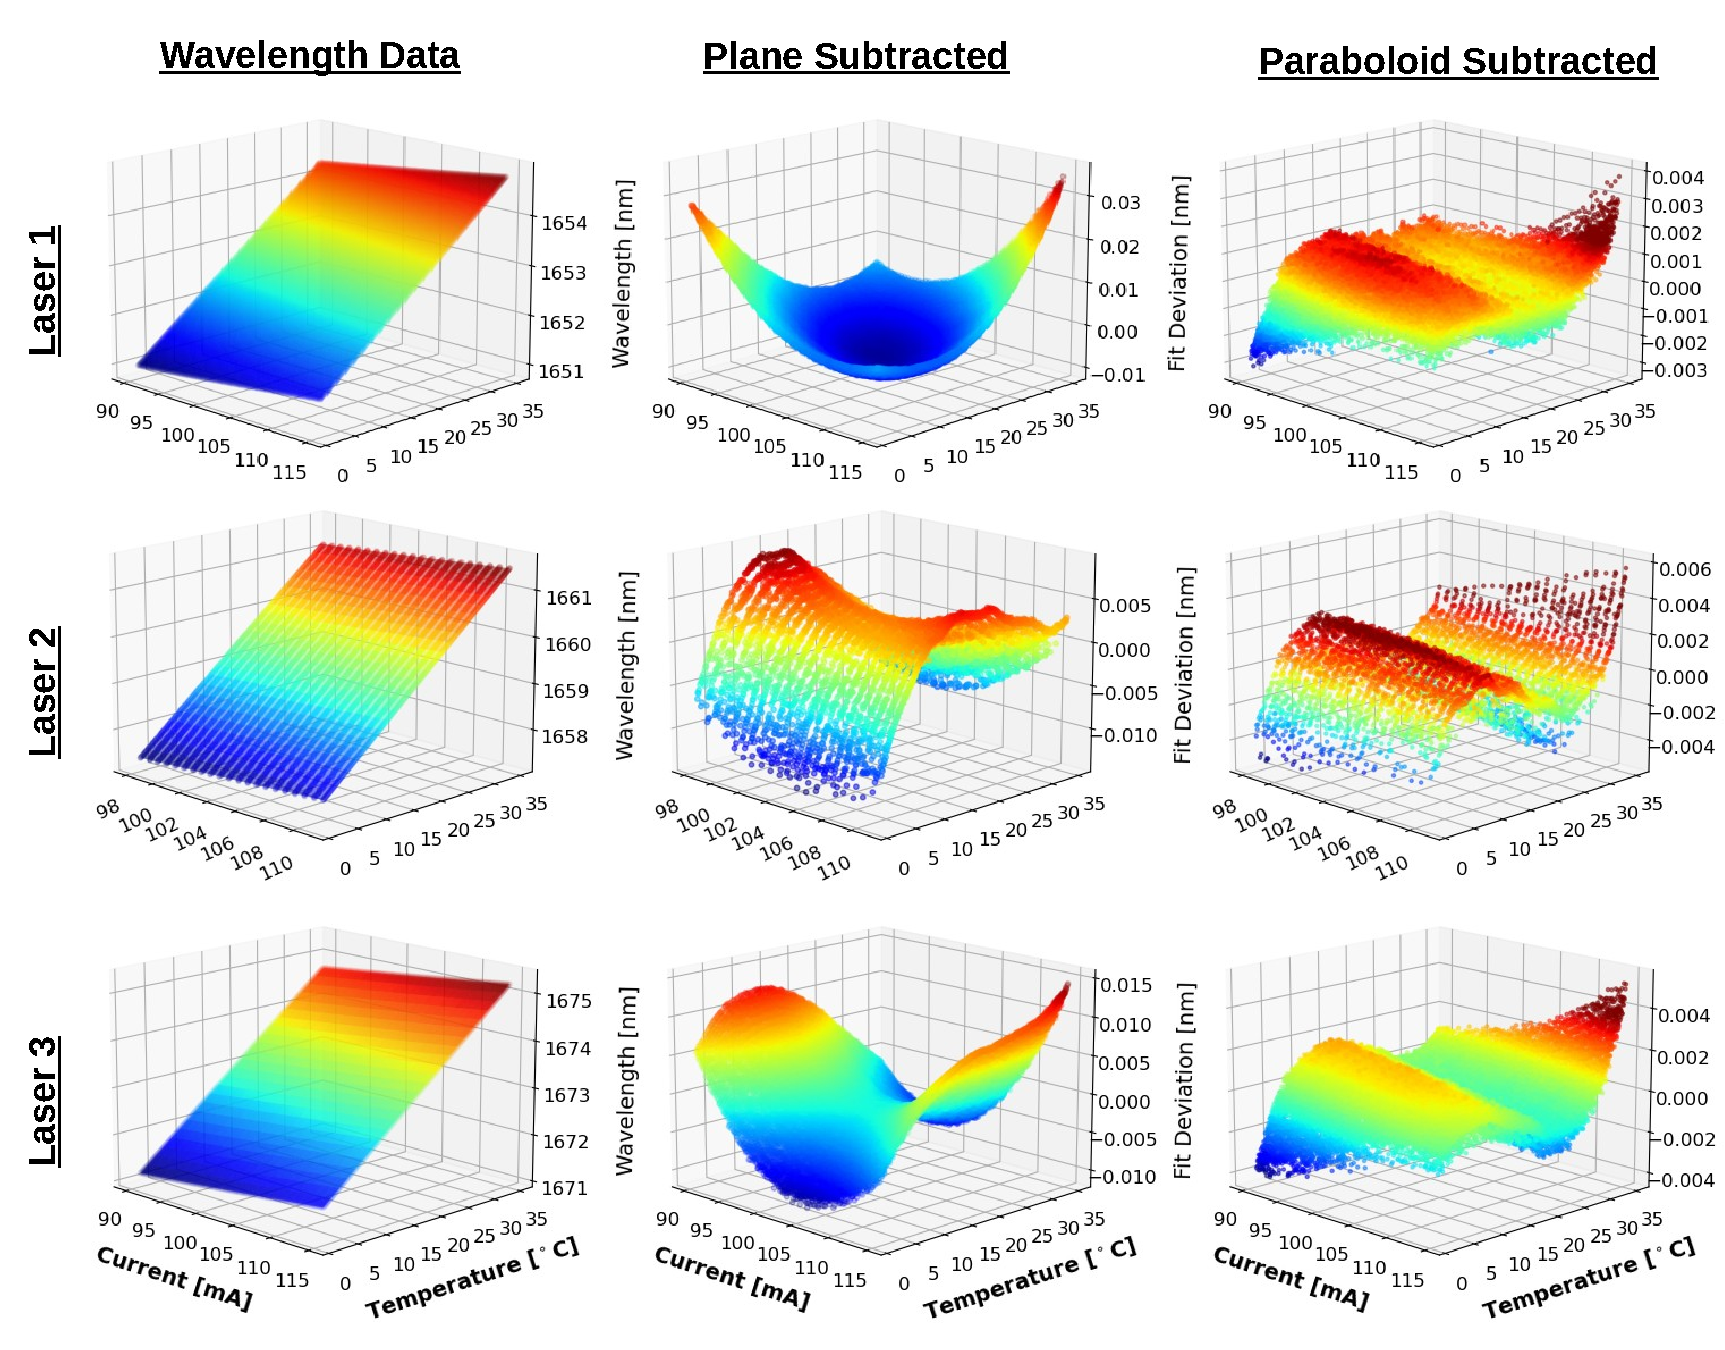
\includegraphics[width=1.0\linewidth]{diagrams/det_laserDetuningPlots}
		\caption{Plot of wavelength against the temperature and injection current for several DFB laser diodes. The lasers each are shown  in the different rows, each corresponding to entries in \ref{table:diodes}. In each column, from left to right, the shown plots are: the row detuning data (left), the residual of this data from the P3 plane fit (middle), and the residual from the Q6 quadratic form fit (right). The polar decomposition variables $\phi$ and $\alpha$ represent the orientation of the planar component of this surface, and the angle $\theta$ represents the orientation of the quadratic surface that superimposes on the planar component.}
		\label{fig:det_detuningsurface}
	\end{figure}
	
	\subsection{Principal Axis Decomposition and the E3 Model}
	In this work, we move beyond treating wavelength as an external independent variable, instead treating it as a set of coupled parameters within a global optimization problem. While the $Q6$ quadratic model provides a comprehensive description of the tuning manifold, its high dimensionality allows for overfitting and the obscuring of residual features. To mitigate this and further stabilize the optimization process, we leverage the spectral theorem to perform a principal axis decomposition of the $Q6$ quadratic form.
	
	The Q6 quadratic tuning model given by (\ref{det_quadratic}) can be written as
	\begin{equation}
		\lambda_\mathrm{Q6}(I, T; \vec{\mathbf{a}}) = \vec{\mathbf{p}}^T \mathbf{M} \vec{\mathbf{p}}
	\end{equation}
	Where $\vec{\mathbf{p}} = [I, T, 1]^T$ is the vector of input parameters and $\mathbf{M}$ is the symmetric coefficient matrix
	\begin{equation} \label{det_coeff_mat_a}
		\mathbf{M}(\vec{\textbf{a}}) = 
		\begin{pmatrix}
			a_3 & a_5/2 & a_1/2 \\
			a_5/2 & a_4 & a_2/2 \\
			a_1/2 & a_2/2 & a_0 \\
		\end{pmatrix}
	\end{equation}
	Since the matrix $\mathbf{M}$ in Equation (\ref{det_quadratic}) is real and symmetric, it is orthogonally diagonalizable. By applying the spectral decomposition $\mathbf{M} = \mathbf{X}\mathbf{D}\mathbf{X}^T$, where $\mathbf{D}$ is a diagonal matrix of eigenvalues $\{d_0, d_1, d_2\}$ and $\mathbf{X}$ is an orthogonal matrix of eigenvectors $\{\vec{\mathbf{e}}_0, \vec{\mathbf{e}}_1, \vec{\mathbf{e}}_2\}$, we can transform the parameter vector into a new coordinate system
	\begin{equation}
		\vec{\mathbf{v}} = \mathbf{X}^T \vec{\mathbf{p}}
		\qquad \qquad
		v_i = \left(\vec{\textbf{e}}_i\right)_0 I + \left(\vec{\textbf{e}}_i\right)_1 T + \left(\vec{\textbf{e}}_i\right)_2
	\end{equation}
	In this transformed basis, the quadratic form simplifies to a much more compact, three-parameter model, which we refer to as the $E3$ representation
	\begin{equation} \label{det_eigenModel}
		\lambda_\mathrm{E3}(I, T;\; \vec{\textbf{d}}) = d_0 v_0^2 + d_1 v_1^2 + d_2 v_2^2
	\end{equation}
	
	While the $E3$ model is mathematically equivalent to the $Q6$ model given by (\ref{det_quadratic}), this decomposition allows us to implement a hierarchical optimization strategy. We treat the eigenvectors in $\mathbf{X}$ as global, device-specific constants, while treating the eigenvalues $\{d_i\}$ as local, measurement-dependent variables. In this hierarchy, $\mathbf{X}$ represents the intrinsic "geometry" of the laser's tuning manifold—the principal axes along which temperature and current most strongly couple to wavelength. This geometry is assumed to be a characteristic property of the specific DFB diode and remains invariant across experimental runs. Conversely, the eigenvalues $\{d_i\}$ represent the scaling factors (or "stiffness") of the tuning response, which account for measurement-to-measurement fluctuations such as environmental temperature changes and laser device aging.
	
	%While the $E3$ model is mathematically equivalent to the $Q6$ formulation, this decomposition places the coefficients on two fundamentally different physical footings. We propose a hierarchical optimization strategy: we treat the eigenvectors in $\mathbf{X}$ as global, device-specific constants, while treating the eigenvalues $\{d_0, d_1, d_2\}$ as local, measurement-dependent variables.
	
	%By performing a global optimization over a large ensemble of spectral scans to determine $\mathbf{X}$, we effectively "lock" the orientation and curvature of the tuning surface. For any individual scan, the nonlinear optimizer is then tasked only with searching for the three $d_i$ parameters. This reduction in dimensionality prevents over-fitting to noise, reduces correlations between the fit parameters, as well as makes the fitting process more efficient.
	\begin{table}[H] 
		\begin{center}
			\caption{Eigenvector decomposition of quadratic form fit to laser detuning behavior. Although a total of 12 coefficients are generated for each laser in this manner, they are related by only six independent parameters. It can be seen that the eigenvectors follow a distinct geometry where we have approximately $\vec{\textbf{e}}_0 \sim \left\{ 0 \; 0 \; 1 \right\}^T$. The explicit mapping to the three independent parameters $\theta$, $\alpha$, and $\phi$ is given by (\ref{det_eigen_rotation}) }\label{table:det_fit_eigenvectors}
			\setlength{\extrarowheight}{3pt} % Space for exponentials
			\begin{NiceTabular}{|l|l|}
				\hline
%				\rowcolor{gray!30}
				\multicolumn{2}{|c|}{\rowcolor{gray!40} Laser 1} \\ \hline
				\rowcolor{gray!10} $d_i$ & $v_i$ \\ \hline
				$1650.0213$ & $\left(6.214\cdot 10^{-7}\right) I + \left(2.705\cdot 10^{-5}\right) T + 1.000$ \\ \hline
				$1.058\cdot10^{-4}$ & $\left(7.889\cdot 10^{-1}\right) I + \left(6.145\cdot 10^{-1}\right) T - 1.711\cdot10^{-5}$ \\ \hline
				$3.281\cdot10^{-5}$ & $\left(6.145\cdot 10^{-1}\right) I - \left(7.889\cdot 10^{-5}\right) T + 2.096\cdot10^{-5}$ \\ \hline
			\end{NiceTabular}
			\begin{NiceTabular}{|l|l|}
				\hline
				\multicolumn{2}{|c|}{\rowcolor{gray!40} Laser 2} \\ \hline
				\rowcolor{gray!10} $d_i$ & $v_i$ \\ \hline
				$1655.8156$ & $\left(6.214\cdot 10^{-7}\right) I + \left(2.705\cdot 10^{-5}\right) T + 1.000$ \\ \hline
				$9.545\cdot10^{-5}$ & $\left(9.969\cdot 10^{-1}\right) I + \left(7.711\cdot 10^{-2}\right) T - 4.123\cdot10^{-6}$ \\ \hline
				$-4.404\cdot10^{-5}$ & $\left(7.811\cdot 10^{-2}\right) I - \left(9.969\cdot 10^{-1}\right) T + 3.327\cdot10^{-5}$ \\ \hline
			\end{NiceTabular}
			\begin{NiceTabular}{|l|l|}
				\hline
				\multicolumn{2}{|c|}{\rowcolor{gray!40} Laser 3} \\ \hline
				\rowcolor{gray!10} $d_i$ & $v_i$ \\ \hline
				$1670.0210$ & $\left(1.450\cdot 10^{-6}\right) I + \left(3.093\cdot 10^{-5}\right) T + 1.000$ \\ \hline
				$7.059\cdot10^{-5}$ & $\left(9.886\cdot 10^{-1}\right) I + \left(1.502\cdot 10^{-1}\right) T - 6.080\cdot10^{-6}$ \\ \hline
				$-2.446\cdot10^{-5}$ & $\left(1.502\cdot 10^{-1}\right) I - \left(9.887\cdot 10^{-1}\right) T + 3.036\cdot10^{-5}$ \\ \hline
			\end{NiceTabular}
		\end{center}
	\end{table}
	
	In the experimental detuning profiles observed in Fig. \ref{fig:det_detuningsurface}, the $Q6$ model is fit to the data, and the principal axis decomposition is applied to extract the resulting eigenvalues and eigenvectors. As shown in Table \ref{table:det_fit_eigenvectors}, for all investigated lasers, there exists a persistent eigenvector $\vec{\mathbf{e}}_0$ nearly parallel to the $\{0, 0, 1\}^T$ direction. The $E3$ model's $v_{1,2}$ components essentially capture the quadratic "stiffness" of the tuning relative to this baseline.
	
	%\hl{This decomposition allows us to partition the laser's tuning parameters into two distinct physical categories: \textit{Fingerprint Parameters} and \textit{Dynamic Parameters}... }
	
	%The rotation angles $\alpha$, $\phi$, and the primary orientation $\theta$ represent the "Fingerprint" of the device. These are structural constants determined by the hardware geometry—specifically, how the electrical and thermal axes are oriented relative to the laser's optical cavity. By performing extended-range scans across a wide $I\text{-}T$ landscape (as shown in Fig. \ref{fig:det_detuningsurface}), these angles can be extracted as intrinsic, device-specific constants. Once these fingerprint parameters are locked, they do not need to be re-optimized for subsequent measurements.
	
	The rotation angles $\alpha$, $\phi$, represent the orientation of the plane
	
	Conversely, the eigenvalues $\{d_i\}$ represent the "State" of the laser during a specific scan. These parameters are highly sensitive to transient experimental conditions. We observed that while $d_0$ (the wavelength baseline) effectively tracks ambient temperature shifts and operating conditions, the secondary eigenvalues $d_1$ and $d_2$ exhibit a sensitivity to the temporal dynamics of the measurement itself.
	
	\subsubsection{Polar Coordinate Decomposition of the E3 Model}
	
	For the data shown in Fig. \ref{fig:det_detuningsurface}, the function $\lambda_\mathrm{Q6}(I, T;\; \vec{\mathbf{a}})$ from (\ref{det_quadratic}) is fit to the data, and the principle axis decomposition is used to find the resulting eigenvalues $d_{0,1,2}$ and eigenvectors $\vec{\textbf{e}}_{0,1,2}$. These values are reported in Table \ref{table:det_fit_eigenvectors}, where it can be seen that for all of the plotted lasers, there is an eigenvector nearly parallel to the $\left\{0\;0\;1\right\}^T$ direction. Since the three $\vec{\textbf{e}}_{0,1,2}$ form an orthonormal basis, they are approximately described by
	\begin{align}
		\vec{\textbf{e}}_0 \simeq \begin{Bmatrix} 0 & 0 & 1 \end{Bmatrix}^T &&
		\vec{\textbf{e}}_1 \simeq \begin{Bmatrix} \cos\theta & \sin\theta & 0 \end{Bmatrix}^T &&
		\vec{\textbf{e}}_2 \simeq \begin{Bmatrix} \sin\theta & -\cos\theta & 0 \end{Bmatrix}^T &&
	\end{align}
	The results in Table \ref{table:det_fit_eigenvectors} reflect slight rotations of the above coordinates about the y- and z-axes in this space. This can be seen from the following rotations of the base left-handed coordinates, where the rotations of the above coordinates are conducted with the small angles $\alpha$ and $\phi$. Denoting the rotation matrices $\textbf{R}_x$, $\textbf{R}_y$, and $\textbf{R}_z$ we have
	\begin{align} \label{det_eigen_rotation}
		\textbf{X}^T &= \textbf{R}^{(1)}_z(-\alpha) \textbf{R}^{(1)}_y(-\phi) \textbf{R}_x(\theta)
		\begin{pmatrix}
			0 & 0 & 1 \\
			1 & 0 & 0 \\
			0 & -1 & 0
		\end{pmatrix} \nonumber\\
		&=\left(\begin{matrix}\alpha \cos{\left(\theta \right)} - \phi \sin{\left(\theta \right)} & \alpha \sin{\left(\theta \right)} + \phi \cos{\left(\theta \right)} & 1\\\alpha \phi \sin{\left(\theta \right)} + \cos{\left(\theta \right)} & - \alpha \phi \cos{\left(\theta \right)} + \sin{\left(\theta \right)} & - \alpha\\\sin{\left(\theta \right)} & - \cos{\left(\theta \right)} & \phi\end{matrix}\right) \nonumber\\
		\textbf{X}^T & \simeq
		\left(\begin{matrix}\alpha \cos{\left(\theta \right)} - \phi \sin{\left(\theta \right)} & \alpha \sin{\left(\theta \right)} - \phi \cos{\left(\theta \right)} & 1 \\
		\cos{\left(\theta \right)} &  \sin{\left(\theta \right)} & -\alpha\\
		\sin{\left(\theta \right)} & - \cos{\left(\theta \right)} & \phi\end{matrix}\right)
	\end{align}

	The above analysis leads us to the conclusion that we can reliably extract an arbitrary detuning angle $\theta$ from the eigensystem $\mathbf{M}$ as well as the small deviation angle $\phi$ and $\alpha$. For Laser 3 from Table \ref{table:det_fit_eigenvectors}, the detuning angle is $\tan\theta \simeq \left(1.502 / 9.886\right)$ and the small rotation angles are $\alpha \sim 6.08\cdot10^{-6}$ and $\phi \sim 3.036\cdot10^{-6}$.
	
	Under the above small angle approximation the planar behavior of the E3 model is (\ref{det_eigenModel}) is dominated by the $d_0$ term. This can be seen from carrying out the calculation of the $\vec{\textbf{v}}$ components
	\begin{align} \label{det_polar_decomp}
		v_0^2 &\simeq 2 I \Big(\alpha \cos\theta - \phi \sin \theta\Big) + 2 T \Big(\alpha \sin\theta + \phi \cos\theta \Big) + 1 \nonumber\\
		v_1^2 &\simeq I^2 \cos^2\theta + 2 I T \sin\theta \cos\theta + T^2 \sin^2\theta \nonumber\\
		v_2^2 &\simeq I^2 \sin^2 \theta - 2IT \sin\theta \cos\theta + T^2 \cos^2\theta
	\end{align}
	In the above relations we have dropped the linear $\alpha$ and $\phi$ in the $v{1,2}$ terms since they are multiplied by the $d_{1,2}$, which were very small since the ratios $d_{1,2}/d_0$ were observed to be even smaller than $\alpha$ or $\phi$ in Table \ref{table:det_fit_eigenvectors}.
	
	In the E3 model, as formulated in (\ref{det_coeff_mat_a}), the major plane contribution is not immediately obvious. Using the small angle approximation which resulted in the relations (\ref{det_polar_decomp}), we see that the $\vec{\textbf{e}}_0$ vector gives the approximate normal direction of this plane, and the orientation of the quadratic surface which lives on this plane is set by $\vec{\textbf{e}}_{1,2}$. This situation is depicted in Fig. \ref{fig:det_eigenvector_diagrams}.
	
	\begin{figure}[H]
		\centering
		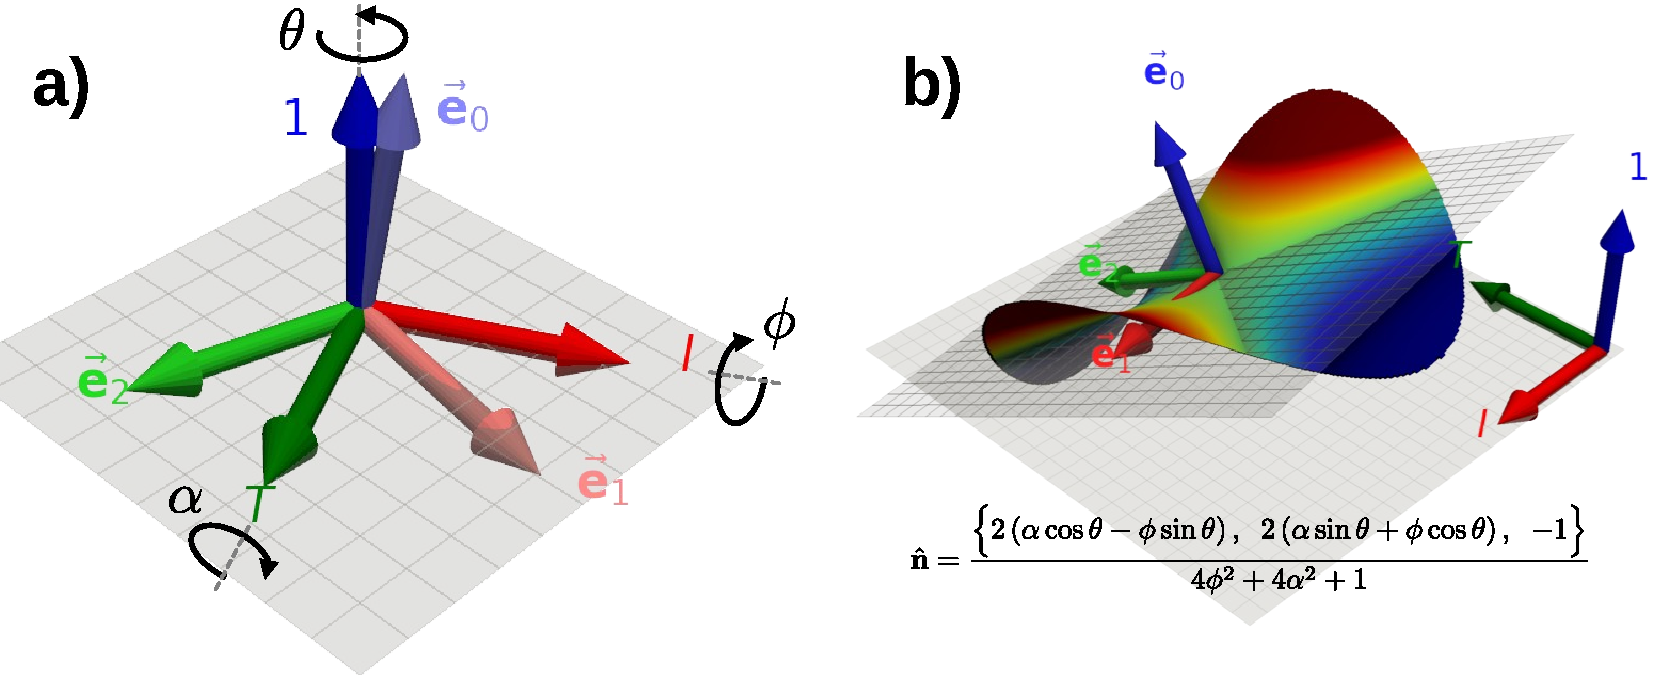
\includegraphics[width=1.0\linewidth]{diagrams/det_eigenvectorDiagrams}
		\caption{Coordinate directions defined by the eigenvectors $\vec{\textbf{e}}_{0-2}$ of the coefficient matrix (\ref{det_coeff_mat_a}) are displayed in \textbf{a)} as rotated from the original $I$ and $T$ coordinate directions. The rotation is performed about the z-axis by an arbitrary angle $\theta$, and small angles $\phi$ and $\alpha$ about the y-and z-axes, respectively. The relation of these eigenvectors to the quadratic detuning surface is shown in \textbf{b)}, where it can be seen that the components of the $\vec{\textbf{e}}_0$ vector give the normal direction of the underlying planar behavior, and the angle $\theta$ gives the orientation of this surface superimposed on top of this plane via the $\vec{\textbf{e}}_{1,2}$ vectors. The normal direction $\hat{\textbf{n}}$ of the plane when plotted in $I-T-\lambda$ coordinates is given.}
		\label{fig:det_eigenvector_diagrams}
	\end{figure}
	
	
	\subsection{The R6 Detuning Model} \label{sec:det_R6}
	
	From the polar decomposition in (\ref{det_polar_decomp}), we can see that the planar behavior is dominated by the term corresponding to the $\left\{0\;0\;1\right\}$ eigenvector. It can be seen that there is no way to adjust the fit offset independently from the terms defining the plane orientation. We propose a new model which retains the polar description of the higher order terms, but allows the planar terms to be defined explicitly
	\begin{align} \label{det_model_R6}
		\lambda_\mathrm{R6}(I, T;\; \vec{\textbf{b}},\theta) = b_0 + b_1 I + b_2 T + b_3 v_1^2 + b_4 v_2^2
	\end{align}
	where the quadratic terms are given by the rotated coordinates
	\begin{align}
		v_1 &= I\cos\theta + T\sin\theta \nonumber\\
		v_2 &= I\sin\theta - T\cos\theta
	\end{align}
	
	\subsubsection{Initial Guess for the Model}
	Unlike the Q6 or P3 detuning models, the model in (\ref{det_model_R6}) is nonlinear in the $\theta$ parameter. A procedure for forming an initial guess for these parameters to measured detuning data can be constructed as follows:
	\begin{itemize}
		\item Perform linear fitting using Q6. We can use the linear decomposition formula (\ref{leastSquares}) to find the coefficients $a_{0-5}$ of the Q6 model to wavelength measured against current and temperature. Since this solution is given explicitly, it does not require an initial guess.
		\item Perform eigenvalue decomposition of the resulting matrix of coefficients (\ref{det_coeff_mat_a}) to give the eigenvalues $d_{0-3}$ and eigenvectors $\vec{\textbf{e}}_{0-3}$, arranged in the order of Table \ref{table:det_fit_eigenvectors}.
		\item From the polar decomposition discussion, we can identify the angle $\theta$ of the quadratic surface using $\tan\theta = (\vec{\textbf{e}}_1)_1 / (\vec{\textbf{e}}_1)_0$, which serves as an initial guess for this angle in the R6 model. The angles giving the plane orientation are $\phi = (\vec{\textbf{e}}_2)_2$ and $\alpha = -(\vec{\textbf{e}}_1)_2$. These angles, along with the eigenvalues, give the guesses for the plane coefficients
		\begin{align}
			b_0 \sim d_0 && b_1 \sim 2d_0\left(\alpha \cos\theta - \phi \sin \theta\right) && b_2 \sim 2d_0 \left(\alpha \sin\theta + \phi \cos\theta\right) && b_3 \sim d_1 && b_4 \sim d_2
		\end{align}
	\end{itemize}
	
	\subsection{The R9 Detuning Model}
	\begin{align} \label{det_model_R9}
		\lambda_\mathrm{R9}(I, T;\; \vec{\textbf{b}},\theta, \theta_2) = b_0 + b_1 I + b_2 T + b_3 v_1^2 + b_4 v_2^2 + b_5 v_3^3 + b_6 v_4^3
	\end{align}
	where the quadratic and cubic terms are given by the independently rotated coordinates
	\begin{align}
		v_1 &= I\cos\theta + T\sin\theta &&& v_3 &= I\cos\theta_2 + T\sin\theta_2 && \nonumber\\
		v_2 &= I\sin\theta - T\cos\theta &&& v_4 &= I\sin\theta_2 - T\cos\theta_2 &&
	\end{align}
	\section{Investigation of the Dynamic Tuning Profile}
	The purpose of this section is to investigate the performance of the detuning models in describing the performance of a laser under actual scan conditions. We can directly evaluate the fitting performance of the various models on directly measured wavelength data before proceeding to the measurement-less scheme.
	
	For this benchmark, we analyze data taken using \textbf{Laser 3} in the setup that was shown in Fig. \ref{fig:crds_experimentalsetup_nopc}. During the course of the investigation in Ch. \ref{chap:acetone}, we collected many datasets have which have recordings of DFB laser wavelength against laser current $I$ and temperature $T$. By analyzing an ensemble of datasets collected with varying scan durations (as shown in Fig. \ref{fig:crds_experimentalsetup_nopc}), we identified a previously unobserved correlation between the tuning geometry and the scan rate.
	
	For each scan encompassing a range of wavelengths, we fit the surface of detuning behavior to one of the previously described models. Prior to fitting, we recenter the control variables $I$ and $T$ on some average value which is well centered within the dataset:
	\begin{align}
		I \rightarrow \bar{I} =  I - I_0 && T \rightarrow \bar{T} =  T - T_0
	\end{align}
	This helps to reduce correlations between the model coefficients.
	
	\subsection{Quadratic Form (Q6) and Planar (P3) Fits}
	For each scan in the dataset, the P3 model from (\ref{det_plane_P3}) and the Q6 model from (\ref{det_quadratic}) were both fit using the recorded current and temperature values from the laser current controller against the measured wavelength values. For all datasets, the correlation plots of the $a_{0-2}$ for the P3 as well as the $a_{0-5}$ for the Q6 fits are shown in Fig. \ref{fig:det_crosscorrelations_combined}.
	
	The planar P3 coefficients were relatively stable, showing a pronounced correlation between the $a_1$ and $a_0$ coefficients. We do not pursue the interpretation of these fluctuations in detail, as the P3 model provides a poor description of the tuning profile.
	
	The coefficients which resulted from the quadratic form fit Q6 did not show clear trends in the correlation plots, as can be seen from \ref{fig:det_crosscorrelations_combined}. The values of the coefficients corresponding to the quadratic terms showed large fluctuations, and the interpretation of these fluctuations was not clear in these coordinates.
	
	It was found that the fluctuations of the $a_0$ coefficient of the Q6 quadratic fit did show some structure when plotted against time. This can be seen in Fig. \ref{fig:det_correlation_date_q6}. These fluctuations were attributed to changing lab ambient conditions.
	\begin{figure}[H]
		\centering
		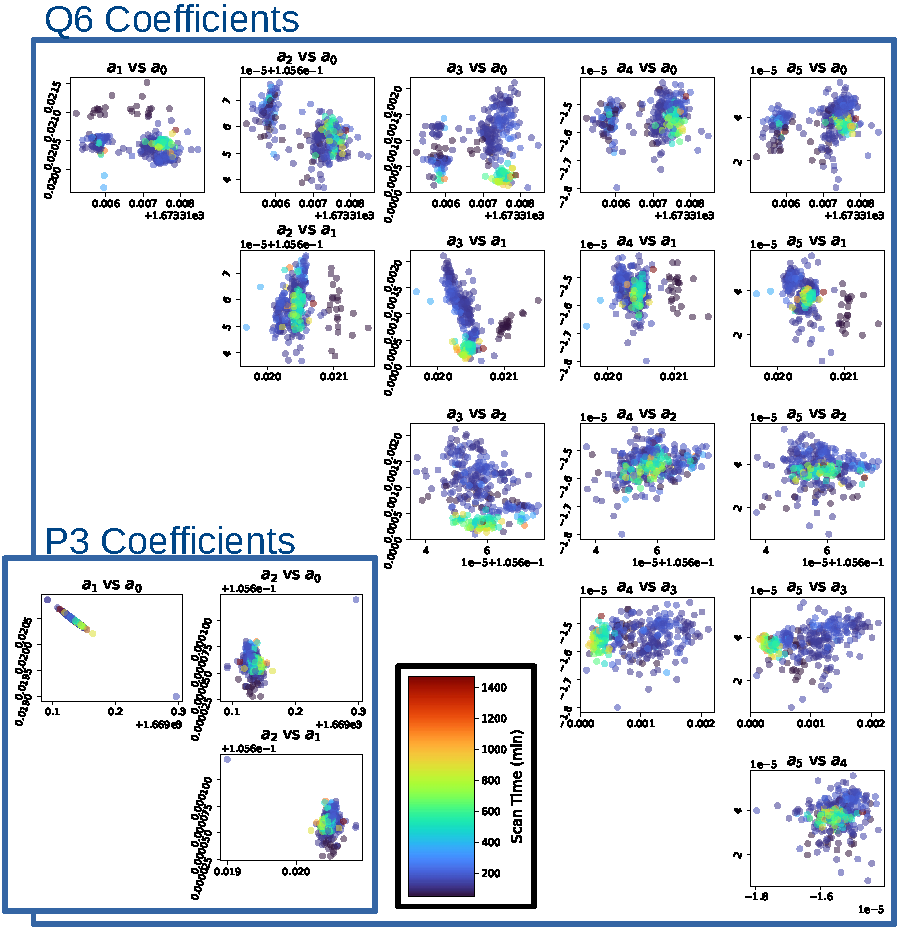
\includegraphics[width=1.0\linewidth]{diagrams/det_crossCorrelations_combinedP3-Q6}
		\caption{Correlation plots of the parameters obtained by fitting the Q6 and P3 models to detuning data from \textgreater 300 laser scans. The quadratic terms obtained by fitting the Q6 model were not particularly stable.}
		\label{fig:det_crosscorrelations_combined}
	\end{figure}
	
	\begin{figure}[H]
		\centering
		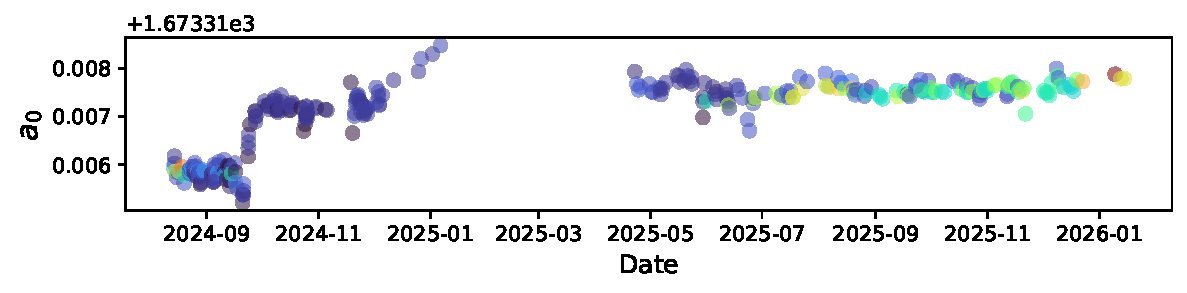
\includegraphics[width=1.0\linewidth]{diagrams/det_date_correlation_Q6}
		\caption{Fluctuation of the offset term $a_0$, obtained by fitting the ensemble of scan data with the Q6 detuning model (\ref{det_quadratic}). These fluctuations seemed to show structure only when plotted against the date that each scan was performed, indicating a contribution from changing ambient conditions.}
		\label{fig:det_correlation_date_q6}
	\end{figure}
	
	
	\subsection{Eigenvector Decomposition (E3) and the Polar R6 Model}
	For each of the six $a_{a-5}$ coefficients obtained from fitting the Q6 model to an ensemble of scanning data, the eigenvalue decomposition was performed to obtained the eigenvalues $d_{0-2}$ and eigenvectors $\vec{\textbf{e}}_{0-2}$. The polar decomposition gives the three independent angles which give the orientation of these eigenvectors
	\begin{align}
		\theta = \tan^{-1}\Big[(\vec{\textbf{e}}_1)_1 \big/ (\vec{\textbf{e}}_1)_0\Big] && \phi = (\vec{\textbf{e}}_2)_2 && \alpha = -(\vec{\textbf{e}}_1)_2
	\end{align}
	Performing this decomposition on the six coefficients obtained from the Q6 fit to each scan in the dataset gives a transformed set of parameters. The correlations between these transformed parameters is shown in Fig. \ref{fig:det_crosscorrelations_E3R6}, where several new patterns emerge.
	
	The correlations between $\theta$, $\phi$, and $\alpha$ reveal that these three parameters live tightly along a curve in 3-D space, indicating that all three are determined by one parameter. Additionally, there are several correlations between the polar angles and $d_{0,1}$. This can be interpreted as a coupling of the orientation of the quadratic surface to one of the other parameters. To further investigate this coupling, we proceed to re-fit this data using the R6 model.
	
	For the same datasets, a new set of coefficients is obtained by nonlinear fitting of the R6 model to the measured $IT-\lambda$ data. Because the $\theta$ parameter appears nonlinearly in the model, we cannot use the one-step fitting of equation (\ref{leastSquares}). For this, we used the Levenberg-Marquandt algorithm with an initial guess constructed from the earlier Q6 fits using the method described earlier in Sec. \ref{sec:det_R6}. The results of this process is shown by the correlation plots of Fig. \ref{fig:det_crosscorrelations_E3R6}. It can now be clearly seen that there is a systematic correlation between $b_3$ and $\theta$ in the R6 model. Geometrically, this means that the stretch $b_3$ of the quadratic surface varies in a predictable manner with the angle $\theta$ representing the rotation of the surface.
	
	The appearance of this correlation in three of the fit models is displayed in Fig. \ref{fig:det_correlation_d-theta}. For each of these correlations, it was found that functions of the form
	\begin{align} \label{det_dynamic_AB_relation}
		\theta(d_1) = \frac{A}{d_1} + B &&\text{and}&& \theta(b_3) = \frac{A}{b_3} + B &&
	\end{align}
	fit well to the correlation plots for the E3 and R6 parameters, respectively. Furthermore, the values of $A$ and $B$ extracted from these curve fits was consistent between the E3 and R6 parameters, seeming to indicate that these values result from some intrinsic property of the laser device.
	
	The appearance of this $\theta(d_1)$ or $\theta(b_3)$ curve is only manifest under an ensemble of many fits to the laser detuning behavior. We can think of the $A$ and $B$ in relation (\ref{det_dynamic_AB_relation}) as the \textit{dynamic tuning} coefficients, which relate the curvature and orientation of the dominant quadratic component of the tuning surface.
	
	To further investigate if the relation between $\theta$ and the scaling factor of the detuning surface persists as we attempt to model higher order behavior, we proceed to investigate whether this correlation persists under the cubic R9 model.
	
	
	\begin{figure}[H]
		\centering
		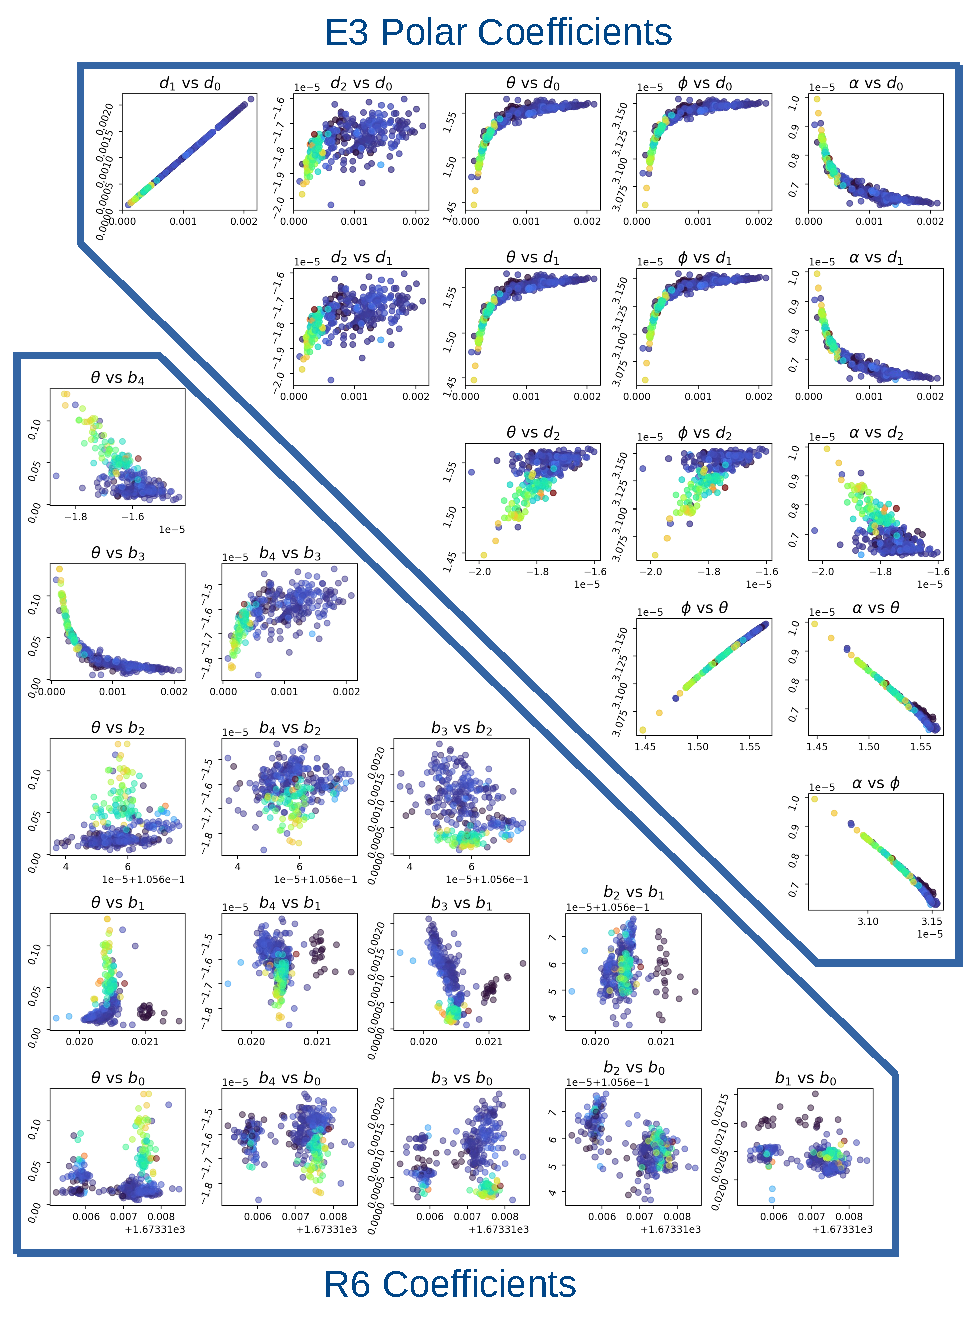
\includegraphics[width=1.0\linewidth]{diagrams/det_crossCorrelations_combinedE3-R6}
		\caption{Correlation plots between the parameters of the R6 and polar E3 models, obtained from fits to an ensemble of many scans.}
		\label{fig:det_crosscorrelations_E3R6}
	\end{figure}
	
	
	\begin{figure}[H]
		\centering
		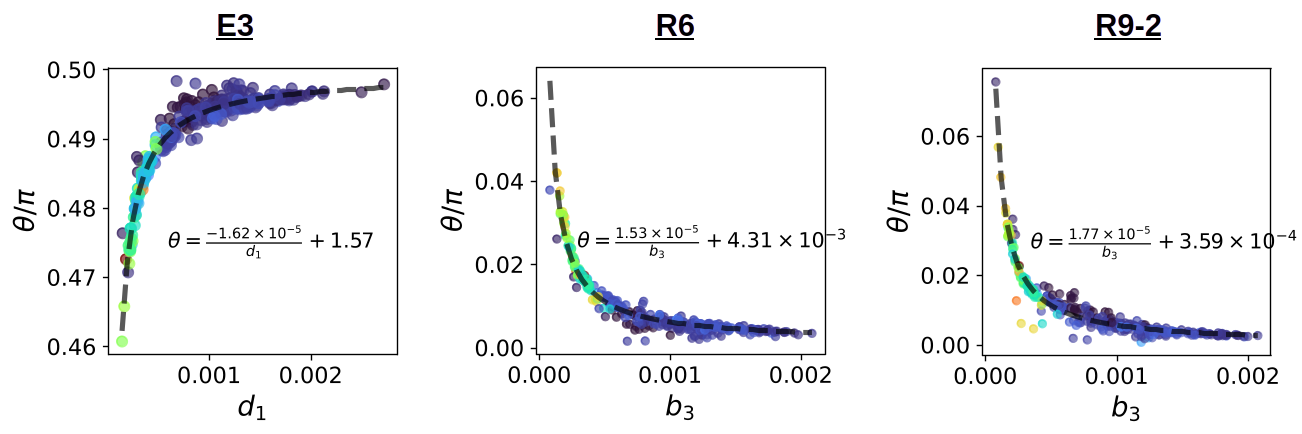
\includegraphics[width=1.0\linewidth]{diagrams/det_correlation_d-theta}
		\caption{Correlation plots between the orientation angle $\theta$ of the quadratic surface and the curvature of this surface, given by $d_1$ for the E3 model and $b_3$ for the R6 and R9-2 models. The coefficient in the numerator of the fit equation is similar in magnitude between the three models, hinting at an effect which is intrinsic to the laser device and not an artifact of the coordinates used. Since this effect only appears across an ensemble of different scans and seems to correlate with the scan rate (shown by the point colors), the numerator coefficient is dubbed the \textit{dynamic tuning coefficient}. }
		\label{fig:det_correlation_d-theta}
	\end{figure}
	
	\subsection{Investigating the Cubic Contribution -- Fitting the R9 Model}
	The cubic behavior of the tuning profile can be seen from the residual plots in Fig. \ref{fig:det_detuningsurface}, where all three lasers can be seen exhibit cubic contributions which are about an order of magnitude less than the quadratic contributions. At the expense of three additional coefficients, the cubic terms present in the R9 model are able to account for the remaining structured residuals in the measured wavelength data.
	
	We investigate the stability of the coefficients when fitting an ensemble of scans using the R9 model. This serves two purposes: to develop a more accurate detuning model which will serve well in the next section, and to investigate whether the correlation shown in Fig. \ref{fig:det_correlation_d-theta} persists in this more advanced model.
	
	This analysis was performed by performing a nonlinear fit of the R9 model to each measured detuning profile in the dataset. An initial guess for the fit parameters was formed from the previously performed R6 fit, setting the remaining coefficients to zero. Correlation plots of the parameters revealed that the 9 coefficients of the R9 model did not stabilize on definite values for our scans. This is partially due to the fact that most of the scans in the ensemble were conducted on a smaller range of currents than those shown in Fig. \ref{fig:det_detuningsurface}. This narrow scan range creates a condition of overfitting for many of the scans.
	
	To proceed with the analysis, we chose to fix two of the fit parameters to values obtained from the broad detuning data in Fig. \ref{fig:det_detuningsurface}. For this, we choose to fix $\theta_2$ and the ratio $b_5 / b_6$. The reasoning for this choice is that for scan which encompass a more narrow range of currents, the orientation of the cubic contributions may not be as resolvable as in the more broad range scans. This then leads us to the reduced parameter R9 model, containing 7 fit parameters
	\begin{equation}
		\lambda_\mathrm{R9\text{-}2}(I, T;\; \vec{\textbf{b}},\theta) = b_0 + b_1 I + b_2 T + b_3 v_1^2 + b_4 v_2^2 + b_5( v_3^3 + \epsilon v_4^3 )
	\end{equation}
	Here the angle $\theta_2$, which defines $v_{3,4}$, and the ratio $\epsilon = d_6 / d_5$ are both held fixed.
	
	When using the R9-2 model to perform the analysis of directly measured detuning data, there were no significant correlations between the fit parameters other than the $\theta-d_3$ correlation shown in Fig. \ref{fig:det_correlation_d-theta}, which remained strong and was well fit by (\ref{det_dynamic_AB_relation}). For this reason, we refrain from displaying the whole table of correlation plots. The dynamic tuning relation (\ref{det_dynamic_AB_relation}) was well preserved across all three models, indicating that this must be related to the intrinsic device characteristics.
	
	We perform one additional reduction of the R9-2 model by enforcing the dynamic tuning relation (\ref{det_dynamic_AB_relation}) to eliminate the quadratic orientation angle $\theta$ as a fitting parameter. This gives the R9-3 model, a six parameter cubic model of the laser detuning
	\begin{equation}
		\lambda_\mathrm{R9\text{-}3}(I, T;\; \vec{\textbf{b}}) = \lambda_\mathrm{R9\text{-}2}\left(I, T;\; \vec{\textbf{b}},\theta = \frac{A}{b_3} + B\right)
	\end{equation}
	
	The correlation plots of the resulting parameters obtained from fitting the entire dataset is shown in Fig. \ref{fig:det_crosscorrelations_R9-3}.
	
	
%	\begin{figure}[H]
%		\centering
%		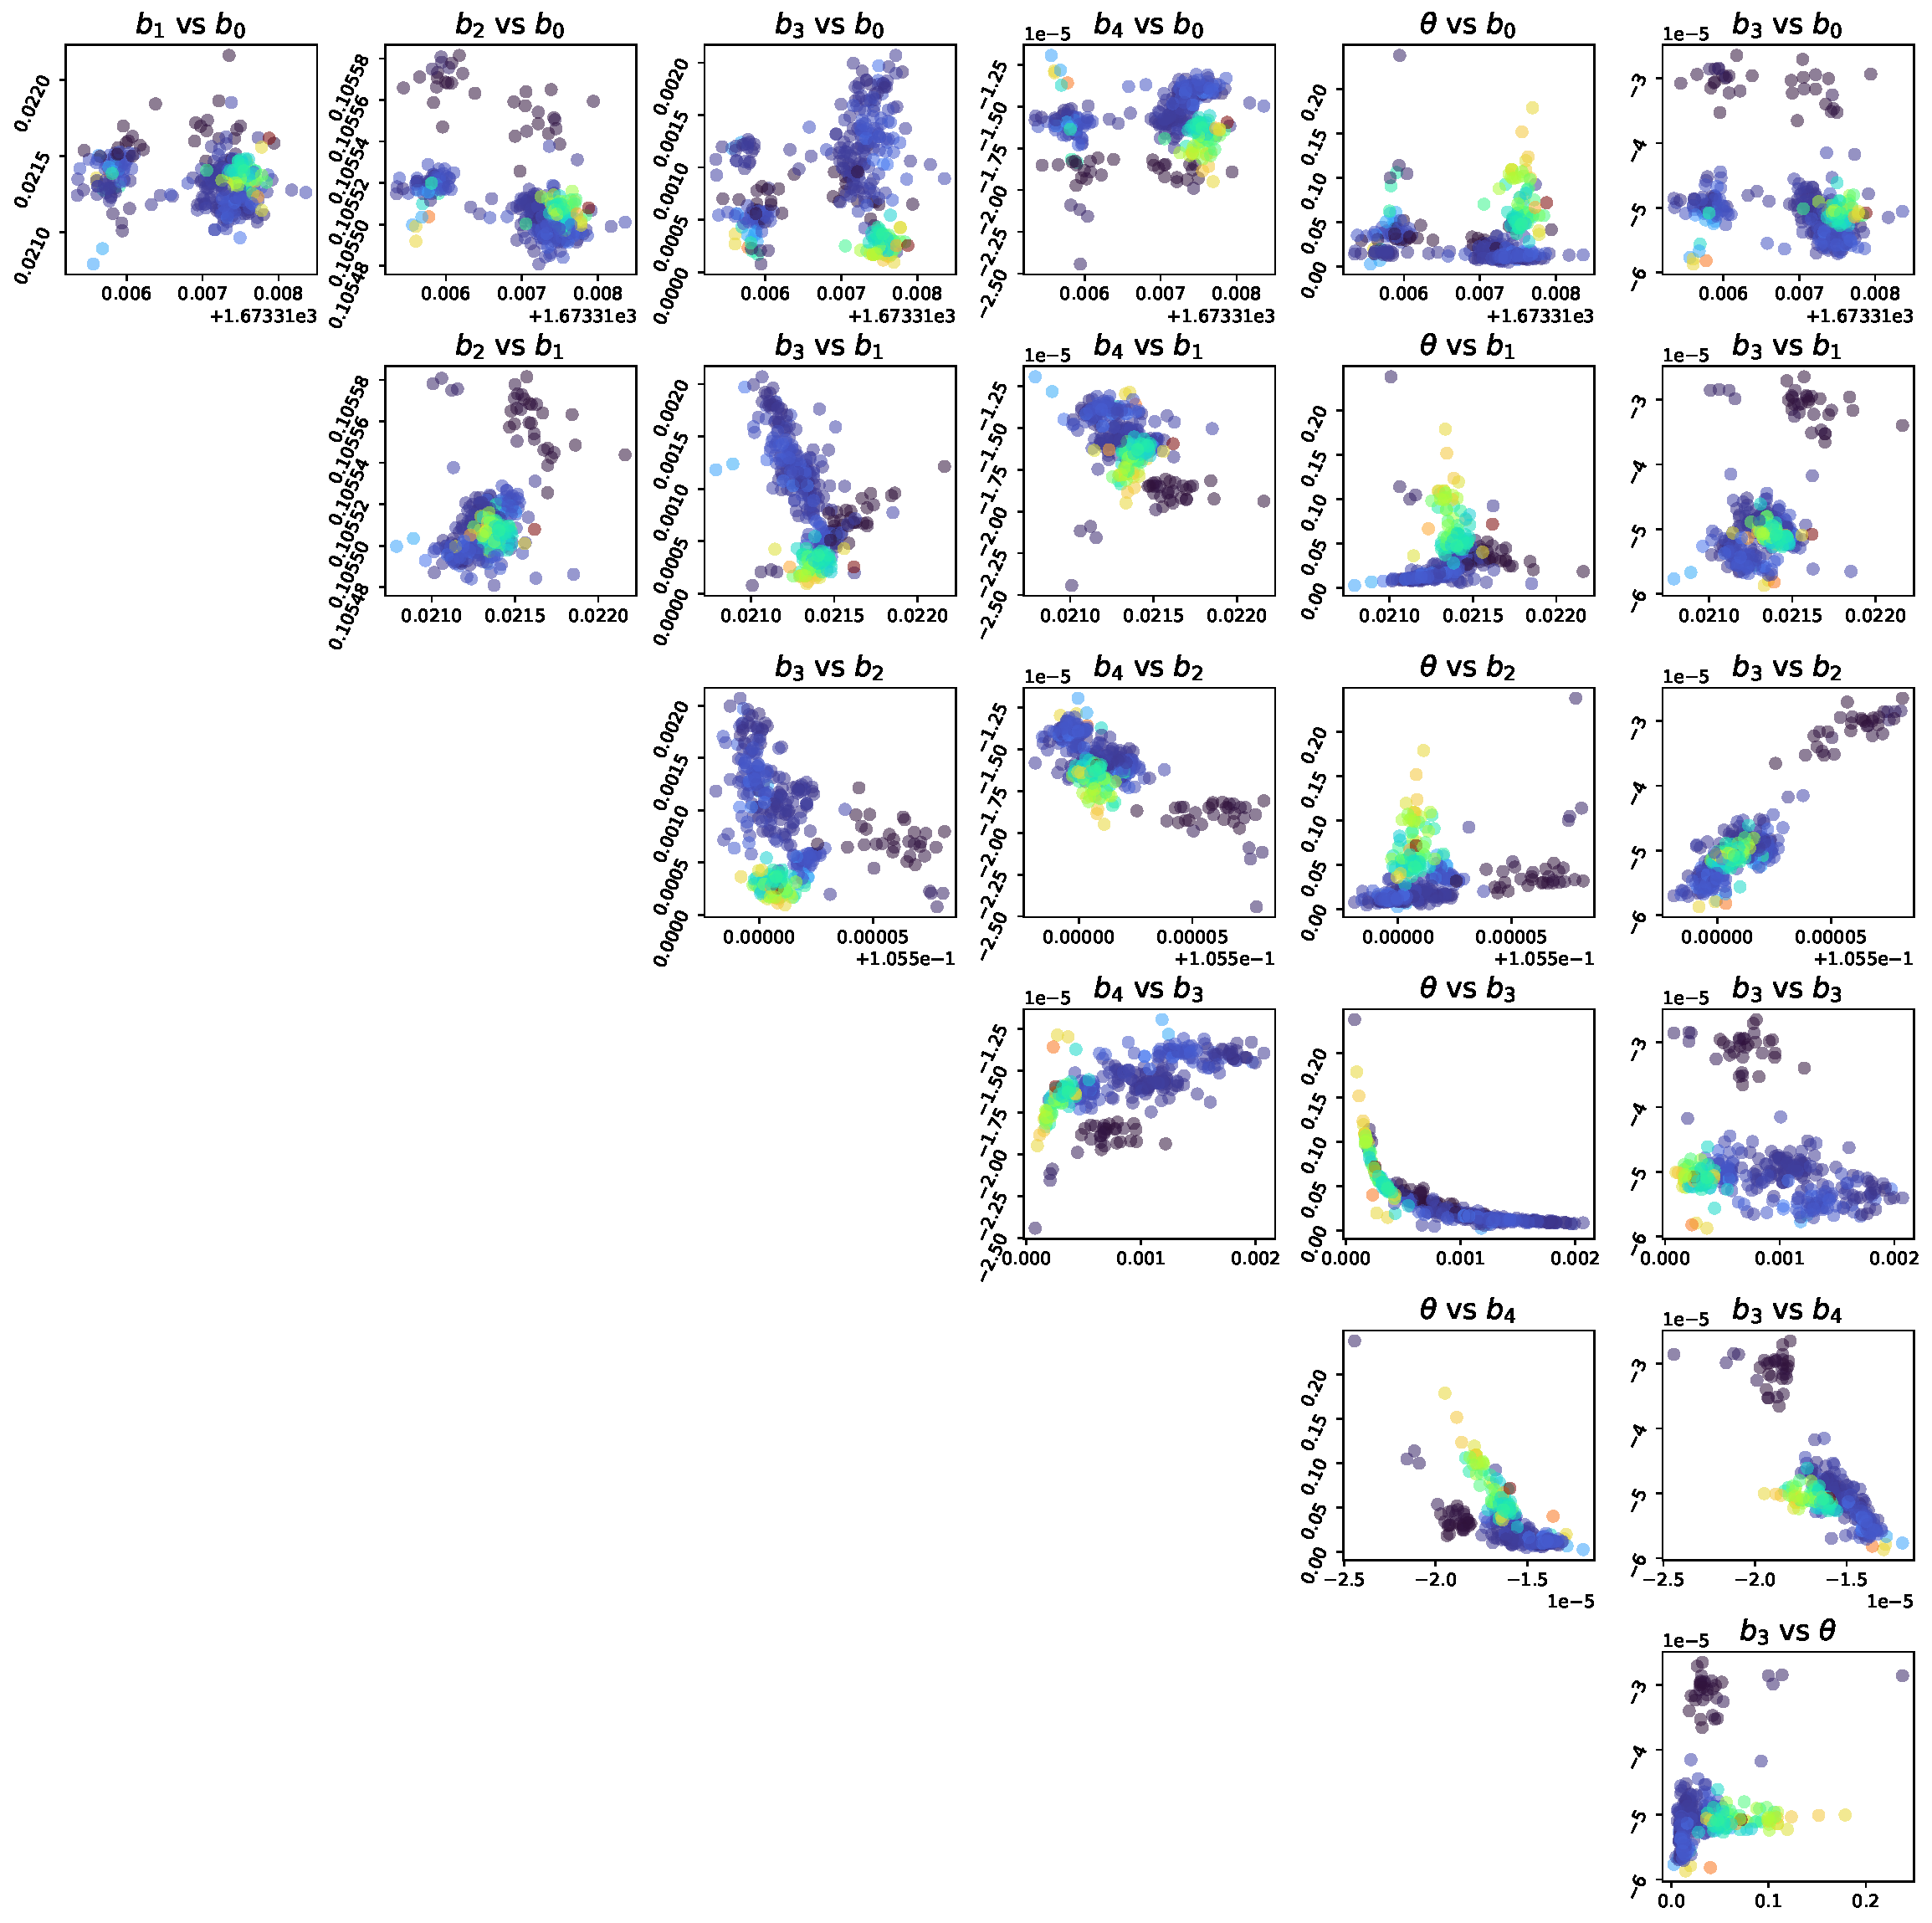
\includegraphics[width=1.0\linewidth]{diagrams/det_crossCorrelations_R9-2}
%		\caption{Correlations of the R9-2 model.}
%		\label{fig:det_crosscorrelations_R9-2}
%	\end{figure}

	\begin{figure}[H]
		\centering
		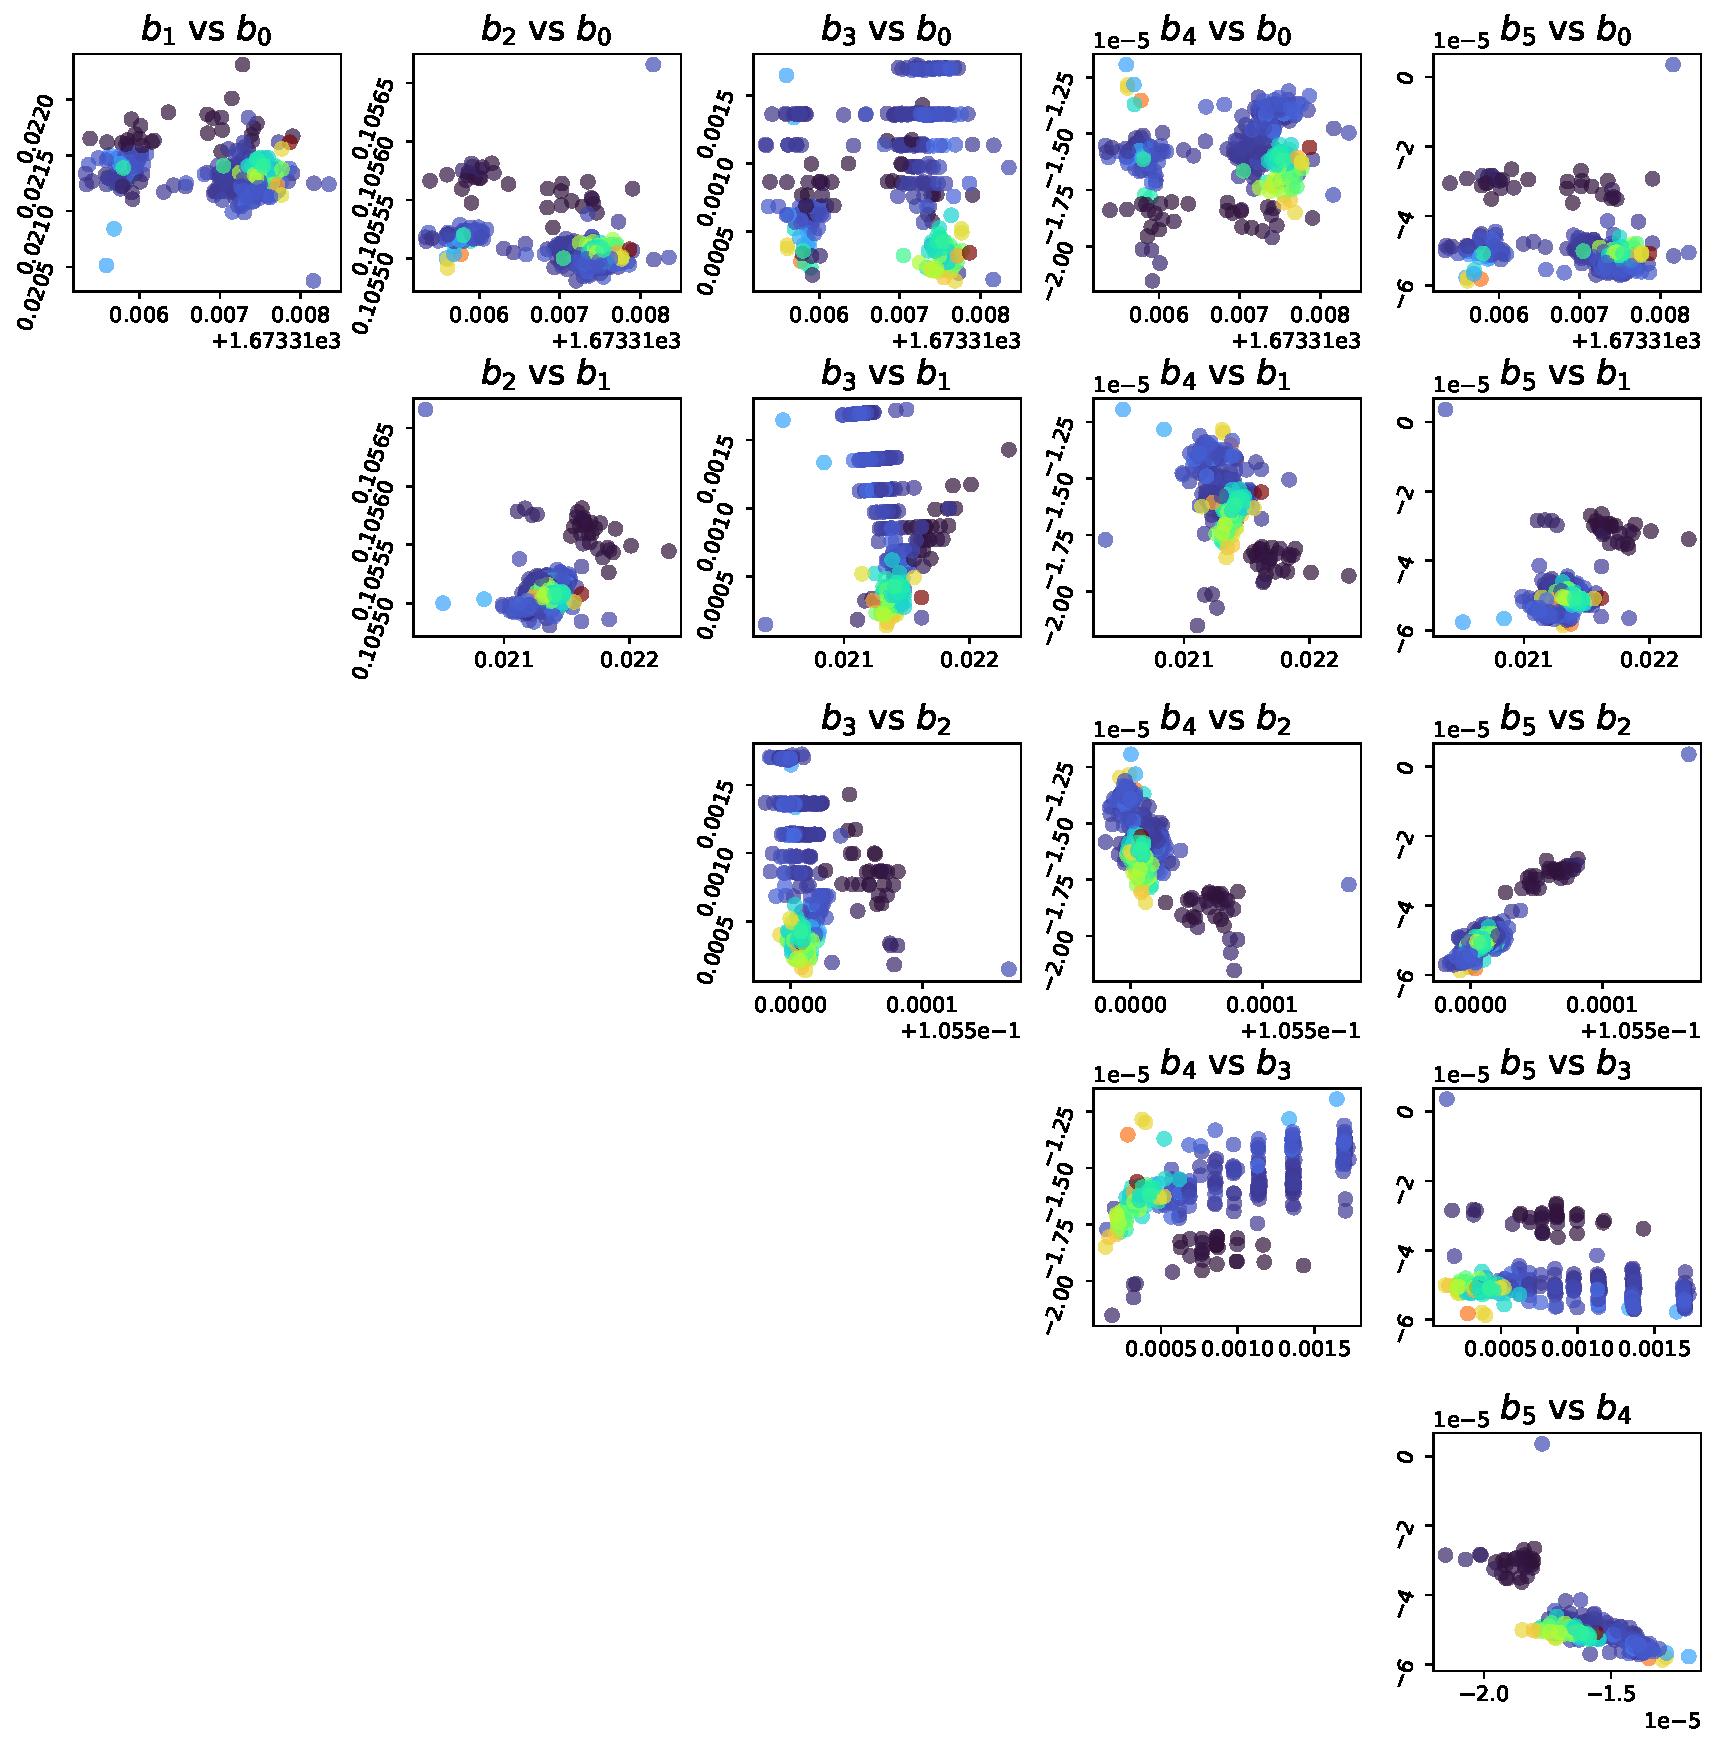
\includegraphics[width=1.0\linewidth]{diagrams/det_crossCorrelations_R9-3}
		\caption{Correlations of the R9-3 model.}
		\label{fig:det_crosscorrelations_R9-3}
	\end{figure}
	
	
	\section{Algorithm for Extraction of the Detuning Coefficients}
	
	The coefficients $\mathbf{a} = \{a_0, \dots, a_{m-1}\}$ in the detuning model characterize the specific response of a laser diode under a given set of environmental and operational conditions. Because these coefficients are subject to transient fluctuations, such as changes in ambient temperature and laser aging, it is not feasible to rely on a static calibration. Instead, we require an automated procedure capable of extracting the optimal detuning coefficients for each individual spectrum scan in a robust manner.
	
	This extraction process is structured as a \textit{nested optimization problem}. The "inner" problem consists of finding the gas concentrations $\{c_j\}$ that best fit the observed absorption at a fixed wavelength axis. This is an analytical, linear least-squares task with a solution given by Eq. (\ref{leastSquares}). The "outer" problem involves searching the parameter space of $\mathbf{a}$ to minimize the residual between the predicted and measured absorption.
	
	\begin{enumerate}
		\item \textbf{Initialization:} 
		A model architecture is selected (e.g., $Q6$ or $E3$). An initial guess for the vector of coefficients $\mathbf{a}^{(0)}$ is provided, ideally sourced from manufacturer specifications or previously recorded stable scans.
		
		\item \textbf{Wavelength Reconstruction (The Outer Loop):} 
		For a given iteration of the Nelder-Mead simplex, the current estimate of the coefficients $\mathbf{a}^{(k)}$ is used to transform the experimental control parameters $\{I_i, T_i\}$ into a reconstructed wavelength axis:
		\begin{equation}
			\lambda_i = \lambda(I_i, T_i;\, \mathbf{a}^{(k)})
		\end{equation}
		This step defines the independent variable for the concentration estimate.
		
		\item \textbf{Concentration Estimation (The Inner Loop):} 
		With the reconstructed $\lambda_i$ and the measured ringdown times $\tau_i$, we calculate the experimental absorption $\alpha(\tau_i, \tau_0(\lambda_i))$. Using these values, a linear least-squares regression is performed to determine the concentrations $\{c_j\}$ of all target species. This step utilizes the non-iterative decomposition described in Equation (\ref{leastSquares}), ensuring that the inner loop remains computationally efficient.
		
		\item \textbf{Model Error Evaluation:} 
		The predicted model absorption, $\alpha_\mathrm{model}(\lambda_i)$, is constructed using the newly determined concentrations and the established cross-sections $\sigma_j(\lambda_i)$. The scalar objective function $F(\mathbf{a})$ is then evaluated:
		\begin{equation}
			F(\mathbf{a}^{(k)}) = \sum_{i=1}^{N} \Big[\alpha_\mathrm{model}(\lambda_i) - \alpha(\tau_i, \tau_0(\lambda_i))\Big]^2 w^2(\tau_i)
		\end{equation}
		where $w(\tau)$ is the weighting function derived in the previous section and the sum is performed over the $N$ measurements obtained in the scan. The evaluation of the baseline ringdown time $\tau_0(\lambda_i)$ is performed using an empirical fit, as described in Ch. \ref{chap:CRDS}.
		
		\item \textbf{Simplex Update and Convergence:} 
		The Nelder-Mead algorithm evaluates the error at the new vertex, performing reflections, expansions, or contractions to move the simplex toward the global minimum. This process repeats until the change in $F(\mathbf{a}^*)$ falls below a predefined tolerance $\epsilon$, signifying that the coefficients $\mathbf{a}^*$ have reached a stationary value.
		
		\item \textbf{Final Extraction:} 
		Once convergence is achieved, a final pass of the inner loop is performed using the optimized $\mathbf{a}^*$ to produce the definitive concentration estimates for the scan.
		
		\item \textbf{Self-Broadening Iteration:} Upon this first pass of the algorithm, the obtained concentrations are used to calculate a new set of cross sections $\sigma_j(\lambda_i; c_j)$ which take into account the self-broadening contribution to the lineshape. With these updated cross section functions, the algorithm is repeated only a single additional time, as the resultant concentrations come very close to those obtained from the first pass.
	\end{enumerate}
	
	A graphical outline of the above procedure is shown in Fig. \ref{fig:det_algorithmflowchart}.
	
	It was found that the above procedure already produces accurate concentration values for the types of measurements performed in this investigation, even though we have so far only used the air-broadened profiles of the gases. These concentrations can then be used to compute a new set of cross sections $\sigma_{i,\mathrm{broad}}(\lambda; T, P, c_0, \ldots, c_n)$ which take into account the presence of the other gas species and the self-broadening interaction described in Ch. \ref{chap:lineshapes}. With these new cross sections, we can repeat the above procedure using our previously recovered detuning parameters as an initial guess, yielding an updated set of gas concentrations and laser detuning parameters. Performing this procedure on the gases which were investigated in this work yielded concentration corrections which were on the order of one percent.
	
%	\subsection{Construction of an Initial Guess for the Parameters}
%	The detuning parameter recovery algorithm requires an initial guess for the parameters which describe the relation of wavelength to the control parameters $I$ and $T$. We provide here a robust process which can be used to construct an initial guess for all of the detuning models given in this work.
%	
%	\begin{enumerate}
%		\item \textbf{Rough Plane Approximation:} If a rough plane approximation can be made to the P3 planar tuning profile, then the algorithm can be run to improve this guess.
%		
%		\item \textbf{Quadratic Q6 fit:} Starting with the three planar coefficients which have been optimized by the detuning recovery algorithm, we can construct an initial guess for the Q6 fit. This is done by assigning the first three coefficients $a_{0-2}$ to those of the optimized plane fit and setting the remaining $a_{3-5}$ to zero.
%		
%		\item \textbf{E3 Decomposition:} By performing the eig
%		
%		\item \textbf{R6 Fit:} From the Q6 fit, an angle $\theta$ can be determined which gives an initial guess for the $\theta$ parameter. The planar components $b_{0-2}$ translate directly from the $a_{0-2}$.
%		
%		\item \textbf{R9 Fit:}
%	\end{enumerate}
	
	\begin{figure}[H]
		\centering
		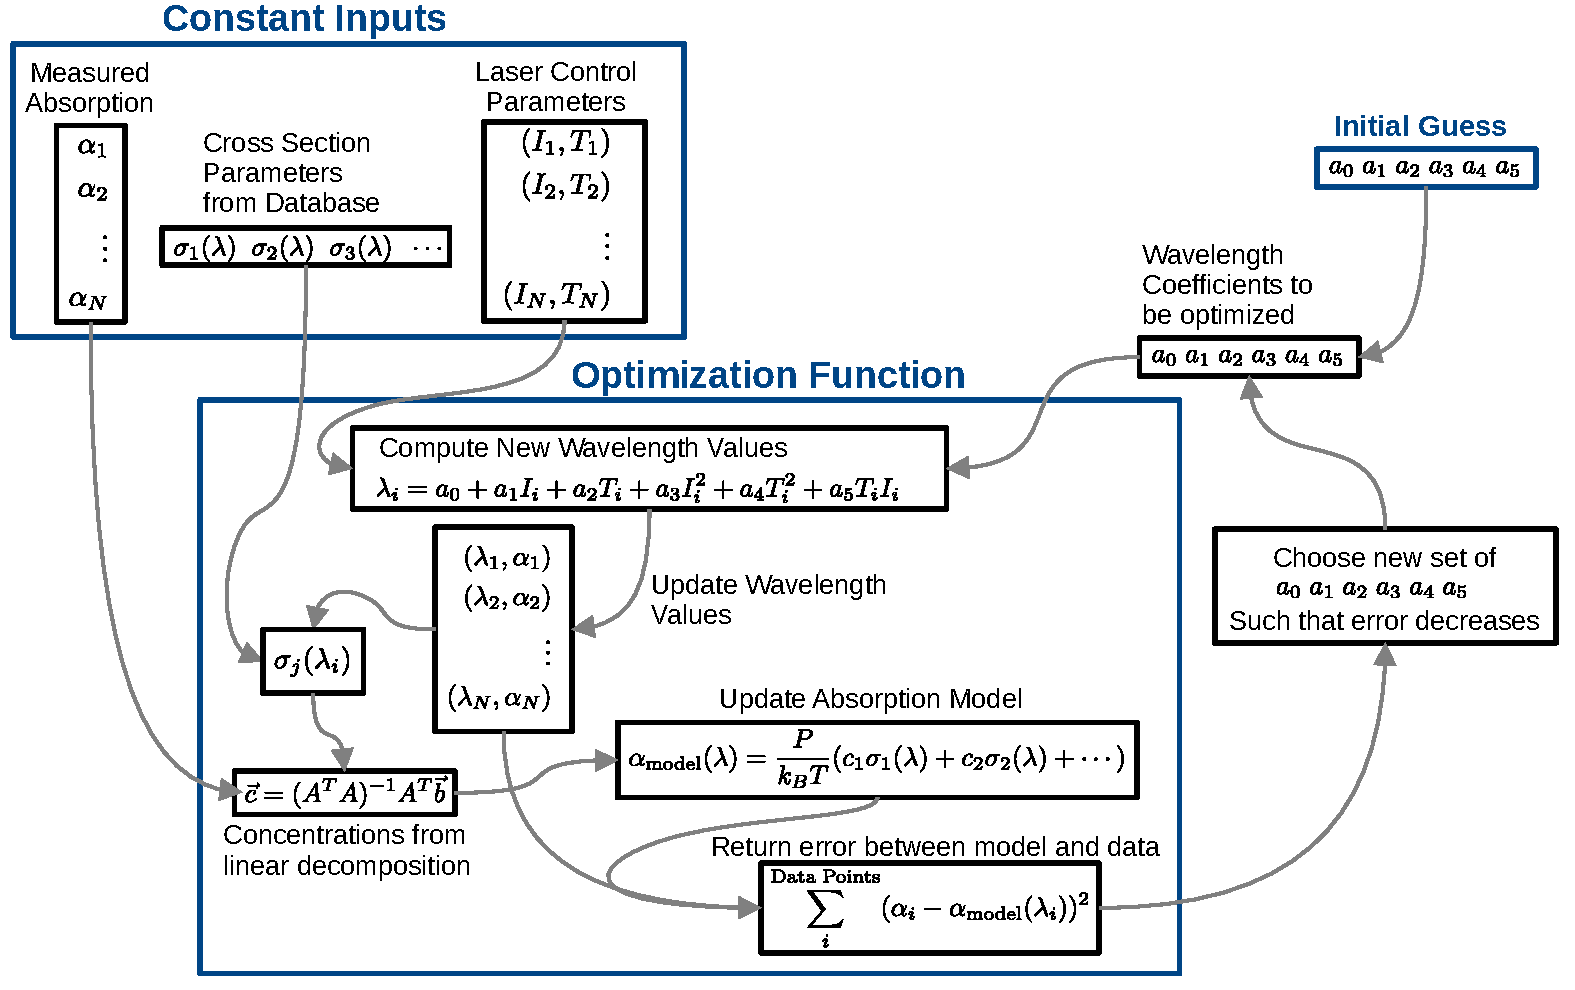
\includegraphics[width=1.0\linewidth]{diagrams/det_algorithmFlowchart}
		\caption{Algorithm flowchart shown for determination of the six detuning coefficients $a_{0\ldots 5}$ in \ref{det_quadratic}. Starting with an initial guess for these coefficients, a set of wavelength values $\lambda_i(I_i, T_i)$ are computed from the current and temperature values $I_i$ and $T_i$ measured during the scan. These are used to compute the optical cross section values of the various species at these computed wavelengths. These cross section values are entered into (\ref{leastSquares}) to obtain the concentration values of the various gas species, which gives a spectrum of best fit constructed as a linear combination of absorption cross sections. The squared residuals between the measured absorption values and those predicted by the curve of best fit are summed to give a single scalar value. A new set of detuning coefficients is then chosen to decrease the value of this scalar. The process of choosing new $a_{0\ldots 5}$ is handled by a nonlinear optimization procedure, which was the Nelder-Mead procedure in this work.}
		\label{fig:det_algorithmflowchart}
	\end{figure}
	
	\section{Demonstration of Algorithm Performance}
	In this section, we give direct measurements of the algorithm's performance in regard to the detuning recovery ability, and the concentration extraction.
	
	\subsection{Evaluation of Wavelength Recovery Ability}
	
	\begin{figure}[H]
		\centering
		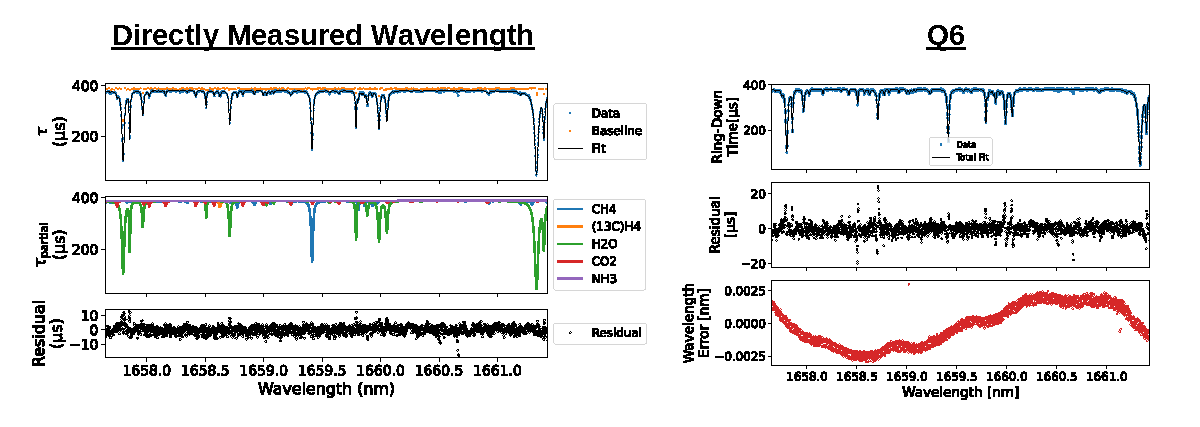
\includegraphics[width=1.0\linewidth]{diagrams/det_algorithmPerf_residual_L2}
		\caption{Performance of the detuning inference algorithm on a breath sample measured with Laser 2. On the left is a spectrum containing approximately 4,000 points collected with CRDS having the wavelength axis calibrated by direct measurement. Shown in the middle and right plots is result of discarding this wavelength information and using the laser parameters $I$ and $T$, corresponding to the injection current and temperature of a DFB laser diode, to infer the laser tuning behavior.}
		\label{fig:det_algorithm_perf_residual_L2}
	\end{figure}
	
	\begin{figure}[H]
		\centering
		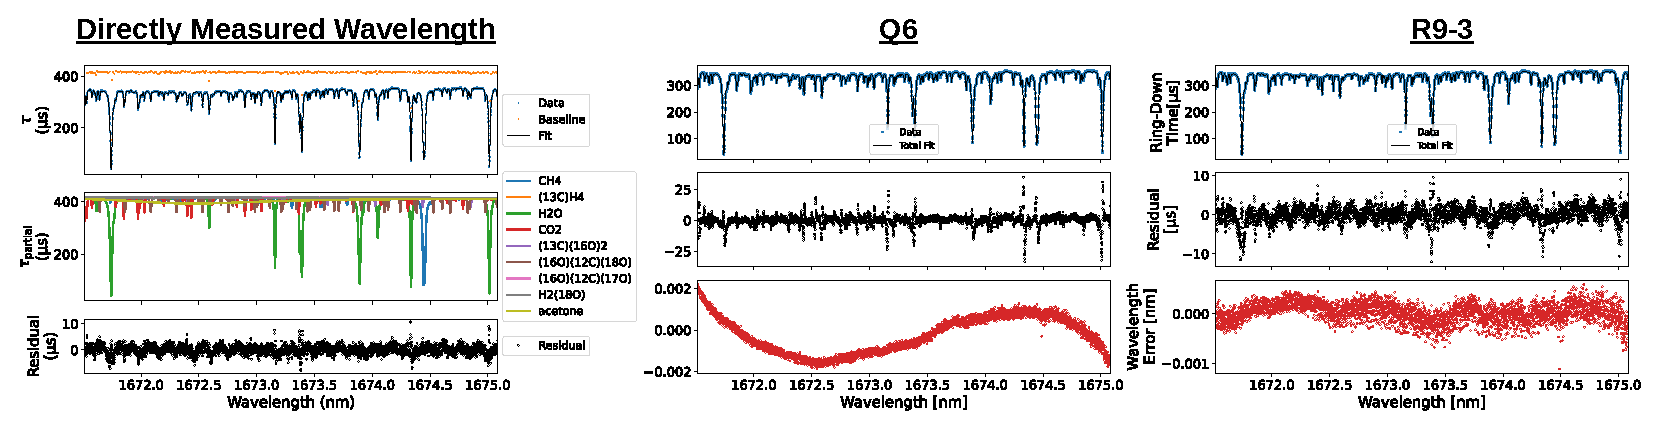
\includegraphics[width=1.0\linewidth]{diagrams/det_algorithmPerf_residual}
		\caption{Performance of the detuning inference algorithm on a breath sample measured with Laser 3. On the left is a spectrum containing approximately 4,000 points collected with CRDS having the wavelength axis calibrated by direct measurement. Shown in the middle and right plots is result of discarding this wavelength information and using the laser parameters $I$ and $T$, corresponding to the injection current and temperature of a DFB laser diode, to infer the laser tuning behavior. We compare here the effect of using two different models, both having six parameters. It can be seen that the performance of the R9-3 model is far superior to that of the Q6 model, having much lower deviation in the predicted wavelength from the recorded value and better residual structure. A comparison of the gas concentration values extracted from each calibration method is shown in Table \ref{table:det_conc_table}.}
		\label{fig:det_algorithmperf_residual_L3}
	\end{figure}
	
	\begin{figure}[H]
		\centering
		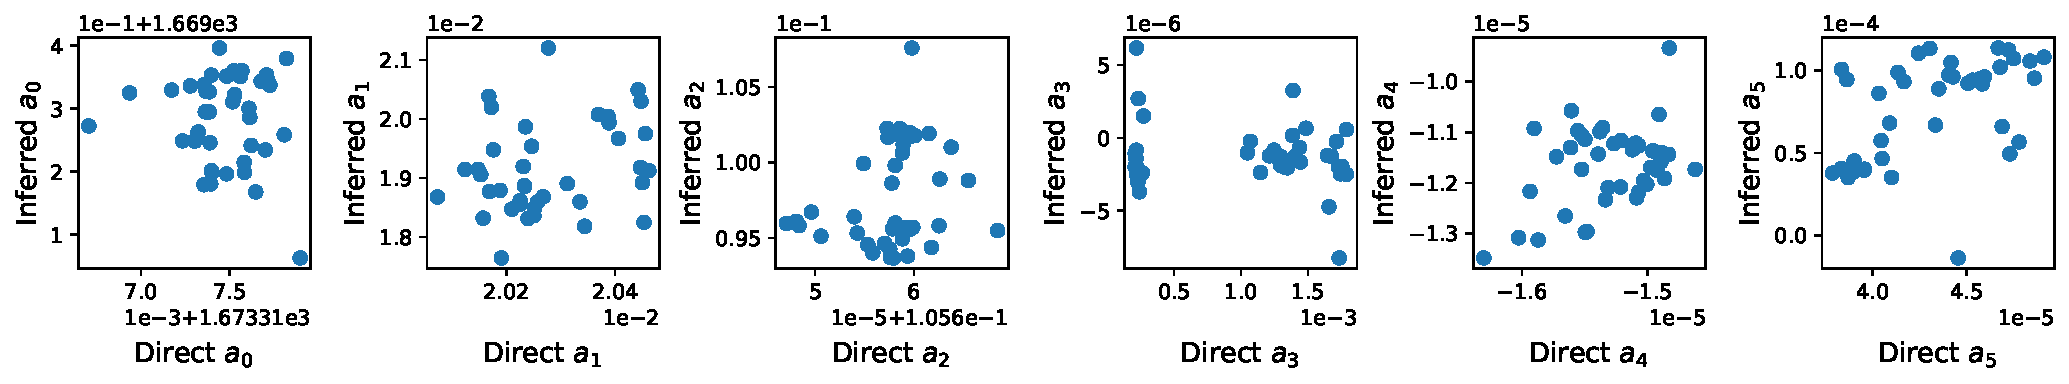
\includegraphics[width=1\linewidth]{diagrams/det_coeffCompare_Q6}
		\caption{Comparison of the Q6 detuning coefficients obtained by directly measuring the wavelength values at each point in the spectrum scans against those recovered by the proposed algorithm.}
		\label{fig:det_coeffCompare_Q6}
	\end{figure}
	
	\begin{figure}[H]
		\centering
		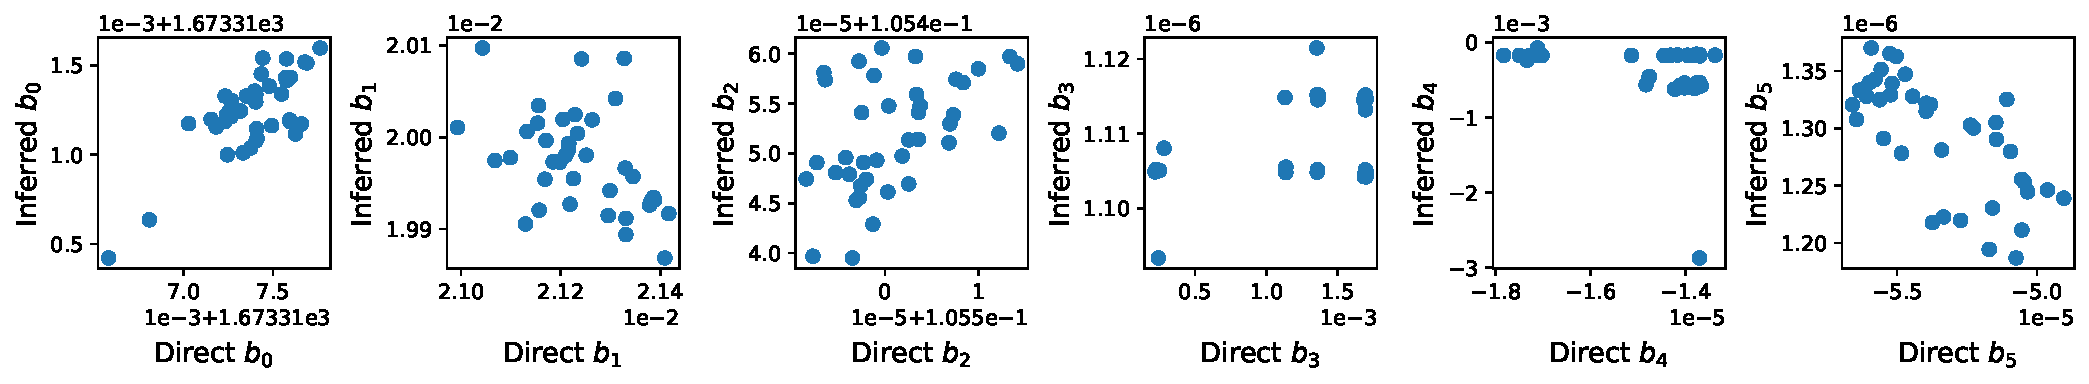
\includegraphics[width=1\linewidth]{diagrams/det_coeffCompare_R9-3}
		\caption{Comparison of the R9-3 detuning coefficients obtained by directly measuring the wavelength values at each point in the spectrum scans against those recovered by the proposed algorithm.}
		\label{fig:det_coeffCompare_R9-3}
	\end{figure}
	
	\subsection{Concentration Recovery}
	
	\begin{figure}[H]
		\centering
		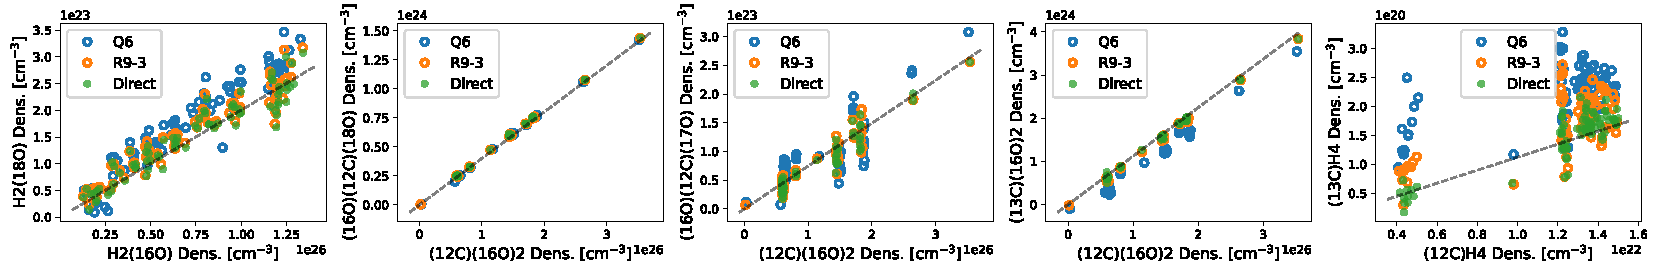
\includegraphics[width=1.0\linewidth]{diagrams/det_isoRatio_las1}
		\caption{Isotope ratios for five different isotopologues measured within the tuning range of Laser 3. Plotted are ensembles of concentrations recovered from spectrum scans. For each scan, the data is analyzed using the directly measured wavelengths (shown with the Direct points in green). For the other points shown, the wavelength information was discarded, and the proposed wavelength detuning recovery algorithm was used. The performance of two different wavelength detuning models is shown. When the R9-3 model is used with the procedure (shown with the orange points), much better agreement with the accepted value for these isotope ratios (shown with the dashed black line) is obtained than with the Q6 model (shown with the blue points).}
		\label{fig:detisoratiolas1}
	\end{figure}
	
	\begin{table}[H] 
		\begin{center}
			\caption{For the spectrum data shown in Fig. \ref{fig:det_algorithmperf_residual_L3}, the recovered concentrations of each species is compared using different methods of wavelength calibration. For the assumption of the Q6 and R9-3 detuning models, the proposed algorithm returns values for the concentrations which agree well with the fit of the same spectrum having its wavelength axis directly measured.}\label{table:det_conc_table}
			\setlength{\extrarowheight}{3pt} % Space for exponentials
			\begin{NiceTabular}{|l|l|l|l|}
				\hline
				\rowcolor{gray!40} Molecule & Q6 Conc. [ppm] & R9-3 Conc. [ppm] & Direct Conc. [ppm] \\
				\hline
				(12C)H4 & 4.261 & 4.268 & 4.298 \\
				\hline
				(13C)H4 & 0.07868 & 0.0724 & 0.05199 \\
				\hline
				H2(16O) & 15220 & 15720 & 15660 \\
				\hline
				(12C)(16O)2 & 19770 & 19310 & 19130 \\
				\hline
				(13C)(16O)2 & 104.2 & 194.8 & 200.8 \\
				\hline
				(16O)(12C)(18O) & 78.95 & 79.56 & 79.62 \\
				\hline
				(16O)(12C)(17O) & 24.32 & 13.52 & 13.69 \\
				\hline
				H2(18O) & 45.99 & 40.25 & 38.07 \\
				\hline
				(14N)H3 & 0.01897 & 0.04021 & 0.01631 \\
				\hline
			\end{NiceTabular}
		\end{center}
	\end{table}
	
	
	
	\chapter{CAVITY ENHANCED ABSORPTION SPECTROSCOPY WITH MULTIPLEXED DETECTION} \label{chap:comb_ceas}
	
	\section{Frequency Combs}
	Optical frequency combs were already discussed in Sec. \ref{sec:wl_combs}, where they were discussed as a tool for the measurement of optical frequencies. In this section, we consider properties of combs that are useful as direct probes of broadband absorption.
	
	Optical frequency combs, generated via the carrier-envelope phase stabilization of passively mode-locked lasers, offer unparalleled advantages for sensitive spectroscopic detection \cite{book_ceas}. The combination of broad optical bandwidth, being composed of many discrete optical frequencies stabilized to radio frequency references, makes the frequency comb a powerful tool for precision spectroscopy \cite{book_yeCundifff_combs}. Combined with techniques of optical path amplification provided by a high finesse cavity, very sensitive instruments can be constructed which combine the precision of an optical frequency comb with sensitivity on par with cavity ring-down spectroscopy.
	
	A frequency comb is defined by a series of discrete frequencies $\nu_n$, determined by the repetition rate $f_{\text{rep}}$ and the carrier-envelope offset frequency $f_{\text{CEO}}$
	\begin{equation} \label{comb_modes}
		\nu^\mathrm{comb}_n = f_{\text{CEO}} + n f_{\text{rep}}
	\end{equation}
	for integer values of $n$. This structure offers a dual advantage: the broadband nature allows for the simultaneous interrogation of multiple molecular transitions, while the fixed spacing enables unambiguous absolute frequency calibration.
	
	In Sec. \ref{sec:cav_transmission}, we established that an optical cavity, in the absence of a dispersive medium, produces transmission maxima that are also evenly spaced in frequency. The most efficient coupling of a frequency comb to such a cavity requires precise matching of these two periodicities. Taking name inspiration from the Vernier scale used on mechanical measurement devices, Vernier spectroscopy exploits the intentional mismatch of these two frequency scales to give an output which can be tailored to simplify their simultaneous detection.
	
	\section{Vernier Spectroscopy}
	
	Vernier spectroscopy utilizes the optical mode structure of a high-finesse cavity to provide both extended optical path length and high spectral resolution. By using the cavity as a spectral filter that is periodic in the frequency domain, a Moiré pattern is created against the repeating comb modes. This filtering yields an effective transmission spacing, $f_{\text{Vernier}}$, which can be significantly larger than the fundamental repetition rate $f_{\text{rep}}$ by a controllable amount. This expansion of the spectral scale allows relatively simple spectrometers--such as those employing diffraction gratings and broadband detectors--to resolve spectral features that would otherwise be obscured by the dense comb structure.
	
	\begin{figure}[H]
		\centering
		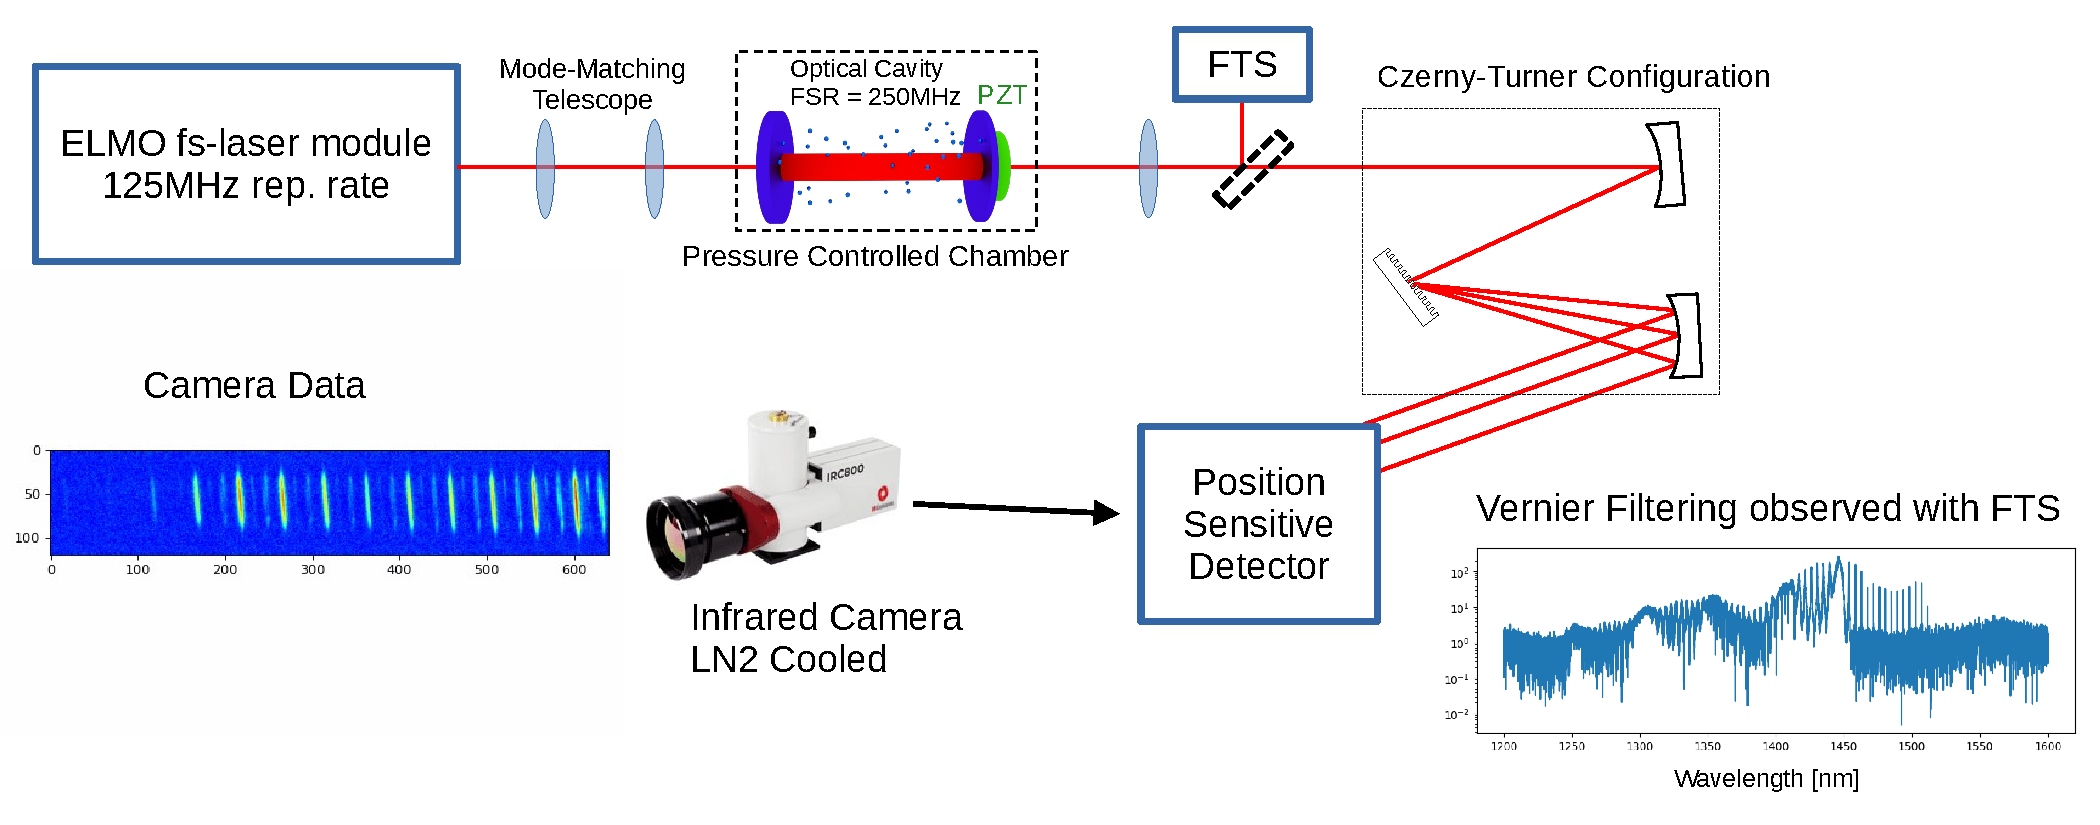
\includegraphics[width=1.0\linewidth]{diagrams/vernier_setup}
		\caption{Setup used to perform Vernier spectroscopy. A compact frequency comb source (Menlo Systems ELMO) operating at 125MHz repetition rate is mode-matched to a high finesse optical cavity. One of the cavity mirrors has an electronically adjustable position using a translation stage (not shown) and a piezoelectric actuator (PZT). The cavity output is optionally sent to a Fourier transform spectrometer (FTS) using a flip mirror. At the other toggle position of the mirror, the beam is sent to a Czerny-Turner spectrometer which spectrally disperses the light, mapping the spectrum onto a well-defined position. This dispersed light is collected by a liquid nitrogen cooled infrared camera which reads the optical spectrum.}
		\label{fig:vernier_setup}
	\end{figure}
	
	
	The complexity of this coupling arises because, unlike a CW laser which only requires matching a single resonance, a comb requires managing the overlap of two periodic structures. Furthermore, dispersion--arising from mirror coatings and the gaseous medium within the cavity--breaks the perfect periodicity of both the comb and the cavity modes. This dispersion imposes additional constraints on the carrier envelope offset frequency of the comb. Vernier filtering is the result of intentionally mismatching the comb repetition rate to the free spectral range of the cavity to form a moiré pattern of transmissions that are much more widely spaced than either the comb modes or the cavity free spectral range.
	
	From Equation (\ref{cav_airy}) in Sec. \ref{sec:cav_transmission}, we found that the intensity transfer function for an optical cavity can be written as the Airy transmission
	\begin{equation}\label{vernier_airy}
		H(\nu) = \frac{H_\text{max}}{1 + \left(\frac{2F}{\pi} \right) ^2 \sin ^2 \left[\phi(\nu)/2\right]}
	\end{equation}
	where $F=\pi \sqrt{R}/(1-R)$ is the finesse of the cavity and $H_\text{max} = T^2/(1-R)^2$ is the maximum transmission. The phase $\phi(\nu)$ represents the round-trip phase accumulation
	\begin{equation}
		\phi(\nu) = 2\pi \nu \frac{L}{c} - \phi_0
	\end{equation}
	For $F\gg1$, the Airy transmission gives sharp peaks, which are periodic in optical frequency with spacing $\mathrm{FSR} = c/n_rL$, where $L$ is the round-trip length of the cavity. A comb interating with this transmission envelope creates "Vernier resonances" at a frequency spacing $f_{\text{Vernier}} = (f_{\text{rep}} \cdot \text{FSR}) / |\text{FSR} - f_{\text{rep}}|$, providing the basis for multiplexed, high-throughput absorption spectroscopy. For the moment, we will assume that the refractive index is unity $n_r=1$, corresponding to vacuum and zero dispersion.
	
	\subsection{High Finesse Limit -- Single Comb Mode Transmission}
	
	Vernier filtering \cite{vernier_gohle} takes place when every $n^\mathrm{th}$ frequency comb mode is resonant with every $m^\mathrm{th}$ cavity resonance ($f_\mathrm{Vernier} = nf_\mathrm{rep} = m \mathrm{FSR}$). This condition is depicted for $(m,n) = (9, 10)$ in Fig. \ref{fig:vernier_ratiodiagram}, where it can be seen that if we choose to set $n = m + 1$, then we create the condition where every $m^\mathrm{th}$ cavity mode coincides with the $n^\mathrm{th}$ comb mode, creating an effective spacing between the transmitted modes which is $m \mathrm{FSR}$. That is, by satisfying the condition
	\begin{equation} \label{vernier_ratio_definition}
		\frac{f_\mathrm{rep}}{\mathrm{FSR}} = \frac{m}{m+1}
	\end{equation}
	the effective spacing of the transmitted comb modes, $f_\mathrm{Vernier}$, is the magnified FSR of the cavity
	\begin{equation}
		f_\mathrm{Vernier} = m \mathrm{FSR}
	\end{equation}
	The particular example for $m=9$ is shown in Fig. \ref{fig:vernier_ratiodiagram}.
	
	
	%The Vernier condition (\ref{vernier_ratio_definition}) necessitates that the frequency-dependent round trip phase accumulation $\phi(\nu)$ has maxima where $\phi(\nu^\mathrm{comb}_n) = n' \cdot 2\pi$ where $n'$ is some integer.
	
	A perfect matching of the comb teeth and cavity resonance spacings would ($m=n$) require the condition that each comb line lands on maxima of (\ref{vernier_airy})
	\begin{equation}
		\phi(\nu^\mathrm{comb}_n) = 2\pi (n f_\text{rep} + f_\text{ceo}) L_\text{rep}/c - \phi_0 =  n \cdot 2 \pi
	\end{equation}
	For a comb of a particular repetition rate, resonance we requires that set the cavity length to be $L_\text{rep} = c/f_\text{rep}$, and the laser carrier envelope offset to be $f_\text{ceo} = (\phi_0/2\pi)\cdot f_\text{rep}$. This corresponds to the case where the comb teeth are landing on the maxima of the Airy function in (\ref{cav_airy}).
	
	The formation of the Vernier ratio (\ref{vernier_ratio_definition}) can be performed by finding the perfect matching length $L_\mathrm{rep}$ corresponding to $m=n$, usually found by noting that the transmitted power is sharply maximized in this region, and then displacing away from this value by a known distance $\Delta L$. Experimentally, this removes the necessity to measure the cavity mirror spacings with absolute precision, since $L_\mathrm{rep}$ is effectively calibrated to the comb repetition rate.
	
	However, when the matching condition of Eq. (\ref{vernier_ratio_definition}) is fulfilled, the cavity gives an output similar to that of a comb having a repetition rate of $(m+1)$ times the original repetition rate, as can be seen from Fig. \ref{fig:vernier_ratiodiagram}, where the completely transmitted comb modes are marked with gray circles. For a high-finesse cavity, we can assume that only one comb mode is transmitted in the vicinity of each cavity resonance, and the condition of Eq. (\ref{vernier_ratio_definition}) holds to desribe the effective spacing of the transmitted modes. The transmission function for a comb coupled to a cavity having a lower finesse has been explored elsewhere \cite{vernier_continuous_filtering}.
	
	\begin{figure}[H]
		\centering
		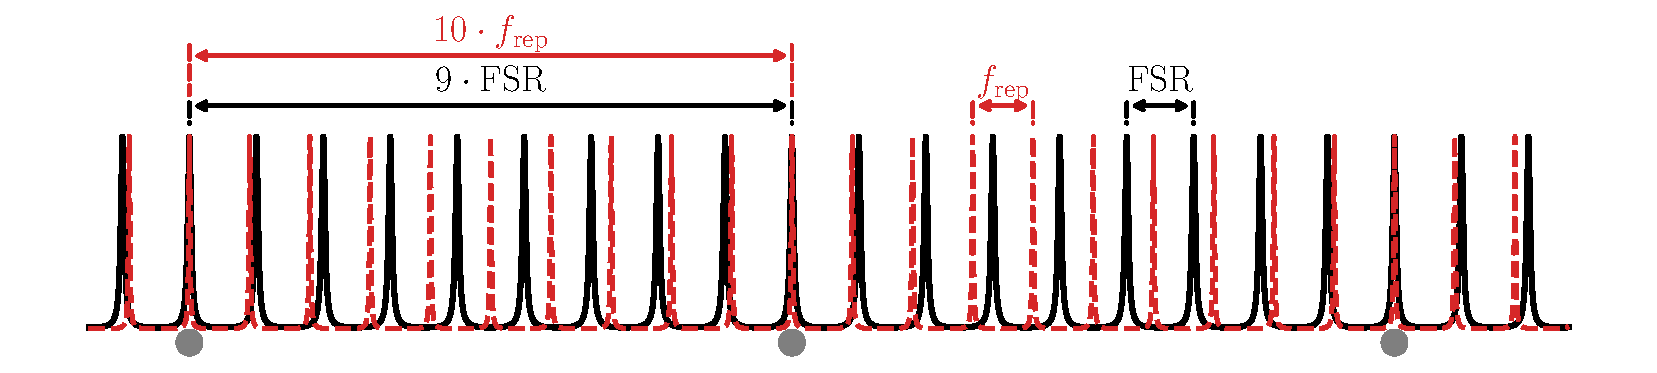
\includegraphics[width=1.0\linewidth]{diagrams/vernier_ratioDiagram}
		\caption{Vernier filtering for $m=9$. The periodic cavity transmissions and comb modes form two overlapping scales. By appropriately choosing the spacing, we can create a Moiré pattern of resonances caused by the periodic overlap of these scales (seen as the gray dots, where the peaks overlap). This Moiré pattern functions as a Vernier scale if the ratios are of the form $m/(m+1)$.}
		\label{fig:vernier_ratiodiagram}
	\end{figure}
	
	\subsubsection{Extration of Absorption}
	
	In the discrete limit of Vernier spectroscopy, we can apply the discussion of Sec. \ref{sec:cav_laser_sweep} for a laser sweeping across a cavity resonance. While the exact structure of the time domain signal corresponding to a single comb line sweeping over a cavity resonance (or vice versa) is a complicated mixture of beating and exponential decay, it was found that the integral of this signal was proportional to the ring-down time of the cavity. We can use this observation for analyzing the response of a slow detector in order to obtain a measure of the intra-cavity absorption.
	
	The calculation of intra-cavity absorption can be conducted as follows. Assuming that the laser spectrum remains constant between the measurement of an empty cavity and a cavity containing the target gas, measuring both $\tau$ and $\tau_0$ is sufficient to determine the intracavity optical absorption $\alpha$. We assume that the detector lacks the temporal resolution to resolve the ring-down event in real time, and instead captures an integration of the signal. For the exponentially decaying signal characteristic of cavity ring-down, this integration yields a value proportional to the ring-down time, indicated in Sec. \ref{sec:cav_laser_sweep}. By calculating the ratio between the measurements of the cavity with and without the absorber gas, one can obtain the ratio $\tau/\tau_0$. The optical absorption of the intracavity gas can then be determined from
	\begin{equation}
		\alpha = \frac{1-R}{L}\left(\frac{\tau_0}{\tau} -1\right)
	\end{equation}
	
	Because the integrated intensity of the swept comb mode is proportional to $\tau$, the ratio $\tau/\tau_0$ can be reliably replaced by the ratio of the observed slow-detector signals. It should be noted that, unlike CRDS, the determination of the absorption coefficient is not calibration-free, as it depends explicitly on the values of the mirror reflectivity and the cavity round-trip length $L$. Only the observation of the detailed ring-down transient would permit a truly calibration-free approach.
	
	\subsubsection{Calibration of the Frequency Axis and the Retrieval of All Comb Modes}
	Although most comb modes have been filtered from the transmission signal, the missing modes can still be measured by either scanning the cavity length or the comb repetition rate. This approach allows for the collection of signals in an interleaved fashion on a spectrally resolved detector, which effectively bypasses the resolution limits of said detector. By choosing an $m$ value that is sufficiently high, the spacings between the transmitted vernier orders can be made large enough so that minimal requirements are imposed on the detector resolution.
	
	In the discrete Vernier regime, clearly defined individual comb-cavette resonance events can be observed on a spectrally resolving detector as the system is scanned. By counting these resonance events while either the cavity or the comb is scanned, one can attribute the frequency spacing of subsequent resonant events to the underlying spacing of the comb modes. Such a scheme for interleaved spectrum retrieval is demonstrated in Fig. \ref{fig:vernier_discretecounting}, where the time axis is depicted as a streak-camera image and the spectrum is unwrapped using fixed absorption features, which serve as markers for the frequency calibration offset. In this manner, we can uniquely determine $m$, the frequency scale, and the frequency offset.
	
	\begin{figure}[H]
		\centering
		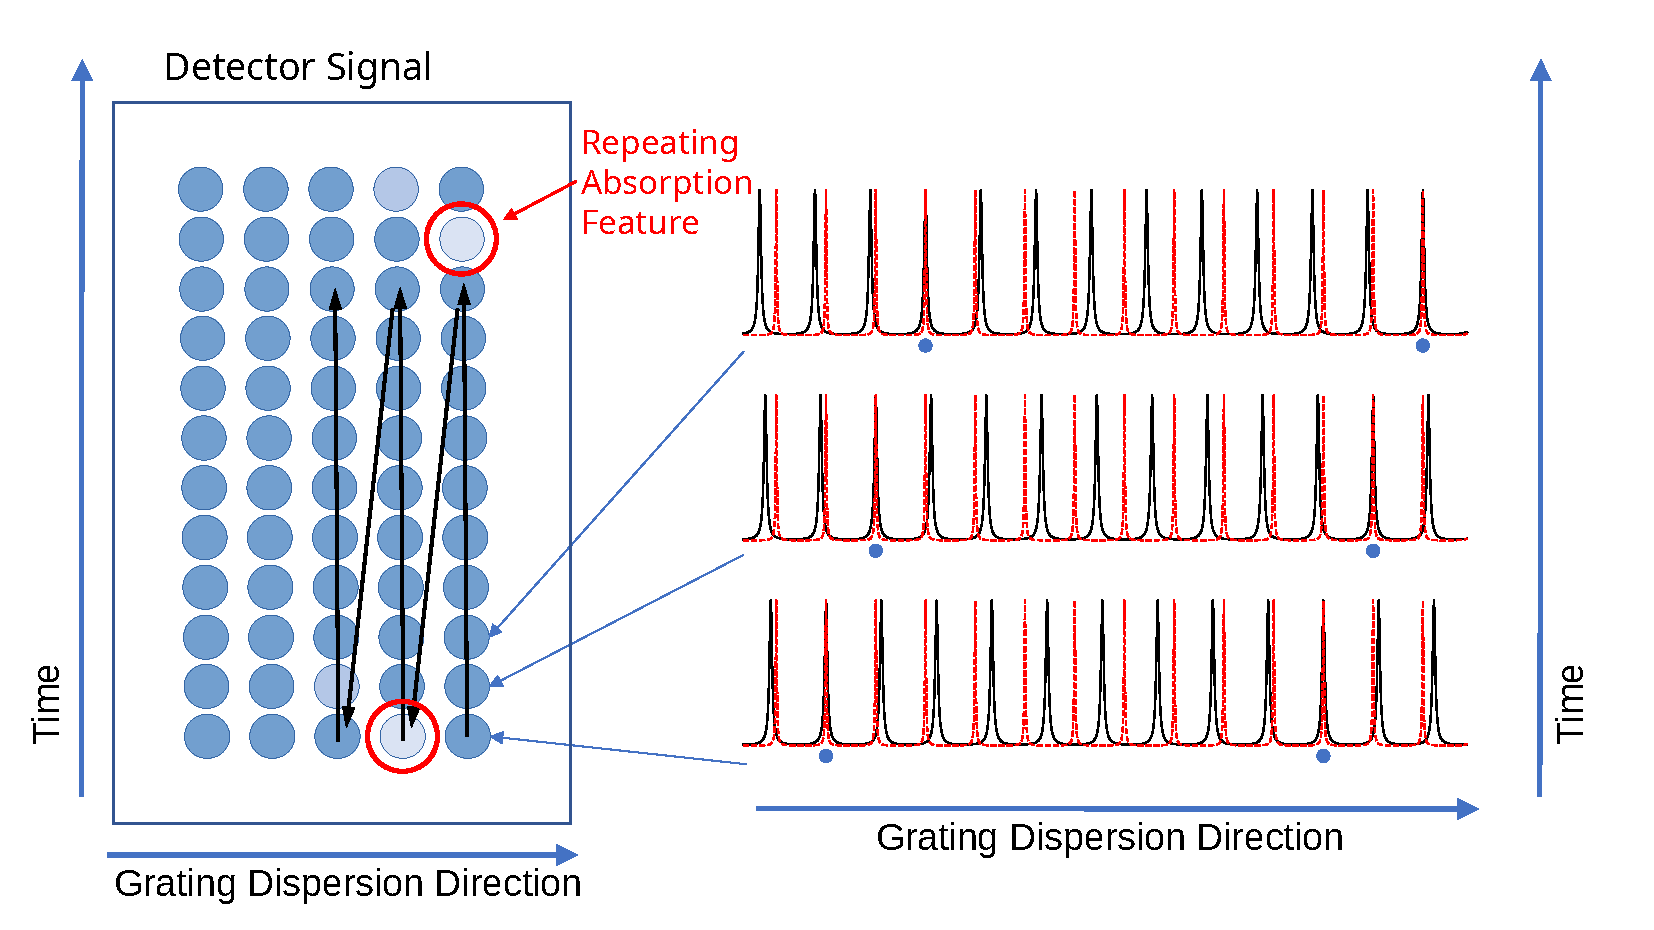
\includegraphics[width=0.8\linewidth]{diagrams/vernier_discreteCounting}
		\caption{The spectrally resolved detector signal is depicted as a function of time, where each spot in the detector signal represents a discrete resonance event. For each event, the slow-detector signal provides an output amplitude proportional to the ring-down time, which is represented by the spot color, and a position that reflects the frequency of the transmitted light. The vertical axis of this image corresponds to the time axis, as it is displayed in the manner of a streak camera trace. The process of reconstructing the interleaved spectrum is shown with the black arrows.}
		\label{fig:vernier_discretecounting}
	\end{figure}
	
	
	%Another version of this formula appears when the ratio $\tau_0/\tau$ is formed from the exact expressions (\ref{tau_exact}) and (\ref{tau_vac_exact}).
	
	\subsection{Continuous Vernier Regime}
	The previous discussion assumed that comb modes which did not perfectly coincide with cavity transmission maxima were completely filtered out. Here we remove this assumption and proceed to a regime where these other modes have a non-negligible contribution to the cavity output.
	
	For a sufficiently high finesse cavity, if its length is scanned around a value which corresponds to particular choice of $m$ in the Vernier definition \ref{vernier_ratio_definition}, the cavity transmission is almost completely extinguished until the next integer matching condition is fulfilled, creating discrete resonance events. When the finesse value is diminished, these discrete resonance events smear together into an oscillatory continuum.
	
	In this continuous regime \cite{vernier_continuous_filtering}, we may upgrade the integer $m$ to a continuous "magnification factor" $\mathcal{M}(L)$ which is dependent on the cavity length. From the definition (\ref{vernier_ratio_definition}), we may write this as
	\begin{equation}
		\mathcal{M}(L) = \frac{f_\mathrm{rep}}{\mathrm{FSR}(L) - f_\mathrm{rep}} = \frac{-L}{\Delta L } \approxeq \frac{-L_\mathrm{rep}}{\Delta L}
	\end{equation}
	where $\Delta L = L - L_\mathrm{rep}$ is the displacement away from the perfect matching length $L_\mathrm{rep} = c/f_\mathrm{rep}$. With this definition, the two parameters of the emerging Vernier comb, along with the FWHM of the transmitted modes, are \cite{vernier_continuous_filtering}
	\begin{align}
		f_\mathrm{Vernier} &= \mathcal{M}\cdot \mathrm{FSR} \\
		f_\mathrm{V, 0} &= \mathcal{M} \cdot \delta f_\mathrm{CEO}\\
		\Gamma_\mathrm{V} &= \mathcal{M}\cdot \Gamma_\mathrm{Cav} = \frac{\mathcal{M}}{F} \cdot \mathrm{FSR}
	\end{align}
	Above, $\delta f_\mathrm{CEO} = ((\frac{\phi_0}{2\pi}) - 1)\cdot f_\text{rep}$, is the difference between the comb's carrier envelope offset frequency and the perfect matching offset given by the round-trip phase shift $\phi_0$.
	
	A critical feature of this technique occurs when the cavity finesse is relatively low, where the width of the effective Vernier envelope $\Gamma_\mathrm{V}$ is large enough to encompass multiple comb teeth. For a spectrometer which lacks the optical frequency resolution to resolve the individual $f_{\text{rep}}$ teeth, it "sees" a group of teeth as a single spectral feature. The amplitude of this spectral feature looses dependence on the comb parameters, greatly relaxing the comb stability requirements.
	
	\begin{figure}[H]
		\centering
		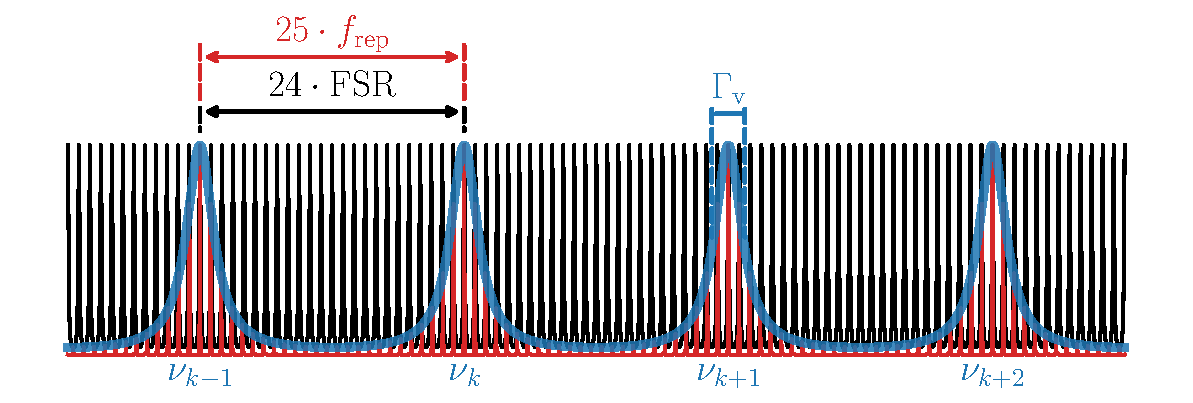
\includegraphics[width=1.0\linewidth]{diagrams/vernier_continuousDiagram}
		\caption{Continuous Vernier regime, where multiple comb modes are transmitted every $k^\mathrm{th}$ Vernier order $\nu_k$. Depicted here is the magnification factor $\mathcal{M}=24$. The comb modes are shown in red with spacing $f_\mathrm{rep}$ with amplitudes corresponding to the transmitted intensity due to comb filtering. The steady state transmission amplitude of the cavity is shown black. The Moiré patten of resonances also follows an Airy transmission envelope, which is shown in blue. The effective width $\Gamma_\mathrm{V}$ of these Vernier orders is shown as the FWHM of the envelope.}
		\label{fig:verniercontinuousdiagram}
	\end{figure}
	
%	\subsection{Regimes for Spectrally Resolved of the Transmitted Light}
%	
%	\hl{!!!!!!!!!!!!!!!!!!!!!!!!!!!!!!!!!!}
%	
%	The ability to extract spectroscopic information from the Vernier-filtered signal depends fundamentally on the relationship between the detector’s bandwidth and the characteristic timescales of the cavity dynamics. While the Vernier effect provides an electronic frequency ruler in the $f$-domain, the physical information resides in the modulation of the optical field as it traverses the cavity resonances in the $\nu$-domain. Depending on the acquisition hardware used, the detected signal can be interpreted through two distinct temporal regimes. In the first regime, where the detector bandwidth is significantly lower than the reciprocal ring-down time of the cavity, the photodetector acts as a continuous integrator for the transient interactions with the cavity; it effectively smooths over the resulting oscillations to provide a time-averaged power spectrum, capturing only the steady-state response.
%	
%	In the second, more high-resolution regime, the detector bandwidth is sufficient to resolve the transient dynamics of the light intensity. Here, the measurement captures the rapid buildup and subsequent ring-down transients of the cavity intensity as the comb modes sweep through the resonance, considered as a superposition of the monochromatic transients investigated in Ch. \ref{chap:cav_dynamics}. In this regime, the detector does not merely record a static absorption magnitude, but rather samples the time-evolution of the cavity's response to the modulated input field. This distinction is critical: while the former regime is suitable for traditional broadband absorption measurements, the latter enables the high-speed, transient-based sensing required for advanced applications such as rapid-scan CRDS and real-time molecular monitoring [CITE].
%	
%	The detection of this transmitted signal can be modeled through the lens of a general spectrometer characterized by its resolution kernels in both frequency and time. Let the transmitted optical field be $\mathcal{E}(\nu, t)$. A physical detector performs a measurement defined by the convolution of the signal with a multidimensional window function $R(\nu, t; \delta\nu, \delta t)$:
%	\begin{equation}
%		S(\bar{\nu}, \bar{t}) = \iint \mathcal{E}(\nu, t) \cdot R(\nu - \bar{\nu}, t - \bar{t}; \delta\nu, \delta t) \, d\nu \, dt
%	\end{equation}
%	Here, $\delta\nu$ represents the spectral resolving power of the spectrometer (the width of the frequency-domain filter), and $\delta t$ represents the temporal resolution (the uncertainty in arrival time or modulation frequency). 
%	
%	In the context of Vernier spectroscopy (and broadband CEAS in general), the experimentalist is faced with a fundamental trade-off rooted in the time-frequency uncertainty principle. There exist two mutually exclusive approaches to performing "calibration-free" absorption measurements, and a single spectrometer cannot achieve unbounded precision in both domains simultaneously. The first approach focuses on spectral resolution, where the detector bandwidth is extremely narrow. In this regime, the measurement effectively integrates over many successive cavity transients (or pulses), accumulating signal to resolve the precise width of the Airy resonance as a function of optical frequency. This maximizes $\delta\nu$ at the expense of $\delta t$, essentially treating the spectrometer as a high-resolution frequency-domain filter.
%	
%	The second approach focuses on temporal resolution, where the detector bandwidth is large enough to capture the individual, transient decay events of the cavity intensity. In this regime, the measurement captures the ring-down time $\tau$ (or its modulation) as a function of optical frequency. Here, $\delta t$ is minimized to resolve the rapid decay dynamics, but the spectral resolution $\delta\nu$ is limited by the integration of these transient pulses over the detector's response window. Ultimately, the spectrometer must be optimized for one of these two extremes: either capturing the precise spectral fingerprint of a steady-state resonance or resolving the temporal signatures of the cavity's impulse response.
	
	\subsection{Impact of Molecular Absorption and Dispersion on the Vernier Pattern}
	
	The ideal Vernier pattern described in the previous sections assumes a vacuum-filled cavity with constant reflectivity and zero dispersion. However, the fundamental purpose of this architecture is to perform trace gas analysis, which necessitates the introduction of a molecular medium into the cavity. The presence of an absorbing species introduces two simultaneous perturbations to the cavity transfer function: an increase in round-trip loss (attenuation) and a frequency-dependent phase shift (dispersion).
	
	\subsubsection{Attenuation and the Reduction of Peak Transmittance}
	
	The primary signal of interest in Cavity Enhanced Absorption Spectroscopy (CEAS) is the reduction in light intensity due to molecular absorption. As established in Sec. \ref{sec:cav_td_response}, an absorbing medium with a frequency-dependent absorption coefficient $\alpha(\nu)$ modifies the effective reflectivity of the cavity. For a single pass through a gas of length $L$, the transmission is attenuated by a factor of $e^{-\alpha(\nu) L}$. Within the context of the high-finesse cavity, this loss is accumulated over many round trips, effectively modifying the reflectivity $R$ to a frequency-dependent value $R(\nu)$:
	\begin{equation} \label{eq:eff_reflectivity}
		R(\nu) = R_{\text{vac}} \exp\left( -\alpha(\nu) L \right)
	\end{equation}
	where $R_{\text{vac}}$ is the reflectivity of the mirrors in vacuum. From (\ref{cav_E-sum}), this gives the transfer function for the electric field \cite{vernier_continuous_filtering} as
	\begin{equation}
		h(\nu) = \frac{T}{1 - R \cdot \exp\left[-\frac{1}{2}\alpha(\nu)L\right]\cdot \exp\left[- i \Phi(\nu)\right]}
	\end{equation}
	with modified round trip phase
	\begin{equation}
		\Phi(\nu) = \frac{2\pi \nu}{c} \left( L_\mathrm{rep} + \Delta L - \delta n(\nu) \right) - \phi_0
	\end{equation}
	containing the term $\phi_\mathrm{abs}(\nu) = (2\pi\nu/c)\delta n(\nu) L$ arising from optical index variation $\delta n(\nu)$. This refractive index variation is itself related to the absorption coefficient through the Kramers-Kronig relations.
	
	The cavity transfer function for the transmitted optical power, expressed at the comb frequencies in the vicinity of the $k^\mathrm{th}$ Vernier order (see Fig. \ref{fig:verniercontinuousdiagram}) as
	\begin{equation}
		H(\nu_n^\mathrm{comb}) = \frac{H_\mathrm{max}}{\left(1 + \frac{F}{2\pi}\alpha\left(\nu_n^\mathrm{comb} \right)L\right)^2} \frac{1}{1 + \left[\frac{\nu_n^\mathrm{comb} - \nu_k^\mathrm{V} - \delta \nu_c(\nu_n^\mathrm{comb}) L/\Delta L}{\frac{1}{2}\left(\Gamma_c + \delta \Gamma_c(\nu_n^\mathrm{comb})\right) L/\Delta L}\right]^2}
	\end{equation}
	where $\delta\nu_c = \frac{\phi_\mathrm{abs}}{2\pi}\frac{c}{L} = \nu \cdot\delta n$ is the shift of the resonance frequency due to the absorbing species and $\delta\Gamma_c(\nu) = \frac{c}{2\pi}\alpha(\nu)$ is the increased cavity resonance linewidth. This can be written in terms of the magnification factor $\mathcal{M}$ to give the Vernier response function \cite{vernier_continuous_filtering}
	\begin{equation}
		H_\mathrm{V}(\nu) =
		\frac{H_\mathrm{max}}{\left(1 + \frac{F}{2\pi}\alpha\left(\nu \right)L\right)^2}
		\frac{1}{1 + \left[\frac{\nu - \nu_k^\mathrm{V} - \delta \nu_c(\nu)\cdot\mathcal{M}}{\frac{1}{2}\left(\Gamma_c + \delta \Gamma_c(\nu)\cdot\left|\mathcal{M}\right|\right)}\right]^2}
	\end{equation}
	
	%In the Vernier regime, this manifests as a localized "dip" in the amplitude of the specific Vernier resonances that overlap with the molecular absorption line. Because the Vernier spacing $f_{\text{Vernier}}$ is much larger than the molecular linewidth, a single absorption event may affect only one or a few discrete spikes in the multiplexed spectrum, allowing for high-throughput detection without the need to scan across the entire comb bandwidth.
	
%	\subsection{The Spectrally Resolved Detector Signal}
%	
%	When observing the system with a broadband detector, the measured signal is the convolution of the frequency comb spectrum with this perturbed Airy envelope. If we represent the comb as a series of Dirac delta functions, the detected intensity $I(\nu)$ can be modeled as:
%	\begin{equation}
%		I(\nu) \approx \sum_{n} A_n H(\nu, \alpha(\nu), n(\nu)) \delta(\nu - f_n)
%	\end{equation}
%	In practice, the detector integrates over a finite bandwidth. The resulting signal is a sequence of periodic intensity spikes (the Vernier resonances) where each spike's amplitude and center frequency are modulated by the underlying molecular absorption profile. This multiplexed detection scheme allows us to monitor the "health" of the Vernier pattern—ensuring that $f_{\text{rep}}$ and $\mathrm{FSR}$ remain appropriately mismatched—while simultaneously extracting the concentration of the target species from the depth of the intensity dips in the periodic train.
%	
%	\subsection{Taking Advantage of High Frame Rate FPA Devices for the MIR}
%	In this section we attempt Vernier spectroscopy using a high finesse cavity designed for the MIR......
%	
%	In previous work []%\cite{NIR_Vernier:14}
%	, we used a 640x512 InGaAs focal plane array detector to capture a single frame containing all spectral information. This was performed using a scanning galvo to sweep the diffracted cavity output over the image, resulting in a two-dimensional spectrum that must be unwrapped in order to retrieve a traditional plot of absorbance against wavelength. In order for this to be achieved, the exposure time of the FPA must be synchronized with the scanning of the galvo and the cavity. It is these two mechanical scans which set the time required for a capturing a spectrum.
%	
%	In attempting to extend this work into the mid-infrared, there was much difficulty with thermal background in the detected signal. In order to perform an experiment as described in []%\cite{NIR_Vernier:14}
%	, the exposure time of the FPA detector must be long enough to accommodate a full galvo sweep. For our galvo, we were limited to tens of milliseconds of scan time, while the FPA detector began to saturate at around 2.5 milliseconds of exposure to the thermal background. In order to alleviate this, we substituted the galvo scan across a single exposure for multiple exposures without a galvo.
%	
%	Taking data in this manner results in essentially a video of the cavity scan. This has several advantages. One advantage is the complete removal of overlap between transmitted cavity modes in the image vertical direction. For frequency combs of low repetition rate, this can result in a significant reduction in crosstalk. This can be seen to be an issue in previous work []%\cite{NIR_Vernier:14}
%	. Another advantage of taking the data in multiple frames is that the signal can be more easily distinguished from the thermal background contribution, due to the extra dimensionality present in the data.
%	
%	\subsubsection{Experimental Setup for the MIR}
%	A MIR frequency comb is generated by DFG between two NIR beams seeded by the same oscillator. The system is described in []%\cite{menloCombReference}
%	. Because the coherence between the two NIR beams is maintained from nonlinear conversion of the seed comb, passive stabilization of the carrier envelope offset frequency $f_\text{CEO}$ is obtained in the MIR output of the laser. This avoids some of the difficulties of stabilizing the offset frequency using an $f$-$2f$ interferometer, namely the requirement of an optical spectrum spanning an octave.
%	
%	A hemispherical optical cavity constructed from one flat mirror and one $R=2m$ radius of curvature mirrors, both having a high reflectivity ($>$ 99.9\%) MIR coating. These mirrors (Layertec -----) also have anti-reflection coatings opposite to the HR coatings to minimize etalon effects at the substrate interface. The optical cavity is constructed inside of a chamber which can be evacuated to $<10^{-3}$ Tor. This allows for the baseline reflectivity of the cavity to be measured in the absence of absorber gas and the wavelength dependent reflectivity of the mirrors to be accounted for.
	
	%\subsubsection{MIR Results}
	
	\subsection{Vernier Spectroscopy in the NIR and MIR}
	Through a change of cavity mirrors, the setup shown in Fig. \ref{fig:vernier_setup} can be adapted to drastically different wavelength regions, provided that compatible combs are available. The compatibility requirement can be slightly relaxed by using a comb which is a simple fraction of the cavity FSR. The interchange of spectral regions becomes easier if the detector does not also need to be interchanged. 
	
	In the NIR, a compact Menlo ELMO fs laser was used as the comb source with repetition rate 125 MHz. Although the cavity was constructed to have a FSR of 250 MHz, resonance between the cavity and comb was easily established. In the MIR, we used a 250 MHz comb (described in \cite{ours_mir_comb}) coupled to the same cavity geometry, but with mirror coatings interchanged.
	
	Between both spectral regions, the same detector was able to be used. In this case the detector was a bulky ligquid nitrogen cooled infrared camera with sensitiveity from 1-5{\textmu}m. In the next section, we consider an alternative detector based on a single photodiode. With such a scheme, we maintain thee ability to hot-swap the setup to operate in different spectral regions. Shown in Fig. \ref{fig:vernier_cameradetection}, detector images of the spectrally resolved Vernier orders are shown in two spectral regions separated by an octave.
	
	\begin{figure}[H]
		\centering
		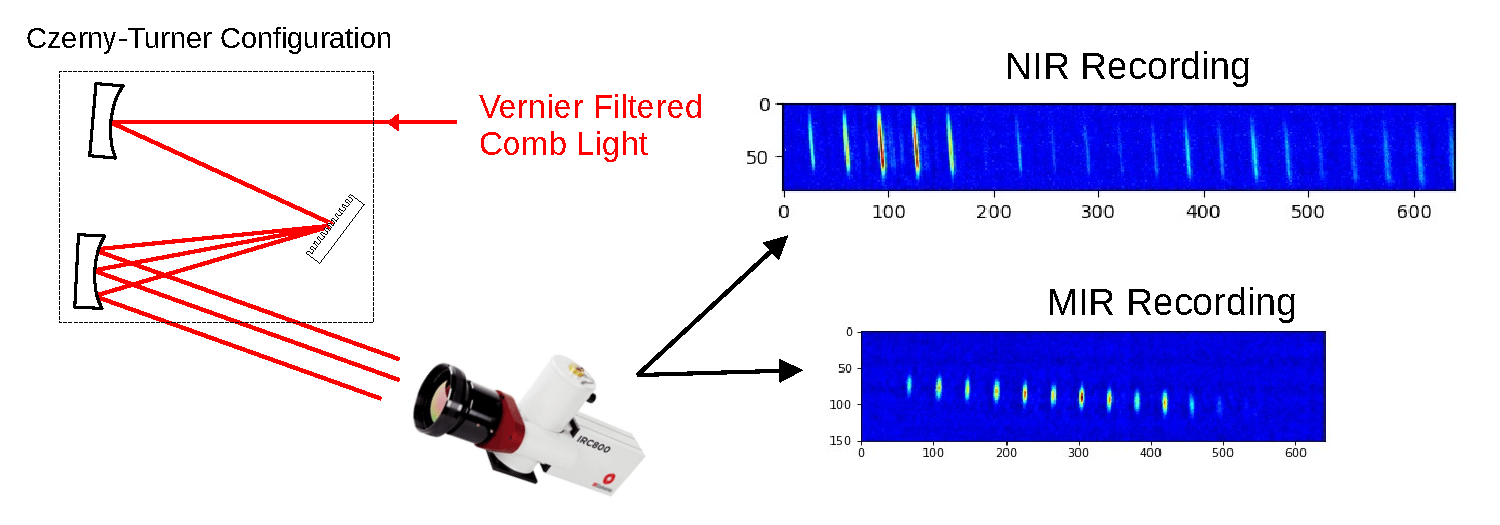
\includegraphics[width=0.85\linewidth]{diagrams/vernier_camera_detection}
		\caption{Detector used to spatially resolve the spectrally dispersed vernier orders. The same detector is shown used in the near-infrared (NIR) region from 1.5-1.7 {\textmu}m and the MIR region from 3.2-3.6{\textmu}m.}
		\label{fig:vernier_cameradetection}
	\end{figure}
	
	\subsection{Alternative Detection Schemes -- Replacing the Camera}
	In constructing the setup shown in Fig. \ref{fig:vernier_setup}, there are three main components which determine the main cost of building such a setup. These are the comb source, the cavity mirrors, and the detector. We do not count the grating or the spectrometer in this consideration, since the relaxed resolution requirements of the Vernier technique do not necessitate a premium quality spectrometer. In Ch. \ref{chap:mock}, we consider the use of a single photodiode as a position sensitive detector through the use of a newly proposed mechanical encoder.
	
	Such a scheme is can be directly applicable as a replacement detector for the expensive liquid-nitrogen cooled infrared camera shown in Figs. \ref{fig:vernier_setup} and \ref{fig:vernier_cameradetection}. An additional advantage to such a detector is that it can be operated at any wavelength where a sufficiently fast photodetector can be obtained, a benefit not shared by many spatially sensitive detectors.
	
	Vernier spectroscopy has already been performed using a single photodiode. One such scheme involve the scan of an aperture, such that only one Vernier order is observed at a time \cite{vernier_continuous_filtering}. This approach looses the multiplex advantage of Vernier spectroscopy \cite{ours_vernier, vernier_gohle}, and results in somewhat longer scan times. Another approach uses a Michelson interferometer to perform FTIR of the transmitted comb light near the exact matching condition \cite{vernier_MIR_fts}, and recently this technique was extended to yield broadband measurements of the cavity ringdown time \cite{modulated_ringdown_comb}, allowing for broadband and calibration-free measurements of intra-cavity absorption.
	
	We will briefly discuss how such techniques can be accomplished by locking the cavity-comb resonance. This allows us to introduce an operating regime which is highly compatible with the mechanical encoder proposed in Ch. \ref{chap:mock}.
	
	\section{Locked Cavity Detection}
	It was shown in Fig. \ref{fig:cavpdhlock} the tight locking of a CW laser to a cavity resonance using an electro-optic modulator. Similar techniques have been proposed for the locking of a comb-cavity resonance using a modulator \cite{book_yeCundifff_combs}, as well as swept-locking techniques which are well described in \cite{thorpe_dissertation}.
	
	Recently, the technique of modulated ringdown comb interferometry \cite{modulated_ringdown_comb} was demonstrated, showing that broadband and calibration-free measurements of intra-cavity absorption can be obtained using a Michelson interferometer as a detector. For this purpose, the processing of interferograms was modified from the traditional FTS. This is necessary because the technique uses sweep locking to hold resonance between the comb and cavity, and this type of locking generates a train of periodic pulses from the cavity with the same period as the cavity sweep. This modulated output causes difficulties with the traditional FTS interferogram processing.
	
	\begin{figure}[H]
		\centering
		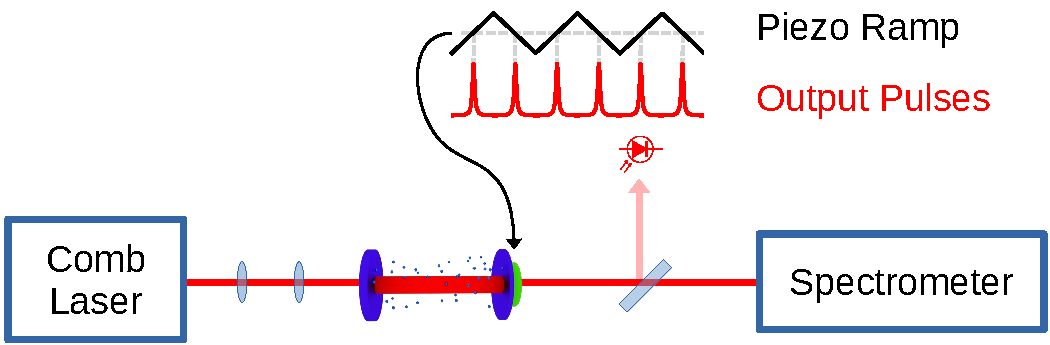
\includegraphics[width=0.85\linewidth]{diagrams/vernier_sweepLock}
		\caption{Simplified diagram of sweep locking. The cavity length is dithered slightly around the perfect matching length, where sharp pulses are observed in the cavity output. The output beam of the cavity is sampled by a photodetector, and locking electronics act to stabilize the offset of the cavity scan to generate a stable pulse train. The rigidity of the lock can be affected by altering the depth at which the sweep takes place. As the amplitude of the scan is decreased near the resonance length, more power is transmitted out of the cavity at the expense of lock stability.}
		\label{fig:verniersweeplock}
	\end{figure}
	
	
	
	\chapter{A POSITION SENSITIVE CHOPPER FOR BEAM PROFILING IN ONE DIMENSION} \label{chap:mock}
	We propose a mechanical device designed for one-dimensional imaging that functions similarly to a linear CMOS sensor but utilizes only a single photodiode. This is achieved through a specialized chopper disk, which encodes the position information of the beam into a time-varying intensity signal.
	
	\section{Mock Interferometer}
	The concept of this disk is similar to the device proposed by Mertz \cite{mock_Mertz_1960,mock_Mertz_1961} and theoretically investigated in \cite{mock_SELBY196621}. In the original design, the disk consists of a regular pattern of parallel slats. A light beam was passed through the disk and retro-reflected by a Littrow prism, which then passed through the disk a second time at an offset position. This process effectively imaged the disk onto itself at an offset position, creating an aperture that opens and closes at a frequency dependent on the beam's position. Consequently, the disk was intended to function as a position-to-frequency encoder.
	
	\begin{figure}[H]
		\centering
		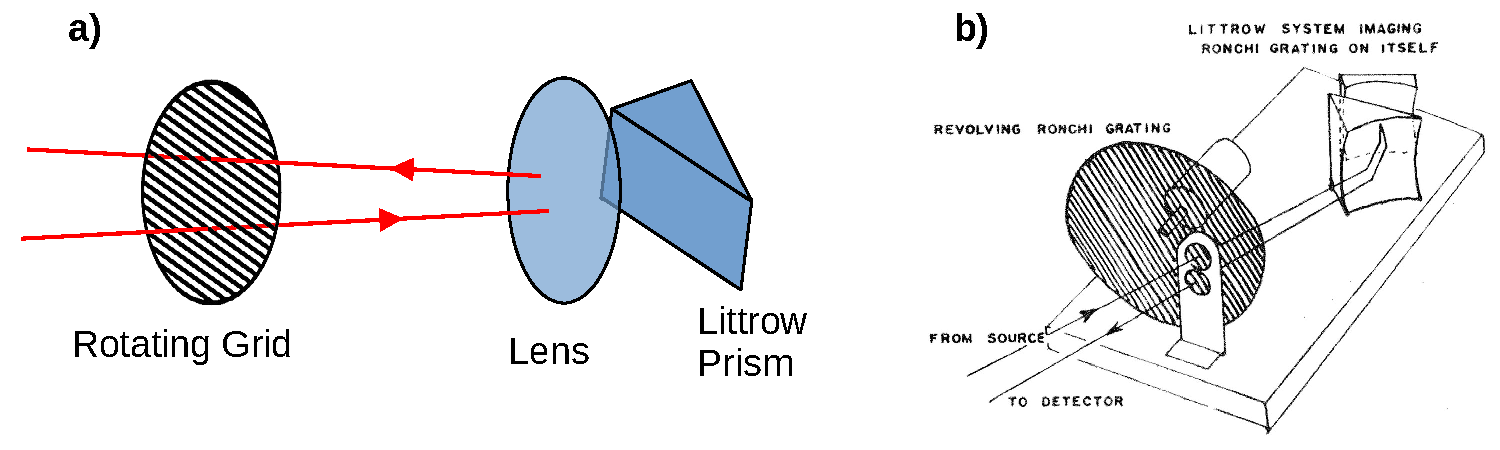
\includegraphics[width=1.0\linewidth]{diagrams/mock_OGdiagrams}
		\caption{Recreation of the diagram from \cite{mock_Mertz_1961}. A beam of light is first passed through the disk at a fixed position which is then retro-reflected and passed through the disk a second time at a position which depends on the wavelength. The position is imprinted on the photodetector signal.}
		\label{fig:mock_OGdiagram}
	\end{figure}
	
	\begin{figure}[H]
		\centering
		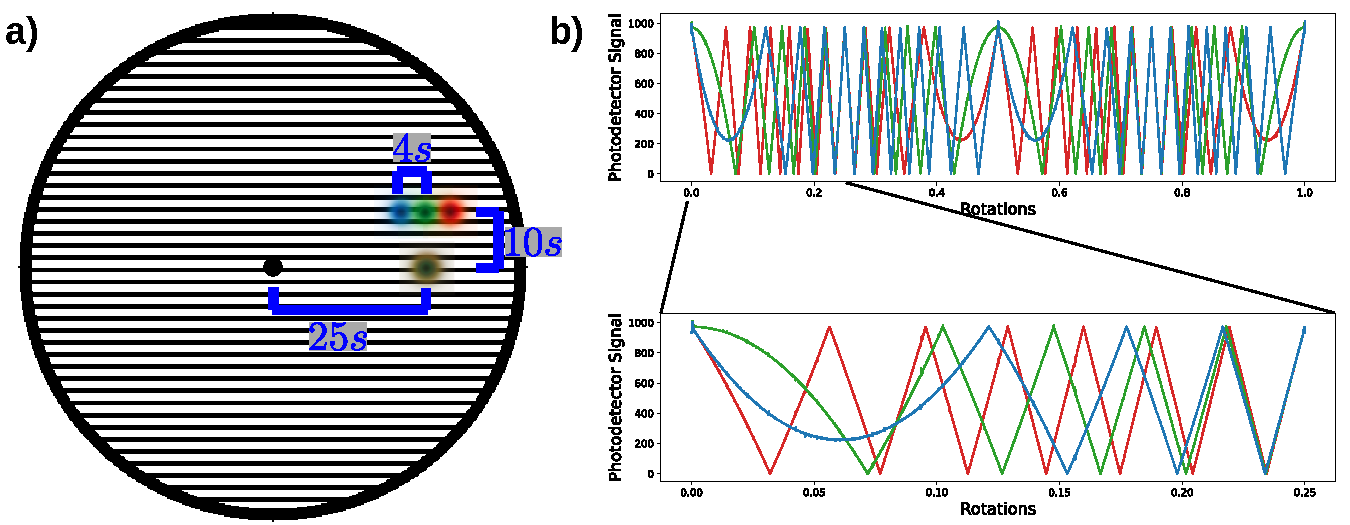
\includegraphics[width=1.0\linewidth]{diagrams/mock_originalSignal}
		\caption{Simulated signal of a large beam (encompassing several slats) making a double pass through the slatted encoder, similar to the original scheme proposed by \cite{mock_Mertz_1960,mock_Mertz_1961}. The beam makes an entrance at a distance of $25s$ away from the rotation center, where $s$ is the width of one of the slats. We suppose that the return beam carries information about some spectrally dispersive process. As such, we plot the variation of the signal with the spatial location of the return beam. The beams are modeled by a Gaussian profiles which are a distance $4s$ apart. It can be seen from the simulated photodetector signal in b) that there is indeed a strong variation of the signal structure with position, but it is not a pure sinusoidal encoding.}
		\label{fig:mock_OGsignal}
	\end{figure}
	
	\section{A Single Pass Multiplex Position Encoder}
	We propose an encoder similar to the mock interferometer, but utilizing only a single pass through the disk. Rather than using a beam that is large relative to the size of the apertures, we propose a configuration where the apertures are large relative to the size of the beam. We demonstrate that such an encoder disk is capable of recovering not only the absolute position of the beam, but also the amplitudes and positions of a superposition of multiple beams simultaneously.
	
	We make different assumptions regarding the light incident on the device. Since the original development of the mock interferometer, lasers have become established as essential tools for precision spectroscopy. Correspondingly, the use of large, collimated beams of incoherent light in spectroscopic applications has decreased in favor of laser-based techniques. A more advantageous beam geometry would be that of a small, focused Gaussian beam, or a superposition of such beams, as is found in the image plane of a Czerny-Turner monochromator.
	
	\begin{figure}[H]
		\centering
		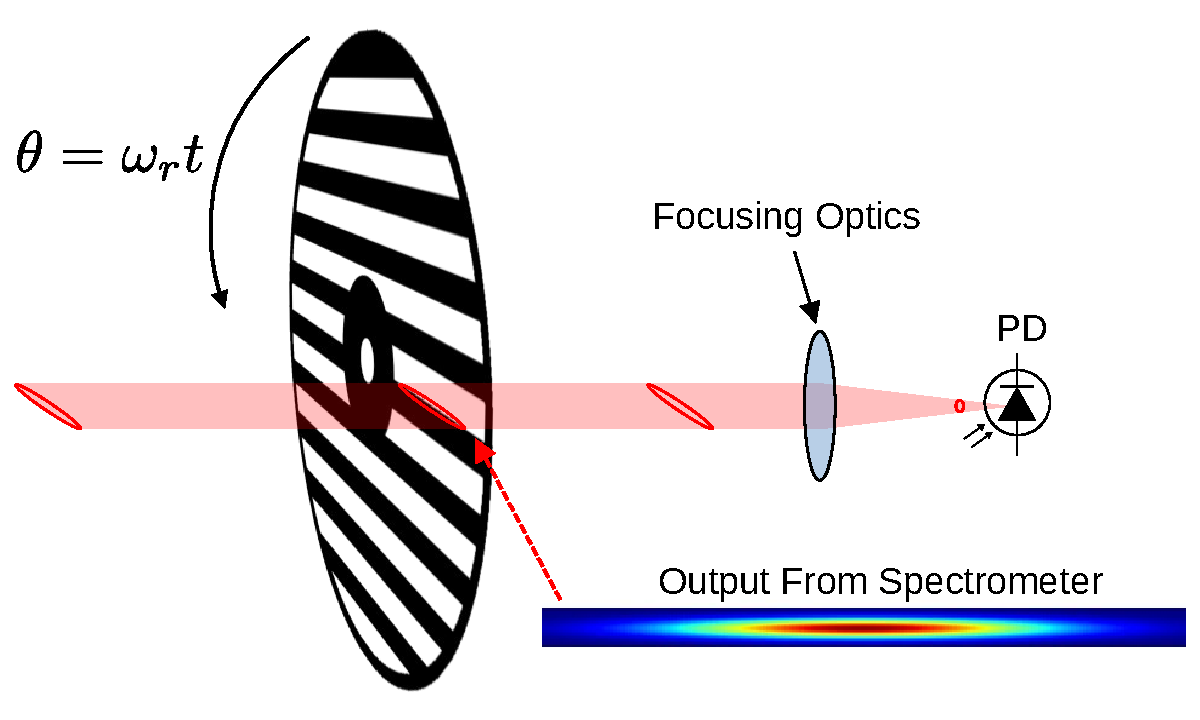
\includegraphics[width=0.5\linewidth]{diagrams/mock_config}
		\caption{Shown is a rotating mechanical encoder which transforms the spatial intensity information of the narrow line-like beam passing through it into time-varying fluctuations of the recorded photodetector signal. The focusing optics are arranged such that the intensity of the full beam is focused onto the small photodetector.}
		\label{fig:mocklongbeam}
	\end{figure}
	
	When the original scheme was proposed, the idea of recording the signal and performing advanced math operations on the analog waveform was considered in the form of hardware spectrum analyzers \cite{mock_Mertz_1961}. It was therefore desirable to have the signal resemble a sinusoid as close as possible so that the spectrum may be recovered using the Fourier transform. As evidenced by the simulated signal in \ref{fig:mock_OGsignal}, there is indeed some variation of the perceived signal frequency with beam position. The resolution with which separate frequency components can be resolved is limited due to the fact that that the long-term signal is actually only harmonics of the original disk rotation rate. In essence, trying to resolve the Fourier components too finely just results in the resolution of the disk rotation rate.
	
	Another issue with the original encoder scheme is that we require the input beam to be large enough to encompass several slats. This requirement automatically limits the resolution in many spectrometers, since the ideal location to measure the spectral information is at a sharp focus. A clean mapping of spectral information onto position information requires a sharp imaging of the angular dispersion onto a well-defined location, as in the Czery-Turner configuration.
	
	In the next section, we propose an encoder which is mechanically similar to the original Mock interferometer, but implemented with a single pass and a beam which is sharply focused in one dimension. Since the analysis of the photodetector signal does not need to be compatible with analog analyzer hardware, we use digital processing to recover the 1D spatial information of the beam passing through the encoder.
	
	\section{Theoretical Description of the Signal}
	In this section, we derive the equations used for the forward modeling of the photodetector signal by considering a theoretical transverse beam profile passing through the encoder. With an accurate forward model, it is possible in principle to reconstruct the beam profile from the photodetector signal.
	
	We do not focus on the absolute amplitude of the photodetector signals, as detectors typically report an uncalibrated voltage rather than the actual photonic intensity. Therefore, we include amplitude terms only when they are relevant to the relative contribution of different beams.
	
	We consider a system in which an infinitesimal beam passes through a rotating disk with parallel slats, and is subsequently focused onto a photodetector. An acquisition system records the resulting signal, ensuring that the light intensity is recorded proportionally over time.
	
	We define the periodic squarewave function $S(\xi)$ having the unitless argument $\xi$ and period of unity as
	\begin{equation}
		S(\xi) =
		\begin{cases}
			1 &\qquad \xi - \lfloor \xi \rfloor < 1/2 \\
			0 &\qquad \xi - \lfloor \xi \rfloor \ge 1/2 \\
		\end{cases}
	\end{equation}
	where $\lfloor \xi \rfloor$ denotes the floor function. We can describe the effect of the disk using a binary mask which yields an output of zero when a point $(x,y)$ is blocked by the disk and one when it is unblocked. At an angle of $\theta=0$, the mask is defined as:
	\begin{equation}
		M_{\theta=0}(x,y) = S\left(\frac{y}{2L}\right)
	\end{equation}
	
	In the following discussion, we model the photodetector signal as the scalar sum of the intensities of multiple static beamlets. By neglecting the disparate phases that would otherwise be summed within the Fresnel integral in Eq. (\ref{fresnel_integral}), we effectively remove diffraction and beating between adjacent spectral components. This simplification allows us to express the detector response, proportional to optical power, resulting from a finite-sized beam passing through the disk, as a sum of the intensities of many small beamlets not intercepted by the disk
	\begin{equation} \label{mock_integral_KE}
		P_\mathrm{det}(\theta) \,=\, \iint M_{\theta}(x,y)\, I_\mathrm{disk}(x',y') \; dx' dy'
	\end{equation}
	where $I_\mathrm{disk}(x, y)$ represents the intensity of a beamlet at position $(x,y)$ on the disk surface. This approximation is similarly common in knife-edge measurements \cite{book_gaussBeams_AtomsMolsOpticalPhys2} for forward modeling the photodetector signal, where a simple intensity mask is sufficient to characterize the beam to high precision \cite{beam_ISO_standard1, beam_ISO_standard2}.
	
	For a detector monitoring a beam passing through this encoder, we assume that the time dependence of the signal is due entirely to a constant rotation rate of the disk, $\theta(t) = -\omega t$. We consider a small beamlet centered at an arbitrary location on the disk, defined by polar coordinates $(R, \phi)$ relative to the rotation center. The angle $\phi$ is measured from the $0^\circ$ reference of the disk rotation, as indicated in red in Fig. \ref{fig:mockbeamlet}.
	
	\begin{figure}[t]
		\centering
		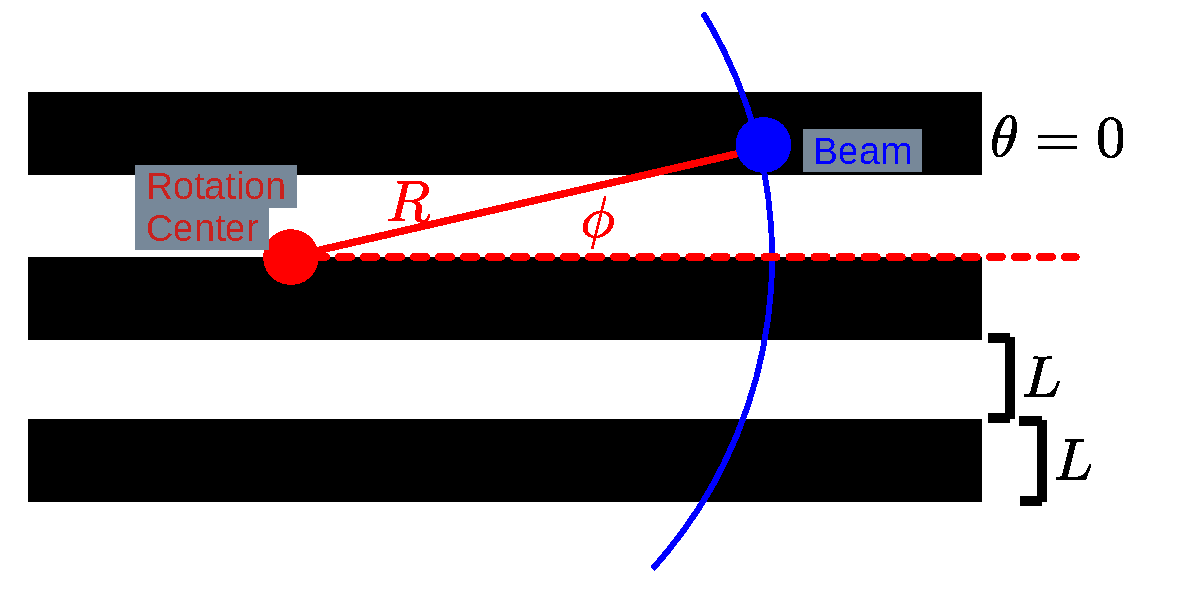
\includegraphics[width=0.5\linewidth]{diagrams/mock_beamlet}
		\caption{The signal of a point-like beam passing through the rotating encoder can be equivalently thought of as a point rotating around a stationary mask. If the slats are oriented along the x-axis, then the signal recorded by the photodetector is simply the stationary mask applied to the y-coordinate of this rotating point.}
		\label{fig:mockbeamlet}
	\end{figure}
	
	Rather than a rotating disk, it is perhaps easier to envision a point representing the beamlet location rotating around the origin, as depicted by the blue arc in Fig. \ref{fig:mockbeamlet}. The partial response of the photodetector due to this flickering beamlet is given by the square wave function of the $y$-coordinate of the beamlet position, which is rotated by an angle $\theta = \omega_\mathrm{r} t$. Here, $\omega_\mathrm{r}$ represents the angular frequency of the disk's rotation. For a beamlet located at $(x,y)$ with an area extent $dxdy$, this partial response is:
	\begin{equation} \label{mock_beamlet}
		dP_\mathrm{det}(t) = S\left(\frac{R}{2L}\sin\left(\omega_\mathrm{r} t + \phi\right)\right) I_\mathrm{disk}(x,y)\,dx dy
	\end{equation}
	The angular coordinate of the beamlet location, $\phi = \tan^{-1} (y/x)$, provides only a shift in the time axis of the photodetector signal, whereas the structure is entirely determined by the distance $R = \sqrt{x^2 + y^2}$ from the rotation center.
	
	This beamlet signal is clearly periodic with the disk rotation period $2\pi/\omega_r$, and it consists exclusively of the odd harmonics of this rotation frequency. While this may initially seem limiting, as Fourier analysis cannot directly resolve the separate contributions of several superimposed beamlet signals, a transformation of coordinates yields a signal that appears to have a continuously varying periodicity with the beamlet position.
	
	For a beamlet aligned along the axis $\phi=0$, the photodetector signal plotted against the sine of the rotation angle, $\sin\theta$, produces a square wave with a frequency that varies continuously with the distance from the rotation center, $R$. Although the disk consists of discrete spaces, the resulting signal structure varies continuously with the radial beamlet position.
	
	
	\subsection{Numerical Evaluation of the Signal}
	
	In our approximation, a finite-sized beam is represented by the sum of intensity contributions from many small beamlets, each characterized by an amplitude $A_i$. For such a beam, the detected light intensity at the photodetector, as a function of the disk angle $\theta$, can be expressed as
	\begin{equation} \label{mock_beamSum}
		P_\mathrm{det}(\theta) = \sum_i A_i S\left(\frac{R_i}{2L}\sin\left(\theta + \phi_i\right)\right)
	\end{equation}
	
	If the beam possesses an intensity profile $A(x,y)$ in Cartesian coordinates, the signal of a finite-sized beam can be simulated by dividing the two-dimensional plane containing the beam into a grid of points $\left(x_i, y_i\right)$. By summing the contributions from each grid point, we obtain increasingly accurate approximations of the signal as the grid size decreases.
	
	Starting from Eq. (\ref{mock_beamSum}), we perform a change of notation to dimensionless units, denoted by $x$ and $y$, which are related to the original coordinates $x'$ and $y'$ via the relations $x = \frac{x'}{2L}$ and $y = \frac{y'}{2L}$. In these dimensionless units, Eq. (\ref{mock_beamSum}) can be expressed as
	\begin{equation} \label{mock_beamGrid}
		P_\mathrm{det}(\theta) = \sum_i A(x_i, y_i) S\left[
		x_i\sin\theta + y_i\cos\theta
		\right]
	\end{equation}
	
	\subsubsection{Asymmetric Gaussian Beam}
	
	We consider the resulting time-dependent signal for an asymmetric Gaussian beam, where the transverse intensity profile at the intersection with the disk plane is described by
	\begin{equation} \label{mock_gaussProfile}
		A(x,y) = \exp\left[-\frac{\left(x-x_0\right)^2}{w_x^2} - \frac{\left(y-y_0\right)^2}{w_y^2}\right]
	\end{equation}
	In Fig. \ref{fig:mocksignalgauss}a, we plot the photodetector signal for a symmetric Gaussian beam at a fixed position of $x_0 = 3.1$, $y_0=0$ and varying widths. For an extremely small beam width, the result converges to Eq. (\ref{mock_beamlet}) for a single beamlet. As the width is increased, the binary pattern is smoothed while the overall structure remains intact. When the beam is translated along the radial direction of the disk, Fig. \ref{fig:mocksignalgauss}b demonstrates a sensitive dependence of the signal structure on the intersection location. Moreover, this dependence of the signal structure on the radial position is continuous, as illustrated by changing the beam position in increments smaller than the slat spacing $L$ in Fig. \ref{fig:mocksignalgauss}b.
	
	\begin{figure}[H]
		\centering
		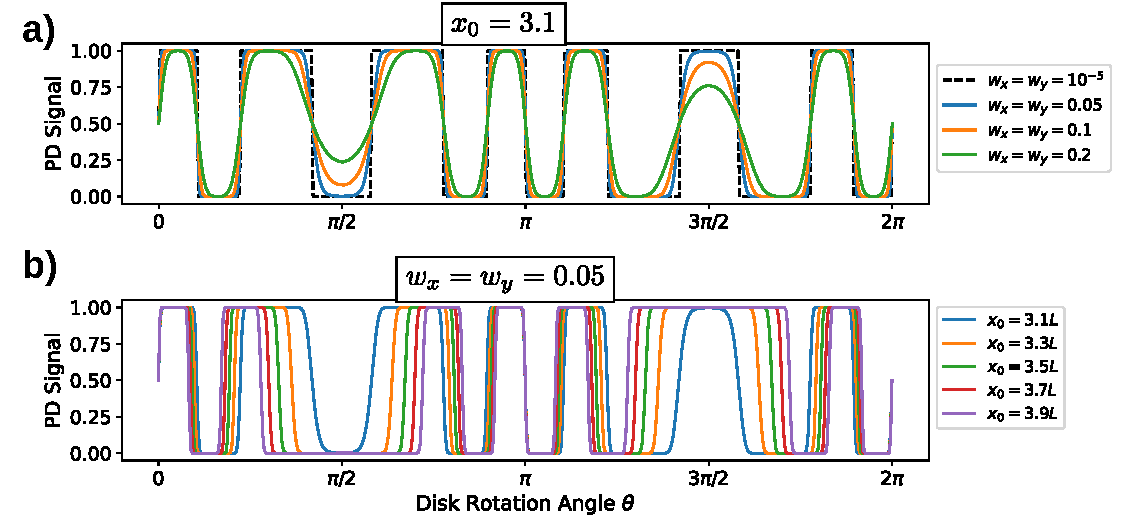
\includegraphics[width=0.75\linewidth]{diagrams/mock_signal_gauss}
		\caption{Shown is the intensity of a beam passing through the disk at different positions and sizes of the beam. In (a), the effect of changing the beam size is shown. It can be seen that the structure of the signal remains relatively similar, but with less clearly defined transitions as the beam becomes larger. In (b) it can be seen that the signal is very sensitive to the position of the beam. The curves shown represent the beam position changing over the distance $L$ corresponding to the slat size.}
		\label{fig:mocksignalgauss}
	\end{figure}
	
	
	\section{Position Spectrum}
	
	To evaluate the detector's utility for spectrometer applications, we consider a beam possessing a complex structure in one dimension while retaining a Gaussian profile in the other, which is characteristic of outputs from dispersion-based spectrometers. In a Czerny-Turner configuration, for instance, the wavelength-dependent angular dispersion of a diffraction grating is converted into position dispersion at a focal plane \cite{book_demtroder_2_experimental}, providing an ideal location for the encoder placement.
	
	For the remainder of this discussion, we assume that the beam possesses a complex profile along the $x$ direction. We suppose that the transverse profile can be decomposed into the product of two functions
	\begin{equation}
		A(x,y) = A_x(x) A_y(y)
	\end{equation}
	The function $A_x(x)$ is generally complex and may encode the position of an emission or absorption line from a spectrometer output, whereas the function $A_y(y)$ is typically a simple Gaussian resulting from the vertical focusing of the beam. In evaluating the sum in Eq. (\ref{mock_beamGrid}), it is necessary to ensure the grid is sufficiently fine to capture all essential features of $A_x(x)$.
	
	We evaluate the sum in Eq. (\ref{mock_beamGrid}) along the $x$, or $\phi=0$, axis, which yields:
	\begin{equation} \label{mock_posSpect}
		P_\mathrm{det}(\theta) = \sum_i A_x(x_i) \; S\Big[ x_i \sin\theta \Big] \exp\Big[-(y-y_i)^2 / w^2\Big]
	\end{equation}
	Although a closed-form solution for the infinitesimal photodetector signal contribution, $dP_\mathrm{det}(x_i, t)$, could in principle be derived for a given $x_i$ by integrating along $dy$, such an approach is not required. We note this to clarify that the beam profile in the $y$ direction is of secondary importance, as it primarily represents optical non-idealities such as spectrometer focusing. If the grid is sufficiently fine along the y-direction, then we expect that the above sum converges to such an expression.
	
	We define the quantity $\delta P_\mathrm{det}$ as the infinitesimal contribution to the photodetector signal resulting from performing the summation in Eq. (\ref{mock_posSpect}) along the $y$-direction for a fixed $x_i$ position, which allows us to express the total photodetector signal as:
	\begin{equation} \label{mock_x_beamlet}
		P_\mathrm{det}(t) = \sum_i a_i \; \delta P_\mathrm{det}(t, x_i)
	\end{equation}
	
	\begin{figure}[H]
		\centering
		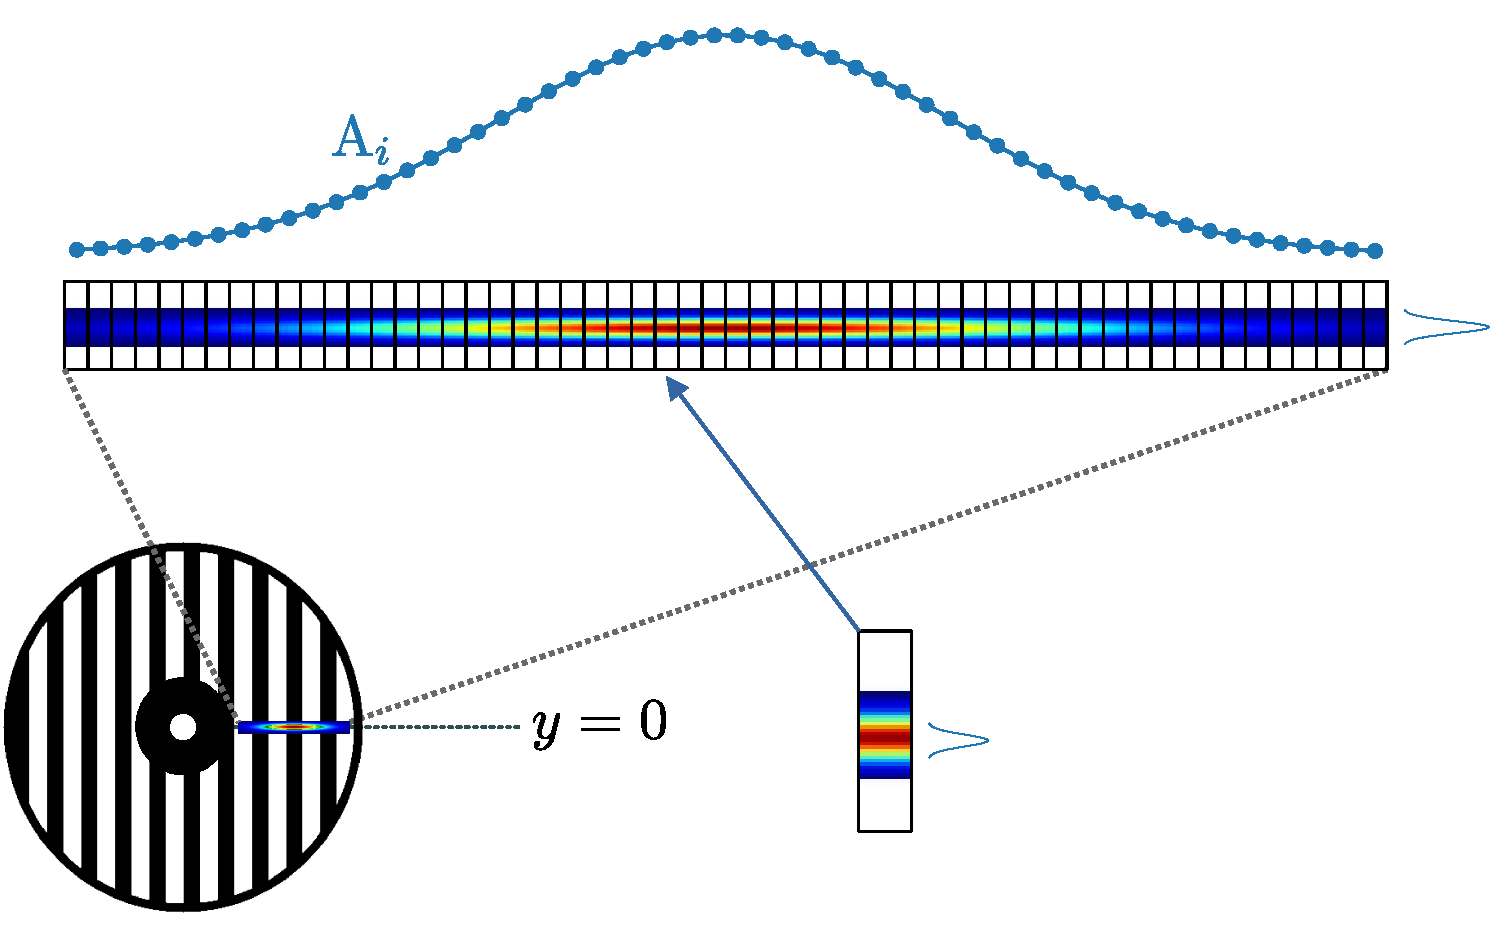
\includegraphics[width=0.65\linewidth]{diagrams/mock_positionSpectrum}
		\caption{Decomposition of the signal a sum of vertical slices, each having Gaussian shape along the $y$-direction and constant along the $x$-direction. The amplitudes of each of the vertical slices is represented in the upper graph by $a_i$, where the shape of an asymmetric Gaussian beam is shown.}
		\label{fig:mockpositionspectrum}
	\end{figure}
	
	\section{Decoding the Beam Profile}
	
	The challenge of decoding the beam profile lies in inverting the relationship expressed in Eq. (\ref{mock_x_beamlet}) to recover the spatial distribution $A_x(x)$ of a beam aligned along the $x$-axis. Because the detected signal is a linear superposition of contributions from discrete spatial elements, this reconstruction can be framed as a linear inverse problem.
	
	We begin by discretizing the potential spectrum into $M$ discrete spatial bins along the $x$-axis, where each bin $i$ is characterized by an unknown amplitude $a_i$ representing the integrated intensity of the beamlet at that position. To perform a reconstruction, we sample the photodetector signal at $N$ discrete time intervals $\{t_1, t_2, \ldots, t_N\}$ during a single rotation of the disk. By choosing the number of photodetector samples $N$ to be greater than the number of spatial bins $M$, we obtain an overdetermined system.
	
	To formalize this, we consider the response of the detector to an idealized "impulse" signal. Suppose the beam consists of a single, infinitely thin beamlet located at position $x_i$, which produces a photodetector signal defined as
	\begin{equation}
		%\delta P_\mathrm{det}(t, x_i) = \textbf{response at } t \textbf{ due to a delta-function input at } x_i
		\delta P_\mathrm{det}(t, x_i) = \text{the response at } t \text{ due to a delta-function input at } x_i
	\end{equation}
	
	In our discretized model, the $i^\mathrm{th}$ column of a disck design matrix $A$ represents the predicted temporal evolution of the signal if all light were concentrated at the $i^\mathrm{th}$ bin location. Thus, we define the elements of the matrix $A \in \mathbb{R}^{N \times M}$ as
	\begin{equation}
		A_{ji} = \delta P_\mathrm{det}(t_j, x_i)
	\end{equation}
	where $j$ indexes the time samples and $i$ indexes the spatial bins. Under this formulation, the vector of observed photodetode intensities $\vec{p} = [P_\mathrm{det}(t_1), P_\mathrm{det}(t_2), \ldots, P_\mathrm{det}(t_N)]^T$ is modeled as a linear combination of these basis responses,
	\begin{equation}
		\vec{p} = A\vec{a},
	\end{equation}
	where $\vec{a} = [a_1, a_2, \ldots, a_M]^T$ is the vector of unknown amplitudes to be recovered.
	
	Because we have intentionally set $N > M$, this system is overdetermined and may not have an exact solution in the presence of measurement noise or modeling errors. Following the derivation provided in the Appendix, we can resolve this by finding the least-squares solution (\ref{append_leastSquares}) that minimizes the residual error
	\begin{equation}
		\vec{a} = \underbrace{(A^T A)^{-1} A^T}_{\begin{matrix} \mathcal{R} \end{matrix}} \vec{p}
	\end{equation}
	%Shown in Fig. \ref{fig:mock_linear_decoding}, is the result of using this matrix to reconstruct a spectrum from a simulated noiseless photodetector signal.
	
	%\hl{\textit{DIAGRAM}}
	
	Above we have indicated the pseudoinverse matrix $\mathcal{R}$ which serves as a "reconstruction operator". While this analytic approach is mathematically elegant, its utility is limited by the extreme sensitivity of the $\mathcal{R}$ operator to any deviation from the ideal model. In a physical system, the reconstruction is subject to both additive measurement noise and multiplicative modeling errors. The latter are particularly insidious; they arise from fundamental mechanical and optical imperfections, such as imperfectly centered disk rotation, slat width non-uniformity, or beam axis misalignment.
	
	The severity of these errors is fundamentally tied to the condition number of the matrix $A^T A$. As the system resolution increases with a higher number of spatial bins $M$, the columns of $A$ represent increasingly overlapping temporal profiles. This increased correlation between adjacent basis functions drives the determinant of $A^T A$ toward zero, which renders the inversion operation increasingly ill-conditioned. In this asymptotic limit, the $\mathcal{R}$ operator acts as a high-gain amplifier for structural non-idealities, causing even infinitesimal errors in the assumed basis functions to produce catastrophic artifacts in the reconstructed spectrum.
	
	To overcome this, we must move beyond a static linear operator. By expanding the reconstruction mapping $\mathcal{R}$ into a nonlinear regime--specifically through the use of a learned, robust operator--we can develop a beam profile decoding protocol capable of compensating for these hardware-induced non-idealities and achieve stable reconstruction even at high spatial resolutions.
	
	\section{Nonlinear Reconstruction via Neural Networks}
	
	%In our implementation, we employ a multi-layer perceptron (MLP) architecture. A relatively shallow, fully connected MLP was found to be sufficiently capable of capturing the required nonlinearities without incurring prohibitive computational overhead. This architecture consists of an initial transformation layer that projects the high-dimensional time-series input into a latent feature space, followed by several intermediate layers that extract the complex correlations between temporal fluctuations and spatial intensities. The final layer then maps these learned features back into the $M$-dimensional space of the reconstructed beam profile.
	
	The transition from a linear operator $\mathcal{R}$ to a nonlinear reconstruction mapping represents a shift from analytic inversion to a statistical learning problem. While the pseudoinverse is constrained by the fixed, rigid structure of the matrix $A$, we propose an architecture that extends this concept through a series of interconnected layers. This model can be viewed as a generalized and highly flexible version of the linear operator, in which the weights of the network are not pre-calculated from a single matrix inversion, but are instead learned parameters optimized to map the input signal space to the desired output spectrum.
	
	The training process for this mapping is framed as a supervised learning task. We generate an expansive synthetic dataset by simulating the physics of the encoder disk across a wide range of operational parameters, which encompasses various beamlet positions, widths, and mechanical misalignments. Because these simulations are grounded in our established forward model, we possess access to "ground truth" labels: the exact spatial distribution $A_x(x)$ that produced each signal.
	
	To ensure that the resulting mapping is not merely an interpolator of specific datasets but remains a robust estimator capable of handling real-world uncertainty, we implement a stochastic training regime. During the optimization process, we introduce controlled perturbations to the input signals, such as additive Gaussian noise and random temporal jitter, to simulate the imperfect response of a real photodetector. This injection of noise during training acts as a form of regularization, preventing the model from over-fitting to the deterministic features of any single simulation and instead forcing it to learn the underlying invariant physics of the encoder.
	
	By leveraging modern hardware-accelerated computational frameworks, we can perform this optimization over millions of randomized signal instances. This allows us to sweep through a vast parameter space—effectively "training" the model on every conceivable operational deviation of the mechanical disk—which results in a reconstruction mapping that is both highly accurate and exceptionally resilient to the non-idealities of the physical apparatus.
	
	\section{Demonstration of Utility as a Position-Sensitive Detector}
	In this section, we demonstrate the effectiveness of the proposed encoder in place of a traditional position sensitive detector. We first make a comparison to another method which can characterize the 1D profile of a laser beam: the knife-edge method. We then demonstrate the proposed encoder as a spectrometer detector, and as a linear detector in applications of surface plasmon resonance (SPR).
	
	\subsection{Knife-Edge Comparison}
	
	As an initial test of the beam profiling ability of the encoder disk, we made a comparison to the standard knife edge method \cite{book_gaussBeams_AtomsMolsOpticalPhys2}. This was performed by translating a vertical knife edge, which is initially blocking a beam, at a known velocity out of the beam. The derivative of the photodetector signal (proportional to the total optical power received) with respect to the edge position gives the beam profile $I(x) \propto dP/dx = (dP/dt) / (dx/dt)$.
	
	In Fig. \ref{fig:mock_ke_comparison}, the configuration used to conduct the knife-edge measurements is shown, where it is placed as close as possible to the rotation plane of the disk. In this same figure, the resulting beam profiles compared to those obtained by the encoder are also shown.
	
	\begin{figure}[H]
		\centering
		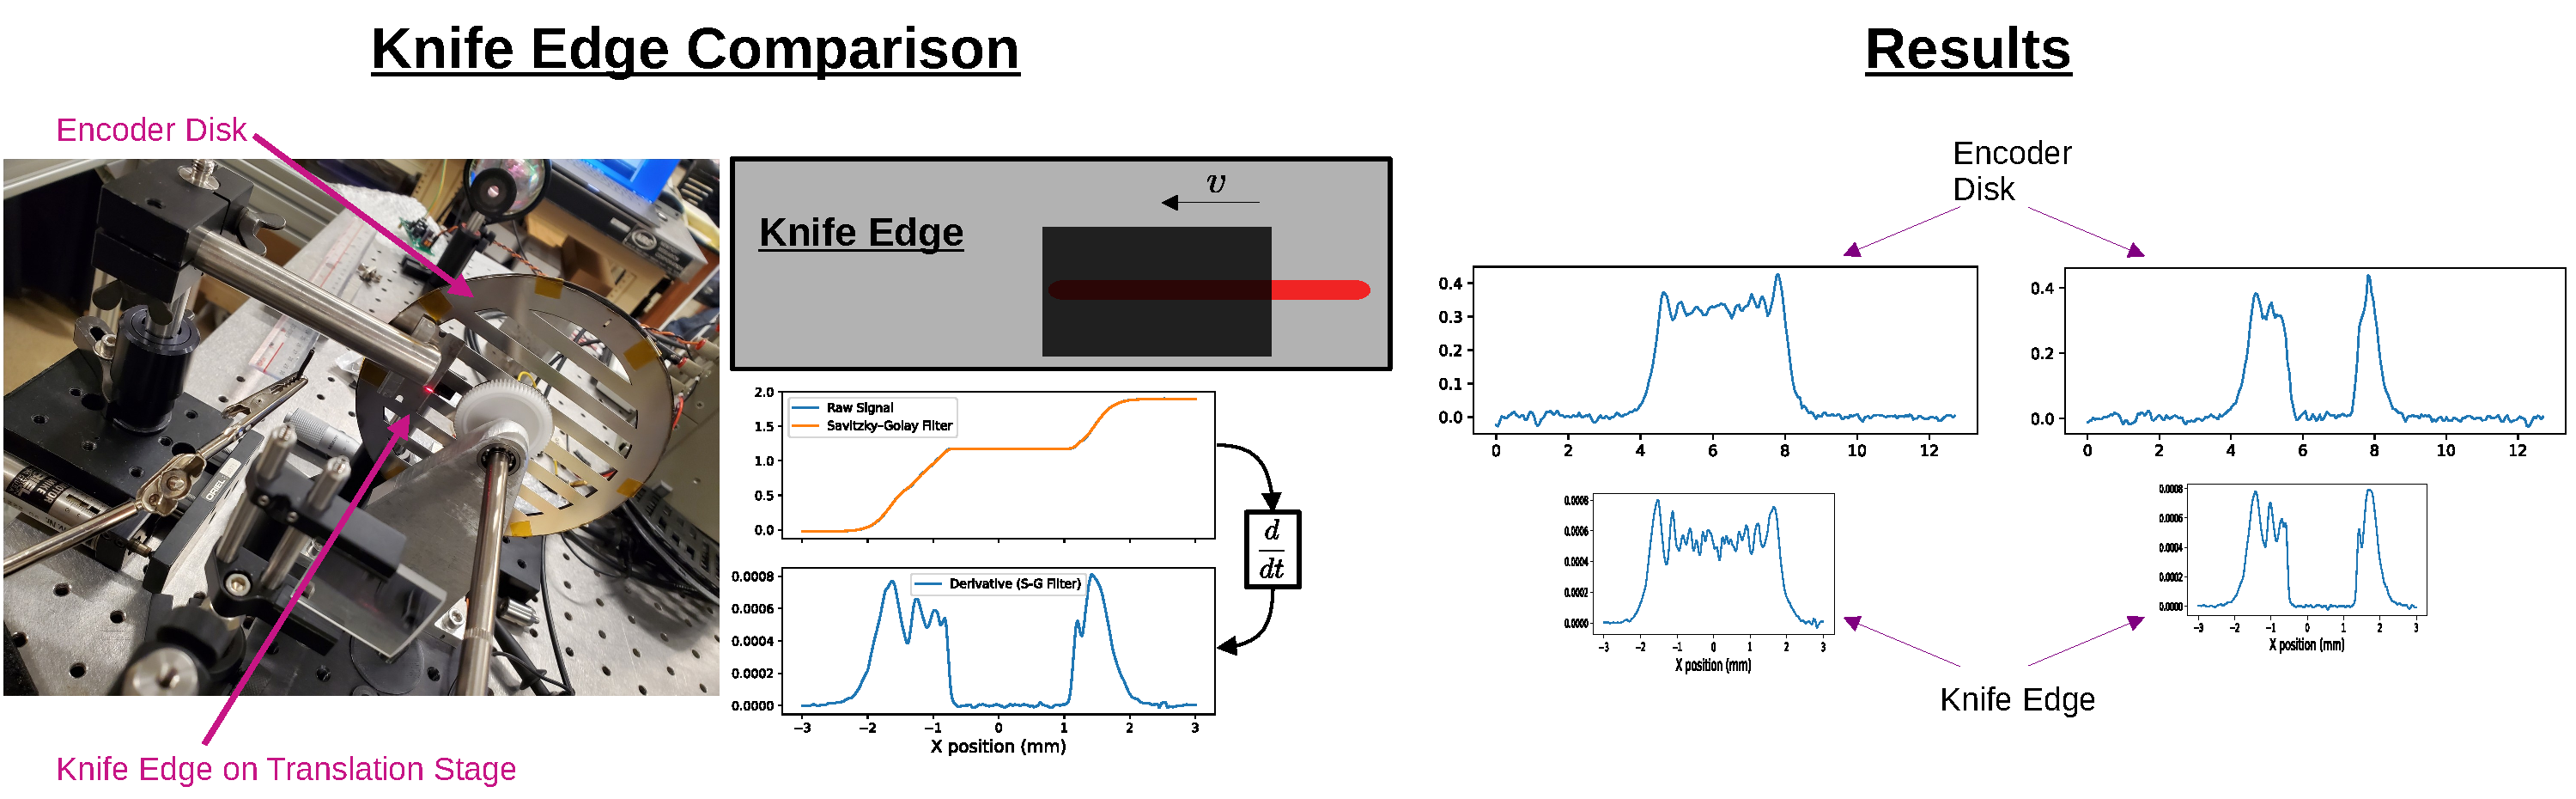
\includegraphics[width=1.0\linewidth]{diagrams/mock_KE_comparison}
		\caption{On the left image, the configuration used to conduct the knife edge comparison is shown. A razor blade is used as the edge and is mounted on a translation stage as close as possible to the disk's rotation plane. The beam profile is obtained by differentiating the resulting photodetector signal as the blade translates at a known velocity. On the right plots, the beam profiles obtained by the knife edge method and the encoder disk method are compared.}
		\label{fig:mock_ke_comparison}
	\end{figure}
	
	
	\subsection{Application to General Spectroscopy} \label{sec:mock_spectrometer_detector}
	
	In this section, we demonstrate the use of the proposed encoder as a general position-sensitive spectrometer detector. The demonstration of successful decoding in infrared spectrum regions is already a milestone, since high density linear sensor arrays are prohibitively expensive in this wavelength region. In the presented spectra, there are 1,024 points spread over an inch of sensing region, a figure competitive with commercial linear CMOS sensors. 
	
	\begin{figure}[H]
		\centering
		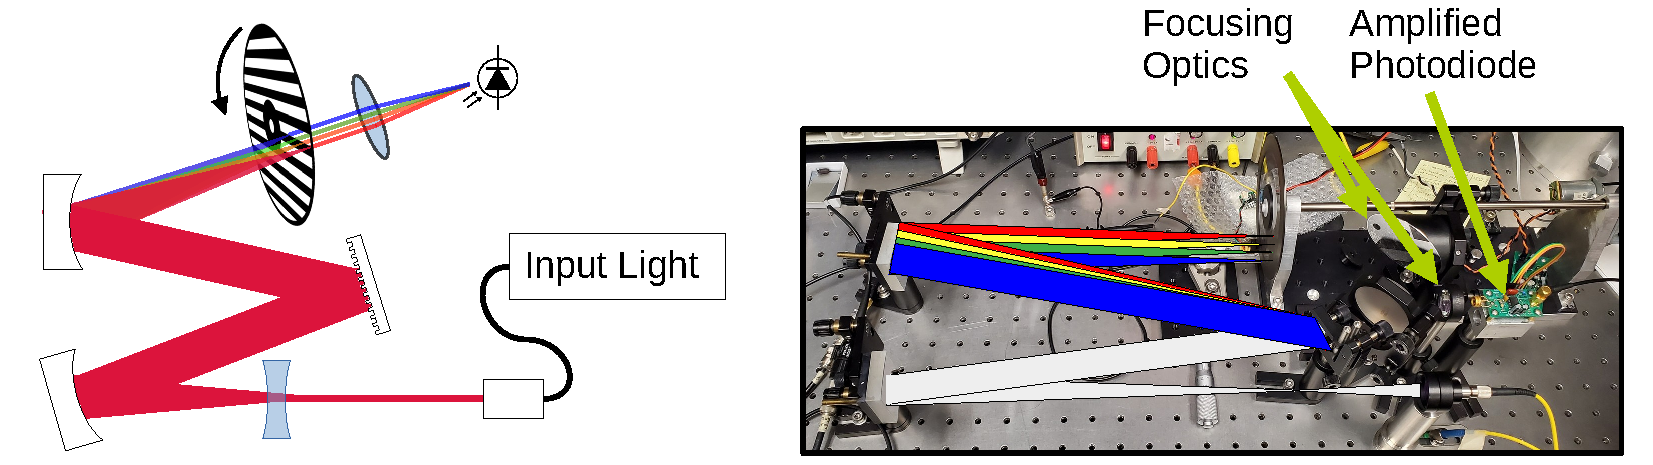
\includegraphics[width=1.0\linewidth]{diagrams/mock_spectrometerSchematic}
		\caption{Test platform for use of the encoder disk as a spectrometer detector. On the left, a Czerny-Turner spectrometer configuration is shown, where the encoder disk is placed in the focal plane of the spectrometer's output. The light passing through the rotating disk is detected by a single photodiode after being focused by two focusing elements (not shown), where the time-domain structure of the signal is used to decode the optical spectrum. On the right is a picture of the actual construction used to conduct the measurements.}
		\label{fig:mockspectrometerschematic}
	\end{figure}
	
	
	\begin{figure}[H]
		\centering
		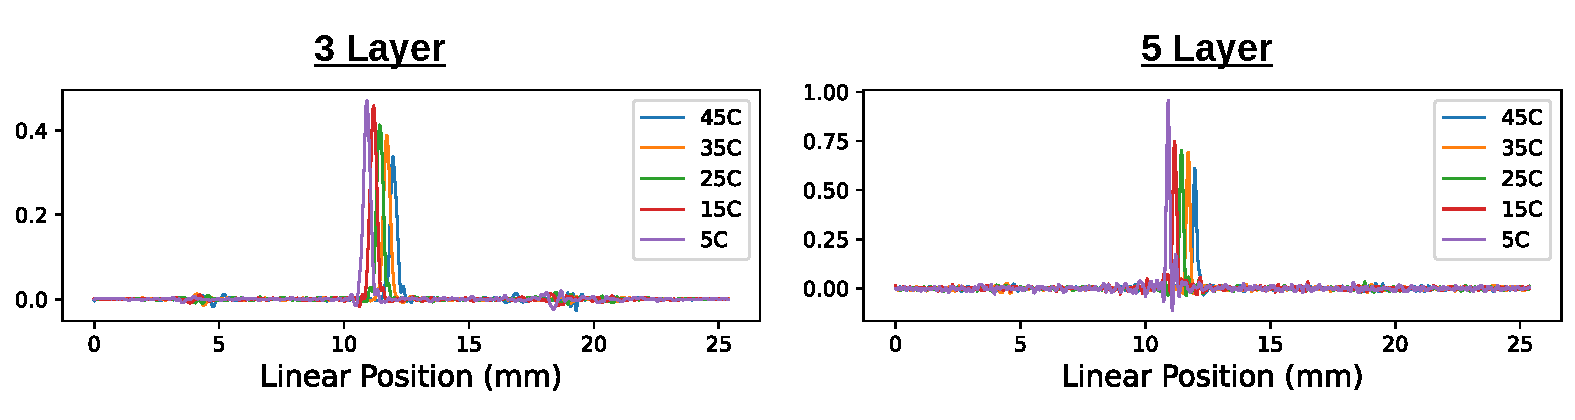
\includegraphics[width=1.0\linewidth]{diagrams/mock_result_CO2detuning}
		\caption{Spectrum of a DFB CW diode laser. The effect of tuning by changing the diode temperature is apparent in the decoded spectra. Here we compare a three layer and a five layer decoding network. It can be seen that the 3 Layer network seems to produce a higher signal to noise ratio with less artifacts, the 5 layer network seems to give an improved spectral resolution, as seen by the narrowing of the observed CW laser peaks.}
		\label{fig:mockresultco2detuning}
	\end{figure}
	
	\begin{figure}[H]
		\centering
		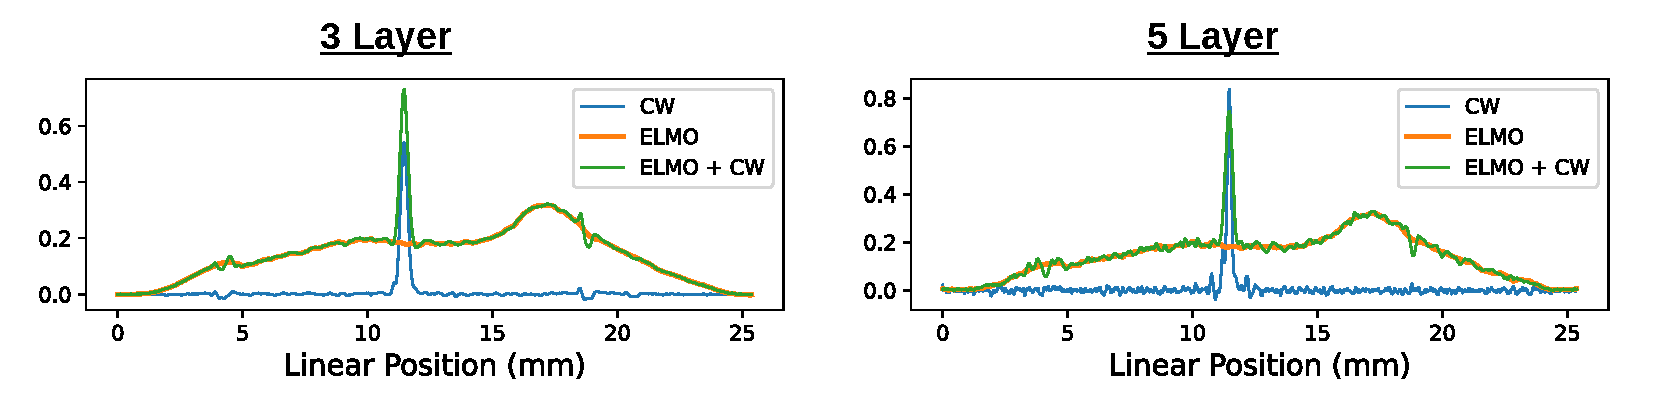
\includegraphics[width=1.0\linewidth]{diagrams/mock_result_elmoCWoverlap}
		\caption{Investigating the preservation of linearity in the decoded signal. Show three spectra: a narrowband CW laser, a broadband fs pulsed laser, and the two optical spectra superimposed. It can be seen from the decoded superimposed spectrum that linearity is not precisely preserved by the introduction of additional artifacts away from the CW peak. It is again seen that a higher number of layers gives increased resolution at the expense of increased artifact introduction.}
		\label{fig:mockresultelmocwoverlap}
	\end{figure}
	
	\begin{figure}[H]
		\centering
		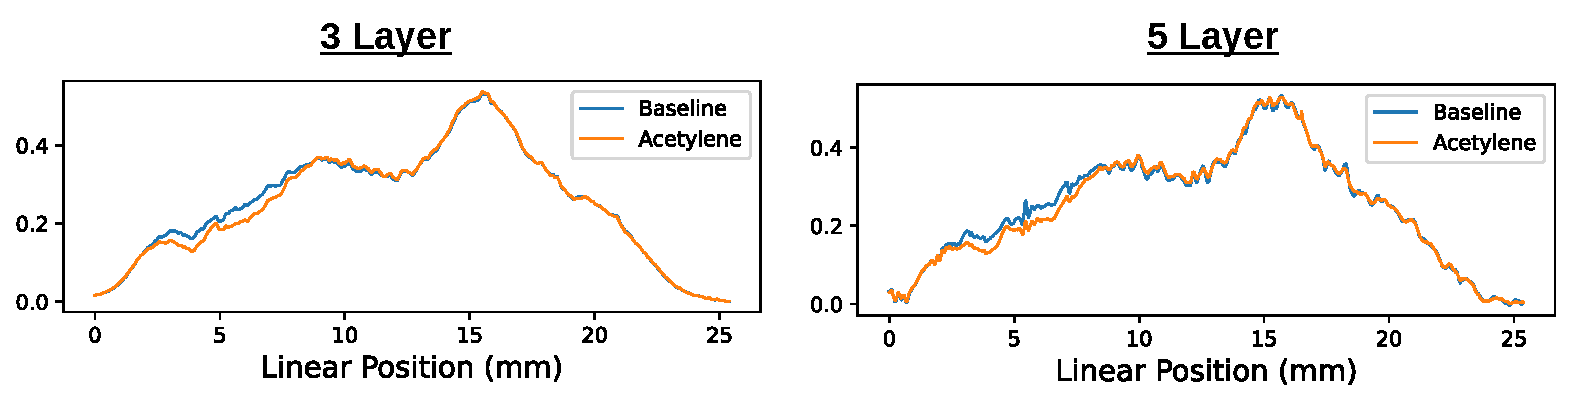
\includegraphics[width=1.0\linewidth]{diagrams/mock_result_acetylene}
		\caption{Measurement of an absorption spectrum. A broadband femtosecond laser spectrum is measured, allowed to pass through an acetylene absorption cell, and then measured again. The localized intensity dip due to acetylene absorptions can be seen.}
		\label{fig:mockresultacetylene}
	\end{figure}
	
	
	
	
	%\subsection{Suitability for Vernier Spectroscopy and Breath Analysis -- Replacing the expensive detector}
	\subsection{Application to Surface Plasmon Resonance}
	
	Another application of position sensitive detectors occurs in surface plasmon resonance (SPR) experiments \cite{spr_kolomenskii:97}. In such experiments, light is totally internally reflected from a glass interface which has deposited a thin layer of metal. This thin layer of metal causes results in a resonance condition where light at a particular angle suffers from attenuated total reflection (ATR). This ATR angle shows extreme sensitivity to the refractive index of the medium on the opposite side of the metallic film, enabling the construction of sensitive and specific sensors, some of which have been applied to breath analysis \cite{spr_breathAnal_review}.
	
	We demonstrate the applicability of our proposed encoder to the detection of the attenuated total reflection angle by constructing a typical SPR experiment and replacing the linear array sensor normally used for detection with a single photodiode and the encoder. Shown in Fig. \ref{fig:mocksprsetup} is a typical setup for such an experiment. A flat line beam is generated using a Powell lens, which is collimated along the expansion direction using a cylindrical lens. This laser line is focused onto a point of total internal reflection inside of a glass prism. This is done to sweep a range of angles encompassing the ATR angle. 
	
	This glass prism is placed against a commercial SPR sensor plate with index matching gel to act as the thin metal interface. On the back side of the sensor plate, a flow of water is obtained using an aquarium peristaltic pump. We attempt to detect the minute refractive index differences of the water by increasing the salt concentration. This is perceived as a shift of a minimum intensity dip caused by the attenuated total reflection. The amount of shift of this minimum can be used to determine the refractive index of the medium for sensing purposes.
	
	After the light passes through the prism it is recollimated using a cylindrical lens and then focused in the orthogonal direction by another cylindrical lens. This is done to get a tightly focused narrow line beam at the location of the disk plane. After passing through the disk, the light is focused onto the a large-area photodiode by a large plano-convex lens.
	
	Shown in Fig. \ref{fig:mockresultspr} is the result of decoding the photodetector signal with two different neural networks. In both cases, the shift of the minimum intensity can clearly be seen, indicating a successful detection of the refractive index shift of the salinated water.
	
	\begin{figure}[H]
		\centering
		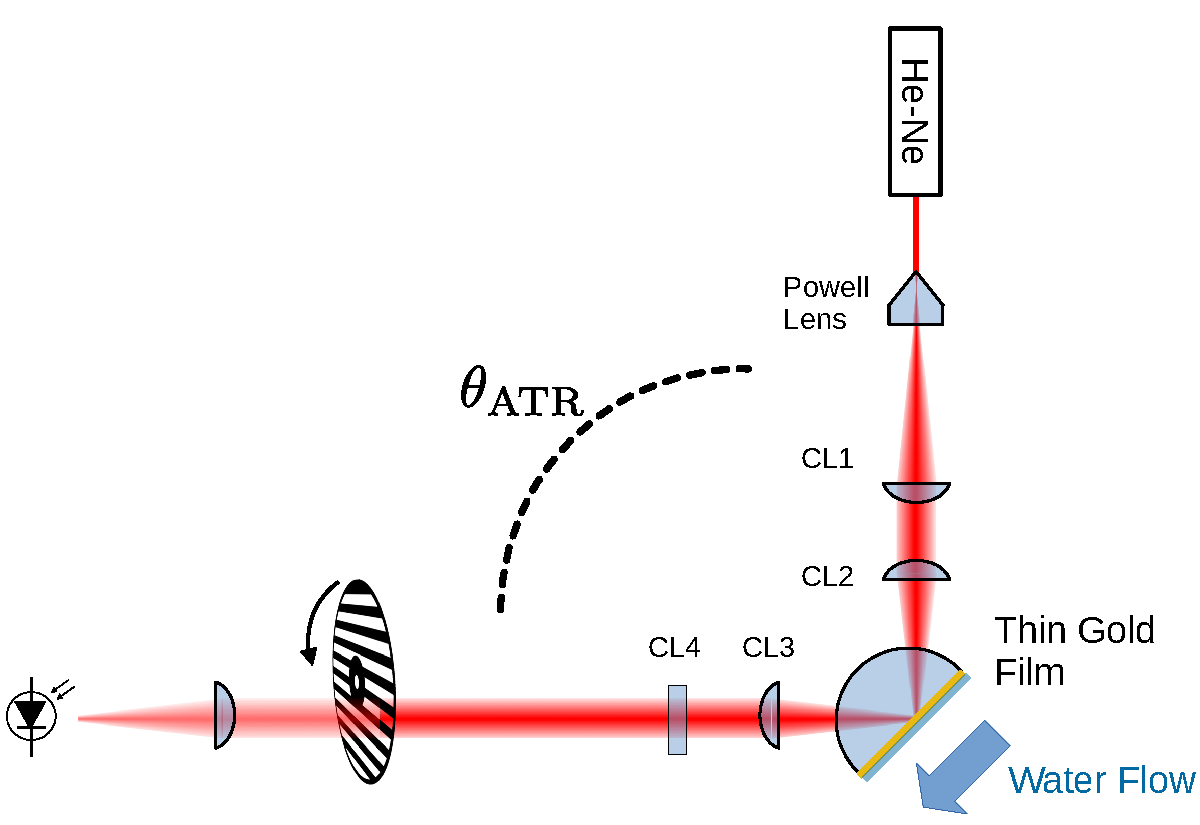
\includegraphics[width=0.9\linewidth]{diagrams/mock_SPR_setup}
		\caption{Use of the encoder disk in a surface plasmon resonance detection setup.}
		\label{fig:mocksprsetup}
	\end{figure}
	
	
	\begin{figure}[H]
		\centering
		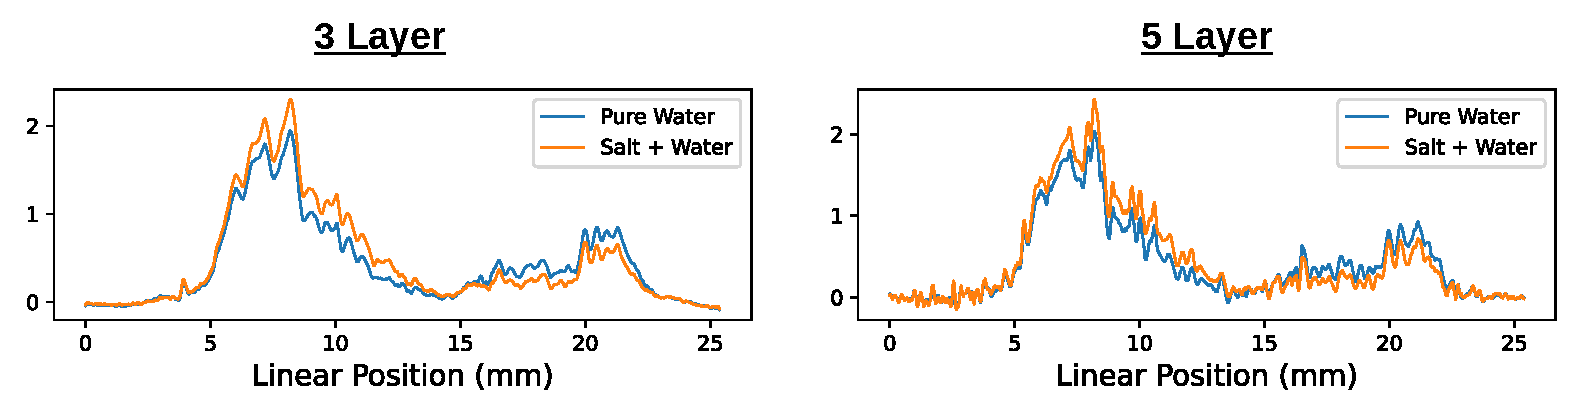
\includegraphics[width=1.0\linewidth]{diagrams/mock_result_SPR}
		\caption{The shift of the attenuated total reflectance (ATR) angle can be seen as the refractive index of the water is changed by increasing salt concentration.}
		\label{fig:mockresultspr}
	\end{figure}
	
	\chapter{SUMMARY OF WORK AND CONCLUSIONS}
	
	\section{Summary of Motivation}
	Optical breath diagnostics offer the potential for rapid, noninvasive assessment of human health. However, compact spectroscopic systems often suffer from challenges associated with wavelength calibration, instrument complexity, and quantitative concentration retrieval. The overarching goal of this dissertation was to investigate methods for calibration-free spectroscopic analysis and to develop techniques that support the realization of compact cavity-enhanced breath diagnostic platforms.
	
	
	
	\section{Summary of Major Results}
	The major results of this dissertation are given under the following four major headers
	
	\subsection{Improvement of NIR Spectroscopic References for Acetone}
	Using cavity ring-down spectroscopy, the absorption cross section for acetone near the peak absorption in the NIR was characterized with high precision in Sec. \ref{sec:acetone_peak}, both in wavelength and absorption scale. To improve the accessibility of this cross section information, we introduced an empirical model of the peak shape which characterizes the acetone absorption cross section in the region 1671.5-1675nm by five coefficients given in Table \ref{table:acetone_coeffs}. Additionally, we showed that the shape of this peak seems to be, to a large degree, unaffected by pressure broadening and collisional effects, indicating that the pressure independent cross-section model given by Eq. (\ref{acetone_model}) remains valid in a regime which is practical for breath analysis.
	
	We immediately improve on this proposed empirical model in Sec. \ref{sec:acetone_broadband} by conducting broadband measurements of the acetone cross section. The model of the narrowband NIR peak given in Sec. \ref{sec:acetone_peak} was used to calibrate the scale of the broadband cross section. Again, we give the results of these measurements as a set of empirically determined fit coefficients, some of which have been held fixed to enforce the high resolution wavelength information gained from the study of the narrowband peak in \ref{sec:acetone_peak}. To allow the cross section information to be modeled effectively in future studies, the coefficients of the broadband acetone absorption model, given in Table \ref{tbl:acetone_broadband_coeffs}, are also packaged as a Python function in \ref{sec:subsys_acetone_function}.
	
	\subsection{Advancements in On-line Wavelength Calibration}
	In Sec. \ref{sec:wl_tracking}, the dynamic wavelength reconstruction (DWR) method was introduced as a new way to process the fringes of a Michelson interferometer which is measuring a laser which is continuously scanning in wavelength, simultaneously with the interferometer scanning in delay. This method allows the continuously varying wavelength of the laser to be reconstructed from the fringes of the traveling interferometer. Such a method serves as a new method of processing interferogram fringes, distinct from the established methods of interferometric wavelength determination and Fourier transform spectroscopy (FTS), which is overviewed in Sec. \ref{sec:wl_FTIR}.
	
	In order to validate the DWR method, a simultaneous cross-validation was performed between the doppler-free hyperfine spectra of rubidium (Sec. \ref{sec:wl_results_HFS_DWRcomb}), and the beat-note with a repetition-rate stabilized frequency comb. To account for the free-running carrier envelope offset of the comb, an electronic ruler method was implemented in Sec. \ref{sec:wl_optical_detuning}, to measure the tuning of the probing laser's optical frequency in steps of one-half the comb repetition rate. This calibration was performed simultaneously with DWR measurements of the scanning laser, allowing a two-way calibration of the rubidium hyperfine structure scans. In this manner, the DWR method was shown to be competitive with both the frequency comb detuning method, and etalon-based tracking methods. The comb-based ruler method was itself independently validated and compared to etalon-based tracking methods in Sec. \ref{sec:wl_results_Xe}.
	
	Additionally, in \ref{sec:wl_wavelength}, a method is proposed for the efficient determination of wavelength ratios from standard wavelength measurements. This method, while not conceptually novel, is specifically optimized for digitally sampled interferograms and enables hardware-accelerated processing of the analog waveforms with minimal memory requirements. Wavelength determination is performed as soon as the analog waveform is collected, but yet with the virtual elimination of the counting error which plagues the simple formula zero-crossing formula (\ref{wl_wavelength_simple}).
	
	\subsection{Implementation of Inference-Based Wavelength Calibration Methods}
	Chapter \ref{chap:det} outlines a procedure for the calibration of laser wavelength scans directly from the measured absorption spectra, potentially eliminating the need for wavelength calibration altogether in compact cavity-enhanced absorption spectrometers. As presented, the method is applied to the specific case of cavity ring-down spectrometers (outlined in Ch. \ref{chap:CRDS}), and DFB diode laser sources.
	
	It was shown that when the method is used under appropriate measurement conditions, estimates of the laser detuning were found to be extremely accurate and competitive with high-precision wavelength measurement equipment. This wavelength accuracy translated into minimal loss of precision for the determined gas concentrations.
	
	In principle the procedure, (shown diagrammatically in Fig. \ref{fig:det_algorithmflowchart}), could be adapted to other laser sources with different wavelength control parameters. The method also does not rely on any specifics of the cavity ring-down technique and can, in principle, be applied to other instruments which measure absorption.
	
	\subsection{Analytic Spectrum Fitting Procedure}
	In Ch. \ref{chap:fitting_spectra}, we outline a procedure for the analytic determination of gas concentrations from the measurement of absorption spectra. This analytic determination relies on the use of the non-interacting gas approximation, outlined in Sec. \ref{sec:non_interacting_gas}. The advantage of this method is that the errors of the concentrations can be propagated directly from the spectral structure and measurement uncertainty. Examples of the mapping from spectral structure to concentration can be seen in the discussion surrounding Figs. \ref{fig:fit_overlap_twospec} and \ref{fig:fitoverlapacetonebaseline}. It is found that even in the case of highly overlapped spectra, precise concentrations of multi-species spectra can still be determined.
	
	A general weight function is proposed in Sec. \ref{sec:weighted_fit}, which allows the analytic fitting routine to be used to minimize error in a space which is nonlinearly transformed from absorption. The utility of this function is demonstrated for the case of cavity ring-down spectroscopy, where a transformation to logarithmic ring-down times is enacted by a special case of this weight function, appearing as Eq. (\ref{weight_function}). A reduction in bias of the fits which result from the use of this weight function is confirmed in Sec. \ref{sec:simulation}.
	
	\subsection{Demonstration of Novel Detection Schemes}
	In Chapter \ref{chap:mock}, we propose a novel type of encoder disk which allows one dimensional imaging of a beam with a resolution comparable to commercial linear CMOS sensors. The geometry of the disk is based on a concept of the mock interferometer, but the geometry of the beam and its interception with the disk are modified to greatly increase the convenience of the device as a linear sensor.
	
	It is demonstrated in Sec. \ref{sec:mock_spectrometer_detector} that the proposed encoder disk is capable of serving as a practical spectrometer detector, achieving a pixel density of 1024 px/inch. We additionally show that the encoder disk can serve as a replacement detector for surface plasmon resonance-based sensors and as a potential detector for use in Vernier spectroscopy. These demonstrations show that the proposed encoder disk has potential applications in the context of building inexpensive spectrometers for breath diagnostics.
	
	A powerful feature of this detection scheme is that it enables position-sensitive beam measurements in wavelength regions where no such detectors exist. Since all that is required is a single optical power sensor, a much larger range of devices is enabled to be used in these regions.
	
	\section{Scientific Conclusions}
	From the preceding major results, the following conclusions are made
	\begin{itemize}
		\item Quantitative near-infrared acetone spectroscopy was found to be practical across the approximate broadband wavelength region from 1650 to 1800 nm, with optimal sensitivity and concentration retrieval performance occurring within the narrower region from 1671.5 to 1675nm.
		
		\item A scanning Michelson interferometer, typically employed for fixed-wavelength measurements, can be adapted to enable continuous tracking of time-dependent laser wavelength during spectroscopic scans.
		
		\item The impact of spectral overlap on concentration retrieval precision is fundamentally determined by the structure of the overlapping spectral features and can be quantitatively predicted prior to measurement.
		
		\item Laser wavelength calibration can be inferred directly from measured absorption spectra with sufficient accuracy to support quantitative concentration retrieval in cavity-enhanced spectroscopy sourced by DFB diode lasers, with performance comparable to high-precision external wavelength metrology.
	\end{itemize}
	
	\section{Limitations}
	The limitations of the methods developed in this dissertation are presented in the context of the individual investigations in which they were introduced. Accordingly, the following sections discuss the primary constraints and assumptions associated with each major component of the work.
	
	\subsection{Acetone Cross Section Investigation}
	It was found that during this investigation, there was significant interaction of acetone vapor with the aluminum walls of the measurement chamber. This was further investigated in Sections \ref{sec:acetone_drift} and \ref{sec:acetone_broadband_drift}. This contamination was observed during the measurements of the acetone cross section magnitude and forms one of the biggest confounding factors in its determination. Care was taken to minimize the effect, but it was not eliminated. Any error in the initial cross-section magnitude determined in Sec. \ref{sec:acetone_peak} propagate into the broadband model, since the same calibration is shared.
	
	The broadband measurement of the acetone cross section did not provide an independent measurement of the cross-section magnitude, preventing cross-validation of the two measurements. Instead this was performed by comparison of the spectral shape alone. Additionally, these measurements were conducted near the edge of the optical bandwidth of the broadband laser. This prevented us from measuring the full extent of the broadband absorption feature. To ensure that our reported empirical model captures the line wings all the way down to near zero absorption, we stitched our measured data with that appearing in the PNNL database.
	
	\subsection{Dynamic Wavelength Recovery (DWR)}
	While we proposed an outlined method for performing the dynamic wavelength calibration from the fringes of a scanning Michelson interferometer, we did not explicitly compare optimal methods for evaluating the phase derivatives which appear in the wavelength tracking equation (\ref{wl_tracking_equation}). Additionally, we did not give an optimal recipe for discretizing the wavelength tracking equation in terms of the analog waveform samples.
	
	Difficulty was encountered when using this method in conjunction with DFB diode lasers when tuning over an extended range. Although the working principle was demonstrated by tuning the laser diode temperature, a combination of hysteresis and time-lag mean that the laser diode temperature is a less versatile tuning parameter than the laser diode current. Performing DWR measurements of a laser having its wavelength tuned by continuous adjustment of current was prevented by the lack of a laser diode controller which simultaneously gives this continuous tuning ability and the required current stability.
	
	\subsection{Wavelength Inference Method}
	In discussing the method of wavelength calibration inference presented in Ch. \ref{chap:det}, no attempt was made to connect the model of diode laser detuning to the underlying physics of the device. As such, it was not determined if the model functions used for the diode laser detuning are of the optimal form.
	
	\subsection{Beam Profile Encoder}
	While we provided an initial demonstration of the practical utility of the encoder disk proposed in Ch. \ref{chap:mock}, we did not give a rigorous comparison of different network architectures. 
	
	\section{Future Work}
	Throughout the investigations in this work, many avenues of investigation were left unexplored.
	
	A follow-up investigation should focus on the interaction of acetone vapor in different storage conditions, with a particular emphasis on surface interactions with the storage container. Whether the transient effects of the NIR acetone absorption can give systematic effects to the characterization of breath samples is still a question that is not completely answered by this work. Additionally, it is unclear whether the presence of other species, especially water vapor, have an effect on the broadband shape of the NIR acetone absorption, or the transient behavior of this absorption.
	
	Further work on development of the dynamic wavelength reconstruction (DWR) method should be performed to find a procedure to optimally discretize the wavelength tracking equation and its integration. This investigation should be coupled with the finding the best method to evaluate the phase derivative terms in the wavelength tracking equation. Additional demonstrations of this technique with diode lasers and cavity ring-down spectroscopy would be easily achieved with a laser diode controller which enables low-noise continuous sweeps of the laser diode current.
	
	The wavelength inference method could greatly benefit from an in-depth investigation into the physical mechanisms of the laser diode wavelength tuning behavior. A physically motivated tuning model would be superior to the ad hoc functions used to describe the tuning behavior. This could allow more efficient use of the number of coefficients used to describe the tuning behavior.
	
	An investigation into the optimal decoding network architecture for the proposed beam profile encoder disk would greatly assist future devices constructed using this sensor concept. This investigation should take into account mechanical imperfections of the disk and the laser alignment. Additionally, the pattern of slats for encoding of the position information onto the time-domain photodetector signal is most likely not completely optimal for one-dimensional imaging. 
	
	\cleardoublepage
	\phantomsection
	\addcontentsline{toc}{chapter}{REFERENCES}	

	%\bibliographystyle{natbib}
	\bibliographystyle{unsrt}
	%\bibliographystyle{srtnat}
	
	\renewcommand{\bibname}{REFERENCES}
	\bibliography{diss, acetone}
	
	\phantomsection

\chapter{SUBSYSTEMS AND SUBROUTINES}
In this chapter, we describe several subsystems and mathematical procedures which were used throughout this work.

\section{A Fringe Counting Method for the Determination of Wavelength Ratios} \label{sec:wl_ratios}
When a laser of known wavelength is used in addition to the laser being measured, the motion of the stage can be tracked and accounted for by extracting the interferogram phase. We consider a function of the form
\begin{equation}
	f(t) = A \cos(\phi(t)) + B
\end{equation}
which resembles the functional form of the interferogram in equation (\ref{wl_sig_monochromatic}). Here the phase function $\phi(t)$ is in general non-linear, and represents the case where the moving arm of the interferometer does not proceed at a constant velocity. An estimate for $\phi(t)$ can be obtained by counting the number of oscillations in the signal. A simple way to do this is to high-pass filter the signal, which effectively removes the offset $B$, and then counting the zero crossings. Every time the high-passed signal crosses zero, the phase is known to have incremented by $\pi$. In this manner, we can build up a sampled version of the $\phi(t)$ phase function.

The interferogram of a monochromatic source given in (\ref{wl_sig_monochromatic}) has the phase function for the reference laser
\begin{equation}
	\phi_\mathrm{ref}(t) = \frac{2\pi}{\lambda_\mathrm{ref}}\delta(t) + \phi_0
\end{equation}
Similarly, the test laser gives an interferogram with the phase function
\begin{equation}
	\phi(t) = \frac{2\pi}{\lambda}\delta(t) + \phi_1
\end{equation}
Using the reference phase to eliminate the optical phase delay $\delta(t)$, the phase function of the test laser interferogram is
\begin{equation} \label{wl_phase_slope}
	\phi(t) = \underbrace{\frac{\lambda_\mathrm{ref}}{\lambda}}_{\mathclap{\text{Slope}}}\phi_\mathrm{ref}(t) - \underbrace{\frac{\lambda_\mathrm{ref}}{\lambda}\phi_0 + \phi_1}_{\mathclap{\text{Offset}}}
\end{equation}
When the phase of the test laser interferogram is written in terms of the refeference laser interferogram phase, the slope of the resulting straight line is the ratio of wavelengths. It is this observation that motivates the following procedure.

We describe a procedure for estimation of the ratio of two wavelengths for two digitally sampled interferograms. The procedure is roughly broken down into four steps
\begin{itemize}
	\item Input Filtering
	\item Zero crossing detection
	\item Interpolation
	\item Slope determination
\end{itemize}

The interferogram recordings themselves are considered to be a series of digital samples of the analog waveforms, both sampled at the same interval $t_s$. If the test laser interferogram is $I(t)$ and the reference laser interferogram is $I_\mathrm{ref}(t)$, then the respective digital samples, $y_m$ and $r_m$, should ideally be given by samples of the analog waveforms at regular intervals
\begin{eqnarray}
	y_m = G I(m t_s) && r_m = G I_\mathrm{ref}(m t_s)
\end{eqnarray}
The value of the gain $G$ is of no importance in what follows, and in fact may be different for the two signals.

\subsection{Input Filtering}
The interferogram signal, given by equation (\ref{wl_sig_monochromatic}), is recorded as the intensity of light emerging from a Michelson interferometer as the delay arm is scanned, and naturally has a DC offset which must be removed in order for the zero-crossing method to be used for tracking the phase. This can be done by the analog electronics which precede the digital acquisition device, but often times a small residual offset can still remain. For this reason, it is necessary to digitally filter the signal to remove any remaining offset.

For reasonably well behaved signals, this offset removal can be as simple as subtracting out the mean of the signal values. However, it may be necessary to apply a proper high-pass filter to remove offending artifacts.

\subsection{Zero Crossing Detection}
The phase of the interferograms are built using the fact that every time a zero crossing of the oscillatory function crosses zero, the phase is incremented by a value of $\pi$. Given the sampled interferogram signal $y_m$, the times $\tau_n$ where the zero crossings occur give samples of the phase function
\begin{equation}
	\phi(\tau_n) = n\pi + \phi_0
\end{equation}

It is then desirable to obtain from a digitally sampled signal $y_m$ approximations of the zero crossing times. In general the zero crossings do not occur exactly at the sample times, but between two samples. The two samples before and after the zero crossing are opposite in sign, and this can easily be detected with the condition that $y_m y_{m+1} < 0$. When the sample number $m$ is found, where the zero crossing lies between the time $t_m = mt_s$ and $t_{m+1} = (m+1)t_s$, the zero crossing time can be found by assuming a simple linear interpolation of the signal. This gives
\begin{equation}
	\tau_n = mt_s + t_s \frac{y_m}{y_m - y_{m+1}} 
\end{equation}
Here the number $n$ increments by one each time a zero crossing is encountered. The process of zero crossing determination is summarized in Fig. \ref{fig:wlzerocross}. We perform this process also on the reference interferogram to obtain its zero crossings as
\begin{equation}
	\tau^{\mathrm{ref}}_n = mt_s + t_s \frac{r_m}{r_m - r_{m+1}} 
\end{equation}

\begin{figure}[H]
	\centering
	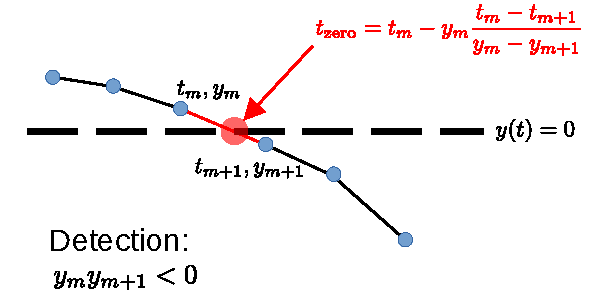
\includegraphics[width=0.65\linewidth]{diagrams/wl_zeroCross}
	\caption{Zero crossing detection in a digitally sampled interferogram, where linear interpolation of the signal is used to improve the timing of zero-crossing detection. The timing of these zero crossings entirely determines the information extracted from the interferograms in our implementation of the proposed procedure.}
	\label{fig:wlzerocross}
\end{figure}

\subsection{Interpolation}
Motivated by equation (\ref{wl_phase_slope}), we seek the phase of the test laser interferogram in terms of the reference laser interferogram phase. This can be done by interpolating the reference laser interferogram phase at the times of the test laser interferogram zero crossings. The procedure is outlined in Fig. \ref{fig:wlphaseinterpolation}.

\begin{figure}[H]
	\centering
	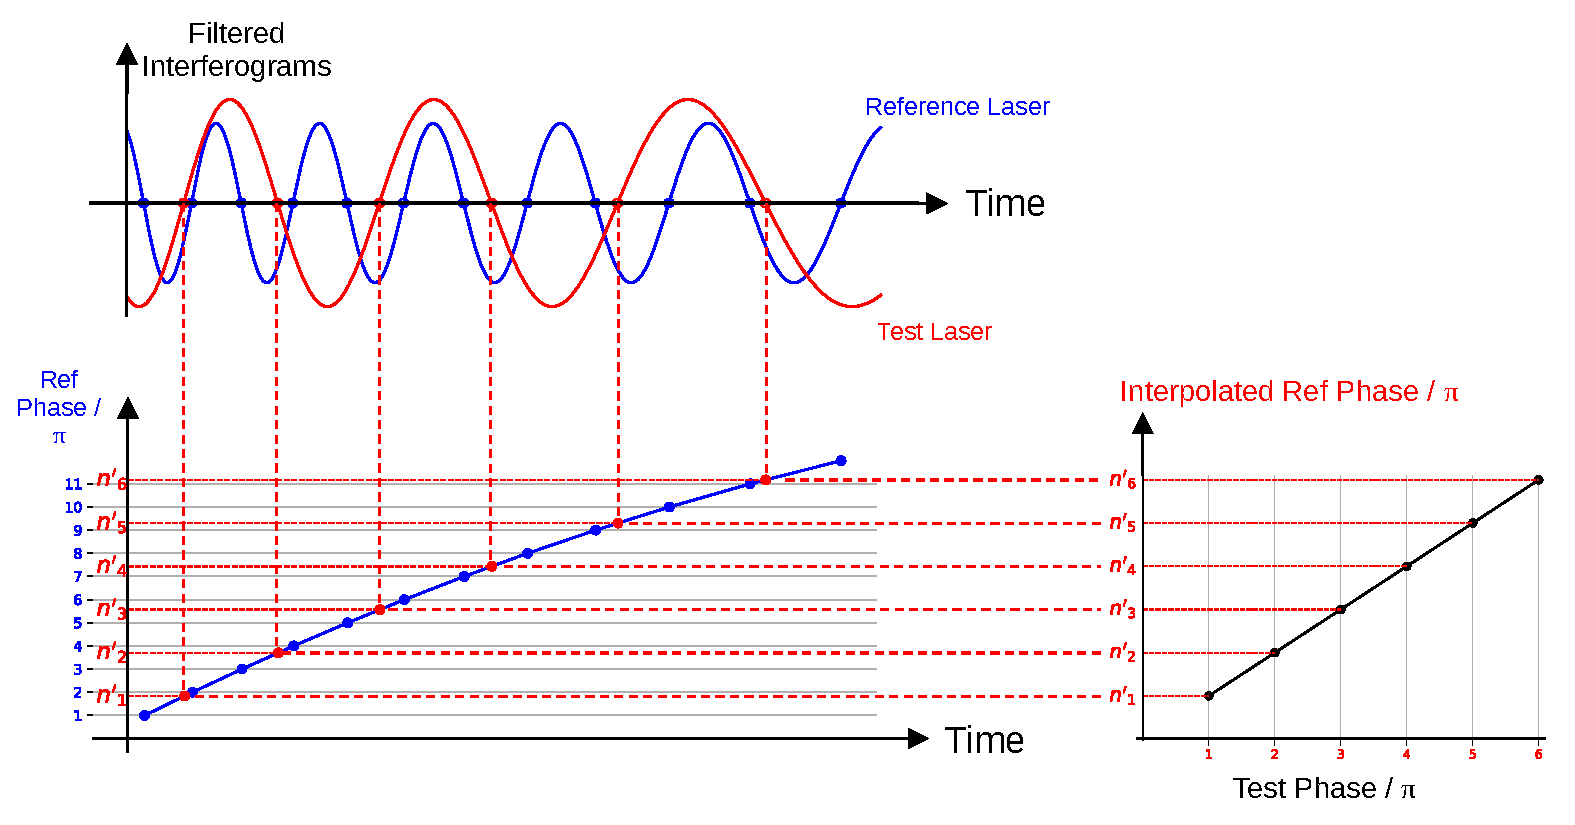
\includegraphics[width=1.0\linewidth]{diagrams/wl_phaseInterpolation}
	\caption{Diagram of procedure for the estimation of wavelength ratios optimized for digitally sampled interferograms. %The procedure does not require the storage of the entire waveform data, and can be evaluated in nearly real-time, up to the delay introduced by the interpolation stage.
	This diagram illustrates the procedure for estimating wavelength ratios optimized for digitally sampled interferograms. The blue curve in the lower left is constructed by plotting the cumulative number of reference zero-crossings against their respective timings. The timings of the test zero-crossings are then interpolated along this curve to determine $n'_j$, which represents the interpolated counting number of the $j^\mathrm{th}$ test zero-crossing. In the right pane, these values are plotted on the vertical against the test laser cumulative counting number. The slope of the resulting line gives the ratio of wavelengths.
	}
	\label{fig:wlphaseinterpolation}
\end{figure}

We can imagine this interpolation procedure pictorially by following Fig. \ref{fig:wlphaseinterpolation} as follows. We first construct a plot of the reference interferogram phase by marking the x-axis with the times of the zero crossings of the reference interferogram and the y-axis with the number of the zero crossing, incrementing by one each time a zero crossing is encountered. In the construction of Fig. \ref{fig:wlphaseinterpolation}, this is the blue plot in the lower-left pane. Then for each $i^\mathrm{th}$ zero crossing of the test laser interferogram, we interpolate this plot to find $n'_i$. As a concrete example, the value of $n'_3$ in Fig. \ref{fig:wlphaseinterpolation} is between 5 and 6.

We show explicitly this step as a linear interpolation. This interpolation step may be performed with higher order methods which consider many different points \cite{book_numerical_Press2007}, but for this application these methods seem to give little advantage over a simple linear interpolation. As depicted in Fig. \ref{fig:wllinearinterpolate}, for a zero crossing of the test laser interferogram occurring at a time $\tau_j$ between the zero crossing times $\tau^\mathrm{ref}_i$ and $\tau^\mathrm{ref}_{i+1}$ of the reference laser interferogram having numbers $n_i$ and $n_i + 1$, the interpolated zero crossing number is
\begin{equation}
	n'_j = \frac{\tau_j - \tau_i^\mathrm{ref}}{\tau_{i+1}^\mathrm{ref} - \tau_i^\mathrm{ref}} + n_i
\end{equation}

\begin{figure}[H]
	\centering
	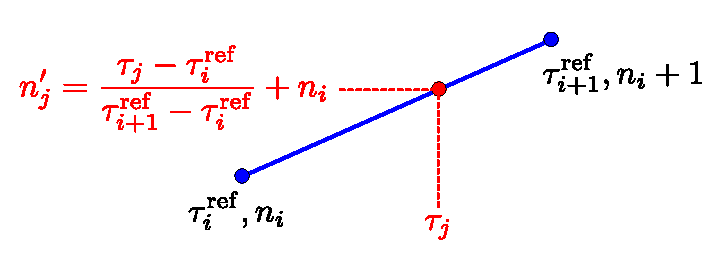
\includegraphics[width=0.5\linewidth]{diagrams/wl_linearInterpolate}
	\caption{Interpolation of the reference interferogram zero crossing times. This is depicted here as a simple linear interpolation, which is sufficient for interferogram oscillation frequencies which are far under the Nyquist value for the acquisition system. This interpolation stage determines how much of the interferogram waveform must be stored in memory at a particular time by the acquisition system.}
	\label{fig:wllinearinterpolate}
\end{figure}

\subsection{Slope Determination}
The final determination of wavelength is given by the slope of the linear fit which is made through the points in the lower-right of Fig. \ref{fig:wlphaseinterpolation}. This consists of the points \newline $(1, n'_1),\;(2, n'_2)\,\ldots\,(N, n'_N)$, where $N$ zero crossings of the test laser interferogram could be interpolated between crossings of the reference laser interferogram. The slope of the regression line is derived in the appendix and is given by equation (\ref{append_linreg_slope}), which simplifies using the known abscissa values
\begin{equation} \label{wl_wavelength_slope}
	\frac{\lambda}{\lambda_\mathrm{ref}} = 6\frac{
		(N+1)\sum_{j=1}^{N}n'_j - 2\sum_{j=1}^{N}jn'_j }{
		N(1-N^2)
	}
\end{equation}
This gives the wavelength ratio, as measured from the timing of the zero crossings of the filtered interferograms.

The analytical formulation in Eq. (\ref{wl_wavelength_slope}) allows the slope measurement to be conducted without the computational overhead of a general-purpose regression package, which would typically require the storage of all interpolated zero-crossing locations. Because this expression relies on the accumulation of weighted sums ($\sum n'_j$ and $\sum jn'_j$), the algorithm does not need to retain the history of every detected crossing in memory; instead, it only requires the storage of the current interpolated value and the running totals of these sums.

\subsection{Python Implementation of Fringe Counting Procedure}
We present a function here which computes the wavelength of a test laser from the two interferograms of the reference laser and test laser. For this, we need to know the wavelength of the reference laser. It is assumed that the two recordings have already been filtered such that their oscillations are centered on zero.

We require first a function which returns the zero crossings of a signal using the procedure depicted in Fig. \ref{fig:wlzerocross}. The zero crossings are returned as the abscissa coordinates.
\begin{lstlisting}[language=Python, basicstyle=\ttfamily\footnotesize]
import numpy as np

def getZeroCrossings(x, y):
    """
    Detect and interpolate the x-coordinates where the signal 'y' crosses
    zero.

    Parameters
    ----------
    x : array_like
        The independent variable (coordinates). Must be of the same length 
        as `y`.
    y : array_like
        The dependent variable (signal values) to be analyzed for zero
        crossings.

    Returns
    -------
    ndarray
        A 1D array containing the interpolated x-coordinates where the 
        signal 'y' crosses zero.

    Notes
    -----
    This function specifically detects "true" crossings (where the sign 
    actually flips). It does not explicitly handle cases where a data point 
    is exactly zero.

    Examples
    --------
    >>> x = np.array([0, 1, 2, 3, 4])
    >>> np.array([1, -1, -2, 3, 0.5])
    >>> getZeroCrossings(x, y)
    array([0.5, 2.4])
    """
    # Shift arrays to compare element i with i+1
    xi = np.array(x[0:-1])
    xi1 = np.array(x[1::])
    yi = np.array(y[0:-1])
    yi1= np.array(y[1::])

    # Identity sign changes
    mask = yi * yi1 < 0

    # Apply linear interpolation forumla to the selected indices
    xzero = -yi[mask] * (xi1[mask] - xi[mask]) /
            (yi1[mask] - yi[mask]) + xi[mask]

    return xzero
\end{lstlisting}

The wavelength determination is then performed using the function:
\begin{lstlisting}[language=Python, basicstyle=\ttfamily\footnotesize]
import numpy as np
from scipy.interpolate import interp1d
from numpy import polyfit

def wavelength(ref, sig, ref_wavelength_nm=632.991):
    """
    Calculate wavelength from two sampled interferograms of CW lasers.

    Parameters
    ----------
    ref : array_like
        Reference laser interferogram, stored as 1D array.
    sig : array_like
        Test laser interferogram, stored as 1D array. 
    ref_wavelength_nm : float, optional
        The known physical wavelength of the reference signal in nanometers. 
        Defaults to 632.991 (standard HeNe laser vacuum wavelength).

    Returns
    -------
    float
        The calculated wavelength scale factor for the input signal.

    Notes
    -----
    The hardcoded value 20 is used to avoid interpolation errors, 
    and corresponds to the number of reference zero crossings ignored to 
    ensure that we have encountered a zero crossing of the test laser.
    This number is exaggerated to account for possible transient edge effects.

    """
    # Generate Artificial Time Axis
    t=np.arange(len(ref))
    
    # Zero Crossing Times
    zc_ref = zeroCrossings(t, ref)
    zc_sig = zeroCrossings(t, sig)
    
    # Enumerate Zero Crossings
    n_ref = np.arange(len(zc_ref))
    n_sig = np.arange(len(zc_sig))
    
    # Interpolation
    ref_interp = interp1d(zc_ref, n_ref)
    
    # Linear Regression
    slope = polyfit(ref_interp(zc_sig[20:-20]), n_sig[20:-20], 1)[0]
    return ref_wavelength_nm/slope
\end{lstlisting}
Note that the hardcoded value \texttt{20} is used to avoid interpolation errors, and corresponds to the number of reference zero crossings ignored to ensure that we have encountered a zero crossing of the test laser. This number is exaggerated to account for possible transient edge effects.

\subsection{FPGA-Accelerated Acquisition Architecture}

The procedure described above can be evaluated in real time as the interferometer scans, providing a significant advantage for high-speed digital acquisition. This approach achieves the memory efficiency characteristic of simple fringe-counting methods, which compute only a ratio of total counts ($N_\mathrm{Ref}/N_\mathrm{Test}$), while providing vastly improved accuracy through the use of interpolated phase tracking and regression. By avoiding the need to store large waveform buffers, the algorithm is uniquely suited for integration into high-throughput, low-latency architectures.

In this work, the algorithm was implemented on a custom acquisition system based on a Red Pitaya single-board computer. This platform provides a high-performance environment for real-time signal processing, utilizing an on-board FPGA for high-speed data handling and a dual-channel, high-resolution ADC for the simultaneous capture of the reference and test laser interferograms. Crucially, the summation of the weighted sums is performed directly within the FPGA fabric. To prevent overflow and maintain numerical integrity during long scans, these accumulations are implemented using 128-bit integer counters (this precision remains highly configurable) synchronized to the 125 MHz ADC clock. These extended-precision integer sums are then transferred to the operating system via block memory generators, where the final conversion to floating-point representation and subsequent scaling are performed in the software layer.

\section{Python Implementation of Linear Least Squares Fitting}
For large datasets, evaluation of the pseudoinverse formula $(A^T A)^{-1}A^T \vec{b}$ used in (\ref{leastSquares}) and (\ref{append_leastSquares}) can be numerically unstable and costly if the inverse is computed directly. Moreover, the formation of $A^T A$ can lead to a matrix which is ill-conditioned, leading to large roundoff errors and unstable inversion.

In this work, we make use of the NumPy library \cite{numpy_citation}, which has become a standard tool in data analysis with the Python programming language. Modern packages such as \newline \texttt{numpy.linalg.lstsq} avoid some of the numerical instabilities of evaluating the pseudoinverse by using matrix factorization methods \cite{LAPACK}.

The following is a function for performing fitting to $x$-$y$ data of an equation having the form (\ref{append_basis_combo}), given again here
\begin{equation*}
    f(x) = c_1 f_1(x) + c_2 f_2(x) + \ldots + c_n f_n(x)
\end{equation*}
This form is a linear combination of basis functions $f_{1\ldots n}(x)$. The function given here returns the set of coefficients $c_{1\ldots n}$ which fit the above function to the data.

Within the function, the $A$ matrix entries are scaled between $[0,1]$. This ensures that the numerical scale of the pseudoinverse computation is decoupled from the scales of the resulting concentration numbers. This can help to improve accuracy of the floating point operations within the computation.

\begin{lstlisting}[language=Python, basicstyle=\ttfamily\footnotesize]
import numpy as np

def fitScales(data, basisFunctions, weights=None):
    """
    Perform a weighted least-squares fit of coefficients for
    a given set of basis functions.

    This function solves the linear least-squares problem: 
    min ||W * (A*c - b)||^2, where A is the matrix of basis
    functions evaluated at the provided data points.
    Transparent normalization is performed to improve
    numerical stability during the inversion process.

    Parameters
    ----------
    data : tuple of (ndarray, ndarray)
        A tuple containing:
        * data[0] (ndarray): x-coordinates/input.
        * data[1] (ndarray): y-coordinates/target.
    basisFunctions : list of callable
        A list of functions where each function `f` takes a single input 
        and returns a value (or array) corresponding to the basis 
        expansion at that point.
    weights : ndarray, optional
        An array of weights applied to the design matrix and target vector. 
        Must be broadcastable to the shape of the evaluated basis functions. 
        If None (default), all points are weighted equally.

    Returns
    -------
    ndarray
        A 1D array of fitted coefficients (the 'res' vector) scaled back 
        to the original magnitude.
    """
    # Prepare the data, apply weighting if given
    A = [f(data[0]) for f in basisFunctions]
    if(weights is not None):
        A = np.multiply(weights, A)
        b = [ np.multiply(weights, data[1]) ]
    else:
        b=[data[1]]
    A = np.transpose(A)
    b = np.transpose(b)

    # Scale A by its maximum value for numerical stability
    norm = np.max(A)
    A = A / norm

    # Peform the solution of the over-determined system
    res = np.linalg.lstsq(A, b, rcond=None)[0]

    # Return the solution, scaled to the original coordinates
    return (res / norm).flatten()
\end{lstlisting}

Computation of the pseudoinverse matrix $M = (A^T A)^{-1}A^T$ used in (\ref{error_conc_alpha}) and (\ref{append_leastSquares}) can be performed using the following function. The pseudoinverse is constructed column-by-column by solving the least-squares problem for each unit vector.

\begin{lstlisting}[language=Python, basicstyle=\ttfamily\footnotesize]
def getMatrixM(x_arr, basisFunctions, weights=None):
    """
    Compute the pseudoinverse matrix (Moore-Penrose) for a given basis 
    expansion using a stabilized least-squares approach.

    The function computes the matrix $M$ such that it acts as the 
    pseudoinverse of the design matrix $A$. To ensure numerical stability, 
    the design matrix is scaled by its maximum element before computation 
    and unscaled after.

    Parameters
    ----------
    x_arr : ndarray
        The independent variable (input coordinates) at which to 
        evaluate the basis functions.
    basisFunctions : list of callable
        A list of functions where each function `f` takes a single input 
        and returns a value (or array) corresponding to the basis 
        expansion at that point.
    weights : ndarray, optional
        An array of weights applied to the design matrix rows. 
        Must be broadcastable to the shape of the evaluated basis functions. 
        If None (default), all points are weighted equally.

    Returns
    -------
    ndarray
        The pseudoinverse matrix M
    """

    A = [f(x_arr) for f in basisFunctions]
    if(weights is not None):
        A = np.multiply(weights, A)
    A = np.transpose(A)
    norm = np.max(A)
    A = A/norm

    M = []
    for i in range(A.shape[0]):
        unitVect = np.zeros(A.shape[0])
        unitVect[i] = 1.0
        res = np.linalg.lstsq(A, unitVect, rcond=None)
        M.append(res[0]/norm)
    M = np.transpose(M)
    return M
\end{lstlisting}

The following function is a wrapper function which computes explicitly the formula (\ref{error_conc_alpha}), given the standard deviations of the absorption measurements.

\begin{lstlisting}[language=Python, basicstyle=\ttfamily\footnotesize]
def getFitErrors(x_arr, basisFunctions, stds, weights=None):
    """
    Calculate the propagated standard deviations of the fitted coefficients.

    Parameters
    ----------
    x_arr : ndarray
    The independent variable (input coordinates) used to evaluate 
    the basis functions.
    basisFunctions : list of callable
    A list of functions where each function `f` takes a single input 
    and returns a value/array at that point.
    stds : ndarray
    An array of standard deviations (uncertainties) corresponding to 
    each data point in the input set. Must have the same length as `x_arr`.
    weights : ndarray, optional
    An array of weights applied during the matrix computation. 
    Must be broadcastable to the shape of the evaluated basis functions.

    Returns
    -------
    ndarray
    A 1D array of size `Nr` (number of basis functions) containing 
    the propagated standard deviation for each coefficient.
    """

    # Retrieve the pseudoinverse matrix M
    M = getMatrixM(x_arr, basisFunctions, weights=weights)
    # Nr: Number of basis functions, Nc: Number of data points
    Nr, Nc = M.shape

    errs = np.zeros(Nr)

    # Propagation of error formula: sum of (weight * uncertainty)^2
    # Here M[i,j] acts as the sensitivity coefficient
    for i in range(Nr):
        for j in range(Nc):
            errs[i] = errs[i] + M[i, j]**2 * stds[j]**2

        # Take square root to convert variance back to standard deviation
        errs[i] = np.sqrt(errs[i])

    return np.array(errs)

\end{lstlisting}

\section{Rapid Fitting of Cavity Ringdown Recordings} \label{sec:subsys_rapidLMfit}
The typical approach of determining the ringdown time of a cavity is to fit the exponentially decaying optical signal using a nonlinear fitting method. Such methods can be costly in terms of computational time and complexity, especially when implemented from a general fitting package. While methods have been presented which enable rapid ringdown time estimation \cite{crds_freq_domain, frontiers_mol_spec}, these always involve some trade-off in the accuracy of the retrieved fit. An exception can be made for recently investigated neural-network based fitting routines \cite{crds_ringdownFit_neuralNet}

In this section, we present formulas for the rapid evaluation of the Levenberg-Marquardt algorithm in the specialized case of the exponential decay model with an undermined offset. This is combined with a robust procedure for construction of an initial guess. The combination of these two optimizations gives a fitting procedure which always converges with a fixed number of iterations with few exceptions.

It is a simple matter to extract the ringdown time from a signal of the type
\begin{equation}\label{noOffsetModel}
	f(t) = A e^{-t/\tau}
\end{equation}
This can be done by fitting the slope of $\log f$ plotted against time. However, this procedure breaks down as soon as a simple DC offset is added to the signal
\begin{equation}\label{model}
	f(t) = A e^{-t/\tau} + B
\end{equation}

\subsection{Levenberg-Marquandt Algorithm for Exponential Decay with Offset}

The Levenberg-Marquandt algorithm is a nonlinear iterative algorithm for finding a set of parameters that make a model equation fit a set of data points by the least total squared residual. %In order for the algorithm to converge to a fit in a small number of steps, a good initial guess for the fit parameters is needed. Using the algorithm in section \ref{fpgaAlg}, we can come up with a set of good initial parameters that can allow the Levenberg-Marquandt algorithm to converge in a fixed number of iterations.

Let us define a model function $f(t;\; \vec{\beta} )$ containing the set of parameters given by the vector $\vec{\beta}$. For an initial guess of the parameters $\vec{\beta_0}$, we can retrieve a refined set of parameters
\begin{equation}\label{lmfit_iterationEqn}
	\vec{\beta} = \vec{\beta_0} + \vec{\delta}
\end{equation}
that is given by the gradient descent of the least squares weighting function. The change to the parameters $\vec{\delta}$ is given by solving the matrix equation
\begin{equation}\label{lmfit_matrixSolve}
	\left[ J^T J + \lambda\cdot\text{diag}\left( J^T J \right) \right] \vec{\delta} = J^T \left[\vec{y} - \vec{f}(\vec{\beta}) \right]
\end{equation}
Here $\lambda$ is a damping factor that controls speed of convergence and overshoot. The matrix $J$ is the Jacobian of the model function, defined by
\begin{equation}
	\vec{J_i} = \frac{\partial \vec{f}(t_i,\vec{\beta})}{\partial \vec{\beta}}
\end{equation}

This process is repeated until convergence is obtained. For the specific case of the model function in (\ref{model}), we have the following components for $J$

\begin{eqnarray}
	\vec{J_A} &= \frac{\partial \vec{f}}{\partial A} &= e^{-\vec{t}/\tau} \\
	\vec{J_B} &= \frac{\partial \vec{f}}{\partial B} &= \vec{1} \\
	\vec{J_\tau} &= \frac{\partial \vec{f}}{\partial \tau} &= A\frac{\vec{t}}{\tau^2}e^{-\vec{t}/\tau} 
\end{eqnarray}

Substituting these, we obtain the following for the left hand side of equation (\ref{lmfit_matrixSolve})

\begin{equation*}
	%\begin{pmatrix}
	%	\vec{J_A} \cdot \vec{J_A} & \vec{J_A} \cdot \vec{J_B} & \vec{J_A} \cdot \vec{J_\tau} \\ 
	%	\vec{J_B} \cdot \vec{J_A} & \vec{J_B} \cdot \vec{J_B} & \vec{J_B} \cdot \vec{J_\tau} \\ 
	%	\vec{J_\tau} \cdot \vec{J_A} & \vec{J_\tau} \cdot \vec{J_B} & \vec{J_\tau} \cdot \vec{J_\tau}
	%\end{pmatrix} \vec{\delta}
	%+ \lambda\cdot\text{diag}\left( J^T J \right)\vec{\delta}
	%=
	\begin{pmatrix}
		(1+\lambda)s_2 & s_1 & \frac{A}{\tau^2}s_4 \\ 
		s_1 & (1+\lambda)N & \frac{A}{\tau^2}s_3 \\ 
		\frac{A}{\tau^2} & \frac{A}{\tau^2}s_3 & \frac{A^2}{\tau^4}(1+\lambda)s_5
	\end{pmatrix} \vec{\delta}
\end{equation*}

For simplicity of notation, we have defined the following sums which can be evaluated analytically using the fact that the values of $t_n$ are known from the sampling time $t_s$ as $t_n = n t_s$. Using the definition $R \equiv e^{-t_s/\tau}$, the sums over the $N$ number of samples is carried out with $n=1\ldots N-1$
\begin{eqnarray}
	s_1 &= \sum_n e^{-t_n/\tau} &= \frac{1-R^N}{1-R} \\
	s_2 &= \sum_n e^{-2t_n/\tau} &= \frac{1-R^{2N}}{1-R^2} \\
	s_3 &= \sum_n t_n e^{-t_n/\tau} &= t_s \frac{R - N R^N + (N-1) R^{N+1}}{(1-R)^2} \\
	s_4 &= \sum_n t_n e^{-2t_n/\tau} &= t_s \frac{R^2 - NR^{2N} + (N-1) R^{2N+2}}{(1-R^2)^2} \\
	s_5 &= \sum_n t_n^2 e^{-2t_n/\tau} &= t_s^2 \frac{-R^2 - R^4 +N^2R^{2N} + (1+2N-2N^2)R^{2+2N}+(N-1)^2 R^{4+2N}}{(R^2-1)^3} \nonumber \\
\end{eqnarray}

The right hand side of equation (\ref{lmfit_matrixSolve}) can then be seen to be equal to

\begin{equation}
	\begin{pmatrix}
		\vec{J_A}^T \\ 
		\vec{J_B}^T \\ 
		\vec{J_\tau}^T
	\end{pmatrix}
	\left(\vec{y} - \vec{f}(\beta) \right) 
	=
	\begin{pmatrix}
		r_1 - A s_2 - B s_1 \\ 
		r_2 - A s_1 - B N \\ 
		\frac{A}{\tau^2}\left( r_3 -A s_4 - B S_3 \right)
	\end{pmatrix} 
\end{equation}
Here we have defined the following sums which must be evaluated on the data points.
\begin{align}
	r_1 = \sum_n y_n e^{-t_n/\tau} &&
	%r_1 = \sum_n y_n R^n &&
	r_2 = \sum_n y_n &&
	r_3 = \sum_n t_n y_n e^{-t_n/\tau}
\end{align}

In terms of these variables, the components of $\vec{\delta}$ can be solved for. We then have the explicit expressions for how the parameters $A$, $B$, and $\tau$ are updated for each iteration of the algorithm	
\begin{align}
	\delta_A &=\frac{r_1(s_3^2 -N(1+\lambda)^2 s_5) + r_2 (-s_3 s_4 + (1+\lambda) s_1 s_5) + r_3 \frac{\tau^2}{A}(-s_1 s_3 + (1+\lambda)N s_4)}{s_2(1+\lambda)\left[(1+\lambda)^2 N s_5 - s_3^2 \right] + s_1 \left[-s_1 s_5 (1+\lambda) + s_3 s_4 \right] + s_4\left[ s_1 s_3 - (1 + \lambda)N s_4\right]} \\
	\delta_B &= \frac{r_1(-s_3s_4 +(1+\lambda)s_1s_5) + r_2 (s_4^2 - (1+\lambda)^2 s_2 s_5) + r_3 \frac{\tau^2}{A}(-s_1 s_4 + (1+\lambda)s_2 s_3)}{s_2(1+\lambda)\left[(1+\lambda)^2 N s_5 - s_3^2 \right] + s_1 \left[-s_1 s_5 (1+\lambda) + s_3 s_4 \right] + s_4\left[ s_1 s_3 - (1 + \lambda)N s_4\right]} \\
	\delta_\tau &=\frac{\tau^2}{A} \frac{r_1(-s_1s_3 +(1+\lambda)Ns_4) + r_2 (-s_1s_4 + (1+\lambda)^2 s_2 s_3) + r_3 \frac{\tau^2}{A}(s_1^2 - (1+\lambda)^2N s_2)}{s_2(1+\lambda)\left[(1+\lambda)^2 N s_5 - s_3^2 \right] + s_1 \left[-s_1 s_5 (1+\lambda) + s_3 s_4 \right] + s_4\left[ s_1 s_3 - (1 + \lambda)N s_4\right]}
\end{align}

Since the $s_i$ terms can be evaluated analytically, only the $r_i$ sums need to be calculated for each iteration of the algorithm. Now we have for an initial guess for the parameters $A$, $B$, $\tau$, a solution for how these parameters should be changed to optimize the fit to the data.

\subsection{Finding an Initial Guess}
The real-time performance of the nonlinear fitting routine can be drastically improved with an initial guess which is already close to the optimized parameters. We describe here a robust method for obtaining such an initial guess. This method requires two passes through the captured data; the first pass gives an estimate of the ringdown time and can be evaluated in parallel with the data acquisition itself, while the second pass gives an estimate for the $A$ and $B$ coefficients.

\subsubsection{Ringdown time estimate}
The ringdown time can be determined from the Fourier coefficients of the captured signal in a manner similar to that which is used in \cite{crds_freq_domain}. We define the quantities $S_n$ and $C_n$ by the following Fourier integrals of the signal
\begin{align}
	S_n \equiv \int_{0}^{T}y(t) \sin \left(\frac{2\pi n t}{T}\right)\, dt
	\qquad\qquad\qquad
	C_n \equiv \int_{0}^{T}y(t) \cos \left(\frac{2\pi n t}{T}\right)\, dt
\end{align}
If the photodetector signal $y(t)$ is well modeled by the function $f(t)$, then using a simple integration by parts
\begin{equation}
	C_n = \int_0^T e^{-t/ \tau} \cos \left( \frac{2 \pi n t}{T} \right) dt
	=
	\cancel{\frac{2 \pi n}{T}  e^{-t/ \tau} \sin \left( \frac{2 \pi n t}{T} \right) \Biggr|_0^T} +
	\frac{1}{\tau} \frac{T}{2 \pi n}  \int_0^T e^{-t/ \tau} \sin \left( \frac{2 \pi n t}{T} \right) dt
\end{equation}
we see that the sine integrals $S_n$ are related to the cosine integrals $C_n$ by the relation
\begin{equation}
	\frac{S_n}{C_n} = \frac{2\pi \tau}{T} n
\end{equation}
By evaluating the ratio $S_n/C_n$ for several values of $n>0$, a straight line can be constructed by plotting the ratio $S_n/C_n$ against the harmonic number $n$. \textit{The slope of this line then gives the ringdown time} $\tau$ since the observation period $T$ is known and chosen beforehand.

For $n>0$, the $S_n$ and $C_n$ have no contribution from the DC term in the photodetector signal $B$. It is clear that this method is immune to the signal offset.

\subsubsection{Estimate of the $A$ and $B$ coefficients}
Once a guess for the ringdown time $\tau$ is obtained by the above Fourier method, the two component linear decomposition formulas in (\ref{append_lsq_two_comp}) can be directly used to obtain the scale coefficients $A$ and $B$ with the substitutions $f_1(t) = e^{-t/\tau}$ and $f_2(t) = 1$.

All three dot-product combinations of the two basis functions are easily computed analytically
\begin{align}
	a_{11} = R^2 \frac{1 - R^{2N}}{1-R^2} && a_{22} = N && a_{12} = R \frac{1 - R^N}{1 - R} &&\text{where}&& R \equiv e^{-t_s/\tau}
\end{align}
In the above expressions $t_s$ is the sampling time of the ringdown signal, which is composed of the samples $\left\{y_1\; y_2\;\ldots\; y_N\right\}$. These samples enter into the initial guess formation procedure through the sums
\begin{align}
	\bar{a}_1 = \sum_{n=1}^{N} y_n e^{-nt_s/\tau} && \bar{a}_2 = \sum_{n=1}^{N} y_n
\end{align}
Once the above quantities have been computed using our initial estimate for the ringdown time $\tau$, we can then write the initial guess for the $A$ and $B$ coefficients as
\begin{align}
	A = \frac{a_{22} \bar{a}_1 - a_{12}\bar{a}_2}{a_{11}a_{22} - a_{12}^2}
	&&
	B = \frac{a_{11} \bar{a}_2 - a_{12}\bar{a}_1}{a_{11}a_{22} - a_{12}^2}
\end{align}

The above procedure for finding the initial guess for $A$ and $B$ only requires a single parse through the data. Since we require beforehand an estimate of $\tau$, this cannot be evaluated simultaneously with the data acquisition.

%\subsection{Fitting on a Deadline -- Implementation in Real-Time Acquisition System}

\section{Implementation of the Acetone Cross Section in Computer Code} \label{sec:subsys_acetone_function}
The following function gives the fitted function describing the NIR acetone cross section. This function is plotted in Fig. \ref{fig:acetone_broadband_superfit}, and the hard-coded values used are given in Table \ref{tbl:acetone_broadband_coeffs} and Table \ref{table:acetone_coeffs}. The following code is given in the Python programming language.

\subsection{Acetone NIR Cross Section}
Reported in this section is a Python function for easily evaluating the acetone cross section model which was presented in Sec. \ref{sec:acetone_broadband} and Eq. (\ref{acetone_super_model}). The hard-coded coefficients are the fit coefficients presented in Table \ref{tbl:acetone_broadband_coeffs}. Included is a helper function \texttt{gauss(x, c[0], c[1], c[2])} which is used to evaluate a single Gaussian peak. The asymmetric peak function (\ref{sigma_tilde}), along with some of the coefficients of Table \ref{table:acetone_coeffs} are also used.

\begin{lstlisting}[language=Python, basicstyle=\ttfamily\footnotesize]
import numpy as np

def gauss(x, A, x0, w):
    """
    Compute the Gaussian function for a single peak.

    Parameters
    ----------
    x : ndarray
        The spectral coordinate array (wavelength in nm).
    A : float
        Amplitude of the peak.
    x0 : float
        The center position of the peak.
    w : float
        The width parameter (standard deviation/scale) of the Gaussian.
    
    Returns
    -------
    ndarray
        The evaluated Gaussian function at points x.
    """
    return A*np.exp(-(x-x0)**2/w**2)

def acetone_NIR_xs(x):
    """
    Calculate the absorption cross-section of Acetone in the NIR spectrum.

    This function computes the total absorption cross-section by summing 
    a series of Gaussian absorption lines and adding a specific 
    asymmetric feature (modeled via an arctan/Lorentzian-style term). 

    Parameters
    ----------
    x : ndarray
        The spectral coordinate array (wavelength in nm) at which to 
        evaluate the cross-section.

    Returns
    -------
    ndarray
        The calculated absorption cross-section values in units of cm^2, 
        with the same shape as the input `x`.
    """
    # Empirical constants for the asymmetric feature
    p0 = 0.70523665       # The stationary Lorentzian component (nm)
    p1 = 3.30411644e-01   # The local asymmetry of the peak
    p2 = 1672.4421        # Center of the asymmetric feature (nm)
    p3 = 3.39664499e-01   # Clamping term (nm)
    d1 =  4.07793263e-22  # Amplitude of asymmetric peak (cm^2)
    d0 = -3.61813970e-24  # Constant offset term (cm^2)

    # Gaussian peak parameters: [Amplitude, Center, Width]
    cg =  [ [1.35986073e-23, 1.60825527e+03, 1.70398884e+01],
            [1.19850011e-22, 1.65089421e+03, 1.73307837e+01],
            [7.74849891e-24, 1.65172811e+03, 4.22113059e-01],
            [3.83851582e-22, 1.66898148e+03, 2.89021701e+00],
            [2.17705109e-22, 1.66775570e+03, 5.41898839e+00],
            [2.32033931e-23, 1.67044823e+03, 5.15654864e-01],
            [6.77081682e-22, 1.67519932e+03, 5.02332894e+00],
            [5.40555517e-22, 1.68828973e+03, 5.47489581e+00],
            [2.39423927e-23, 1.69132528e+03, 5.43943755e-01],
            [2.71987962e-22, 1.69494138e+03, 4.09722699e+00],
            [5.09704537e-22, 1.70687072e+03, 2.63261427e+01],
            [7.91604650e-22, 1.73391534e+03, 1.39920104e+01],
            [9.21396457e-23, 1.75763838e+03, 5.57521753e+00],
            [3.13335887e-22, 1.77522543e+03, 1.18572793e+01],
            [2.53193043e-23, 1.84785802e+03, 7.63312916e+00],
            [1.91223143e-22, 1.93687181e+03, 1.37439004e+01] ]

    out = np.zeros_like(x)

    # Sum the Gaussian components
    for ci in cg:
        out = out + gauss(x, *ci)
    
    # Calculate the gamma term, and add the asymmetric peak
    gamma = p0 + p1*p3*np.arctan((x-p2)/p3)
    out = out + d1*gamma**2/((x-p2)**2 + gamma**2)
    
    # Return the sum, plus a constant offset
    return out + d0
\end{lstlisting}
The above function is easily plotted using the Matplotlib library and supports vector inputs. This is shown using the following lines of Python:
\begin{lstlisting}[language=Python, basicstyle=\ttfamily\footnotesize]
import matplotlib.pyplot as plt

x = np.linspace(1600, 2000, 10_000)
y = acetone_NIR_xs(x)

plt.plot(x, y)

plt.xlabel("Wavelength [nm]")
plt.ylabel("Cross Section [cm$^2$]")
\end{lstlisting}


\chapter{MATHEMATICAL DERIVATIONS}

\section{Wavelength Measurement with a Michelson Interferometer} \label{sec:wl_wavelength}
This section describes the precise measurement of wavelength ratios using the configuration of a scanning Michelson interferometer, as well as details a specialized digital algorithm designed to extract these ratios with high stability. By leveraging high-resolution phase tracking and hardware-accelerated regression, we present a method that maintains extreme precision even in the presence of non-uniform mechanical motion of the apparatus.

The basic configuration for a Michelson interferometer is shown in Fig. \ref{fig:wl_michelsonsimple}, consisting of one fixed arm having length $D$ and another movable arm having length $D + d$. Incoming light is split into two paths using a beam splitter. These two paths traverse twice the two arms of the interferometer, and are recombined using the same beam splitter onto a photodetector.
\begin{figure}[H]
	\centering
	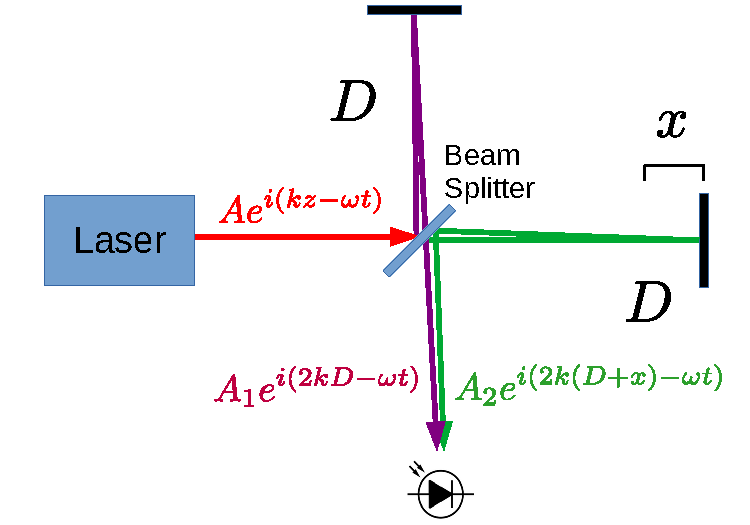
\includegraphics[width=0.5\linewidth]{diagrams/wl_michelsonSimple}
	\caption{A simplified configuration of a scanning Michelson interferometer. A beam is split into two paths (shown in green and purple) by a beam splitter. The path shown in purple traverses a distance of $2D$, while the green beam travels a length $2(D+x)$ before being recombined at the beam splitter. Due to the time varying delay between the beams, a sinusoidal pattern in time is observed on the photodetector.}
	\label{fig:wl_michelsonsimple}
\end{figure}

The incoming electric field can be described using the phasor
\begin{equation}
	E_\mathrm{in} = A e^{i(kz - \omega t)}
\end{equation}
After traversing the fixed arm for a total distance of $2D$, the contribution of light at the output of the beam splitter from this path is
\begin{equation}
	E_1 = A_1 e^{i(2kD - \omega t)}
\end{equation}
while the other path gives the contribution
\begin{equation}
	E_2 = A_2 e^{i(2k(D+x) - \omega t)} = A_2 e^{2ikx}e^{i(2kD - \omega t)}
\end{equation}
The photodetector is exposed to the sum of the two fields
\begin{align}
	E_p = E_1 + E_2 %&= A_1 e^{i(2kD - \omega t)} + A_2 e^{2ikd}e^{i(2kD - \omega t)} \\
	&= \left(A_1 + A_2 e^{2ikx}\right)e^{i(2kD - \omega t)}
\end{align}

It is clear that the field at the detector depends directly on the optical path difference (OPD) by the relation to the translation stage movement $\delta = 2x$ which is particular to the mechanical configuration of the delay. Proceeding forward, we use the OPD $\delta$ as it is independent of the particular mechanical configuration of the interferometer used to create the delay. The photodetector does not respond to the rapidly oscillating electric field, but to the time-averaged intensity, so the signal from the photodetector is proportional to
\begin{align}
	I_p(\delta) = E_p^*E_p &= \left(A_1 + A_2 e^{ik\delta}\right)\left(A_1^* + A_2^* e^{-ik\delta}\right) \\
	&= \left|A_1\right|^2 + \left|A_2\right|^2 + A_1A_2^*e^{-ik\delta} + A_1^*A_2e^{ik\delta}
\end{align}
The coefficients $A_{1,2}$ are in general complex and when written in the polar form $A_{1,2} = \left|A_{1,2}\right| e^{i\phi_{1,2}}$ the $\phi_{1,2}$ represent a constant phase shift of the output fields relative to the input field. Dropping the absolute value and writing the phase shift explicitly, the light intensity at the detector becomes
\begin{equation}\label{wl_sig_monochromatic}
	I_p(\delta) = A_1^2 + A_2^2 + A_1A_2\cos(k\delta + \phi_2 - \phi_1)
\end{equation}
The intensity detected by the photodetector is an offset sinusoidal function of the OPD $\delta$. The amplitude of this sinusoid is maximized when the beams emerging from each arm have the same field strength (or equivalently the same intensity) which occurs when $A_1 = A_2$.

\section{The Beer-Lambert law}
When light propagates through an opaque medium, some of the light is absorbed and the transmitted intensity is lowered. For now we will assume the light is monochromatic, but we can later relax this assumption using the superposition principle.

Consider a simple absorbing medium which is thin and has small completely opaque centers distributed throughout. It is clear that the change in light intensity $\Delta I$ which would be observed on the other side is proportional to the incident intensity $I$, since the transmitted intensity only consists of the locations where a "shadow" is not cast into the beam.

\begin{figure}[H]
	\centering
	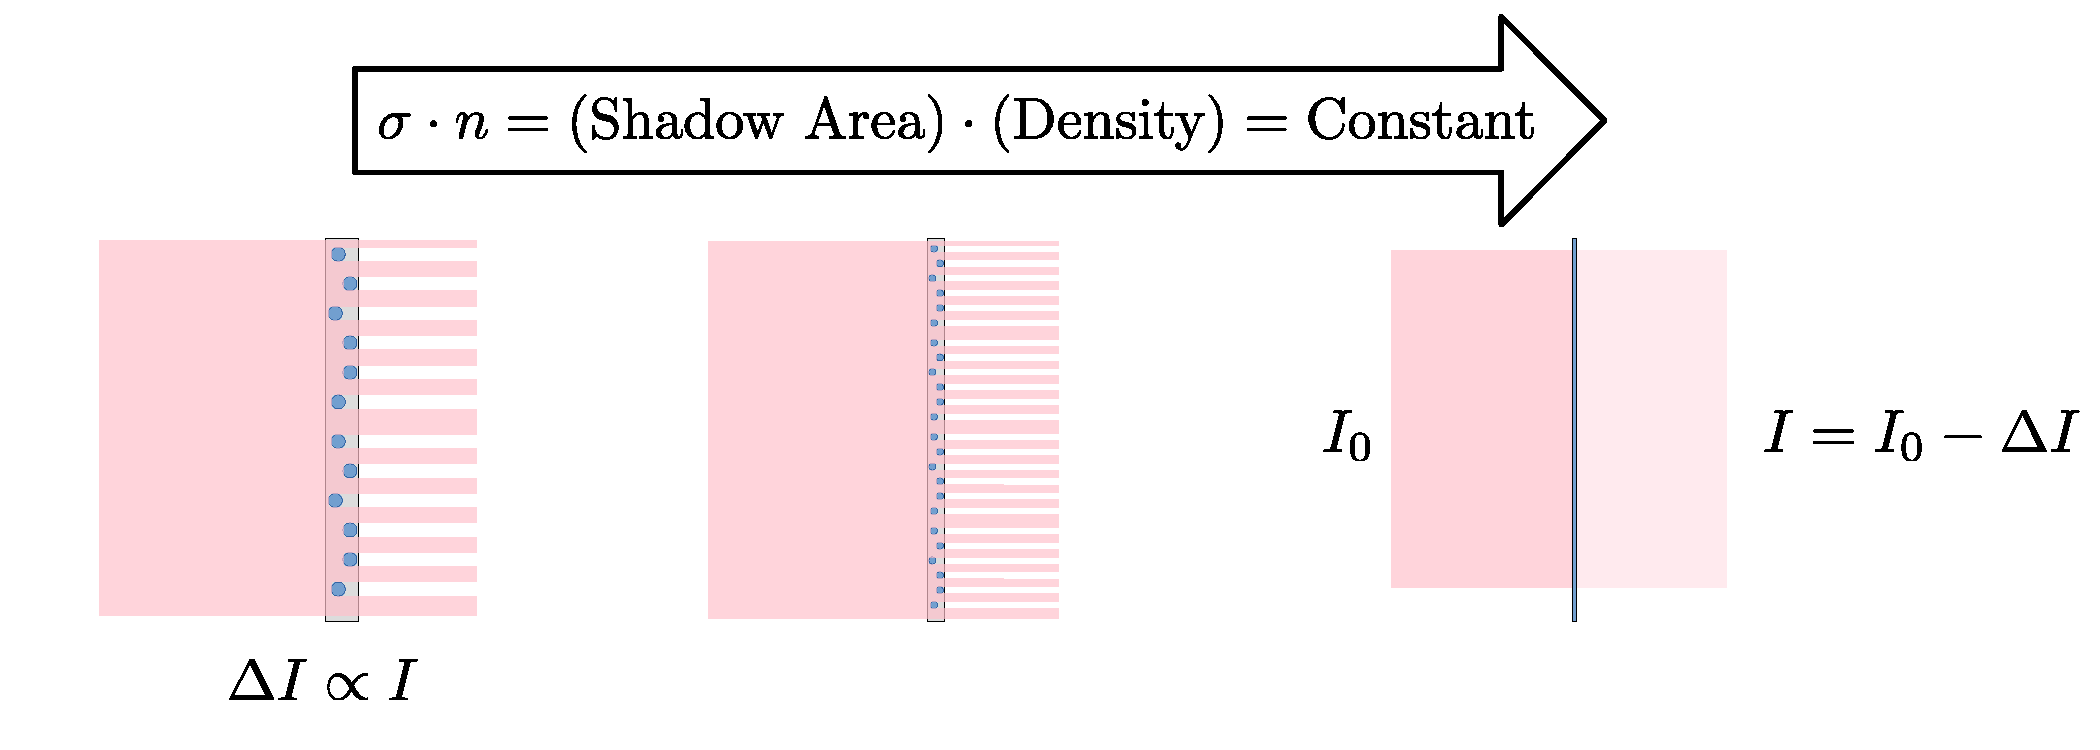
\includegraphics[width=0.9\linewidth]{diagrams/absorption_prop}
	\caption{Characterizing a material with a model of small opaque absorbing centers. The light transmitted through the material is the light that is not blocked by these objects. The change in light intensity $\Delta I$ is therefore proportional to the incident light intensity $I_0$. Depicted is the limiting process of scaling down the cross sectional area while increasing the particle density. If the same change in light intensity $\Delta I$ is to remain constant, then the product of the cross sectional area of the absorbing particles and their density must remain constant as we proceed to a thin slab.}
	\label{fig:absorption_prop}
\end{figure}

We make the assumption that thin slabs of absorbing material act independently in the sense that the change in intensity through each slab only depends on the incident intensity $\Delta I \propto I$. This would not be the case for the exaggerated case depicted in the left of Fig. \ref{fig:absorption_prop} since if an identical slab was placed in the transmitted beam path then the shadow cast by the first absorbing centers would coincide with the locations of the centers in the second slab. If we assume that these centers are randomly and homogenously distributed throughout the medium then this dependence is removed. Additionally due to the wave nature of light, the effect of coinciding shadows would be reduced by diffraction.

We can see from Fig. \ref{fig:absorption_prop} that if we shrink these small absorbing centers as we shrink the width of the slab, then there is a decreasing probability of overlapping shadows with a subsequent slab. In the limit of small scattering centers and a homogeneous distribution, the thin slabs of absorbing material behave independently of each other.

For a medium of thickness $L$, we can subdivide this length into $N$ small slices of thickness $\Delta x = L/N$ as in Fig. \ref{fig:absorption_slabs}. For a thin slice, we can presume that the change in light intensity $\Delta I$ transmitted through a small slice is proportional to the incident light intensity and the thickness of the slab. The constant of proportionality $\alpha$ characterizes the interaction of the material with the particular wavelength of light.

\begin{equation}\label{_beerDiff}
	\Delta I = - \alpha I \Delta x
\end{equation}

\begin{figure}[H]
	\centering
	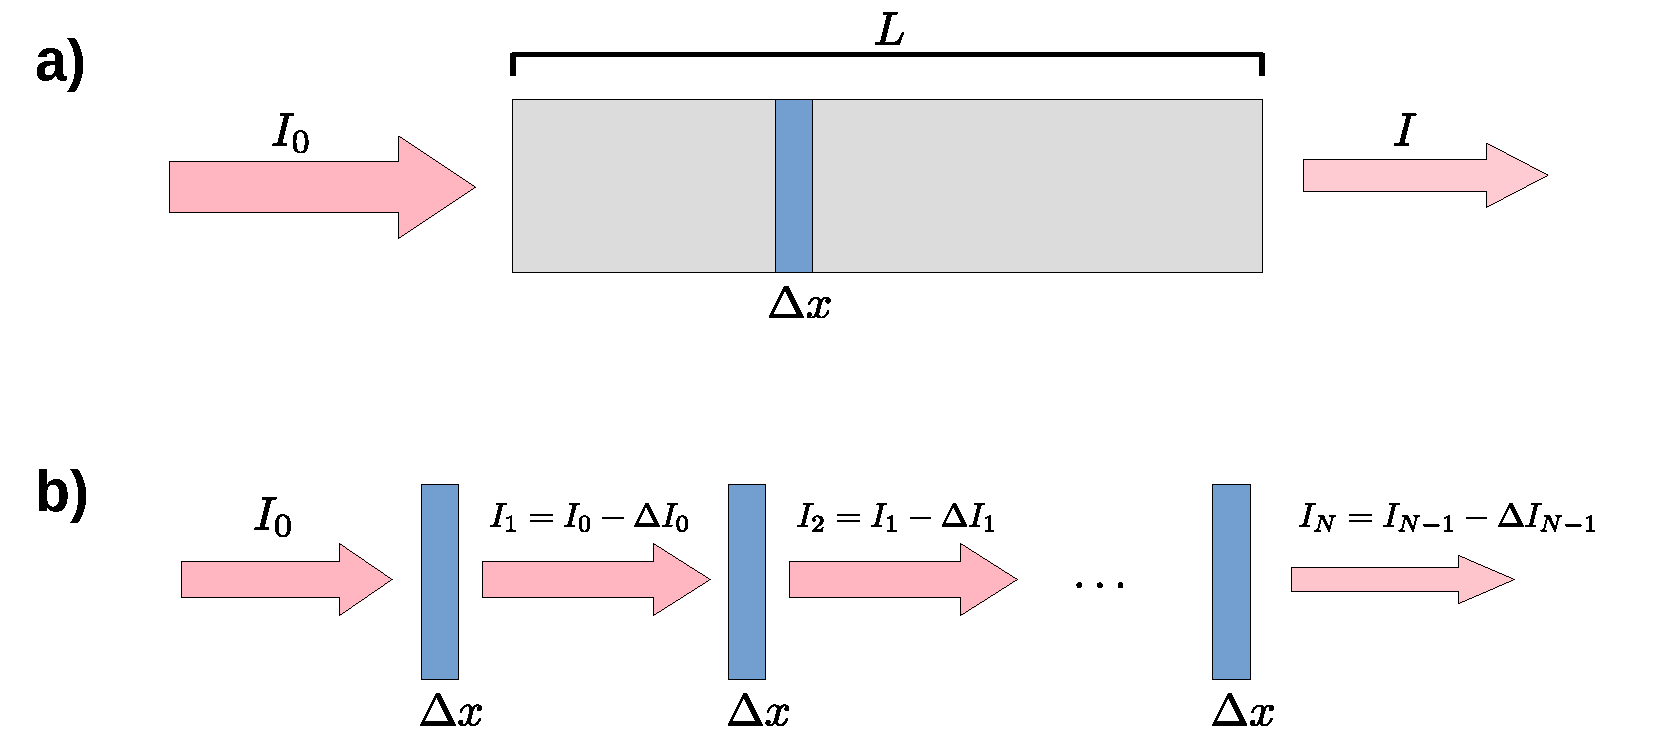
\includegraphics[width=0.7\linewidth]{diagrams/absorption_slabs}
	\caption{The construction of a finite-length absorbing material from many thin slabs. If the material of length $L$ shown in \textbf{a)} is subdivided into slabs of thickness $\Delta x$, then we have a number $N=L/\Delta x$ of such slabs. The Lambert-Beer law is obtained in the limit of the beam traversing infinitely many such absorbing slabs, as shown in \textbf{b)} for $N$ slabs.}
	\label{fig:absorption_slabs}
\end{figure}

After the first slab, the transmitted intensity $I_1$ is
\begin{align}
	I_1 &= I_0 + \Delta I_0 = I_0 \left(1 - \alpha \Delta x\right)
\end{align}
The transmitted intensity after the second slab is $I_2$ given by
\begin{align}
	I_2 &= I_1 + \Delta I_1 = I_1 \left(1 - \alpha \Delta x\right) = I_0 \left(1 - \alpha \Delta x\right)^2
\end{align}
After $N$ slabs, we have traversed the entire medium of thickness $L$. This gives the slice thickness as $\Delta x = L/N$. In terms of the incident intensity $I_0$, this is
\begin{align}
	I_N &= I_0 \left(1 - \alpha \frac{L}{N}\right)^N
\end{align}
In the limit of $N\rightarrow \infty$ slabs, this becomes
\begin{equation}
	I = \lim\limits_{N\rightarrow\infty} I_0 \left(1 - \frac{\alpha L}{N}\right)^N
\end{equation}
Evaluating this limit gives rise to the exponential function, and we arrive at the \textbf{Beer-Lambert law}
\begin{equation} \label{beer-lambert-law}
	I = I_0 e^{-\alpha L}
\end{equation}
This can also be found from (\ref{_beerDiff}) by setting $\Delta I \rightarrow dI$ and $\Delta x \rightarrow dx$ giving a differential equation, and the solution to this differential equation gives the above relation.

Since the value of $\alpha$ at the measurement wavelength is a microscopic property of the absorbing material, measurement of this value yields some information about the material. For a given material that is a solid or liquid, the density of absorbing particles is within a somewhat narrow range and a value of $\alpha$ is sufficient to characterize the optical absorption. For a gas, however, the density of absorbing particles can vary over many orders since the density of the gas varies with temperature and pressure.

In the limiting process depicted in Fig. \ref{fig:absorption_prop}, as the particle cross sectional area is scaled down, the density of particles must be scaled up by the same factor to maintain the same optical extinction. In characterizing the absorption process by opaque scattering objects, the amount of light extinction by each object is characterized by a cross section $\sigma$. If the density of opaque objects is $n$, the limiting process therefore preserves the product $n \sigma = \mathrm{const}$. This leads us to the definition of the optical cross section $\sigma$ through the relation
\begin{equation} \label{alpha_n_sigma}
	\alpha = n \sigma
\end{equation}

\subsection{Absorption Spectrum}
In general the absorption coefficient in (\ref{beer-lambert-law}) is dependent on the wavelength of light that is used for the measurement. A plot of $\alpha(\lambda)$ against the wavelength of light $\lambda$ will be referred to as an absorption spectrum. The absorption spectrum $\alpha(\lambda)$ can be extracted from a measurement of the incident and transmitted spectra, as well as the optical path length through the absorbing material by
\begin{equation}\label{beer_absorp}
	\alpha(\lambda) = -\frac{1}{L}\ln \frac{I(\lambda)}{I_0(\lambda)}
\end{equation}



In this dissertation, we will mostly be concerned with the absorption spectra of gases. For a gas, the absorption coefficient should depend on the density of particles present in the beam path. If we denote the number density as $n$, then the absorption coefficient should be proportional to this density.
\begin{equation}
	\alpha(\lambda) = n \sigma(\lambda)
\end{equation}
The $\sigma$ is referred to as the optical cross section and has units of area.

\subsection{Absorption Coefficient of a Gas Mixture}

\begin{figure}[H]
	\centering
	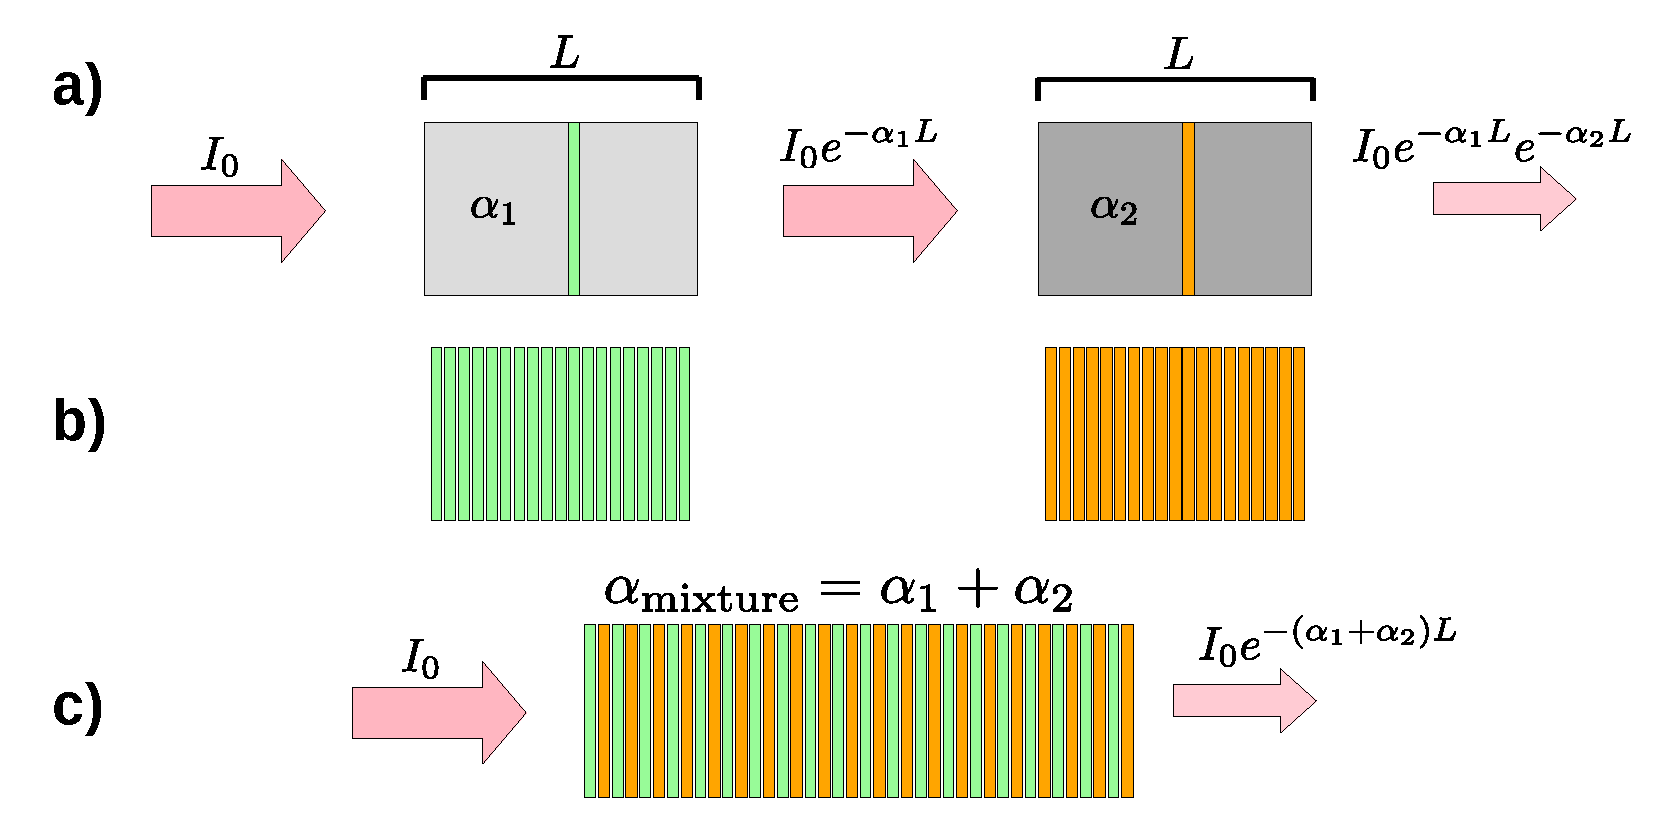
\includegraphics[width=0.7\linewidth]{diagrams/absorption_mixture}
	\caption{Using the thin slab approximation used earlier, a mixture of two gasses is depicted as alternating slabs of the two gas species. As long as the two absorption coefficients $\alpha_1$ and $\alpha_2$ are not affected by the presence of the other gas species, then this gives the same absorption as the beam passing through each pure gas separately.}
	\label{fig:absorptionmixture}
\end{figure}

For a gas mixture having several components, the absorption coefficient is a sum of the absorption coefficients of the individual components
\begin{equation}
	\alpha(\lambda) = \sum_j n_j \sigma_j(\lambda)
\end{equation}
If the mixture behaves as an ideal gas then the total number density is given by the ideal gas law in terms of the total pressure $P$ and temperature $T$
\begin{equation}
	n = \frac{P}{k_b T}
\end{equation}
and the number density of an individual species is given in terms of the partial pressure $p_j$ of that species
\begin{equation}
	n_j = \frac{p_j}{k_b T}
\end{equation}
We define the concentration $c_j$ of an individual species by mole fraction of that species, which for an ideal gas mixture is equivalent to the ratio of the partial pressure of that species to the total pressure. That is $c_j = p_j/P$. We can then write for the absorption coefficient
\begin{align}
	\alpha(\lambda) &= n_1 \sigma_1(\lambda) \;\; + \;\; n_2 \sigma_2(\lambda) \;\; + \;\; \ldots \nonumber \\
	&= \frac{p_1}{k_b T} \sigma_1(\lambda) + \frac{p_1}{k_b T} \sigma_2(\lambda) + \ldots \nonumber \\
	&= \frac{P}{k_b T} \left[\left(\frac{p_1}{P}\right)\sigma_1(\lambda) + \left(\frac{p_1}{P}\right) \sigma_2(\lambda) + \ldots \right] \nonumber\\
	&=\frac{P}{k_b T} \left[c_1\sigma_1(\lambda) + c_2 \sigma_2(\lambda) + \ldots \right]
\end{align}
In terms of the molar concentrations $c_j$, the absorption coefficient is
\begin{equation}\label{alpha_mixture}
	\alpha(\lambda) = \frac{P}{k_b T} \sum_j c_j\sigma_j(\lambda)
\end{equation}
In general the absorption cross section is dependent on the temperature, pressure, and even presence of other gas species. If the cross sections of all species contributing to an absorption signal are known, it then becomes possible to measure the concentrations of the species from an absorption spectrum. This is usually done by fitting an experimentally measured recording of absorption versus wavelength using a model absorption such as (\ref{alpha_mixture}) by finding the concentrations $c_j$ which best reproduce the data.

\section{Linear Least Squares} \label{sec:append_linear_lsq}
Suppose we have $N$ measurements $\{y_1, y_2, \ldots , y_N\}$ taken with parameters $\{x_1, x_2, \ldots , x_N\}$. We then wish to minimize the error to the function
\begin{equation} \label{append_basis_combo}
	f(x) = c_1 f_1(x) + c_2 f_2(x) + \ldots + c_n f_n(x)
\end{equation}
by an appropriate choice of $\{c_1, c_2, \ldots, c_n\}$. That is, we wish to satisfy ``as close as possible'' the equations
\begin{equation}
	y_i = c_1 f_1(x_i) + c_2 f_2(x_i) + \ldots + c_n f_n(x_i)
\end{equation}
for all $N$ sets of measurements. We can write this as an overdetermined $(N>n)$ set of linear equations
\begin{equation} \label{append_lsq_matrix_setup}
	\begin{pmatrix}
		y_1 \\
		y_2 \\
		y_3 \\
		\vdots \\
		y_N
	\end{pmatrix} =
	\begin{pmatrix}
		f_1(x_1) & f_2(x_1) & \ldots & f_n(x_1) \\
		f_1(x_2) & f_2(x_2) & \ldots & f_n(x_2) \\
		f_1(x_3) & f_2(x_3) & \ldots & f_n(x_3) \\
		\vdots & \vdots& \vdots \\
		f_1(x_N) & f_2(x_N) & \ldots & f_n(x_N)
	\end{pmatrix}
	\begin{pmatrix}
		c_1 \\
		c_2 \\
		\vdots \\
		c_n 
	\end{pmatrix}
\end{equation}	
We can write this as
\begin{equation}
	A\vec{c} = \vec{b}
\end{equation}
The least squares solution is acquired by multiplying $A^T$ on both sides to get the \textit{normal equation}
\begin{equation} \label{append_normal_equation}
	A^T A \vec{c} = A^T \vec{b}
\end{equation}
This system can then be solved by inverting the square $A^T A$ matrix and left multiply the normal equation by this inverse to obtain the least squares solution
\begin{equation}\label{append_leastSquares}
	\boxed{\vec{c} = (A^T A)^{-1} A^T \vec{b}}
\end{equation}

\subsection{The Normal Equation -- Connection to Error Minimization}

We will show that the least squares solution (\ref{append_leastSquares}) minimizes the sum of the squared errors given by
\begin{equation}
	E = \sum_i \Big[ y_i - f(x_i) \Big]^2 = (A\vec{c} - \vec{b})^T (A\vec{c} - \vec{b})
\end{equation}
This is equivalent to minimizing by our choice in $c_1\ldots c_n$ the scalar quantity
\begin{equation} \label{append_error}
	E = \sum_i \Big[ y_i - \left( c_1 f_1(x_i) + c_2 f_2(x_i) + \ldots + c_n f_n(x_i) \right) \Big]^2
\end{equation}
We can see this by setting the derivative of $E$ with respect to each $c_{1\ldots n}$ coefficient equal to zero. We write this in the vector notation
\begin{equation}
	\frac{\partial E}{\partial \vec{c}} = \vec{0}
\end{equation}
Substituting the above definition of $E$, this is
\begin{align}
	\vec{0} = \frac{\partial E}{\partial \vec{c}} &= \frac{\partial}{\partial \vec{c}} \left[(A\vec{c} - \vec{b})^T (A\vec{c} - \vec{b})\right]
\end{align}
We write this $n$ component equation in index notation following the Einstein summation convention, where repeated indices imply summation. We write the $i^\mathrm{th}$ component of the column vector $\vec{c}$ and its transpose as $\left(\vec{c}\,\right)_i=c_i$ and $\left(c^T\right)_i = c_{0i}$. The $i^\mathrm{th}$ component of the above equation is then
\begin{align}
	%0 &= \frac{\partial E}{\partial c_{i}} \left[(A\vec{c} - \vec{b})^T_{j} (A\vec{c} - \vec{b})_{j}\right] \nonumber\\
	0 &= \frac{\partial E}{\partial c_{i}} \left[(c^T A^T - b^T)_{j} (A\vec{c} - \vec{b})_{j}\right] \nonumber\\
	&= \frac{\partial E}{\partial c_{i}} \Big[(c_{0k}A_{jk} - b_{0j}) (A_{jl}c_{l} - b_j)\Big] \nonumber\\
	&= \frac{\partial E}{\partial c_{i}} \Big[ c_{0k}A_{jk}A_{jl}c_l - c_{0k}A_{jk}b_j - b_{0j}A_{jl}c_l + b_{0j}b_j \Big] \nonumber\\
	&= \delta_{ik}A_{jk}A_{jl}c_l + c_{0k}A_{jk}A_{jl}\delta_{li} - \delta_{ik}A_{jk}b_j - b_{0j}A_{jl}\delta_{li} \nonumber\\
	&= A_{ji}A_{jk}c_k + c_{0k}A_{jk}A_{ji} - A_{ji}b_j - b_{0j}A_{ji}
\end{align}
In the last step we have substituted the dummy index $l\rightarrow k$. We can see that have the same operations written twice since $c_{0k} = c_k$ and $b_{0j}=b_j$. Coming back to vector-matrix notation, the above expression is the same as
\begin{align}
	\vec{0} = 2\left(A^T A \vec{c} - A^T \vec{b}\right)
\end{align}
This then leads us again to the normal equation
\begin{equation}
	A^T A \vec{c} = A^T \vec{b}
\end{equation}

\subsubsection{Checking the Minimum}
We can check that the solution to the normal equation above provides a true minimum of the error $E$ by computing the second derivative with respect to each coefficient $c_i$. To avoid confusion in the Einstein convention with repeated $i$ index, we write the sums explicitly
\begin{align}
	\frac{\partial^2 E}{\partial c_i^2}
	&= \frac{\partial}{\partial c_i} \Big[\sum_{j,k}A_{ji}A_{jk}c_k + \sum_{j,k}c_{0k}A_{jk}A_{ji} - \sum_{j}A_{ji}b_j - \sum_{j}b_{0j}A_{ji}\Big] \nonumber\\
	&= \sum_{j,k}A_{ji}A_{jk}\delta_{ki} + \sum_{j,k}\delta_{ik}A_{jk}A_{ji} \nonumber\\
	&= 2\sum_{j}\left(A_{ji}\right)^2 \nonumber\\
	\frac{\partial^2 E}{\partial c_i^2} &> 0
\end{align}
Since the above second derivative is positive for every $i$, we see that the solution given by the normal equation is indeed a true minimum. We therefore conclude that the least-squares solution (\ref{append_leastSquares}) gives the set of coefficient $c_i$ which minimize the error sum in (\ref{append_error}).

\subsection{Two Component Solution}
We assume that we have two function $f_{1,2}(x)$ which are to be fit to the data using the model function
\begin{equation}
	f(x) = c_1 f_1(x) + c_2 f_2(x)
\end{equation}
The $N\times 2$ matrix $A$ is then
\begin{equation}
	A =
	\begin{pmatrix}
		f_1(\vec{x}) & f_2(\vec{x})
	\end{pmatrix}
\end{equation}
We proceed to compute
\begin{equation}
	A^T A =
	%\begin{pmatrix}
	%	f_1(\vec{x})\cdot f_1(\vec{x}) & f_2(\vec{x})\cdot f_1(\vec{x}) \\
	%		f_1(\vec{x})\cdot f_2(\vec{x}) & f_2(\vec{x})\cdot f_2(\vec{x})
	%\end{pmatrix}
	%=
	\begin{pmatrix}
		\sum_i f_1(x_i)^2 & \sum_i f_1(x_i)f_2(x_i) \\
		\sum_i f_2(x_i)f_1(x_i) & \sum_i f_2(x_i)^2
	\end{pmatrix}
	\equiv
	\begin{pmatrix}
		a_{11} & a_{12} \\
		a_{12} & a_{22}
	\end{pmatrix}
\end{equation}
We can immediately invert the 2x2 matrix to give
\begin{equation}
	\left(A^T A\right)^{-1} = 
	%\frac{1}{\left(\sum_i f_1(x_i)^2\right)\left(\sum_i f_2(x_i)^2\right) - \left(\sum_i f_1(x_i)f_2(x_i)\right)^2}
	\frac{1}{a_{11} a_{22} - a_{12}^2}
	\begin{pmatrix}
		a_{22} & -a_{12} \\
		-a_{12} & a_{11}
	\end{pmatrix}
\end{equation}
We now construct the matrix
\begin{equation}
	\left(A^T A\right)^{-1} A^T = \frac{1}{a_{11} a_{22} - a_{12}^2}
	\begin{pmatrix}
		a_{22}f_1(x^T)  - a_{12}f_2(x^T) \\
		-a_{12}f_1(x^T) + a_{11}f_2(x^T)
	\end{pmatrix}
\end{equation}
The coefficients $c_{1,2}$ are then given by the two components of $\left(A^T A\right)^{-1} A^T \vec{b}$. If we define $\tilde{a}_1 \equiv \sum_i y_i f_1(x_i)$ and $\tilde{a}_2 \equiv \sum_i y_i f_2(x_i)$ then we have the following formulas for the values of the fit coefficients
\begin{align} \label{append_lsq_two_comp}
	c_1 = \frac{a_{22}\tilde{a}_1 - a_{12} \tilde{a}_2}{a_{11} a_{22} - a_{12}^2}
	&\qquad&
	c_2 = \frac{a_{11}\tilde{a}_2 - a_{12} \tilde{a}_1}{a_{11} a_{22} - a_{12}^2}
\end{align}

\subsubsection{Linear Regression Formula}
Fitting a line to a set of experimentally recorded data is a task that is often used. For this we use the two component equation with
\begin{equation}
	f(x_i) = c_1 x_i + c_0
\end{equation}
This gives for the five $a$ coefficients
\begin{align}
	a_{11} = \sum_i x_i^2 && a_{12} = \sum_i x_i && a_{22}=N && \tilde{a}_1 = \sum_i y_i x_i && \tilde{a}_2 = \sum_i y_i
\end{align}
This gives the regression formula for the slope
\begin{equation}\label{append_linreg_slope}
	c_1 = \frac{N\sum x_i y_i - \left(\sum x_i\right)\left(\sum y_i\right)}{N\sum x_i^2 - \left(\sum x_i\right)^2}
\end{equation}
and for the intercept
\begin{equation}\label{append_linreg_interc}
	c_0 = \frac{\left(\sum x_i^2\right)\left(\sum y_i\right) - \left(\sum x_i\right)\left(\sum x_i y_i\right)}{N\sum x_i^2 - \left(\sum x_i\right)^2} = \bar{y_i} - c_1 \bar{x_i}
\end{equation}




\subsection{Uncertainty in the Coefficients}

For a general nonlinear function $g(x_1, x_2, \ldots, x_n)$ of the $n$ parameters $x_i$, we can estimate the deviation $\Delta g$ of the function output given the statistically independent deviations $\Delta x_1$, $\Delta {x_2}$, $\ldots$, $\Delta {x_n}$ of the input parameters by the law of propagation of errors \cite{stats_lawOfPropagationErrs}
\begin{equation} \label{append_error_prop}
	\Delta g^2 =
	\left(\frac{\partial g}{\partial x_1}\Bigg|_{\tilde{x}_1}\right)^2 \Delta {x_1}^2 +
	\left(\frac{\partial g}{\partial x_2}\Bigg|_{\tilde{x}_2}\right)^2 \Delta {x_2}^2 + \ldots +
	\left(\frac{\partial g}{\partial x_n}\Bigg|_{\tilde{x}_n}\right)^2 \Delta {x_n}^2
\end{equation}
The $\tilde{x}_i$ in the above expression are the average values of each of the $x_i$.

We consider the case of (\ref{append_leastSquares}), where for simplicity we denonte the pseudoinverse matrix $M = \left(A^T A\right)^{-1} A^T$. The function under consideration is then linear in the measured ordinate values $\vec{b}$
\begin{equation} \label{append_error_ci}
	c_i = \sum_{j} M_{ij}b_j
\end{equation}
From the law of propagation of errors (\ref{append_error_prop}), we have that the deviation of the concentration of the $i^\mathrm{th}$ coefficient is
\begin{equation}
	\Delta {c_i}^2 = \sum_{k} \left(\frac{\partial c_i}{\partial b_k}\Bigg|_{\tilde{b}_k}\right)^2 \Delta {b_k}^2
\end{equation}
From (\ref{append_error_ci}) we can evaluate the partial derivative in the above expression. There is no dependence of the matrix $M$ on the measured ordinate values $\partial M / \partial b_k = 0$, since $M$ is calculated from the functional dependences of the $f_{1\ldots n}(x)$ basis set used. With the trivial action of the partial derivative on the linear terms $\partial b_j / \partial b_k = \delta_{jk}$ we have
\begin{equation}
	\frac{\partial c_i}{\partial b_k}\Bigg|_{\tilde{b}_k} = \sum_j M_{ij} \delta_{jk} = M_{ik}
\end{equation}
We then have the deviation of the $i^\mathrm{th}$ coefficient as
%\label{error_conc_alpha} !!!!!
\begin{equation} \label{append_leastSq_error}
	\boxed{\Delta {c_i} = \sqrt{\sum_j \left(M_{ij} \, \Delta {b_j}\right)^2}}
\end{equation}

%That is, the fluctuation in the concentration is calculated in terms of the fluctuation in the measured absorption. It is now clear that measurements of the absorption coefficient which are homoscedastic, where the uncertainties of all measurements is a constant $\Delta x_i = \Delta x$, then the precision of the concentration determination scales linearly with the precision of absorption coefficient determination $\Delta c_i \propto \Delta x$.

\subsubsection{Single Basis Function Scale Uncertainty}
We consider here the specialized case of just a single basis function
$$f(x) = c_1 f_1(x)$$
The matrix then $A$ becomes that of a single column vector $\vec{f_1}$ defined as $\left(\vec{f}_1\right)_i \equiv f_1(x_i)$. It is clear in this case that $A^T A$ is just a scalar, and the matrix $M = \left(A^T A\right)^{-1} A^T$ is then just the row vector
\begin{equation}
	M = \frac{A^T}{\vec{A}\cdot \vec{A}} = \frac{f_1^T}{\vec{f_1}\cdot\vec{f_1}}
\end{equation}
Using that $M=M_{0j}$, we have from (\ref{append_leastSq_error}) the basis function scale uncertainty
\begin{equation}\label{append_error_one_general}
	\Delta c = \frac{1}{\vec{f}_1\cdot\vec{f}_1} \sqrt{\sum_j \Big(f_1(\lambda_j) \, \Delta b_j\Big)^2}
\end{equation}

For measurements that are homoscedastic, or have constant uncertainty, $\Delta b_i \equiv \Delta b$, this relation simplifies to
\begin{equation}
	\boxed{\Delta c = \frac{\Delta b}{\left|\vec{f}_1\right|}}
\end{equation}
If all of the $N$ measurements are conducted at a single input value $x_i = \tilde{x}$ where the basis function has the value $f_1 = f(\tilde{x})$, then this gives the same effect as averaging those measurements
\begin{equation}
	\boxed{\Delta c_\mathrm{avg} = \frac{\Delta b}{\sqrt{N} f_1}}
\end{equation}
For measurements all corresponding to the same $x$ value, we see that \textit{there is no difference between averaging the measured values or entering them each as separate measurements into (\ref{append_lsq_matrix_setup})}.	


\subsubsection{Coefficient Uncertainty for Two Basis Functions}
For a function given by the linear combination of two basis functions \newline $f(x) = c_1 f_1(x) + c_2 f_2(x)$, then we have the generally overdetermined $(N>2)$ system
\begin{equation*}
	\underbrace{\begin{pmatrix}
			b_1 \\
			b_2 \\
			b_3 \\
			\vdots \\
			b_N
	\end{pmatrix}}_{\begin{matrix}\vec{b}\end{matrix}} =
	\underbrace{\begin{pmatrix}
			f_1(x_1) &  f_2(x_1) \\
			f_1(x_2) &  f_2(x_2) \\
			f_1(x_3) &  f_2(x_3) \\
			\vdots & \vdots \\
			f_1(\lambda_N) & f_2(x_N)
	\end{pmatrix}}_{\begin{matrix}A\end{matrix}}
	\begin{pmatrix}
		b_1 \\
		b_2
	\end{pmatrix}
\end{equation*}
We define the corresponding vectors $\vec{f}_1$ and $\vec{f}_2$ having entries $\left(\vec{f}_{1,2}\right)_i = f_{1,2}(x_i)$ corresponding to the evaluations of each function at the measurement values $x_i$. We then have the matrices
\begin{align}
	A =
	\begin{pmatrix}
		\vec{f}_1 & \vec{f}_2
	\end{pmatrix}
	&&
	A^T =
	\begin{pmatrix}
		f_1^T \\ f_2^T
	\end{pmatrix}
	&&
	A^T A =
	\begin{pmatrix}
		\vec{f}_1 \cdot \vec{f}_1 & \vec{f}_1 \cdot \vec{f}_2 \\
		\vec{f}_2 \cdot \vec{f}_1 & \vec{f}_2 \cdot \vec{f}_2
	\end{pmatrix}
\end{align}
We see that the matrix $A^T A$ is of dimension 2x2 having entries corresponding to the scalar products of the $\vec{f}_{1,2}$ vectors. For a general 2x2 matrix having nonzero determinant, we have the inverse
\begin{equation*}
	\begin{pmatrix}
		a & b \\ c & d
	\end{pmatrix} ^ {-1}
	=
	\frac{1}{ad - bc}
	\begin{pmatrix}
		d & -b \\ -c & a
	\end{pmatrix}
\end{equation*}
In constructing the $M$ matrix, we require the inverse
\begin{equation}
	\left(A^T A\right)^{-1} = \frac{1}{f_1^2 f_2^2 - \left(\vec{f}_1\cdot\vec{f}_2\right)^2}
	\begin{pmatrix}
		f_2^2 & -\vec{f}_1\cdot\vec{f}_2 \\
		-\vec{f}_1\cdot\vec{f}_2 & f_1^2
	\end{pmatrix}
\end{equation}
Right-multiplying the above expression by $A^T$ gives the $M$ matrix
%	\begin{equation}
	%		M = \frac{k_\mathrm{B} T / P}{f_1^2 f_2^2 - \left(\vec{f}_1\cdot\vec{f}_2\right)^2}
	%		\begin{pmatrix}
		%			\;\;\;
		%			f_2^2 f_1^T - \left(\vec{f}_1 \cdot \vec{f}_2\right)f_2^T \\\\
		%			-\left(\vec{f}_1 \cdot \vec{f}_2\right)f_1^T + f_1^2 f_2^T
		%		\end{pmatrix}
	%	\end{equation}
\begin{equation}
	M = \frac{1}{f_1^2 f_2^2 - \left(\vec{f}_1\cdot\vec{f}_2\right)^2}
	\left[
	\begin{pmatrix} f_2^2 \\ -\vec{f}_1 \cdot \vec{f}_2 \end{pmatrix} f_1^T +
	\begin{pmatrix} -\vec{f}_1 \cdot \vec{f}_2 \\ f_1^2 \end{pmatrix} f_2^T
	\right]
\end{equation}
We define the overlap parameter $\gamma$ which measures the cosine of the angle between the \newline $\vec{f}_1$ and $\vec{f}_2$ vectors
\begin{equation}
	\gamma \equiv \frac{\vec f_1\cdot\vec f_2}{f_1f_2}
\end{equation}
This parameter ranges from $\pm 1$, where a value of $\left|\gamma\right| = 1$ means that $f_1$ and $f_2$ are identical up to a scale factor. In terms of the overlap parameter, the $M$ matrix is
\begin{equation}
	M = \frac{1}{1 - \gamma^2}
	\left[
	\begin{pmatrix} 1/f_1^2 \\ -\gamma/f_1f_2 \end{pmatrix} f_1^T +
	\begin{pmatrix} -\gamma/f_1f_2 \\ 1/f_2^2 \end{pmatrix} f_2^T
	\right]
\end{equation}
From (\ref{append_leastSq_error}) the errors in the coefficient estimates are
%	\begin{equation} \label{error_two_general}
	%		\begin{pmatrix}
		%			\Delta c_1 \\ \Delta c_2
		%		\end{pmatrix} = 
	%		\frac{k_\mathrm{B} T / P}{f_1^2 f_2^2 - \left(\vec{f}_1 \cdot \vec{f}_2\right)^2}
	%		\begin{pmatrix}
		%			\sqrt{\sum_i \Delta x_i\Big( f_2^2 f_{1,i} - (\vec f_1\cdot\vec f_2)f_{2,i} \Big)^2} \\ \\
		%			\sqrt{\sum_i \Delta x_i\Big( f_1^2 f_{2,i} - (\vec f_1\cdot\vec f_2)f_{1,i} \Big)^2}
		%		\end{pmatrix}
	%	\end{equation}
\begin{equation} \label{append_error_two_general}
	\begin{pmatrix}
		\Delta c_1 \\ \Delta c_2
	\end{pmatrix} = 
	\frac{1}{1 - \gamma^2}
	\begin{pmatrix}
		\sqrt{\sum_i \Delta b_i\left( \frac{1}{f_1^2}f_{1,i} - \frac{\gamma}{f_1f_2}f_{2,i} \right)^2} \\ \\
		\sqrt{\sum_i \Delta b_i\left( \frac{1}{f_2^2}f_{2,i} - \frac{\gamma}{f_1f_2}f_{1,i} \right)^2}
	\end{pmatrix}
\end{equation}
For $\gamma = 0$, corresponding to completely orthogonal $\vec{f}_1$ and $\vec{f}_2$, this gives the equivalent of (\ref{append_error_one_general}) for two independent detections when there is zero overlap between the basis functions
\begin{equation}
	\Delta c_{i} \approxeq \frac{1}{f_{i}^2} \sqrt{\sum_j \left(f_{i,j}\, \Delta b_j\right)}
\end{equation}

For measurements having constant uncertainty $\Delta  b_i = \Delta  b$, we can expand each term in the sums in equation (\ref{append_error_two_general}). For the first row, we have
\begin{equation}
	\sum_i\left(\frac{1}{f_1^2}f_{1,i} - \frac{\gamma}{f_1f_2}f_{2,i}\right)^2 = \sum_i\left(\frac{f_{1,i}^2}{f_1^4} + \frac{\gamma^2f_{2,i}^2}{f_1^2f_2^2} - 2\frac{\gamma}{f_1^3f_2}f_{1,i}f_{2,i}\right) = \frac{1}{f_1^2} - \frac{\gamma^2}{f_1^2}
\end{equation}
The second row is given simply by interchanging the $1$ and $2$ subscripts in the basis functions. In the last step we have used that $\sum_i f_{1,i}^2 = f_1^2$ and $\sum_i f_{1,i}f_{2,i} = f_1f_2\gamma$. For the case of constant measurement uncertainty, equation (\ref{append_error_two_general}) then simplifies to
\begin{equation}\label{append_error_two_constUnc}
	\boxed{\Delta c_i = 
		\frac{\Delta  b}{\left|\vec f_i\right| }
		\frac{1}{\sqrt{1 - \gamma^2}}}
\end{equation}

\subsubsection{Unresolved Baseline}
Using as $f_2(\lambda) = 1$, the corresponding vector, magnitude and overlap parameter are
\begin{eqnarray}
	\vec{f}_2 = \vec{1} &\qquad
	f_2 ^2 = N &\qquad
	\gamma = \frac{\vec{f}_1 \cdot \vec{f}_2}{\left|\vec f_1\right|\sqrt{N}} = \frac{1}{\sqrt{N}\left|\vec f_1\right|}\sum_i f_{1,i} \equiv \frac{f_\mathrm{Avg}}{f_\mathrm{RMS}}
\end{eqnarray}
Above we have defined the average function value $f_\mathrm{Avg} \equiv \frac{1}{N}\sum_i f_{1,i}$ and the root-mean-square value $f_\mathrm{RMS} \equiv \sqrt{\frac{1}{N}\sum_i f_{1,i}^2} = \left|\vec f_1\right|/\sqrt{N}$.
The uncertainty of the coefficients are then
\begin{align}
	\Delta c &= \frac{\Delta b}{\sqrt{N}}\frac{1}{\sqrt{f_\mathrm{RMS}^2 - f_\mathrm{Avg}^2}} \\\nonumber\\
	\Delta B &= \frac{\Delta b}{\sqrt{N}}\frac{1}{\sqrt{1 - f_\mathrm{Avg}^2/f_\mathrm{RMS}^2}}
\end{align}

\subsubsection{General Basis}
\begin{align}
	A = 
	\begin{pmatrix}
		\vec{f}_1 & \vec{f}_2 & \ldots & \vec f_m
	\end{pmatrix}
	&&
	A^T =
	\begin{pmatrix}
		f_1^T \\ f_2^T \\ \vdots \\ f_m^T
	\end{pmatrix}
	&&
	A^T A = 
	\begin{pmatrix}
		\vec{f}_1 \cdot \vec{f}_1 & \vec{f}_1 \cdot \vec{f}_2 & \ldots & \vec f_1\cdot\vec f_m \\
		\vec{f}_2 \cdot \vec{f}_1 & \vec{f}_2 \cdot \vec{f}_2 & \ldots & \vec{f}_2 \cdot \vec{f}_m \\
		\vdots & \vdots\ & \ddots & \vdots \\
		\vec{f}_m \cdot \vec{f}_1 & \vec{f}_m \cdot \vec{f}_2 & \ldots & \vec f_m\cdot\vec f_m
	\end{pmatrix}
\end{align}
The element in the $i^\mathrm{th}$ row and $j^\mathrm{th}$ column of the $A^TA$ matrix is
\begin{equation}
	B_{ij} \equiv \left(A^TA\right)_{ij} = \vec f_i\cdot\vec f_j
\end{equation}
The inverse of this matrix is written in terms of the minors $M_{ij}$
\begin{equation}
	\left(B^{-1}\right)_{ij} = \frac{(-1)^{i+j}M_{ij}}{\det\left(B\right)}
\end{equation}
Using the Levi-Civita symbols, we write this as
\begin{equation}
	\left(B^{-1}\right)_{ij} = \frac{1}{(n-1)!\det\left(B\right)}\epsilon_{i i_2\ldots i_n}\epsilon_{j j_2\ldots j_n}B_{i_2j_2}B_{i_3j_3}\ldots B_{i_nj_n}
\end{equation}

\section{Series Derivation of CRDS Weight Function} \label{sec:append_weight_series_crds}

%For this discussion we will drop the dependence on wavelength of the baseline ring-down time $\tau_0(\lambda) \rightarrow \tau_0$ and assume it is constant. 

Under the non-interacting gas approximation discussed in Sec. \ref{chap:fitting_spectra}, the model absorption of a gas mixture is simply a linear combination of known absorption cross section functions
\begin{equation}
	\alpha_\mathrm{m}(\lambda) = a_1 \sigma_1 (\lambda) + \ldots + a_n \sigma_n(\lambda)
\end{equation}
having unknown proportional coefficients. These proportional coefficients are determined by setting up the over-determined system given by (\ref{fit_spectrum})
and then the least-squares solution to the above system is given at once by (\ref{leastSquares}), or equivalently (\ref{append_leastSquares}). In the case of Cavity Ringdown Spectroscopy (CRDS), the absorption coefficient is determined by a nonlinear transformation of the ringdown time
\begin{equation}\label{alpha_crds_appdx}
	c\alpha_i \equiv c\alpha(\tau_i) = \tau_i^{-1} - \tau_0^{-1}
\end{equation}
The set of coefficients $a_j$ given by this solution are such that the quantity
\begin{align} \label{error_alpha}
	\mathrm{E}_\alpha &= \sum_{i} \left[ \alpha_i - \alpha_\text{m}(\lambda_i) \right]^2 \nonumber \\
	&= \sum_{i} \left[\frac{1}{c}\left(\frac{1}{\tau_i} - \frac{1}{\tau_0} \right) - \alpha_\mathrm{m}(\lambda_i) \right]^2
\end{align}
is minimized. A potential problem with this scheme is that the deviation in the absorption measurements $\Delta \alpha$ is not homoscedastic and the deviation changes over the potential range of absorption magnitudes. 

For a ring-down time measurement dominated by technical noise rather than systematic effects, the relative deviation of these measurements $\Delta\tau/\bar{\tau}$ is approximately constant \cite{vanZee_1999}, where $\bar\tau$ is the mean of the measurements. This behavior is confirmed in our experiment as indicated by the histograms in Fig. \ref{fig:crds_detectionlimit}. If we transform the measurements by a function $f(\tau)$ then the deviation of the resulting function values are $\Delta f = \left|f'(\bar\tau)\right| \Delta \tau$. Choosing $f(\tau) = \ln(\tau/\tau_0)$ gives a variance $\Delta f = \Delta \tau/\bar{\tau}$ which is approximately constant. This implies that we should minimize the error in log-space
\begin{align} \label{error_log}
	\mathrm{E}_\mathrm{L} &= \sum_i \Big[\ln \frac{\tau_i}{\tau_0} - \ln\frac{\tau_\mathrm{model}(\lambda_i)}{\tau_0}\Big]^2 \nonumber \\
	&= \sum_i \Big[\ln \frac{\tau_i}{\tau_0} + \ln\big(1+c\tau_0\alpha_\mathrm{m}(\lambda_i)\big)\Big]^2
\end{align}
Where we have the simulated ring-down time from the inverse of equation (\ref{alpha_crds_appdx}) applied to the model absorption
\begin{equation}
	\tau_\mathrm{model}(\lambda) = \frac{1}{c\alpha_\mathrm{m}(\lambda) + 1/\tau_0}
\end{equation}
Unlike $E_\alpha$, the unknown $a_i$ coefficients do not appear linearly in the transformed error $E_\mathrm{L}$, and the solutions for $a_i$ which minimize this sum cannot be written as a simple equation. We instead proceed by choosing a weight function which transforms the solution for $E_\alpha$ into one which approximates that of $E_\mathrm{L}$.

The set of $N$ equations given by (\ref{fit_spectrum}) can each be multiplied by a constant factor without affecting the equality of each equation. If we choose this factor to depend on the value of the ring-down time measurement $w(\tau_i)$, then the least-squares solution (\ref{append_leastSquares}) is affected by shifting the relative importance of each equation in the sum. The least-squares solution which is obtained from the weighted set of equations is that which minimizes the sum
\begin{align}
	\mathrm{E}_{\alpha,w} &= \sum_{i}  \Big[\alpha(\tau_i)w(\tau_i) - \alpha_\text{m}(\lambda_i)w(\tau_i) \Big]^2
\end{align}
We analyze this sum by Taylor expanding the terms separately for small absorption. Specifically, we expand the left term about the corresponding point of ring-down time nearly equal to the baseline $\tau \sim \tau_0$, and the right term about the point of zero absorption $c\tau_0\alpha_m \sim 0$.
\begin{align} \label{expan_alphaW}
	\mathrm{E}_{\alpha,w} \simeq&
	\left(\frac{1}{c\tau_0}\right)^2 \sum_{i} \Bigg[
	A_1\left(\frac{\tau_i-\tau_0}{\tau_0}\right) + A_2\left(\frac{\tau_i-\tau_0}{\tau_0}\right)^2 + \ldots \nonumber \\
	&+ w(\tau_0)c\tau_0\alpha_\mathrm{m}(\lambda_i) + c\tau_0\alpha_\mathrm{m}(\lambda_i) \Big[w(\tau_i) - w(\tau_0)\Big]
	\Bigg]^2
\end{align}
Where the
\begin{equation}
	A_n = (-1)^{n-1}\sum_{k=0}^{n-1}\frac{(-\tau_0)^k}{k!}w^{(k)}(\tau_0)
\end{equation}
result from the Taylor expansion of $\alpha(\tau_i)w(\tau_i)$ about the point $\tau_0$, and the use of the generalized Leibniz rule to evaluate the derivative terms. We give the first few values of the number $A_n$ which are expressed as derivatives of the weight function evaluated at the baseline ring-down time
\begin{align}
	A_1 &= w(\tau_0) \\
	A_2 &= \tau_0w'(\tau_0) - w(\tau_0) \\
	A_3 &= \frac{1}{2}\tau_0^2w''(\tau_0) - \tau_0w'(\tau_0) + w(\tau_0)
\end{align}
It can be seen that the $A_n$ obey the recursion relation
\begin{equation} \label{A_recurs}
	A_{n+1} =  \frac{(\tau_0)^n}{n!}w^{(n)}(\tau_0) - A_n
\end{equation}

We perform an expansion of the log-space error $E_\mathrm{L}$ given by (\ref{error_log}) in small absorption about the point $\tau \sim \tau_0$
\begin{align} \label{expan_log}
	\mathrm{E}_\mathrm{L} &\simeq
	\sum_i \Bigg[
	\frac{\tau_i - \tau_0}{\tau_0} - \frac{\left(\tau_i-\tau_0\right)^2}{2\tau_0^2} +
	\frac{\left(\tau_i - \tau_0\right)^3}{3\tau_0^4} - \ldots \nonumber \\
	&+ c\tau_0\alpha_\mathrm{m}(\lambda_i) %\nonumber \\
	+ c\tau_0 \alpha_\mathrm{m}(\lambda_i)\left(-\frac{1}{2}c\tau_0\alpha_m(\lambda_i) + \frac{1}{3}c^2\tau_0^2\alpha^2_\mathrm{m}(\lambda_i) - \ldots\right)
	\Bigg]^2
\end{align}
It can be seen that first order agreement between (\ref{expan_alphaW}) and (\ref{expan_log}) is obtained when we set $w(\tau_0) = 1$. Second order agreement of the two expansions in $(\tau_i-\tau_0)/\tau_0$ is obtained when we set $A_2=-1/2$ which gives $w'(\tau_0) = 1/2\tau_0$.

To compare the terms in the parentheses of (\ref{expan_log}) to equivalent terms in the weighted sum (\ref{expan_alphaW}), we must linearize these terms in the absorption model $\alpha_m$. We replace the higher order terms of $\alpha_m$ with the measured absorption $\alpha_i$ using the rule $c\tau_0\alpha_m(\lambda_i)\rightarrow \left(\frac{\tau_0}{\tau_i}-1\right)$. This gives the auxiliary condition for agreement between (\ref{expan_alphaW}) and (\ref{expan_log})
\begin{equation} \label{check_1st_order_log}
	w(\tau_i) - w(\tau_0) \simeq -\frac{1}{2}\left(\frac{\tau_0}{\tau_i}-1\right) \simeq \frac{\tau_i-\tau_0}{2\tau_0}
\end{equation}
The condition above, along with $w(\tau_0)=1$ and $w'(\tau_0)=1/2\tau_0$ is satisfied by $w_\mathrm{L}(\tau) \simeq 1 + \frac{\tau-\tau_0}{2\tau_0}$. Note that this linear function is already determined by the conditions on $w(\tau_0)$ and $w'(\tau_0)$, but happens to also fulfill the auxiliary condition.

We can continue this process to higher order indefinitely by setting $A_n=(-1)^{n+1}/n$ to match each terms appearing from the expansion of $\ln\left(\tau_i/\tau_0\right)$. From (\ref{A_recurs}) we can then solve for the n$^\mathrm{th}$ derivative of the weight function
\begin{equation}
	w^{(n)}(\tau_0) = \frac{n!(-1)^{n-1}}{\tau_0^n}\left(\frac{1}{n}-\frac{1}{n+1}\right)
\end{equation}
allowing us to construct the full Taylor series for the weight function
\begin{equation}
	w_\mathrm{L}(\tau) = 1+\sum_{n=1}^{\infty}(-1)^{n-1}\left(\frac{1}{n}-\frac{1}{n+1}\right)\left(\frac{\tau-\tau_0}{\tau_0}\right)^n
\end{equation}
The resulting telescoping series can then be evaluated in closed form as
\begin{equation} \label{weight_log}
	%w_\mathrm{L}(\tau) = \frac{\frac{\tau}{\tau_0}\ln\frac{\tau}{\tau_0}}{\frac{\tau}{\tau_0}-1}
	w_\mathrm{L}(\tau) = \frac{\tau\ln\frac{\tau}{\tau_0}}{\tau-\tau_0}
\end{equation}
The weight function $w_\mathrm{L}(\tau)$ we have constructed also satisfies the same auxiliary condition demanded earlier to all orders
\begin{equation}
	w_\mathrm{L}(\tau_i) - w_\mathrm{L}(\tau_0) = -\frac{1}{2}\left(\frac{\tau_0}{\tau_i}-1\right) + \frac{1}{3}\left(\frac{\tau_0}{\tau_i}-1\right)^2 - \frac{1}{4}\left(\frac{\tau_0}{\tau_i}-1\right)^3 + \ldots
\end{equation}
which is obtained using the replacement rule $c\tau_0\alpha_m(\lambda_i)\rightarrow \left(\frac{\tau_0}{\tau_i}-1\right)$ in the parenthetical terms of Eq. (\ref{expan_log}) and comparing to (\ref{expan_alphaW}).

The expansion of $\ln(1+c\tau_0\alpha_\mathrm{m})$ used to go from (\ref{error_log}) to (\ref{expan_log}) is only valid for $c\tau_0\alpha_\mathrm{m} \leq 1$. This can be improved if instead we expand about the point $c\tau_0\alpha_\mathrm{m} = 1$, giving an improved radius of convergence up to a larger absorption of $c\tau_0\alpha_\mathrm{m} \leq 3$. We must correspondingly expand $\ln(\tau/\tau_0)$ about the point $\tau = \tau_0/2$. The radius of convergence of this expansion still captures the entire dynamic range $0 < \tau < \tau_0$. The result of performing the above process about this new expansion point and normalizing to $w(\tau_0)=1$ is the weighting function
\begin{equation}\label{weight_L2}
	w_\mathrm{L2}(\tau) = w_\mathrm{L}(2\tau) \big/ w_L(2\tau_0)
\end{equation}

It was found in the simulations of \ref{sec:simulation} that the weight functions (\ref{weight_log}) and (\ref{weight_L2}) both lower the value of the error $E_\mathrm{L}$ compared to the unweighted least squares solution, indicating that our process was successful. Additionally, it was found that the use of these weighting functions improved the accuracy of gas concentration determination in simulated datasets, especially as noise becomes large. The effect is largest for gas species having absorption features which encompass a significant fraction of the measurement dynamic range, where the absorption feature results in ring-down measurements spanning a range of at least $\sim \tau_0/3$.

\section{Photodetector Signals from Complex Field Representation} \label{append_intens}	
Throughout this work we represent the field as a complex vector $\vec{\mathbf{E}}$, but the physical field is real valued and given by the real part of each components of the complex representation
\begin{equation}
	\vec{\mathbf{E}}_\mathrm{phys} = \Re \vec{\mathbf{E}}
\end{equation}
An expression of the physical field containing linear operations (addition, multiplication by a constant, derivatives, etc) can be represented by the real part of the same expression with the complex field
\begin{equation} \label{append_complex_field}
	\underbrace{\mathcal{L}}_{\mathclap{\mathrm{linear\; operator}}}\left[\vec{\mathbf{E}}_\mathrm{phys}\right] = \Re\left[\mathcal{L}\left[\vec{\mathbf{E}}\right]\right]
\end{equation}
This useful trick of complex number manipulation allows the phase of the field to be easily tracked in a linear expression without the excessive use of trigonometric identities.

For expressions of the field containing non-linear operations we cannot use the convention (\ref{append_complex_field}) to write the field in terms of the complex representation. One such expression is that of the instantaneous optical intensity, measured in watts per square meter
\begin{equation}
	I_\mathrm{inst} = c\epsilon_0 n\,\big| \vec{\mathbf{E}}_\mathrm{phys} \big|^2
\end{equation}
Consider a plane wave field of the form $\vec{\mathbf{E}} = \vec{\mathbf{E}}_0 e^{i\omega (z-t)}$, where the constant $\vec{\mathbf{E}}_0$ is complex. The squared electric field magnitude $E^2$ is computed using the physical field
\begin{equation}
	E^2 \rightarrow \Re \vec{\mathbf{E}} \cdot \Re \vec{\mathbf{E}}
\end{equation}
For any complex vector $\vec{\mathbf{C}}$, the real part of its components can be computed using $\Re \vec{\mathbf{C}} = \frac{1}{2}\left(\vec{\mathbf{C}} + \vec{\mathbf{C}}^*\right)$. For the plane wave electric field, we have
\begin{align}
	\Re \Evec \cdot \Re \Evec &= \frac{1}{4}\left(\Evec + \Evec^*\right)\cdot\left(\Evec + \Evec^*\right) \nonumber \\
	&= \frac{1}{4}\left(\Evec\cdot\Evec + 2\Evec\cdot\Evec^* + \Evec^*\cdot\Evec^*\right) \nonumber \\
	&= \frac{1}{4}\left(\Evec_0\cdot\Evec_0e^{2i\omega(z-t)} + 2\Evec_0\cdot\Evec_0^* + \Evec_0^*\cdot\Evec_0^*e^{-2i\omega(z-t)}\right)
\end{align}
For a practical photodetector, the fluctuations in intensity which oscillate at twice the optical frequency $\pm2\omega$ are much too fast to perceive. We then have the simple relation for the time average of the squared physical field magnitude $\langle E^2 \rangle$
\begin{align}
	\langle E^2 \rangle = \overline{\Re \Evec \cdot \Re \Evec} &= \frac{1}{2} \left(\Evec_0\cdot\Evec_0^*\right) \nonumber \\
	&= \frac{1}{2} \left(\Evec\cdot\Evec^*\right)
\end{align}
We then arrive at the expression for the time-averaged intensity, the quantity detected by photodetectors used in this work
\begin{equation}
	I \equiv \langle I_\mathrm{inst} \rangle_t = \frac{c\epsilon_0 n}{2} \, \vec{\mathbf{E}} \cdot \vec{\mathbf{E}}^*
\end{equation}

For the remainder of this work, we will not concern ourselves with the proportionality factor in front of this expression. The primary reason for this neglect is that most commercial photodetectors do not offer a precise device-by-device calibration of the output voltage to an exact input intensity, therefore a robust measurement system should not rely on this factor directly. In fact, the simple measurement of the absorption coefficient $\alpha$ through (\ref{beer_absorp}) does not require knowledge of this proportionality constant.

\subsection{Photodetector Response to a Sum of Fields}
We consider here the response of a photodetector to a sum of several electric field vectors. For the purposes of this work, this field sum arises when we have several laser beams impinging on a single photodetector. The response of a photodetector to a single frequency comb can also be described by such a superposition.

\subsubsection{Two Component Interference Signal}
From the above discussion we can see that, for the general complex vectors $\vec{\mathbf{E}}_1$ and $\vec{\mathbf{E}}_2$, the squared magnitude of their sum is given by
\begin{align} \label{beatnote_interference_two}
	I \propto \Big| \vec{\mathbf{E}}_1 + \vec{\mathbf{E}}_2 \Big|^2 &= \Big(\vec{\mathbf{E}}_1 + \vec{\mathbf{E}}_2\Big) \cdot \Big(\vec{\mathbf{E}}_1 + \vec{\mathbf{E}}_2\Big)^*
	%
	= \big| \vec{\mathbf{E}}_1 \big|^2 + \big| \vec{\mathbf{E}}_2 \big|^2 + \vec{\mathbf{E}}_1\cdot \vec{\mathbf{E}}_2^* + \vec{\mathbf{E}}_2 \cdot \vec{\mathbf{E}}_1^*
	\nonumber \\
	&= \big| \vec{\mathbf{E}}_1 \big|^2 + \big| \vec{\mathbf{E}}_2 \big|^2 + 2 \Re \left[ \vec{\mathbf{E}}_1 \cdot \vec{\mathbf{E}}^*_2 \right]
\end{align}
From the above expression we see that for two \textbf{orthogonally polarized} fields having $\vec{\mathbf{E}}_1 \cdot \vec{\mathbf{E}}_2 = 0$, the photodetector gives a DC signal composed of a simple sum of intensities
\begin{equation}
	I_{\perp} = I_1 + I_2
\end{equation}

\subsubsection{Many Component Signal}
Similarly for a sum of many such fields, the photodetector response to a field given by
\begin{equation}
	\vec{\mathbf{E}} = \sum_i \vec{\mathbf{E}}_i = \vec{\mathbf{E}}_1 + \vec{\mathbf{E}}_2 + \vec{\mathbf{E}}_3 + \ldots
\end{equation}
Which gives a photodetector response proportional to
\begin{align}\label{beatnote_interference_many}
	\big| \vec{\mathbf{E}} \big| ^2
	&= \Big(\sum_i \vec{\mathbf{E}}_i \Big) \cdot \Big(\sum_j \vec{\mathbf{E}}_j \Big)^*
	%
	= \sum_i \left|\vec{\mathbf{E}}_i\right|^2 + \sum_{i \neq j} \vec{\mathbf{E}}_i \cdot \vec{\mathbf{E}}_j^*
	%
	= \sum_i \left|\vec{\mathbf{E}}_i\right|^2 + \sum_{i > j} \Big( \vec{\mathbf{E}}_i \cdot \vec{\mathbf{E}}_j^* + \vec{\mathbf{E}}_j \cdot \vec{\mathbf{E}}_i^* \Big)
	\nonumber \\
	&= \underbrace{\sum_i \left|\vec{\mathbf{E}}_i\right|^2}_{\mathclap{\text{Intensity Sum}}}
	\; + \;\;
	\underbrace{2 \sum_{i > j} \Re \left[\vec{\mathbf{E}}_i \cdot \vec{\mathbf{E}}_j^*\right]}_{\mathclap{\text{Beat Note}}}
\end{align}
We see that the summation rule for the photodetector signal is to superpose all unique pairs of $\vec{\mathbf{E}}_i$ and $\vec{\mathbf{E}}_j$ using the AC component of the two-field interference signal (\ref{beatnote_interference_two}), along with a simple DC summation of the input intensities.

\subsection{The Optical Beat Note} \label{sec:beat_notes}
In this section, we give the case where all of the laser beams input to the photodetector are of the same polarization. In such a case, the time dependence of the photodetector signal is determined by the \textit{optical frequency difference} between the two beams.

For two plane waves of frequency $\omega_1$ and $\omega_2$ having identical polarization which are incident on a photodetector, we have the resultant electric field component along their mutual polarization direction
\begin{equation}
	E_\mathrm{tot} = E_1 e^{-i\omega_1 t} + E_2 e^{-i\omega_2 t}
\end{equation}
As described in \ref{append_intens}, fluctuations in intensity on time scales corresponding to the optical oscillation frequency $\omega_{1,2}$ cannot be directly detected by a photodetector. The time-averaged intensity perceived by the photodetector is proportional to
\begin{align}
	\left|E_\mathrm{tot}\right|^2 &= \left|E_1 e^{-i\omega_1 t} + E_2 e^{-i\omega_2 t}\right|^2 \nonumber \\
	&= \left|E_1\right|^2 + \left|E_2\right|^2 + 2 \Re \left[E_1 E_2^* e^{i(\omega_2 - \omega_1)t}\right] \nonumber \\
	&= \left|E_1\right|^2 + \left|E_2\right|^2
	+ 2 \left|E_1\right|\left|E_2\right|
	\cos\Big[(\omega_2 - \omega_1)t + \phi_1 - \phi_2\Big] \nonumber
\end{align}
The explicit time-domain representation of the photodetector signal is then written in terms of the intensities $I_{1,2}$ of the input beams, along with an oscillatory term which corresponds to the optical frequency difference between the two beams
\begin{equation}\label{beatnote_two}
	I_\mathrm{tot} (t) = \underbrace{I_1 + I_2}_{\mathclap{\text{DC Component}}} 
	\;+\; 2 \sqrt{I_1 I_2}
	\underbrace{\cos\Big[(\omega_2 - \omega_1)t + \phi_1 - \phi_2\Big]}_{\text{Beat Note (AC Component)}}
\end{equation}
The phases $\phi_{1,2}$ are defined from $E_{1,2} = \left|E_{1,2}\right|e^{i\phi_{1,2}}$. It can be seen that the photodetector gives a DC component equal to the sum of the two intensities, plus a term which oscillates at the difference frequency $\omega_2 - \omega_1$ with amplitude equal to twice the geometric average of the two intensities. When the difference frequency is within the bandwidth of the photodetector, the relative optical frequencies of the two fields can be measured directly.

For $N$ different beams having optical frequencies $\omega_{1\ldots N}$ superimposed on a photodetector, the total field is
\begin{equation}
	E_\mathrm{tot} = \sum_{m=1}^{N} E_m e^{-i\omega_m t} = E_1 e^{-i\omega_1 t} + E_2 e^{-i\omega_2 t} + \ldots + E_N e^{-i\omega_N t}
\end{equation}
Using the many component interferernce signal (\ref{beatnote_interference_many}), the time-averaged intensity present at the photodetector is proportional to
\begin{align} \label{beatnote_many}
	I_\mathrm{tot}
	&= \sum_{m=1}^{N} \left|E_m\right|^2 + 2 \sum_{m=1}^{N} \sum_{n>m}^{N}\Re \left(E_m E_n^* e^{i(\omega_n-\omega_m) t}\right) \nonumber \\
	&= \sum_{m=1}^{N} I_m + 2 \sum_{m=1}^{N} \sum_{n>m}^{N} \sqrt{I_m I_n} \cos \Big[(\omega_n-\omega_m) t + \phi_m - \phi_n\Big]
\end{align}
Again we see that the intensity seen by the photodetector has a DC component which is the sum of the beam intensities and AC components which have frequencies corresponding to all pairs of optical frequency differences.

If a laser has a precisely known optical frequency, then an unknown optical frequency can be determined given that it is within a few GHz of the known frequency. This bandwidth limitation severely limits the usefulness of this technique, as only lasers with very similar wavelengths can be compared. Additionally, the precision with which the beat note frequency can be determined is limited by the linewidth of the two lasers.

\subsection{Linewidth of the Beat Note}
When we computed the optical beat notes in expressions (\ref{beatnote_two}) and (\ref{beatnote_many}), it was assumed that the two lasers had an infinitely narrow frequency distribution. In practice this is never the case and there is some distribution of the optical frequencies. This results in a beat note which also has a distribution of frequencies which are related to those of the individual sources. Because of this frequency spread, determination of the optical frequency difference becomes less straight forward.

If we assume that each laser has a distribution of optical frequencies expressed as the Fourier transform of the time-domain electric field
\begin{equation}
	\tilde{E}_{1,2}(\omega) \equiv \mathcal{F}\Big[E_{1,2}(t)\Big](\omega) = \int_{-\infty}^{\infty} e^{-i\omega t} E_{1,2}(t) dt
\end{equation}
Then the Fourier transform of the photodetector response $\tilde{I}_\mathrm{tot}(\omega)$ is then
\begin{align*}
	\tilde{I}_\mathrm{tot}(\omega) \equiv \mathcal{F}\Big[I_\mathrm{tot}(t)\Big](\omega)
	=& \mathcal{F}\Bigg[\Big(E_1(t) + E_2(t)\Big)\Big(E_1^*(t) + E_2^*(t)\Big)\Bigg](\omega) \nonumber \\
	=& \Big(\tilde{E}_1(\omega) + \tilde{E}_2(\omega)\Big) * \Big(\tilde{E}_1^*(-\omega) + \tilde{E}_2^*(-\omega)\Big)
\end{align*}
Above we have used the convolution theorem $\mathcal{F}\Big[A(t) B(t)\Big](\omega) = \tilde{A}(\omega) * \tilde{B}(\omega)$, as well as the fact that the Fourier transform of a complex conjugate is the conjugate of the Fourier transform with negative argument: $\mathcal{F}\Big[A^*(t)\Big](\omega) = \tilde{A}^*(-\omega)$. Using the linearity of the convolution and writing the operation explicitly we have
\begin{align} \label{beatnote_twoDist}
	\tilde{I}_\mathrm{tot}(\omega) =& \int \tilde{E}_1(\omega') \tilde{E}^*_1(\omega'-\omega) d\omega' + \int \tilde{E}_2(\omega') \tilde{E}^*_2(\omega'-\omega) d\omega' \nonumber \\
	& \qquad+ \int \tilde{E}_1(\omega') \tilde{E}^*_2(\omega'-\omega) d\omega' + \int \tilde{E}_2(\omega') \tilde{E}^*_1(\omega'-\omega) d\omega'% \nonumber \\
	%&= \int \tilde{E}_1(\omega') \tilde{E}^*_1(\omega'-\omega) d\omega' + \int \tilde{E}_2(\omega') \tilde{E}^*_2(\omega'-\omega) d\omega' + 2\Re \left[\int \tilde{E}_1(\omega') \tilde{E}^*_2(\omega'-\omega) d\omega'\right]
\end{align}
For narrowband laser light, it can be assumed that the functions $\tilde{E}_1$ and $\tilde{E}_2$ are zero nearly everywhere except some small region corresponding to the optical carrier frequency. The first two integrals then only give some contribution near $\omega \sim 0$, and therefore correspond to the DC terms.

The correspondence between (\ref{beatnote_two}) and (\ref{beatnote_twoDist}) can be seen clearly if we let the frequency distribution of the lasers approach the infinitely narrow Dirac delta function $\tilde{E}_{1,2}(\omega) = \sqrt{2\pi I_{1,2}}\delta (\omega - \omega_{1,2})$. For these inputs, equation (\ref{beatnote_twoDist}) becomes
\begin{equation}
	\frac{1}{2\pi}\tilde{I}_\mathrm{tot}(\omega) = I_1 \delta(\omega) + I_2 \delta(\omega) + \sqrt{I_1 I_2} \delta(\omega - (\omega_1 - \omega_2)) + \sqrt{I_1 I_2} \delta(\omega + (\omega_1 - \omega_2))
\end{equation}
The even symmetry $I_\mathrm{tot}(\omega) = I_\mathrm{tot}(-\omega)$ means that the inverse transform is real. In fact, the inverse transform of this expression gives exactly (\ref{beatnote_two}) for $\phi_1=\phi_2$.

A more physically realistic scenario considers lasers with finite spectral linewidths. Specifically, we assume Gaussian frequency distributions $E_{1,2}(\omega) = \sqrt{A_{1,2}} \exp\left[ -(\omega - \omega_{1,2})^2 / \sigma_{1,2}^2 \right]$ centered at the optical frequencies $\omega_{1,2}$ with spectral widths $\sigma_{1,2}$. The Fourier transform of the photodetector signal, derived from (\ref{beatnote_twoDist}), is expressed as
\begin{align*}
	\tilde{I}_\mathrm{tot}(\omega) =&
	A_1 \int \exp\left[-\frac{\left(\omega' - \omega_1\right)^2}{\sigma_1^2} - \frac{\left(\omega' - \omega - \omega_1\right)^2}{\sigma_1^2}\right]d\omega' \nonumber \\
	&\qquad +
	A_2 \int \exp\left[-\frac{\left(\omega' - \omega_2\right)^2}{\sigma_2^2} - \frac{\left(\omega' - \omega - \omega_2\right)^2}{\sigma_2^2}\right]d\omega' \nonumber \\
	&\qquad +
	\sqrt{A_1 A_2} \int \exp\left[-\frac{\left(\omega' - \omega_1\right)^2}{\sigma_1^2} - \frac{\left(\omega' - \omega - \omega_2\right)^2}{\sigma_2^2}\right]d\omega' \nonumber \\
	&\qquad +
	\sqrt{A_1 A_2} \int \exp\left[-\frac{\left(\omega' - \omega_2\right)^2}{\sigma_2^2} - \frac{\left(\omega' - \omega - \omega_1\right)^2}{\sigma_1^2}\right]d\omega'
\end{align*}
All that is needed to complete the above integrals is the standard Gaussian integral \newline $\int_{-\infty}^{\infty} \exp\left[-(\omega - \omega_0)^2/\sigma^2\right]d\omega = \sigma \sqrt{\pi}$ and the algebraic procedure of completing the square, which gives the result
\begin{align}
	\tilde{I}_\mathrm{tot}(\omega)
	=& A_1 \sigma_1 \sqrt{\pi} e^{-\omega^2 / 2\sigma_1^2} + A_2 \sigma_2 \sqrt{\pi} e^{-\omega^2 / 2\sigma_2^2} \nonumber \\
	&\qquad +
	\sqrt{\pi A_1 A_2}\frac{\sigma_1 \sigma_2}{\sqrt{\sigma_1^2 + \sigma_2^2}}\exp \left[-\frac{\left(\omega - \omega_1 + \omega_2\right)^2}{\sigma_1^2 + \sigma_2^2}\right] \nonumber \\
	&\qquad
	+
	\sqrt{\pi A_1 A_2}\frac{\sigma_1 \sigma_2}{\sqrt{\sigma_1^2 + \sigma_2^2}}\exp \left[-\frac{\left(\omega - \omega_2 + \omega_1\right)^2}{\sigma_1^2 + \sigma_2^2}\right]
\end{align}
This result demonstrates that the power spectrum of the beat note consists of two contributions centered near DC (the self-modulation terms) and a Gaussian peak at the heterodyne frequency $\omega = |\omega_1 - \omega_2|$. The linewidth of this beat note is determined by the quadrature sum of the individual laser linewidths:
\begin{equation}
	\sigma^2_\mathrm{beat} = \sigma_1^2 + \sigma_2^2
\end{equation}

\subsection{Beatnotes Between Real-World Lasers}

In practice, the real world behavior of lasers is such that the distribution of optical frequencies is much more complicated than the above model suggests. We may form a measure of the relative frequency stability of an individual laser by forming beat notes with at least two other lasers. If this frequency stability is measured by the two-point Allan variance, then the variance of the optical beat note frequency between two lasers having optical frequency variance $\sigma^2_{1}$ and $\sigma^2_{2}$ is \cite{allan_oscillator_stability}
\begin{equation}
	\sigma^2_\mathrm{beat} = \sigma^2_1 + \sigma^2_2 - \underbrace{\frac{1}{M}\sum_{i=1}^{M}\left(\Delta \omega^{(1)}_{i}\Delta \omega^{(2)}_{i}\right)}_{\text{Cross-Correlation}}
\end{equation}
In the above notation, the $\Delta \omega^{(1)}_{i}$ and $\Delta \omega^{(2)}_{i}$ are differences between adjacent frequency measurements. We see that the quadrature summation rule assumes that ther is no correlation between the two laser frequencies. If there are no such correlations, the linewidths of three individual lasers can be determined uniquely by forming three separate beat notes \cite{allan_oscillator_stability}.

An optical beat note obtained between two narrow-linewidth CW lasers is shown in Fig. \ref{fig:wl_beatnote_cw-cw}. The spectrum captured by the RF analyzer provides a frequency-domain "fingerprint" of the relative phase noise between the two sources. As illustrated in the plot, the observed power distribution does not follow a purely Gaussian profile; instead, it exhibits a complex structure consisting of a sharp central peak and a broad pedestal. This architecture corresponds to distinct physical processes, where the narrow central component represents slow relative frequency fluctuations, while the broader pedestal is indicative of fast phase noise. Furthermore, the resolved structure of these spectral features is subject to the measurement resolution of the RF analyzer, as the finite observation window imposes a fundamental trade-off between frequency resolution and the captured temporal dynamics in accordance with the time-frequency uncertainty principle.

Ultimately, the precision of optical frequency difference measurements via beat-note detection is fundamentally constrained by the spectral linewidths of the constituent lasers. Because the observed beat-note width is at least as broad as the individual sources, the convolution of their spectral distributions inherently increases the uncertainty in identifying the central heterodyne frequency. While correlated frequency fluctuations can suppress this broadening through common-mode noise cancellation, the fundamental limit for independent sources remains the quadrature sum of their linewidths, which dictates the ultimate resolution achievable in the optical frequency domain.

\begin{figure}[H]
	\centering
	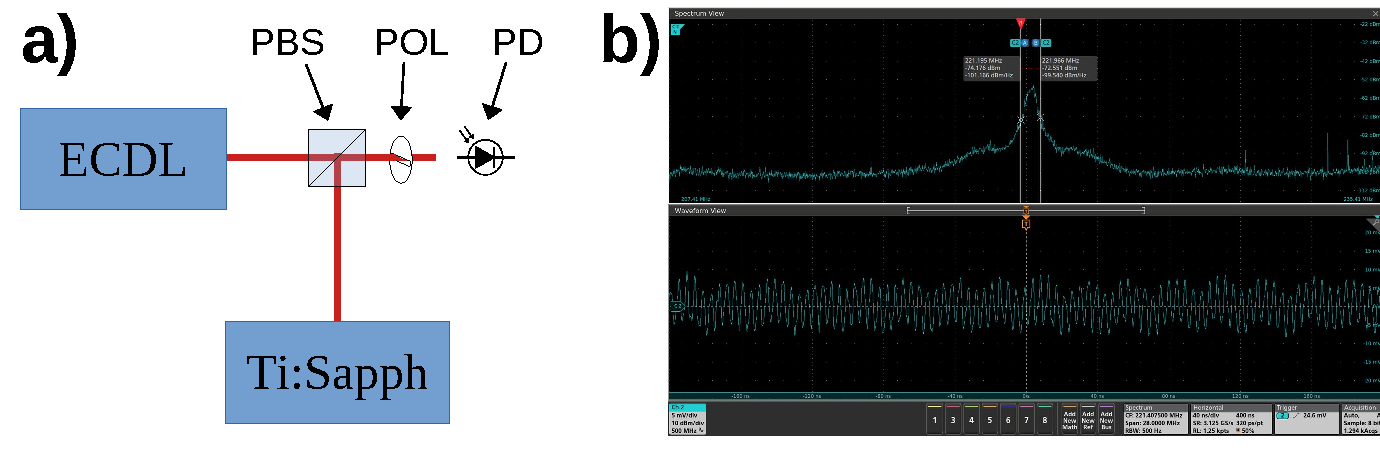
\includegraphics[width=1.0\linewidth]{diagrams/beatNote_cw-cw}
	\caption{Measurement of the optical beat note between two CW lasers. This is done by spatially overlapping the beams in the manner shown in \textbf{a)} using a polarizing beam splitter (PBS) and a polarizer (POL) to project the orthogonal polarizations onto the same axis. The overlapped beams have their intensity value measured by the fast photodiode (PD) which gives a strong oscillating signal when the two CW lasers have their optical frequency very close. The recording of this beat note is shown in \textbf{b)}, where both the time domain and frequency domain traces are shown simultaneously using a Tektronix MSO58 mixed-signal oscilloscope. In the upper portion is the output of the spectrum analyzer which shows an RF peak centered at 221.6 MHz. The lower portion is the time domain trace after the DC offset has been removed. It can be seen that the beat note oscillations are pronounced enough to be counted.}
	\label{fig:wl_beatnote_cw-cw}
\end{figure}

\section{Paraxial Wave Equation and Laser Beam Profiles} \label{sec:paraxial_approx}

The purpose of this section is to develop the Gaussian beam solution to Maxwell’s equations under the paraxial approximation and to introduce the complex $q$-parameter formalism that is essential for understanding optical cavities used in cavity-enhanced absorption spectroscopy techniques such as CRDS and Vernier spectroscopy.

By deriving solutions to the paraxial wave equation, we provide the necessary mathematical basis for the more advanced concepts discussed elsewhere in this dissertation, specifically regarding cavity path-length enhancement and the requirements for precise mode-matching. While the Fresnel integral provides a general method for calculating diffraction, the focus here is on the development of the complex $q$-parameter formalism, which provides a far more compact and physically transparent description of beam propagation that is essential for understanding optical cavities. This approach culminates in the introduction of the ray transfer matrix ($ABCD$) mathematics.

\subsection{Paraxial Wave Equation}
In a vacuum free of charges and currents, the electromagnetic field is governed by the Maxwell wave equation:
\begin{equation}
	\left(\nabla^2 - \frac{1}{c^2}\frac{\partial^2}{\partial t^2}\right)\mathbf{E}(\mathbf{r}, t) = 0
\end{equation}
For monochromatic waves of the form $\mathbf{E}(\mathbf{r},t) = \mathbf{E}(\mathbf{r})e^{-i\omega t}$, this reduces to the homogeneous Helmholtz equation:
\begin{equation} \label{helmholtz}
	\nabla^2 E + k^2 E = 0
\end{equation}
A general solution to the Helmholtz equation can be constructed via the Huygens-Fresnel principle, which treats any aperture as a collection of secondary spherical wavefronts originating from every point on the aperture surface. The field at a distance $d$ is given by the superposition:
\begin{equation}
	E(x,y,z=d) = -\frac{i}{\lambda}\int\int dx' dy' E(x',y',z=0) \frac{e^{i\mathbf{k}\cdot\mathbf{r}}}{R} \left[ \frac{1-\cos(\mathbf{\hat{r}},\mathbf{\hat{z}})}{2}\right]
\end{equation}
where the term in the brackets is the obliquity factor introduced by Kirchhoff to remove backward-travelling waves.

In most laser-based spectroscopic applications, we operate in the Fresnel regime, where the distance from the aperture is much greater than the aperture size itself ($d \gg \sqrt{(x-x')^2 + (y-y')^2}$). In this limit, we can approximate the wavefront as nearly planar ($R \approx d$) and the obliquity factor as unity. This simplifies the propagation to the Fresnel integral:
\begin{equation} \label{fresnel_integral}
	E(x,y,{z=d}) \,=\, \frac{-i}{\lambda d}e^{ikd} e^{\frac{ik}{2d}(x^2+y^2)}\int\int dx' dy' E(x',y',z=0) e^{\frac{-ik}{2d} (x'^2 + y'^2)} e^{\frac{ik}{d} (x x' + y y')}
\end{equation}
While the Fresnel integral provides a powerful method for calculating diffraction patterns, it is computationally intensive. To describe the smooth evolution of a laser beam more efficiently, we seek a streamlined approach by applying the \textit{paraxial approximation} directly to the Helmholtz equation. This yields the Paraxial Wave Equation (PWE), a differential equation that the Fresnel integral satisfies.

We consider a beam that maintains a well-defined direction along the $z$-axis. We use the ansatz
\begin{equation}
	E(\mathbf{r}) = E_0(\mathbf{r}) e^{ikz}
\end{equation}
to distinguish between the rapidly oscillating carrier wave and $E_0(\mathbf{r})$, a slowly varying spatial envelope. Substituting this into (\ref{helmholtz}) yields:
\begin{align}
	\left(\frac{\partial^2}{\partial x^2} + \frac{\partial^2}{\partial y^2} + \frac{\partial^2}{\partial z^2}\right)E_0 e^{ikz} + k^2 E_0 e^{ikz} &= 0 \nonumber\\
	\Bigg[\nabla_{\perp}^2 E_0 + \underbrace{\frac{\partial^2 E_0}{\partial z^2}}_{\mathclap{\begin{matrix}\approx 0\;\mathrm{parax.}\end{matrix}}}
	+ 2ik\frac{\partial E_0}{\partial z} - \cancel{k^2 E_0} + \cancel{k^2 E_0} \Bigg] e^{ikz} &= 0
\end{align}
where $\nabla_{\perp}^2 \equiv \partial^2/\partial x^2 + \partial^2/\partial y^2$. The paraxial approximation is valid when the envelope $E_0$ varies slowly along the direction of propagation, such that $\left|2k\frac{\partial E_0}{\partial z}\right| \gg \left|\frac{\partial^2 E_0}{\partial z^2}\right|$. Neglecting this second-order longitudinal derivative term leads to the Paraxial Wave Equation (PWE):
\begin{equation}\label{parax}
	\nabla_{\perp}^2 E_0 + 2ik\frac{\partial E_0}{\partial z} = 0
\end{equation}

\section{Connection to the Schrödinger Equation}

Through an appropriate change of variables, the paraxial wave equation (\ref{parax}) is mathematically isomorphic to the two-dimensional, time-dependent Schrodinger equation for a particle of mass $m$ (where $z$ plays the role of time) under the influence of an isotropic two-dimensional harmonic oscillator \cite{gaussBeam_schrodinger, diss_Strohaber2007}.

If we factor out a Gaussian dependence of the transverse profile in the form
\begin{equation}
	E_0(x,y,z) = \frac{w_0}{w(z)} f(\zeta,\eta,t)
	\exp\left(\frac{ik r^2}{2R(z)}\right)
\end{equation}
as well as introduce the scaled transverse coordinates $\zeta$, $\eta$, and the choice of the parameter $t'(z)$, analogous to time,
%	\begin{align}
	%		{t'} = \tan^{-1}\left(\frac{z}{z_R}\right) &&
	%		\frac{d{t'}}{dz} = \frac{w_0^2}{w^2 z_R}
	%	\end{align}
\begin{align}
	\zeta = \frac{\sqrt{2}x}{w(z)} &&
	\eta = \frac{\sqrt{2}y}{w(z)} && 
	{t'} = \tan^{-1}\left(\frac{z}{z_R}\right) &&
	\frac{d{t'}}{dz} = \frac{w_0^2}{w^2 z_R}
\end{align}
then the function $f(\zeta, \eta)$ gives the transverse profile of the beam as the Schrodinger equation
\begin{equation}
	\label{schrodinger_form}
	\left(
	\partial_{\zeta\zeta} + \partial_{\eta\eta}
	- \zeta^2 - \eta^2 + 2i\partial_{t'}
	\right) f = 0
\end{equation}

This is formally identical to the Schrödinger equation for a two-dimensional isotropic harmonic oscillator, with ${t'}(z)$ playing the role of time. This mapping allows us to treat the spatial evolution of a laser beam as a temporal evolution of a quantum state. Physically we can think of intercepting a laser beam with a piece of paper and viewing the transverse profile. As we move this paper along the beam propagation direction with a constant velocity, the profile exhibited by the beam on the paper evolves in space just as the 2D quantum harmonic oscillator evolves in time. For well-behaved laser, we excpect this oscillator to be in the ground state.

\subsection{Natural Basis of Beam Description}
The Schrodinger equation (\ref{schrodinger_form}) describing the transverse beam profile $f(\zeta, \eta)$ is separable in the three different coordinate systems \cite{schrodinger_2dho_separability}. These correspond to the fundamental modes of laser propagation.

In Cartesian coordinates, (\ref{schrodinger_form}) becomes separable using the ansatz
\begin{equation}
	f(\zeta,\eta,t) = A(\zeta,t)\,B(\eta,t)
\end{equation}
leads to two identical one-dimensional equations
\begin{equation}
	A_{\zeta\zeta} - \zeta^2 A + 2i A_t = 0
	\qquad
	B_{\eta\eta} - \eta^2 B + 2i B_t = 0
\end{equation}

Focusing on $A(\zeta,t)$ and separating variables in $\zeta$ and $t$, the spatial part satisfies
\begin{equation}
	\frac{d^2 A}{d\zeta^2} - \zeta^2 A + \lambda A = 0
\end{equation}
Which gives physically acceptable solutions as a Gaussian multiplied by a Hermite polynomial $H_n(\zeta)$
\begin{align}
	A(\zeta) = e^{-\zeta^2/2} H_n(\zeta) & & H_n(\zeta) = (-1)^n e^{\zeta^2}\frac{d^n}{d\zeta^n}e^{-\zeta^2}
\end{align}

\subsection{Transverse Mode Structure}

The transverse field distribution is therefore determined by solutions of the Schrodinger equation of the 2D isotropic oscillator. There are three natural basis sets to describe these solutions corresponding to the coordinate systems in which this problem is separable. 

Solutions to the paraxial equation in Cartesian coordinates $(\zeta, \eta)$ yield Hermite-Gaussian modes
\begin{equation}
	E_{nm}(x,y,z) \propto H_n(\text{scaled } x)H_m(\text{scaled } y)\exp(-\text{Gaussian envelope})
\end{equation}
while cylindrical $(r, \theta)$ coordinates yield Laguerre-Gaussian modes
\begin{equation}
	E_{pl}(r,\theta,z) \propto L_p^l(\text{scaled } r)\exp(il\theta)\exp(-\text{Gaussian envelope})
\end{equation}
Laguerre-Gaussian modes carry orbital angular momentum (OAM), while Hermite-Gaussian modes form a convenient basis for rectangular symmetry.

In this work, these higher-order modes are primarily relevant in the context of cavity alignment and mode-matching. Usually this misalignment occurs in the Cartesian directions, as opposed to some circularly varying phase delay. Therefore, the Hermite-Gauss modes form a natural basis for describing this misalignment. Efficient coupling into an optical cavity requires excitation of the fundamental $\mathrm{TEM}_{00}$ Gaussian mode; coupling into higher-order HG modes represent a rectangular misalignment of the cavity or input beam, leading to reduced coupling efficiency. For the purposes of cavity enhancement and mode-matching, we can therefore focus on the evolution of the Gaussian envelope itself. The Gaussian beam corresponds to the lowest-order HG solution ($n=m=0$), while higher-order modes arise as excited states of the same underlying Schrödinger-like system.

This formulation makes clear that the Gaussian beam is the fundamental, minimum-divergence solution of the paraxial wave equation (the isotropic oscillator only has one ground state solution, a Gaussian), and that higher-order transverse modes form a complete orthogonal basis determined by the symmetry of the coordinate system.

\section{Gaussian Beam Solution}

The fundamental TEM$_{00}$ solution to the paraxial equation is the Gaussian beam
\begin{equation} \label{gauss_TEM00}
	E_0(r,z) \propto \frac{w_0}{w(z)} \exp\left(-\frac{r^2}{w^2(z)}\right)
	\exp\left(i\frac{kr^2}{2R(z)} - i\psi(z)\right),
\end{equation}
It is convenient to make the identification of the following parameters, as they will be used frequently throughout this work
\begin{itemize}
	\item $w(z)$ is the \textbf{beam radius} at any location $z$ along the beam propagation direction
	\item $R(z)$ is the \textbf{wavefront radius of curvature}
	\item $\psi(z)$ is the \textbf{Gouy phase}
	\item $z_\mathrm{R}$ is the \textbf{Rayleigh range}, determined by the size of the beam waist
\end{itemize}
For a beam which comes to a focus at $z=0$, where $w(0) = w_0$ is the size of this waist, these quantities are respectively given by
\begin{align}
	w(z) &= w_0 \sqrt{1 + \left(\frac{z}{z_R}\right)^2} \\
	R(z) &= z\left[1 + \left(\frac{z_R}{z}\right)^2\right] \\
	\psi(z) &= \tan^{-1}\left(\frac{z}{z_R}\right) \\
	z_\mathrm{R} &= \pi n_r w_0^2/\lambda
\end{align}

Although the refractive index $n_r$ makes an appearance in the expression for $z_\mathrm{R}$, we will treat this as always being close to unity $n_r\simeq 1$, as the transition between media of differing refractive indices will be unimportant for this work.

\section{The Complex $q$-Parameter and Laser Beam Profile}

For a beam having a fundamental $\mathrm{TEM}_{00}$ solution with waist located at $z=0$, the field can be expressed compactly using the complex parameter $q(z)$:
\begin{equation}\label{gauss_TEM00-q}
	E_0(r,z) = E_0 \frac{w_0}{w(z)} \exp\left( -\frac{r^2}{w^2(z)} \right) \exp\left( i \left[ k z + \text{arg}(q(z)) \right] \right)
\end{equation}
where the phase evolution is intrinsically linked to the argument of $q$. Rather than treating $w(z)$ and $R(z)$ separately, it is convenient to define the complex beam parameter
\begin{equation}\label{complex_q}
	q(z) = z + i z_R.
\end{equation}
where its reciprocal encodes both geometric properties
\begin{equation} \label{compex_q_recip}
	\frac{1}{q(z)} = \frac{1}{R(z)} - \frac{i\lambda}{\pi n_r w^2(z)}.
\end{equation}

The utility of the complex $q$-parameter lies in its ability to encode the entire transverse state of a Gaussian beam into a single complex scalar via the  intensity profile $w(z)$ and the phase front curvature $R(z)$. Because the $1/q$ relation maps the physical properties of the beam onto the real and imaginary parts of a complex value, any linear optical transformation that affects the beam's geometry can be expressed as a transformation of $q$. For this work, we will use the vacuum refractive index $n_r = 1$.

\subsection{Ray Transfer Matrix Formalism}

The propagation of a Gaussian beam through an optical system can be represented by a single effective matrix $\mathbf{M}$ constructed from the product of individual element matrices:
\begin{equation}
	\begin{pmatrix} A & B \\ C & D \end{pmatrix} = \mathbf{M}_n \dots \mathbf{M}_2 \mathbf{M}_1
\end{equation}
The transformation of the $q$-parameter through such a system is given by the Möbius transformation:
\begin{equation} \label{gauss_complex_q_ABCD}
	q_{\text{out}} = \frac{Aq_{\text{in}} + B}{Cq_{\text{in}} + D}
\end{equation}
This formulism is convenient for the next chapter, where we will apply these matrices to determine the stability and eigenmode properties of the optical cavities used for ultra-sensitive absorption measurements.

\subsubsection{Ray Optical Analogy}
In classical ray optics, the propagation of a light ray through a system of lenses and mirrors is also described by the ray transfer matrices \cite{book_lasers_siegman} which take the same form as the $ABCD$ matrices. These track the evolution of a ray's position ($x$) and angle ($\theta$) from the optical axis through interactions in an optical system. Since a Gaussian beam can be similarly be viewed as a collection of rays concentrated around the optical axis (see Eq. \ref{fresnel_integral}), it is natural to ask how the $q$-parameter evolves when subjected to these same linear transformations.

The transition from the physical parameters $R(z)$ and $w(z)$ to the matrix formalism is made seamless by recognizing that the ray transfer $ABCD$ matrix acts on the complex $q$-parameter through a fractional linear transformation (or Möbius transformation). This allows us to bypass the cumbersome tracking of $R(z)$ and $w(z)$ through every lens and mirror in a complex setup, instead treating the entire optical train as a single operator acting on the initial beam state.

Consider how a single optical element transforms the transverse geometry of the beam. In ray optics, the state of a ray is defined by its distance $x$ and $\theta$ from the $z$-axis. For a paraxial ray ($\theta\sim0$), the transformation through an element $\mathbf{M}$ is:
\begin{align}
	\begin{pmatrix} x_{\text{out}} \\ \theta_{\text{out}} \end{pmatrix} = \begin{pmatrix} A & B \\ C & D \end{pmatrix} \begin{pmatrix} x_{\text{in}} \\ \theta_{\text{in}} \end{pmatrix}
\end{align}
The complex $q$-parameter is related to the ray's wavefront curvature. Specifically, for a beam propagating along $z$, the phase term $\exp(ikx^2/2R)$ in (\ref{gauss_TEM00}) implies that the angular divergence of the rays at the beam axis is intrinsically linked to the derivative of this phase.

The action of the $ABCD$ matrix on the complex $q$-parameter via Eq. (\ref{gauss_complex_q_ABCD}) represents a linear transformation of the underlying ray-optical phase-space coordinates $(x, \theta)$. In this representation, the real and imaginary parts correspond to the beam's wavefront curvature ($1/R$) and its transverse area ($\propto 1/w^2$). The $ABCD$ matrix acts on these components such that the "area" in this complex space--the product of the curvature and the beam area, $R \cdot w^2$--is conserved. This is a direct manifestation of Liouville’s theorem; the phase space volume preserves the fundamental structural relationship between the beam's divergence and its waist. Consequently, the unimodular constraint
\begin{equation}
	\det \mathbf{M} = 1
\end{equation}
ensures that while the beam may expand or contract, the quadratic phase structure required to maintain a Gaussian profile remains intact throughout propagation.

\section{Stable Optical Cavity Geometry}
A fundamental application of this formalism is the description of optical cavities. In a cavity, the field must be self-consistent; that is, the Gaussian beam describing the intracavity field must remain invariant after a single round trip. Using the $ABCD$ law (\ref{gauss_complex_q_ABCD}), this condition is expressed as a fixed-point equation for the complex beam parameter
\begin{equation} \label{cav_eigenvalue}
	q = \frac{Aq + B}{Cq + D}
\end{equation}
Solutions to this equation define the cavity eigenmodes. To investigate the stability of such a system, it is computationally convenient to solve for the reciprocal of the complex $q$-parameter. By forming $1/q$ in the fixed-point relation (\ref{cav_eigenvalue}), we can reformulate the stability condition as a quadratic equation
\begin{equation}
	B\left(\frac{1}{q_\mathrm{eig}}\right)^2 + (A-D)\left(\frac{1}{q_\mathrm{eig}}\right) - C = 0
\end{equation}
This gives two solutions for the reciprocal of the complex q-parameter of the cavity eigenmode
\begin{equation}
	\frac{1}{q_\mathrm{eig}} = \frac{D-A}{2B} \pm \frac{1}{B}\sqrt{\frac{(D-A)^2}{4} + BC}
\end{equation}
The solution is chosen such that the imaginary part is negative to agree with (\ref{compex_q_recip}). Using the unimodularity condition $AD - BC = 1$, we then have for the complex $q$-parameter of the cavity eigenmode
\begin{equation} \label{cavity_eigenmode_recip}
	\frac{1}{q_\mathrm{eig}} = \frac{A-D}{2B} - \frac{i}{|B|}\sqrt{1 - \frac{1}{4}\left(D + A\right)^2}
\end{equation}
The waist size and location can be determined by equating the real and imaginary parts of (\ref{complex_q}) to those of $q_\mathrm{eig}$. While these can be found by taking the reciprocal of above for $1/q_\mathrm{eig}$, it is much easier to re-arrange the quadratic equation (\ref{cav_eigenvalue}) to give $cq_\mathrm{eig}^2 + (D-A)q_\mathrm{eig} -B = 0$, and the solution
\begin{equation}\label{cavity_eigenmode}
	q_\mathrm{eig} = \frac{A-D}{2C} + \frac{i}{|C|}\sqrt{1-\frac{1}{4}(D+A)^2}
\end{equation}
The stability of the cavity--the condition that a physical, finite beam waist exists--requires that the term under the radical remains positive. This yields the fundamental stability criterion for an optical cavity
\begin{equation} \label{cavity_stab_condition}
	\left|D+A\right| \leq 2
\end{equation}
where the values of $A$ and $D$ come from the round-trip $ABCD$ ray transfer matrix.

\section{ABCD Matrices of Cavity Elements and Configurations}
The configuration of mirrors and non-refractive focusing optics common in the construction of cavities are represented by the ray-transfer $ABCD$ matrices	
\begin{itemize}
	\item Free Space Propagation
	\begin{equation} \label{mat_prop}
		\mathbf{P}_d = 
		\begin{pmatrix}
			1 & d \\
			0 & 1
		\end{pmatrix}
	\end{equation}
	\item Flat Mirror Reflection
	\begin{equation*}
		\mathbf{M} = 
		\begin{pmatrix}
			1 & 0 \\
			0 & 1
		\end{pmatrix}
	\end{equation*}
	\item Curved Mirror Reflection
	\begin{equation*}
		\mathbf{M}_R = 
		\begin{pmatrix}
			1 & 0 \\
			-\frac{2}{R} & 1
		\end{pmatrix}
	\end{equation*}
\end{itemize}

For the optical cavities considered in this work, the beam does not cross any refractive index boundaries in the cavity round-trip. Due to Fresnel reflections, this is usually to be avoided. For this reason, we have considered the refractive index throughout this work to be unity $n_r = 1$. While refractive index boundaries can be effectively modeled using the ray-transfer matrix formulism, it should be pointed out that there are effectively two different approaches for the propagation of a Gaussian beam:
\begin{itemize}
	\item Using a ray transfer matrix to explicitly show the change in direction across the boundary having ratio of refractive indices $n$. This is the diagonal ABCD matrix having $A=1$ and $D=1/n$, which is equivalent to the transformation $q' = nq$. The beam radius calculation must then undo this transformation by $w' = w/ \sqrt{n}$.
	
	\item Transform all propagation distances inside the medium by an amount $d' = d/n$.
\end{itemize}

\noindent
Such considerations may be used, for instance, in the atigmatic compensation of ring cavities, where the inclusion of a Brewster-angled refractive element can compensate for the astigmatism introduced by the angled focusing mirrors \cite{book_ultrashort_lp_phenom_CH5}. For the remainder of this work, however, we will take the refractive index to be that of the vacuum without any refractive index boundaries. 

\subsection{Linear Optical Cavity} \label{sec:cav_ABCD}
The simplest linear optical cavity consists of two mirrors separated by a distance $L$, as in Fig. \ref{fig:cavitylinear}. We will later show how a small absorption can be greatly amplified using an optical cavity. This absorption signal manifests itself as a change in the round-trip loss. A cavity which has low intrinsic losses is then naturally able to measure small changes in intra-cavity absorption. When the mirror reflectivity is the limiting factor in this round-trip loss, the number of reflections should be minimized. The simple linear cavity has the fewest number of reflections.

\begin{figure}[H]
	\centering
	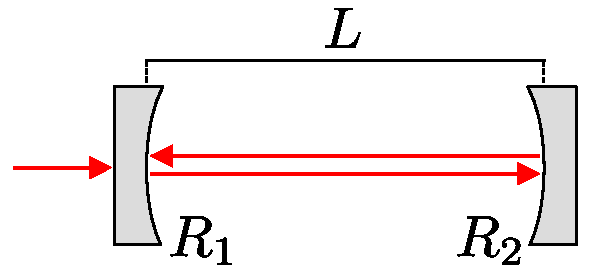
\includegraphics[width=0.3\linewidth]{diagrams/cavity_linear}
	\caption{Simple linear optical cavity constructed from two mirrors having radii of curvature $R_{1,2}$ and separation distance $L$.}
	\label{fig:cavitylinear}
\end{figure}

We consider a cavity consisting of two mirrors having radii of curvature $R_1$ and $R_2$ separated by a distance $L$. Using the ray transfer matrices (\ref{mat_prop}), we represent the propagation from one mirror to the other as the matrix $\mathbf{P}_L = \begin{pmatrix} 1 & L \\ 0 & 1 \end{pmatrix}$ and the mirror reflections as $\mathbf{M}_{1,2} = \begin{pmatrix} 1 & 0 \\ -2/R_{1,2} & 1 \end{pmatrix}$. Starting from the mirror having curvature $R_1$, the $ABCD$ matrix representing the round trip of the cavity is
\begin{equation}
	\begin{pmatrix}
		A & B \\
		C & D
	\end{pmatrix}
	=
	\mathbf{M}_1 \, \mathbf{P}_L \, \mathbf{M}_2 \, \mathbf{P}_L
\end{equation}
The coefficients of the resulting transfer matrix are
\begin{align}
	A &= 1 - \frac{2L}{R_2} & 
	B &= L\left(2 - \frac{2L}{R_2}\right) \\
	C &= -\frac{2}{R_2} + \frac{2}{R_1}\left(\frac{2L}{R_2} - 1\right) & 
	D &= 1- \frac{2L}{R_2} - \frac{2L}{R_1}\left(2 - \frac{2L}{R_2}\right)
\end{align}
If we introduce the dimensionless parameter $g_{1,2} = 1 - L/R_{1,2}$, then the matrix elements become
\begin{align}
	A &= 2g_2-1 & B &= 2Lg_2 \\
	C &= \frac{2}{L}\left(2g_1g_2 - g_1 - g_2\right) & D &= 4g_1g_2 - 2g_2 -1
\end{align}
The stability condition $\left|A + D\right| \leq 2$ then reads
\begin{align}
	-2 \leq 4g_1g_2 - 2  \leq 2 \nonumber \\
	0 \leq g_1 g_2 \leq 1 \nonumber
\end{align}
The stability condition for the linear cavity can then be written as
\begin{equation}
	0 \leq \left(1 - \frac{L}{R_1}\right)\left(1 - \frac{L}{R_2}\right) \leq 1
\end{equation}

We can retrieve the beam radius at one of the mirrors by equating the imaginary part of (\ref{compex_q_recip}) to that of (\ref{cavity_eigenmode_recip}). The beam radius at mirror $R_1$ is then
\begin{align} \label{cavity_beamsize_m1}
	w_1^2 = \frac{\lambda}{\pi n} \Big/ \left(\frac{1}{|B|}\sqrt{1 - \frac{1}{4}(D+A)^2}\right)
	&= \frac{\lambda L}{\pi n}\sqrt{\frac{g_2}{g_1(1-g_1g_2)}}
	%\sqrt{\frac{\frac{\lambda}{\pi n}L(L-R)}{R_2\sqrt{L\left(1 - \frac{L}{R_1}\right)\left(1-\frac{L}{R_2}\right)\left(\frac{1}{R_1} + \frac{1}{R_2} - \frac{L}{R_1R_2}\right)}}}
\end{align}
We can repeat the computation for the round-trip ABCD matrix, but instead starting at mirror $R_2$. The new ABCD matrix would be the same, expect for the swapped $g_1 \leftrightarrow g_2$. With this in mind, we can immediately write the beam radius at mirror $R_2$ as
\begin{equation} \label{cavity_beamsize_m2}
	w_2^2 = \frac{\lambda L}{\pi n}\sqrt{\frac{g_1}{g_2(1-g_1g_2)}}
\end{equation}

When trying to mode-match an input beam to the cavity, it is useful to know the location of the beam waist and its size $w_0$. These are conveniently related through (\ref{complex_q}) to the cavity eigenmode. It can be easily seen that the waist size is given by
\begin{align} \label{cavity_w0}
	w_0^2 = \frac{\lambda}{\pi n}\mathrm{Im} \left[q_\mathrm{eig}\right] = \frac{\lambda}{\pi n} \frac{1}{|C|}\sqrt{1-\frac{1}{4}(D+A)^2} = \frac{\lambda L}{\pi n}\frac{\sqrt{g_1 g_2 (1-g_1g_2)}}{\left|2g_1g_2 - g_1 - g_2\right|}
\end{align}
The location of this waist relative to the position of mirror $R_1$ is simply the negative real part of the q-parameter for the cavity eigenmode
\begin{equation} \label{cavity_z0}
	z_0 = -\mathrm{Re}\left[q_\mathrm{eig}\right] = \frac{D-A}{2C} = L\frac{g_2(g_1 - 1)}{2g_1g_2 - g_1 - g_2}
\end{equation}

\subsubsection{Half-Symmetric Cavity}
A useful configuration for an optical cavity is the half-symmetric cavity, which has a flat mirror and a curved mirror having radius of curvature $R$. If we consider that the cavity round-trip is starting at the flat mirror, then according to our convention above we have
\begin{eqnarray}
	g_1 = 1 &\qquad& g_2 = 1 - \frac{L}{R} \equiv g
\end{eqnarray}
The location of the beam waist relative to the flat mirror is given by (\ref{cavity_z0}) and can be seen to be $z_0=0$. This means that the beam waist is located exactly at the flat mirror. The size of this waist is given by (\ref{cavity_w0}) and is given by
\begin{equation} \label{cavity_waste_size_half-sym}
	w_{0,\mathrm{HS}} = \frac{\lambda L}{\pi n}\sqrt{\frac{g}{1-g}}
	%= \frac{\lambda L}{\pi n}\frac{\sqrt{(1-L/R) (L/R)}}{\left|-L/R\right|}
	= \frac{\lambda L}{\pi n}\sqrt{\frac{R}{L}-1}
\end{equation}
The stability condition is easily seen to be $R > L$ for the half-symmetric cavity.

\subsection{Mode-Matching} \label{sec:mode-matching}
The most efficient coupling of a laser beam into an optical cavity is achieved by ensuring that the transverse profile of the beam matches the profile of the cavity eigenmode predicted by (\ref{cavity_eigenmode}). The fundamental $\mathrm{TEM}_{00}$ mode of the cavity has a Gaussian profile, and therefore the input beam should be free of higher order spatial modes. For lasers which have a poor beam profile, a spatial mode filter can be employed to clean up the beam at the expense of power. Once a clean Gaussian beam is achieved, it can be profiled using the knife-edge technique \cite{book_gaussBeams_AtomsMolsOpticalPhys2} or other beam profiling method. The ray transfer matrices (\ref{mat_prop}) can then be used to find a set of focusing elements which bring the laser beam profile into overlap with the cavity eigenmode.

We gave as an example the half-symmetric cavity, having a flat mirror as an input coupler and a curved mirror of radius $R$. We found that the cavity eigenmode has a waist which is located at the flat mirror with radius $w_0$ given by (\ref{cavity_waste_size_half-sym}). From equation (\ref{gauss_complex_q_ABCD}), we have the complex $q$-parameter $q(z)$ at every location $z$ in the cavity. From (\ref{compex_q_recip}), we find that the transverse profile of the beam follows the hyperbola
\begin{equation} \label{beam_hyperbola}
	w(z) = \sqrt{\frac{-\lambda}{\pi n \,\mathrm{Im} \left[\frac{1}{q(z)}\right]}} = w_0\sqrt{\left(\frac{z}{\pi n w_0^2 /\lambda}\right)^2 + 1}
\end{equation}
If the flat mirror is located at $z=0$ and the curved mirror is located at $z=L$, then the profile of the input beam must match what is predicted by the above equation for negative $z$ values. The profile of the input beam which is matched to a half-symmetric cavity is shown in Fig. \ref{fig:cavitymodematch}(a), where the cavity eigenmode is calculated using the parameters $L=1200$mm and $R=2000$mm.

In general, the input beam must match the cavity eigenmode extrapolated past the input coupler. A more complicated ring cavity configuration is shown in Fig. \ref{fig:cavitymodematch}(b), where the cavity eigenmode is seen to form two waists. The input beam profile can be calculated from equation (\ref{beam_hyperbola}) using the correct beam waist location and size.

\begin{figure}[H]
	\centering
	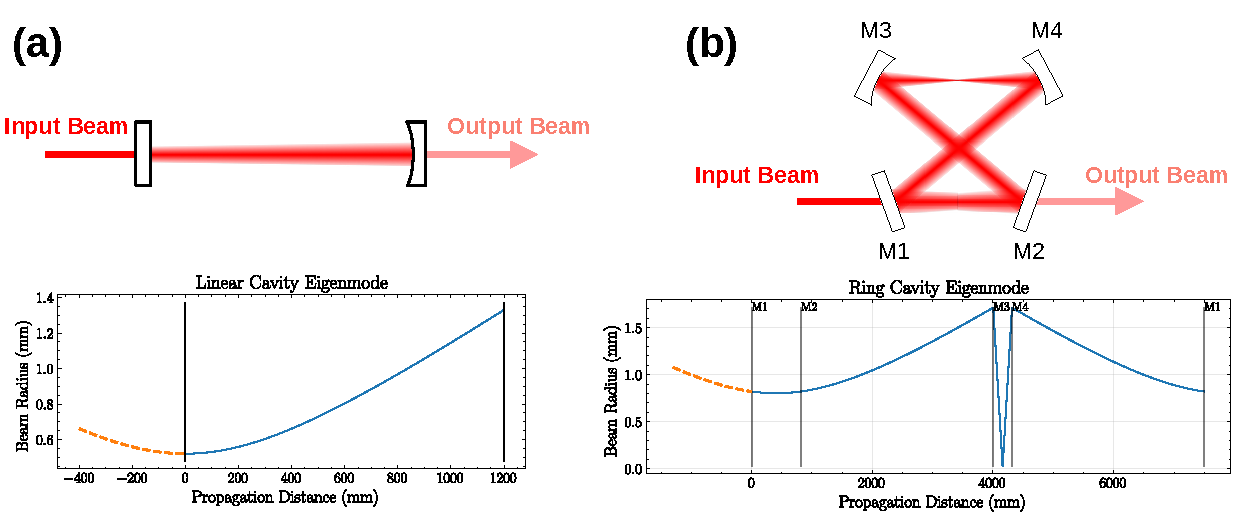
\includegraphics[width=1.0\linewidth]{diagrams/cavity_modeMatch}
	\caption{Shown are the calculated eigenmodes for two optical cavity configurations used in this work. The blue traces in the lower panes corresponds to the cavity eigenmode, and the dashed orange trace corresponds to the modematched input beam. For the half-symmetric linear cavity shown in \textbf{(a)}, the input coupler is a flat mirror and the waist of the eigenmode sits at the reflective surface. The output coupler is a curved mirror of radius $R=2$m located a distance $L=1.2$m away from the input coupler, and the wavefront radius of curvature of the eigenmode matches this value at the reflective interface. Shown in \textbf{(b)} is a ring cavity having the shown simplified configuration. Mirrors M1 and M2 are the flat input and output couplers. Mirrors M3 and M4 are concave mirrors having radius of curvature $R=300$mm. The eigenmode for this cavity forms two waists, one of tight focus halfway between the concave mirrors and another which is located away at one half the round trip distance of the cavity. The total length of the cavity gives $\mathrm{FSR} \sim 40\mathrm{MHz}$.}
	\label{fig:cavitymodematch}
\end{figure}

It should be noted that the linear cavity shown in Fig. \ref{fig:cavitymodematch}(a) has the property that the condition for mode-matching corresponds exactly to maximum back-reflectance of the input beam from the furthest mirror back into the laser source. For this reason, it is advised to use a form of optical isolator between the laser and a linear cavity to prevent this maximally back-reflected beam from entering back into the laser source. The ring cavity does not have this issue, since the beam returning from the cavity round-trip is pointing in a different direction than the input beam.	


\chapter{OPTICAL CAVITY DYNAMICS} \label{chap:cav_dynamics}

The practical application of cavity-enhanced spectroscopy relies on understanding how optical cavity systems respond to time-dependent perturbations. In applications such as Cavity Ring-Down Spectroscopy (CRDS) and Vernier spectroscopy, the experimental signal is not merely a steady-state transmission, but a complex transient response resulting from the dynamic interaction of cavity length and laser wavelength.

This chapter develops the mathematical framework required to model these dynamic interactions. We begin by deriving the steady-state Airy transmission function for a monochromatic input, establishing the fundamental relationships between cavity finesse, free spectral range (FSR), and resonance linewidth. Subsequently, we transition to the time domain, treating the cavity as a linear system characterized by a specific impulse response. Finally, we establish the theoretical basis for the transient decay models employed in this work by analyzing the convolution of this impulse response with various input waveforms, including rectangular pulses, frequency-swept signals, and length-modulated transients.

Ultimately, these derivations provide the analytical tools necessary to interpret the high-speed photodetector signals discussed in the other chapters, where these dynamic cavity responses are leveraged for the ultra-sensitive detection of trace molecular species in breath analysis applications.

\section{Steady State Intensity Transmitted by an Optical Cavity} \label{sec:cav_transmission}
We consider here monochromatic light incident on a stable optical cavity having length $L$ with input coupler located at $z=0$. The incoming light has Gaussian transverse profile $E_0(x,y,z)$, and we write the incident electric field as
\begin{equation}
	E_\mathrm{in}(x,y,z,t) = E_0(x,y,z) e^{i\omega t - kz}
\end{equation}
From the discussion in Sec. \ref{sec:paraxial_approx}, the transverse profile $E_0(x,y,z)$ obeys the paraxial wave equation (\ref{parax}) and therefore evolves as a Gaussian beam between the cavity mirrors.

For now we will assume perfect mode-matching where the transverse profile of the input beam has complex-$q$ parameter that matches the cavity eigenmode (\ref{cavity_eigenmode}) at the input coupler. It is then understood that the transverse profile at the output of the cavity $E_0(x,y,z=L)$ is that of a Gaussian beam having beam size (\ref{cavity_beamsize_m2}) with a waist of size (\ref{cavity_w0}) located a distance (\ref{cavity_z0}) from the input coupler. For a symmetric cavity the transverse profile of the output field exactly matches that of the input field.

For a more general cavity, the transverse field at a single point $E_0(x,y,0)$ on the input coupler is mapped to a corresponding point on the output coupler by a complex constant $E_0(x,y,L) = a(x,y)E_0(x,y,0)$. For the remainder of this section, we will only be concerning ourselves with the time dependence of a photodetector which is reading the intensity of the light integrated across the transverse profile of the beam. Since the integrated intensity is unaffected by the beam size, equivalent to the condition $\int\int\left(\left|a(x,y)\right|^2 -1\right)\left|E_0(x,y,0)\right|^2 dx dy = 0$, we will simply take $a=1$ with the understanding that the detailed transverse profile at the output coupler has additional complex factor in front which does not affect the integrated intensity for non-symmetric cavities.

As shown in Fig \ref{fig:cavitytransmission}b, the incident light makes a single pass through the cavity encountering two mirror transmissions and a phase factor from the distance $L$ of propagation. The mirrors are characterized by their reflection coefficient $r$ and transmission coefficient $t$, which give the transmitted and reflected electric field as $tE$ and $rE$, respectively, as shown in Fig. \ref{fig:cavitytransmission}a. In general these coefficients are complex, allowing for a phase shift of the field in transmission and reflection. This contributes part of the output as $E_\mathrm{in} t^2 e^{-i\omega L/c}$. At the second cavity mirror, the single pass beam is reflected twice and encounters a phase factor from the $2L$ propagation distance giving an additional output of $E_\mathrm{in} t^2 e^{-i\omega L/c} r^2 e^{-2i\omega L/c}$. The total output of the cavity is the sum of the infinitely many contributions from successive number of round trips.
\begin{figure}[H]
	\centering
	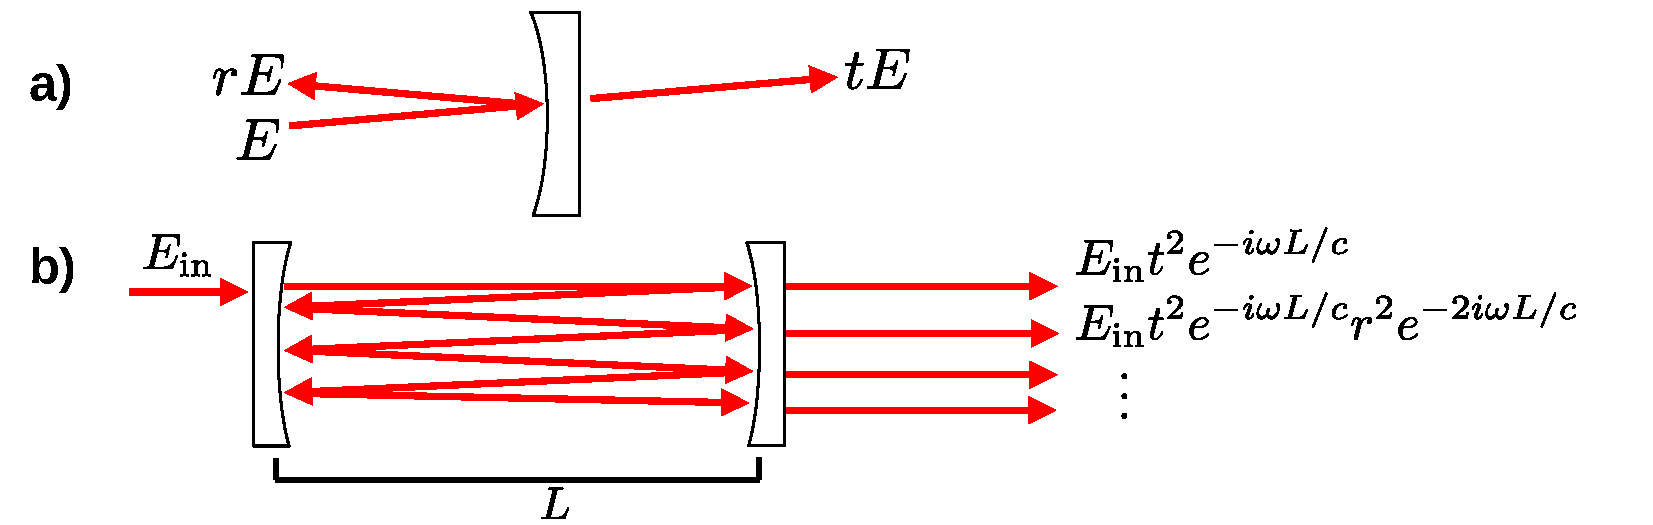
\includegraphics[width=0.7\linewidth]{diagrams/cavityTransmission}
	\caption{In \textbf{a)} is shown the complex coefficients of reflection $r$ and transmission $t$ which act to attenuate and phase shift the incident wave having field $E$. In \textbf{b)} the process of summing the many cavity round trips is illustrated. The output of the cavity is a sum of the single pass and the infinitely many round trips.}
	\label{fig:cavitytransmission}
\end{figure}

The output of the cavity is given by the sum
\begin{align} \label{cav_E-sum}
	E_\mathrm{out}(\omega) &= E_\mathrm{in}(\omega) t^2 e^{-i\omega L/c} \sum_{m=0}^\infty r^{2m} e^{-2im\omega L/c} \nonumber \\
	&=E_\mathrm{in}(\omega)\frac{t^2 e^{-i\omega L/c}}{1-r^2 e^{-i\omega t_r}}
\end{align}
In writing the above expression we have used the geometric series $\sum_{m=0}^\infty x^m = 1/(1-x)$, which is valid since $\left|r\right| < 1$ by definition. We have also defined the round-trip traversal time of the cavity $t_r = 2L/c$. The time-averaged intensity seen by a photodetector is given by $E_\mathrm{out}^* E_\mathrm{out}$.
\begin{equation} \label{_cav_I_comp}
	I_\mathrm{out} = I_\mathrm{in} \frac{T^2}{\left|1 - r^2 e^{-i\omega t_r}\right|^2}
\end{equation}
Above we have defined the coefficient $T$ for transmitted light intensity as $\left|t\right|^2 = T$. The complex number $r^2$ is written in terms of a real-valued intensity reflectivity value $R$ and a round-trip phase shift $2\phi$ of the twice reflected electric field
\begin{equation} \label{cav_R_defin}
	r^2 = Re^{-2i\phi}
\end{equation}
The denominator term of (\ref{_cav_I_comp}) is real and this can be reflected switching from complex exponentials to the trigonometric functions
\begin{equation}
	\left|1 - R e^{-i\omega t_r - 2\phi}\right|^2 = 1 + R^2 - 2R\cos(\omega t_r + 2\phi) = (1-R)^2 + 4R\sin^2(\frac{\omega t_r}{2} + \phi)
\end{equation}
We then arrive at the well known Airy formula for the transmitted light Intensity
\begin{equation}\label{cav_airy}
	I_\mathrm{out}(\omega) = \frac{T^2}{(1-R)^2}\frac{1}{1 + \frac{4R}{(1-R)^2}\sin^2\left(\frac{\omega t_r}{2} + \phi\right)} I_\mathrm{in}(\omega)
\end{equation}
The transmission function is a set of evenly spaced resonances when there is no frequency dependence of the reflection phase shift $\phi$. The maximum transmission occurs when the argument to the sine function is an integer multiple of $\pi$, so we have for integer $m$
\begin{align} \label{cav_resonance_condition}
	\frac{\omega L}{c} + \phi(\omega) = m \pi
\end{align}
If we solve for the cavity length $L$ in terms of the wavelength, the mirror separations which give resonance with a laser of wavelength $\lambda$ are evenly spaced in half-integer multiples of this wavelength
\begin{align} \label{cav_resonance_length}
	L = \frac{1}{2}\left(m - \frac{\phi(\lambda)}{\pi}\right)\lambda
\end{align}
The free spectral range (FSR) is given by the spacing of these resonances. For $\phi(\omega)$ being constant between the two resonances, the FSR is given in the optical frequency $\nu$ by
\begin{equation}
	\mathrm{FSR} = \frac{1}{t_r}
\end{equation}
The FWHM width of each resonance in the cavity transmission function (\ref{cav_airy}) is easily found to be
\begin{equation}
	\Delta \nu = \frac{2}{\pi t_r} \sin^{-1}\left(\frac{1-R}{2\sqrt{R}}\right)
	\sim \frac{1}{\pi t_r}\frac{1-R}{\sqrt{R}}
\end{equation}
Note that the above expression is the FWHM in the optical frequency $\nu$, as opposed to the earlier expressions using the angular frequency $\omega = 2\pi \nu$. The approximation made on the right of the expression above is valid for cavity mirrors having high reflectivity $R\sim 1$. In this limit, the cavity resonances look approximately like a Lorentzian near the transmission peak with the resonances becoming narrower for larger reflectivity. We can also define the cavity finesse as the ratio of the free spectral range (FSR) to the width of the resonance
\begin{equation}
	\mathcal{F} = \frac{\mathrm{FSR}}{\Delta\nu} = \pi \frac{\sqrt{R}}{1-R}
\end{equation}
This dimensionless parameter is a sort of quality factor which is only determined by round-trip loss of the field inside the cavity. This sensitivity to the loss can be exploited in cavity mode-width spectroscopy \cite{crds_cavityModeWidth_Cygan} to detect intracavity absorption.

\section{Ring-down Time}
For an optical cavity of sufficiently low loss, it is possible to observe the "ring-down" of light trapped between the mirrors after the laser coupling energy into the cavity has been shut off. This occurs because the light circulating between the mirrors propagates at a finite speed and takes a measurable amount of time for the light to leak out of the cavity mirrors. The response of the cavity to an arbitrary time dependent field is given, and then approximations are made for the case where the input field takes the form of a short pulse. This allows us to derive an analytic expression for the characteristic time of cavity ring-down.

The cavity response in equation (\ref{cav_E-sum}) is linear in the input field and takes the form of a transfer function $E_\mathrm{out}(\omega) = E_\mathrm{in}(\omega) H(\omega)$ in frequency space. The response of the cavity to an arbitrary input electric field $E_\mathrm{in}(t)$ is then the convolution with the inverse Fourier transform of the transfer function $\tilde{H}(t) = \mathcal{F}^{-1}(H(\omega))(t)$, giving
\begin{align} \label{cav_convolution}
	E_\mathrm{out}(t) = \int_{-\infty}^{\infty} E_\mathrm{in}(t-\tau) \tilde{H}(\tau) d\tau &&;&&
	\tilde{H}(t) = \frac{1}{2\pi}\int_{-\infty}^{\infty} e^{i\omega t}H(\omega) d\omega
\end{align}

We wish to find the response of the cavity to an impulsive input. From (\ref{cav_E-sum}) the transfer function is
\begin{equation}
	H(\omega) = T e^{-i\omega t_r/2} \sum_{m=0}^\infty r^{2m} e^{-im\omega t_r}
\end{equation}
Taking the transform of this expression is most easily done in this summation form. For a Dirac delta function input pulse, the output field is simply the impulse response $E_\mathrm{out}(t) = \tilde{H}(t)$. Taking the transform of the above expression and interchanging the sum and integrals
\begin{align} \label{cav_impulse_response}
	\tilde{H}(t)
	&= \frac{T}{2\pi} \sum_{m=0}^\infty r^{2m} \int_{-\infty}^{\infty} e^{i\omega t} e^{-i\omega t_r/2 -im\omega t_r} d\omega \\
	&= \frac{T}{2\pi} \sum_{m=0}^\infty \left(Re^{-2i\phi}\right)^{m}\int_{-\infty}^{\infty} e^{i\omega (t - t_r/2 - m t_r)} d\omega \\
	%&= T \sum_{m=0}^\infty R^{m} \delta(t - t_r/2 - m t_r) \\
	E_\mathrm{out}(t) &= T \sum_{m=0}^\infty \left(Re^{-2i\phi}\right)^{m} \delta(t - t_r/2 - m t_r)
\end{align}

The intensity of the cavity output light is proportional to $E^*_\mathrm{out} E_\mathrm{out}$, which gives
\begin{align}
	I_\mathrm{out}(t) &= T^2 \sum_{m=0}^\infty\sum_{n=0}^\infty R^{m+n} \delta(t - t_r/2 - m t_r)\delta(t - t_r/2 - n t_r) \nonumber \\
	&= T^2 \sum_{m=0}^\infty R^{2m} \delta^2(t - t_r/2 - m t_r)
\end{align}
We note that the second line is obtained by observing that the only non-zero terms of the nested sum are those for which $m=n$ due to the product of delta functions. This takes the form of a series of pulses separated in time by $t_r$ and are decaying in amplitude as the power of $R$ increases by two for each pulse. Physically this corresponds to a pulse circulating in the cavity, where a fraction of the pulse energy is transmitted out of the cavity on each round trip. The amplitude of these pulses follow the envelope
%	\begin{equation}
	%		E_\mathrm{out}(t) \approx T R^{t/t_r} = T e^{\ln(R) t/t_r}
	%	\end{equation}
%	The light intensity goes as the square of the field, so we have
\begin{equation}
	I_\mathrm{out}(t) \approx T^2R^{2t/t_r} = T^2 e^{\ln(R) 2t/t_r} \equiv I_0e^{-t/\tau_0}
\end{equation}
Above we have defined the ring-down time $\tau_0$ which is the $1/e$ characteristic decay time of the cavity output intensity. We can express this ringdown time as
\begin{equation} \label{tau_vac_exact}
	\tau_0 = \frac{-t_r}{2\ln R} = \frac{-L/c}{\ln R}
\end{equation}
If we use the approximation $\ln \left(R\right) = \ln(1 + (R - 1)) \approx R-1$ this becomes the well-known expression for the ring-down time of an empty symmetric cavity valid for high reflectivity mirrors.
\begin{equation} \label{tau_vac}
	\tau_0 = \frac{L/c}{1-R}
\end{equation}

If there is an absorbing gas species present in the space between the cavity mirrors having absorption coefficient $\alpha$ from (\ref{beer-lambert-law}), then each traversal across the distance $L$ between the mirrors gives an attenuation factor of $e^{-\alpha L/2}$ to the electric field. The factor of $1/2$ comes from considering the electric field instead of intensity. Combined with the losses already present from the mirror reflectivity, the round-trip attenuation factor becomes $r^2 e^{-\alpha L}$. To consider absorption in the cavity, we can simply replace the mirror reflectivity with $r^2 \rightarrow r^2 e^{-\alpha L}$. The phase shift of the reflectivity $\phi$ does not affect the output intensity for an impulsive input field, so we neglect this contribution. This leads us to replace the intensity reflectivity coefficient $R$ with
\begin{equation}
	R\rightarrow Re^{-\alpha L}
\end{equation}
Putting this substitution into (\ref{tau_vac_exact}), we obtain
\begin{equation}\label{tau_exact}
	\tau = \frac{-L/c}{\ln R - \alpha L}
\end{equation}
Again using the approximation of high reflectivity $R\sim 1$, we get the well-known expression for the ring-down time of a cavity with an absorbing gas
\begin{equation}\label{tau}
	\tau = \frac{L/c}{1-R + \alpha L}
\end{equation}
It is clear that the presence of an absorbing species lowers the ring-down time of the cavity.

\section{Transient Response of the Cavity} \label{sec:cav_td_response}
In this section, we consider the time dependence of the cavity output field to various input fields, which are chosen to more closely represent an achievable experiment using a CW laser mode-matched to the cavity than the results derived in the previous section using Dirac delta function field inputs.

Using our result for the impulse response of the cavity (\ref{cav_impulse_response}), we can compute the output for an arbitrary input electric field from the convolution in (\ref{cav_convolution}). Since the impulse response was found to be a sum of Dirac delta functions, the convolution integral reduces to a sum over the field value at previous times
\begin{equation} \label{cav_output_field}
	E_\mathrm{out}(t) = T \sum_{m=0}^{\infty} r^{2m} E_\mathrm{in} \left(t - \frac{t_r}{2} - m t_r\right)
\end{equation}
This result is exactly what would be expected if we had started writing the electric field in the time domain instead of the frequency domain and used the construction of Fig. \ref{fig:cavitytransmission} to write down the above sum instead of equation (\ref{cav_E-sum}). This time-domain response function is convenient for analyzing the transient response of the cavity, an understanding of which is critical for accurate determination of the ringdown time.

We begin by analyzing the case of a finite laser pulse having minimal spectral width coupled into the cavity. This will allow us to see the detailed buildup to the steady state response $I_\mathrm{out}(\omega)$ given by (\ref{cav_airy}), as well as the conditions under which the ringdown time (\ref{tau}) can be accurately measured.

\subsection{Response to a Finite Monochromatic Pulse}
For a finite monochromatic pulse of duration $D$, we can represent the input electric field using the step function $\theta(t) = \begin{cases}0 & t<0 \\1 &t>0 \end{cases}$ which gives for the pulsed field at the input of the cavity
\begin{equation}
	E_\mathrm{in}(t) = \left[\theta(t) - \theta(t-D)\right]e^{i\omega t}
\end{equation}
Using equation (\ref{cav_output_field}), the electric field at the output of the cavity is an infinite sum, but we note that the only terms in the sum which actually contribute are those for which the argument to the step function is positive. We break the sum apart into the two contributions from the step functions and note the different termination of the sums.
\begin{align}
	E_\mathrm{out}(t) &= T e^{i\omega \left(t - t_r/2\right)} \sum_{m=0}^{\infty}r^{2m}e^{-im\omega t_r}\left[ \theta\left(t-\frac{t_r}{2} - mt_r\right) - \theta\left(t-\frac{t_r}{2} - D - mt_r\right) \right] \\
	E_\mathrm{out}(t) &= T e^{i\omega \left(t - t_r/2\right)}\left\{\theta\left(t-\frac{t_r}{2}\right)\sum_{m=0}^{N_1}r^{2m}e^{-im\omega t_r} - \theta\left(t-\frac{t_r}{2} - D\right)\sum_{m=0}^{N_2}r^{2m}e^{-im\omega t_r}\right\}
\end{align}
The integer $N_1$ is defined by the condition that the argument to the step function on the left is greater than zero, that is the point where the sum terminates
\begin{align}
	t - \frac{t_r}{2} -N_1 t_r &\geq 0 \\
	N_1 &\leq \frac{t}{t_r} - \frac{1}{2}
\end{align}
To enforce that $N_{1,2}$ are integers, we use the "$\mathrm{floor}$" function, here defined as zero for negative numbers and for positive numbers the input is rounded down to the nearest integer. 
\begin{align}
	N_1 = \mathrm{floor}\left[ \frac{t}{t_r} - \frac{1}{2} \right] && N_2 = \mathrm{floor}\left[ \frac{t}{t_r} - \frac{D}{t_r} - \frac{1}{2} \right]
\end{align}
Using that $\sum_{m=0}^{N} s^m = (1-s^{N+1})/(1-s)$, we have for the above sums
\begin{equation} \label{crds_finite_pulse_general}
	E_\mathrm{out} = T e^{i\omega \left(t - t_r/2\right)}\left\{
	\theta\left(t-\frac{t_r}{2}\right)
	\frac{1 - \left(r^2 e^{-i \omega t_r}\right)^{N_1+1}}{1-r^2 e^{-i\omega t_r}} -
	\theta\left(t-\frac{t_r}{2} - D\right)
	\frac{1 - \left(r^2 e^{-i \omega t_r}\right)^{N_2+1}}{1-r^2 e^{-i\omega t_r}}
	\right\}
\end{equation}
We have plotted the absolute value of this equation in Figs. \ref{fig:cavpulse} and \ref{fig:cavpulsedetuned} for different parameters. In the above form, it is not easy to see the limiting cases which apply to real cavities. To this end, we analyze the photodetector response to the field given by above expression in the case where the pulse is on and off resonance with the cavity, and take the limit where the round trip time is short compared to the ringdown time.
\subsubsection{On Resonance}
If the laser is on resonance with the cavity, then we have $\omega t_r/2 + \phi = n\pi$. This gives the substitution $r^2 e^{-i\omega t_r} = R$, and the above expression simplifies to
\begin{equation} \label{crds_finite_pulse_onRes}
	E_\mathrm{out} = T e^{i\omega \left(t - t_r/2\right)}\left\{
	\theta\left(t-\frac{t_r}{2}\right)
	\frac{1 - R^{N_1+1}}{1-R} -
	\theta\left(t-\frac{t_r}{2} - D\right)
	\frac{1 - R^{N_2+1}}{1-R}
	\right\}
\end{equation}

A plot of the magnitude of expression (\ref{crds_finite_pulse_onRes}) is shown in Fig. \ref{fig:cavpulse}, where the response of two different cavity configurations is shown to the same rectangular pulse. The orange trace corresponds to a long cavity with low reflectivity mirrors, and the green trace corresponds to a short cavity with high reflectivity mirrors. Both cavities have the same ringdown time according to (\ref{tau_vac_exact}). With the longer cavity having lower reflectivity, the discrete steps can be seen from the successive round trips of the input pulse. In practice, the situation represented by the green trace is more realistic for the cavities that will be encountered in this work.

In the limit where the cavity is short and the reflectivity is high, the discrete steps of the cavity output field seen in the orange trace of Fig. \ref{fig:cavpulse} become negligible and the curve becomes smooth. This can be enforced by the replacement of the integers $N_{1,2}$ with the smoothly varying functions $N_1 \approxeq t/t_r - 1/2$ and $N_2 \approxeq t/t_r - D/t_r - 1/2$. The output field is then approximately
\begin{equation}\label{crds_finite_pulse_onRes_approx}
	E_\mathrm{out}(t) \approxeq T e^{i\omega \left(t - t_r/2\right)}\left\{
	\theta\left(t-\frac{t_r}{2}\right)
	\frac{1-\sqrt{R}e^{-t/2\tau_0}}{1-R} -
	\theta\left(t-\frac{t_r}{2} - D\right)
	\frac{1-\sqrt{R}e^{-\left(t-D\right)/2\tau_0}}{1-R}
	\right\}
\end{equation}

From expression (\ref{crds_finite_pulse_onRes_approx}) it is clear that, when on resonance with the input light, the cavity has a smoothing effect on the input electric field envelope. In \cite{crds_freq_domain}, this effect is exploited for a laser which is actively locked to the resonance of a cavity. When the laser has a square-wave amplitude modulation applied by an external acousto-optic modulator (AOM), the output of the cavity is seen to be a smoothed version of this square wave modulation. The time constant of this filtering effect could then be found by either fitting the resulting photodetector signal or by Fourier decomposition of the signal.
\begin{figure}[H]
	\centering
	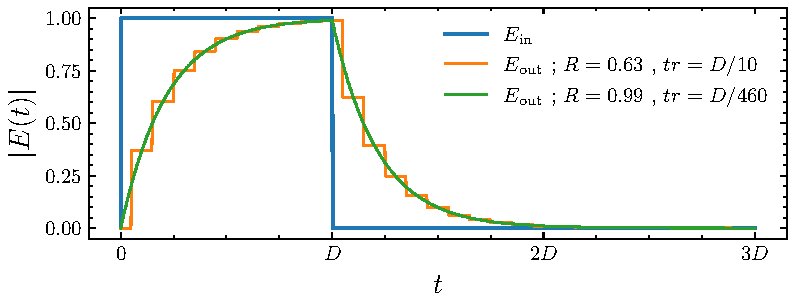
\includegraphics[width=0.7\linewidth]{diagrams/cav_pulse}
	\caption{Plots of (\ref{crds_finite_pulse_onRes}), the output response of an optical cavity to a finite monochromatic pulse which has optical frequency which is tuned to a maximum of the steady state response (\ref{cav_airy}). The magnitude of the electric field incident to the cavity is shown in blue, while two different cavity responses are shown in orange and green. The two responses correspond to a long cavity with low reflectivity and a short cavity with high reflectivity, both keeping the ratio $L/(1-R)$ the same. For the long cavity, the steps are due to the long propagation delay between the mirrors. For cavities of practical length, the green trace is more representative.}
	\label{fig:cavpulse}
\end{figure}

\subsubsection{Off Resonance}

For a monochromatic pulse having optical frequency which does not perfectly match one of the cavity modes, we must use the more general equation (\ref{crds_finite_pulse_general}) for the output field. Using parameters for $t_r$ and $R$ corresponding to a short cavity having high reflectivity mirrors, the plot of equation (\ref{crds_finite_pulse_general}) is shown in Fig. \ref{fig:cavpulsedetuned} for several optical frequencies detuned away from perfect resonance with the cavity.

From these results, we make three key observations
\begin{itemize}
	\item The rate of buildup
	\item The damped oscillations
	\item The ringdown after the pulse has ended
\end{itemize}

\begin{figure}[H]
	\centering
	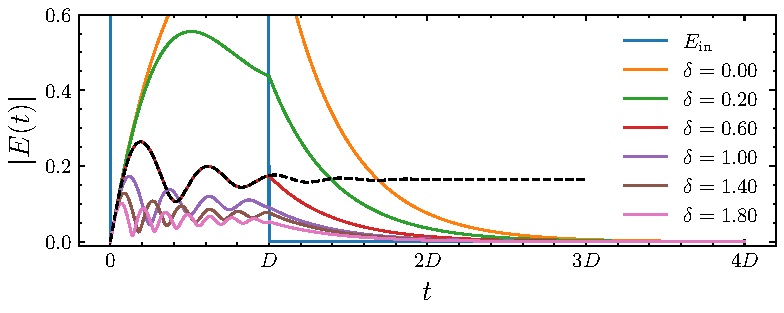
\includegraphics[width=0.7\linewidth]{diagrams/cav_pulse_detuned}
	\caption{Cavity response to a pulsed laser which has wavelength tuned away from the cavity resonance. The electric field amplitude is shown by the blue curve. The detuning from the resonance, $\delta$, gives the frequency of the damped oscillations which occur in the cavity output upon excitation. If the pulse duration $D$ was made long enough, the oscillations would dampen into the constant steady state response given by (\ref{cav_airy}), as shown by the dashed black curve. When the exciting laser is switched off, a clean ringdown transient is observed.}
	\label{fig:cavpulsedetuned}
\end{figure}
It is clear that the maximum buildup rate of the light intensity coming from the cavity corresponds to that which is obtained when the laser and cavity are on resonance (this is the orange trace in Fig. \ref{fig:cavpulsedetuned}). Using the result (\ref{crds_finite_pulse_onRes_approx}) for a short cavity having high reflectivity mirrors, this maximum buildup rate is then
\begin{equation}
	\frac{d\left|E_\mathrm{out}\right|}{dt}\Bigg|_{t=0} = \frac{T}{1-R}\frac{\sqrt{R}}{2\tau_0}
\end{equation}

During the moments when the pulse is switched on, only the first $\theta$ function in (\ref{crds_finite_pulse_general}) is nonzero. We have for the electric field magnitude
\begin{align} \label{cav_pulse_during}
	\left|E_\mathrm{out}\right|^2 &= \frac{T^2}{\left|1-r^2 e^{-i\omega t_r}\right|^2} \left|
	1 - \left(r^2 e^{-i \omega t_r}\right)^{N_1+1}
	\right|^2 \nonumber \\
	&= I_\mathrm{out}(\omega) \;
	\left|
	1 - \left(r^2 e^{-i \omega t_r}\right)^{N_1+1}
	\right|^2
\end{align}
Is is now seen that the output intensity of the cavity approaches the value given by the Airy formula (\ref{cav_airy}) for $I_\mathrm{out}(\omega)$, but with a damped oscillatory factor which determines the transient behavior. In the limit of high reflectivity and short cavity length, the stair-step behavior becomes a continuous one. For this we make the replacement from the discrete $N_1$ to a continuous one $N_1 \rightarrow t/t_r -1/2$.
We then have for the exponential term
\begin{align*}
	q \equiv \left(r^2 e^{-i\omega t_r}\right)^{N_1 +1} &= \left(r^2 e^{-i\omega t_r}\right)^{t/t_r + 1/2} \\
	&= \left(r^2 e^{-i\omega t_r}\right)^{1/2} r^{2t/t_r} e^{-i\omega t}
\end{align*}
We write in terms of the detuning $\delta$ from the cavity resonance frequency $\omega_0$ by introducing $\omega= \omega_0 + \delta$. This gives $r^2 e^{-i\omega_0 t_r} = R$. Using the definition for the reflectivity (\ref{cav_R_defin}) and the exact formula (\ref{tau_vac_exact}) for the ringdown time $\tau_0$ gives $r^{2t/t_r} = e^{-t/2\tau_0} e^{-2i\phi t/t_r}$. Together this gives the result
%	\begin{align*}
	%		q &= \left(r^2 e^{-i\omega t_r}\right)^{1/2} e^{-t/2\tau_0} e^{-2i\phi t/t_r} e^{-i\omega t} \\
	%		&= r e^{-t/2\tau_0} e^{-i\omega t_r/2} e^{-2i\phi t/t_r} e^{-i\omega t} \\
	%		&= \underbrace{\sqrt{R} e^{-t/2\tau_0}}_Q \underbrace{e^{-i\phi}e^{-i\omega t_r/2} e^{-2i\phi t/t_r} e^{-i\omega t}}_{e^{-i\phi'}}
	%	\end{align*}
\begin{align*}
	q &= \left(R e^{-i\delta t_r}\right)^{1/2} e^{-t/2\tau_0} e^{-2i\phi t/t_r} e^{-i\delta t} \cancel{e^{-i \omega_0 t}} \\
	&= \underbrace{\sqrt{R} e^{-t/2\tau_0}}_Q \underbrace{e^{-i\delta t_r/2} e^{-2i\phi t/t_r} e^{-i\delta t}}_{e^{-i\phi'}}
\end{align*}
In the second to last line we have removed the term oscillating at $\omega_0$, the optical frequency of the cavity resonance, since the photodetector will not respond to these oscillations. Above we have defined $Q$ and $\phi'$, the magnitude and phase of the quantity $q$, which allow us to write the term on the right of (\ref{cav_pulse_during}) in the simplified notation
\begin{align*}
	\left|E_\mathrm{out}\right|^2 \propto
	\left|1-q\right|^2 = (1-q^*)(1-q) &= 1 + \left|q\right|^2 - 2\Re \left[q\right] \\
	&= 1 + \left|Q\right|^2 - 2\left|Q\right|\cos\phi'
\end{align*}
We can now evaluate (\ref{cav_pulse_during}) in the limit where the pulse duration is much longer than the cavity round trip time, giving the photodetector response during the pulse as the step response
\begin{equation}\label{cav_pulse_analytic}
	\left|E_\mathrm{out}\right|^2 = I_\mathrm{out}(\omega) \left\{1 + R e^{-t/\tau_0} - 2 \sqrt{R} e^{-t/2\tau_0} \cos\left[\left(\delta + \frac{2\phi}{t_r}\right)t + \frac{\delta t_r}{2}\right]\right\}
\end{equation}
We can now see that the transient behavior is governed by a term decaying with a time constant equivalent to the ringdown time, and an oscillatory term which decays with a time constant which is twice the ringdown time. This behavior is reflected in the plots of Fig. \ref{fig:cavpulsedetuned}, where the square root of the above expression is plotted with the dashed black curve, seen to trace on top of the numerical evaluation of (\ref{crds_finite_pulse_general}).

After the pulse is switched off, there is a contribution from both $\theta$ functions in (\ref{crds_finite_pulse_general}). The electric field squared magnitude is
\begin{align}
	\left|E_\mathrm{out}\right|^2
	%&= \frac{T^2}{\left|1-r^2 e^{-i\omega t_r}\right|^2} \left|
	%\left(r^2 e^{-i \omega t_r}\right)^{N_2+1} - 
	%\left(r^2 e^{-i \omega t_r}\right)^{N_1+1}
	%\right|^2 \nonumber \\
	&=I_\mathrm{out}(\omega) \left|
	\left(r^2 e^{-i \omega t_r}\right)^{N_2+1} - 
	\left(r^2 e^{-i \omega t_r}\right)^{N_1+1}
	\right|^2
\end{align}
Again we get the Airy function for the steady state cavity transmission (\ref{cav_airy}), but modulated with an additional factor. We re-write this factor in a form which makes clear the exponential decay observed in Fig. \ref{fig:cavpulsedetuned} after the driving pulse is turned off. Similar to before, we define the factors
\begin{align*}
	q_1 &\equiv \left(r^2 e^{-i\omega t_r}\right)^{N_1 +1} = \underbrace{\sqrt{R} e^{-t/2\tau_0}}_{Q_1} \underbrace{e^{-i\phi}e^{-i\omega t_r/2} e^{-2i\phi t/t_r} e^{-i\omega t}}_{e^{-i\phi_1'}} \\
	q_2 &\equiv \left(r^2 e^{-i\omega t_r}\right)^{N_2 +1} = \underbrace{\sqrt{R} e^{-(t-D)/2\tau_0}}_{Q_2} \underbrace{e^{-i\phi}e^{-i\omega t_r/2} e^{-2i\phi (t-D)/t_r} e^{-i\omega (t-D)}}_{e^{-i\phi_2'}}
\end{align*}
We use this notational simplification to evaluate the magnitude squared difference appearing in the above expression for $\left|E_\mathrm{out}\right|^2$
\begin{align*}
	\left|E_\mathrm{out}\right|^2 \propto
	\left|q_2 - q_1\right|^2 &= (q_2^* - q_1^*)(q_2 - q_1) = \left|q_2\right|^2 + \left|q_1\right|^2 - 2 \Re\left[q_2^* q_1\right] \\
	&= Q_2^2 + Q_1^2 - 2 Q_1Q_2 \cos\left[\phi_1 - \phi_2\right] \\
	%&= Re^{-t/\tau_0}(1 + e^{D/\tau_0})
	&= R e^{-(t-D)/\tau_0} + R e^{-t/\tau_0} - 2 R e^{-t/\tau_0}e^{D/2\tau_0}\cos\left[2\phi D/t_r +\omega D\right] \\
	%&= R\left\{
	%e^{D/\tau_0} + 1 - 2 e^{D/2\tau_0}\cos\left[2\phi D/t_r +\omega D\right]
	%\right\} e^{-t/\tau_0} \\
	&= R \left\{1 +
	e^{-D/\tau_0} - 2 e^{-D/2\tau_0} \cos\left[2\phi D/t_r +\omega D\right]
	\right\}e^{-(t-D)/\tau_0}
\end{align*}

We see from the above result that after the laser is shut off at time $t=D$, we get a photodetector signal proportional to
\begin{equation}
	\left|E_\mathrm{out}\right|^2 = A e^{-(t-D)/\tau_0}
\end{equation}
This important result highlights that, independent of the laser detuning used to excite the cavity resonance, a clean exponential decay is observed when the input field is completely extinguished. It was seen from expression \ref{cav_pulse_analytic} that oscillating terms appear in the cavity output when the light source is still switched on, complicating the determination of the cavity ringdown time.

This is precisely the motivation for the use of an external modulator for the rapid shutoff of the laser \cite{cw_crds_ROMANINI} when resonance between the laser and cavity is achieved. In this work we employ the use of an acousto-optic modulator (AOM), which can easily achieve sub-100ns shutoff times in the first-order deflected output, as well as extremely large extinction ratios.

\subsection{Sweep of the Laser Across the Cavity Resonance} \label{sec:cav_laser_sweep}
For a high finesse cavity, the overlap of any one of the narrow resonances with the narrow laser line has low probability for occurring at random. Mechanical vibrations result in small jitters of the cavity length which cause a subsequent variation of the FSR. The optical frequency $\nu$ of any one resonance is determined from (\ref{cav_resonance_condition}) as $\nu \approx m\mathrm{FSR}$, where the mode number $m\approx2L/\lambda$ is generally large. The jitter of any one mode position is amplified by a factor which grows with the cavity length. Combined with jitter in the laser wavelength, resonance is difficult to maintain for any extended period of time without active locking. Such an active locking scheme is explored in Sec. \ref{sec:pdh_ringdown}.

A simple method for reliably obtaining short periods of laser-cavity resonance is two sweep either the laser frequency by at least one FSR, or by scanning the cavity length one-half of the laser wavelength. This exploits the repeating mode structure of the cavity by always scanning a size greater than this period. In this section, we make numerical and analytical predictions of a cavity which has a swept laser as input.

We consider here the case of a laser with controllable wavelength which can continuously sweep the across the resonance of an optical cavity. Such a configuration can be used to track the wavelength of the scanning laser, and this was the case for our work on the precision measurement of the xenon hyperfine structure \cite{ours_xe_paper}. As the scan rate is increased, the effect of a finite ringdown time becomes apparent in the signal and can be used to conduct cavity ringdown spectroscopy \cite{crds_rapidSweep_Debecker_05}.

We consider the case of an input field which has a linearly varying instantaneous frequency
\begin{equation}
	E_\mathrm{in}(t) = e^{-i\left[\omega_0 + \frac{1}{2}a t\right]t}
\end{equation}
The derivative of the complex phase gives the instantaneous frequency as $\omega(t) = \omega_0 + a t$. The constant $a$ is the scan rate of the laser in $\mathrm{rad}/\mathrm{s}/\mathrm{s}$.

Plots of the cavity output response (\ref{cav_output_field}) for this particular input field are shown in Fig. \ref{fig:cavsweeps}. For a slow sweep, the output exactly mimics equation (\ref{cav_airy}) for the steady state response. As the sweep rate is increased, the effects of the finite response time of the cavity become apparent as the response becomes shifted, distorted, and diminished. This effect is exaggerated for a high finesse cavity, which is shown in the far-right viewgraph of Fig. \ref{fig:cavsweeps}. Even though the laser spends very little time having its instantaneous frequency resonant with the cavity, the cavity has appreciable output on a time scale comparable to the ringdown time. 

\begin{figure}[H]
	\centering
	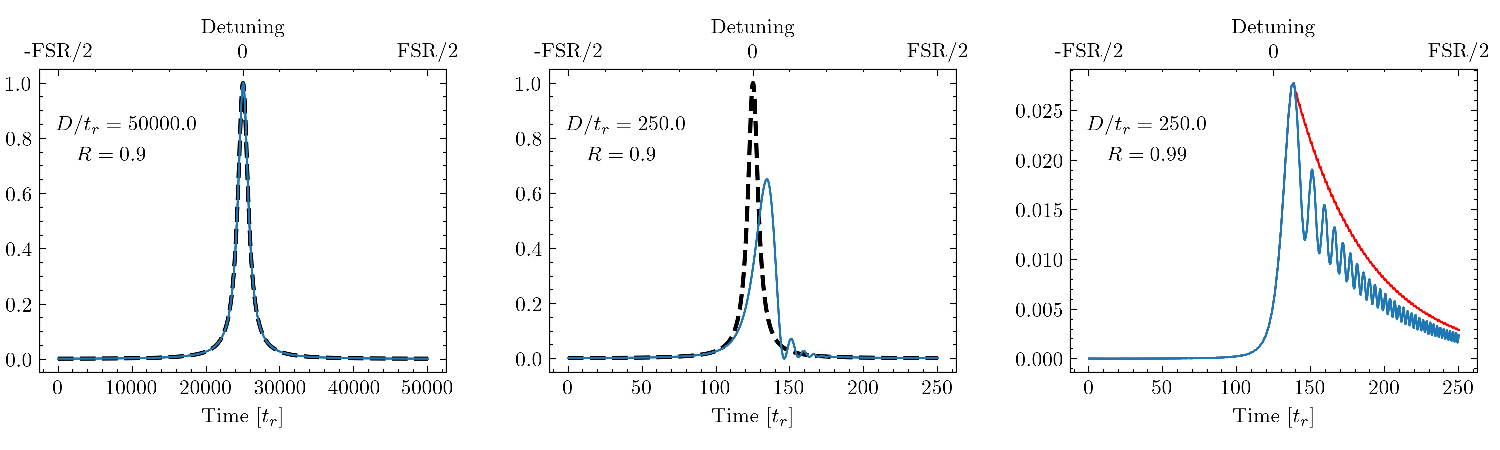
\includegraphics[width=1.0\linewidth]{diagrams/cav_sweeps}
	\caption{Shown is the output of a stationary cavity having its input laser swept in wavelength. Two scanning speeds (proportional to $D/t_r$) are shown; the left graph shows a very slow laser scan accross the resonance, and the middle and right graphs have an increased scanning speed. The cavity finesse is increased from the middle graph to the right graph. For a slow scan across the resonance of low-finesse cavity, the steady state response given by (\ref{cav_airy}), shown with the dashed black plot, is approximately traced out. As the scan speed is increased, the distortion of the transient signal away from the steady state response becomes apparent. Increasing the cavity finesse for a fixed scan speed exaggerates this effect even further, as seen on the rightmost plot. The red curve shown on the right is the effect of turning off the input laser excitation at the output peak, giving a clean ringdown transient. It can be seen that for the rapidly swept case, the rough profile follows this exponential decay.}
	\label{fig:cavsweeps}
\end{figure}

In the right-most viewgraph of the above figure, we consider the rapid sweep of a laser wavelength through a the resonance of a high finesse cavity. The resonance for this cavity is $\sim$10x narrower than for the other cavities shown, and is apparent that the peak response occurs well after the laser has detuned off resonance. Shown also in this right-most viewgraph in red is the response of the cavity if the laser had been instantaneously shut off at the moment of this peak response. It is therefore clear that destructive interference with the input light is the cause of departure from a clean exponential decay. Again, we see the efficacy of using an external modulator to shut off the laser in a time which is small compared to the round trip time of the cavity $t_r$.

\subsubsection{Integral of the Swept Output}
Direct determination of the ringdown time $\tau_0$ of a cavity requires that the transmitted light be detected on sub-microsecond time scale. For a detector which operates much more slowly than this, the output will be proportional to the integral of a single resonance event. That is, we seek a relation of $\int \left|E_\mathrm{out}(t)\right|^2 dt$ for the swept laser input field, integrated over a resonance event.

The time-domain response of the cavity is given by (\ref{cav_output_field}), which gives for the above input field
\begin{align}
	E_\mathrm{out}(t) &= T\sum_{m=0}^{\infty}r^{2m}\exp\left\{-i\omega_0\left(t - \frac{t_r}{2} - mt_r\right)\right\} \exp\left\{ -i\frac{a}{2}\left(t - \frac{t_r}{2} - mt_r\right)^2\right\} \\
	&= e^{-i\omega_0\left(t - t_r/2\right)}e^{-i\frac{a}{2}\left(t - t_r/2\right)^2} T \sum_{m=0}^{\infty}R^{m}e^{i\omega_0 mt_r - i\frac{a}{2}\left(mt_r\right)^2 + iamt_r (t-t_r/2) - 2im\phi} 
\end{align}
We have a sum of the form $S\equiv \sum_{m=0}^{\infty}R^m e^{-i\alpha\left(m^2 - \beta m\right)}$, with the following definitions
\begin{eqnarray}
	\alpha \equiv \frac{at_r^2}{2} &\qquad& \beta \equiv \frac{2\omega_0}{at_r}+ \frac{2}{t_r}\left(t - \frac{t_r}{2}\right) - \frac{4\phi}{at_r^2}
\end{eqnarray}
We can complete the square for the term in the exponential argument \newline $-i\alpha\left[m^2 - \beta m\right] =  -i \alpha \left[\left(m-\frac{\beta}{2}\right)^2 - \frac{\beta^2}{4}\right]$ which allows us to write the sum as
\begin{align*}
	S &= e^{i\alpha \beta^2/4} \sum_{m=0}^{\infty}R^m e^{-i\alpha (m-\beta/2)^2}
\end{align*}

The photodetector response is proportional to the magnitude squared of the cavity output field. The many complex exponential factors appearing in front of the field expression are canceled under this operation, leaving
\begin{align*}
	\left|E_\mathrm{out}(t)\right|^2 &= T^2\left(\sum_{m=0}^{\infty} R^m e^{-i\alpha (m-\beta/2)^2}\right)\left(\sum_{n=0}^{\infty} R^n e^{i\alpha (n-\beta/2)^2}\right) \\
	&= T^2\sum_{m=0}^{\infty}R^{2m} + 2T^2 \sum_{m=0}^{\infty}\sum_{n=m+1}^{\infty}\Re \left\{R^{m+n} e^{i\alpha\left[(m-\beta/2)^2 - (n-\beta/2)^2\right]}\right\} \\
	%&= T^2\sum_{m=0}^{\infty}R^{2m} + 2T^2 \sum_{m=0}^{\infty}\sum_{n=m+1}^{\infty}R^{2m}\cos \left\{\alpha\left[(m-\beta/2)^2 - (n-\beta/2)^2\right]\right\} \\
	&= T^2\sum_{m=0}^{\infty}R^{2m} + 2T^2 \sum_{m=0}^{\infty}\sum_{n=m+1}^{\infty}R^{m+n}\cos \left\{\alpha\left[m^2 - n^2 + (n-m)\beta\right]\right\} \\
	&= \frac{T^2}{1-R^2} + 2T^2 \sum_{m=0}^{\infty}\sum_{n=m+1}^{\infty}R^{m+n}\cos \Bigg\{\frac{at_r^2}{2}\left[m^2 - n^2 + (n-m)\left(\frac{2t}{t_r} - 1\right)\right] \nonumber\\
	&\qquad\qquad\qquad\qquad\qquad\qquad\qquad\qquad\qquad
	+ (n-m)\left(\omega_0 t_r - 2\phi\right)\Bigg\}
\end{align*}
The argument to the cosine function in the above nested sum is of the simple form
\begin{equation*}
	\cos\left[(n-m) a t t_r + \Phi(n,m,t_r,\omega_0)\right]
\end{equation*}
If we set the scanning rate such that one free spectral range is scanned in a time $D$, we have $a=2\pi/t_rD$. We can guarantee that each of the cosine terms in the above nested sum integrates to zero by choosing the integration time from $0$ to $D$. This trivially gives the integral of the photodetector signal of the cavity output for the swept laser as
\begin{equation}
	\int_{0}^{D}\left|E_\mathrm{out}(t)\right|^2 dt = \frac{DT^2}{1-R^2} \simeq \frac{T^2 D}{t_r}\tau_0
\end{equation}

We now come to the conclusion that the integral of the cavity output light is proportional to the ringdown time of the cavity $\tau_0$. For a slow detector, this observation allows us to determine the ratio of two ringdown times $\tau/\tau_0$. In general, direct determination of the ringdown time from such an expression is tricky since we must resolve the proportionality constant, which includes the detector gain. It is much easier to measure two such events, keeping the proportionality constant the same, and take the ratio. This is the principle by which absorption is computed in some instances of Vernier spectroscopy, especially those where a slow focal plane array detector is used.

The proportionality to $\tau_0$ is most easily seen from the simple case of a clean exponential decay emerging from the cavity
\begin{equation*}
	\int_{0}^{\infty} A e^{-t/\tau_0} = A\tau_0
\end{equation*}

\subsection{Sweep of the Cavity Resonance Across the Laser}
Here we consider the case of a linear cavity having its round trip length changed as a function of time. This corresponds to the realistic case of a cavity having a piezo electric actuator attached to one of the mirrors, allowing a slight modulation of the cavity length $L\rightarrow L(t)$. For now we consider the case of a cavity mirror moving at a constant velocity, giving the time dependent length
\begin{equation}
	L(t) = L_0 + vt
\end{equation}

We cannot use equation (\ref{cav_output_field}) as before. Return to the construction of Fig. \ref{fig:cavitytransmission}, the cavity output field in response to monochromatic input $E_\mathrm{in}(t) = E_0 e^{-i\omega t}$ is then \cite{crds_ultraslow_velocities, Gohle_Dissertation_2006}
\begin{equation}
	E(t) = E_0 t^2 \sum_{n=0}^{\infty}r^{2m}\exp\left\{i\frac{\omega}{c}\left[L + 2\sum_{m=1}^{n}L(t_m)\right] - i\omega t\right\}
\end{equation}

\begin{equation}
	t_m = t - \frac{(2m-1)L_0}{c}
\end{equation}

%In order to compute the response of this length-modulated optical cavity to an arbitrary input field, we must upgrade expression (\ref{cav_output_field}) to include the changing delay of the cavity. We remind the reader that expression (\ref{cav_output_field}) can be directly obtained by the construction of Fig. \ref{fig:cavitytransmission}, and we can perform the upgrade of this expression using the same construction. Denoting the complex transmission coefficient as $\tilde{t}$ to avoid confusion with time, the beamlets in Fig. \ref{fig:cavitytransmission}(b) have the time-dependent delay

For $v/c<<1$, the sum in the exponent can be evaluated
\begin{align}
	\sum_{m=1}^{n}L(t_m) &= \sum_{m=1}^{n}\left(L_0 + v t_m\right) \\
	&= n\left[\left(1-n\frac{v}{c}\right)L_0 + vt\right] \\
	&= nc\left[(1-n\beta)\frac{t_r}{2} + \beta t\right]
\end{align}

This gives the cavity output as
\begin{equation}
	E(t) = E_0 e^{i(\omega L_0/c - \omega t)}\sum_{n=0}^{\infty}r^{2n}\exp\left\{i2n\omega\left[(1-n\beta)\frac{t_r}{2} + \beta t\right]\right\}
\end{equation}

We can see that when illuminated with light of a single frequency $\omega$, the cavity output features many additional frequencies. This non-linearity of the output means that we cannot represent the swept cavity output by a simple transfer function. This can be intuitively understood by the doppler shift of the light which is reflected from the moving mirror. Upon each reflection, the light experiences a doppler shift of its frequency. After many reflections in the cavity, the many doppler shifts of the beam give a mixture of frequencies which were not originally present in the beam.

\subsection{Time Domain Signal of CRDS} \label{sec:cav_crds}

In this section we attempt to model a realistic transient of a cavity resonance swept across a laser line, with the laser light being shut off during the excitation. Such a configuration is common for CRDS, where a swept cavity is used to guarantee a resonance condition with laser light of arbitrary wavelength, and an external modulator to rapidly extinguish the incident light in the middle of the excitation.

Plotted in Fig. \ref{fig:crds_aomsimulation} is the ratio $\left|E_\mathrm{out}\right|/\left|E_\mathrm{in}\right|$ for two different cavities, on the left having $R=0.99$ and on the right $R=0.998$, and both cavities are swept at identical rates. Overlayed on both plots is the result of shutting off the exciting laser at different times.

\begin{figure}[H]
	\centering
	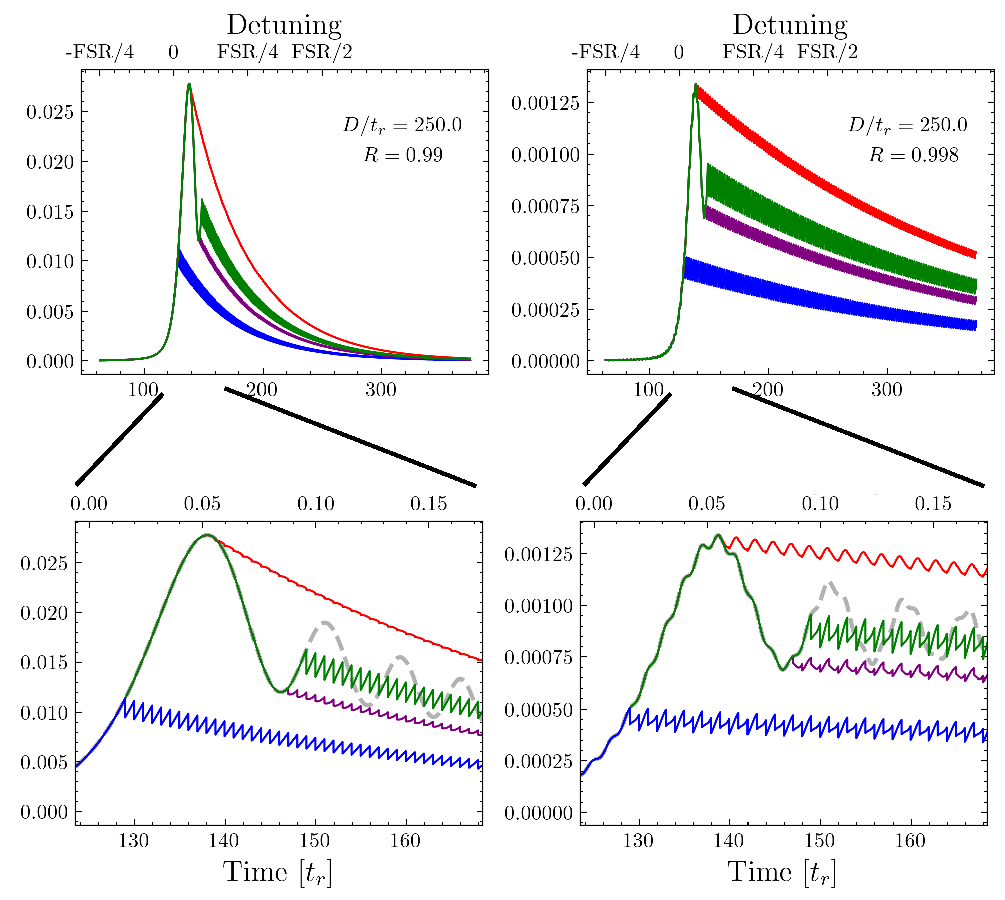
\includegraphics[width=0.7\linewidth]{diagrams/crds_AOMsimulation}
	\caption{Simulated output of a cavity with scanning length having a laser with stationary wavelength mode-matched to the input. The black dashed curve shows the transient response of the cavity for a laser that is always on. The colored curves correspond to different places in the transient where the exciting laser is switched off. It can be seen that the effect of switching off the laser near the onset of resonance is to give a curve which decays exponentially and is superimposed with harmonics of the cavity FSR. For a high-finesse cavity, these harmonics are easily filtered from the cavity transient by electronic filters. It can also be seen that the effect of switching off the laser is to eliminate lower frequency beating behavior which is much more difficult to eliminate. It is therefore almost always preferable to use an external modulator to eliminate these effects from CW ringdown measurements.}
	\label{fig:crds_aomsimulation}
\end{figure}

It can be seen that after the exciting laser is shut off, the signal follows an exponential decay which has a $1/e$ constant of $\tau$ the cavity ringdown time. This exponential decay is accompanied by high frequency beating having frequencies which are harmonics of the cavity FSR, a fact which is established by the fact that the beating is periodic with period $t_r = 1/\mathrm{FSR}$. It can be seen from Fig. \ref{fig:crds_aomsimulation} that the amplitude of the beating signal is dependent on the part of the exitation curve where the laser is shut off, having minimum amplitude when the shutoff time corresponds to a critical point of the output light.

From our previous discussion, we may surmise that the post-shutoff CRDS signal has the form
\begin{equation}
	I(t) = A e^{-t/\tau} + B(t) e^{-t/2\tau}
\end{equation}

The beating terms are described by a function $B(t)$ which is periodic with period $t_r$, the round-trip time of the cavity. If the ringdown time $\tau$ of the cavity is much longer than the cavity round-trip time, these beating signals may be effectively filtered out by a lowpass filter. Performing this filtering of the beating signals removes the requirement that the digital acquisition system operate at a sampling rate which is multiple times the FSR of the cavity, otherwise these high frequency beat signals will be aliased into ripples. By filtering the high frequency beat notes, the acquisition system can then be optimized for the measurement of a clean exponential signal

\begin{equation}
	I_\mathrm{filtered}(t) = A e^{-t/\tau} + O
\end{equation}

In the above expression $O$ represents a residual offset from the filtering process. In practice, this term can encompass other experimental factors such as offsets from photodetector amplifiers and the calibration of the voltage offset of the acquisition system. The above expression serves as a sufficient fitting model for experimental measurements of decaying post-shutoff light emerging from an excited optical cavity, and it is this model that we will use for fitting ringdown curves in this dissertation.

\section{Experimental Realization of Cavity Properties}
In this section we demonstrate experimentally some of the theoretical results of the previous section. These will be focused on methods of resolving the cavity mode structure, which aids in the alignment of the input beam, and the measurement of the cavity ringdown time, which is important for sensitive spectroscopic measurements.

\subsection{Higher Order Mode Structure} \label{sec:cav_alignment}
When aligning a laser beam to an optical cavity, the coupling is very sensitive to the propagation direction of the beam even when the transverse profile is perfectly mode matched to the cavity (Sec. \ref{sec:mode-matching}). An exception is made for the confocal cavity, which has the greatest acceptance of the input beam \cite{book_lasers_siegman}.

A slightly misaligned beam will cause excitation of higher order modes spatial modes in the cavity, and these can be detected in the transmission of the cavity. We can optimize the laser-cavity coupling by minimizing the excitation of these higher order cavity modes and maximizing the excitation of the fundamental mode. The relative excitation of the higher order modes may be realized using the fact that the higher order modes generally have a different resonance frequency than the fundamental modes. For a Hermite-Gauss mode having indices $m$ and $n$, there is an additional Guoy phase shift which shifts the location of the resonance. For a cavity having round trip length $\ell$, the round trip phase shift must be a multiple of $2\pi$, so the modes higher order modes must satisfy \cite{book_lasers_siegman}
\begin{equation}
	\frac{\omega \ell}{2c} - \left(n + m + 1\right)\cos^{-1}\pm \sqrt{g_1 g_2} = q \pi
\end{equation}
where $q$ is an integer. The $g_{1,2}$ parameters were defined in Sec. \ref{sec:cav_ABCD} as the dimensionless parameters defining the cavity geometry. In terms of these parameters, the resonance frequencies are then given by
\begin{equation} \label{cav_higherOrder_mode_freqs}
	\nu_{qmn} = \left[q + (n + m + 1) \frac{\cos^{-1}\pm\sqrt{g_1 g_2}}{\pi}\right] \frac{c}{\ell}
\end{equation}
The factor $\cos^{-1}\pm\sqrt{g_1 g_2}/\pi$ is bounded by $\pm 1$, so the higher order modes generally appear between the axial resonances, here enumerated by $q$. For the linear cavity shown in Fig. \ref{fig:cavitymodematch} we have $g_1 = 1$ (corresponding to the flat mirror). The cavity dimensions $L=1.72m$ and $R=2m$, give $g_2 \approx 0.14$. The higher order modes are located at a fraction $\cos^{-1}\pm\sqrt{g_1 g_2}/\pi \approx 0.38$ of the free spectral range.

Using a laser of fixed wavelength, we can scan these resonances by slightly modulating the cavity length using a piezoelectric actuator attached to one of the cavity mirrors. As the length of the cavity is scanned different modes come into resonance with the laser. If the scan amplitude is large enough, a repeating pattern of resonances will be observed corresponding to the free spectral range of the cavity. In Fig. \ref{fig:cavalignmentmodes}, we show such a scan of a cavity in a misaligned condition, where a higher order mode is seen at roughly one-third of the scan of the free spectral range, in agreement with our calculation for this cavity. The same cavity is shown after adjusting the cavity alignment to suppress the excitation of this higher order mode.

\begin{figure}[H]
	\centering
	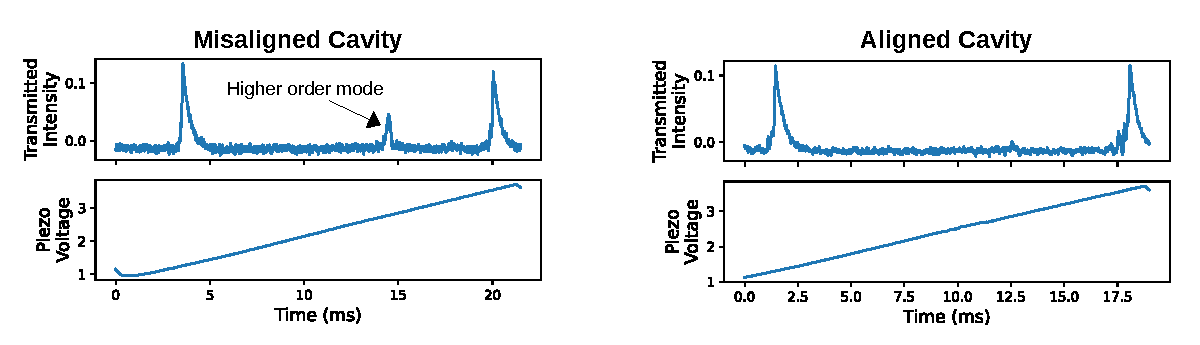
\includegraphics[width=1.0\linewidth]{diagrams/cav_alignmentModes}
	\caption{The final alignment of an optical cavity can be performed by observing the transmitted mode structure when the cavity length is scanned by changing the voltage applied to a piezoelectric actuator. In both graphs, the spacing between the large transmitted peaks represents the free spectral range of the cavity. Appearing on the left graph between these larger peaks is a smaller peak which is evidence of a transmitted higher mode. By adjusting the laser-cavity alignment, the graph on the right is obtained where the higher-order mode excitation is nearly extinguished. The relative spacing of the higher order modes compared to the FSR are given by (\ref{cav_higherOrder_mode_freqs}).}
	\label{fig:cavalignmentmodes}
\end{figure}

Critical to this alignment is the ability to recognize the repeating pattern of modes corresponding to a complete scan of one free spectral range. This task can be slightly complicated when the location of the higher order modes form evenly spaced locations. In the linear cavity example, the higher order modes form at appoximately 1/3 the free spectral range spacing. When the cavity is severly misaligned, we see the presence of the next higher order mode at 2/3 of the FSR spacing which gives the impression that the repeating pattern is three times smaller than it actually is.

\subsection{On-Resonant Behavior of the Cavity Output} \label{sec:pdh_ringdown}
In sec. \ref{sec:cav_td_response}, we showed that the cavity has a simple filtering behavior for intensity fluctuations of on-resonant monochromatic input light. The characteristic time of this filtering gives a measure of the cavity ringdown time. In this section we show how a direct measurement of this effect could be conducted in practice, leading to a method which can directly measure the ringdown time of the cavity in the most rapid possible manner.

For a high finesse cavity, it is difficult to ensure overlap of the narrow cavity mode with the laser wavelength. Mechanical vibrations in the optical setup cause jitter in the location of any one cavity resonance, and unless active stabilization methods are used, the laser also experiences jitter in the output wavelength. One such active stabilization technique is the Pound-Drever-Hall technique \cite{PDH_locking} for locking a laser's wavelength to a cavity resonance. This technique can also be modified to instead stabilize the cavity length, where the location of a single cavity resonance is locked to the laser wavelength.

Shown in Fig. \ref{fig:cavpdhlock} is a ring cavity which has been modematched to an input laser beam. The beam profile and modematching condition were shown for this particular cavity in Fig. \ref{fig:cavitymodematch}. The input beam first passes through an electro-optic modulator (EOM) which puts phase modulation sidebands on the optical spectrum of the laser. In the presence of the cavity resonance the sidebands are unbalanced, creating a beat note at the EOM driving frequency which is seen at the reflection photodiode. This signal (shown in orange) is demodulated using a double balance mixer and low pass filter which gives a signal which is approximately the derivative of the resonance signal (shown in yellow). This is used as an error signal since it has a linear zero crossing at the point of resonance. The servo loop uses this error signal to provide correction to the cavity length via the piezo electric actuator which is shown in the diagram as PZT.

We note that this is slightly different than the original conception of the Pound-Drever-Hall technique \cite{PDH_locking}, where the feedback is applied to the cavity instead of the laser. In certain cases this is desirable, since it may be possible that the laser line is more stable than the cavity resonance.

In Fig. \ref{fig:cavpdhlock} we have also shown an AOM, which allows the intensity of the laser beam to be rapidly modulated by changing the amplitude of the driving RF signal. For this laser, the optical power could not be adjusted independently of the wavelength, so the AOM is used to provide a square wave modulation to the optical power input to the cavity. When the cavity is locked to the laser using the PDH technique, we investigate the cavity response to a square wave modulated input.


\begin{figure}[H]
	\centering
	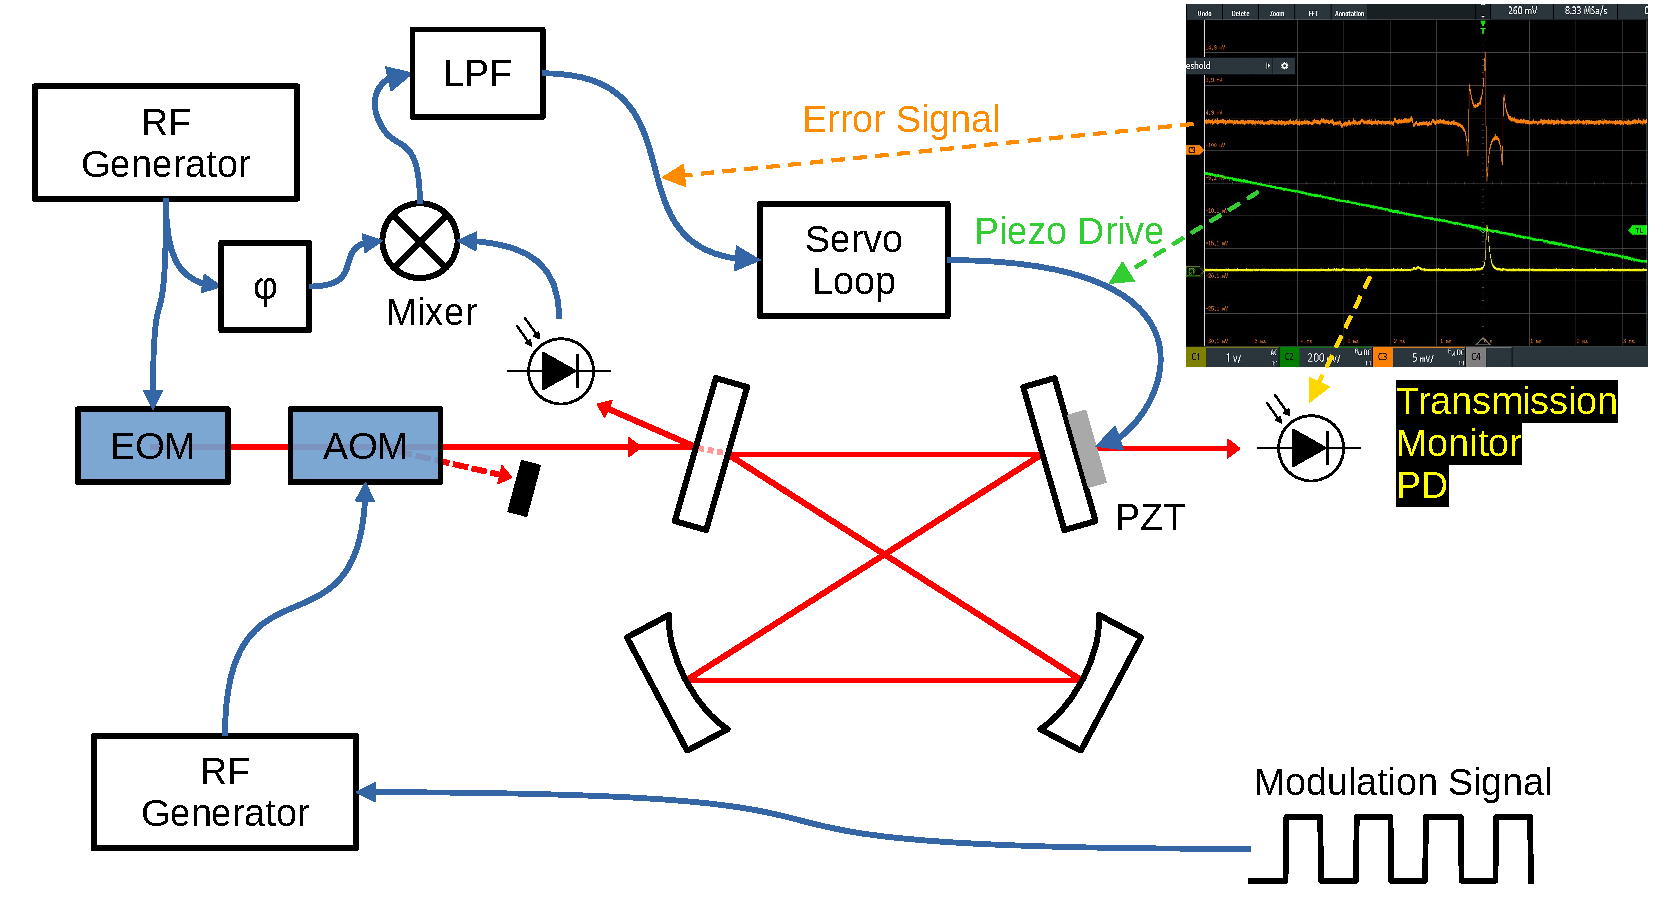
\includegraphics[width=0.7\linewidth]{diagrams/cav_pdhLock}
	\caption{A setup for the stabilization of an optical cavity length to ensure that the laser and cavity are always on resonance. Stabilization is performed using the Pound-Drever-Hall technique, and feedback is performed on a piezoelectric actuator (PZT) attached to one of the cavity mirrors. By modulating the power of the input laser beam, the ringdown time is extracted by the filtering action of the cavity on the output light. This scheme represents the fastest possible ringdown time measurement method, being limited only by the duration of the ringdown transient itself.}
	\label{fig:cavpdhlock}
\end{figure}

It can be seen from the results in Fig. \ref{fig:cavpdhlockoutput} that the cavity response to a square-wave modulated input has the same behavior that was found from the theoretical analysis in the previous section. In fact, the response is well modeled by the equation (\ref{crds_finite_pulse_onRes_approx}), which means that the ringdown time can be extracted by fitting the response.

\begin{figure}[H]
	\centering
	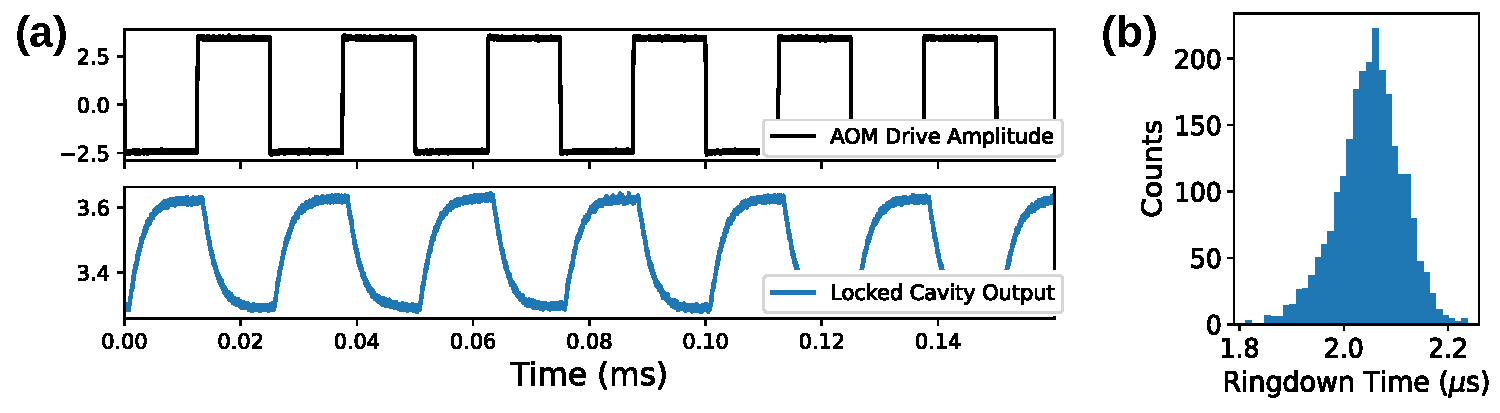
\includegraphics[width=0.8\linewidth]{diagrams/cav_pdhLock_output}
	\caption{Response of the locked cavity to the intensity modulated input light. The black trace shown in \textbf{(a)} is the trigger signal which enables and disables the RF drive for the AOM. This causes the light input light, having its wavelength locked to the cavity resonance, to be intensity modulated due to some of the light being deflected into the first order output of the AOM. The lower blue trace is the response of the cavity to the on-resonant intensity modulated light. The resemblance to the theoretical response shown in Fig. \ref{fig:cavpulse} is clear. Shown in \textbf{(b)} is the result of fitting many of the transitions to extract the ringdown time. The acquisition rate of 4kHz shown here is essentially the fastest possible for this cavity, as shortening the observation duration negatively impacts the retrieved fits.}
	\label{fig:cavpdhlockoutput}
\end{figure}

The proof-of-concept setup presented here illustrates the fastest possible acquisition scheme for ringdown transients. Since the laser is always on resonance with the cavity, no time is spent waiting for the laser or cavity to scan onto resonance with one another. Even in this tightly locked scheme, we are ultimately limited by the length of the ringdown transient itself. If for accurate fitting, we require $\sim 5\tau$, then the maximum possible acquisition rate is $1/5\tau$.

%	\subsection{Off-Resonant Behavior of the Cavity Output}
%	\begin{itemize}
	%		\item \textbf{\hl{Show the CRDS-style "sweep onto resonance" configuration in its simplest form.}}
	%		\item \textbf{\hl{Emphasis on the hardware simplification this brings.}}
	%	\end{itemize}

%	\begin{appendices}
%		\titleformat{\chapter}{\centering\normalsize}{APPENDIX \thechapter}{0em}{\vskip .5\baselineskip\centering}
%		\renewcommand{\appendixname}{APPENDIX}
%		
%		
%		%\input{appendices/A2_Second}
%		
%	\end{appendices}

\end{document}